\documentclass[twoside]{book}

% Packages required by doxygen
\usepackage{calc}
\usepackage{doxygen}
\usepackage{graphicx}
\usepackage[utf8]{inputenc}
\usepackage{makeidx}
\usepackage{multicol}
\usepackage{multirow}
\usepackage{textcomp}
\usepackage[table]{xcolor}

% Font selection
\usepackage[T1]{fontenc}
\usepackage{mathptmx}
\usepackage[scaled=.90]{helvet}
\usepackage{courier}
\usepackage{amssymb}
\usepackage{sectsty}
\renewcommand{\familydefault}{\sfdefault}
\allsectionsfont{%
  \fontseries{bc}\selectfont%
  \color{darkgray}%
}
\renewcommand{\DoxyLabelFont}{%
  \fontseries{bc}\selectfont%
  \color{darkgray}%
}

% Page & text layout
\usepackage{geometry}
\geometry{%
  a4paper,%
  top=2.5cm,%
  bottom=2.5cm,%
  left=2.5cm,%
  right=2.5cm%
}
\tolerance=750
\hfuzz=15pt
\hbadness=750
\setlength{\emergencystretch}{15pt}
\setlength{\parindent}{0cm}
\setlength{\parskip}{0.2cm}
\makeatletter
\renewcommand{\paragraph}{%
  \@startsection{paragraph}{4}{0ex}{-1.0ex}{1.0ex}{%
    \normalfont\normalsize\bfseries\SS@parafont%
  }%
}
\renewcommand{\subparagraph}{%
  \@startsection{subparagraph}{5}{0ex}{-1.0ex}{1.0ex}{%
    \normalfont\normalsize\bfseries\SS@subparafont%
  }%
}
\makeatother

% Headers & footers
\usepackage{fancyhdr}
\pagestyle{fancyplain}
\fancyhead[LE]{\fancyplain{}{\bfseries\thepage}}
\fancyhead[CE]{\fancyplain{}{}}
\fancyhead[RE]{\fancyplain{}{\bfseries\leftmark}}
\fancyhead[LO]{\fancyplain{}{\bfseries\rightmark}}
\fancyhead[CO]{\fancyplain{}{}}
\fancyhead[RO]{\fancyplain{}{\bfseries\thepage}}
\fancyfoot[LE]{\fancyplain{}{}}
\fancyfoot[CE]{\fancyplain{}{}}
\fancyfoot[RE]{\fancyplain{}{\bfseries\scriptsize Generated on Mon Nov 30 2020 17\-:06\-:11 for Nysse Meni -\/ kaupunkiseikkailu Tampereella by Doxygen }}
\fancyfoot[LO]{\fancyplain{}{\bfseries\scriptsize Generated on Mon Nov 30 2020 17\-:06\-:11 for Nysse Meni -\/ kaupunkiseikkailu Tampereella by Doxygen }}
\fancyfoot[CO]{\fancyplain{}{}}
\fancyfoot[RO]{\fancyplain{}{}}
\renewcommand{\footrulewidth}{0.4pt}
\renewcommand{\chaptermark}[1]{%
  \markboth{#1}{}%
}
\renewcommand{\sectionmark}[1]{%
  \markright{\thesection\ #1}%
}

% Indices & bibliography
\usepackage{natbib}
\usepackage[titles]{tocloft}
\setcounter{tocdepth}{3}
\setcounter{secnumdepth}{5}
\makeindex

% Hyperlinks (required, but should be loaded last)
\usepackage{ifpdf}
\ifpdf
  \usepackage[pdftex,pagebackref=true]{hyperref}
\else
  \usepackage[ps2pdf,pagebackref=true]{hyperref}
\fi
\hypersetup{%
  colorlinks=true,%
  linkcolor=blue,%
  citecolor=blue,%
  unicode%
}

% Custom commands
\newcommand{\clearemptydoublepage}{%
  \newpage{\pagestyle{empty}\cleardoublepage}%
}


%===== C O N T E N T S =====

\begin{document}

% Titlepage & ToC
\hypersetup{pageanchor=false}
\pagenumbering{roman}
\begin{titlepage}
\vspace*{7cm}
\begin{center}%
{\Large Nysse Meni -\/ kaupunkiseikkailu Tampereella }\\
\vspace*{1cm}
{\large Generated by Doxygen 1.8.5}\\
\vspace*{0.5cm}
{\small Mon Nov 30 2020 17:06:11}\\
\end{center}
\end{titlepage}
\clearemptydoublepage
\tableofcontents
\clearemptydoublepage
\pagenumbering{arabic}
\hypersetup{pageanchor=true}

%--- Begin generated contents ---
\chapter{Namespace Index}
\section{Namespace List}
Here is a list of all namespaces with brief descriptions\-:\begin{DoxyCompactList}
\item\contentsline{section}{\hyperlink{namespace_student_side}{Student\-Side} \\*Namespace Studen\-Side, Students own imlplementations to project }{\pageref{namespace_student_side}}{}
\item\contentsline{section}{\hyperlink{namespace_ui}{Ui} \\*Namespace \hyperlink{namespace_ui}{Ui} for dialog window class }{\pageref{namespace_ui}}{}
\end{DoxyCompactList}

\chapter{Hierarchical Index}
\section{Class Hierarchy}
This inheritance list is sorted roughly, but not completely, alphabetically\-:\begin{DoxyCompactList}
\item I\-Actor\begin{DoxyCompactList}
\item \contentsline{section}{Student\-Side\-:\-:Actor}{\pageref{class_student_side_1_1_actor}}{}
\end{DoxyCompactList}
\item I\-City\begin{DoxyCompactList}
\item \contentsline{section}{Student\-Side\-:\-:City}{\pageref{class_student_side_1_1_city}}{}
\end{DoxyCompactList}
\item I\-Statistics\begin{DoxyCompactList}
\item \contentsline{section}{Student\-Side\-:\-:Statistics}{\pageref{class_student_side_1_1_statistics}}{}
\end{DoxyCompactList}
\item I\-Vehicle\begin{DoxyCompactList}
\item \contentsline{section}{Student\-Side\-:\-:Vehicle}{\pageref{class_student_side_1_1_vehicle}}{}
\end{DoxyCompactList}
\item Q\-Dialog\begin{DoxyCompactList}
\item \contentsline{section}{Student\-Side\-:\-:Dialog\-Game\-Settings}{\pageref{class_student_side_1_1_dialog_game_settings}}{}
\end{DoxyCompactList}
\item Q\-Graphics\-Pixmap\-Item\begin{DoxyCompactList}
\item \contentsline{section}{Student\-Side\-:\-:Actor\-Item}{\pageref{class_student_side_1_1_actor_item}}{}
\item \contentsline{section}{Student\-Side\-:\-:Nuke\-Actor}{\pageref{class_student_side_1_1_nuke_actor}}{}
\item \contentsline{section}{Student\-Side\-:\-:player\-Actor}{\pageref{class_student_side_1_1player_actor}}{}
\end{DoxyCompactList}
\item Q\-Main\-Window\begin{DoxyCompactList}
\item \contentsline{section}{Student\-Side\-:\-:Mainwindow}{\pageref{class_student_side_1_1_mainwindow}}{}
\end{DoxyCompactList}
\item Q\-Object\begin{DoxyCompactList}
\item \contentsline{section}{Student\-Side\-:\-:Game\-Engine}{\pageref{class_student_side_1_1_game_engine}}{}
\end{DoxyCompactList}
\item \contentsline{section}{qt\-\_\-meta\-\_\-stringdata\-\_\-\-Student\-Side\-\_\-\-\_\-\-Dialog\-Game\-Settings\-\_\-t}{\pageref{structqt__meta__stringdata___student_side_____dialog_game_settings__t}}{}
\item \contentsline{section}{qt\-\_\-meta\-\_\-stringdata\-\_\-\-Student\-Side\-\_\-\-\_\-\-Game\-Engine\-\_\-t}{\pageref{structqt__meta__stringdata___student_side_____game_engine__t}}{}
\item \contentsline{section}{qt\-\_\-meta\-\_\-stringdata\-\_\-\-Student\-Side\-\_\-\-\_\-\-Mainwindow\-\_\-t}{\pageref{structqt__meta__stringdata___student_side_____mainwindow__t}}{}
\item \contentsline{section}{Ui\-\_\-\-Dialog\-Game\-Settings}{\pageref{class_ui___dialog_game_settings}}{}
\begin{DoxyCompactList}
\item \contentsline{section}{Ui\-:\-:Dialog\-Game\-Settings}{\pageref{class_ui_1_1_dialog_game_settings}}{}
\end{DoxyCompactList}
\item \contentsline{section}{Ui\-\_\-\-Main\-Window}{\pageref{class_ui___main_window}}{}
\begin{DoxyCompactList}
\item \contentsline{section}{Ui\-:\-:Main\-Window}{\pageref{class_ui_1_1_main_window}}{}
\end{DoxyCompactList}
\end{DoxyCompactList}

\chapter{Class Index}
\section{Class List}
Here are the classes, structs, unions and interfaces with brief descriptions\-:\begin{DoxyCompactList}
\item\contentsline{section}{\hyperlink{class_student_side_1_1_actor}{Student\-Side\-::\-Actor} }{\pageref{class_student_side_1_1_actor}}{}
\item\contentsline{section}{\hyperlink{class_student_side_1_1_actor_item}{Student\-Side\-::\-Actor\-Item} }{\pageref{class_student_side_1_1_actor_item}}{}
\item\contentsline{section}{\hyperlink{class_student_side_1_1_city}{Student\-Side\-::\-City} \\*That defines city operations }{\pageref{class_student_side_1_1_city}}{}
\item\contentsline{section}{\hyperlink{class_student_side_1_1_dialog_game_settings}{Student\-Side\-::\-Dialog\-Game\-Settings} \\*The Dialog\-Gane\-Settings class sets up dialog window to get pre settings for the main game }{\pageref{class_student_side_1_1_dialog_game_settings}}{}
\item\contentsline{section}{\hyperlink{class_student_side_1_1_game_engine}{Student\-Side\-::\-Game\-Engine} \\*The Init\-Game\-Engine class is for setting the game up. It launches dialog window for settings and initializes gamewindow }{\pageref{class_student_side_1_1_game_engine}}{}
\item\contentsline{section}{\hyperlink{class_student_side_1_1_mainwindow}{Student\-Side\-::\-Mainwindow} \\*The mainwindow class }{\pageref{class_student_side_1_1_mainwindow}}{}
\item\contentsline{section}{\hyperlink{class_student_side_1_1_nuke_actor}{Student\-Side\-::\-Nuke\-Actor} }{\pageref{class_student_side_1_1_nuke_actor}}{}
\item\contentsline{section}{\hyperlink{class_student_side_1_1player_actor}{Student\-Side\-::player\-Actor} }{\pageref{class_student_side_1_1player_actor}}{}
\item\contentsline{section}{\hyperlink{class_student_side_1_1_statistics}{Student\-Side\-::\-Statistics} }{\pageref{class_student_side_1_1_statistics}}{}
\item\contentsline{section}{\hyperlink{class_student_side_1_1_vehicle}{Student\-Side\-::\-Vehicle} }{\pageref{class_student_side_1_1_vehicle}}{}
\end{DoxyCompactList}

\chapter{File Index}
\section{File List}
Here is a list of all files with brief descriptions\-:\begin{DoxyCompactList}
\item\contentsline{section}{\hyperlink{actor_8cpp}{actor.\-cpp} }{\pageref{actor_8cpp}}{}
\item\contentsline{section}{\hyperlink{actor_8hh}{actor.\-hh} \\*The Actor class }{\pageref{actor_8hh}}{}
\item\contentsline{section}{\hyperlink{actoritem_8cpp}{actoritem.\-cpp} }{\pageref{actoritem_8cpp}}{}
\item\contentsline{section}{\hyperlink{actoritem_8hh}{actoritem.\-hh} \\*The Actor\-Item class }{\pageref{actoritem_8hh}}{}
\item\contentsline{section}{\hyperlink{city_8cpp}{city.\-cpp} }{\pageref{city_8cpp}}{}
\item\contentsline{section}{\hyperlink{city_8hh}{city.\-hh} \\*Defines city operations for game that has been inherited from i\-City }{\pageref{city_8hh}}{}
\item\contentsline{section}{\hyperlink{creategame_8cpp}{creategame.\-cpp} }{\pageref{creategame_8cpp}}{}
\item\contentsline{section}{\hyperlink{dialoggamesettings_8cpp}{dialoggamesettings.\-cpp} }{\pageref{dialoggamesettings_8cpp}}{}
\item\contentsline{section}{\hyperlink{dialoggamesettings_8hh}{dialoggamesettings.\-hh} }{\pageref{dialoggamesettings_8hh}}{}
\item\contentsline{section}{\hyperlink{gameengine_8cpp}{gameengine.\-cpp} }{\pageref{gameengine_8cpp}}{}
\item\contentsline{section}{\hyperlink{gameengine_8hh}{gameengine.\-hh} }{\pageref{gameengine_8hh}}{}
\item\contentsline{section}{\hyperlink{main_8cc}{main.\-cc} }{\pageref{main_8cc}}{}
\item\contentsline{section}{\hyperlink{mainwindow_8cpp}{mainwindow.\-cpp} }{\pageref{mainwindow_8cpp}}{}
\item\contentsline{section}{\hyperlink{mainwindow_8hh}{mainwindow.\-hh} }{\pageref{mainwindow_8hh}}{}
\item\contentsline{section}{\hyperlink{nukeactor_8cpp}{nukeactor.\-cpp} }{\pageref{nukeactor_8cpp}}{}
\item\contentsline{section}{\hyperlink{nukeactor_8hh}{nukeactor.\-hh} }{\pageref{nukeactor_8hh}}{}
\item\contentsline{section}{\hyperlink{playeractor_8cpp}{playeractor.\-cpp} }{\pageref{playeractor_8cpp}}{}
\item\contentsline{section}{\hyperlink{playeractor_8hh}{playeractor.\-hh} \\*The player\-Actor class }{\pageref{playeractor_8hh}}{}
\item\contentsline{section}{\hyperlink{statistics_8cpp}{statistics.\-cpp} }{\pageref{statistics_8cpp}}{}
\item\contentsline{section}{\hyperlink{statistics_8hh}{statistics.\-hh} }{\pageref{statistics_8hh}}{}
\item\contentsline{section}{\hyperlink{vehicle_8cpp}{vehicle.\-cpp} }{\pageref{vehicle_8cpp}}{}
\item\contentsline{section}{\hyperlink{vehicle_8hh}{vehicle.\-hh} \\*The Vehicle class }{\pageref{vehicle_8hh}}{}
\end{DoxyCompactList}

\chapter{Namespace Documentation}
\hypertarget{namespace_student_side}{\section{Student\-Side Namespace Reference}
\label{namespace_student_side}\index{Student\-Side@{Student\-Side}}
}


namespace Studen\-Side, Students own imlplementations to project  


\subsection*{Classes}
\begin{DoxyCompactItemize}
\item 
class \hyperlink{class_student_side_1_1_actor}{Actor}
\item 
class \hyperlink{class_student_side_1_1_actor_item}{Actor\-Item}
\item 
class \hyperlink{class_student_side_1_1_city}{City}
\item 
class \hyperlink{class_student_side_1_1_dialog_game_settings}{Dialog\-Game\-Settings}
\begin{DoxyCompactList}\small\item\em The Dialog\-Gane\-Settings class sets up dialog window to get pre settings for the main game. \end{DoxyCompactList}\item 
class \hyperlink{class_student_side_1_1_game_engine}{Game\-Engine}
\begin{DoxyCompactList}\small\item\em The Init\-Game\-Engine class is for setting the game up. It launches dialog window for settings and initializes gamewindow. \end{DoxyCompactList}\item 
class \hyperlink{class_student_side_1_1_mainwindow}{Mainwindow}
\begin{DoxyCompactList}\small\item\em The mainwindow class. \end{DoxyCompactList}\item 
class \hyperlink{class_student_side_1_1_nuke_actor}{Nuke\-Actor}
\begin{DoxyCompactList}\small\item\em The \hyperlink{class_student_side_1_1_nuke_actor}{Nuke\-Actor} class. \end{DoxyCompactList}\item 
class \hyperlink{class_student_side_1_1player_actor}{player\-Actor}
\item 
class \hyperlink{class_student_side_1_1_statistics}{Statistics}
\item 
class \hyperlink{class_student_side_1_1_vehicle}{Vehicle}
\end{DoxyCompactItemize}


\subsection{Detailed Description}
namespace Studen\-Side, Students own imlplementations to project 
\hypertarget{namespace_ui}{\section{Ui Namespace Reference}
\label{namespace_ui}\index{Ui@{Ui}}
}


namespace \hyperlink{namespace_ui}{Ui} for dialog window class  


\subsection*{Classes}
\begin{DoxyCompactItemize}
\item 
class \hyperlink{class_ui_1_1_dialog_game_settings}{Dialog\-Game\-Settings}
\item 
class \hyperlink{class_ui_1_1_main_window}{Main\-Window}
\end{DoxyCompactItemize}


\subsection{Detailed Description}
namespace \hyperlink{namespace_ui}{Ui} for dialog window class \hyperlink{namespace_ui}{Ui} namespace for mainwindow class. 
\chapter{Class Documentation}
\hypertarget{class_student_side_1_1_actor}{\section{Student\-Side\-:\-:Actor Class Reference}
\label{class_student_side_1_1_actor}\index{Student\-Side\-::\-Actor@{Student\-Side\-::\-Actor}}
}


{\ttfamily \#include $<$actor.\-hh$>$}

Inheritance diagram for Student\-Side\-:\-:Actor\-:\begin{figure}[H]
\begin{center}
\leavevmode
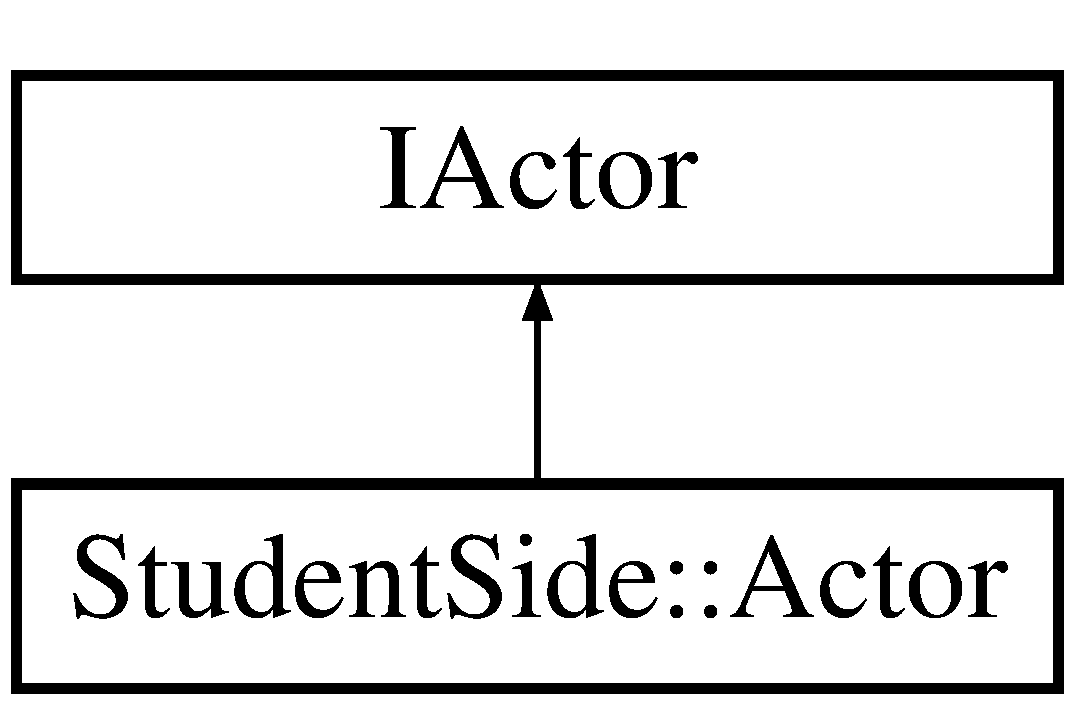
\includegraphics[height=2.000000cm]{class_student_side_1_1_actor}
\end{center}
\end{figure}
\subsection*{Public Member Functions}
\begin{DoxyCompactItemize}
\item 
\hyperlink{class_student_side_1_1_actor_a975c8c762266aaa7a77bd66fc4ec52f8}{Actor} ()
\begin{DoxyCompactList}\small\item\em Constructor for Actors. \end{DoxyCompactList}\item 
\hyperlink{class_student_side_1_1_actor_ae5f1f32ef2603cff6d9f91648ad723df}{$\sim$\-Actor} ()
\begin{DoxyCompactList}\small\item\em Destructor. \end{DoxyCompactList}\item 
Interface\-::\-Location \hyperlink{class_student_side_1_1_actor_a7da7be8bf80fd2cb6ecccb5643c5550b}{give\-Location} () const override
\begin{DoxyCompactList}\small\item\em give\-Location method gives location from Interface \end{DoxyCompactList}\item 
void \hyperlink{class_student_side_1_1_actor_ac3027790dbf5d48a783931a39876b16f}{move} (Interface\-::\-Location loc) override
\begin{DoxyCompactList}\small\item\em move the actor to wanted location \end{DoxyCompactList}\item 
bool \hyperlink{class_student_side_1_1_actor_ae43895e750efd94a11ed0377de1541a2}{is\-Removed} () const override
\begin{DoxyCompactList}\small\item\em is\-Removed checks if actor has been removed \end{DoxyCompactList}\item 
void \hyperlink{class_student_side_1_1_actor_ac5be31d931bf28cfd9044c991ea7ad18}{remove} () override
\begin{DoxyCompactList}\small\item\em remove actor \end{DoxyCompactList}\item 
void \hyperlink{class_student_side_1_1_actor_a9e2ebb8ad1118556222cb153e9a4cd3e}{add\-Location} (Interface\-::\-Location $\ast$location)
\begin{DoxyCompactList}\small\item\em add\-Location to actor \end{DoxyCompactList}\end{DoxyCompactItemize}


\subsection{Constructor \& Destructor Documentation}
\hypertarget{class_student_side_1_1_actor_a975c8c762266aaa7a77bd66fc4ec52f8}{\index{Student\-Side\-::\-Actor@{Student\-Side\-::\-Actor}!Actor@{Actor}}
\index{Actor@{Actor}!StudentSide::Actor@{Student\-Side\-::\-Actor}}
\subsubsection[{Actor}]{\setlength{\rightskip}{0pt plus 5cm}Student\-Side\-::\-Actor\-::\-Actor (
\begin{DoxyParamCaption}
{}
\end{DoxyParamCaption}
)}}\label{class_student_side_1_1_actor_a975c8c762266aaa7a77bd66fc4ec52f8}


Constructor for Actors. 

\begin{DoxyPrecond}{Precondition}
-\/ 
\end{DoxyPrecond}
\hypertarget{class_student_side_1_1_actor_ae5f1f32ef2603cff6d9f91648ad723df}{\index{Student\-Side\-::\-Actor@{Student\-Side\-::\-Actor}!$\sim$\-Actor@{$\sim$\-Actor}}
\index{$\sim$\-Actor@{$\sim$\-Actor}!StudentSide::Actor@{Student\-Side\-::\-Actor}}
\subsubsection[{$\sim$\-Actor}]{\setlength{\rightskip}{0pt plus 5cm}Student\-Side\-::\-Actor\-::$\sim$\-Actor (
\begin{DoxyParamCaption}
{}
\end{DoxyParamCaption}
)}}\label{class_student_side_1_1_actor_ae5f1f32ef2603cff6d9f91648ad723df}


Destructor. 

\begin{DoxyPrecond}{Precondition}
-\/ 
\end{DoxyPrecond}


\subsection{Member Function Documentation}
\hypertarget{class_student_side_1_1_actor_a9e2ebb8ad1118556222cb153e9a4cd3e}{\index{Student\-Side\-::\-Actor@{Student\-Side\-::\-Actor}!add\-Location@{add\-Location}}
\index{add\-Location@{add\-Location}!StudentSide::Actor@{Student\-Side\-::\-Actor}}
\subsubsection[{add\-Location}]{\setlength{\rightskip}{0pt plus 5cm}void Student\-Side\-::\-Actor\-::add\-Location (
\begin{DoxyParamCaption}
\item[{Interface\-::\-Location $\ast$}]{location}
\end{DoxyParamCaption}
)}}\label{class_student_side_1_1_actor_a9e2ebb8ad1118556222cb153e9a4cd3e}


add\-Location to actor 


\begin{DoxyParams}{Parameters}
{\em location} & of a actor \\
\hline
\end{DoxyParams}
\begin{DoxyPrecond}{Precondition}
-\/ 
\end{DoxyPrecond}
\begin{DoxyPostcond}{Postcondition}
Exception guarantee\-: Minimum 
\end{DoxyPostcond}
\hypertarget{class_student_side_1_1_actor_a7da7be8bf80fd2cb6ecccb5643c5550b}{\index{Student\-Side\-::\-Actor@{Student\-Side\-::\-Actor}!give\-Location@{give\-Location}}
\index{give\-Location@{give\-Location}!StudentSide::Actor@{Student\-Side\-::\-Actor}}
\subsubsection[{give\-Location}]{\setlength{\rightskip}{0pt plus 5cm}Interface\-::\-Location Student\-Side\-::\-Actor\-::give\-Location (
\begin{DoxyParamCaption}
{}
\end{DoxyParamCaption}
) const\hspace{0.3cm}{\ttfamily [override]}}}\label{class_student_side_1_1_actor_a7da7be8bf80fd2cb6ecccb5643c5550b}


give\-Location method gives location from Interface 

\begin{DoxyPrecond}{Precondition}
-\/ 
\end{DoxyPrecond}
\begin{DoxyPostcond}{Postcondition}
Exception guarantee\-: Strong 
\end{DoxyPostcond}
\begin{DoxyReturn}{Returns}
location of actor 
\end{DoxyReturn}
\hypertarget{class_student_side_1_1_actor_ae43895e750efd94a11ed0377de1541a2}{\index{Student\-Side\-::\-Actor@{Student\-Side\-::\-Actor}!is\-Removed@{is\-Removed}}
\index{is\-Removed@{is\-Removed}!StudentSide::Actor@{Student\-Side\-::\-Actor}}
\subsubsection[{is\-Removed}]{\setlength{\rightskip}{0pt plus 5cm}bool Student\-Side\-::\-Actor\-::is\-Removed (
\begin{DoxyParamCaption}
{}
\end{DoxyParamCaption}
) const\hspace{0.3cm}{\ttfamily [override]}}}\label{class_student_side_1_1_actor_ae43895e750efd94a11ed0377de1541a2}


is\-Removed checks if actor has been removed 

\begin{DoxyReturn}{Returns}
boolean value of if actor is removed 
\end{DoxyReturn}
\begin{DoxyPrecond}{Precondition}
-\/ 
\end{DoxyPrecond}
\begin{DoxyPostcond}{Postcondition}
Exception guarantee\-: Basic 
\end{DoxyPostcond}
\hypertarget{class_student_side_1_1_actor_ac3027790dbf5d48a783931a39876b16f}{\index{Student\-Side\-::\-Actor@{Student\-Side\-::\-Actor}!move@{move}}
\index{move@{move}!StudentSide::Actor@{Student\-Side\-::\-Actor}}
\subsubsection[{move}]{\setlength{\rightskip}{0pt plus 5cm}void Student\-Side\-::\-Actor\-::move (
\begin{DoxyParamCaption}
\item[{Interface\-::\-Location}]{loc}
\end{DoxyParamCaption}
)\hspace{0.3cm}{\ttfamily [override]}}}\label{class_student_side_1_1_actor_ac3027790dbf5d48a783931a39876b16f}


move the actor to wanted location 


\begin{DoxyParams}{Parameters}
{\em loc,location} & of the actor \\
\hline
\end{DoxyParams}
\begin{DoxyPrecond}{Precondition}
loc.\-x $>$ 0, loc.\-y $>$ 0, loc.\-x $<$ 1100, loc.\-y $<$ 590 
\end{DoxyPrecond}
\begin{DoxyPostcond}{Postcondition}
Exception guarantee\-: Strong 
\end{DoxyPostcond}
\hypertarget{class_student_side_1_1_actor_ac5be31d931bf28cfd9044c991ea7ad18}{\index{Student\-Side\-::\-Actor@{Student\-Side\-::\-Actor}!remove@{remove}}
\index{remove@{remove}!StudentSide::Actor@{Student\-Side\-::\-Actor}}
\subsubsection[{remove}]{\setlength{\rightskip}{0pt plus 5cm}void Student\-Side\-::\-Actor\-::remove (
\begin{DoxyParamCaption}
{}
\end{DoxyParamCaption}
)\hspace{0.3cm}{\ttfamily [override]}}}\label{class_student_side_1_1_actor_ac5be31d931bf28cfd9044c991ea7ad18}


remove actor 

\begin{DoxyPrecond}{Precondition}
-\/ 
\end{DoxyPrecond}
\begin{DoxyPostcond}{Postcondition}
Exception guarantee\-: nothrow 
\end{DoxyPostcond}


The documentation for this class was generated from the following files\-:\begin{DoxyCompactItemize}
\item 
Game/\hyperlink{actor_8hh}{actor.\-hh}\item 
Game/\hyperlink{actor_8cpp}{actor.\-cpp}\end{DoxyCompactItemize}

\hypertarget{class_student_side_1_1_actor_item}{\section{Student\-Side\-:\-:Actor\-Item Class Reference}
\label{class_student_side_1_1_actor_item}\index{Student\-Side\-::\-Actor\-Item@{Student\-Side\-::\-Actor\-Item}}
}


{\ttfamily \#include $<$actoritem.\-hh$>$}

Inheritance diagram for Student\-Side\-:\-:Actor\-Item\-:\begin{figure}[H]
\begin{center}
\leavevmode
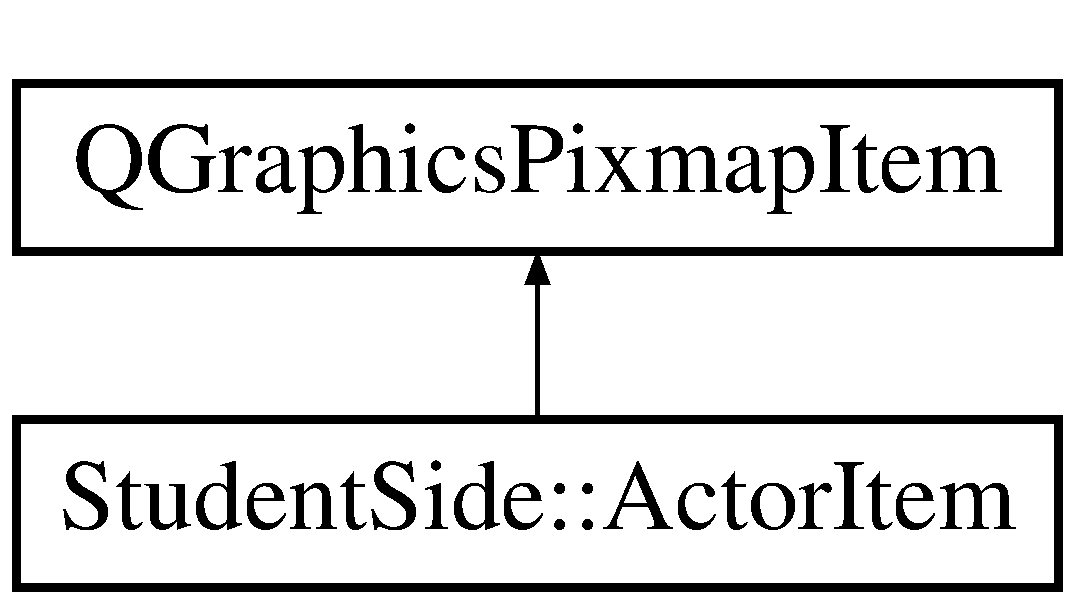
\includegraphics[height=2.000000cm]{class_student_side_1_1_actor_item}
\end{center}
\end{figure}
\subsection*{Public Member Functions}
\begin{DoxyCompactItemize}
\item 
\hyperlink{class_student_side_1_1_actor_item_a741d8a8d3413683146380fa1311e7ffa}{Actor\-Item} (int \hyperlink{jquery_8js_a4c3eadaa5164016d2c340d495fc6e55e}{x}, int y, int type=0)
\begin{DoxyCompactList}\small\item\em \hyperlink{class_student_side_1_1_actor_item}{Actor\-Item} constructor that sets the pictures for actors. \end{DoxyCompactList}\item 
\hyperlink{class_student_side_1_1_actor_item_a089e14fc439cd834bd8aec50cd55be87}{$\sim$\-Actor\-Item} ()
\begin{DoxyCompactList}\small\item\em Destructor. \end{DoxyCompactList}\item 
void \hyperlink{class_student_side_1_1_actor_item_a5a2f0d7ad57b6a71f24112682e46c9a3}{set\-Coord} (int \hyperlink{jquery_8js_a4c3eadaa5164016d2c340d495fc6e55e}{x}, int y)
\begin{DoxyCompactList}\small\item\em set\-Coord sets the actor\-Items position to the gameboard \end{DoxyCompactList}\end{DoxyCompactItemize}


\subsection{Constructor \& Destructor Documentation}
\hypertarget{class_student_side_1_1_actor_item_a741d8a8d3413683146380fa1311e7ffa}{\index{Student\-Side\-::\-Actor\-Item@{Student\-Side\-::\-Actor\-Item}!Actor\-Item@{Actor\-Item}}
\index{Actor\-Item@{Actor\-Item}!StudentSide::ActorItem@{Student\-Side\-::\-Actor\-Item}}
\subsubsection[{Actor\-Item}]{\setlength{\rightskip}{0pt plus 5cm}Student\-Side\-::\-Actor\-Item\-::\-Actor\-Item (
\begin{DoxyParamCaption}
\item[{int}]{x, }
\item[{int}]{y, }
\item[{int}]{type = {\ttfamily 0}}
\end{DoxyParamCaption}
)}}\label{class_student_side_1_1_actor_item_a741d8a8d3413683146380fa1311e7ffa}


\hyperlink{class_student_side_1_1_actor_item}{Actor\-Item} constructor that sets the pictures for actors. 


\begin{DoxyParams}{Parameters}
{\em x} & x-\/coordinate \\
\hline
{\em y} & y-\/coordinate \\
\hline
{\em type} & actor type \\
\hline
\end{DoxyParams}
\begin{DoxyPrecond}{Precondition}
coordinates must be in range of map coordinates. 
\end{DoxyPrecond}
\begin{DoxyPostcond}{Postcondition}
Exception guaranteed\-: nothrow 
\end{DoxyPostcond}
\hypertarget{class_student_side_1_1_actor_item_a089e14fc439cd834bd8aec50cd55be87}{\index{Student\-Side\-::\-Actor\-Item@{Student\-Side\-::\-Actor\-Item}!$\sim$\-Actor\-Item@{$\sim$\-Actor\-Item}}
\index{$\sim$\-Actor\-Item@{$\sim$\-Actor\-Item}!StudentSide::ActorItem@{Student\-Side\-::\-Actor\-Item}}
\subsubsection[{$\sim$\-Actor\-Item}]{\setlength{\rightskip}{0pt plus 5cm}Student\-Side\-::\-Actor\-Item\-::$\sim$\-Actor\-Item (
\begin{DoxyParamCaption}
{}
\end{DoxyParamCaption}
)}}\label{class_student_side_1_1_actor_item_a089e14fc439cd834bd8aec50cd55be87}


Destructor. 

\begin{DoxyPostcond}{Postcondition}
Exception guaranteed\-: nothrow 
\end{DoxyPostcond}


\subsection{Member Function Documentation}
\hypertarget{class_student_side_1_1_actor_item_a5a2f0d7ad57b6a71f24112682e46c9a3}{\index{Student\-Side\-::\-Actor\-Item@{Student\-Side\-::\-Actor\-Item}!set\-Coord@{set\-Coord}}
\index{set\-Coord@{set\-Coord}!StudentSide::ActorItem@{Student\-Side\-::\-Actor\-Item}}
\subsubsection[{set\-Coord}]{\setlength{\rightskip}{0pt plus 5cm}void Student\-Side\-::\-Actor\-Item\-::set\-Coord (
\begin{DoxyParamCaption}
\item[{int}]{x, }
\item[{int}]{y}
\end{DoxyParamCaption}
)}}\label{class_student_side_1_1_actor_item_a5a2f0d7ad57b6a71f24112682e46c9a3}


set\-Coord sets the actor\-Items position to the gameboard 


\begin{DoxyParams}{Parameters}
{\em x} & x-\/coordination \\
\hline
{\em y} & y-\/coordination \\
\hline
\end{DoxyParams}
\begin{DoxyPrecond}{Precondition}
-\/ 
\end{DoxyPrecond}
\begin{DoxyPostcond}{Postcondition}
Exception guaranteed\-: minimum 
\end{DoxyPostcond}


The documentation for this class was generated from the following files\-:\begin{DoxyCompactItemize}
\item 
Game/\hyperlink{actoritem_8hh}{actoritem.\-hh}\item 
Game/\hyperlink{actoritem_8cpp}{actoritem.\-cpp}\end{DoxyCompactItemize}

\hypertarget{class_student_side_1_1_city}{\section{Student\-Side\-:\-:City Class Reference}
\label{class_student_side_1_1_city}\index{Student\-Side\-::\-City@{Student\-Side\-::\-City}}
}


The \hyperlink{class_student_side_1_1_city}{City} class that defines city operations.  




{\ttfamily \#include $<$city.\-hh$>$}

Inheritance diagram for Student\-Side\-:\-:City\-:\begin{figure}[H]
\begin{center}
\leavevmode
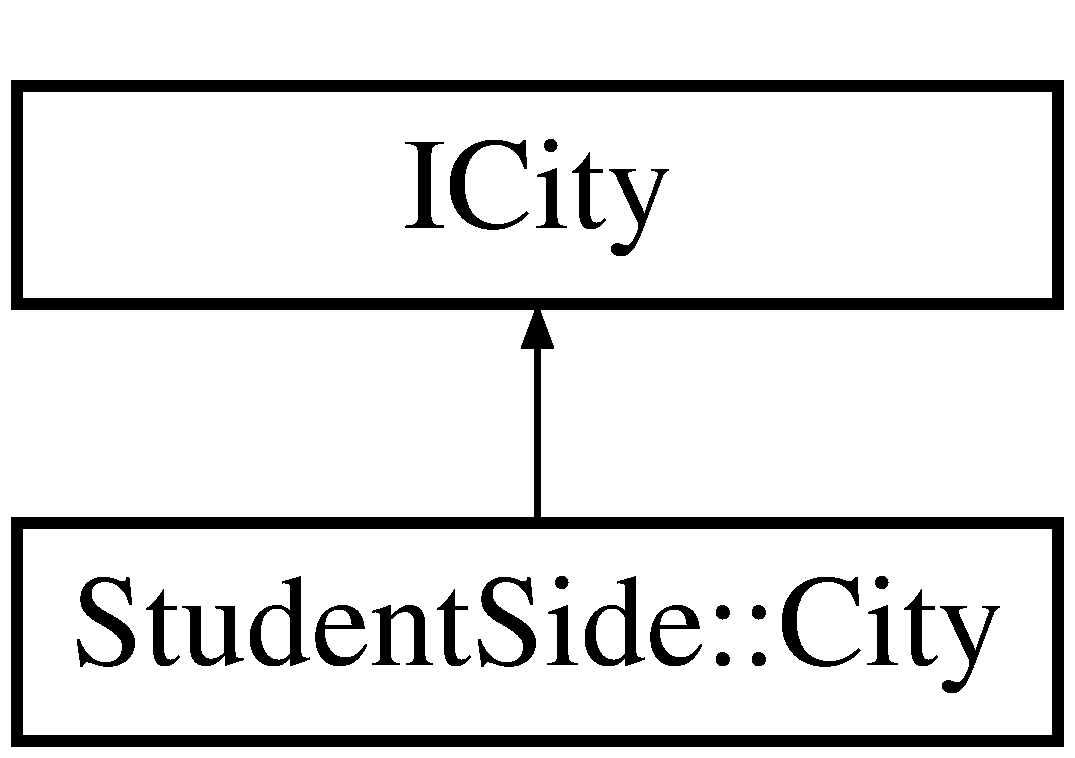
\includegraphics[height=2.000000cm]{class_student_side_1_1_city}
\end{center}
\end{figure}
\subsection*{Public Member Functions}
\begin{DoxyCompactItemize}
\item 
\hyperlink{class_student_side_1_1_city_ad5a0fd2a6e60fbd54bf0dfef0d5f849a}{City} ()
\begin{DoxyCompactList}\small\item\em \hyperlink{class_student_side_1_1_city}{City} constructor. \end{DoxyCompactList}\item 
\hyperlink{class_student_side_1_1_city_a9e98110785506a88ac9847755459988d}{$\sim$\-City} ()
\begin{DoxyCompactList}\small\item\em Destructor. \end{DoxyCompactList}\item 
void \hyperlink{class_student_side_1_1_city_a04accbc4ff8e507bc9b8cedae2444183}{set\-Background} (Q\-Image \&basicbackground, Q\-Image \&bigbackground) override
\begin{DoxyCompactList}\small\item\em set\-Background sets the map picture to game board. \end{DoxyCompactList}\item 
void \hyperlink{class_student_side_1_1_city_a7f57965f914ed8f3c544ce1324ba4fe8}{set\-Clock} (Q\-Time clock) override
\begin{DoxyCompactList}\small\item\em set\-Clock sets the time of a game clock. \end{DoxyCompactList}\item 
void \hyperlink{class_student_side_1_1_city_a54f4d302402630182a705d902c8e346a}{add\-Stop} (std\-::shared\-\_\-ptr$<$ Interface\-::\-I\-Stop $>$ stop) override
\begin{DoxyCompactList}\small\item\em add\-Stop adds a stop to the city. \end{DoxyCompactList}\item 
void \hyperlink{class_student_side_1_1_city_a10c22f1803f70837638d1f5543eb9627}{start\-Game} () override
\begin{DoxyCompactList}\small\item\em start\-Game changes game state to gamestate from initstate. \end{DoxyCompactList}\item 
void \hyperlink{class_student_side_1_1_city_af3c2bc7c60238c935c42b66e6f8d257a}{add\-Actor} (std\-::shared\-\_\-ptr$<$ Interface\-::\-I\-Actor $>$ newactor) override
\begin{DoxyCompactList}\small\item\em add\-Actor adds a new actor to the city. \end{DoxyCompactList}\item 
void \hyperlink{class_student_side_1_1_city_ae3065589fed9daf61c01978e013bdd13}{remove\-Actor} (std\-::shared\-\_\-ptr$<$ Interface\-::\-I\-Actor $>$ actor) override
\begin{DoxyCompactList}\small\item\em remove\-Actor removes the actor from the city. \end{DoxyCompactList}\item 
void \hyperlink{class_student_side_1_1_city_aa4b2cda0950f77412551403669cafd00}{actor\-Removed} (std\-::shared\-\_\-ptr$<$ Interface\-::\-I\-Actor $>$ actor) override
\begin{DoxyCompactList}\small\item\em actor\-Removed tells the city that actor is removed. \end{DoxyCompactList}\item 
bool \hyperlink{class_student_side_1_1_city_aee72420052d9af04957551474c1f7af9}{find\-Actor} (std\-::shared\-\_\-ptr$<$ Interface\-::\-I\-Actor $>$ actor) const override
\begin{DoxyCompactList}\small\item\em find\-Actor try to find if actor can be found in the city. \end{DoxyCompactList}\item 
std\-::vector$<$ std\-::shared\-\_\-ptr\\*
$<$ Interface\-::\-I\-Actor $>$ $>$ \hyperlink{class_student_side_1_1_city_a2285ee28fb606dd774b8e60979d6e820}{get\-Nearby\-Actors} (Interface\-::\-Location loc) const override
\begin{DoxyCompactList}\small\item\em get\-Nearby\-Actors returns vector containing actors that are close to given position. \end{DoxyCompactList}\item 
void \hyperlink{class_student_side_1_1_city_ae74783e6701ceb40dd9efbd3faf3e1c3}{actor\-Moved} (std\-::shared\-\_\-ptr$<$ Interface\-::\-I\-Actor $>$ actor) override
\begin{DoxyCompactList}\small\item\em actor\-Moved tells if actor is being moved \end{DoxyCompactList}\item 
bool \hyperlink{class_student_side_1_1_city_a9ca889641234d84e92fa97b999ae1ee4}{is\-Game\-Over} () const override
\begin{DoxyCompactList}\small\item\em is\-Game\-Over tells if game ends. \end{DoxyCompactList}\item 
Q\-Image \hyperlink{class_student_side_1_1_city_ab3ac8687f8213b2a26484214a7925dc2}{get\-Image} (std\-::string image\-\_\-size)
\begin{DoxyCompactList}\small\item\em get\-Image returns the image depending on wanted size. \end{DoxyCompactList}\item 
void \hyperlink{class_student_side_1_1_city_a5d7dffa807359354d94bd031fb207767}{add\-Ui} (std\-::shared\-\_\-ptr$<$ \hyperlink{class_student_side_1_1_mainwindow}{Student\-Side\-::\-Mainwindow} $>$ ui)
\begin{DoxyCompactList}\small\item\em add\-Ui adds mainwindows userinterface to city. \end{DoxyCompactList}\item 
void \hyperlink{class_student_side_1_1_city_a9e77dd00ce37d3467bb078d0fb7b3cca}{make\-Player} ()
\begin{DoxyCompactList}\small\item\em make\-Player creates player and adds it to userinterface. \end{DoxyCompactList}\item 
void \hyperlink{class_student_side_1_1_city_a3f0375a49769a2a3456853a354732efe}{Destroy\-Timo} (std\-::shared\-\_\-ptr$<$ Interface\-::\-I\-Actor $>$ actor)
\item 
std\-::vector$<$ std\-::shared\-\_\-ptr\\*
$<$ Interface\-::\-I\-Actor $>$ $>$ \hyperlink{class_student_side_1_1_city_ab12fa6213daf693fc5602317c04c363c}{give\-Moved\-Actors} ()
\begin{DoxyCompactList}\small\item\em give\-Moved\-Actors returns vector containing moved actors. \end{DoxyCompactList}\item 
std\-::vector$<$ std\-::shared\-\_\-ptr\\*
$<$ Interface\-::\-I\-Actor $>$ $>$ \hyperlink{class_student_side_1_1_city_a2e0283747d6ad3d03b445d9def9780cb}{give\-New\-Passengers} ()
\item 
void \hyperlink{class_student_side_1_1_city_a4030f4a976670a9d33b990f2c7d1f11c}{take\-Stats} (std\-::shared\-\_\-ptr$<$ \hyperlink{class_student_side_1_1_statistics}{Student\-Side\-::\-Statistics} $>$ stats)
\item 
void \hyperlink{class_student_side_1_1_city_a8daa819e3acf9ce4c7a51e2dd6d53895}{add\-Nuke} ()
\item 
void \hyperlink{class_student_side_1_1_city_af81fc684dc3cdc743d8a267e0de37f7b}{nuke\-City} ()
\end{DoxyCompactItemize}


\subsection{Detailed Description}
The \hyperlink{class_student_side_1_1_city}{City} class that defines city operations. 

\subsection{Constructor \& Destructor Documentation}
\hypertarget{class_student_side_1_1_city_ad5a0fd2a6e60fbd54bf0dfef0d5f849a}{\index{Student\-Side\-::\-City@{Student\-Side\-::\-City}!City@{City}}
\index{City@{City}!StudentSide::City@{Student\-Side\-::\-City}}
\subsubsection[{City}]{\setlength{\rightskip}{0pt plus 5cm}Student\-Side\-::\-City\-::\-City (
\begin{DoxyParamCaption}
{}
\end{DoxyParamCaption}
)}}\label{class_student_side_1_1_city_ad5a0fd2a6e60fbd54bf0dfef0d5f849a}


\hyperlink{class_student_side_1_1_city}{City} constructor. 

\hypertarget{class_student_side_1_1_city_a9e98110785506a88ac9847755459988d}{\index{Student\-Side\-::\-City@{Student\-Side\-::\-City}!$\sim$\-City@{$\sim$\-City}}
\index{$\sim$\-City@{$\sim$\-City}!StudentSide::City@{Student\-Side\-::\-City}}
\subsubsection[{$\sim$\-City}]{\setlength{\rightskip}{0pt plus 5cm}Student\-Side\-::\-City\-::$\sim$\-City (
\begin{DoxyParamCaption}
{}
\end{DoxyParamCaption}
)}}\label{class_student_side_1_1_city_a9e98110785506a88ac9847755459988d}


Destructor. 



\subsection{Member Function Documentation}
\hypertarget{class_student_side_1_1_city_ae74783e6701ceb40dd9efbd3faf3e1c3}{\index{Student\-Side\-::\-City@{Student\-Side\-::\-City}!actor\-Moved@{actor\-Moved}}
\index{actor\-Moved@{actor\-Moved}!StudentSide::City@{Student\-Side\-::\-City}}
\subsubsection[{actor\-Moved}]{\setlength{\rightskip}{0pt plus 5cm}void Student\-Side\-::\-City\-::actor\-Moved (
\begin{DoxyParamCaption}
\item[{std\-::shared\-\_\-ptr$<$ Interface\-::\-I\-Actor $>$}]{actor}
\end{DoxyParamCaption}
)\hspace{0.3cm}{\ttfamily [override]}}}\label{class_student_side_1_1_city_ae74783e6701ceb40dd9efbd3faf3e1c3}


actor\-Moved tells if actor is being moved 


\begin{DoxyParams}{Parameters}
{\em actor} & \hyperlink{class_student_side_1_1_actor}{Actor} that has moved. \\
\hline
\end{DoxyParams}
\hypertarget{class_student_side_1_1_city_aa4b2cda0950f77412551403669cafd00}{\index{Student\-Side\-::\-City@{Student\-Side\-::\-City}!actor\-Removed@{actor\-Removed}}
\index{actor\-Removed@{actor\-Removed}!StudentSide::City@{Student\-Side\-::\-City}}
\subsubsection[{actor\-Removed}]{\setlength{\rightskip}{0pt plus 5cm}void Student\-Side\-::\-City\-::actor\-Removed (
\begin{DoxyParamCaption}
\item[{std\-::shared\-\_\-ptr$<$ Interface\-::\-I\-Actor $>$}]{actor}
\end{DoxyParamCaption}
)\hspace{0.3cm}{\ttfamily [override]}}}\label{class_student_side_1_1_city_aa4b2cda0950f77412551403669cafd00}


actor\-Removed tells the city that actor is removed. 


\begin{DoxyParams}{Parameters}
{\em actor} & \hyperlink{class_student_side_1_1_actor}{Actor} that is set removed ingame. \\
\hline
\end{DoxyParams}
\hypertarget{class_student_side_1_1_city_af3c2bc7c60238c935c42b66e6f8d257a}{\index{Student\-Side\-::\-City@{Student\-Side\-::\-City}!add\-Actor@{add\-Actor}}
\index{add\-Actor@{add\-Actor}!StudentSide::City@{Student\-Side\-::\-City}}
\subsubsection[{add\-Actor}]{\setlength{\rightskip}{0pt plus 5cm}void Student\-Side\-::\-City\-::add\-Actor (
\begin{DoxyParamCaption}
\item[{std\-::shared\-\_\-ptr$<$ Interface\-::\-I\-Actor $>$}]{newactor}
\end{DoxyParamCaption}
)\hspace{0.3cm}{\ttfamily [override]}}}\label{class_student_side_1_1_city_af3c2bc7c60238c935c42b66e6f8d257a}


add\-Actor adds a new actor to the city. 


\begin{DoxyParams}{Parameters}
{\em newactor} & actor to be added to the city. \\
\hline
\end{DoxyParams}
\hypertarget{class_student_side_1_1_city_a8daa819e3acf9ce4c7a51e2dd6d53895}{\index{Student\-Side\-::\-City@{Student\-Side\-::\-City}!add\-Nuke@{add\-Nuke}}
\index{add\-Nuke@{add\-Nuke}!StudentSide::City@{Student\-Side\-::\-City}}
\subsubsection[{add\-Nuke}]{\setlength{\rightskip}{0pt plus 5cm}void Student\-Side\-::\-City\-::add\-Nuke (
\begin{DoxyParamCaption}
{}
\end{DoxyParamCaption}
)}}\label{class_student_side_1_1_city_a8daa819e3acf9ce4c7a51e2dd6d53895}
\hypertarget{class_student_side_1_1_city_a54f4d302402630182a705d902c8e346a}{\index{Student\-Side\-::\-City@{Student\-Side\-::\-City}!add\-Stop@{add\-Stop}}
\index{add\-Stop@{add\-Stop}!StudentSide::City@{Student\-Side\-::\-City}}
\subsubsection[{add\-Stop}]{\setlength{\rightskip}{0pt plus 5cm}void Student\-Side\-::\-City\-::add\-Stop (
\begin{DoxyParamCaption}
\item[{std\-::shared\-\_\-ptr$<$ Interface\-::\-I\-Stop $>$}]{stop}
\end{DoxyParamCaption}
)\hspace{0.3cm}{\ttfamily [override]}}}\label{class_student_side_1_1_city_a54f4d302402630182a705d902c8e346a}


add\-Stop adds a stop to the city. 


\begin{DoxyParams}{Parameters}
{\em stop} & pointer to a stop object. \\
\hline
\end{DoxyParams}
\hypertarget{class_student_side_1_1_city_a5d7dffa807359354d94bd031fb207767}{\index{Student\-Side\-::\-City@{Student\-Side\-::\-City}!add\-Ui@{add\-Ui}}
\index{add\-Ui@{add\-Ui}!StudentSide::City@{Student\-Side\-::\-City}}
\subsubsection[{add\-Ui}]{\setlength{\rightskip}{0pt plus 5cm}void Student\-Side\-::\-City\-::add\-Ui (
\begin{DoxyParamCaption}
\item[{std\-::shared\-\_\-ptr$<$ {\bf Student\-Side\-::\-Mainwindow} $>$}]{ui}
\end{DoxyParamCaption}
)}}\label{class_student_side_1_1_city_a5d7dffa807359354d94bd031fb207767}


add\-Ui adds mainwindows userinterface to city. 


\begin{DoxyParams}{Parameters}
{\em ui} & Userinterface. \\
\hline
\end{DoxyParams}
\hypertarget{class_student_side_1_1_city_a3f0375a49769a2a3456853a354732efe}{\index{Student\-Side\-::\-City@{Student\-Side\-::\-City}!Destroy\-Timo@{Destroy\-Timo}}
\index{Destroy\-Timo@{Destroy\-Timo}!StudentSide::City@{Student\-Side\-::\-City}}
\subsubsection[{Destroy\-Timo}]{\setlength{\rightskip}{0pt plus 5cm}void Student\-Side\-::\-City\-::\-Destroy\-Timo (
\begin{DoxyParamCaption}
\item[{std\-::shared\-\_\-ptr$<$ Interface\-::\-I\-Actor $>$}]{actor}
\end{DoxyParamCaption}
)}}\label{class_student_side_1_1_city_a3f0375a49769a2a3456853a354732efe}
\hypertarget{class_student_side_1_1_city_aee72420052d9af04957551474c1f7af9}{\index{Student\-Side\-::\-City@{Student\-Side\-::\-City}!find\-Actor@{find\-Actor}}
\index{find\-Actor@{find\-Actor}!StudentSide::City@{Student\-Side\-::\-City}}
\subsubsection[{find\-Actor}]{\setlength{\rightskip}{0pt plus 5cm}bool Student\-Side\-::\-City\-::find\-Actor (
\begin{DoxyParamCaption}
\item[{std\-::shared\-\_\-ptr$<$ Interface\-::\-I\-Actor $>$}]{actor}
\end{DoxyParamCaption}
) const\hspace{0.3cm}{\ttfamily [override]}}}\label{class_student_side_1_1_city_aee72420052d9af04957551474c1f7af9}


find\-Actor try to find if actor can be found in the city. 


\begin{DoxyParams}{Parameters}
{\em actor} & \hyperlink{class_student_side_1_1_actor}{Actor} that is looked from city. \\
\hline
\end{DoxyParams}
\begin{DoxyReturn}{Returns}
Boolean value that tells if actor can be found. 
\end{DoxyReturn}
\hypertarget{class_student_side_1_1_city_ab3ac8687f8213b2a26484214a7925dc2}{\index{Student\-Side\-::\-City@{Student\-Side\-::\-City}!get\-Image@{get\-Image}}
\index{get\-Image@{get\-Image}!StudentSide::City@{Student\-Side\-::\-City}}
\subsubsection[{get\-Image}]{\setlength{\rightskip}{0pt plus 5cm}Q\-Image Student\-Side\-::\-City\-::get\-Image (
\begin{DoxyParamCaption}
\item[{std\-::string}]{image\-\_\-size}
\end{DoxyParamCaption}
)}}\label{class_student_side_1_1_city_ab3ac8687f8213b2a26484214a7925dc2}


get\-Image returns the image depending on wanted size. 


\begin{DoxyParams}{Parameters}
{\em image\-\_\-size} & Size of the wanted image used. \\
\hline
\end{DoxyParams}
\begin{DoxyReturn}{Returns}
returns wanted image of map. 
\end{DoxyReturn}
\hypertarget{class_student_side_1_1_city_a2285ee28fb606dd774b8e60979d6e820}{\index{Student\-Side\-::\-City@{Student\-Side\-::\-City}!get\-Nearby\-Actors@{get\-Nearby\-Actors}}
\index{get\-Nearby\-Actors@{get\-Nearby\-Actors}!StudentSide::City@{Student\-Side\-::\-City}}
\subsubsection[{get\-Nearby\-Actors}]{\setlength{\rightskip}{0pt plus 5cm}std\-::vector$<$ std\-::shared\-\_\-ptr$<$ Interface\-::\-I\-Actor $>$ $>$ Student\-Side\-::\-City\-::get\-Nearby\-Actors (
\begin{DoxyParamCaption}
\item[{Interface\-::\-Location}]{loc}
\end{DoxyParamCaption}
) const\hspace{0.3cm}{\ttfamily [override]}}}\label{class_student_side_1_1_city_a2285ee28fb606dd774b8e60979d6e820}


get\-Nearby\-Actors returns vector containing actors that are close to given position. 


\begin{DoxyParams}{Parameters}
{\em loc} & Location for getting the actors close to it. \\
\hline
\end{DoxyParams}
\begin{DoxyReturn}{Returns}
Vector of actors. 
\end{DoxyReturn}
\hypertarget{class_student_side_1_1_city_ab12fa6213daf693fc5602317c04c363c}{\index{Student\-Side\-::\-City@{Student\-Side\-::\-City}!give\-Moved\-Actors@{give\-Moved\-Actors}}
\index{give\-Moved\-Actors@{give\-Moved\-Actors}!StudentSide::City@{Student\-Side\-::\-City}}
\subsubsection[{give\-Moved\-Actors}]{\setlength{\rightskip}{0pt plus 5cm}std\-::vector$<$ std\-::shared\-\_\-ptr$<$ Interface\-::\-I\-Actor $>$ $>$ Student\-Side\-::\-City\-::give\-Moved\-Actors (
\begin{DoxyParamCaption}
{}
\end{DoxyParamCaption}
)}}\label{class_student_side_1_1_city_ab12fa6213daf693fc5602317c04c363c}


give\-Moved\-Actors returns vector containing moved actors. 

\begin{DoxyReturn}{Returns}
vector containing pointer to actors. 
\end{DoxyReturn}
\hypertarget{class_student_side_1_1_city_a2e0283747d6ad3d03b445d9def9780cb}{\index{Student\-Side\-::\-City@{Student\-Side\-::\-City}!give\-New\-Passengers@{give\-New\-Passengers}}
\index{give\-New\-Passengers@{give\-New\-Passengers}!StudentSide::City@{Student\-Side\-::\-City}}
\subsubsection[{give\-New\-Passengers}]{\setlength{\rightskip}{0pt plus 5cm}std\-::vector$<$ std\-::shared\-\_\-ptr$<$ Interface\-::\-I\-Actor $>$ $>$ Student\-Side\-::\-City\-::give\-New\-Passengers (
\begin{DoxyParamCaption}
{}
\end{DoxyParamCaption}
)}}\label{class_student_side_1_1_city_a2e0283747d6ad3d03b445d9def9780cb}
\hypertarget{class_student_side_1_1_city_a9ca889641234d84e92fa97b999ae1ee4}{\index{Student\-Side\-::\-City@{Student\-Side\-::\-City}!is\-Game\-Over@{is\-Game\-Over}}
\index{is\-Game\-Over@{is\-Game\-Over}!StudentSide::City@{Student\-Side\-::\-City}}
\subsubsection[{is\-Game\-Over}]{\setlength{\rightskip}{0pt plus 5cm}bool Student\-Side\-::\-City\-::is\-Game\-Over (
\begin{DoxyParamCaption}
{}
\end{DoxyParamCaption}
) const\hspace{0.3cm}{\ttfamily [override]}}}\label{class_student_side_1_1_city_a9ca889641234d84e92fa97b999ae1ee4}


is\-Game\-Over tells if game ends. 

\begin{DoxyReturn}{Returns}
Boolean value if game is over. 
\end{DoxyReturn}
\hypertarget{class_student_side_1_1_city_a9e77dd00ce37d3467bb078d0fb7b3cca}{\index{Student\-Side\-::\-City@{Student\-Side\-::\-City}!make\-Player@{make\-Player}}
\index{make\-Player@{make\-Player}!StudentSide::City@{Student\-Side\-::\-City}}
\subsubsection[{make\-Player}]{\setlength{\rightskip}{0pt plus 5cm}void Student\-Side\-::\-City\-::make\-Player (
\begin{DoxyParamCaption}
{}
\end{DoxyParamCaption}
)}}\label{class_student_side_1_1_city_a9e77dd00ce37d3467bb078d0fb7b3cca}


make\-Player creates player and adds it to userinterface. 

\hypertarget{class_student_side_1_1_city_af81fc684dc3cdc743d8a267e0de37f7b}{\index{Student\-Side\-::\-City@{Student\-Side\-::\-City}!nuke\-City@{nuke\-City}}
\index{nuke\-City@{nuke\-City}!StudentSide::City@{Student\-Side\-::\-City}}
\subsubsection[{nuke\-City}]{\setlength{\rightskip}{0pt plus 5cm}void Student\-Side\-::\-City\-::nuke\-City (
\begin{DoxyParamCaption}
{}
\end{DoxyParamCaption}
)}}\label{class_student_side_1_1_city_af81fc684dc3cdc743d8a267e0de37f7b}
\hypertarget{class_student_side_1_1_city_ae3065589fed9daf61c01978e013bdd13}{\index{Student\-Side\-::\-City@{Student\-Side\-::\-City}!remove\-Actor@{remove\-Actor}}
\index{remove\-Actor@{remove\-Actor}!StudentSide::City@{Student\-Side\-::\-City}}
\subsubsection[{remove\-Actor}]{\setlength{\rightskip}{0pt plus 5cm}void Student\-Side\-::\-City\-::remove\-Actor (
\begin{DoxyParamCaption}
\item[{std\-::shared\-\_\-ptr$<$ Interface\-::\-I\-Actor $>$}]{actor}
\end{DoxyParamCaption}
)\hspace{0.3cm}{\ttfamily [override]}}}\label{class_student_side_1_1_city_ae3065589fed9daf61c01978e013bdd13}


remove\-Actor removes the actor from the city. 


\begin{DoxyParams}{Parameters}
{\em actor} & \hyperlink{class_student_side_1_1_actor}{Actor} to be removed. \\
\hline
\end{DoxyParams}
\hypertarget{class_student_side_1_1_city_a04accbc4ff8e507bc9b8cedae2444183}{\index{Student\-Side\-::\-City@{Student\-Side\-::\-City}!set\-Background@{set\-Background}}
\index{set\-Background@{set\-Background}!StudentSide::City@{Student\-Side\-::\-City}}
\subsubsection[{set\-Background}]{\setlength{\rightskip}{0pt plus 5cm}void Student\-Side\-::\-City\-::set\-Background (
\begin{DoxyParamCaption}
\item[{Q\-Image \&}]{basicbackground, }
\item[{Q\-Image \&}]{bigbackground}
\end{DoxyParamCaption}
)\hspace{0.3cm}{\ttfamily [override]}}}\label{class_student_side_1_1_city_a04accbc4ff8e507bc9b8cedae2444183}


set\-Background sets the map picture to game board. 


\begin{DoxyParams}{Parameters}
{\em basicbackground} & Normal sised map. \\
\hline
{\em bigbackground} & Big sized map. Used if doing scrolling map-\/expansion. \\
\hline
\end{DoxyParams}
\hypertarget{class_student_side_1_1_city_a7f57965f914ed8f3c544ce1324ba4fe8}{\index{Student\-Side\-::\-City@{Student\-Side\-::\-City}!set\-Clock@{set\-Clock}}
\index{set\-Clock@{set\-Clock}!StudentSide::City@{Student\-Side\-::\-City}}
\subsubsection[{set\-Clock}]{\setlength{\rightskip}{0pt plus 5cm}void Student\-Side\-::\-City\-::set\-Clock (
\begin{DoxyParamCaption}
\item[{Q\-Time}]{clock}
\end{DoxyParamCaption}
)\hspace{0.3cm}{\ttfamily [override]}}}\label{class_student_side_1_1_city_a7f57965f914ed8f3c544ce1324ba4fe8}


set\-Clock sets the time of a game clock. 


\begin{DoxyParams}{Parameters}
{\em clock} & Game clock time at the function call. \\
\hline
\end{DoxyParams}
\hypertarget{class_student_side_1_1_city_a10c22f1803f70837638d1f5543eb9627}{\index{Student\-Side\-::\-City@{Student\-Side\-::\-City}!start\-Game@{start\-Game}}
\index{start\-Game@{start\-Game}!StudentSide::City@{Student\-Side\-::\-City}}
\subsubsection[{start\-Game}]{\setlength{\rightskip}{0pt plus 5cm}void Student\-Side\-::\-City\-::start\-Game (
\begin{DoxyParamCaption}
{}
\end{DoxyParamCaption}
)\hspace{0.3cm}{\ttfamily [override]}}}\label{class_student_side_1_1_city_a10c22f1803f70837638d1f5543eb9627}


start\-Game changes game state to gamestate from initstate. 

\hypertarget{class_student_side_1_1_city_a4030f4a976670a9d33b990f2c7d1f11c}{\index{Student\-Side\-::\-City@{Student\-Side\-::\-City}!take\-Stats@{take\-Stats}}
\index{take\-Stats@{take\-Stats}!StudentSide::City@{Student\-Side\-::\-City}}
\subsubsection[{take\-Stats}]{\setlength{\rightskip}{0pt plus 5cm}void Student\-Side\-::\-City\-::take\-Stats (
\begin{DoxyParamCaption}
\item[{std\-::shared\-\_\-ptr$<$ {\bf Student\-Side\-::\-Statistics} $>$}]{stats}
\end{DoxyParamCaption}
)}}\label{class_student_side_1_1_city_a4030f4a976670a9d33b990f2c7d1f11c}


The documentation for this class was generated from the following files\-:\begin{DoxyCompactItemize}
\item 
\hyperlink{city_8hh}{city.\-hh}\item 
\hyperlink{city_8cpp}{city.\-cpp}\end{DoxyCompactItemize}

\hypertarget{class_student_side_1_1_dialog_game_settings}{\section{Student\-Side\-:\-:Dialog\-Game\-Settings Class Reference}
\label{class_student_side_1_1_dialog_game_settings}\index{Student\-Side\-::\-Dialog\-Game\-Settings@{Student\-Side\-::\-Dialog\-Game\-Settings}}
}


The Dialog\-Gane\-Settings class sets up dialog window to get pre settings for the main game.  




{\ttfamily \#include $<$dialoggamesettings.\-hh$>$}

Inheritance diagram for Student\-Side\-:\-:Dialog\-Game\-Settings\-:\begin{figure}[H]
\begin{center}
\leavevmode
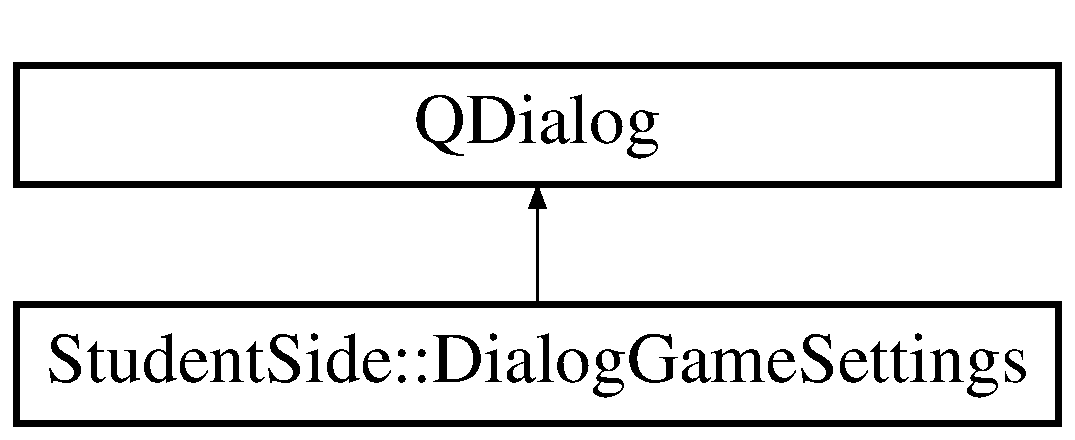
\includegraphics[height=2.000000cm]{class_student_side_1_1_dialog_game_settings}
\end{center}
\end{figure}
\subsection*{Public Slots}
\begin{DoxyCompactItemize}
\item 
void \hyperlink{class_student_side_1_1_dialog_game_settings_a9ee703736f4cde7137c785f00b0bc4d9}{normal} ()
\begin{DoxyCompactList}\small\item\em normal game \end{DoxyCompactList}\item 
void \hyperlink{class_student_side_1_1_dialog_game_settings_adce8f9e27b998911d35526350932c95a}{infinite} ()
\begin{DoxyCompactList}\small\item\em infinite time game \end{DoxyCompactList}\item 
void \hyperlink{class_student_side_1_1_dialog_game_settings_a1af75c606fddb4f29189c5cb65a4aa32}{set\-State1min} ()
\begin{DoxyCompactList}\small\item\em set\-State1min changes state of checkbox1min \end{DoxyCompactList}\item 
void \hyperlink{class_student_side_1_1_dialog_game_settings_ad8ddebcb7566ee6ee9abe7463659ce0b}{set\-State2min} ()
\begin{DoxyCompactList}\small\item\em set\-State2minc hanges state of checkbox2min \end{DoxyCompactList}\end{DoxyCompactItemize}
\subsection*{Signals}
\begin{DoxyCompactItemize}
\item 
void \hyperlink{class_student_side_1_1_dialog_game_settings_a17dedd787d5e757bcf6ac098e91938ed}{normal\-Settings} (Q\-String name, int timelimit)
\begin{DoxyCompactList}\small\item\em normal\-Settings to set normal game settings \end{DoxyCompactList}\item 
void \hyperlink{class_student_side_1_1_dialog_game_settings_ae6867086738b0a74b518d9683539dbe8}{infinite\-Settings} (Q\-String name)
\begin{DoxyCompactList}\small\item\em infinite\-Settings to set infinite time game. \end{DoxyCompactList}\end{DoxyCompactItemize}
\subsection*{Public Member Functions}
\begin{DoxyCompactItemize}
\item 
\hyperlink{class_student_side_1_1_dialog_game_settings_a862ee1ef85f8343eddc675b6737b3a39}{Dialog\-Game\-Settings} (Q\-Widget $\ast$parent=nullptr)
\begin{DoxyCompactList}\small\item\em \hyperlink{class_student_side_1_1_dialog_game_settings}{Dialog\-Game\-Settings} constructor for the dialog window. \end{DoxyCompactList}\item 
\hyperlink{class_student_side_1_1_dialog_game_settings_a1830c64fa4518461ce233aaff1674107}{$\sim$\-Dialog\-Game\-Settings} ()
\begin{DoxyCompactList}\small\item\em Destructor. \end{DoxyCompactList}\end{DoxyCompactItemize}


\subsection{Detailed Description}
The Dialog\-Gane\-Settings class sets up dialog window to get pre settings for the main game. 

\subsection{Constructor \& Destructor Documentation}
\hypertarget{class_student_side_1_1_dialog_game_settings_a862ee1ef85f8343eddc675b6737b3a39}{\index{Student\-Side\-::\-Dialog\-Game\-Settings@{Student\-Side\-::\-Dialog\-Game\-Settings}!Dialog\-Game\-Settings@{Dialog\-Game\-Settings}}
\index{Dialog\-Game\-Settings@{Dialog\-Game\-Settings}!StudentSide::DialogGameSettings@{Student\-Side\-::\-Dialog\-Game\-Settings}}
\subsubsection[{Dialog\-Game\-Settings}]{\setlength{\rightskip}{0pt plus 5cm}Student\-Side\-::\-Dialog\-Game\-Settings\-::\-Dialog\-Game\-Settings (
\begin{DoxyParamCaption}
\item[{Q\-Widget $\ast$}]{parent = {\ttfamily nullptr}}
\end{DoxyParamCaption}
)\hspace{0.3cm}{\ttfamily [explicit]}}}\label{class_student_side_1_1_dialog_game_settings_a862ee1ef85f8343eddc675b6737b3a39}


\hyperlink{class_student_side_1_1_dialog_game_settings}{Dialog\-Game\-Settings} constructor for the dialog window. 


\begin{DoxyParams}{Parameters}
{\em parent} & \\
\hline
\end{DoxyParams}
\hypertarget{class_student_side_1_1_dialog_game_settings_a1830c64fa4518461ce233aaff1674107}{\index{Student\-Side\-::\-Dialog\-Game\-Settings@{Student\-Side\-::\-Dialog\-Game\-Settings}!$\sim$\-Dialog\-Game\-Settings@{$\sim$\-Dialog\-Game\-Settings}}
\index{$\sim$\-Dialog\-Game\-Settings@{$\sim$\-Dialog\-Game\-Settings}!StudentSide::DialogGameSettings@{Student\-Side\-::\-Dialog\-Game\-Settings}}
\subsubsection[{$\sim$\-Dialog\-Game\-Settings}]{\setlength{\rightskip}{0pt plus 5cm}Student\-Side\-::\-Dialog\-Game\-Settings\-::$\sim$\-Dialog\-Game\-Settings (
\begin{DoxyParamCaption}
{}
\end{DoxyParamCaption}
)}}\label{class_student_side_1_1_dialog_game_settings_a1830c64fa4518461ce233aaff1674107}


Destructor. 

\begin{DoxyPrecond}{Precondition}
-\/ 
\end{DoxyPrecond}


\subsection{Member Function Documentation}
\hypertarget{class_student_side_1_1_dialog_game_settings_adce8f9e27b998911d35526350932c95a}{\index{Student\-Side\-::\-Dialog\-Game\-Settings@{Student\-Side\-::\-Dialog\-Game\-Settings}!infinite@{infinite}}
\index{infinite@{infinite}!StudentSide::DialogGameSettings@{Student\-Side\-::\-Dialog\-Game\-Settings}}
\subsubsection[{infinite}]{\setlength{\rightskip}{0pt plus 5cm}void Student\-Side\-::\-Dialog\-Game\-Settings\-::infinite (
\begin{DoxyParamCaption}
{}
\end{DoxyParamCaption}
)\hspace{0.3cm}{\ttfamily [slot]}}}\label{class_student_side_1_1_dialog_game_settings_adce8f9e27b998911d35526350932c95a}


infinite time game 

\hypertarget{class_student_side_1_1_dialog_game_settings_ae6867086738b0a74b518d9683539dbe8}{\index{Student\-Side\-::\-Dialog\-Game\-Settings@{Student\-Side\-::\-Dialog\-Game\-Settings}!infinite\-Settings@{infinite\-Settings}}
\index{infinite\-Settings@{infinite\-Settings}!StudentSide::DialogGameSettings@{Student\-Side\-::\-Dialog\-Game\-Settings}}
\subsubsection[{infinite\-Settings}]{\setlength{\rightskip}{0pt plus 5cm}void Student\-Side\-::\-Dialog\-Game\-Settings\-::infinite\-Settings (
\begin{DoxyParamCaption}
\item[{Q\-String}]{name}
\end{DoxyParamCaption}
)\hspace{0.3cm}{\ttfamily [signal]}}}\label{class_student_side_1_1_dialog_game_settings_ae6867086738b0a74b518d9683539dbe8}


infinite\-Settings to set infinite time game. 


\begin{DoxyParams}{Parameters}
{\em name} & Player name \\
\hline
\end{DoxyParams}
\begin{DoxyPrecond}{Precondition}
-\/ 
\end{DoxyPrecond}
\begin{DoxyPostcond}{Postcondition}
Exception guaranteed\-: nothrow 
\end{DoxyPostcond}
\hypertarget{class_student_side_1_1_dialog_game_settings_a9ee703736f4cde7137c785f00b0bc4d9}{\index{Student\-Side\-::\-Dialog\-Game\-Settings@{Student\-Side\-::\-Dialog\-Game\-Settings}!normal@{normal}}
\index{normal@{normal}!StudentSide::DialogGameSettings@{Student\-Side\-::\-Dialog\-Game\-Settings}}
\subsubsection[{normal}]{\setlength{\rightskip}{0pt plus 5cm}void Student\-Side\-::\-Dialog\-Game\-Settings\-::normal (
\begin{DoxyParamCaption}
{}
\end{DoxyParamCaption}
)\hspace{0.3cm}{\ttfamily [slot]}}}\label{class_student_side_1_1_dialog_game_settings_a9ee703736f4cde7137c785f00b0bc4d9}


normal game 

\hypertarget{class_student_side_1_1_dialog_game_settings_a17dedd787d5e757bcf6ac098e91938ed}{\index{Student\-Side\-::\-Dialog\-Game\-Settings@{Student\-Side\-::\-Dialog\-Game\-Settings}!normal\-Settings@{normal\-Settings}}
\index{normal\-Settings@{normal\-Settings}!StudentSide::DialogGameSettings@{Student\-Side\-::\-Dialog\-Game\-Settings}}
\subsubsection[{normal\-Settings}]{\setlength{\rightskip}{0pt plus 5cm}void Student\-Side\-::\-Dialog\-Game\-Settings\-::normal\-Settings (
\begin{DoxyParamCaption}
\item[{Q\-String}]{name, }
\item[{int}]{timelimit}
\end{DoxyParamCaption}
)\hspace{0.3cm}{\ttfamily [signal]}}}\label{class_student_side_1_1_dialog_game_settings_a17dedd787d5e757bcf6ac098e91938ed}


normal\-Settings to set normal game settings 


\begin{DoxyParams}{Parameters}
{\em name} & Name of the player \\
\hline
{\em timelimit} & Sets the timelimit for game \\
\hline
\end{DoxyParams}
\begin{DoxyPrecond}{Precondition}
name must be Q\-String and timelimit int 
\end{DoxyPrecond}
\begin{DoxyPostcond}{Postcondition}
Exception guaranteed\-: nothrow 
\end{DoxyPostcond}
\hypertarget{class_student_side_1_1_dialog_game_settings_a1af75c606fddb4f29189c5cb65a4aa32}{\index{Student\-Side\-::\-Dialog\-Game\-Settings@{Student\-Side\-::\-Dialog\-Game\-Settings}!set\-State1min@{set\-State1min}}
\index{set\-State1min@{set\-State1min}!StudentSide::DialogGameSettings@{Student\-Side\-::\-Dialog\-Game\-Settings}}
\subsubsection[{set\-State1min}]{\setlength{\rightskip}{0pt plus 5cm}void Student\-Side\-::\-Dialog\-Game\-Settings\-::set\-State1min (
\begin{DoxyParamCaption}
{}
\end{DoxyParamCaption}
)\hspace{0.3cm}{\ttfamily [slot]}}}\label{class_student_side_1_1_dialog_game_settings_a1af75c606fddb4f29189c5cb65a4aa32}


set\-State1min changes state of checkbox1min 

\hypertarget{class_student_side_1_1_dialog_game_settings_ad8ddebcb7566ee6ee9abe7463659ce0b}{\index{Student\-Side\-::\-Dialog\-Game\-Settings@{Student\-Side\-::\-Dialog\-Game\-Settings}!set\-State2min@{set\-State2min}}
\index{set\-State2min@{set\-State2min}!StudentSide::DialogGameSettings@{Student\-Side\-::\-Dialog\-Game\-Settings}}
\subsubsection[{set\-State2min}]{\setlength{\rightskip}{0pt plus 5cm}void Student\-Side\-::\-Dialog\-Game\-Settings\-::set\-State2min (
\begin{DoxyParamCaption}
{}
\end{DoxyParamCaption}
)\hspace{0.3cm}{\ttfamily [slot]}}}\label{class_student_side_1_1_dialog_game_settings_ad8ddebcb7566ee6ee9abe7463659ce0b}


set\-State2minc hanges state of checkbox2min 



The documentation for this class was generated from the following files\-:\begin{DoxyCompactItemize}
\item 
Game/\hyperlink{dialoggamesettings_8hh}{dialoggamesettings.\-hh}\item 
Game/\hyperlink{dialoggamesettings_8cpp}{dialoggamesettings.\-cpp}\item 
Game/\hyperlink{moc__dialoggamesettings_8cpp}{moc\-\_\-dialoggamesettings.\-cpp}\end{DoxyCompactItemize}

\hypertarget{class_ui_1_1_dialog_game_settings}{\section{Ui\-:\-:Dialog\-Game\-Settings Class Reference}
\label{class_ui_1_1_dialog_game_settings}\index{Ui\-::\-Dialog\-Game\-Settings@{Ui\-::\-Dialog\-Game\-Settings}}
}


{\ttfamily \#include $<$ui\-\_\-dialoggamesettings.\-h$>$}

Inheritance diagram for Ui\-:\-:Dialog\-Game\-Settings\-:\begin{figure}[H]
\begin{center}
\leavevmode
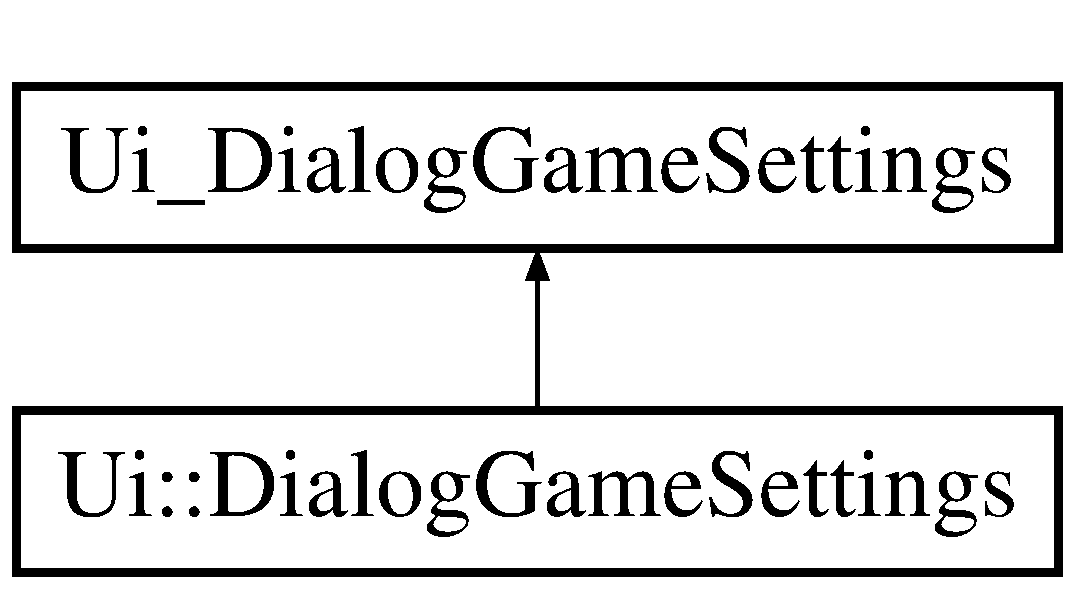
\includegraphics[height=2.000000cm]{class_ui_1_1_dialog_game_settings}
\end{center}
\end{figure}
\subsection*{Additional Inherited Members}


The documentation for this class was generated from the following file\-:\begin{DoxyCompactItemize}
\item 
Game/\hyperlink{ui__dialoggamesettings_8h}{ui\-\_\-dialoggamesettings.\-h}\end{DoxyCompactItemize}

\hypertarget{class_student_side_1_1_game_engine}{\section{Student\-Side\-:\-:Game\-Engine Class Reference}
\label{class_student_side_1_1_game_engine}\index{Student\-Side\-::\-Game\-Engine@{Student\-Side\-::\-Game\-Engine}}
}


The Init\-Game\-Engine class is for setting the game up. It launches dialog window for settings and initializes gamewindow.  




{\ttfamily \#include $<$gameengine.\-hh$>$}

Inheritance diagram for Student\-Side\-:\-:Game\-Engine\-:\begin{figure}[H]
\begin{center}
\leavevmode
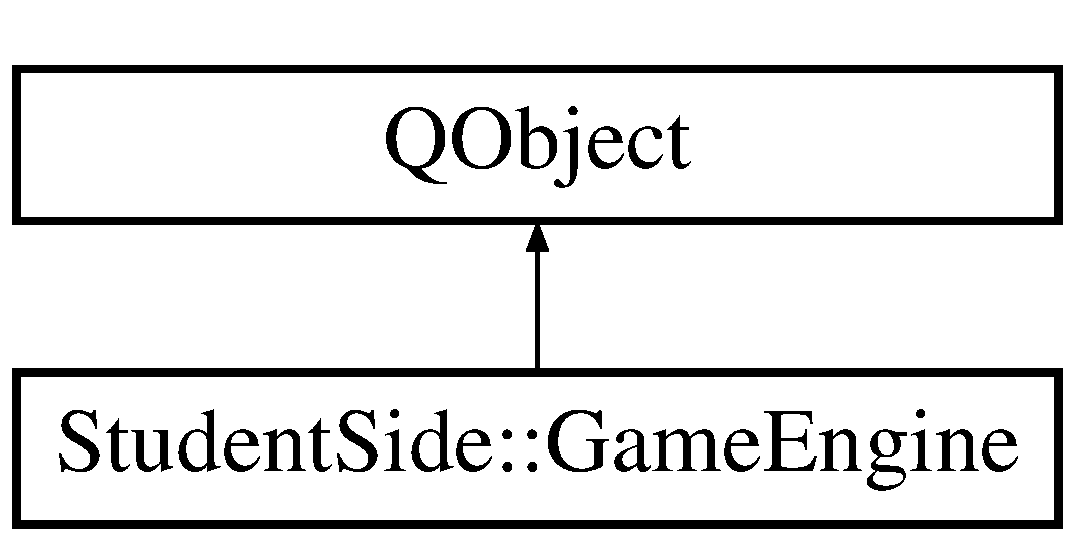
\includegraphics[height=2.000000cm]{class_student_side_1_1_game_engine}
\end{center}
\end{figure}
\subsection*{Public Member Functions}
\begin{DoxyCompactItemize}
\item 
\hyperlink{class_student_side_1_1_game_engine_a97ed7a110060bf799d7cc72f1444f160}{Game\-Engine} ()
\begin{DoxyCompactList}\small\item\em Constructor that initializes game settings and runs mainwindow. \end{DoxyCompactList}\end{DoxyCompactItemize}


\subsection{Detailed Description}
The Init\-Game\-Engine class is for setting the game up. It launches dialog window for settings and initializes gamewindow. 

\subsection{Constructor \& Destructor Documentation}
\hypertarget{class_student_side_1_1_game_engine_a97ed7a110060bf799d7cc72f1444f160}{\index{Student\-Side\-::\-Game\-Engine@{Student\-Side\-::\-Game\-Engine}!Game\-Engine@{Game\-Engine}}
\index{Game\-Engine@{Game\-Engine}!StudentSide::GameEngine@{Student\-Side\-::\-Game\-Engine}}
\subsubsection[{Game\-Engine}]{\setlength{\rightskip}{0pt plus 5cm}Student\-Side\-::\-Game\-Engine\-::\-Game\-Engine (
\begin{DoxyParamCaption}
{}
\end{DoxyParamCaption}
)}}\label{class_student_side_1_1_game_engine_a97ed7a110060bf799d7cc72f1444f160}


Constructor that initializes game settings and runs mainwindow. 



The documentation for this class was generated from the following files\-:\begin{DoxyCompactItemize}
\item 
\hyperlink{gameengine_8hh}{gameengine.\-hh}\item 
\hyperlink{gameengine_8cpp}{gameengine.\-cpp}\end{DoxyCompactItemize}

\hypertarget{class_ui_1_1_main_window}{\section{Ui\-:\-:Main\-Window Class Reference}
\label{class_ui_1_1_main_window}\index{Ui\-::\-Main\-Window@{Ui\-::\-Main\-Window}}
}


{\ttfamily \#include $<$ui\-\_\-mainwindow.\-h$>$}

Inheritance diagram for Ui\-:\-:Main\-Window\-:\begin{figure}[H]
\begin{center}
\leavevmode
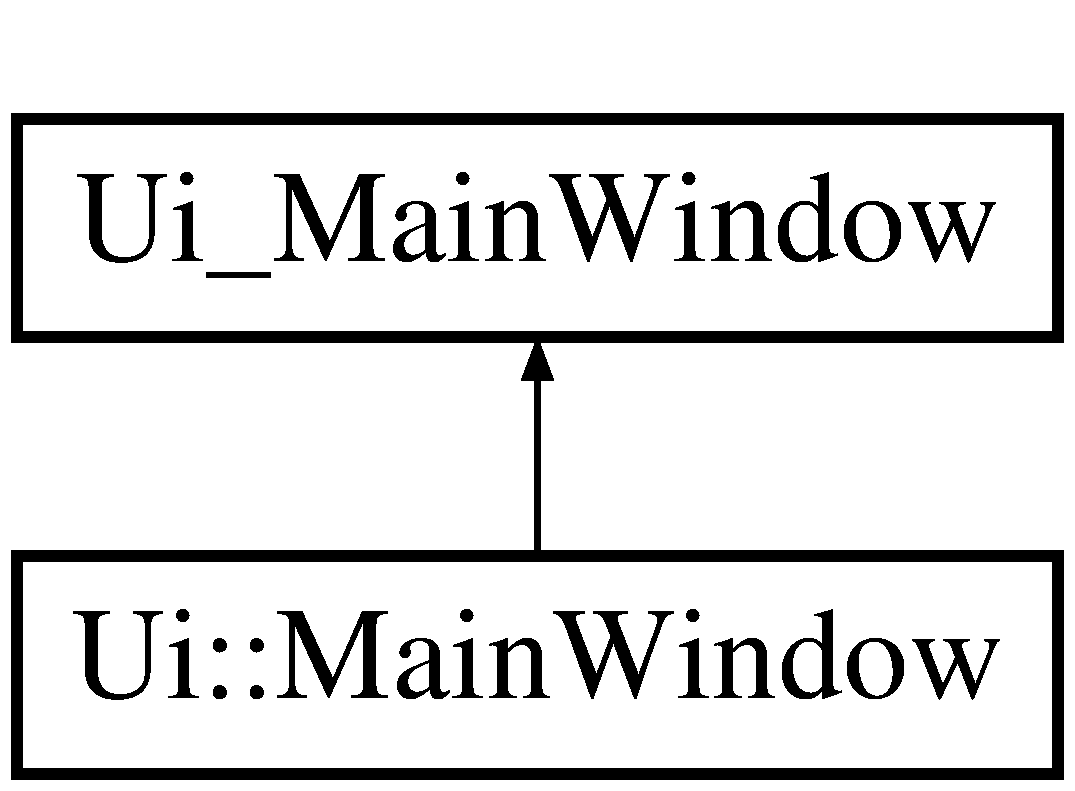
\includegraphics[height=2.000000cm]{class_ui_1_1_main_window}
\end{center}
\end{figure}
\subsection*{Additional Inherited Members}


The documentation for this class was generated from the following file\-:\begin{DoxyCompactItemize}
\item 
Game/\hyperlink{ui__mainwindow_8h}{ui\-\_\-mainwindow.\-h}\end{DoxyCompactItemize}

\hypertarget{class_student_side_1_1_mainwindow}{\section{Student\-Side\-:\-:Mainwindow Class Reference}
\label{class_student_side_1_1_mainwindow}\index{Student\-Side\-::\-Mainwindow@{Student\-Side\-::\-Mainwindow}}
}


The mainwindow class.  




{\ttfamily \#include $<$mainwindow.\-hh$>$}

Inheritance diagram for Student\-Side\-:\-:Mainwindow\-:\begin{figure}[H]
\begin{center}
\leavevmode
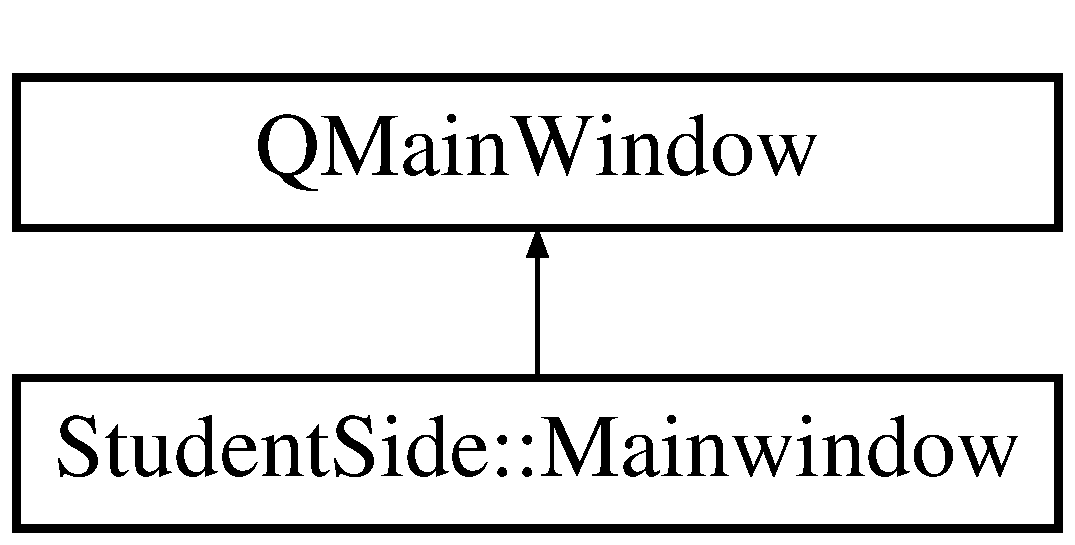
\includegraphics[height=2.000000cm]{class_student_side_1_1_mainwindow}
\end{center}
\end{figure}
\subsection*{Public Member Functions}
\begin{DoxyCompactItemize}
\item 
\hyperlink{class_student_side_1_1_mainwindow_a3be9249fcf6ae0439eab93841d84a4bc}{Mainwindow} (Q\-Widget $\ast$parent=nullptr)
\begin{DoxyCompactList}\small\item\em mainwindow constructor to create mainwindow userinterface. \end{DoxyCompactList}\item 
\hyperlink{class_student_side_1_1_mainwindow_abe12f13a949502ef80a5a4d8a649e410}{$\sim$\-Mainwindow} ()
\begin{DoxyCompactList}\small\item\em Destructor. \end{DoxyCompactList}\item 
void \hyperlink{class_student_side_1_1_mainwindow_a7cc5ee10d853012e479510ee80443d13}{set\-Background} (Q\-Pixmap \&image)
\begin{DoxyCompactList}\small\item\em set\-Background sets the game map to gamewindow \end{DoxyCompactList}\item 
void \hyperlink{class_student_side_1_1_mainwindow_aa6c19fef8cc6731de13b45764277ec67}{add\-Actor} (std\-::shared\-\_\-ptr$<$ Interface\-::\-I\-Actor $>$ actor)
\begin{DoxyCompactList}\small\item\em add\-Actor adds actor to mainwindow \end{DoxyCompactList}\item 
void \hyperlink{class_student_side_1_1_mainwindow_a27478d3419382f2bb8381c7c5af5c8ee}{add\-Stop} (std\-::shared\-\_\-ptr$<$ Interface\-::\-I\-Stop $>$ stop)
\begin{DoxyCompactList}\small\item\em add\-Stop adds bus stop to mainwindow \end{DoxyCompactList}\item 
void \hyperlink{class_student_side_1_1_mainwindow_a7c75210e41e3f9f962b77ebeaaa60811}{move\-Actor} (std\-::shared\-\_\-ptr$<$ Interface\-::\-I\-Actor $>$ actor, int \hyperlink{jquery_8js_a4c3eadaa5164016d2c340d495fc6e55e}{x}, int y)
\begin{DoxyCompactList}\small\item\em move\-Actor moves wanted actor in mainwindow \end{DoxyCompactList}\item 
void \hyperlink{class_student_side_1_1_mainwindow_ada6a000c4e9218c72425bad298e17ed9}{remove\-Actor} (std\-::shared\-\_\-ptr$<$ Interface\-::\-I\-Actor $>$ actor, bool points)
\begin{DoxyCompactList}\small\item\em remove\-Actor removes wanted actor from mainwindow \end{DoxyCompactList}\item 
void \hyperlink{class_student_side_1_1_mainwindow_ad97e4d9dd00a8d0b2b377f749504f98a}{add\-Player} (std\-::shared\-\_\-ptr$<$ \hyperlink{class_student_side_1_1_actor}{Student\-Side\-::\-Actor} $>$ player\-\_\-)
\begin{DoxyCompactList}\small\item\em add\-Player adds player to mainwindow \end{DoxyCompactList}\item 
Interface\-::\-Location \hyperlink{class_student_side_1_1_mainwindow_a487fd2b55286ec6c538c9bfbf8055dfb}{Give\-Player\-Location} ()
\begin{DoxyCompactList}\small\item\em Give\-Player\-Location gives player coordinates. \end{DoxyCompactList}\item 
\hyperlink{class_student_side_1_1player_actor}{Student\-Side\-::player\-Actor} $\ast$ \hyperlink{class_student_side_1_1_mainwindow_aa1eb590a67e0a49fd493c25ec20d189c}{return\-Player} ()
\begin{DoxyCompactList}\small\item\em return\-Player returns player graphics \end{DoxyCompactList}\item 
void \hyperlink{class_student_side_1_1_mainwindow_aed59f49514fa33ffdb6b77b0d0aa54f7}{add\-Points} ()
\begin{DoxyCompactList}\small\item\em add\-Points adds points to points\-\_\-lcd \end{DoxyCompactList}\item 
void \hyperlink{class_student_side_1_1_mainwindow_afa7eb3e3a86fab995d90d253015d3dc7}{take\-Stats} (std\-::shared\-\_\-ptr$<$ \hyperlink{class_student_side_1_1_statistics}{Student\-Side\-::\-Statistics} $>$ stats)
\begin{DoxyCompactList}\small\item\em take\-Stats \end{DoxyCompactList}\item 
Q\-Push\-Button $\ast$ \hyperlink{class_student_side_1_1_mainwindow_a0892eab493aace8eee0358c3d8e88d22}{get\-Start\-Button} ()
\begin{DoxyCompactList}\small\item\em get\-Start\-Button gives start\-Button \end{DoxyCompactList}\item 
Q\-Action $\ast$ \hyperlink{class_student_side_1_1_mainwindow_ae6bc2b06ca8ab22d7e5b5fbc10fbfe3b}{get\-Start\-Action} ()
\begin{DoxyCompactList}\small\item\em get\-Start\-Action return startaction to start the game from menubar \end{DoxyCompactList}\item 
void \hyperlink{class_student_side_1_1_mainwindow_acaa53f081e50381150eae32085f2aeea}{stop\-Game\-Timer} ()
\begin{DoxyCompactList}\small\item\em stop\-Game\-Timer stops game timer in lcd \end{DoxyCompactList}\item 
Q\-Label $\ast$ \hyperlink{class_student_side_1_1_mainwindow_a76f2312aed3a925d44111963a054512a}{get\-People\-Label} ()
\begin{DoxyCompactList}\small\item\em get\-People\-Label returns label containing people info \end{DoxyCompactList}\item 
bool \hyperlink{class_student_side_1_1_mainwindow_a413ff2fac6648addbd19f8a06a1305c7}{game\-Ended} ()
\begin{DoxyCompactList}\small\item\em game\-Ended return boolean if game is ended or not \end{DoxyCompactList}\item 
void \hyperlink{class_student_side_1_1_mainwindow_ace501f039bcececc0c7e891664bbaa50}{destroy\-Player} ()
\begin{DoxyCompactList}\small\item\em destroy\-Player destroys the player \end{DoxyCompactList}\item 
void \hyperlink{class_student_side_1_1_mainwindow_a66eadfc3c6e2f3e893b2142449b00f49}{add\-Nuke} (std\-::shared\-\_\-ptr$<$ \hyperlink{class_student_side_1_1_actor}{Student\-Side\-::\-Actor} $>$ nuke)
\begin{DoxyCompactList}\small\item\em add nuke to game \end{DoxyCompactList}\item 
bool \hyperlink{class_student_side_1_1_mainwindow_a9d393368717ac9f7cbaaae048b355e65}{is\-Nuked} ()
\begin{DoxyCompactList}\small\item\em get information if nuke has been launched by the player \end{DoxyCompactList}\end{DoxyCompactItemize}
\subsection*{Protected Member Functions}
\begin{DoxyCompactItemize}
\item 
void \hyperlink{class_student_side_1_1_mainwindow_a7dbeda19724837043388e76a17280284}{context\-Menu\-Event} (Q\-Context\-Menu\-Event $\ast$event) override
\end{DoxyCompactItemize}


\subsection{Detailed Description}
The mainwindow class. 

\subsection{Constructor \& Destructor Documentation}
\hypertarget{class_student_side_1_1_mainwindow_a3be9249fcf6ae0439eab93841d84a4bc}{\index{Student\-Side\-::\-Mainwindow@{Student\-Side\-::\-Mainwindow}!Mainwindow@{Mainwindow}}
\index{Mainwindow@{Mainwindow}!StudentSide::Mainwindow@{Student\-Side\-::\-Mainwindow}}
\subsubsection[{Mainwindow}]{\setlength{\rightskip}{0pt plus 5cm}Student\-Side\-::\-Mainwindow\-::\-Mainwindow (
\begin{DoxyParamCaption}
\item[{Q\-Widget $\ast$}]{parent = {\ttfamily nullptr}}
\end{DoxyParamCaption}
)\hspace{0.3cm}{\ttfamily [explicit]}}}\label{class_student_side_1_1_mainwindow_a3be9249fcf6ae0439eab93841d84a4bc}


mainwindow constructor to create mainwindow userinterface. 


\begin{DoxyParams}{Parameters}
{\em parent} & \\
\hline
\end{DoxyParams}
\begin{DoxyPrecond}{Precondition}
-\/ 
\end{DoxyPrecond}
\begin{DoxyPostcond}{Postcondition}
Exception guaranteed\-: nothrow 
\end{DoxyPostcond}
\hypertarget{class_student_side_1_1_mainwindow_abe12f13a949502ef80a5a4d8a649e410}{\index{Student\-Side\-::\-Mainwindow@{Student\-Side\-::\-Mainwindow}!$\sim$\-Mainwindow@{$\sim$\-Mainwindow}}
\index{$\sim$\-Mainwindow@{$\sim$\-Mainwindow}!StudentSide::Mainwindow@{Student\-Side\-::\-Mainwindow}}
\subsubsection[{$\sim$\-Mainwindow}]{\setlength{\rightskip}{0pt plus 5cm}Student\-Side\-::\-Mainwindow\-::$\sim$\-Mainwindow (
\begin{DoxyParamCaption}
{}
\end{DoxyParamCaption}
)}}\label{class_student_side_1_1_mainwindow_abe12f13a949502ef80a5a4d8a649e410}


Destructor. 



\subsection{Member Function Documentation}
\hypertarget{class_student_side_1_1_mainwindow_aa6c19fef8cc6731de13b45764277ec67}{\index{Student\-Side\-::\-Mainwindow@{Student\-Side\-::\-Mainwindow}!add\-Actor@{add\-Actor}}
\index{add\-Actor@{add\-Actor}!StudentSide::Mainwindow@{Student\-Side\-::\-Mainwindow}}
\subsubsection[{add\-Actor}]{\setlength{\rightskip}{0pt plus 5cm}void Student\-Side\-::\-Mainwindow\-::add\-Actor (
\begin{DoxyParamCaption}
\item[{std\-::shared\-\_\-ptr$<$ Interface\-::\-I\-Actor $>$}]{actor}
\end{DoxyParamCaption}
)}}\label{class_student_side_1_1_mainwindow_aa6c19fef8cc6731de13b45764277ec67}


add\-Actor adds actor to mainwindow 


\begin{DoxyParams}{Parameters}
{\em actor} & wanted actor to be added \\
\hline
\end{DoxyParams}
\begin{DoxyPrecond}{Precondition}
actor cant be null when addingt it 
\end{DoxyPrecond}
\begin{DoxyPostcond}{Postcondition}
Exception guaranteed\-: nothrow 
\end{DoxyPostcond}
\hypertarget{class_student_side_1_1_mainwindow_a66eadfc3c6e2f3e893b2142449b00f49}{\index{Student\-Side\-::\-Mainwindow@{Student\-Side\-::\-Mainwindow}!add\-Nuke@{add\-Nuke}}
\index{add\-Nuke@{add\-Nuke}!StudentSide::Mainwindow@{Student\-Side\-::\-Mainwindow}}
\subsubsection[{add\-Nuke}]{\setlength{\rightskip}{0pt plus 5cm}void Student\-Side\-::\-Mainwindow\-::add\-Nuke (
\begin{DoxyParamCaption}
\item[{std\-::shared\-\_\-ptr$<$ {\bf Student\-Side\-::\-Actor} $>$}]{nuke}
\end{DoxyParamCaption}
)}}\label{class_student_side_1_1_mainwindow_a66eadfc3c6e2f3e893b2142449b00f49}


add nuke to game 


\begin{DoxyParams}{Parameters}
{\em actor} & for nuke \\
\hline
\end{DoxyParams}
\begin{DoxyPrecond}{Precondition}
nuke must be found \-:D 
\end{DoxyPrecond}
\begin{DoxyPostcond}{Postcondition}
Exception guaranteed\-: nothrow 
\end{DoxyPostcond}
\hypertarget{class_student_side_1_1_mainwindow_ad97e4d9dd00a8d0b2b377f749504f98a}{\index{Student\-Side\-::\-Mainwindow@{Student\-Side\-::\-Mainwindow}!add\-Player@{add\-Player}}
\index{add\-Player@{add\-Player}!StudentSide::Mainwindow@{Student\-Side\-::\-Mainwindow}}
\subsubsection[{add\-Player}]{\setlength{\rightskip}{0pt plus 5cm}void Student\-Side\-::\-Mainwindow\-::add\-Player (
\begin{DoxyParamCaption}
\item[{std\-::shared\-\_\-ptr$<$ {\bf Student\-Side\-::\-Actor} $>$}]{player\-\_\-}
\end{DoxyParamCaption}
)}}\label{class_student_side_1_1_mainwindow_ad97e4d9dd00a8d0b2b377f749504f98a}


add\-Player adds player to mainwindow 


\begin{DoxyParams}{Parameters}
{\em player\-\_\-} & Player that user can move and play with \\
\hline
\end{DoxyParams}
\begin{DoxyPrecond}{Precondition}
player cant be null 
\end{DoxyPrecond}
\begin{DoxyPostcond}{Postcondition}
Exception guaranteed\-: minimum 
\end{DoxyPostcond}
\hypertarget{class_student_side_1_1_mainwindow_aed59f49514fa33ffdb6b77b0d0aa54f7}{\index{Student\-Side\-::\-Mainwindow@{Student\-Side\-::\-Mainwindow}!add\-Points@{add\-Points}}
\index{add\-Points@{add\-Points}!StudentSide::Mainwindow@{Student\-Side\-::\-Mainwindow}}
\subsubsection[{add\-Points}]{\setlength{\rightskip}{0pt plus 5cm}void Student\-Side\-::\-Mainwindow\-::add\-Points (
\begin{DoxyParamCaption}
{}
\end{DoxyParamCaption}
)}}\label{class_student_side_1_1_mainwindow_aed59f49514fa33ffdb6b77b0d0aa54f7}


add\-Points adds points to points\-\_\-lcd 

\begin{DoxyPrecond}{Precondition}
-\/ 
\end{DoxyPrecond}
\begin{DoxyPostcond}{Postcondition}
Exception guaranteed\-: nothrow 
\end{DoxyPostcond}
\hypertarget{class_student_side_1_1_mainwindow_a27478d3419382f2bb8381c7c5af5c8ee}{\index{Student\-Side\-::\-Mainwindow@{Student\-Side\-::\-Mainwindow}!add\-Stop@{add\-Stop}}
\index{add\-Stop@{add\-Stop}!StudentSide::Mainwindow@{Student\-Side\-::\-Mainwindow}}
\subsubsection[{add\-Stop}]{\setlength{\rightskip}{0pt plus 5cm}void Student\-Side\-::\-Mainwindow\-::add\-Stop (
\begin{DoxyParamCaption}
\item[{std\-::shared\-\_\-ptr$<$ Interface\-::\-I\-Stop $>$}]{stop}
\end{DoxyParamCaption}
)}}\label{class_student_side_1_1_mainwindow_a27478d3419382f2bb8381c7c5af5c8ee}


add\-Stop adds bus stop to mainwindow 


\begin{DoxyParams}{Parameters}
{\em stop} & Buss stop to be added \\
\hline
\end{DoxyParams}
\begin{DoxyPrecond}{Precondition}
stop must be found 
\end{DoxyPrecond}
\begin{DoxyPostcond}{Postcondition}
Exception guaranteed\-: nothrow 
\end{DoxyPostcond}
\hypertarget{class_student_side_1_1_mainwindow_a7dbeda19724837043388e76a17280284}{\index{Student\-Side\-::\-Mainwindow@{Student\-Side\-::\-Mainwindow}!context\-Menu\-Event@{context\-Menu\-Event}}
\index{context\-Menu\-Event@{context\-Menu\-Event}!StudentSide::Mainwindow@{Student\-Side\-::\-Mainwindow}}
\subsubsection[{context\-Menu\-Event}]{\setlength{\rightskip}{0pt plus 5cm}void Student\-Side\-::\-Mainwindow\-::context\-Menu\-Event (
\begin{DoxyParamCaption}
\item[{Q\-Context\-Menu\-Event $\ast$}]{event}
\end{DoxyParamCaption}
)\hspace{0.3cm}{\ttfamily [override]}, {\ttfamily [protected]}}}\label{class_student_side_1_1_mainwindow_a7dbeda19724837043388e76a17280284}
\hypertarget{class_student_side_1_1_mainwindow_ace501f039bcececc0c7e891664bbaa50}{\index{Student\-Side\-::\-Mainwindow@{Student\-Side\-::\-Mainwindow}!destroy\-Player@{destroy\-Player}}
\index{destroy\-Player@{destroy\-Player}!StudentSide::Mainwindow@{Student\-Side\-::\-Mainwindow}}
\subsubsection[{destroy\-Player}]{\setlength{\rightskip}{0pt plus 5cm}void Student\-Side\-::\-Mainwindow\-::destroy\-Player (
\begin{DoxyParamCaption}
{}
\end{DoxyParamCaption}
)}}\label{class_student_side_1_1_mainwindow_ace501f039bcececc0c7e891664bbaa50}


destroy\-Player destroys the player 

\begin{DoxyPrecond}{Precondition}
-\/ 
\end{DoxyPrecond}
\begin{DoxyPostcond}{Postcondition}
Exception guaranteed\-: nothrow 
\end{DoxyPostcond}
\hypertarget{class_student_side_1_1_mainwindow_a413ff2fac6648addbd19f8a06a1305c7}{\index{Student\-Side\-::\-Mainwindow@{Student\-Side\-::\-Mainwindow}!game\-Ended@{game\-Ended}}
\index{game\-Ended@{game\-Ended}!StudentSide::Mainwindow@{Student\-Side\-::\-Mainwindow}}
\subsubsection[{game\-Ended}]{\setlength{\rightskip}{0pt plus 5cm}bool Student\-Side\-::\-Mainwindow\-::game\-Ended (
\begin{DoxyParamCaption}
{}
\end{DoxyParamCaption}
)}}\label{class_student_side_1_1_mainwindow_a413ff2fac6648addbd19f8a06a1305c7}


game\-Ended return boolean if game is ended or not 

\begin{DoxyReturn}{Returns}
true when gane has ended, false otherwise 
\end{DoxyReturn}
\begin{DoxyPrecond}{Precondition}
-\/ 
\end{DoxyPrecond}
\begin{DoxyPostcond}{Postcondition}
Exception guaranteed\-: nothrow 
\end{DoxyPostcond}
\hypertarget{class_student_side_1_1_mainwindow_a76f2312aed3a925d44111963a054512a}{\index{Student\-Side\-::\-Mainwindow@{Student\-Side\-::\-Mainwindow}!get\-People\-Label@{get\-People\-Label}}
\index{get\-People\-Label@{get\-People\-Label}!StudentSide::Mainwindow@{Student\-Side\-::\-Mainwindow}}
\subsubsection[{get\-People\-Label}]{\setlength{\rightskip}{0pt plus 5cm}Q\-Label $\ast$ Student\-Side\-::\-Mainwindow\-::get\-People\-Label (
\begin{DoxyParamCaption}
{}
\end{DoxyParamCaption}
)}}\label{class_student_side_1_1_mainwindow_a76f2312aed3a925d44111963a054512a}


get\-People\-Label returns label containing people info 

\begin{DoxyReturn}{Returns}
Q\-Label 
\end{DoxyReturn}
\begin{DoxyPrecond}{Precondition}
-\/ 
\end{DoxyPrecond}
\begin{DoxyPostcond}{Postcondition}
Exception guaranteed\-: nothrow 
\end{DoxyPostcond}
\hypertarget{class_student_side_1_1_mainwindow_ae6bc2b06ca8ab22d7e5b5fbc10fbfe3b}{\index{Student\-Side\-::\-Mainwindow@{Student\-Side\-::\-Mainwindow}!get\-Start\-Action@{get\-Start\-Action}}
\index{get\-Start\-Action@{get\-Start\-Action}!StudentSide::Mainwindow@{Student\-Side\-::\-Mainwindow}}
\subsubsection[{get\-Start\-Action}]{\setlength{\rightskip}{0pt plus 5cm}Q\-Action $\ast$ Student\-Side\-::\-Mainwindow\-::get\-Start\-Action (
\begin{DoxyParamCaption}
{}
\end{DoxyParamCaption}
)}}\label{class_student_side_1_1_mainwindow_ae6bc2b06ca8ab22d7e5b5fbc10fbfe3b}


get\-Start\-Action return startaction to start the game from menubar 

\begin{DoxyReturn}{Returns}
star\-Action 
\end{DoxyReturn}
\begin{DoxyPrecond}{Precondition}
-\/ 
\end{DoxyPrecond}
\begin{DoxyPostcond}{Postcondition}
Exception guaranteed\-: nothrow 
\end{DoxyPostcond}
\hypertarget{class_student_side_1_1_mainwindow_a0892eab493aace8eee0358c3d8e88d22}{\index{Student\-Side\-::\-Mainwindow@{Student\-Side\-::\-Mainwindow}!get\-Start\-Button@{get\-Start\-Button}}
\index{get\-Start\-Button@{get\-Start\-Button}!StudentSide::Mainwindow@{Student\-Side\-::\-Mainwindow}}
\subsubsection[{get\-Start\-Button}]{\setlength{\rightskip}{0pt plus 5cm}Q\-Push\-Button $\ast$ Student\-Side\-::\-Mainwindow\-::get\-Start\-Button (
\begin{DoxyParamCaption}
{}
\end{DoxyParamCaption}
)}}\label{class_student_side_1_1_mainwindow_a0892eab493aace8eee0358c3d8e88d22}


get\-Start\-Button gives start\-Button 

\begin{DoxyReturn}{Returns}
star\-Button of userinterface 
\end{DoxyReturn}
\begin{DoxyPrecond}{Precondition}
-\/ 
\end{DoxyPrecond}
\begin{DoxyPostcond}{Postcondition}
Exception guaranteed\-: nothrow 
\end{DoxyPostcond}
\hypertarget{class_student_side_1_1_mainwindow_a487fd2b55286ec6c538c9bfbf8055dfb}{\index{Student\-Side\-::\-Mainwindow@{Student\-Side\-::\-Mainwindow}!Give\-Player\-Location@{Give\-Player\-Location}}
\index{Give\-Player\-Location@{Give\-Player\-Location}!StudentSide::Mainwindow@{Student\-Side\-::\-Mainwindow}}
\subsubsection[{Give\-Player\-Location}]{\setlength{\rightskip}{0pt plus 5cm}Interface\-::\-Location Student\-Side\-::\-Mainwindow\-::\-Give\-Player\-Location (
\begin{DoxyParamCaption}
{}
\end{DoxyParamCaption}
)}}\label{class_student_side_1_1_mainwindow_a487fd2b55286ec6c538c9bfbf8055dfb}


Give\-Player\-Location gives player coordinates. 

\begin{DoxyReturn}{Returns}
location of player 
\end{DoxyReturn}
\hypertarget{class_student_side_1_1_mainwindow_a9d393368717ac9f7cbaaae048b355e65}{\index{Student\-Side\-::\-Mainwindow@{Student\-Side\-::\-Mainwindow}!is\-Nuked@{is\-Nuked}}
\index{is\-Nuked@{is\-Nuked}!StudentSide::Mainwindow@{Student\-Side\-::\-Mainwindow}}
\subsubsection[{is\-Nuked}]{\setlength{\rightskip}{0pt plus 5cm}bool Student\-Side\-::\-Mainwindow\-::is\-Nuked (
\begin{DoxyParamCaption}
{}
\end{DoxyParamCaption}
)}}\label{class_student_side_1_1_mainwindow_a9d393368717ac9f7cbaaae048b355e65}


get information if nuke has been launched by the player 

\begin{DoxyPrecond}{Precondition}
-\/ 
\end{DoxyPrecond}
\begin{DoxyPostcond}{Postcondition}
Exception guaranteed\-: minimum 
\end{DoxyPostcond}
\hypertarget{class_student_side_1_1_mainwindow_a7c75210e41e3f9f962b77ebeaaa60811}{\index{Student\-Side\-::\-Mainwindow@{Student\-Side\-::\-Mainwindow}!move\-Actor@{move\-Actor}}
\index{move\-Actor@{move\-Actor}!StudentSide::Mainwindow@{Student\-Side\-::\-Mainwindow}}
\subsubsection[{move\-Actor}]{\setlength{\rightskip}{0pt plus 5cm}void Student\-Side\-::\-Mainwindow\-::move\-Actor (
\begin{DoxyParamCaption}
\item[{std\-::shared\-\_\-ptr$<$ Interface\-::\-I\-Actor $>$}]{actor, }
\item[{int}]{x, }
\item[{int}]{y}
\end{DoxyParamCaption}
)}}\label{class_student_side_1_1_mainwindow_a7c75210e41e3f9f962b77ebeaaa60811}


move\-Actor moves wanted actor in mainwindow 


\begin{DoxyParams}{Parameters}
{\em actor} & \hyperlink{class_student_side_1_1_actor}{Actor} to be moved \\
\hline
{\em x} & x-\/coordinate \\
\hline
{\em y} & y-\/coordinate \\
\hline
\end{DoxyParams}
\begin{DoxyPrecond}{Precondition}
actor must be found and x and y coordinates do not pass map borders 
\end{DoxyPrecond}
\begin{DoxyPostcond}{Postcondition}
Exception guaranteed\-: minimum 
\end{DoxyPostcond}
\hypertarget{class_student_side_1_1_mainwindow_ada6a000c4e9218c72425bad298e17ed9}{\index{Student\-Side\-::\-Mainwindow@{Student\-Side\-::\-Mainwindow}!remove\-Actor@{remove\-Actor}}
\index{remove\-Actor@{remove\-Actor}!StudentSide::Mainwindow@{Student\-Side\-::\-Mainwindow}}
\subsubsection[{remove\-Actor}]{\setlength{\rightskip}{0pt plus 5cm}void Student\-Side\-::\-Mainwindow\-::remove\-Actor (
\begin{DoxyParamCaption}
\item[{std\-::shared\-\_\-ptr$<$ Interface\-::\-I\-Actor $>$}]{actor, }
\item[{bool}]{points}
\end{DoxyParamCaption}
)}}\label{class_student_side_1_1_mainwindow_ada6a000c4e9218c72425bad298e17ed9}


remove\-Actor removes wanted actor from mainwindow 


\begin{DoxyParams}{Parameters}
{\em actor} & \hyperlink{class_student_side_1_1_actor}{Actor} to be removed \\
\hline
\end{DoxyParams}
\begin{DoxyPrecond}{Precondition}
actor must be found 
\end{DoxyPrecond}
\begin{DoxyPostcond}{Postcondition}
Exception guaranteed\-: nothrow 
\end{DoxyPostcond}
\hypertarget{class_student_side_1_1_mainwindow_aa1eb590a67e0a49fd493c25ec20d189c}{\index{Student\-Side\-::\-Mainwindow@{Student\-Side\-::\-Mainwindow}!return\-Player@{return\-Player}}
\index{return\-Player@{return\-Player}!StudentSide::Mainwindow@{Student\-Side\-::\-Mainwindow}}
\subsubsection[{return\-Player}]{\setlength{\rightskip}{0pt plus 5cm}{\bf player\-Actor} $\ast$ Student\-Side\-::\-Mainwindow\-::return\-Player (
\begin{DoxyParamCaption}
{}
\end{DoxyParamCaption}
)}}\label{class_student_side_1_1_mainwindow_aa1eb590a67e0a49fd493c25ec20d189c}


return\-Player returns player graphics 

\begin{DoxyReturn}{Returns}
graphics of player 
\end{DoxyReturn}
\begin{DoxyPrecond}{Precondition}
-\/ 
\end{DoxyPrecond}
\begin{DoxyPostcond}{Postcondition}
Exception guaranteed\-: minimum 
\end{DoxyPostcond}
\hypertarget{class_student_side_1_1_mainwindow_a7cc5ee10d853012e479510ee80443d13}{\index{Student\-Side\-::\-Mainwindow@{Student\-Side\-::\-Mainwindow}!set\-Background@{set\-Background}}
\index{set\-Background@{set\-Background}!StudentSide::Mainwindow@{Student\-Side\-::\-Mainwindow}}
\subsubsection[{set\-Background}]{\setlength{\rightskip}{0pt plus 5cm}void Student\-Side\-::\-Mainwindow\-::set\-Background (
\begin{DoxyParamCaption}
\item[{Q\-Pixmap \&}]{image}
\end{DoxyParamCaption}
)}}\label{class_student_side_1_1_mainwindow_a7cc5ee10d853012e479510ee80443d13}


set\-Background sets the game map to gamewindow 


\begin{DoxyParams}{Parameters}
{\em image} & Map image \\
\hline
\end{DoxyParams}
\begin{DoxyPrecond}{Precondition}
-\/ 
\end{DoxyPrecond}
\begin{DoxyPostcond}{Postcondition}
Exception guaranteed\-: nothrow 
\end{DoxyPostcond}
\hypertarget{class_student_side_1_1_mainwindow_acaa53f081e50381150eae32085f2aeea}{\index{Student\-Side\-::\-Mainwindow@{Student\-Side\-::\-Mainwindow}!stop\-Game\-Timer@{stop\-Game\-Timer}}
\index{stop\-Game\-Timer@{stop\-Game\-Timer}!StudentSide::Mainwindow@{Student\-Side\-::\-Mainwindow}}
\subsubsection[{stop\-Game\-Timer}]{\setlength{\rightskip}{0pt plus 5cm}void Student\-Side\-::\-Mainwindow\-::stop\-Game\-Timer (
\begin{DoxyParamCaption}
{}
\end{DoxyParamCaption}
)}}\label{class_student_side_1_1_mainwindow_acaa53f081e50381150eae32085f2aeea}


stop\-Game\-Timer stops game timer in lcd 

\begin{DoxyPrecond}{Precondition}
-\/ 
\end{DoxyPrecond}
\begin{DoxyPostcond}{Postcondition}
Exception guaranteed\-: nothrow 
\end{DoxyPostcond}
\hypertarget{class_student_side_1_1_mainwindow_afa7eb3e3a86fab995d90d253015d3dc7}{\index{Student\-Side\-::\-Mainwindow@{Student\-Side\-::\-Mainwindow}!take\-Stats@{take\-Stats}}
\index{take\-Stats@{take\-Stats}!StudentSide::Mainwindow@{Student\-Side\-::\-Mainwindow}}
\subsubsection[{take\-Stats}]{\setlength{\rightskip}{0pt plus 5cm}void Student\-Side\-::\-Mainwindow\-::take\-Stats (
\begin{DoxyParamCaption}
\item[{std\-::shared\-\_\-ptr$<$ {\bf Student\-Side\-::\-Statistics} $>$}]{stats}
\end{DoxyParamCaption}
)}}\label{class_student_side_1_1_mainwindow_afa7eb3e3a86fab995d90d253015d3dc7}


take\-Stats 


\begin{DoxyParams}{Parameters}
{\em stats} & \\
\hline
\end{DoxyParams}
\begin{DoxyPrecond}{Precondition}
stats must be found 
\end{DoxyPrecond}
\begin{DoxyPostcond}{Postcondition}
Exception guaranteed\-: nothrow 
\end{DoxyPostcond}


The documentation for this class was generated from the following files\-:\begin{DoxyCompactItemize}
\item 
Game/\hyperlink{mainwindow_8hh}{mainwindow.\-hh}\item 
Game/\hyperlink{mainwindow_8cpp}{mainwindow.\-cpp}\end{DoxyCompactItemize}

\hypertarget{class_student_side_1_1_nuke_actor}{\section{Student\-Side\-:\-:Nuke\-Actor Class Reference}
\label{class_student_side_1_1_nuke_actor}\index{Student\-Side\-::\-Nuke\-Actor@{Student\-Side\-::\-Nuke\-Actor}}
}


The \hyperlink{class_student_side_1_1_nuke_actor}{Nuke\-Actor} class.  




{\ttfamily \#include $<$nukeactor.\-hh$>$}

Inheritance diagram for Student\-Side\-:\-:Nuke\-Actor\-:\begin{figure}[H]
\begin{center}
\leavevmode
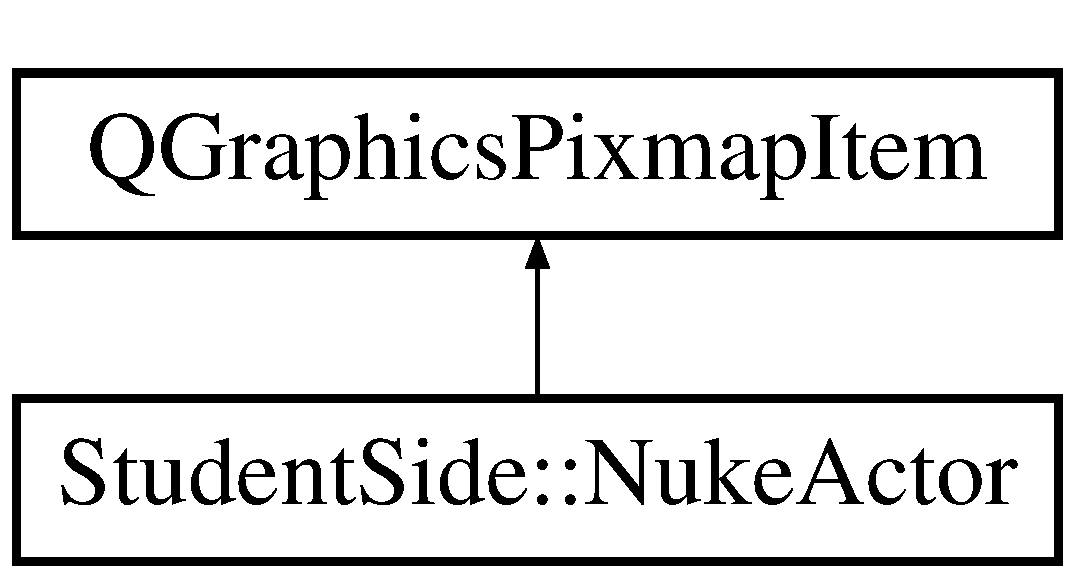
\includegraphics[height=2.000000cm]{class_student_side_1_1_nuke_actor}
\end{center}
\end{figure}
\subsection*{Public Member Functions}
\begin{DoxyCompactItemize}
\item 
\hyperlink{class_student_side_1_1_nuke_actor_abc65d6502333d97c4cd1beb37bdaa163}{Nuke\-Actor} (Interface\-::\-Location location)
\begin{DoxyCompactList}\small\item\em \hyperlink{class_student_side_1_1_nuke_actor}{Nuke\-Actor} gets nukeactor to the map. \end{DoxyCompactList}\item 
\hyperlink{class_student_side_1_1_nuke_actor_a1198514f0e17e36e243b344331c543ac}{$\sim$\-Nuke\-Actor} ()
\begin{DoxyCompactList}\small\item\em Destructor. \end{DoxyCompactList}\end{DoxyCompactItemize}


\subsection{Detailed Description}
The \hyperlink{class_student_side_1_1_nuke_actor}{Nuke\-Actor} class. 

\subsection{Constructor \& Destructor Documentation}
\hypertarget{class_student_side_1_1_nuke_actor_abc65d6502333d97c4cd1beb37bdaa163}{\index{Student\-Side\-::\-Nuke\-Actor@{Student\-Side\-::\-Nuke\-Actor}!Nuke\-Actor@{Nuke\-Actor}}
\index{Nuke\-Actor@{Nuke\-Actor}!StudentSide::NukeActor@{Student\-Side\-::\-Nuke\-Actor}}
\subsubsection[{Nuke\-Actor}]{\setlength{\rightskip}{0pt plus 5cm}Student\-Side\-::\-Nuke\-Actor\-::\-Nuke\-Actor (
\begin{DoxyParamCaption}
\item[{Interface\-::\-Location}]{location}
\end{DoxyParamCaption}
)}}\label{class_student_side_1_1_nuke_actor_abc65d6502333d97c4cd1beb37bdaa163}


\hyperlink{class_student_side_1_1_nuke_actor}{Nuke\-Actor} gets nukeactor to the map. 


\begin{DoxyParams}{Parameters}
{\em location} & Location to draw the nuke actor \\
\hline
\end{DoxyParams}
\begin{DoxyPrecond}{Precondition}
Location must be inside map coordinates 
\end{DoxyPrecond}
\begin{DoxyPostcond}{Postcondition}
Exception guaranteed\-: nothrow 
\end{DoxyPostcond}
\hypertarget{class_student_side_1_1_nuke_actor_a1198514f0e17e36e243b344331c543ac}{\index{Student\-Side\-::\-Nuke\-Actor@{Student\-Side\-::\-Nuke\-Actor}!$\sim$\-Nuke\-Actor@{$\sim$\-Nuke\-Actor}}
\index{$\sim$\-Nuke\-Actor@{$\sim$\-Nuke\-Actor}!StudentSide::NukeActor@{Student\-Side\-::\-Nuke\-Actor}}
\subsubsection[{$\sim$\-Nuke\-Actor}]{\setlength{\rightskip}{0pt plus 5cm}Student\-Side\-::\-Nuke\-Actor\-::$\sim$\-Nuke\-Actor (
\begin{DoxyParamCaption}
{}
\end{DoxyParamCaption}
)}}\label{class_student_side_1_1_nuke_actor_a1198514f0e17e36e243b344331c543ac}


Destructor. 



The documentation for this class was generated from the following files\-:\begin{DoxyCompactItemize}
\item 
Game/\hyperlink{nukeactor_8hh}{nukeactor.\-hh}\item 
Game/\hyperlink{nukeactor_8cpp}{nukeactor.\-cpp}\end{DoxyCompactItemize}

\hypertarget{class_student_side_1_1player_actor}{\section{Student\-Side\-:\-:player\-Actor Class Reference}
\label{class_student_side_1_1player_actor}\index{Student\-Side\-::player\-Actor@{Student\-Side\-::player\-Actor}}
}


{\ttfamily \#include $<$playeractor.\-hh$>$}

Inheritance diagram for Student\-Side\-:\-:player\-Actor\-:\begin{figure}[H]
\begin{center}
\leavevmode
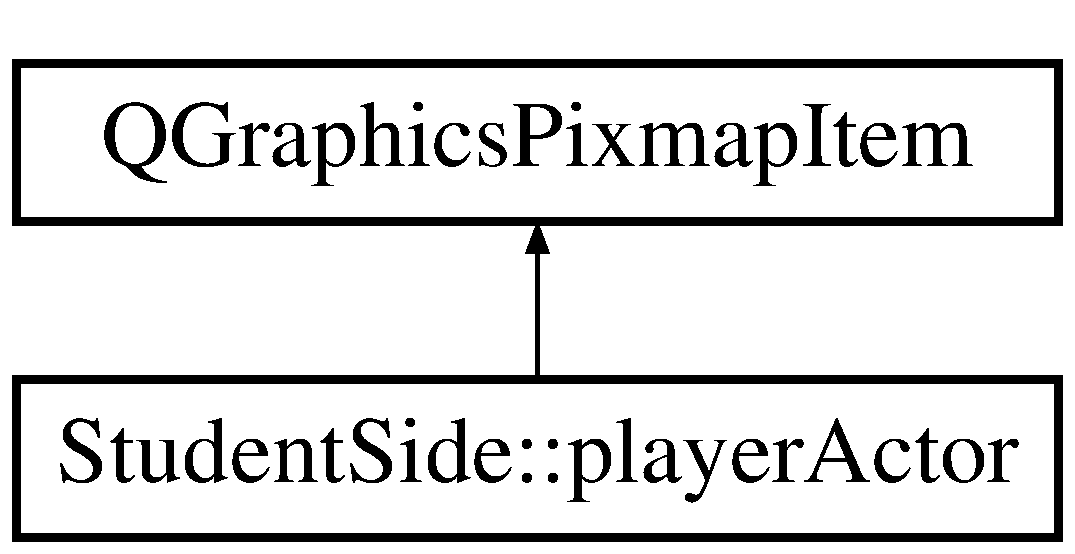
\includegraphics[height=2.000000cm]{class_student_side_1_1player_actor}
\end{center}
\end{figure}
\subsection*{Public Member Functions}
\begin{DoxyCompactItemize}
\item 
\hyperlink{class_student_side_1_1player_actor_a58a39690b97b3442cd7e01a3fae5b8bb}{player\-Actor} (Interface\-::\-Location location)
\begin{DoxyCompactList}\small\item\em \hyperlink{class_student_side_1_1player_actor}{player\-Actor} constructor to set player to map \end{DoxyCompactList}\item 
void \hyperlink{class_student_side_1_1player_actor_a6f2221903208ea8475f4c27efa76e842}{change\-Position} (int \hyperlink{jquery_8js_a4c3eadaa5164016d2c340d495fc6e55e}{x}, int y)
\begin{DoxyCompactList}\small\item\em change\-Position changes players position \end{DoxyCompactList}\item 
void \hyperlink{class_student_side_1_1player_actor_a9feca7b2dd13c5a8febc7c54aac8940e}{key\-Press\-Event} (Q\-Key\-Event $\ast$event) override
\begin{DoxyCompactList}\small\item\em key\-Press\-Event reads keyinputs \end{DoxyCompactList}\item 
Interface\-::\-Location \hyperlink{class_student_side_1_1player_actor_a551fd8c11c43a9ebb0401ed0ee9ef63c}{give\-Location} ()
\begin{DoxyCompactList}\small\item\em give\-Location returns location of player \end{DoxyCompactList}\item 
void \hyperlink{class_student_side_1_1player_actor_a2d1a691ca176eb1436febd320d2040ab}{add\-Nuke} ()
\begin{DoxyCompactList}\small\item\em Marks the nuke to be usable the player. \end{DoxyCompactList}\item 
bool \hyperlink{class_student_side_1_1player_actor_a54888fe10ceb2fdcd7b99e7f5c227da9}{is\-Nuked} ()
\begin{DoxyCompactList}\small\item\em tells if the nuke is used by the player \end{DoxyCompactList}\end{DoxyCompactItemize}


\subsection{Constructor \& Destructor Documentation}
\hypertarget{class_student_side_1_1player_actor_a58a39690b97b3442cd7e01a3fae5b8bb}{\index{Student\-Side\-::player\-Actor@{Student\-Side\-::player\-Actor}!player\-Actor@{player\-Actor}}
\index{player\-Actor@{player\-Actor}!StudentSide::playerActor@{Student\-Side\-::player\-Actor}}
\subsubsection[{player\-Actor}]{\setlength{\rightskip}{0pt plus 5cm}Student\-Side\-::player\-Actor\-::player\-Actor (
\begin{DoxyParamCaption}
\item[{Interface\-::\-Location}]{location}
\end{DoxyParamCaption}
)}}\label{class_student_side_1_1player_actor_a58a39690b97b3442cd7e01a3fae5b8bb}


\hyperlink{class_student_side_1_1player_actor}{player\-Actor} constructor to set player to map 


\begin{DoxyParams}{Parameters}
{\em location} & Location to set player \\
\hline
\end{DoxyParams}
\begin{DoxyPrecond}{Precondition}
Location must be inside map coordinates 
\end{DoxyPrecond}


\subsection{Member Function Documentation}
\hypertarget{class_student_side_1_1player_actor_a2d1a691ca176eb1436febd320d2040ab}{\index{Student\-Side\-::player\-Actor@{Student\-Side\-::player\-Actor}!add\-Nuke@{add\-Nuke}}
\index{add\-Nuke@{add\-Nuke}!StudentSide::playerActor@{Student\-Side\-::player\-Actor}}
\subsubsection[{add\-Nuke}]{\setlength{\rightskip}{0pt plus 5cm}void Student\-Side\-::player\-Actor\-::add\-Nuke (
\begin{DoxyParamCaption}
{}
\end{DoxyParamCaption}
)}}\label{class_student_side_1_1player_actor_a2d1a691ca176eb1436febd320d2040ab}


Marks the nuke to be usable the player. 

\hypertarget{class_student_side_1_1player_actor_a6f2221903208ea8475f4c27efa76e842}{\index{Student\-Side\-::player\-Actor@{Student\-Side\-::player\-Actor}!change\-Position@{change\-Position}}
\index{change\-Position@{change\-Position}!StudentSide::playerActor@{Student\-Side\-::player\-Actor}}
\subsubsection[{change\-Position}]{\setlength{\rightskip}{0pt plus 5cm}void Student\-Side\-::player\-Actor\-::change\-Position (
\begin{DoxyParamCaption}
\item[{int}]{x, }
\item[{int}]{y}
\end{DoxyParamCaption}
)}}\label{class_student_side_1_1player_actor_a6f2221903208ea8475f4c27efa76e842}


change\-Position changes players position 


\begin{DoxyParams}{Parameters}
{\em x} & x-\/coordinate \\
\hline
{\em y} & y-\/coordinate \\
\hline
\end{DoxyParams}
\begin{DoxyPrecond}{Precondition}
Coordinates must be inside map coordinates 
\end{DoxyPrecond}
\hypertarget{class_student_side_1_1player_actor_a551fd8c11c43a9ebb0401ed0ee9ef63c}{\index{Student\-Side\-::player\-Actor@{Student\-Side\-::player\-Actor}!give\-Location@{give\-Location}}
\index{give\-Location@{give\-Location}!StudentSide::playerActor@{Student\-Side\-::player\-Actor}}
\subsubsection[{give\-Location}]{\setlength{\rightskip}{0pt plus 5cm}Interface\-::\-Location Student\-Side\-::player\-Actor\-::give\-Location (
\begin{DoxyParamCaption}
{}
\end{DoxyParamCaption}
)}}\label{class_student_side_1_1player_actor_a551fd8c11c43a9ebb0401ed0ee9ef63c}


give\-Location returns location of player 

\begin{DoxyReturn}{Returns}
location of player 
\end{DoxyReturn}
\hypertarget{class_student_side_1_1player_actor_a54888fe10ceb2fdcd7b99e7f5c227da9}{\index{Student\-Side\-::player\-Actor@{Student\-Side\-::player\-Actor}!is\-Nuked@{is\-Nuked}}
\index{is\-Nuked@{is\-Nuked}!StudentSide::playerActor@{Student\-Side\-::player\-Actor}}
\subsubsection[{is\-Nuked}]{\setlength{\rightskip}{0pt plus 5cm}bool Student\-Side\-::player\-Actor\-::is\-Nuked (
\begin{DoxyParamCaption}
{}
\end{DoxyParamCaption}
)}}\label{class_student_side_1_1player_actor_a54888fe10ceb2fdcd7b99e7f5c227da9}


tells if the nuke is used by the player 

\begin{DoxyReturn}{Returns}
the boolean value of the status of the nuke 
\end{DoxyReturn}
\hypertarget{class_student_side_1_1player_actor_a9feca7b2dd13c5a8febc7c54aac8940e}{\index{Student\-Side\-::player\-Actor@{Student\-Side\-::player\-Actor}!key\-Press\-Event@{key\-Press\-Event}}
\index{key\-Press\-Event@{key\-Press\-Event}!StudentSide::playerActor@{Student\-Side\-::player\-Actor}}
\subsubsection[{key\-Press\-Event}]{\setlength{\rightskip}{0pt plus 5cm}void Student\-Side\-::player\-Actor\-::key\-Press\-Event (
\begin{DoxyParamCaption}
\item[{Q\-Key\-Event $\ast$}]{event}
\end{DoxyParamCaption}
)\hspace{0.3cm}{\ttfamily [override]}}}\label{class_student_side_1_1player_actor_a9feca7b2dd13c5a8febc7c54aac8940e}


key\-Press\-Event reads keyinputs 


\begin{DoxyParams}{Parameters}
{\em event} & from key presses \\
\hline
\end{DoxyParams}


The documentation for this class was generated from the following files\-:\begin{DoxyCompactItemize}
\item 
Game/\hyperlink{playeractor_8hh}{playeractor.\-hh}\item 
Game/\hyperlink{playeractor_8cpp}{playeractor.\-cpp}\end{DoxyCompactItemize}

\hypertarget{structqt__meta__stringdata___student_side_____dialog_game_settings__t}{\section{qt\-\_\-meta\-\_\-stringdata\-\_\-\-Student\-Side\-\_\-\-\_\-\-Dialog\-Game\-Settings\-\_\-t Struct Reference}
\label{structqt__meta__stringdata___student_side_____dialog_game_settings__t}\index{qt\-\_\-meta\-\_\-stringdata\-\_\-\-Student\-Side\-\_\-\-\_\-\-Dialog\-Game\-Settings\-\_\-t@{qt\-\_\-meta\-\_\-stringdata\-\_\-\-Student\-Side\-\_\-\-\_\-\-Dialog\-Game\-Settings\-\_\-t}}
}
\subsection*{Public Attributes}
\begin{DoxyCompactItemize}
\item 
Q\-Byte\-Array\-Data \hyperlink{structqt__meta__stringdata___student_side_____dialog_game_settings__t_a7ff98fd212e598560d745b5514d4404a}{data} \mbox{[}10\mbox{]}
\item 
char \hyperlink{structqt__meta__stringdata___student_side_____dialog_game_settings__t_a003ddd07e53c401c4007209b65ea5da5}{stringdata0} \mbox{[}122\mbox{]}
\end{DoxyCompactItemize}


\subsection{Member Data Documentation}
\hypertarget{structqt__meta__stringdata___student_side_____dialog_game_settings__t_a7ff98fd212e598560d745b5514d4404a}{\index{qt\-\_\-meta\-\_\-stringdata\-\_\-\-Student\-Side\-\_\-\-\_\-\-Dialog\-Game\-Settings\-\_\-t@{qt\-\_\-meta\-\_\-stringdata\-\_\-\-Student\-Side\-\_\-\-\_\-\-Dialog\-Game\-Settings\-\_\-t}!data@{data}}
\index{data@{data}!qt_meta_stringdata_StudentSide__DialogGameSettings_t@{qt\-\_\-meta\-\_\-stringdata\-\_\-\-Student\-Side\-\_\-\-\_\-\-Dialog\-Game\-Settings\-\_\-t}}
\subsubsection[{data}]{\setlength{\rightskip}{0pt plus 5cm}Q\-Byte\-Array\-Data qt\-\_\-meta\-\_\-stringdata\-\_\-\-Student\-Side\-\_\-\-\_\-\-Dialog\-Game\-Settings\-\_\-t\-::data\mbox{[}10\mbox{]}}}\label{structqt__meta__stringdata___student_side_____dialog_game_settings__t_a7ff98fd212e598560d745b5514d4404a}
\hypertarget{structqt__meta__stringdata___student_side_____dialog_game_settings__t_a003ddd07e53c401c4007209b65ea5da5}{\index{qt\-\_\-meta\-\_\-stringdata\-\_\-\-Student\-Side\-\_\-\-\_\-\-Dialog\-Game\-Settings\-\_\-t@{qt\-\_\-meta\-\_\-stringdata\-\_\-\-Student\-Side\-\_\-\-\_\-\-Dialog\-Game\-Settings\-\_\-t}!stringdata0@{stringdata0}}
\index{stringdata0@{stringdata0}!qt_meta_stringdata_StudentSide__DialogGameSettings_t@{qt\-\_\-meta\-\_\-stringdata\-\_\-\-Student\-Side\-\_\-\-\_\-\-Dialog\-Game\-Settings\-\_\-t}}
\subsubsection[{stringdata0}]{\setlength{\rightskip}{0pt plus 5cm}char qt\-\_\-meta\-\_\-stringdata\-\_\-\-Student\-Side\-\_\-\-\_\-\-Dialog\-Game\-Settings\-\_\-t\-::stringdata0\mbox{[}122\mbox{]}}}\label{structqt__meta__stringdata___student_side_____dialog_game_settings__t_a003ddd07e53c401c4007209b65ea5da5}


The documentation for this struct was generated from the following file\-:\begin{DoxyCompactItemize}
\item 
Game/\hyperlink{moc__dialoggamesettings_8cpp}{moc\-\_\-dialoggamesettings.\-cpp}\end{DoxyCompactItemize}

\hypertarget{structqt__meta__stringdata___student_side_____game_engine__t}{\section{qt\-\_\-meta\-\_\-stringdata\-\_\-\-Student\-Side\-\_\-\-\_\-\-Game\-Engine\-\_\-t Struct Reference}
\label{structqt__meta__stringdata___student_side_____game_engine__t}\index{qt\-\_\-meta\-\_\-stringdata\-\_\-\-Student\-Side\-\_\-\-\_\-\-Game\-Engine\-\_\-t@{qt\-\_\-meta\-\_\-stringdata\-\_\-\-Student\-Side\-\_\-\-\_\-\-Game\-Engine\-\_\-t}}
}
\subsection*{Public Attributes}
\begin{DoxyCompactItemize}
\item 
Q\-Byte\-Array\-Data \hyperlink{structqt__meta__stringdata___student_side_____game_engine__t_aa6366f6e71cef2c92fa62156715535e6}{data} \mbox{[}5\mbox{]}
\item 
char \hyperlink{structqt__meta__stringdata___student_side_____game_engine__t_ab37bb3a2060f5e5cdfb8c0b067c220db}{stringdata0} \mbox{[}56\mbox{]}
\end{DoxyCompactItemize}


\subsection{Member Data Documentation}
\hypertarget{structqt__meta__stringdata___student_side_____game_engine__t_aa6366f6e71cef2c92fa62156715535e6}{\index{qt\-\_\-meta\-\_\-stringdata\-\_\-\-Student\-Side\-\_\-\-\_\-\-Game\-Engine\-\_\-t@{qt\-\_\-meta\-\_\-stringdata\-\_\-\-Student\-Side\-\_\-\-\_\-\-Game\-Engine\-\_\-t}!data@{data}}
\index{data@{data}!qt_meta_stringdata_StudentSide__GameEngine_t@{qt\-\_\-meta\-\_\-stringdata\-\_\-\-Student\-Side\-\_\-\-\_\-\-Game\-Engine\-\_\-t}}
\subsubsection[{data}]{\setlength{\rightskip}{0pt plus 5cm}Q\-Byte\-Array\-Data qt\-\_\-meta\-\_\-stringdata\-\_\-\-Student\-Side\-\_\-\-\_\-\-Game\-Engine\-\_\-t\-::data\mbox{[}5\mbox{]}}}\label{structqt__meta__stringdata___student_side_____game_engine__t_aa6366f6e71cef2c92fa62156715535e6}
\hypertarget{structqt__meta__stringdata___student_side_____game_engine__t_ab37bb3a2060f5e5cdfb8c0b067c220db}{\index{qt\-\_\-meta\-\_\-stringdata\-\_\-\-Student\-Side\-\_\-\-\_\-\-Game\-Engine\-\_\-t@{qt\-\_\-meta\-\_\-stringdata\-\_\-\-Student\-Side\-\_\-\-\_\-\-Game\-Engine\-\_\-t}!stringdata0@{stringdata0}}
\index{stringdata0@{stringdata0}!qt_meta_stringdata_StudentSide__GameEngine_t@{qt\-\_\-meta\-\_\-stringdata\-\_\-\-Student\-Side\-\_\-\-\_\-\-Game\-Engine\-\_\-t}}
\subsubsection[{stringdata0}]{\setlength{\rightskip}{0pt plus 5cm}char qt\-\_\-meta\-\_\-stringdata\-\_\-\-Student\-Side\-\_\-\-\_\-\-Game\-Engine\-\_\-t\-::stringdata0\mbox{[}56\mbox{]}}}\label{structqt__meta__stringdata___student_side_____game_engine__t_ab37bb3a2060f5e5cdfb8c0b067c220db}


The documentation for this struct was generated from the following file\-:\begin{DoxyCompactItemize}
\item 
Game/\hyperlink{moc__gameengine_8cpp}{moc\-\_\-gameengine.\-cpp}\end{DoxyCompactItemize}

\hypertarget{structqt__meta__stringdata___student_side_____mainwindow__t}{\section{qt\-\_\-meta\-\_\-stringdata\-\_\-\-Student\-Side\-\_\-\-\_\-\-Mainwindow\-\_\-t Struct Reference}
\label{structqt__meta__stringdata___student_side_____mainwindow__t}\index{qt\-\_\-meta\-\_\-stringdata\-\_\-\-Student\-Side\-\_\-\-\_\-\-Mainwindow\-\_\-t@{qt\-\_\-meta\-\_\-stringdata\-\_\-\-Student\-Side\-\_\-\-\_\-\-Mainwindow\-\_\-t}}
}
\subsection*{Public Attributes}
\begin{DoxyCompactItemize}
\item 
Q\-Byte\-Array\-Data \hyperlink{structqt__meta__stringdata___student_side_____mainwindow__t_a39adab4b00e2782b480371d73284c994}{data} \mbox{[}13\mbox{]}
\item 
char \hyperlink{structqt__meta__stringdata___student_side_____mainwindow__t_a057923bb25e107d04dccc85482f7e9dd}{stringdata0} \mbox{[}170\mbox{]}
\end{DoxyCompactItemize}


\subsection{Member Data Documentation}
\hypertarget{structqt__meta__stringdata___student_side_____mainwindow__t_a39adab4b00e2782b480371d73284c994}{\index{qt\-\_\-meta\-\_\-stringdata\-\_\-\-Student\-Side\-\_\-\-\_\-\-Mainwindow\-\_\-t@{qt\-\_\-meta\-\_\-stringdata\-\_\-\-Student\-Side\-\_\-\-\_\-\-Mainwindow\-\_\-t}!data@{data}}
\index{data@{data}!qt_meta_stringdata_StudentSide__Mainwindow_t@{qt\-\_\-meta\-\_\-stringdata\-\_\-\-Student\-Side\-\_\-\-\_\-\-Mainwindow\-\_\-t}}
\subsubsection[{data}]{\setlength{\rightskip}{0pt plus 5cm}Q\-Byte\-Array\-Data qt\-\_\-meta\-\_\-stringdata\-\_\-\-Student\-Side\-\_\-\-\_\-\-Mainwindow\-\_\-t\-::data\mbox{[}13\mbox{]}}}\label{structqt__meta__stringdata___student_side_____mainwindow__t_a39adab4b00e2782b480371d73284c994}
\hypertarget{structqt__meta__stringdata___student_side_____mainwindow__t_a057923bb25e107d04dccc85482f7e9dd}{\index{qt\-\_\-meta\-\_\-stringdata\-\_\-\-Student\-Side\-\_\-\-\_\-\-Mainwindow\-\_\-t@{qt\-\_\-meta\-\_\-stringdata\-\_\-\-Student\-Side\-\_\-\-\_\-\-Mainwindow\-\_\-t}!stringdata0@{stringdata0}}
\index{stringdata0@{stringdata0}!qt_meta_stringdata_StudentSide__Mainwindow_t@{qt\-\_\-meta\-\_\-stringdata\-\_\-\-Student\-Side\-\_\-\-\_\-\-Mainwindow\-\_\-t}}
\subsubsection[{stringdata0}]{\setlength{\rightskip}{0pt plus 5cm}char qt\-\_\-meta\-\_\-stringdata\-\_\-\-Student\-Side\-\_\-\-\_\-\-Mainwindow\-\_\-t\-::stringdata0\mbox{[}170\mbox{]}}}\label{structqt__meta__stringdata___student_side_____mainwindow__t_a057923bb25e107d04dccc85482f7e9dd}


The documentation for this struct was generated from the following file\-:\begin{DoxyCompactItemize}
\item 
Game/\hyperlink{moc__mainwindow_8cpp}{moc\-\_\-mainwindow.\-cpp}\end{DoxyCompactItemize}

\hypertarget{class_student_side_1_1_statistics}{\section{Student\-Side\-:\-:Statistics Class Reference}
\label{class_student_side_1_1_statistics}\index{Student\-Side\-::\-Statistics@{Student\-Side\-::\-Statistics}}
}


{\ttfamily \#include $<$statistics.\-hh$>$}

Inheritance diagram for Student\-Side\-:\-:Statistics\-:\begin{figure}[H]
\begin{center}
\leavevmode
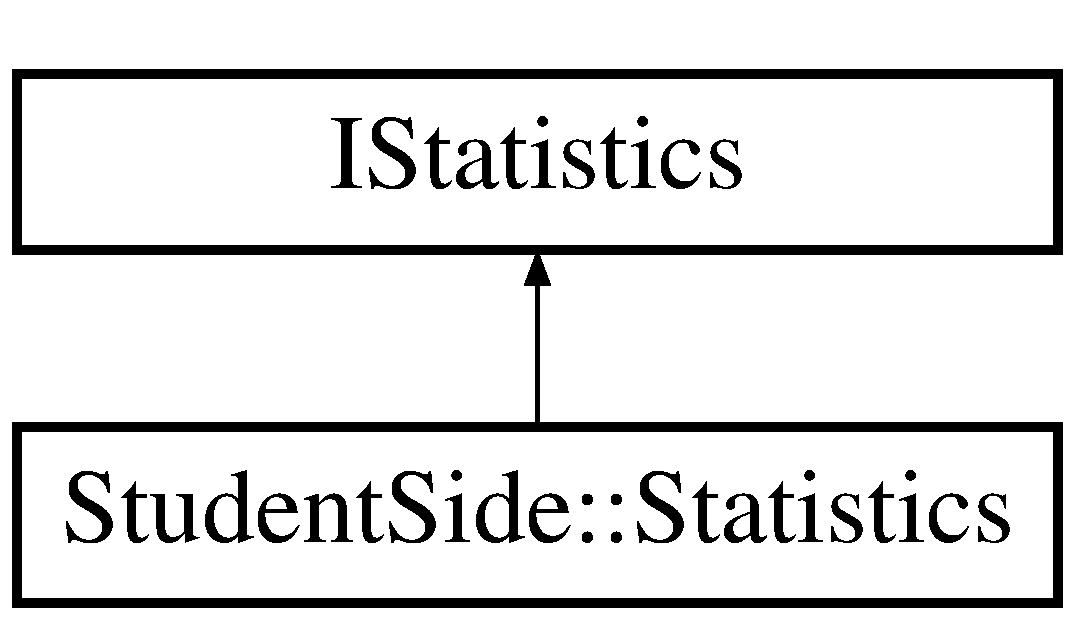
\includegraphics[height=2.000000cm]{class_student_side_1_1_statistics}
\end{center}
\end{figure}
\subsection*{Public Member Functions}
\begin{DoxyCompactItemize}
\item 
\hyperlink{class_student_side_1_1_statistics_a72567fde7744c67397c116f16fe57aed}{Statistics} ()
\begin{DoxyCompactList}\small\item\em \hyperlink{class_student_side_1_1_statistics}{Statistics} contructor. \end{DoxyCompactList}\item 
\hyperlink{class_student_side_1_1_statistics_aa49cd3fc5b2a5c4de8eea5ed690ffb77}{$\sim$\-Statistics} ()
\begin{DoxyCompactList}\small\item\em Destructor. \end{DoxyCompactList}\item 
void \hyperlink{class_student_side_1_1_statistics_a28c61977ebb56858f1cfe02ea58e22a5}{more\-Passengers} (int num) override
\begin{DoxyCompactList}\small\item\em Notifies for the player if new passengers have been added to the game. \end{DoxyCompactList}\item 
void \hyperlink{class_student_side_1_1_statistics_a95d0c05379ea6127c5d60b329e57bb97}{nysse\-Removed} () override
\begin{DoxyCompactList}\small\item\em Notifies for the player if nysse has been removed. \end{DoxyCompactList}\item 
void \hyperlink{class_student_side_1_1_statistics_af7fbe87b0c1ae4bab650ba8c53a3f677}{new\-Nysse} () override
\begin{DoxyCompactList}\small\item\em Notifies for the player if new nysse is added to the game. \end{DoxyCompactList}\item 
void \hyperlink{class_student_side_1_1_statistics_a2d7ba3c86539914571f493736d274ef0}{nysse\-Left} () override
\begin{DoxyCompactList}\small\item\em Notifies for the player if nysse has left the game area. \end{DoxyCompactList}\item 
void \hyperlink{class_student_side_1_1_statistics_ac111b2a2a9fc04b344eee9976c141d41}{Addpoints} (std\-::shared\-\_\-ptr$<$ Interface\-::\-I\-Actor $>$ actor)
\begin{DoxyCompactList}\small\item\em adds points according to which actor has been removed \end{DoxyCompactList}\item 
int \hyperlink{class_student_side_1_1_statistics_a81dff48a0178f5f66c0b01def8afd788}{give\-Current\-Points} ()
\begin{DoxyCompactList}\small\item\em gives the current points to the mainwindow \end{DoxyCompactList}\item 
int \hyperlink{class_student_side_1_1_statistics_a1578ba18299802cc369d14ea5a907a7b}{give\-Passengers} ()
\begin{DoxyCompactList}\small\item\em gives the amount of passengers removed by the player \end{DoxyCompactList}\item 
int \hyperlink{class_student_side_1_1_statistics_a55a744cc3456dad9d43679bab3b4662b}{give\-Nysses} ()
\begin{DoxyCompactList}\small\item\em gives the amount of nysses removed by the player \end{DoxyCompactList}\end{DoxyCompactItemize}


\subsection{Constructor \& Destructor Documentation}
\hypertarget{class_student_side_1_1_statistics_a72567fde7744c67397c116f16fe57aed}{\index{Student\-Side\-::\-Statistics@{Student\-Side\-::\-Statistics}!Statistics@{Statistics}}
\index{Statistics@{Statistics}!StudentSide::Statistics@{Student\-Side\-::\-Statistics}}
\subsubsection[{Statistics}]{\setlength{\rightskip}{0pt plus 5cm}Student\-Side\-::\-Statistics\-::\-Statistics (
\begin{DoxyParamCaption}
{}
\end{DoxyParamCaption}
)}}\label{class_student_side_1_1_statistics_a72567fde7744c67397c116f16fe57aed}


\hyperlink{class_student_side_1_1_statistics}{Statistics} contructor. 

\hypertarget{class_student_side_1_1_statistics_aa49cd3fc5b2a5c4de8eea5ed690ffb77}{\index{Student\-Side\-::\-Statistics@{Student\-Side\-::\-Statistics}!$\sim$\-Statistics@{$\sim$\-Statistics}}
\index{$\sim$\-Statistics@{$\sim$\-Statistics}!StudentSide::Statistics@{Student\-Side\-::\-Statistics}}
\subsubsection[{$\sim$\-Statistics}]{\setlength{\rightskip}{0pt plus 5cm}Student\-Side\-::\-Statistics\-::$\sim$\-Statistics (
\begin{DoxyParamCaption}
{}
\end{DoxyParamCaption}
)}}\label{class_student_side_1_1_statistics_aa49cd3fc5b2a5c4de8eea5ed690ffb77}


Destructor. 



\subsection{Member Function Documentation}
\hypertarget{class_student_side_1_1_statistics_ac111b2a2a9fc04b344eee9976c141d41}{\index{Student\-Side\-::\-Statistics@{Student\-Side\-::\-Statistics}!Addpoints@{Addpoints}}
\index{Addpoints@{Addpoints}!StudentSide::Statistics@{Student\-Side\-::\-Statistics}}
\subsubsection[{Addpoints}]{\setlength{\rightskip}{0pt plus 5cm}void Student\-Side\-::\-Statistics\-::\-Addpoints (
\begin{DoxyParamCaption}
\item[{std\-::shared\-\_\-ptr$<$ Interface\-::\-I\-Actor $>$}]{actor}
\end{DoxyParamCaption}
)}}\label{class_student_side_1_1_statistics_ac111b2a2a9fc04b344eee9976c141d41}


adds points according to which actor has been removed 


\begin{DoxyParams}{Parameters}
{\em actor} & Sharedpointer to Interface of \hyperlink{class_student_side_1_1_actor}{Actor} \\
\hline
\end{DoxyParams}
\begin{DoxyPrecond}{Precondition}
actor is not nullptr 
\end{DoxyPrecond}
\begin{DoxyPostcond}{Postcondition}
Exception guaranteed\-: nothrow 
\end{DoxyPostcond}
\hypertarget{class_student_side_1_1_statistics_a81dff48a0178f5f66c0b01def8afd788}{\index{Student\-Side\-::\-Statistics@{Student\-Side\-::\-Statistics}!give\-Current\-Points@{give\-Current\-Points}}
\index{give\-Current\-Points@{give\-Current\-Points}!StudentSide::Statistics@{Student\-Side\-::\-Statistics}}
\subsubsection[{give\-Current\-Points}]{\setlength{\rightskip}{0pt plus 5cm}int Student\-Side\-::\-Statistics\-::give\-Current\-Points (
\begin{DoxyParamCaption}
{}
\end{DoxyParamCaption}
)}}\label{class_student_side_1_1_statistics_a81dff48a0178f5f66c0b01def8afd788}


gives the current points to the mainwindow 

\begin{DoxyReturn}{Returns}
amount of points saved in variable points 
\end{DoxyReturn}
\begin{DoxyPrecond}{Precondition}
-\/ 
\end{DoxyPrecond}
\begin{DoxyPostcond}{Postcondition}
Exception guaranteed\-: basic 
\end{DoxyPostcond}
\hypertarget{class_student_side_1_1_statistics_a55a744cc3456dad9d43679bab3b4662b}{\index{Student\-Side\-::\-Statistics@{Student\-Side\-::\-Statistics}!give\-Nysses@{give\-Nysses}}
\index{give\-Nysses@{give\-Nysses}!StudentSide::Statistics@{Student\-Side\-::\-Statistics}}
\subsubsection[{give\-Nysses}]{\setlength{\rightskip}{0pt plus 5cm}int Student\-Side\-::\-Statistics\-::give\-Nysses (
\begin{DoxyParamCaption}
{}
\end{DoxyParamCaption}
)}}\label{class_student_side_1_1_statistics_a55a744cc3456dad9d43679bab3b4662b}


gives the amount of nysses removed by the player 

\begin{DoxyReturn}{Returns}
the amount of passengers saved in nysses 
\end{DoxyReturn}
\begin{DoxyPrecond}{Precondition}
-\/ 
\end{DoxyPrecond}
\begin{DoxyPostcond}{Postcondition}
Exception guaranteed\-: basic 
\end{DoxyPostcond}
\hypertarget{class_student_side_1_1_statistics_a1578ba18299802cc369d14ea5a907a7b}{\index{Student\-Side\-::\-Statistics@{Student\-Side\-::\-Statistics}!give\-Passengers@{give\-Passengers}}
\index{give\-Passengers@{give\-Passengers}!StudentSide::Statistics@{Student\-Side\-::\-Statistics}}
\subsubsection[{give\-Passengers}]{\setlength{\rightskip}{0pt plus 5cm}int Student\-Side\-::\-Statistics\-::give\-Passengers (
\begin{DoxyParamCaption}
{}
\end{DoxyParamCaption}
)}}\label{class_student_side_1_1_statistics_a1578ba18299802cc369d14ea5a907a7b}


gives the amount of passengers removed by the player 

\begin{DoxyReturn}{Returns}
the amount of passengers saved in passengers 
\end{DoxyReturn}
\begin{DoxyPrecond}{Precondition}
-\/ 
\end{DoxyPrecond}
\begin{DoxyPostcond}{Postcondition}
Exception guaranteed\-: basic 
\end{DoxyPostcond}
\hypertarget{class_student_side_1_1_statistics_a28c61977ebb56858f1cfe02ea58e22a5}{\index{Student\-Side\-::\-Statistics@{Student\-Side\-::\-Statistics}!more\-Passengers@{more\-Passengers}}
\index{more\-Passengers@{more\-Passengers}!StudentSide::Statistics@{Student\-Side\-::\-Statistics}}
\subsubsection[{more\-Passengers}]{\setlength{\rightskip}{0pt plus 5cm}void Student\-Side\-::\-Statistics\-::more\-Passengers (
\begin{DoxyParamCaption}
\item[{int}]{num}
\end{DoxyParamCaption}
)\hspace{0.3cm}{\ttfamily [override]}}}\label{class_student_side_1_1_statistics_a28c61977ebb56858f1cfe02ea58e22a5}


Notifies for the player if new passengers have been added to the game. 


\begin{DoxyParams}{Parameters}
{\em num} & Number of passengers in the map \\
\hline
\end{DoxyParams}
\begin{DoxyPrecond}{Precondition}
num must be positive value above zero 
\end{DoxyPrecond}
\begin{DoxyPostcond}{Postcondition}
Exception guaranteed\-: nothrow 
\end{DoxyPostcond}
\hypertarget{class_student_side_1_1_statistics_af7fbe87b0c1ae4bab650ba8c53a3f677}{\index{Student\-Side\-::\-Statistics@{Student\-Side\-::\-Statistics}!new\-Nysse@{new\-Nysse}}
\index{new\-Nysse@{new\-Nysse}!StudentSide::Statistics@{Student\-Side\-::\-Statistics}}
\subsubsection[{new\-Nysse}]{\setlength{\rightskip}{0pt plus 5cm}void Student\-Side\-::\-Statistics\-::new\-Nysse (
\begin{DoxyParamCaption}
{}
\end{DoxyParamCaption}
)\hspace{0.3cm}{\ttfamily [override]}}}\label{class_student_side_1_1_statistics_af7fbe87b0c1ae4bab650ba8c53a3f677}


Notifies for the player if new nysse is added to the game. 

\begin{DoxyPrecond}{Precondition}
-\/ 
\end{DoxyPrecond}
\begin{DoxyPostcond}{Postcondition}
Exception guaranteed\-: nothrow 
\end{DoxyPostcond}
\hypertarget{class_student_side_1_1_statistics_a2d7ba3c86539914571f493736d274ef0}{\index{Student\-Side\-::\-Statistics@{Student\-Side\-::\-Statistics}!nysse\-Left@{nysse\-Left}}
\index{nysse\-Left@{nysse\-Left}!StudentSide::Statistics@{Student\-Side\-::\-Statistics}}
\subsubsection[{nysse\-Left}]{\setlength{\rightskip}{0pt plus 5cm}void Student\-Side\-::\-Statistics\-::nysse\-Left (
\begin{DoxyParamCaption}
{}
\end{DoxyParamCaption}
)\hspace{0.3cm}{\ttfamily [override]}}}\label{class_student_side_1_1_statistics_a2d7ba3c86539914571f493736d274ef0}


Notifies for the player if nysse has left the game area. 

\begin{DoxyPrecond}{Precondition}
-\/ 
\end{DoxyPrecond}
\begin{DoxyPostcond}{Postcondition}
Exception guaranteed\-: nothrow 
\end{DoxyPostcond}
\hypertarget{class_student_side_1_1_statistics_a95d0c05379ea6127c5d60b329e57bb97}{\index{Student\-Side\-::\-Statistics@{Student\-Side\-::\-Statistics}!nysse\-Removed@{nysse\-Removed}}
\index{nysse\-Removed@{nysse\-Removed}!StudentSide::Statistics@{Student\-Side\-::\-Statistics}}
\subsubsection[{nysse\-Removed}]{\setlength{\rightskip}{0pt plus 5cm}void Student\-Side\-::\-Statistics\-::nysse\-Removed (
\begin{DoxyParamCaption}
{}
\end{DoxyParamCaption}
)\hspace{0.3cm}{\ttfamily [override]}}}\label{class_student_side_1_1_statistics_a95d0c05379ea6127c5d60b329e57bb97}


Notifies for the player if nysse has been removed. 

\begin{DoxyPrecond}{Precondition}
-\/ 
\end{DoxyPrecond}
\begin{DoxyPostcond}{Postcondition}
Exception guaranteed\-: nothrow 
\end{DoxyPostcond}


The documentation for this class was generated from the following files\-:\begin{DoxyCompactItemize}
\item 
Game/\hyperlink{statistics_8hh}{statistics.\-hh}\item 
Game/\hyperlink{statistics_8cpp}{statistics.\-cpp}\end{DoxyCompactItemize}

\hypertarget{class_ui___dialog_game_settings}{\section{Ui\-\_\-\-Dialog\-Game\-Settings Class Reference}
\label{class_ui___dialog_game_settings}\index{Ui\-\_\-\-Dialog\-Game\-Settings@{Ui\-\_\-\-Dialog\-Game\-Settings}}
}


{\ttfamily \#include $<$ui\-\_\-dialoggamesettings.\-h$>$}

Inheritance diagram for Ui\-\_\-\-Dialog\-Game\-Settings\-:\begin{figure}[H]
\begin{center}
\leavevmode
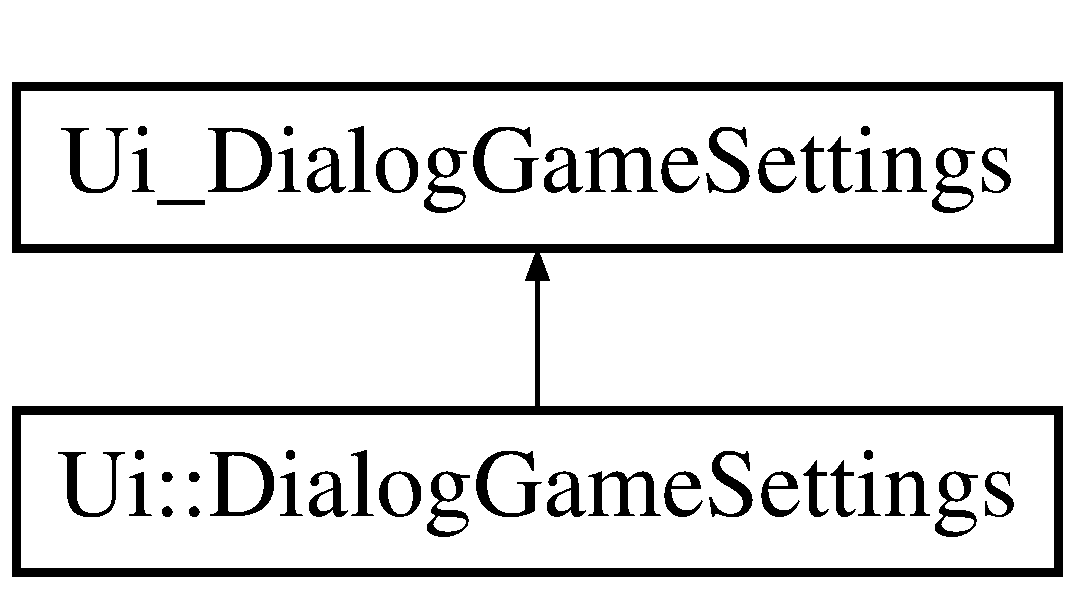
\includegraphics[height=2.000000cm]{class_ui___dialog_game_settings}
\end{center}
\end{figure}
\subsection*{Public Member Functions}
\begin{DoxyCompactItemize}
\item 
void \hyperlink{class_ui___dialog_game_settings_a454d2186fc33a40b3808cecd029cedf5}{setup\-Ui} (Q\-Dialog $\ast$Dialog\-Game\-Settings)
\item 
void \hyperlink{class_ui___dialog_game_settings_af278c61b6f1e7223bd6a9fe9bbd0b331}{retranslate\-Ui} (Q\-Dialog $\ast$Dialog\-Game\-Settings)
\end{DoxyCompactItemize}
\subsection*{Public Attributes}
\begin{DoxyCompactItemize}
\item 
Q\-Push\-Button $\ast$ \hyperlink{class_ui___dialog_game_settings_a40ae5b6fb421789d7586b3f4988eada7}{normal\-Game\-Button}
\item 
Q\-Push\-Button $\ast$ \hyperlink{class_ui___dialog_game_settings_a283359b60692817ea7b7099dde4b5fd5}{infinite\-Game\-Button}
\item 
Q\-Label $\ast$ \hyperlink{class_ui___dialog_game_settings_a133d7ca29a48667080c9110ecbe2d700}{label}
\item 
Q\-Label $\ast$ \hyperlink{class_ui___dialog_game_settings_acd81adc6c389863807a80eaa648914fa}{label\-\_\-2}
\item 
Q\-Label $\ast$ \hyperlink{class_ui___dialog_game_settings_a8d29fcac63609c2780a1ed61d40f7597}{label\-\_\-3}
\item 
Q\-Line\-Edit $\ast$ \hyperlink{class_ui___dialog_game_settings_a742bcceb2e255a8dd0916aa91510a6ce}{line\-Edit}
\item 
Q\-Check\-Box $\ast$ \hyperlink{class_ui___dialog_game_settings_a2144e6c4c4c36806ab244689d5ad29b1}{check\-Box1min}
\item 
Q\-Check\-Box $\ast$ \hyperlink{class_ui___dialog_game_settings_af65933a6ca19450ec9d170436d7d4024}{check\-Box2min}
\item 
Q\-Label $\ast$ \hyperlink{class_ui___dialog_game_settings_a29b446cc3b25e8f886ffb8f3a3917ca9}{label\-\_\-4}
\end{DoxyCompactItemize}


\subsection{Member Function Documentation}
\hypertarget{class_ui___dialog_game_settings_af278c61b6f1e7223bd6a9fe9bbd0b331}{\index{Ui\-\_\-\-Dialog\-Game\-Settings@{Ui\-\_\-\-Dialog\-Game\-Settings}!retranslate\-Ui@{retranslate\-Ui}}
\index{retranslate\-Ui@{retranslate\-Ui}!Ui_DialogGameSettings@{Ui\-\_\-\-Dialog\-Game\-Settings}}
\subsubsection[{retranslate\-Ui}]{\setlength{\rightskip}{0pt plus 5cm}void Ui\-\_\-\-Dialog\-Game\-Settings\-::retranslate\-Ui (
\begin{DoxyParamCaption}
\item[{Q\-Dialog $\ast$}]{Dialog\-Game\-Settings}
\end{DoxyParamCaption}
)\hspace{0.3cm}{\ttfamily [inline]}}}\label{class_ui___dialog_game_settings_af278c61b6f1e7223bd6a9fe9bbd0b331}
\hypertarget{class_ui___dialog_game_settings_a454d2186fc33a40b3808cecd029cedf5}{\index{Ui\-\_\-\-Dialog\-Game\-Settings@{Ui\-\_\-\-Dialog\-Game\-Settings}!setup\-Ui@{setup\-Ui}}
\index{setup\-Ui@{setup\-Ui}!Ui_DialogGameSettings@{Ui\-\_\-\-Dialog\-Game\-Settings}}
\subsubsection[{setup\-Ui}]{\setlength{\rightskip}{0pt plus 5cm}void Ui\-\_\-\-Dialog\-Game\-Settings\-::setup\-Ui (
\begin{DoxyParamCaption}
\item[{Q\-Dialog $\ast$}]{Dialog\-Game\-Settings}
\end{DoxyParamCaption}
)\hspace{0.3cm}{\ttfamily [inline]}}}\label{class_ui___dialog_game_settings_a454d2186fc33a40b3808cecd029cedf5}


\subsection{Member Data Documentation}
\hypertarget{class_ui___dialog_game_settings_a2144e6c4c4c36806ab244689d5ad29b1}{\index{Ui\-\_\-\-Dialog\-Game\-Settings@{Ui\-\_\-\-Dialog\-Game\-Settings}!check\-Box1min@{check\-Box1min}}
\index{check\-Box1min@{check\-Box1min}!Ui_DialogGameSettings@{Ui\-\_\-\-Dialog\-Game\-Settings}}
\subsubsection[{check\-Box1min}]{\setlength{\rightskip}{0pt plus 5cm}Q\-Check\-Box$\ast$ Ui\-\_\-\-Dialog\-Game\-Settings\-::check\-Box1min}}\label{class_ui___dialog_game_settings_a2144e6c4c4c36806ab244689d5ad29b1}
\hypertarget{class_ui___dialog_game_settings_af65933a6ca19450ec9d170436d7d4024}{\index{Ui\-\_\-\-Dialog\-Game\-Settings@{Ui\-\_\-\-Dialog\-Game\-Settings}!check\-Box2min@{check\-Box2min}}
\index{check\-Box2min@{check\-Box2min}!Ui_DialogGameSettings@{Ui\-\_\-\-Dialog\-Game\-Settings}}
\subsubsection[{check\-Box2min}]{\setlength{\rightskip}{0pt plus 5cm}Q\-Check\-Box$\ast$ Ui\-\_\-\-Dialog\-Game\-Settings\-::check\-Box2min}}\label{class_ui___dialog_game_settings_af65933a6ca19450ec9d170436d7d4024}
\hypertarget{class_ui___dialog_game_settings_a283359b60692817ea7b7099dde4b5fd5}{\index{Ui\-\_\-\-Dialog\-Game\-Settings@{Ui\-\_\-\-Dialog\-Game\-Settings}!infinite\-Game\-Button@{infinite\-Game\-Button}}
\index{infinite\-Game\-Button@{infinite\-Game\-Button}!Ui_DialogGameSettings@{Ui\-\_\-\-Dialog\-Game\-Settings}}
\subsubsection[{infinite\-Game\-Button}]{\setlength{\rightskip}{0pt plus 5cm}Q\-Push\-Button$\ast$ Ui\-\_\-\-Dialog\-Game\-Settings\-::infinite\-Game\-Button}}\label{class_ui___dialog_game_settings_a283359b60692817ea7b7099dde4b5fd5}
\hypertarget{class_ui___dialog_game_settings_a133d7ca29a48667080c9110ecbe2d700}{\index{Ui\-\_\-\-Dialog\-Game\-Settings@{Ui\-\_\-\-Dialog\-Game\-Settings}!label@{label}}
\index{label@{label}!Ui_DialogGameSettings@{Ui\-\_\-\-Dialog\-Game\-Settings}}
\subsubsection[{label}]{\setlength{\rightskip}{0pt plus 5cm}Q\-Label$\ast$ Ui\-\_\-\-Dialog\-Game\-Settings\-::label}}\label{class_ui___dialog_game_settings_a133d7ca29a48667080c9110ecbe2d700}
\hypertarget{class_ui___dialog_game_settings_acd81adc6c389863807a80eaa648914fa}{\index{Ui\-\_\-\-Dialog\-Game\-Settings@{Ui\-\_\-\-Dialog\-Game\-Settings}!label\-\_\-2@{label\-\_\-2}}
\index{label\-\_\-2@{label\-\_\-2}!Ui_DialogGameSettings@{Ui\-\_\-\-Dialog\-Game\-Settings}}
\subsubsection[{label\-\_\-2}]{\setlength{\rightskip}{0pt plus 5cm}Q\-Label$\ast$ Ui\-\_\-\-Dialog\-Game\-Settings\-::label\-\_\-2}}\label{class_ui___dialog_game_settings_acd81adc6c389863807a80eaa648914fa}
\hypertarget{class_ui___dialog_game_settings_a8d29fcac63609c2780a1ed61d40f7597}{\index{Ui\-\_\-\-Dialog\-Game\-Settings@{Ui\-\_\-\-Dialog\-Game\-Settings}!label\-\_\-3@{label\-\_\-3}}
\index{label\-\_\-3@{label\-\_\-3}!Ui_DialogGameSettings@{Ui\-\_\-\-Dialog\-Game\-Settings}}
\subsubsection[{label\-\_\-3}]{\setlength{\rightskip}{0pt plus 5cm}Q\-Label$\ast$ Ui\-\_\-\-Dialog\-Game\-Settings\-::label\-\_\-3}}\label{class_ui___dialog_game_settings_a8d29fcac63609c2780a1ed61d40f7597}
\hypertarget{class_ui___dialog_game_settings_a29b446cc3b25e8f886ffb8f3a3917ca9}{\index{Ui\-\_\-\-Dialog\-Game\-Settings@{Ui\-\_\-\-Dialog\-Game\-Settings}!label\-\_\-4@{label\-\_\-4}}
\index{label\-\_\-4@{label\-\_\-4}!Ui_DialogGameSettings@{Ui\-\_\-\-Dialog\-Game\-Settings}}
\subsubsection[{label\-\_\-4}]{\setlength{\rightskip}{0pt plus 5cm}Q\-Label$\ast$ Ui\-\_\-\-Dialog\-Game\-Settings\-::label\-\_\-4}}\label{class_ui___dialog_game_settings_a29b446cc3b25e8f886ffb8f3a3917ca9}
\hypertarget{class_ui___dialog_game_settings_a742bcceb2e255a8dd0916aa91510a6ce}{\index{Ui\-\_\-\-Dialog\-Game\-Settings@{Ui\-\_\-\-Dialog\-Game\-Settings}!line\-Edit@{line\-Edit}}
\index{line\-Edit@{line\-Edit}!Ui_DialogGameSettings@{Ui\-\_\-\-Dialog\-Game\-Settings}}
\subsubsection[{line\-Edit}]{\setlength{\rightskip}{0pt plus 5cm}Q\-Line\-Edit$\ast$ Ui\-\_\-\-Dialog\-Game\-Settings\-::line\-Edit}}\label{class_ui___dialog_game_settings_a742bcceb2e255a8dd0916aa91510a6ce}
\hypertarget{class_ui___dialog_game_settings_a40ae5b6fb421789d7586b3f4988eada7}{\index{Ui\-\_\-\-Dialog\-Game\-Settings@{Ui\-\_\-\-Dialog\-Game\-Settings}!normal\-Game\-Button@{normal\-Game\-Button}}
\index{normal\-Game\-Button@{normal\-Game\-Button}!Ui_DialogGameSettings@{Ui\-\_\-\-Dialog\-Game\-Settings}}
\subsubsection[{normal\-Game\-Button}]{\setlength{\rightskip}{0pt plus 5cm}Q\-Push\-Button$\ast$ Ui\-\_\-\-Dialog\-Game\-Settings\-::normal\-Game\-Button}}\label{class_ui___dialog_game_settings_a40ae5b6fb421789d7586b3f4988eada7}


The documentation for this class was generated from the following file\-:\begin{DoxyCompactItemize}
\item 
Game/\hyperlink{ui__dialoggamesettings_8h}{ui\-\_\-dialoggamesettings.\-h}\end{DoxyCompactItemize}

\hypertarget{class_ui___main_window}{\section{Ui\-\_\-\-Main\-Window Class Reference}
\label{class_ui___main_window}\index{Ui\-\_\-\-Main\-Window@{Ui\-\_\-\-Main\-Window}}
}


{\ttfamily \#include $<$ui\-\_\-mainwindow.\-h$>$}

Inheritance diagram for Ui\-\_\-\-Main\-Window\-:\begin{figure}[H]
\begin{center}
\leavevmode
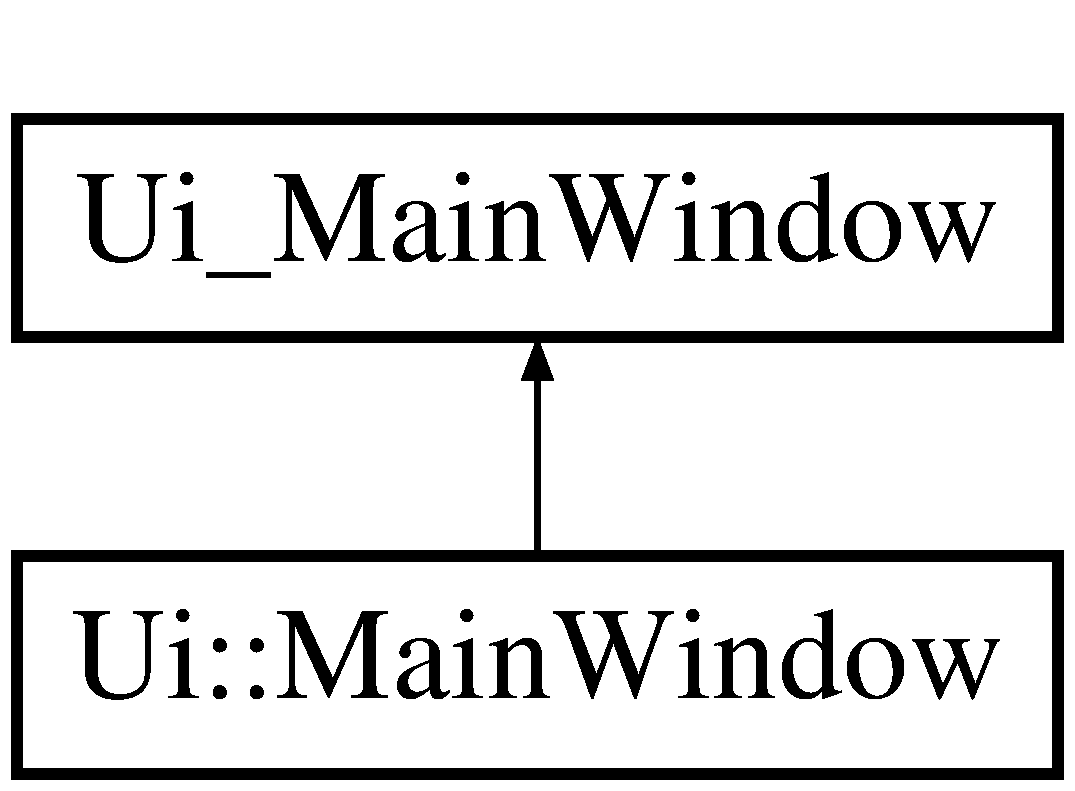
\includegraphics[height=2.000000cm]{class_ui___main_window}
\end{center}
\end{figure}
\subsection*{Public Member Functions}
\begin{DoxyCompactItemize}
\item 
void \hyperlink{class_ui___main_window_acf4a0872c4c77d8f43a2ec66ed849b58}{setup\-Ui} (Q\-Main\-Window $\ast$Main\-Window)
\item 
void \hyperlink{class_ui___main_window_a097dd160c3534a204904cb374412c618}{retranslate\-Ui} (Q\-Main\-Window $\ast$Main\-Window)
\end{DoxyCompactItemize}
\subsection*{Public Attributes}
\begin{DoxyCompactItemize}
\item 
Q\-Widget $\ast$ \hyperlink{class_ui___main_window_a356f1cf3ebda15f1fac59467ee081b74}{centralwidget}
\item 
Q\-Graphics\-View $\ast$ \hyperlink{class_ui___main_window_ae663973f203ce9ab1eeb16a5f447f01b}{game\-View}
\item 
Q\-Push\-Button $\ast$ \hyperlink{class_ui___main_window_a58a84cd3057ab5459819f986b08942b1}{start\-Button}
\item 
Q\-Label $\ast$ \hyperlink{class_ui___main_window_a134047926bc9eaff33275117ccbc9c21}{name\-Label}
\item 
Q\-Label $\ast$ \hyperlink{class_ui___main_window_a8108589cee0e2111790181434554d5e1}{playername\-Label}
\item 
Q\-L\-C\-D\-Number $\ast$ \hyperlink{class_ui___main_window_aae00401f91a31bfd7c9c7a7cee380470}{time\-\_\-lcd\-\_\-sec}
\item 
Q\-Label $\ast$ \hyperlink{class_ui___main_window_a1c286339fffe4e58accecda69001e9f5}{time\-Label}
\item 
Q\-L\-C\-D\-Number $\ast$ \hyperlink{class_ui___main_window_a390cfc326ededa1ee82c3b060e54b9f6}{time\-\_\-lcd\-\_\-min}
\item 
Q\-L\-C\-D\-Number $\ast$ \hyperlink{class_ui___main_window_aadc178326d913f4a3278657e4cde7ec6}{points\-\_\-lcd}
\item 
Q\-Label $\ast$ \hyperlink{class_ui___main_window_a8e83ba27be2971366897c2a1384d00a7}{points\-Label}
\item 
Q\-Label $\ast$ \hyperlink{class_ui___main_window_a8a23892e3dfd6fb1915c36dc3cbedeb7}{people\-Label}
\item 
Q\-L\-C\-D\-Number $\ast$ \hyperlink{class_ui___main_window_af83ee7f5b0f81925e4b6050ac03786a5}{people\-Lcd}
\item 
Q\-L\-C\-D\-Number $\ast$ \hyperlink{class_ui___main_window_aa5a21b4a3f6c07e5a7966c453ded132c}{bus\-Lcd}
\item 
Q\-Label $\ast$ \hyperlink{class_ui___main_window_ad6aa0aabd2b7ea587a730d7507eb3a33}{bus\-Label}
\item 
Q\-Menu\-Bar $\ast$ \hyperlink{class_ui___main_window_adf43d9a67adaec750aaa956b5e082f09}{menubar}
\item 
Q\-Status\-Bar $\ast$ \hyperlink{class_ui___main_window_a1687cceb1e2787aa1f83e50433943a91}{statusbar}
\end{DoxyCompactItemize}


\subsection{Member Function Documentation}
\hypertarget{class_ui___main_window_a097dd160c3534a204904cb374412c618}{\index{Ui\-\_\-\-Main\-Window@{Ui\-\_\-\-Main\-Window}!retranslate\-Ui@{retranslate\-Ui}}
\index{retranslate\-Ui@{retranslate\-Ui}!Ui_MainWindow@{Ui\-\_\-\-Main\-Window}}
\subsubsection[{retranslate\-Ui}]{\setlength{\rightskip}{0pt plus 5cm}void Ui\-\_\-\-Main\-Window\-::retranslate\-Ui (
\begin{DoxyParamCaption}
\item[{Q\-Main\-Window $\ast$}]{Main\-Window}
\end{DoxyParamCaption}
)\hspace{0.3cm}{\ttfamily [inline]}}}\label{class_ui___main_window_a097dd160c3534a204904cb374412c618}
\hypertarget{class_ui___main_window_acf4a0872c4c77d8f43a2ec66ed849b58}{\index{Ui\-\_\-\-Main\-Window@{Ui\-\_\-\-Main\-Window}!setup\-Ui@{setup\-Ui}}
\index{setup\-Ui@{setup\-Ui}!Ui_MainWindow@{Ui\-\_\-\-Main\-Window}}
\subsubsection[{setup\-Ui}]{\setlength{\rightskip}{0pt plus 5cm}void Ui\-\_\-\-Main\-Window\-::setup\-Ui (
\begin{DoxyParamCaption}
\item[{Q\-Main\-Window $\ast$}]{Main\-Window}
\end{DoxyParamCaption}
)\hspace{0.3cm}{\ttfamily [inline]}}}\label{class_ui___main_window_acf4a0872c4c77d8f43a2ec66ed849b58}


\subsection{Member Data Documentation}
\hypertarget{class_ui___main_window_ad6aa0aabd2b7ea587a730d7507eb3a33}{\index{Ui\-\_\-\-Main\-Window@{Ui\-\_\-\-Main\-Window}!bus\-Label@{bus\-Label}}
\index{bus\-Label@{bus\-Label}!Ui_MainWindow@{Ui\-\_\-\-Main\-Window}}
\subsubsection[{bus\-Label}]{\setlength{\rightskip}{0pt plus 5cm}Q\-Label$\ast$ Ui\-\_\-\-Main\-Window\-::bus\-Label}}\label{class_ui___main_window_ad6aa0aabd2b7ea587a730d7507eb3a33}
\hypertarget{class_ui___main_window_aa5a21b4a3f6c07e5a7966c453ded132c}{\index{Ui\-\_\-\-Main\-Window@{Ui\-\_\-\-Main\-Window}!bus\-Lcd@{bus\-Lcd}}
\index{bus\-Lcd@{bus\-Lcd}!Ui_MainWindow@{Ui\-\_\-\-Main\-Window}}
\subsubsection[{bus\-Lcd}]{\setlength{\rightskip}{0pt plus 5cm}Q\-L\-C\-D\-Number$\ast$ Ui\-\_\-\-Main\-Window\-::bus\-Lcd}}\label{class_ui___main_window_aa5a21b4a3f6c07e5a7966c453ded132c}
\hypertarget{class_ui___main_window_a356f1cf3ebda15f1fac59467ee081b74}{\index{Ui\-\_\-\-Main\-Window@{Ui\-\_\-\-Main\-Window}!centralwidget@{centralwidget}}
\index{centralwidget@{centralwidget}!Ui_MainWindow@{Ui\-\_\-\-Main\-Window}}
\subsubsection[{centralwidget}]{\setlength{\rightskip}{0pt plus 5cm}Q\-Widget$\ast$ Ui\-\_\-\-Main\-Window\-::centralwidget}}\label{class_ui___main_window_a356f1cf3ebda15f1fac59467ee081b74}
\hypertarget{class_ui___main_window_ae663973f203ce9ab1eeb16a5f447f01b}{\index{Ui\-\_\-\-Main\-Window@{Ui\-\_\-\-Main\-Window}!game\-View@{game\-View}}
\index{game\-View@{game\-View}!Ui_MainWindow@{Ui\-\_\-\-Main\-Window}}
\subsubsection[{game\-View}]{\setlength{\rightskip}{0pt plus 5cm}Q\-Graphics\-View$\ast$ Ui\-\_\-\-Main\-Window\-::game\-View}}\label{class_ui___main_window_ae663973f203ce9ab1eeb16a5f447f01b}
\hypertarget{class_ui___main_window_adf43d9a67adaec750aaa956b5e082f09}{\index{Ui\-\_\-\-Main\-Window@{Ui\-\_\-\-Main\-Window}!menubar@{menubar}}
\index{menubar@{menubar}!Ui_MainWindow@{Ui\-\_\-\-Main\-Window}}
\subsubsection[{menubar}]{\setlength{\rightskip}{0pt plus 5cm}Q\-Menu\-Bar$\ast$ Ui\-\_\-\-Main\-Window\-::menubar}}\label{class_ui___main_window_adf43d9a67adaec750aaa956b5e082f09}
\hypertarget{class_ui___main_window_a134047926bc9eaff33275117ccbc9c21}{\index{Ui\-\_\-\-Main\-Window@{Ui\-\_\-\-Main\-Window}!name\-Label@{name\-Label}}
\index{name\-Label@{name\-Label}!Ui_MainWindow@{Ui\-\_\-\-Main\-Window}}
\subsubsection[{name\-Label}]{\setlength{\rightskip}{0pt plus 5cm}Q\-Label$\ast$ Ui\-\_\-\-Main\-Window\-::name\-Label}}\label{class_ui___main_window_a134047926bc9eaff33275117ccbc9c21}
\hypertarget{class_ui___main_window_a8a23892e3dfd6fb1915c36dc3cbedeb7}{\index{Ui\-\_\-\-Main\-Window@{Ui\-\_\-\-Main\-Window}!people\-Label@{people\-Label}}
\index{people\-Label@{people\-Label}!Ui_MainWindow@{Ui\-\_\-\-Main\-Window}}
\subsubsection[{people\-Label}]{\setlength{\rightskip}{0pt plus 5cm}Q\-Label$\ast$ Ui\-\_\-\-Main\-Window\-::people\-Label}}\label{class_ui___main_window_a8a23892e3dfd6fb1915c36dc3cbedeb7}
\hypertarget{class_ui___main_window_af83ee7f5b0f81925e4b6050ac03786a5}{\index{Ui\-\_\-\-Main\-Window@{Ui\-\_\-\-Main\-Window}!people\-Lcd@{people\-Lcd}}
\index{people\-Lcd@{people\-Lcd}!Ui_MainWindow@{Ui\-\_\-\-Main\-Window}}
\subsubsection[{people\-Lcd}]{\setlength{\rightskip}{0pt plus 5cm}Q\-L\-C\-D\-Number$\ast$ Ui\-\_\-\-Main\-Window\-::people\-Lcd}}\label{class_ui___main_window_af83ee7f5b0f81925e4b6050ac03786a5}
\hypertarget{class_ui___main_window_a8108589cee0e2111790181434554d5e1}{\index{Ui\-\_\-\-Main\-Window@{Ui\-\_\-\-Main\-Window}!playername\-Label@{playername\-Label}}
\index{playername\-Label@{playername\-Label}!Ui_MainWindow@{Ui\-\_\-\-Main\-Window}}
\subsubsection[{playername\-Label}]{\setlength{\rightskip}{0pt plus 5cm}Q\-Label$\ast$ Ui\-\_\-\-Main\-Window\-::playername\-Label}}\label{class_ui___main_window_a8108589cee0e2111790181434554d5e1}
\hypertarget{class_ui___main_window_aadc178326d913f4a3278657e4cde7ec6}{\index{Ui\-\_\-\-Main\-Window@{Ui\-\_\-\-Main\-Window}!points\-\_\-lcd@{points\-\_\-lcd}}
\index{points\-\_\-lcd@{points\-\_\-lcd}!Ui_MainWindow@{Ui\-\_\-\-Main\-Window}}
\subsubsection[{points\-\_\-lcd}]{\setlength{\rightskip}{0pt plus 5cm}Q\-L\-C\-D\-Number$\ast$ Ui\-\_\-\-Main\-Window\-::points\-\_\-lcd}}\label{class_ui___main_window_aadc178326d913f4a3278657e4cde7ec6}
\hypertarget{class_ui___main_window_a8e83ba27be2971366897c2a1384d00a7}{\index{Ui\-\_\-\-Main\-Window@{Ui\-\_\-\-Main\-Window}!points\-Label@{points\-Label}}
\index{points\-Label@{points\-Label}!Ui_MainWindow@{Ui\-\_\-\-Main\-Window}}
\subsubsection[{points\-Label}]{\setlength{\rightskip}{0pt plus 5cm}Q\-Label$\ast$ Ui\-\_\-\-Main\-Window\-::points\-Label}}\label{class_ui___main_window_a8e83ba27be2971366897c2a1384d00a7}
\hypertarget{class_ui___main_window_a58a84cd3057ab5459819f986b08942b1}{\index{Ui\-\_\-\-Main\-Window@{Ui\-\_\-\-Main\-Window}!start\-Button@{start\-Button}}
\index{start\-Button@{start\-Button}!Ui_MainWindow@{Ui\-\_\-\-Main\-Window}}
\subsubsection[{start\-Button}]{\setlength{\rightskip}{0pt plus 5cm}Q\-Push\-Button$\ast$ Ui\-\_\-\-Main\-Window\-::start\-Button}}\label{class_ui___main_window_a58a84cd3057ab5459819f986b08942b1}
\hypertarget{class_ui___main_window_a1687cceb1e2787aa1f83e50433943a91}{\index{Ui\-\_\-\-Main\-Window@{Ui\-\_\-\-Main\-Window}!statusbar@{statusbar}}
\index{statusbar@{statusbar}!Ui_MainWindow@{Ui\-\_\-\-Main\-Window}}
\subsubsection[{statusbar}]{\setlength{\rightskip}{0pt plus 5cm}Q\-Status\-Bar$\ast$ Ui\-\_\-\-Main\-Window\-::statusbar}}\label{class_ui___main_window_a1687cceb1e2787aa1f83e50433943a91}
\hypertarget{class_ui___main_window_a390cfc326ededa1ee82c3b060e54b9f6}{\index{Ui\-\_\-\-Main\-Window@{Ui\-\_\-\-Main\-Window}!time\-\_\-lcd\-\_\-min@{time\-\_\-lcd\-\_\-min}}
\index{time\-\_\-lcd\-\_\-min@{time\-\_\-lcd\-\_\-min}!Ui_MainWindow@{Ui\-\_\-\-Main\-Window}}
\subsubsection[{time\-\_\-lcd\-\_\-min}]{\setlength{\rightskip}{0pt plus 5cm}Q\-L\-C\-D\-Number$\ast$ Ui\-\_\-\-Main\-Window\-::time\-\_\-lcd\-\_\-min}}\label{class_ui___main_window_a390cfc326ededa1ee82c3b060e54b9f6}
\hypertarget{class_ui___main_window_aae00401f91a31bfd7c9c7a7cee380470}{\index{Ui\-\_\-\-Main\-Window@{Ui\-\_\-\-Main\-Window}!time\-\_\-lcd\-\_\-sec@{time\-\_\-lcd\-\_\-sec}}
\index{time\-\_\-lcd\-\_\-sec@{time\-\_\-lcd\-\_\-sec}!Ui_MainWindow@{Ui\-\_\-\-Main\-Window}}
\subsubsection[{time\-\_\-lcd\-\_\-sec}]{\setlength{\rightskip}{0pt plus 5cm}Q\-L\-C\-D\-Number$\ast$ Ui\-\_\-\-Main\-Window\-::time\-\_\-lcd\-\_\-sec}}\label{class_ui___main_window_aae00401f91a31bfd7c9c7a7cee380470}
\hypertarget{class_ui___main_window_a1c286339fffe4e58accecda69001e9f5}{\index{Ui\-\_\-\-Main\-Window@{Ui\-\_\-\-Main\-Window}!time\-Label@{time\-Label}}
\index{time\-Label@{time\-Label}!Ui_MainWindow@{Ui\-\_\-\-Main\-Window}}
\subsubsection[{time\-Label}]{\setlength{\rightskip}{0pt plus 5cm}Q\-Label$\ast$ Ui\-\_\-\-Main\-Window\-::time\-Label}}\label{class_ui___main_window_a1c286339fffe4e58accecda69001e9f5}


The documentation for this class was generated from the following file\-:\begin{DoxyCompactItemize}
\item 
Game/\hyperlink{ui__mainwindow_8h}{ui\-\_\-mainwindow.\-h}\end{DoxyCompactItemize}

\hypertarget{class_student_side_1_1_vehicle}{\section{Student\-Side\-:\-:Vehicle Class Reference}
\label{class_student_side_1_1_vehicle}\index{Student\-Side\-::\-Vehicle@{Student\-Side\-::\-Vehicle}}
}


{\ttfamily \#include $<$vehicle.\-hh$>$}

Inheritance diagram for Student\-Side\-:\-:Vehicle\-:\begin{figure}[H]
\begin{center}
\leavevmode
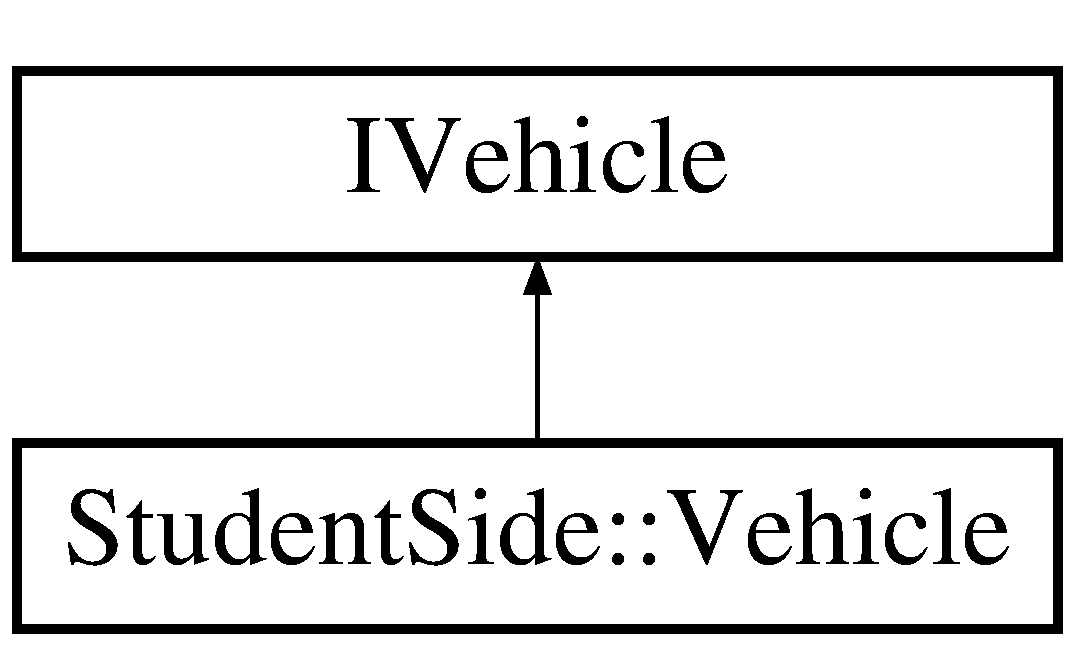
\includegraphics[height=2.000000cm]{class_student_side_1_1_vehicle}
\end{center}
\end{figure}
\subsection*{Public Member Functions}
\begin{DoxyCompactItemize}
\item 
\hyperlink{class_student_side_1_1_vehicle_a0c1ae4b0988ff51bb4ac8f3064e9eb4c}{Vehicle} ()
\begin{DoxyCompactList}\small\item\em \hyperlink{class_student_side_1_1_vehicle}{Vehicle} contructor. \end{DoxyCompactList}\item 
\hyperlink{class_student_side_1_1_vehicle_a3f7640989e79392692aa0cedaa0e4328}{$\sim$\-Vehicle} ()
\begin{DoxyCompactList}\small\item\em Destructor. \end{DoxyCompactList}\item 
std\-::string \hyperlink{class_student_side_1_1_vehicle_afc51d4f1db2c7846f471eba5b03c1d19}{get\-Name} () const override
\begin{DoxyCompactList}\small\item\em get\-Name returns the name of the vehicle \end{DoxyCompactList}\item 
std\-::vector$<$ std\-::shared\-\_\-ptr\\*
$<$ Interface\-::\-I\-Passenger $>$ $>$ \hyperlink{class_student_side_1_1_vehicle_a24c2cece6d5d46979fe9a842d72b06ed}{get\-Passengers} () const override
\begin{DoxyCompactList}\small\item\em get\-Passengers returns vector containing passengers \end{DoxyCompactList}\item 
void \hyperlink{class_student_side_1_1_vehicle_adb754d632a1cfd913adb2fb5862bf376}{add\-Passenger} (std\-::shared\-\_\-ptr$<$ Interface\-::\-I\-Passenger $>$ passenger) override
\begin{DoxyCompactList}\small\item\em add\-Passenger adds passenger to vehicle \end{DoxyCompactList}\item 
void \hyperlink{class_student_side_1_1_vehicle_a6373888a6965dbdb880d8513f9706d60}{remove\-Passenger} (std\-::shared\-\_\-ptr$<$ Interface\-::\-I\-Passenger $>$ passenger) override
\begin{DoxyCompactList}\small\item\em remove\-Passenger removes passenger form vehicle \end{DoxyCompactList}\end{DoxyCompactItemize}


\subsection{Constructor \& Destructor Documentation}
\hypertarget{class_student_side_1_1_vehicle_a0c1ae4b0988ff51bb4ac8f3064e9eb4c}{\index{Student\-Side\-::\-Vehicle@{Student\-Side\-::\-Vehicle}!Vehicle@{Vehicle}}
\index{Vehicle@{Vehicle}!StudentSide::Vehicle@{Student\-Side\-::\-Vehicle}}
\subsubsection[{Vehicle}]{\setlength{\rightskip}{0pt plus 5cm}Student\-Side\-::\-Vehicle\-::\-Vehicle (
\begin{DoxyParamCaption}
{}
\end{DoxyParamCaption}
)}}\label{class_student_side_1_1_vehicle_a0c1ae4b0988ff51bb4ac8f3064e9eb4c}


\hyperlink{class_student_side_1_1_vehicle}{Vehicle} contructor. 

\hypertarget{class_student_side_1_1_vehicle_a3f7640989e79392692aa0cedaa0e4328}{\index{Student\-Side\-::\-Vehicle@{Student\-Side\-::\-Vehicle}!$\sim$\-Vehicle@{$\sim$\-Vehicle}}
\index{$\sim$\-Vehicle@{$\sim$\-Vehicle}!StudentSide::Vehicle@{Student\-Side\-::\-Vehicle}}
\subsubsection[{$\sim$\-Vehicle}]{\setlength{\rightskip}{0pt plus 5cm}Student\-Side\-::\-Vehicle\-::$\sim$\-Vehicle (
\begin{DoxyParamCaption}
{}
\end{DoxyParamCaption}
)}}\label{class_student_side_1_1_vehicle_a3f7640989e79392692aa0cedaa0e4328}


Destructor. 



\subsection{Member Function Documentation}
\hypertarget{class_student_side_1_1_vehicle_adb754d632a1cfd913adb2fb5862bf376}{\index{Student\-Side\-::\-Vehicle@{Student\-Side\-::\-Vehicle}!add\-Passenger@{add\-Passenger}}
\index{add\-Passenger@{add\-Passenger}!StudentSide::Vehicle@{Student\-Side\-::\-Vehicle}}
\subsubsection[{add\-Passenger}]{\setlength{\rightskip}{0pt plus 5cm}void Student\-Side\-::\-Vehicle\-::add\-Passenger (
\begin{DoxyParamCaption}
\item[{std\-::shared\-\_\-ptr$<$ Interface\-::\-I\-Passenger $>$}]{passenger}
\end{DoxyParamCaption}
)\hspace{0.3cm}{\ttfamily [override]}}}\label{class_student_side_1_1_vehicle_adb754d632a1cfd913adb2fb5862bf376}


add\-Passenger adds passenger to vehicle 


\begin{DoxyParams}{Parameters}
{\em passenger} & Passenger actor \\
\hline
\end{DoxyParams}
\begin{DoxyPrecond}{Precondition}
Passenger to be added cannot be null 
\end{DoxyPrecond}
\begin{DoxyPostcond}{Postcondition}
Exception guaranteed\-: minimum 
\end{DoxyPostcond}
\hypertarget{class_student_side_1_1_vehicle_afc51d4f1db2c7846f471eba5b03c1d19}{\index{Student\-Side\-::\-Vehicle@{Student\-Side\-::\-Vehicle}!get\-Name@{get\-Name}}
\index{get\-Name@{get\-Name}!StudentSide::Vehicle@{Student\-Side\-::\-Vehicle}}
\subsubsection[{get\-Name}]{\setlength{\rightskip}{0pt plus 5cm}std\-::string Student\-Side\-::\-Vehicle\-::get\-Name (
\begin{DoxyParamCaption}
{}
\end{DoxyParamCaption}
) const\hspace{0.3cm}{\ttfamily [override]}}}\label{class_student_side_1_1_vehicle_afc51d4f1db2c7846f471eba5b03c1d19}


get\-Name returns the name of the vehicle 

\begin{DoxyReturn}{Returns}
the name of vehicle 
\end{DoxyReturn}
\begin{DoxyPrecond}{Precondition}
-\/ 
\end{DoxyPrecond}
\begin{DoxyPostcond}{Postcondition}
Exception guaranteed\-: basic 
\end{DoxyPostcond}
\hypertarget{class_student_side_1_1_vehicle_a24c2cece6d5d46979fe9a842d72b06ed}{\index{Student\-Side\-::\-Vehicle@{Student\-Side\-::\-Vehicle}!get\-Passengers@{get\-Passengers}}
\index{get\-Passengers@{get\-Passengers}!StudentSide::Vehicle@{Student\-Side\-::\-Vehicle}}
\subsubsection[{get\-Passengers}]{\setlength{\rightskip}{0pt plus 5cm}std\-::vector$<$ std\-::shared\-\_\-ptr$<$ Interface\-::\-I\-Passenger $>$ $>$ Student\-Side\-::\-Vehicle\-::get\-Passengers (
\begin{DoxyParamCaption}
{}
\end{DoxyParamCaption}
) const\hspace{0.3cm}{\ttfamily [override]}}}\label{class_student_side_1_1_vehicle_a24c2cece6d5d46979fe9a842d72b06ed}


get\-Passengers returns vector containing passengers 

\begin{DoxyReturn}{Returns}
vector containing passengers 
\end{DoxyReturn}
\begin{DoxyPrecond}{Precondition}
-\/ 
\end{DoxyPrecond}
\begin{DoxyPostcond}{Postcondition}
Exception guaranteed\-: basic 
\end{DoxyPostcond}
\hypertarget{class_student_side_1_1_vehicle_a6373888a6965dbdb880d8513f9706d60}{\index{Student\-Side\-::\-Vehicle@{Student\-Side\-::\-Vehicle}!remove\-Passenger@{remove\-Passenger}}
\index{remove\-Passenger@{remove\-Passenger}!StudentSide::Vehicle@{Student\-Side\-::\-Vehicle}}
\subsubsection[{remove\-Passenger}]{\setlength{\rightskip}{0pt plus 5cm}void Student\-Side\-::\-Vehicle\-::remove\-Passenger (
\begin{DoxyParamCaption}
\item[{std\-::shared\-\_\-ptr$<$ Interface\-::\-I\-Passenger $>$}]{passenger}
\end{DoxyParamCaption}
)\hspace{0.3cm}{\ttfamily [override]}}}\label{class_student_side_1_1_vehicle_a6373888a6965dbdb880d8513f9706d60}


remove\-Passenger removes passenger form vehicle 


\begin{DoxyParams}{Parameters}
{\em passenger} & \\
\hline
\end{DoxyParams}
\begin{DoxyPrecond}{Precondition}
Passenger to be added cannot be null 
\end{DoxyPrecond}
\begin{DoxyPostcond}{Postcondition}
Exception guaranteed\-: Strong 
\end{DoxyPostcond}


The documentation for this class was generated from the following files\-:\begin{DoxyCompactItemize}
\item 
Game/\hyperlink{vehicle_8hh}{vehicle.\-hh}\item 
Game/\hyperlink{vehicle_8cpp}{vehicle.\-cpp}\end{DoxyCompactItemize}

\chapter{File Documentation}
\hypertarget{actor_8cpp}{\section{actor.\-cpp File Reference}
\label{actor_8cpp}\index{actor.\-cpp@{actor.\-cpp}}
}
{\ttfamily \#include \char`\"{}actor.\-hh\char`\"{}}\\*
\subsection*{Namespaces}
\begin{DoxyCompactItemize}
\item 
\hyperlink{namespace_student_side}{Student\-Side}
\begin{DoxyCompactList}\small\item\em Studenside namespace. \end{DoxyCompactList}\end{DoxyCompactItemize}

\hypertarget{actor_8hh}{\section{actor.\-hh File Reference}
\label{actor_8hh}\index{actor.\-hh@{actor.\-hh}}
}


The Actor class.  


{\ttfamily \#include \char`\"{}interfaces/iactor.\-hh\char`\"{}}\\*
{\ttfamily \#include \char`\"{}core/location.\-hh\char`\"{}}\\*
{\ttfamily \#include \char`\"{}errors/gameerror.\-hh\char`\"{}}\\*
{\ttfamily \#include $<$memory$>$}\\*
\subsection*{Classes}
\begin{DoxyCompactItemize}
\item 
class \hyperlink{class_student_side_1_1_actor}{Student\-Side\-::\-Actor}
\end{DoxyCompactItemize}
\subsection*{Namespaces}
\begin{DoxyCompactItemize}
\item 
\hyperlink{namespace_student_side}{Student\-Side}
\end{DoxyCompactItemize}


\subsection{Detailed Description}
The Actor class. 
\hypertarget{actoritem_8cpp}{\section{Game/actoritem.cpp File Reference}
\label{actoritem_8cpp}\index{Game/actoritem.\-cpp@{Game/actoritem.\-cpp}}
}
{\ttfamily \#include \char`\"{}actoritem.\-hh\char`\"{}}\\*
{\ttfamily \#include $<$Q\-Debug$>$}\\*
{\ttfamily \#include $<$Q\-Image$>$}\\*
{\ttfamily \#include $<$Q\-Pixmap$>$}\\*
{\ttfamily \#include $<$assert.\-h$>$}\\*
\subsection*{Namespaces}
\begin{DoxyCompactItemize}
\item 
\hyperlink{namespace_student_side}{Student\-Side}
\begin{DoxyCompactList}\small\item\em namespace Studen\-Side, Students own imlplementations to project \end{DoxyCompactList}\end{DoxyCompactItemize}

\hypertarget{actoritem_8hh}{\section{actoritem.\-hh File Reference}
\label{actoritem_8hh}\index{actoritem.\-hh@{actoritem.\-hh}}
}


The Actor\-Item class.  


{\ttfamily \#include $<$Q\-Graphics\-Item$>$}\\*
{\ttfamily \#include $<$Q\-Graphics\-Pixmap\-Item$>$}\\*
{\ttfamily \#include $<$Q\-Graphics\-Scene$>$}\\*
{\ttfamily \#include $<$Q\-Painter$>$}\\*
\subsection*{Classes}
\begin{DoxyCompactItemize}
\item 
class \hyperlink{class_student_side_1_1_actor_item}{Student\-Side\-::\-Actor\-Item}
\end{DoxyCompactItemize}
\subsection*{Namespaces}
\begin{DoxyCompactItemize}
\item 
\hyperlink{namespace_student_side}{Student\-Side}
\end{DoxyCompactItemize}
\subsection*{Variables}
\begin{DoxyCompactItemize}
\item 
const Q\-String \hyperlink{actoritem_8hh_aa4b129297bf7c3a2ab33895c4ec37ade}{N\-Y\-S\-S\-E\-\_\-\-S\-T\-O\-P} = \char`\"{}\-:/../pics/pics/Nysse\-Stop.\-png\char`\"{}
\begin{DoxyCompactList}\small\item\em Pic of stopsign. \end{DoxyCompactList}\item 
const Q\-String \hyperlink{actoritem_8hh_aedf8524adc61b4d09d86db4fa2f207d2}{B\-U\-S\-S\-I} = \char`\"{}\-://../pics/pics/bussi.\-png\char`\"{}
\begin{DoxyCompactList}\small\item\em pic of buss \end{DoxyCompactList}\item 
const Q\-String \hyperlink{actoritem_8hh_a919ee1b297d205cded0f0dc03ade1cfd}{H\-U\-M\-A\-N} = \char`\"{}\-://../pics/pics/huma.\-png\char`\"{}
\begin{DoxyCompactList}\small\item\em pic of passenger \end{DoxyCompactList}\item 
const int \hyperlink{actoritem_8hh_abd028a1a48c574e726a4a904fff0a08c}{D\-I\-M\-\_\-\-S\-T\-O\-P} = 10
\item 
const int \hyperlink{actoritem_8hh_a0206546ca28fb9fca0c00861c5843dd5}{D\-I\-M\-\_\-\-B\-U\-S\-S} = 15
\item 
const int \hyperlink{actoritem_8hh_a94bb4115dc75d86789f2424ba4efcbdc}{D\-I\-M\-\_\-\-P\-A\-S\-S\-E\-N\-G\-E\-R} = 30
\item 
const int \hyperlink{actoritem_8hh_a65e7f70d9c573d5bfd13804a406fc067}{B\-U\-S\-S\-\_\-\-S\-T\-O\-P} = 0
\item 
const int \hyperlink{actoritem_8hh_a184d5b62435541e060c4dd4f179bec92}{N\-Y\-S\-S\-E} = 1
\item 
const int \hyperlink{actoritem_8hh_ad93711fcc7685c6b7a6530eda7984a55}{P\-A\-S\-S\-E\-N\-G\-E\-R} = 2
\item 
const int \hyperlink{actoritem_8hh_a9649ab8139c4c2ea5c93625b30d92a05}{W\-I\-D\-T\-H} = 9
\item 
const int \hyperlink{actoritem_8hh_af728b7647e0b8c49832983a31f9a2e9b}{H\-E\-I\-G\-H\-T} = 9
\end{DoxyCompactItemize}


\subsection{Detailed Description}
The Actor\-Item class. 

\subsection{Variable Documentation}
\hypertarget{actoritem_8hh_a65e7f70d9c573d5bfd13804a406fc067}{\index{actoritem.\-hh@{actoritem.\-hh}!B\-U\-S\-S\-\_\-\-S\-T\-O\-P@{B\-U\-S\-S\-\_\-\-S\-T\-O\-P}}
\index{B\-U\-S\-S\-\_\-\-S\-T\-O\-P@{B\-U\-S\-S\-\_\-\-S\-T\-O\-P}!actoritem.hh@{actoritem.\-hh}}
\subsubsection[{B\-U\-S\-S\-\_\-\-S\-T\-O\-P}]{\setlength{\rightskip}{0pt plus 5cm}const int B\-U\-S\-S\-\_\-\-S\-T\-O\-P = 0}}\label{actoritem_8hh_a65e7f70d9c573d5bfd13804a406fc067}
\hypertarget{actoritem_8hh_aedf8524adc61b4d09d86db4fa2f207d2}{\index{actoritem.\-hh@{actoritem.\-hh}!B\-U\-S\-S\-I@{B\-U\-S\-S\-I}}
\index{B\-U\-S\-S\-I@{B\-U\-S\-S\-I}!actoritem.hh@{actoritem.\-hh}}
\subsubsection[{B\-U\-S\-S\-I}]{\setlength{\rightskip}{0pt plus 5cm}const Q\-String B\-U\-S\-S\-I = \char`\"{}\-://../pics/pics/bussi.\-png\char`\"{}}}\label{actoritem_8hh_aedf8524adc61b4d09d86db4fa2f207d2}


pic of buss 

\hypertarget{actoritem_8hh_a0206546ca28fb9fca0c00861c5843dd5}{\index{actoritem.\-hh@{actoritem.\-hh}!D\-I\-M\-\_\-\-B\-U\-S\-S@{D\-I\-M\-\_\-\-B\-U\-S\-S}}
\index{D\-I\-M\-\_\-\-B\-U\-S\-S@{D\-I\-M\-\_\-\-B\-U\-S\-S}!actoritem.hh@{actoritem.\-hh}}
\subsubsection[{D\-I\-M\-\_\-\-B\-U\-S\-S}]{\setlength{\rightskip}{0pt plus 5cm}const int D\-I\-M\-\_\-\-B\-U\-S\-S = 15}}\label{actoritem_8hh_a0206546ca28fb9fca0c00861c5843dd5}
\hypertarget{actoritem_8hh_a94bb4115dc75d86789f2424ba4efcbdc}{\index{actoritem.\-hh@{actoritem.\-hh}!D\-I\-M\-\_\-\-P\-A\-S\-S\-E\-N\-G\-E\-R@{D\-I\-M\-\_\-\-P\-A\-S\-S\-E\-N\-G\-E\-R}}
\index{D\-I\-M\-\_\-\-P\-A\-S\-S\-E\-N\-G\-E\-R@{D\-I\-M\-\_\-\-P\-A\-S\-S\-E\-N\-G\-E\-R}!actoritem.hh@{actoritem.\-hh}}
\subsubsection[{D\-I\-M\-\_\-\-P\-A\-S\-S\-E\-N\-G\-E\-R}]{\setlength{\rightskip}{0pt plus 5cm}const int D\-I\-M\-\_\-\-P\-A\-S\-S\-E\-N\-G\-E\-R = 30}}\label{actoritem_8hh_a94bb4115dc75d86789f2424ba4efcbdc}
\hypertarget{actoritem_8hh_abd028a1a48c574e726a4a904fff0a08c}{\index{actoritem.\-hh@{actoritem.\-hh}!D\-I\-M\-\_\-\-S\-T\-O\-P@{D\-I\-M\-\_\-\-S\-T\-O\-P}}
\index{D\-I\-M\-\_\-\-S\-T\-O\-P@{D\-I\-M\-\_\-\-S\-T\-O\-P}!actoritem.hh@{actoritem.\-hh}}
\subsubsection[{D\-I\-M\-\_\-\-S\-T\-O\-P}]{\setlength{\rightskip}{0pt plus 5cm}const int D\-I\-M\-\_\-\-S\-T\-O\-P = 10}}\label{actoritem_8hh_abd028a1a48c574e726a4a904fff0a08c}
\hypertarget{actoritem_8hh_af728b7647e0b8c49832983a31f9a2e9b}{\index{actoritem.\-hh@{actoritem.\-hh}!H\-E\-I\-G\-H\-T@{H\-E\-I\-G\-H\-T}}
\index{H\-E\-I\-G\-H\-T@{H\-E\-I\-G\-H\-T}!actoritem.hh@{actoritem.\-hh}}
\subsubsection[{H\-E\-I\-G\-H\-T}]{\setlength{\rightskip}{0pt plus 5cm}const int H\-E\-I\-G\-H\-T = 9}}\label{actoritem_8hh_af728b7647e0b8c49832983a31f9a2e9b}
\hypertarget{actoritem_8hh_a919ee1b297d205cded0f0dc03ade1cfd}{\index{actoritem.\-hh@{actoritem.\-hh}!H\-U\-M\-A\-N@{H\-U\-M\-A\-N}}
\index{H\-U\-M\-A\-N@{H\-U\-M\-A\-N}!actoritem.hh@{actoritem.\-hh}}
\subsubsection[{H\-U\-M\-A\-N}]{\setlength{\rightskip}{0pt plus 5cm}const Q\-String H\-U\-M\-A\-N = \char`\"{}\-://../pics/pics/huma.\-png\char`\"{}}}\label{actoritem_8hh_a919ee1b297d205cded0f0dc03ade1cfd}


pic of passenger 

\hypertarget{actoritem_8hh_a184d5b62435541e060c4dd4f179bec92}{\index{actoritem.\-hh@{actoritem.\-hh}!N\-Y\-S\-S\-E@{N\-Y\-S\-S\-E}}
\index{N\-Y\-S\-S\-E@{N\-Y\-S\-S\-E}!actoritem.hh@{actoritem.\-hh}}
\subsubsection[{N\-Y\-S\-S\-E}]{\setlength{\rightskip}{0pt plus 5cm}const int N\-Y\-S\-S\-E = 1}}\label{actoritem_8hh_a184d5b62435541e060c4dd4f179bec92}
\hypertarget{actoritem_8hh_aa4b129297bf7c3a2ab33895c4ec37ade}{\index{actoritem.\-hh@{actoritem.\-hh}!N\-Y\-S\-S\-E\-\_\-\-S\-T\-O\-P@{N\-Y\-S\-S\-E\-\_\-\-S\-T\-O\-P}}
\index{N\-Y\-S\-S\-E\-\_\-\-S\-T\-O\-P@{N\-Y\-S\-S\-E\-\_\-\-S\-T\-O\-P}!actoritem.hh@{actoritem.\-hh}}
\subsubsection[{N\-Y\-S\-S\-E\-\_\-\-S\-T\-O\-P}]{\setlength{\rightskip}{0pt plus 5cm}const Q\-String N\-Y\-S\-S\-E\-\_\-\-S\-T\-O\-P = \char`\"{}\-:/../pics/pics/Nysse\-Stop.\-png\char`\"{}}}\label{actoritem_8hh_aa4b129297bf7c3a2ab33895c4ec37ade}


Pic of stopsign. 

\hypertarget{actoritem_8hh_ad93711fcc7685c6b7a6530eda7984a55}{\index{actoritem.\-hh@{actoritem.\-hh}!P\-A\-S\-S\-E\-N\-G\-E\-R@{P\-A\-S\-S\-E\-N\-G\-E\-R}}
\index{P\-A\-S\-S\-E\-N\-G\-E\-R@{P\-A\-S\-S\-E\-N\-G\-E\-R}!actoritem.hh@{actoritem.\-hh}}
\subsubsection[{P\-A\-S\-S\-E\-N\-G\-E\-R}]{\setlength{\rightskip}{0pt plus 5cm}const int P\-A\-S\-S\-E\-N\-G\-E\-R = 2}}\label{actoritem_8hh_ad93711fcc7685c6b7a6530eda7984a55}
\hypertarget{actoritem_8hh_a9649ab8139c4c2ea5c93625b30d92a05}{\index{actoritem.\-hh@{actoritem.\-hh}!W\-I\-D\-T\-H@{W\-I\-D\-T\-H}}
\index{W\-I\-D\-T\-H@{W\-I\-D\-T\-H}!actoritem.hh@{actoritem.\-hh}}
\subsubsection[{W\-I\-D\-T\-H}]{\setlength{\rightskip}{0pt plus 5cm}const int W\-I\-D\-T\-H = 9}}\label{actoritem_8hh_a9649ab8139c4c2ea5c93625b30d92a05}

\hypertarget{city_8cpp}{\section{city.\-cpp File Reference}
\label{city_8cpp}\index{city.\-cpp@{city.\-cpp}}
}
{\ttfamily \#include \char`\"{}city.\-hh\char`\"{}}\\*
{\ttfamily \#include $<$Q\-Debug$>$}\\*
{\ttfamily \#include $<$vector$>$}\\*
\subsection*{Namespaces}
\begin{DoxyCompactItemize}
\item 
\hyperlink{namespace_student_side}{Student\-Side}
\begin{DoxyCompactList}\small\item\em Studenside namespace. \end{DoxyCompactList}\end{DoxyCompactItemize}

\hypertarget{city_8hh}{\section{Game/city.hh File Reference}
\label{city_8hh}\index{Game/city.\-hh@{Game/city.\-hh}}
}


The City class that defines city operations.  


{\ttfamily \#include \char`\"{}interfaces/icity.\-hh\char`\"{}}\\*
{\ttfamily \#include \char`\"{}mainwindow.\-hh\char`\"{}}\\*
{\ttfamily \#include \char`\"{}actor.\-hh\char`\"{}}\\*
{\ttfamily \#include \char`\"{}vehicle.\-hh\char`\"{}}\\*
{\ttfamily \#include \char`\"{}statistics.\-hh\char`\"{}}\\*
{\ttfamily \#include \char`\"{}errors/gameerror.\-hh\char`\"{}}\\*
{\ttfamily \#include \char`\"{}errors/initerror.\-hh\char`\"{}}\\*
{\ttfamily \#include $<$Q\-Time$>$}\\*
{\ttfamily \#include $<$Q\-Pixmap$>$}\\*
{\ttfamily \#include $<$algorithm$>$}\\*
\subsection*{Classes}
\begin{DoxyCompactItemize}
\item 
class \hyperlink{class_student_side_1_1_city}{Student\-Side\-::\-City}
\end{DoxyCompactItemize}
\subsection*{Namespaces}
\begin{DoxyCompactItemize}
\item 
\hyperlink{namespace_student_side}{Student\-Side}
\begin{DoxyCompactList}\small\item\em namespace Studen\-Side, Students own imlplementations to project \end{DoxyCompactList}\end{DoxyCompactItemize}
\subsection*{Variables}
\begin{DoxyCompactItemize}
\item 
const int \hyperlink{city_8hh_ae64f34fc2d5f71f07cd3b6d6b9518215}{R\-E\-N\-D\-E\-R\-\_\-\-D\-I\-S\-T\-A\-N\-C\-E} = 2000
\item 
const int \hyperlink{city_8hh_ae9a58fdb539145f04f47e77582514552}{P\-A\-S\-S\-E\-N\-G\-E\-R\-\_\-\-R\-E\-N\-D\-E\-R\-\_\-\-M\-I\-N} = -\/500
\item 
const int \hyperlink{city_8hh_a96b3f3c6628cf7255e17e1b12f001e70}{P\-A\-S\-S\-E\-N\-G\-E\-R\-\_\-\-R\-E\-N\-D\-E\-R\-\_\-\-M\-A\-X} = 1050
\item 
const int \hyperlink{city_8hh_aedc95de80b52c2e078fac78e2c7a8df8}{D\-I\-S\-T\-A\-N\-C\-E\-\_\-\-T\-O\-\_\-\-I\-N\-T\-E\-R\-A\-C\-T} = 25
\end{DoxyCompactItemize}


\subsection{Detailed Description}
The City class that defines city operations. 

\subsection{Variable Documentation}
\hypertarget{city_8hh_aedc95de80b52c2e078fac78e2c7a8df8}{\index{city.\-hh@{city.\-hh}!D\-I\-S\-T\-A\-N\-C\-E\-\_\-\-T\-O\-\_\-\-I\-N\-T\-E\-R\-A\-C\-T@{D\-I\-S\-T\-A\-N\-C\-E\-\_\-\-T\-O\-\_\-\-I\-N\-T\-E\-R\-A\-C\-T}}
\index{D\-I\-S\-T\-A\-N\-C\-E\-\_\-\-T\-O\-\_\-\-I\-N\-T\-E\-R\-A\-C\-T@{D\-I\-S\-T\-A\-N\-C\-E\-\_\-\-T\-O\-\_\-\-I\-N\-T\-E\-R\-A\-C\-T}!city.hh@{city.\-hh}}
\subsubsection[{D\-I\-S\-T\-A\-N\-C\-E\-\_\-\-T\-O\-\_\-\-I\-N\-T\-E\-R\-A\-C\-T}]{\setlength{\rightskip}{0pt plus 5cm}const int D\-I\-S\-T\-A\-N\-C\-E\-\_\-\-T\-O\-\_\-\-I\-N\-T\-E\-R\-A\-C\-T = 25}}\label{city_8hh_aedc95de80b52c2e078fac78e2c7a8df8}
\hypertarget{city_8hh_a96b3f3c6628cf7255e17e1b12f001e70}{\index{city.\-hh@{city.\-hh}!P\-A\-S\-S\-E\-N\-G\-E\-R\-\_\-\-R\-E\-N\-D\-E\-R\-\_\-\-M\-A\-X@{P\-A\-S\-S\-E\-N\-G\-E\-R\-\_\-\-R\-E\-N\-D\-E\-R\-\_\-\-M\-A\-X}}
\index{P\-A\-S\-S\-E\-N\-G\-E\-R\-\_\-\-R\-E\-N\-D\-E\-R\-\_\-\-M\-A\-X@{P\-A\-S\-S\-E\-N\-G\-E\-R\-\_\-\-R\-E\-N\-D\-E\-R\-\_\-\-M\-A\-X}!city.hh@{city.\-hh}}
\subsubsection[{P\-A\-S\-S\-E\-N\-G\-E\-R\-\_\-\-R\-E\-N\-D\-E\-R\-\_\-\-M\-A\-X}]{\setlength{\rightskip}{0pt plus 5cm}const int P\-A\-S\-S\-E\-N\-G\-E\-R\-\_\-\-R\-E\-N\-D\-E\-R\-\_\-\-M\-A\-X = 1050}}\label{city_8hh_a96b3f3c6628cf7255e17e1b12f001e70}
\hypertarget{city_8hh_ae9a58fdb539145f04f47e77582514552}{\index{city.\-hh@{city.\-hh}!P\-A\-S\-S\-E\-N\-G\-E\-R\-\_\-\-R\-E\-N\-D\-E\-R\-\_\-\-M\-I\-N@{P\-A\-S\-S\-E\-N\-G\-E\-R\-\_\-\-R\-E\-N\-D\-E\-R\-\_\-\-M\-I\-N}}
\index{P\-A\-S\-S\-E\-N\-G\-E\-R\-\_\-\-R\-E\-N\-D\-E\-R\-\_\-\-M\-I\-N@{P\-A\-S\-S\-E\-N\-G\-E\-R\-\_\-\-R\-E\-N\-D\-E\-R\-\_\-\-M\-I\-N}!city.hh@{city.\-hh}}
\subsubsection[{P\-A\-S\-S\-E\-N\-G\-E\-R\-\_\-\-R\-E\-N\-D\-E\-R\-\_\-\-M\-I\-N}]{\setlength{\rightskip}{0pt plus 5cm}const int P\-A\-S\-S\-E\-N\-G\-E\-R\-\_\-\-R\-E\-N\-D\-E\-R\-\_\-\-M\-I\-N = -\/500}}\label{city_8hh_ae9a58fdb539145f04f47e77582514552}
\hypertarget{city_8hh_ae64f34fc2d5f71f07cd3b6d6b9518215}{\index{city.\-hh@{city.\-hh}!R\-E\-N\-D\-E\-R\-\_\-\-D\-I\-S\-T\-A\-N\-C\-E@{R\-E\-N\-D\-E\-R\-\_\-\-D\-I\-S\-T\-A\-N\-C\-E}}
\index{R\-E\-N\-D\-E\-R\-\_\-\-D\-I\-S\-T\-A\-N\-C\-E@{R\-E\-N\-D\-E\-R\-\_\-\-D\-I\-S\-T\-A\-N\-C\-E}!city.hh@{city.\-hh}}
\subsubsection[{R\-E\-N\-D\-E\-R\-\_\-\-D\-I\-S\-T\-A\-N\-C\-E}]{\setlength{\rightskip}{0pt plus 5cm}const int R\-E\-N\-D\-E\-R\-\_\-\-D\-I\-S\-T\-A\-N\-C\-E = 2000}}\label{city_8hh_ae64f34fc2d5f71f07cd3b6d6b9518215}

\hypertarget{creategame_8cpp}{\section{Game/creategame.cpp File Reference}
\label{creategame_8cpp}\index{Game/creategame.\-cpp@{Game/creategame.\-cpp}}
}
{\ttfamily \#include \char`\"{}creategame.\-hh\char`\"{}}\\*
{\ttfamily \#include \char`\"{}city.\-hh\char`\"{}}\\*
{\ttfamily \#include \char`\"{}Q\-Image\char`\"{}}\\*
{\ttfamily \#include $<$memory$>$}\\*

\hypertarget{dialoggamesettings_8cpp}{\section{dialoggamesettings.\-cpp File Reference}
\label{dialoggamesettings_8cpp}\index{dialoggamesettings.\-cpp@{dialoggamesettings.\-cpp}}
}
{\ttfamily \#include \char`\"{}dialoggamesettings.\-hh\char`\"{}}\\*
{\ttfamily \#include \char`\"{}ui\-\_\-dialoggamesettings.\-h\char`\"{}}\\*
\subsection*{Namespaces}
\begin{DoxyCompactItemize}
\item 
\hyperlink{namespace_student_side}{Student\-Side}
\end{DoxyCompactItemize}

\hypertarget{dialoggamesettings_8hh}{\section{Game/dialoggamesettings.hh File Reference}
\label{dialoggamesettings_8hh}\index{Game/dialoggamesettings.\-hh@{Game/dialoggamesettings.\-hh}}
}
{\ttfamily \#include $<$Q\-Dialog$>$}\\*
\subsection*{Classes}
\begin{DoxyCompactItemize}
\item 
class \hyperlink{class_student_side_1_1_dialog_game_settings}{Student\-Side\-::\-Dialog\-Game\-Settings}
\begin{DoxyCompactList}\small\item\em The Dialog\-Gane\-Settings class sets up dialog window to get pre settings for the main game. \end{DoxyCompactList}\end{DoxyCompactItemize}
\subsection*{Namespaces}
\begin{DoxyCompactItemize}
\item 
\hyperlink{namespace_ui}{Ui}
\begin{DoxyCompactList}\small\item\em namespace \hyperlink{namespace_ui}{Ui} for dialog window class \end{DoxyCompactList}\item 
\hyperlink{namespace_student_side}{Student\-Side}
\begin{DoxyCompactList}\small\item\em namespace Studen\-Side, Students own imlplementations to project \end{DoxyCompactList}\end{DoxyCompactItemize}
\subsection*{Variables}
\begin{DoxyCompactItemize}
\item 
const int \hyperlink{dialoggamesettings_8hh_a8b40e2e7fdfe4c765aa9aaa6fec9b431}{O\-N\-E\-\_\-\-M\-I\-N\-U\-T\-E} = 60
\item 
const int \hyperlink{dialoggamesettings_8hh_aedc05529ef6072630839aed27d71b5ae}{T\-W\-O\-\_\-\-M\-I\-N\-U\-T\-E} = 120
\end{DoxyCompactItemize}


\subsection{Variable Documentation}
\hypertarget{dialoggamesettings_8hh_a8b40e2e7fdfe4c765aa9aaa6fec9b431}{\index{dialoggamesettings.\-hh@{dialoggamesettings.\-hh}!O\-N\-E\-\_\-\-M\-I\-N\-U\-T\-E@{O\-N\-E\-\_\-\-M\-I\-N\-U\-T\-E}}
\index{O\-N\-E\-\_\-\-M\-I\-N\-U\-T\-E@{O\-N\-E\-\_\-\-M\-I\-N\-U\-T\-E}!dialoggamesettings.hh@{dialoggamesettings.\-hh}}
\subsubsection[{O\-N\-E\-\_\-\-M\-I\-N\-U\-T\-E}]{\setlength{\rightskip}{0pt plus 5cm}const int O\-N\-E\-\_\-\-M\-I\-N\-U\-T\-E = 60}}\label{dialoggamesettings_8hh_a8b40e2e7fdfe4c765aa9aaa6fec9b431}
\hypertarget{dialoggamesettings_8hh_aedc05529ef6072630839aed27d71b5ae}{\index{dialoggamesettings.\-hh@{dialoggamesettings.\-hh}!T\-W\-O\-\_\-\-M\-I\-N\-U\-T\-E@{T\-W\-O\-\_\-\-M\-I\-N\-U\-T\-E}}
\index{T\-W\-O\-\_\-\-M\-I\-N\-U\-T\-E@{T\-W\-O\-\_\-\-M\-I\-N\-U\-T\-E}!dialoggamesettings.hh@{dialoggamesettings.\-hh}}
\subsubsection[{T\-W\-O\-\_\-\-M\-I\-N\-U\-T\-E}]{\setlength{\rightskip}{0pt plus 5cm}const int T\-W\-O\-\_\-\-M\-I\-N\-U\-T\-E = 120}}\label{dialoggamesettings_8hh_aedc05529ef6072630839aed27d71b5ae}

\hypertarget{gameengine_8cpp}{\section{gameengine.\-cpp File Reference}
\label{gameengine_8cpp}\index{gameengine.\-cpp@{gameengine.\-cpp}}
}
{\ttfamily \#include \char`\"{}gameengine.\-hh\char`\"{}}\\*
{\ttfamily \#include \char`\"{}ui\-\_\-mainwindow.\-h\char`\"{}}\\*
{\ttfamily \#include $<$memory$>$}\\*
{\ttfamily \#include $<$Q\-Image$>$}\\*
{\ttfamily \#include $<$Q\-Debug$>$}\\*
{\ttfamily \#include $<$Q\-Object$>$}\\*
{\ttfamily \#include $<$Q\-Push\-Button$>$}\\*
\subsection*{Namespaces}
\begin{DoxyCompactItemize}
\item 
\hyperlink{namespace_student_side}{Student\-Side}
\begin{DoxyCompactList}\small\item\em Studenside namespace. \end{DoxyCompactList}\end{DoxyCompactItemize}

\hypertarget{gameengine_8hh}{\section{gameengine.\-hh File Reference}
\label{gameengine_8hh}\index{gameengine.\-hh@{gameengine.\-hh}}
}
{\ttfamily \#include \char`\"{}dialoggamesettings.\-hh\char`\"{}}\\*
{\ttfamily \#include \char`\"{}creategame.\-hh\char`\"{}}\\*
{\ttfamily \#include \char`\"{}city.\-hh\char`\"{}}\\*
{\ttfamily \#include \char`\"{}../\-Course/\-Course\-Lib/core/logic.\-hh\char`\"{}}\\*
{\ttfamily \#include $<$Q\-Image$>$}\\*
{\ttfamily \#include \char`\"{}playeractor.\-hh\char`\"{}}\\*
{\ttfamily \#include \char`\"{}Q\-Time\char`\"{}}\\*
{\ttfamily \#include \char`\"{}core/location.\-hh\char`\"{}}\\*
{\ttfamily \#include \char`\"{}statistics.\-hh\char`\"{}}\\*
{\ttfamily \#include \char`\"{}errors/initerror.\-hh\char`\"{}}\\*
\subsection*{Classes}
\begin{DoxyCompactItemize}
\item 
class \hyperlink{class_student_side_1_1_game_engine}{Student\-Side\-::\-Game\-Engine}
\begin{DoxyCompactList}\small\item\em The Init\-Game\-Engine class is for setting the game up. It launches dialog window for settings and initializes gamewindow. \end{DoxyCompactList}\end{DoxyCompactItemize}
\subsection*{Namespaces}
\begin{DoxyCompactItemize}
\item 
\hyperlink{namespace_student_side}{Student\-Side}
\end{DoxyCompactItemize}
\subsection*{Variables}
\begin{DoxyCompactItemize}
\item 
const Q\-String \hyperlink{gameengine_8hh_ad6494001dd20d6bedc7543fec6c695ba}{big\-Map} = \char`\"{}\-:/offlinedata/offlinedata/kartta\-\_\-iso\-\_\-1095x592.\-png\char`\"{}
\item 
const Q\-String \hyperlink{gameengine_8hh_af60fadacdd8d88e839ee0eae05d28518}{small\-Map} = \char`\"{}\-:/offlinedata/offlinedata/kartta\-\_\-pieni\-\_\-500x500.\-png\char`\"{}
\end{DoxyCompactItemize}


\subsection{Variable Documentation}
\hypertarget{gameengine_8hh_ad6494001dd20d6bedc7543fec6c695ba}{\index{gameengine.\-hh@{gameengine.\-hh}!big\-Map@{big\-Map}}
\index{big\-Map@{big\-Map}!gameengine.hh@{gameengine.\-hh}}
\subsubsection[{big\-Map}]{\setlength{\rightskip}{0pt plus 5cm}const Q\-String big\-Map = \char`\"{}\-:/offlinedata/offlinedata/kartta\-\_\-iso\-\_\-1095x592.\-png\char`\"{}}}\label{gameengine_8hh_ad6494001dd20d6bedc7543fec6c695ba}
\hypertarget{gameengine_8hh_af60fadacdd8d88e839ee0eae05d28518}{\index{gameengine.\-hh@{gameengine.\-hh}!small\-Map@{small\-Map}}
\index{small\-Map@{small\-Map}!gameengine.hh@{gameengine.\-hh}}
\subsubsection[{small\-Map}]{\setlength{\rightskip}{0pt plus 5cm}const Q\-String small\-Map = \char`\"{}\-:/offlinedata/offlinedata/kartta\-\_\-pieni\-\_\-500x500.\-png\char`\"{}}}\label{gameengine_8hh_af60fadacdd8d88e839ee0eae05d28518}

\hypertarget{dynsections_8js}{\section{Game/html/dynsections.js File Reference}
\label{dynsections_8js}\index{Game/html/dynsections.\-js@{Game/html/dynsections.\-js}}
}
\subsection*{Functions}
\begin{DoxyCompactItemize}
\item 
function \hyperlink{dynsections_8js_a1922c462474df7dfd18741c961d59a25}{toggle\-Visibility} (link\-Obj)
\item 
function \hyperlink{dynsections_8js_a8f7493ad859d4fbf2523917511ee7177}{update\-Stripes} ()
\item 
function \hyperlink{dynsections_8js_a19f577cc1ba571396a85bb1f48bf4df2}{toggle\-Level} (level)
\item 
function \hyperlink{dynsections_8js_af244da4527af2d845dca04f5656376cd}{toggle\-Folder} (id)
\item 
function \hyperlink{dynsections_8js_ac057b640b17ff32af11ced151c9305b4}{toggle\-Inherit} (id)
\end{DoxyCompactItemize}


\subsection{Function Documentation}
\hypertarget{dynsections_8js_af244da4527af2d845dca04f5656376cd}{\index{dynsections.\-js@{dynsections.\-js}!toggle\-Folder@{toggle\-Folder}}
\index{toggle\-Folder@{toggle\-Folder}!dynsections.js@{dynsections.\-js}}
\subsubsection[{toggle\-Folder}]{\setlength{\rightskip}{0pt plus 5cm}function toggle\-Folder (
\begin{DoxyParamCaption}
\item[{}]{id}
\end{DoxyParamCaption}
)}}\label{dynsections_8js_af244da4527af2d845dca04f5656376cd}
\hypertarget{dynsections_8js_ac057b640b17ff32af11ced151c9305b4}{\index{dynsections.\-js@{dynsections.\-js}!toggle\-Inherit@{toggle\-Inherit}}
\index{toggle\-Inherit@{toggle\-Inherit}!dynsections.js@{dynsections.\-js}}
\subsubsection[{toggle\-Inherit}]{\setlength{\rightskip}{0pt plus 5cm}function toggle\-Inherit (
\begin{DoxyParamCaption}
\item[{}]{id}
\end{DoxyParamCaption}
)}}\label{dynsections_8js_ac057b640b17ff32af11ced151c9305b4}
\hypertarget{dynsections_8js_a19f577cc1ba571396a85bb1f48bf4df2}{\index{dynsections.\-js@{dynsections.\-js}!toggle\-Level@{toggle\-Level}}
\index{toggle\-Level@{toggle\-Level}!dynsections.js@{dynsections.\-js}}
\subsubsection[{toggle\-Level}]{\setlength{\rightskip}{0pt plus 5cm}function toggle\-Level (
\begin{DoxyParamCaption}
\item[{}]{level}
\end{DoxyParamCaption}
)}}\label{dynsections_8js_a19f577cc1ba571396a85bb1f48bf4df2}
\hypertarget{dynsections_8js_a1922c462474df7dfd18741c961d59a25}{\index{dynsections.\-js@{dynsections.\-js}!toggle\-Visibility@{toggle\-Visibility}}
\index{toggle\-Visibility@{toggle\-Visibility}!dynsections.js@{dynsections.\-js}}
\subsubsection[{toggle\-Visibility}]{\setlength{\rightskip}{0pt plus 5cm}function toggle\-Visibility (
\begin{DoxyParamCaption}
\item[{}]{link\-Obj}
\end{DoxyParamCaption}
)}}\label{dynsections_8js_a1922c462474df7dfd18741c961d59a25}
\hypertarget{dynsections_8js_a8f7493ad859d4fbf2523917511ee7177}{\index{dynsections.\-js@{dynsections.\-js}!update\-Stripes@{update\-Stripes}}
\index{update\-Stripes@{update\-Stripes}!dynsections.js@{dynsections.\-js}}
\subsubsection[{update\-Stripes}]{\setlength{\rightskip}{0pt plus 5cm}function update\-Stripes (
\begin{DoxyParamCaption}
{}
\end{DoxyParamCaption}
)}}\label{dynsections_8js_a8f7493ad859d4fbf2523917511ee7177}

\hypertarget{jquery_8js}{\section{Game/html/jquery.js File Reference}
\label{jquery_8js}\index{Game/html/jquery.\-js@{Game/html/jquery.\-js}}
}
\subsection*{Functions}
\begin{DoxyCompactItemize}
\item 
\hyperlink{jquery_8js_a2fa551895933fae935a0a6b87282241d}{b} \hyperlink{jquery_8js_ad0188a1a0e382f892522cfb7dafcc937}{extend} (\{css\-Hooks\-:\{opacity\-:\{get\-:function(bw, bv)\{\hyperlink{jquery_8js_ab5582cce20b35070b73869356a852365}{if}(bv)\{var e=\hyperlink{jquery_8js_adc18d83abfd9f87d396e8fd6b6ac0fe1}{Z}(bw,\char`\"{}opacity\char`\"{},\char`\"{}opacity\char`\"{});return e===\char`\"{}\char`\"{}?\char`\"{}1\char`\"{}\-:e\}\hyperlink{jquery_8js_a0544c3fe466e421738dae463968b70ba}{else}\{return bw.\-style.\-opacity\}\}\}\}, css\-Number\-:\{fill\-Opacity\-:true, font\-Weight\-:true, line\-Height\-:true, opacity\-:true, orphans\-:true, widows\-:true, z\-Index\-:true, zoom\-:true\}, css\-Props\-:\{\char`\"{}float\char`\"{}\-:b.\-support.\-css\-Float?\char`\"{}css\-Float\char`\"{}\-:\char`\"{}style\-Float\char`\"{}\}, style\-:function(bx, bw, b\-D, by)\{\hyperlink{jquery_8js_ab5582cce20b35070b73869356a852365}{if}(!bx$|$$|$bx.\-node\-Type===3$|$$|$bx.\-node\-Type===8$|$$|$!bx.\-style)\{return\}var b\-B, b\-C, bz=b.\-camel\-Case(bw), bv=bx.\-style, b\-E=b.\-css\-Hooks\mbox{[}bz\mbox{]};bw=b.\-css\-Props\mbox{[}bz\mbox{]}$|$$|$bz;\hyperlink{jquery_8js_ab5582cce20b35070b73869356a852365}{if}(b\-D!==\hyperlink{jquery_8js_a38ee4c0b5f4fe2a18d0c783af540d253}{L})\{b\-C=typeof b\-D;\hyperlink{jquery_8js_ab5582cce20b35070b73869356a852365}{if}(b\-C===\char`\"{}string\char`\"{}\&\&(b\-B=I.\-exec(b\-D)))\{b\-D=(+(b\-B\mbox{[}1\mbox{]}+1)$\ast$+b\-B\mbox{[}2\mbox{]})+parse\-Float(\hyperlink{jquery_8js_a89ad527fcd82c01ebb587332f5b4fcd4}{b.\-css}(bx, bw));b\-C=\char`\"{}number\char`\"{}\}if(b\-D==null$|$$|$b\-C===\char`\"{}number\char`\"{}\&\&is\-Na\-N(b\-D))\{return\}\hyperlink{jquery_8js_ab5582cce20b35070b73869356a852365}{if}(b\-C===\char`\"{}number\char`\"{}\&\&!b.\-css\-Number\mbox{[}bz\mbox{]})\{b\-D+=\char`\"{}px\char`\"{}\}if(!b\-E$|$$|$!(\char`\"{}set\char`\"{}in b\-E)$|$$|$(b\-D=b\-E.\-set(bx, b\-D))!==\hyperlink{jquery_8js_a38ee4c0b5f4fe2a18d0c783af540d253}{L})\{try\{bv\mbox{[}bw\mbox{]}=b\-D\}catch(b\-A)\{\}\}\}\hyperlink{jquery_8js_a0544c3fe466e421738dae463968b70ba}{else}\{\hyperlink{jquery_8js_ab5582cce20b35070b73869356a852365}{if}(b\-E \&\&\char`\"{}get\char`\"{}in b\-E \&\&(b\-B=b\-E.\-get(bx, false, by))!==\hyperlink{jquery_8js_a38ee4c0b5f4fe2a18d0c783af540d253}{L})\{return b\-B\}return bv\mbox{[}bw\mbox{]}\}\}, css\-:function(by, bx, bv)\{var bw, e;bx=b.\-camel\-Case(bx);e=b.\-css\-Hooks\mbox{[}bx\mbox{]};bx=b.\-css\-Props\mbox{[}bx\mbox{]}$|$$|$bx;\hyperlink{jquery_8js_ab5582cce20b35070b73869356a852365}{if}(bx===\char`\"{}css\-Float\char`\"{})\{bx=\char`\"{}float\char`\"{}\}if(e \&\&\char`\"{}get\char`\"{}in e \&\&(bw=e.\-get(by, true, bv))!==\hyperlink{jquery_8js_a38ee4c0b5f4fe2a18d0c783af540d253}{L})\{return bw\}\hyperlink{jquery_8js_a0544c3fe466e421738dae463968b70ba}{else}\{\hyperlink{jquery_8js_ab5582cce20b35070b73869356a852365}{if}(\hyperlink{jquery_8js_adc18d83abfd9f87d396e8fd6b6ac0fe1}{Z})\{return \hyperlink{jquery_8js_adc18d83abfd9f87d396e8fd6b6ac0fe1}{Z}(by, bx)\}\}\}, swap\-:function(bx, bw, by)\{var e=\{\};for(var bv in bw)\{e\mbox{[}bv\mbox{]}=bx.\-style\mbox{[}bv\mbox{]};bx.\-style\mbox{[}bv\mbox{]}=bw\mbox{[}bv\mbox{]}\}by.\-call(bx);for(bv in bw)\{bx.\-style\mbox{[}bv\mbox{]}=e\mbox{[}bv\mbox{]}\}\}\})
\item 
\hyperlink{jquery_8js_a2fa551895933fae935a0a6b87282241d}{b} \hyperlink{jquery_8js_a871ff39db627c54c710a3e9909b8234c}{each} (\mbox{[}\char`\"{}height\char`\"{},\char`\"{}width\char`\"{}\mbox{]}, function(bv, e)\{b.\-css\-Hooks\mbox{[}e\mbox{]}=\{get\-:function(by, bx, bw)\{var bz;\hyperlink{jquery_8js_ab5582cce20b35070b73869356a852365}{if}(bx)\{\hyperlink{jquery_8js_ab5582cce20b35070b73869356a852365}{if}(by.\-offset\-Width!==0)\{return \hyperlink{jquery_8js_a2335e57f79b6acfb6de59c235dc8a83e}{p}(by, e, bw)\}\hyperlink{jquery_8js_a0544c3fe466e421738dae463968b70ba}{else}\{b.\-swap(by, a7, function()\{bz=\hyperlink{jquery_8js_a2335e57f79b6acfb6de59c235dc8a83e}{p}(by, e, bw)\})\}return bz\}\}, set\-:function(bw, bx)\{\hyperlink{jquery_8js_ab5582cce20b35070b73869356a852365}{if}(bc.\-test(bx))\{bx=parse\-Float(bx);\hyperlink{jquery_8js_ab5582cce20b35070b73869356a852365}{if}(bx $>$=0)\{return bx+\char`\"{}px\char`\"{}\}\}else\{return bx\}\}\}\})
\item 
\hyperlink{jquery_8js_a9db6d45a025ad692282fe23e69eeba43}{if} (!b.\-support.\-opacity)
\item 
\hyperlink{jquery_8js_a2fa551895933fae935a0a6b87282241d}{b} (function()\{\hyperlink{jquery_8js_ab5582cce20b35070b73869356a852365}{if}(!b.\-support.\-reliable\-Margin\-Right)\{b.\-css\-Hooks.\-margin\-Right=\{get\-:function(bw, bv)\{var e;b.\-swap(bw,\{display\-:\char`\"{}inline-\/block\char`\"{}\}, function()\{\hyperlink{jquery_8js_ab5582cce20b35070b73869356a852365}{if}(bv)\{e=\hyperlink{jquery_8js_adc18d83abfd9f87d396e8fd6b6ac0fe1}{Z}(bw,\char`\"{}margin-\/right\char`\"{},\char`\"{}margin\-Right\char`\"{})\}else\{e=bw.\-style.\-margin\-Right\}\});return e\}\}\}\})
\item 
\hyperlink{jquery_8js_a30d3d2cd5b567c9f31b2aa30b9cb3bb8}{if} (av.\-default\-View \&\&av.\-default\-View.\-get\-Computed\-Style)
\item 
\hyperlink{jquery_8js_a2c54bd8ed7482e89d19331ba61fe221c}{if} (av.\-document\-Element.\-current\-Style)
\item 
function \hyperlink{jquery_8js_a2335e57f79b6acfb6de59c235dc8a83e}{p} (by, bw, bv)
\item 
\hyperlink{jquery_8js_a42cbfadee2b4749e8f699ea8d745a0e4}{if} (b.\-expr \&\&b.\-expr.\-filters)
\item 
function \hyperlink{jquery_8js_a6fc9115e5c9c910cae480abf0a8c7ae3}{bh} ()
\item 
function \hyperlink{jquery_8js_a31b1c836ab707421c59d8f31b49a8f68}{at} ()
\item 
function \hyperlink{jquery_8js_ab5b2b69c05d6a629ddd1deebef38735e}{a0} (bv, e)
\item 
\hyperlink{jquery_8js_a2fa551895933fae935a0a6b87282241d}{b} \hyperlink{jquery_8js_a32214c73aa06d5951f5321466df68ad0}{each} (\{slide\-Down\-:a0(\char`\"{}show\char`\"{}, 1), slide\-Up\-:a0(\char`\"{}hide\char`\"{}, 1), slide\-Toggle\-:a0(\char`\"{}toggle\char`\"{}, 1), fade\-In\-:\{opacity\-:\char`\"{}show\char`\"{}\}, fade\-Out\-:\{opacity\-:\char`\"{}hide\char`\"{}\}, fade\-Toggle\-:\{opacity\-:\char`\"{}toggle\char`\"{}\}\}, function(e, bv)\{b.\-fn\mbox{[}e\mbox{]}=function(bw, by, bx)\{return this.\-animate(bv, bw, by, bx)\}\})
\item 
\hyperlink{jquery_8js_a2fa551895933fae935a0a6b87282241d}{b} \hyperlink{jquery_8js_aa6142183da6ef351faf36761e8a8835b}{extend} (b.\-fx,\{tick\-:function()\{var bw, bv=b.\-timers, e=0;for(;e$<$ bv.\-length;e++)\{bw=bv\mbox{[}e\mbox{]};\hyperlink{jquery_8js_ab5582cce20b35070b73869356a852365}{if}(!bw()\&\&bv\mbox{[}e\mbox{]}===bw)\{bv.\-splice(e-\/-\/, 1)\}\}\hyperlink{jquery_8js_ab5582cce20b35070b73869356a852365}{if}(!bv.\-length)\{b.\-fx.\-stop()\}\}, interval\-:13, stop\-:function()\{clear\-Interval(a3);a3=null\}, speeds\-:\{slow\-:600, fast\-:200, \-\_\-default\-:400\}, step\-:\{opacity\-:function(e)\{b.\-style(e.\-elem,\char`\"{}opacity\char`\"{}, e.\-now)\}, \-\_\-default\-:function(e)\{\hyperlink{jquery_8js_ab5582cce20b35070b73869356a852365}{if}(e.\-elem.\-style \&\&e.\-elem.\-style\mbox{[}e.\-prop\mbox{]}!=null)\{e.\-elem.\-style\mbox{[}e.\-prop\mbox{]}=e.\-now+e.\-unit\}\hyperlink{jquery_8js_a0544c3fe466e421738dae463968b70ba}{else}\{e.\-elem\mbox{[}e.\-prop\mbox{]}=e.\-now\}\}\}\})
\item 
function \hyperlink{jquery_8js_a4c3eadaa5164016d2c340d495fc6e55e}{x} (bx)
\item 
\hyperlink{jquery_8js_ad9fda9e3432e66926c2578b06f13525f}{if} (\char`\"{}get\-Bounding\-Client\-Rect\char`\"{}in av.\-document\-Element)
\item 
function \hyperlink{jquery_8js_a7d370833f2145fc5f6c371e98d754eb4}{a\-K} (e)
\item 
\hyperlink{jquery_8js_ab5582cce20b35070b73869356a852365}{if} (typeof define===\char`\"{}function\char`\"{}\&\&define.\-amd \&\&\hyperlink{jquery_8js_aa676d9980e4aff2d9210b4c8e0e1dad9}{define.\-amd.\-j\-Query})
\end{DoxyCompactItemize}
\subsection*{Variables}
\begin{DoxyCompactItemize}
\item 
function \hyperlink{jquery_8js_a1d6558865876e1c8cca029fce41a4bdb}{bb}
\item 
function \hyperlink{jquery_8js_a38ee4c0b5f4fe2a18d0c783af540d253}{L} \{var av=bb.\-document,bu=bb.\-navigator,bl=bb.\-location
\item 
var \hyperlink{jquery_8js_aa4026ad5544b958e54ce5e106fa1c805}{b}
\item 
var \hyperlink{jquery_8js_a4fd8ddfab07c8d7c7cae0ab0e052cad3}{au} =/opacity=(\mbox{[}$^\wedge$)\mbox{]}$\ast$)/,z=/(\mbox{[}A-\/\hyperlink{jquery_8js_adc18d83abfd9f87d396e8fd6b6ac0fe1}{Z}\mbox{]}$|$$^\wedge$ms)/g,bc=/$^\wedge$-\/?\textbackslash{}d+(?\-:px)?\$/i,bn=/$^\wedge$-\/?\textbackslash{}d/,I=/$^\wedge$(\mbox{[}\textbackslash{}-\/+\mbox{]})=(\mbox{[}\textbackslash{}-\/+.\textbackslash{}de\mbox{]}+)/,a7=\{position\-:\char`\"{}absolute\char`\"{},visibility\-:\char`\"{}hidden\char`\"{},display\-:\char`\"{}block\char`\"{}\},an=\mbox{[}\char`\"{}Left\char`\"{},\char`\"{}Right\char`\"{}\mbox{]},a1=\mbox{[}\char`\"{}Top\char`\"{},\char`\"{}Bottom\char`\"{}\mbox{]},Z,a\-I,a\-X
\item 
\hyperlink{jquery_8js_a2fa551895933fae935a0a6b87282241d}{b} fn \hyperlink{jquery_8js_a89ad527fcd82c01ebb587332f5b4fcd4}{css} =function(e,bv)\{\hyperlink{jquery_8js_ab5582cce20b35070b73869356a852365}{if}(arguments.\-length===2\&\&bv===\hyperlink{jquery_8js_a38ee4c0b5f4fe2a18d0c783af540d253}{L})\{return this\}return b.\-access(this,e,bv,true,function(bx,bw,by)\{return by!==\hyperlink{jquery_8js_a38ee4c0b5f4fe2a18d0c783af540d253}{L}?b.\-style(bx,bw,by)\-:b.\-css(bx,bw)\})\}
\item 
\hyperlink{jquery_8js_a2fa551895933fae935a0a6b87282241d}{b} \hyperlink{jquery_8js_a88b21f8ba3af86d6981b1da520ece33b}{cur\-C\-S\-S} =\hyperlink{jquery_8js_a89ad527fcd82c01ebb587332f5b4fcd4}{b.\-css}
\item 
\hyperlink{jquery_8js_adc18d83abfd9f87d396e8fd6b6ac0fe1}{Z} =a\-I$|$$|$a\-X
\item 
var \hyperlink{jquery_8js_ab26645c014aa005ecedef329ecf58c99}{k} =/\%20/g
\item 
var \hyperlink{jquery_8js_a6ddf393cc7f9a8828e197bb0d9916c44}{ap} =/\textbackslash{}\mbox{[}\textbackslash{}\mbox{]}\$/
\item 
var \hyperlink{jquery_8js_ae77642f8ef73fb9c20c2a737d956acda}{bs} =/\textbackslash{}r?\textbackslash{}n/g
\item 
var \hyperlink{jquery_8js_af6ee77c71b2c89bdb365145ac5ad1219}{bq} =/\#.$\ast$\$/
\item 
var \hyperlink{jquery_8js_ad223f5fba68c41c1236671ac5c5b0fcb}{a\-D} =/$^\wedge$(.$\ast$?)\-:\mbox{[} \textbackslash{}t\mbox{]}$\ast$(\mbox{[}$^\wedge$\textbackslash{}r\textbackslash{}n\mbox{]}$\ast$)\textbackslash{}r?\$/mg
\item 
var \hyperlink{jquery_8js_ac87125cdee1a5e57da4ef619af49bc7d}{a\-Z} =/$^\wedge$(?\-:color$|$date$|$datetime$|$datetime-\/local$|$email$|$hidden$|$month$|$number$|$password$|$range$|$search$|$tel$|$text$|$time$|$url$|$week)\$/i
\item 
var \hyperlink{jquery_8js_a8cc6111a5def3ea889157d13fb9a9672}{a\-M} =/$^\wedge$(?\-:about$|$app$|$app\textbackslash{}-\/storage$|$.+\textbackslash{}-\/extension$|$file$|$res$|$widget)\-:\$/
\item 
var \hyperlink{jquery_8js_a79eb58dc6cdf0aef563d5dc1ded27df5}{a\-Q} =/$^\wedge$(?\-:G\-E\-T$|$H\-E\-A\-D)\$/
\item 
var \hyperlink{jquery_8js_abce695e0af988ece0826d9ad59b8160d}{c}
\item 
\hyperlink{jquery_8js_a2fa551895933fae935a0a6b87282241d}{b} fx \hyperlink{jquery_8js_aa3ec85d56639a2571aeff4d7e06f1190}{prototype} =\{update\-:function()\{\hyperlink{jquery_8js_ab5582cce20b35070b73869356a852365}{if}(this.\-options.\-step)\{this.\-options.\-step.\-call(this.\-elem,this.\-now,this)\}(b.\-fx.\-step\mbox{[}this.\-prop\mbox{]}$|$$|$b.\-fx.\-step.\-\_\-default)(this)\},cur\-:function()\{\hyperlink{jquery_8js_ab5582cce20b35070b73869356a852365}{if}(this.\-elem\mbox{[}this.\-prop\mbox{]}!=null\&\&(!this.\-elem.\-style$|$$|$this.\-elem.\-style\mbox{[}this.\-prop\mbox{]}==null))\{return this.\-elem\mbox{[}this.\-prop\mbox{]}\}var e,bv=\hyperlink{jquery_8js_a89ad527fcd82c01ebb587332f5b4fcd4}{b.\-css}(this.\-elem,this.\-prop);return is\-Na\-N(e=parse\-Float(bv))?!bv$|$$|$bv===\char`\"{}auto\char`\"{}?0\-:bv\-:e\},custom\-:function(bz,by,bx)\{var e=this,bw=b.\-fx;this.\-start\-Time=a4$|$$|$\hyperlink{jquery_8js_a6fc9115e5c9c910cae480abf0a8c7ae3}{bh}();this.\-end=by;this.\-now=this.\-start=bz;this.\-pos=this.\-state=0;this.\-unit=bx$|$$|$this.\-unit$|$$|$(b.\-css\-Number\mbox{[}this.\-prop\mbox{]}?\char`\"{}\char`\"{}\-:\char`\"{}px\char`\"{});function bv(b\-A)\{return e.\-step(b\-A)\}bv.\-queue=this.\-options.\-queue;bv.\-elem=this.\-elem;bv.\-save\-State=function()\{\hyperlink{jquery_8js_ab5582cce20b35070b73869356a852365}{if}(e.\-options.\-hide\&\&b.\-\_\-data(e.\-elem,\char`\"{}fxshow\char`\"{}+e.\-prop)===\hyperlink{jquery_8js_a38ee4c0b5f4fe2a18d0c783af540d253}{L})\{b.\-\_\-data(e.\-elem,\char`\"{}fxshow\char`\"{}+e.\-prop,e.\-start)\}\};\hyperlink{jquery_8js_ab5582cce20b35070b73869356a852365}{if}(bv()\&\&b.\-timers.\-push(bv)\&\&!a3)\{a3=set\-Interval(bw.\-tick,bw.\-interval)\}\},show\-:function()\{var e=b.\-\_\-data(this.\-elem,\char`\"{}fxshow\char`\"{}+this.\-prop);this.\-options.\-orig\mbox{[}this.\-prop\mbox{]}=e$|$$|$b.\-style(this.\-elem,this.\-prop);this.\-options.\-show=true;\hyperlink{jquery_8js_ab5582cce20b35070b73869356a852365}{if}(e!==\hyperlink{jquery_8js_a38ee4c0b5f4fe2a18d0c783af540d253}{L})\{this.\-custom(this.\-cur(),e)\}\hyperlink{jquery_8js_a0544c3fe466e421738dae463968b70ba}{else}\{this.\-custom(this.\-prop===\char`\"{}width\char`\"{}$|$$|$this.\-prop===\char`\"{}height\char`\"{}?1\-:0,this.\-cur())\}\hyperlink{jquery_8js_a2fa551895933fae935a0a6b87282241d}{b}(this.\-elem).show()\},hide\-:function()\{this.\-options.\-orig\mbox{[}this.\-prop\mbox{]}=b.\-\_\-data(this.\-elem,\char`\"{}fxshow\char`\"{}+this.\-prop)$|$$|$b.\-style(this.\-elem,this.\-prop);this.\-options.\-hide=true;this.\-custom(this.\-cur(),0)\},step\-:function(by)\{var b\-A,b\-B,bv,bx=a4$|$$|$\hyperlink{jquery_8js_a6fc9115e5c9c910cae480abf0a8c7ae3}{bh}(),e=true,bz=this.\-elem,bw=this.\-options;\hyperlink{jquery_8js_ab5582cce20b35070b73869356a852365}{if}(by$|$$|$bx$>$=bw.\-duration+this.\-start\-Time)\{this.\-now=this.\-end;this.\-pos=this.\-state=1;this.\-update();bw.\-animated\-Properties\mbox{[}this.\-prop\mbox{]}=true;for(b\-A in bw.\-animated\-Properties)\{\hyperlink{jquery_8js_ab5582cce20b35070b73869356a852365}{if}(bw.\-animated\-Properties\mbox{[}b\-A\mbox{]}!==true)\{e=false\}\}\hyperlink{jquery_8js_ab5582cce20b35070b73869356a852365}{if}(e)\{\hyperlink{jquery_8js_ab5582cce20b35070b73869356a852365}{if}(bw.\-overflow!=null\&\&!b.\-support.\-shrink\-Wrap\-Blocks)\{\hyperlink{jquery_8js_a32214c73aa06d5951f5321466df68ad0}{b.\-each}(\mbox{[}\char`\"{}\char`\"{},\char`\"{}X\char`\"{},\char`\"{}Y\char`\"{}\mbox{]},function(b\-C,b\-D)\{bz.\-style\mbox{[}\char`\"{}overflow\char`\"{}+b\-D\mbox{]}=bw.\-overflow\mbox{[}b\-C\mbox{]}\})\}\hyperlink{jquery_8js_ab5582cce20b35070b73869356a852365}{if}(bw.\-hide)\{\hyperlink{jquery_8js_a2fa551895933fae935a0a6b87282241d}{b}(bz).hide()\}\hyperlink{jquery_8js_ab5582cce20b35070b73869356a852365}{if}(bw.\-hide$|$$|$bw.\-show)\{for(b\-A in bw.\-animated\-Properties)\{b.\-style(bz,b\-A,bw.\-orig\mbox{[}b\-A\mbox{]});b.\-remove\-Data(bz,\char`\"{}fxshow\char`\"{}+b\-A,true);b.\-remove\-Data(bz,\char`\"{}toggle\char`\"{}+b\-A,true)\}\}bv=bw.\-complete;\hyperlink{jquery_8js_ab5582cce20b35070b73869356a852365}{if}(bv)\{bw.\-complete=false;bv.\-call(bz)\}\}return false\}\hyperlink{jquery_8js_a0544c3fe466e421738dae463968b70ba}{else}\{\hyperlink{jquery_8js_ab5582cce20b35070b73869356a852365}{if}(bw.\-duration==Infinity)\{this.\-now=bx\}\hyperlink{jquery_8js_a0544c3fe466e421738dae463968b70ba}{else}\{b\-B=bx-\/this.\-start\-Time;this.\-state=b\-B/bw.\-duration;this.\-pos=b.\-easing\mbox{[}bw.\-animated\-Properties\mbox{[}this.\-prop\mbox{]}\mbox{]}(this.\-state,b\-B,0,1,bw.\-duration);this.\-now=this.\-start+((this.\-end-\/this.\-start)$\ast$this.\-pos)\}this.\-update()\}return true\}\}
\item 
var \hyperlink{jquery_8js_a8b88915d3d3a06e98248a89807b077fa}{V} =/$^\wedge$t(?\-:able$|$d$|$h)\$/i
\item 
var \hyperlink{jquery_8js_a96709ee617c39629621377849b5e0a7f}{ad} =/$^\wedge$(?\-:body$|$html)\$/i
\item 
\hyperlink{jquery_8js_a0544c3fe466e421738dae463968b70ba}{else} \{b.\-fn.\-offset=function(b\-F)\{var bz=this\mbox{[}0\mbox{]};\hyperlink{jquery_8js_ab5582cce20b35070b73869356a852365}{if}(b\-F)\{return \hyperlink{jquery_8js_a32214c73aa06d5951f5321466df68ad0}{this.\-each}(function(b\-G)\{b.\-offset.\-set\-Offset(this,b\-F,b\-G)\})\}\hyperlink{jquery_8js_ab5582cce20b35070b73869356a852365}{if}(!bz$|$$|$!bz.\-owner\-Document)\{return null\}\hyperlink{jquery_8js_ab5582cce20b35070b73869356a852365}{if}(bz===bz.\-owner\-Document.\-body)\{return b.\-offset.\-body\-Offset(bz)\}var b\-C,bw=bz.\-offset\-Parent,bv=bz,b\-E=bz.\-owner\-Document,bx=b\-E.\-document\-Element,b\-A=b\-E.\-body,b\-B=b\-E.\-default\-View,e=b\-B?b\-B.\-get\-Computed\-Style(bz,null)\-:bz.\-current\-Style,b\-D=bz.\-offset\-Top,by=bz.\-offset\-Left;while((bz=bz.\-parent\-Node)\&\&bz!==b\-A\&\&bz!==bx)\{\hyperlink{jquery_8js_ab5582cce20b35070b73869356a852365}{if}(b.\-support.\-fixed\-Position\&\&e.\-position===\char`\"{}fixed\char`\"{})\{break\}b\-C=b\-B?b\-B.\-get\-Computed\-Style(bz,null)\-:bz.\-current\-Style;b\-D-\/=bz.\-scroll\-Top;by-\/=bz.\-scroll\-Left;\hyperlink{jquery_8js_ab5582cce20b35070b73869356a852365}{if}(bz===bw)\{b\-D+=bz.\-offset\-Top;by+=bz.\-offset\-Left;\hyperlink{jquery_8js_ab5582cce20b35070b73869356a852365}{if}(b.\-support.\-does\-Not\-Add\-Border\&\&!(b.\-support.\-does\-Add\-Border\-For\-Table\-And\-Cells\&\&V.\-test(bz.\-node\-Name)))\{b\-D+=parse\-Float(b\-C.\-border\-Top\-Width)$|$$|$0;by+=parse\-Float(b\-C.\-border\-Left\-Width)$|$$|$0\}bv=bw;bw=bz.\-offset\-Parent\}\hyperlink{jquery_8js_ab5582cce20b35070b73869356a852365}{if}(b.\-support.\-subtracts\-Border\-For\-Overflow\-Not\-Visible\&\&b\-C.\-overflow!==\char`\"{}visible\char`\"{})\{b\-D+=parse\-Float(b\-C.\-border\-Top\-Width)$|$$|$0;by+=parse\-Float(b\-C.\-border\-Left\-Width)$|$$|$0\}e=b\-C\}\hyperlink{jquery_8js_ab5582cce20b35070b73869356a852365}{if}(e.\-position===\char`\"{}relative\char`\"{}$|$$|$e.\-position===\char`\"{}static\char`\"{})\{b\-D+=b\-A.\-offset\-Top;by+=b\-A.\-offset\-Left\}\hyperlink{jquery_8js_ab5582cce20b35070b73869356a852365}{if}(b.\-support.\-fixed\-Position\&\&e.\-position===\char`\"{}fixed\char`\"{})\{b\-D+=Math.\-max(bx.\-scroll\-Top,b\-A.\-scroll\-Top);by+=Math.\-max(bx.\-scroll\-Left,b\-A.\-scroll\-Left)\}return\{top\-:b\-D,left\-:by\}\}\}b.\-offset=\{body\-Offset\-:function(e)\{var bw=e.\-offset\-Top,bv=e.\-offset\-Left;\hyperlink{jquery_8js_ab5582cce20b35070b73869356a852365}{if}(b.\-support.\-does\-Not\-Include\-Margin\-In\-Body\-Offset)\{bw+=parse\-Float(\hyperlink{jquery_8js_a89ad527fcd82c01ebb587332f5b4fcd4}{b.\-css}(e,\char`\"{}margin\-Top\char`\"{}))$|$$|$0;bv+=parse\-Float(\hyperlink{jquery_8js_a89ad527fcd82c01ebb587332f5b4fcd4}{b.\-css}(e,\char`\"{}margin\-Left\char`\"{}))$|$$|$0\}return\{top\-:bw,left\-:bv\}\},set\-Offset\-:function(bx,b\-G,b\-A)\{var b\-B=\hyperlink{jquery_8js_a89ad527fcd82c01ebb587332f5b4fcd4}{b.\-css}(bx,\char`\"{}position\char`\"{});if(b\-B===\char`\"{}static\char`\"{})\{bx.\-style.\-position=\char`\"{}relative\char`\"{}\}var bz=\hyperlink{jquery_8js_a2fa551895933fae935a0a6b87282241d}{b}(bx),bv=bz.\-offset(),e=\hyperlink{jquery_8js_a89ad527fcd82c01ebb587332f5b4fcd4}{b.\-css}(bx,\char`\"{}top\char`\"{}),b\-E=\hyperlink{jquery_8js_a89ad527fcd82c01ebb587332f5b4fcd4}{b.\-css}(bx,\char`\"{}left\char`\"{}),b\-F=(b\-B===\char`\"{}absolute\char`\"{}$|$$|$b\-B===\char`\"{}fixed\char`\"{})\&\&b.\-in\-Array(\char`\"{}auto\char`\"{},\mbox{[}e,b\-E\mbox{]})$>$-\/1,b\-D=\{\},b\-C=\{\},bw,by;\hyperlink{jquery_8js_ab5582cce20b35070b73869356a852365}{if}(b\-F)\{b\-C=bz.\-position();bw=b\-C.\-top;by=b\-C.\-left\}else\{bw=parse\-Float(e)$|$$|$0;by=parse\-Float(b\-E)$|$$|$0\}\hyperlink{jquery_8js_ab5582cce20b35070b73869356a852365}{if}(b.\-is\-Function(b\-G))\{b\-G=b\-G.\-call(bx,b\-A,bv)\}\hyperlink{jquery_8js_ab5582cce20b35070b73869356a852365}{if}(b\-G.\-top!=null)\{b\-D.\-top=(b\-G.\-top-\/bv.\-top)+bw\}\hyperlink{jquery_8js_ab5582cce20b35070b73869356a852365}{if}(b\-G.\-left!=null)\{b\-D.\-left=(b\-G.\-left-\/bv.\-left)+by\}\hyperlink{jquery_8js_ab5582cce20b35070b73869356a852365}{if}(\char`\"{}using\char`\"{} in b\-G)\{b\-G.\-using.\-call(bx,b\-D)\}else\{\hyperlink{jquery_8js_a89ad527fcd82c01ebb587332f5b4fcd4}{bz.\-css}(b\-D)\}\}\}
\item 
\hyperlink{jquery_8js_a1d6558865876e1c8cca029fce41a4bdb}{bb} \hyperlink{jquery_8js_aa676d9980e4aff2d9210b4c8e0e1dad9}{j\-Query} =bb.\$=\hyperlink{jquery_8js_a2fa551895933fae935a0a6b87282241d}{b}
\item 
\hyperlink{jquery_8js_a04a8a2bbfa9c15500892b8e5033d625b}{window}
\end{DoxyCompactItemize}


\subsection{Function Documentation}
\hypertarget{jquery_8js_ab5b2b69c05d6a629ddd1deebef38735e}{\index{jquery.\-js@{jquery.\-js}!a0@{a0}}
\index{a0@{a0}!jquery.js@{jquery.\-js}}
\subsubsection[{a0}]{\setlength{\rightskip}{0pt plus 5cm}function a0 (
\begin{DoxyParamCaption}
\item[{}]{bv, }
\item[{}]{e}
\end{DoxyParamCaption}
)}}\label{jquery_8js_ab5b2b69c05d6a629ddd1deebef38735e}
\hypertarget{jquery_8js_a7d370833f2145fc5f6c371e98d754eb4}{\index{jquery.\-js@{jquery.\-js}!a\-K@{a\-K}}
\index{a\-K@{a\-K}!jquery.js@{jquery.\-js}}
\subsubsection[{a\-K}]{\setlength{\rightskip}{0pt plus 5cm}function a\-K (
\begin{DoxyParamCaption}
\item[{}]{e}
\end{DoxyParamCaption}
)}}\label{jquery_8js_a7d370833f2145fc5f6c371e98d754eb4}
\hypertarget{jquery_8js_a31b1c836ab707421c59d8f31b49a8f68}{\index{jquery.\-js@{jquery.\-js}!at@{at}}
\index{at@{at}!jquery.js@{jquery.\-js}}
\subsubsection[{at}]{\setlength{\rightskip}{0pt plus 5cm}function at (
\begin{DoxyParamCaption}
{}
\end{DoxyParamCaption}
)}}\label{jquery_8js_a31b1c836ab707421c59d8f31b49a8f68}
\hypertarget{jquery_8js_a2fa551895933fae935a0a6b87282241d}{\index{jquery.\-js@{jquery.\-js}!b@{b}}
\index{b@{b}!jquery.js@{jquery.\-js}}
\subsubsection[{b}]{\setlength{\rightskip}{0pt plus 5cm}b (
\begin{DoxyParamCaption}
\item[{function()\{{\bf if}(!b.\-support.\-reliable\-Margin\-Right)\{b.\-css\-Hooks.\-margin\-Right=\{get\-:function(bw, bv)\{var e;b.\-swap(bw,\{display\-:\char`\"{}inline-\/block\char`\"{}\}, function()\{{\bf if}(bv)\{e={\bf Z}(bw,\char`\"{}margin-\/right\char`\"{},\char`\"{}margin\-Right\char`\"{})\}else\{e=bw.\-style.\-margin\-Right\}\});return e\}\}\}\}}]{}
\end{DoxyParamCaption}
)}}\label{jquery_8js_a2fa551895933fae935a0a6b87282241d}
\hypertarget{jquery_8js_a6fc9115e5c9c910cae480abf0a8c7ae3}{\index{jquery.\-js@{jquery.\-js}!bh@{bh}}
\index{bh@{bh}!jquery.js@{jquery.\-js}}
\subsubsection[{bh}]{\setlength{\rightskip}{0pt plus 5cm}function bh (
\begin{DoxyParamCaption}
{}
\end{DoxyParamCaption}
)}}\label{jquery_8js_a6fc9115e5c9c910cae480abf0a8c7ae3}
\hypertarget{jquery_8js_a871ff39db627c54c710a3e9909b8234c}{\index{jquery.\-js@{jquery.\-js}!each@{each}}
\index{each@{each}!jquery.js@{jquery.\-js}}
\subsubsection[{each}]{\setlength{\rightskip}{0pt plus 5cm}{\bf b} each (
\begin{DoxyParamCaption}
\item[{function(bv, e)\{b.\-css\-Hooks\mbox{[}e\mbox{]}=\{get\-:function(by, bx, bw)\{var bz;{\bf if}(bx)\{{\bf if}(by.\-offset\-Width!==0)\{return {\bf p}(by, e, bw)\}{\bf else}\{b.\-swap(by, a7, function()\{bz={\bf p}(by, e, bw)\})\}return bz\}\}, set\-:function(bw, bx)\{{\bf if}(bc.\-test(bx))\{bx=parse\-Float(bx);{\bf if}(bx $>$=0)\{return bx+\char`\"{}px\char`\"{}\}\}else\{return bx\}\}\}\}}]{}
\end{DoxyParamCaption}
)}}\label{jquery_8js_a871ff39db627c54c710a3e9909b8234c}
\hypertarget{jquery_8js_a32214c73aa06d5951f5321466df68ad0}{\index{jquery.\-js@{jquery.\-js}!each@{each}}
\index{each@{each}!jquery.js@{jquery.\-js}}
\subsubsection[{each}]{\setlength{\rightskip}{0pt plus 5cm}{\bf b} each (
\begin{DoxyParamCaption}
\item[{\{slide\-Down\-:a0(\char`\"{}show\char`\"{}, 1), slide\-Up\-:a0(\char`\"{}hide\char`\"{}, 1), slide\-Toggle\-:a0(\char`\"{}toggle\char`\"{}, 1), fade\-In\-:\{opacity\-:\char`\"{}show\char`\"{}\}, fade\-Out\-:\{opacity\-:\char`\"{}hide\char`\"{}\}, fade\-Toggle\-:\{opacity\-:\char`\"{}toggle\char`\"{}\}\}}]{, }
\item[{function(e, bv)\{b.\-fn\mbox{[}e\mbox{]}=function(bw, by, bx)\{return this.\-animate(bv, bw, by, bx)\}\}}]{}
\end{DoxyParamCaption}
)}}\label{jquery_8js_a32214c73aa06d5951f5321466df68ad0}
\hypertarget{jquery_8js_ad0188a1a0e382f892522cfb7dafcc937}{\index{jquery.\-js@{jquery.\-js}!extend@{extend}}
\index{extend@{extend}!jquery.js@{jquery.\-js}}
\subsubsection[{extend}]{\setlength{\rightskip}{0pt plus 5cm}{\bf b} fn extend (
\begin{DoxyParamCaption}
\item[{\{css\-Hooks\-:\{opacity\-:\{get\-:function(bw, bv)\{{\bf if}(bv)\{var e={\bf Z}(bw,\char`\"{}opacity\char`\"{},\char`\"{}opacity\char`\"{});return e===\char`\"{}\char`\"{}?\char`\"{}1\char`\"{}\-:e\}{\bf else}\{return bw.\-style.\-opacity\}\}\}\}, css\-Number\-:\{fill\-Opacity\-:true, font\-Weight\-:true, line\-Height\-:true, opacity\-:true, orphans\-:true, widows\-:true, z\-Index\-:true, zoom\-:true\}, css\-Props\-:\{\char`\"{}float\char`\"{}\-:b.\-support.\-css\-Float?\char`\"{}css\-Float\char`\"{}\-:\char`\"{}style\-Float\char`\"{}\}, style\-:function(bx, bw, b\-D, by)\{{\bf if}(!bx$|$$|$bx.\-node\-Type===3$|$$|$bx.\-node\-Type===8$|$$|$!bx.\-style)\{return\}var b\-B, b\-C, bz=b.\-camel\-Case(bw), bv=bx.\-style, b\-E=b.\-css\-Hooks\mbox{[}bz\mbox{]};bw=b.\-css\-Props\mbox{[}bz\mbox{]}$|$$|$bz;{\bf if}(b\-D!=={\bf L})\{b\-C=typeof b\-D;{\bf if}(b\-C===\char`\"{}string\char`\"{}\&\&(b\-B=I.\-exec(b\-D)))\{b\-D=(+(b\-B\mbox{[}1\mbox{]}+1)$\ast$+b\-B\mbox{[}2\mbox{]})+parse\-Float({\bf b.\-css}(bx, bw));b\-C=\char`\"{}number\char`\"{}\}if(b\-D==null$|$$|$b\-C===\char`\"{}number\char`\"{}\&\&is\-Na\-N(b\-D))\{return\}{\bf if}(b\-C===\char`\"{}number\char`\"{}\&\&!b.\-css\-Number\mbox{[}bz\mbox{]})\{b\-D+=\char`\"{}px\char`\"{}\}if(!b\-E$|$$|$!(\char`\"{}set\char`\"{}in b\-E)$|$$|$(b\-D=b\-E.\-set(bx, b\-D))!=={\bf L})\{try\{bv\mbox{[}bw\mbox{]}=b\-D\}catch(b\-A)\{\}\}\}{\bf else}\{{\bf if}(b\-E \&\&\char`\"{}get\char`\"{}in b\-E \&\&(b\-B=b\-E.\-get(bx, false, by))!=={\bf L})\{return b\-B\}return bv\mbox{[}bw\mbox{]}\}\}, css\-:function(by, bx, bv)\{var bw, e;bx=b.\-camel\-Case(bx);e=b.\-css\-Hooks\mbox{[}bx\mbox{]};bx=b.\-css\-Props\mbox{[}bx\mbox{]}$|$$|$bx;{\bf if}(bx===\char`\"{}css\-Float\char`\"{})\{bx=\char`\"{}float\char`\"{}\}if(e \&\&\char`\"{}get\char`\"{}in e \&\&(bw=e.\-get(by, true, bv))!=={\bf L})\{return bw\}{\bf else}\{{\bf if}({\bf Z})\{return {\bf Z}(by, bx)\}\}\}, swap\-:function(bx, bw, by)\{var e=\{\};for(var bv in bw)\{e\mbox{[}bv\mbox{]}=bx.\-style\mbox{[}bv\mbox{]};bx.\-style\mbox{[}bv\mbox{]}=bw\mbox{[}bv\mbox{]}\}by.\-call(bx);for(bv in bw)\{bx.\-style\mbox{[}bv\mbox{]}=e\mbox{[}bv\mbox{]}\}\}\}}]{}
\end{DoxyParamCaption}
)}}\label{jquery_8js_ad0188a1a0e382f892522cfb7dafcc937}
\hypertarget{jquery_8js_aa6142183da6ef351faf36761e8a8835b}{\index{jquery.\-js@{jquery.\-js}!extend@{extend}}
\index{extend@{extend}!jquery.js@{jquery.\-js}}
\subsubsection[{extend}]{\setlength{\rightskip}{0pt plus 5cm}{\bf b} extend (
\begin{DoxyParamCaption}
\item[{b.}]{fx, }
\item[{\{tick\-:function()\{var bw, bv=b.\-timers, e=0;for(;e$<$ bv.\-length;e++)\{bw=bv\mbox{[}e\mbox{]};{\bf if}(!bw()\&\&bv\mbox{[}e\mbox{]}===bw)\{bv.\-splice(e-\/-\/, 1)\}\}{\bf if}(!bv.\-length)\{b.\-fx.\-stop()\}\}, interval\-:13, stop\-:function()\{clear\-Interval(a3);a3=null\}, speeds\-:\{slow\-:600, fast\-:200, \-\_\-default\-:400\}, step\-:\{opacity\-:function(e)\{b.\-style(e.\-elem,\char`\"{}opacity\char`\"{}, e.\-now)\}, \-\_\-default\-:function(e)\{{\bf if}(e.\-elem.\-style \&\&e.\-elem.\-style\mbox{[}e.\-prop\mbox{]}!=null)\{e.\-elem.\-style\mbox{[}e.\-prop\mbox{]}=e.\-now+e.\-unit\}{\bf else}\{e.\-elem\mbox{[}e.\-prop\mbox{]}=e.\-now\}\}\}\}}]{}
\end{DoxyParamCaption}
)}}\label{jquery_8js_aa6142183da6ef351faf36761e8a8835b}
\hypertarget{jquery_8js_a9db6d45a025ad692282fe23e69eeba43}{\index{jquery.\-js@{jquery.\-js}!if@{if}}
\index{if@{if}!jquery.js@{jquery.\-js}}
\subsubsection[{if}]{\setlength{\rightskip}{0pt plus 5cm}if (
\begin{DoxyParamCaption}
\item[{!b.\-support.}]{opacity}
\end{DoxyParamCaption}
)}}\label{jquery_8js_a9db6d45a025ad692282fe23e69eeba43}
\hypertarget{jquery_8js_a30d3d2cd5b567c9f31b2aa30b9cb3bb8}{\index{jquery.\-js@{jquery.\-js}!if@{if}}
\index{if@{if}!jquery.js@{jquery.\-js}}
\subsubsection[{if}]{\setlength{\rightskip}{0pt plus 5cm}if (
\begin{DoxyParamCaption}
\item[{av.\-default\-View \&\&av.\-default\-View.}]{get\-Computed\-Style}
\end{DoxyParamCaption}
)}}\label{jquery_8js_a30d3d2cd5b567c9f31b2aa30b9cb3bb8}
\hypertarget{jquery_8js_a2c54bd8ed7482e89d19331ba61fe221c}{\index{jquery.\-js@{jquery.\-js}!if@{if}}
\index{if@{if}!jquery.js@{jquery.\-js}}
\subsubsection[{if}]{\setlength{\rightskip}{0pt plus 5cm}if (
\begin{DoxyParamCaption}
\item[{av.\-document\-Element.}]{current\-Style}
\end{DoxyParamCaption}
)}}\label{jquery_8js_a2c54bd8ed7482e89d19331ba61fe221c}
\hypertarget{jquery_8js_a42cbfadee2b4749e8f699ea8d745a0e4}{\index{jquery.\-js@{jquery.\-js}!if@{if}}
\index{if@{if}!jquery.js@{jquery.\-js}}
\subsubsection[{if}]{\setlength{\rightskip}{0pt plus 5cm}if (
\begin{DoxyParamCaption}
\item[{b.\-expr \&\&b.\-expr.}]{filters}
\end{DoxyParamCaption}
)}}\label{jquery_8js_a42cbfadee2b4749e8f699ea8d745a0e4}
\hypertarget{jquery_8js_ab5582cce20b35070b73869356a852365}{\index{jquery.\-js@{jquery.\-js}!if@{if}}
\index{if@{if}!jquery.js@{jquery.\-js}}
\subsubsection[{if}]{\setlength{\rightskip}{0pt plus 5cm}if (
\begin{DoxyParamCaption}
\item[{typeof}]{define = {\ttfamily ==\char`\"{}function\char`\"{}\&\&define.amd\&\&{\bf define.\-amd.\-j\-Query}}}
\end{DoxyParamCaption}
)}}\label{jquery_8js_ab5582cce20b35070b73869356a852365}
\hypertarget{jquery_8js_ad9fda9e3432e66926c2578b06f13525f}{\index{jquery.\-js@{jquery.\-js}!if@{if}}
\index{if@{if}!jquery.js@{jquery.\-js}}
\subsubsection[{if}]{\setlength{\rightskip}{0pt plus 5cm}if (
\begin{DoxyParamCaption}
\item[{\char`\"{}get\-Bounding\-Client\-Rect\char`\"{}in av.}]{document\-Element}
\end{DoxyParamCaption}
)}}\label{jquery_8js_ad9fda9e3432e66926c2578b06f13525f}
\hypertarget{jquery_8js_a2335e57f79b6acfb6de59c235dc8a83e}{\index{jquery.\-js@{jquery.\-js}!p@{p}}
\index{p@{p}!jquery.js@{jquery.\-js}}
\subsubsection[{p}]{\setlength{\rightskip}{0pt plus 5cm}function p (
\begin{DoxyParamCaption}
\item[{}]{by, }
\item[{}]{bw, }
\item[{}]{bv}
\end{DoxyParamCaption}
)}}\label{jquery_8js_a2335e57f79b6acfb6de59c235dc8a83e}
\hypertarget{jquery_8js_a4c3eadaa5164016d2c340d495fc6e55e}{\index{jquery.\-js@{jquery.\-js}!x@{x}}
\index{x@{x}!jquery.js@{jquery.\-js}}
\subsubsection[{x}]{\setlength{\rightskip}{0pt plus 5cm}function x (
\begin{DoxyParamCaption}
\item[{}]{bx}
\end{DoxyParamCaption}
)}}\label{jquery_8js_a4c3eadaa5164016d2c340d495fc6e55e}


\subsection{Variable Documentation}
\hypertarget{jquery_8js_ad223f5fba68c41c1236671ac5c5b0fcb}{\index{jquery.\-js@{jquery.\-js}!a\-D@{a\-D}}
\index{a\-D@{a\-D}!jquery.js@{jquery.\-js}}
\subsubsection[{a\-D}]{\setlength{\rightskip}{0pt plus 5cm}var a\-D =/$^\wedge$(.$\ast$?)\-:\mbox{[} \textbackslash{}t\mbox{]}$\ast$(\mbox{[}$^\wedge$\textbackslash{}r\textbackslash{}n\mbox{]}$\ast$)\textbackslash{}r?\$/mg}}\label{jquery_8js_ad223f5fba68c41c1236671ac5c5b0fcb}
\hypertarget{jquery_8js_a96709ee617c39629621377849b5e0a7f}{\index{jquery.\-js@{jquery.\-js}!ad@{ad}}
\index{ad@{ad}!jquery.js@{jquery.\-js}}
\subsubsection[{ad}]{\setlength{\rightskip}{0pt plus 5cm}var ad =/$^\wedge$(?\-:body$|$html)\$/i}}\label{jquery_8js_a96709ee617c39629621377849b5e0a7f}
\hypertarget{jquery_8js_a8cc6111a5def3ea889157d13fb9a9672}{\index{jquery.\-js@{jquery.\-js}!a\-M@{a\-M}}
\index{a\-M@{a\-M}!jquery.js@{jquery.\-js}}
\subsubsection[{a\-M}]{\setlength{\rightskip}{0pt plus 5cm}var a\-M =/$^\wedge$(?\-:about$|$app$|$app\textbackslash{}-\/storage$|$.+\textbackslash{}-\/extension$|$file$|$res$|$widget)\-:\$/}}\label{jquery_8js_a8cc6111a5def3ea889157d13fb9a9672}
\hypertarget{jquery_8js_a6ddf393cc7f9a8828e197bb0d9916c44}{\index{jquery.\-js@{jquery.\-js}!ap@{ap}}
\index{ap@{ap}!jquery.js@{jquery.\-js}}
\subsubsection[{ap}]{\setlength{\rightskip}{0pt plus 5cm}var ap =/\textbackslash{}\mbox{[}\textbackslash{}\mbox{]}\$/}}\label{jquery_8js_a6ddf393cc7f9a8828e197bb0d9916c44}
\hypertarget{jquery_8js_a79eb58dc6cdf0aef563d5dc1ded27df5}{\index{jquery.\-js@{jquery.\-js}!a\-Q@{a\-Q}}
\index{a\-Q@{a\-Q}!jquery.js@{jquery.\-js}}
\subsubsection[{a\-Q}]{\setlength{\rightskip}{0pt plus 5cm}var a\-Q =/$^\wedge$(?\-:G\-E\-T$|$H\-E\-A\-D)\$/}}\label{jquery_8js_a79eb58dc6cdf0aef563d5dc1ded27df5}
\hypertarget{jquery_8js_a4fd8ddfab07c8d7c7cae0ab0e052cad3}{\index{jquery.\-js@{jquery.\-js}!au@{au}}
\index{au@{au}!jquery.js@{jquery.\-js}}
\subsubsection[{au}]{\setlength{\rightskip}{0pt plus 5cm}var au =/opacity=(\mbox{[}$^\wedge$)\mbox{]}$\ast$)/,z=/(\mbox{[}A-\/{\bf Z}\mbox{]}$|$$^\wedge$ms)/g,bc=/$^\wedge$-\/?\textbackslash{}d+(?\-:px)?\$/i,bn=/$^\wedge$-\/?\textbackslash{}d/,I=/$^\wedge$(\mbox{[}\textbackslash{}-\/+\mbox{]})=(\mbox{[}\textbackslash{}-\/+.\textbackslash{}de\mbox{]}+)/,a7=\{position\-:\char`\"{}absolute\char`\"{},visibility\-:\char`\"{}hidden\char`\"{},display\-:\char`\"{}block\char`\"{}\},an=\mbox{[}\char`\"{}Left\char`\"{},\char`\"{}Right\char`\"{}\mbox{]},a1=\mbox{[}\char`\"{}Top\char`\"{},\char`\"{}Bottom\char`\"{}\mbox{]},Z,a\-I,a\-X}}\label{jquery_8js_a4fd8ddfab07c8d7c7cae0ab0e052cad3}
\hypertarget{jquery_8js_ac87125cdee1a5e57da4ef619af49bc7d}{\index{jquery.\-js@{jquery.\-js}!a\-Z@{a\-Z}}
\index{a\-Z@{a\-Z}!jquery.js@{jquery.\-js}}
\subsubsection[{a\-Z}]{\setlength{\rightskip}{0pt plus 5cm}var a\-Z =/$^\wedge$(?\-:color$|$date$|$datetime$|$datetime-\/local$|$email$|$hidden$|$month$|$number$|$password$|$range$|$search$|$tel$|$text$|$time$|$url$|$week)\$/i}}\label{jquery_8js_ac87125cdee1a5e57da4ef619af49bc7d}
\hypertarget{jquery_8js_aa4026ad5544b958e54ce5e106fa1c805}{\index{jquery.\-js@{jquery.\-js}!b@{b}}
\index{b@{b}!jquery.js@{jquery.\-js}}
\subsubsection[{b}]{\setlength{\rightskip}{0pt plus 5cm}var b}}\label{jquery_8js_aa4026ad5544b958e54ce5e106fa1c805}
{\bfseries Initial value\-:}
\begin{DoxyCode}
=(\textcolor{keyword}{function}()\{var bF=\textcolor{keyword}{function}(b0,b1)\{\textcolor{keywordflow}{return} \textcolor{keyword}{new} bF.fn.init(b0,b1,bD)\},bU=\hyperlink{jquery_8js_a1d6558865876e1c8cca029fce41a4bdb}{bb}.jQuery,bH=
      \hyperlink{jquery_8js_a1d6558865876e1c8cca029fce41a4bdb}{bb}.$,bD,bY=/^(?:[^#<]*(<[\(\backslash\)w\(\backslash\)W]+>)[^>]*$|#([\(\backslash\)w\(\backslash\)-]*)$)/,bM=/\(\backslash\)S/,bI=/^\(\backslash\)s+/,bE=/\(\backslash\)s+$/,bA=/^<(\(\backslash\)w+)\(\backslash\)s*\(\backslash\)/?>(?:<\(\backslash\)
      /\(\backslash\)1>)?$/,bN=/^[\(\backslash\)],:\{\}\(\backslash\)s]*$/,bW=/\(\backslash\)\(\backslash\)(?:[\textcolor{stringliteral}{"\(\backslash\)\(\backslash\)\(\backslash\)/bfnrt]|u[0-9a-fA-F]\{4\})/g,bP=/"}[^\textcolor{stringliteral}{"\(\backslash\)\(\backslash\)\(\backslash\)n\(\backslash\)r]*"}|\textcolor{keyword}{true}|\textcolor{keyword}{false}|null|-?\(\backslash\)d+
      (?:\(\backslash\).\(\backslash\)d*)?(?:[eE][+\(\backslash\)-]?\(\backslash\)d+)?/g,bJ=/(?:^|:|,)(?:\(\backslash\)s*\(\backslash\)[)+/g,by=/(webkit)[ \(\backslash\)/]([\(\backslash\)w.]+)/,bR=/(opera)(?:.*version)
      ?[ \(\backslash\)/]([\(\backslash\)w.]+)/,bQ=/(msie) ([\(\backslash\)w.]+)/,bS=/(mozilla)(?:.*? rv:([\(\backslash\)w.]+))?/,bB=/-([a-z]|[0-9])/ig,bZ=/^-ms-/,bT=\textcolor{keyword}{
      function}(b0,b1)\{\textcolor{keywordflow}{return}(b1+\textcolor{stringliteral}{""}).toUpperCase()\},bX=bu.userAgent,bV,bC,e,bL=Object.prototype.toString,bG=Object.
      prototype.hasOwnProperty,bz=Array.prototype.push,bK=Array.prototype.slice,bO=String.prototype.trim,bv=Array.
      prototype.indexOf,bx=\{\};bF.fn=bF.prototype=\{constructor:bF,init:\textcolor{keyword}{function}(b0,b4,b3)\{var b2,b5,b1,b6;\textcolor{keywordflow}{if}(!b0)\{\textcolor{keywordflow}{
      return} \textcolor{keyword}{this}\}\textcolor{keywordflow}{if}(b0.nodeType)\{this.context=\textcolor{keyword}{this}[0]=b0;this.length=1;\textcolor{keywordflow}{return} \textcolor{keyword}{this}\}\textcolor{keywordflow}{if}(b0===\textcolor{stringliteral}{"body"}&&!b4&&av.body)\{
      this.context=av;\textcolor{keyword}{this}[0]=av.body;this.selector=b0;this.length=1;\textcolor{keywordflow}{return} \textcolor{keyword}{this}\}\textcolor{keywordflow}{if}(typeof b0===\textcolor{stringliteral}{"string"})\{\textcolor{keywordflow}{if}(b0.
      charAt(0)===\textcolor{stringliteral}{"<"}&&b0.charAt(b0.length-1)===\textcolor{stringliteral}{">"}&&b0.length>=3)\{b2=[null,b0,null]\}\textcolor{keywordflow}{else}\{b2=bY.exec(b0)\}\textcolor{keywordflow}{if}(b2&&(b2[1
      ]||!b4))\{\textcolor{keywordflow}{if}(b2[1])\{b4=b4 instanceof bF?b4[0]:b4;b6=(b4?b4.ownerDocument||b4:av);b1=bA.exec(b0);\textcolor{keywordflow}{if}(b1)\{\textcolor{keywordflow}{if}(bF.
      isPlainObject(b4))\{b0=[av.createElement(b1[1])];bF.fn.attr.call(b0,b4,\textcolor{keyword}{true})\}\textcolor{keywordflow}{else}\{b0=[b6.createElement(b1[1])
      ]\}\}\textcolor{keywordflow}{else}\{b1=bF.buildFragment([b2[1]],[b6]);b0=(b1.cacheable?bF.clone(b1.fragment):b1.fragment).childNodes\}\textcolor{keywordflow}{
      return} bF.merge(\textcolor{keyword}{this},b0)\}\textcolor{keywordflow}{else}\{b5=av.getElementById(b2[2]);\textcolor{keywordflow}{if}(b5&&b5.parentNode)\{\textcolor{keywordflow}{if}(b5.id!==b2[2])\{\textcolor{keywordflow}{return} b3.
      find(b0)\}this.length=1;\textcolor{keyword}{this}[0]=b5\}this.context=av;this.selector=b0;\textcolor{keywordflow}{return} \textcolor{keyword}{this}\}\}\textcolor{keywordflow}{else}\{\textcolor{keywordflow}{if}(!b4||b4.jquery)\{\textcolor{keywordflow}{return}(
      b4||b3).find(b0)\}\textcolor{keywordflow}{else}\{\textcolor{keywordflow}{return} this.constructor(b4).find(b0)\}\}\}\textcolor{keywordflow}{else}\{\textcolor{keywordflow}{if}(bF.isFunction(b0))\{\textcolor{keywordflow}{return} b3.ready(b0)\}
      \}\textcolor{keywordflow}{if}(b0.selector!==\hyperlink{jquery_8js_a38ee4c0b5f4fe2a18d0c783af540d253}{L})\{this.selector=b0.selector;this.context=b0.context\}\textcolor{keywordflow}{return} bF.makeArray(b0,\textcolor{keyword}{this})\},
      selector:\textcolor{stringliteral}{""},jquery:\textcolor{stringliteral}{"1.7.1"},length:0,size:\textcolor{keyword}{function}()\{\textcolor{keywordflow}{return} this.length\},toArray:\textcolor{keyword}{function}()\{\textcolor{keywordflow}{return} bK.call(\textcolor{keyword}{this},0)\}
      ,\textcolor{keyword}{get}:\textcolor{keyword}{function}(b0)\{\textcolor{keywordflow}{return} b0==null?this.toArray():(b0<0?this[this.length+b0]:this[b0])\},pushStack:function(b1
      ,b3,b0)\{var b2=this.constructor();\textcolor{keywordflow}{if}(bF.isArray(b1))\{bz.apply(b2,b1)\}\textcolor{keywordflow}{else}\{bF.merge(b2,b1)\}b2.prevObject=\textcolor{keyword}{this}
      ;b2.context=this.context;\textcolor{keywordflow}{if}(b3===\textcolor{stringliteral}{"find"})\{b2.selector=this.selector+(this.selector?\textcolor{stringliteral}{" "}:\textcolor{stringliteral}{""})+b0\}\textcolor{keywordflow}{else}\{\textcolor{keywordflow}{if}(b3)\{b2.
      selector=this.selector+\textcolor{stringliteral}{"."}+b3+\textcolor{stringliteral}{"("}+b0+\textcolor{stringliteral}{")"}\}\}\textcolor{keywordflow}{return} b2\},\hyperlink{jquery_8js_a871ff39db627c54c710a3e9909b8234c}{each}:\textcolor{keyword}{function}(b1,b0)\{\textcolor{keywordflow}{return} bF.each(\textcolor{keyword}{this},b1,b0)\},
      ready:\textcolor{keyword}{function}(b0)\{bF.bindReady();bC.add(b0);\textcolor{keywordflow}{return} \textcolor{keyword}{this}\},eq:\textcolor{keyword}{function}(b0)\{b0=+b0;\textcolor{keywordflow}{return} b0===-1?this.slice(b0)
      :this.slice(b0,b0+1)\},first:function()\{\textcolor{keywordflow}{return} this.eq(0)\},last:\textcolor{keyword}{function}()\{\textcolor{keywordflow}{return} this.eq(-1)\},slice:\textcolor{keyword}{function}
      ()\{\textcolor{keywordflow}{return} this.pushStack(bK.apply(\textcolor{keyword}{this},arguments),\textcolor{stringliteral}{"slice"},bK.call(arguments).join(\textcolor{stringliteral}{","}))\},map:\textcolor{keyword}{function}(b0)\{\textcolor{keywordflow}{
      return} this.pushStack(bF.map(\textcolor{keyword}{this},\textcolor{keyword}{function}(b2,b1)\{\textcolor{keywordflow}{return} b0.call(b2,b1,b2)\}))\},end:\textcolor{keyword}{function}()\{\textcolor{keywordflow}{return} this.
      prevObject||this.constructor(null)\},push:bz,sort:[].sort,splice:[].splice\};bF.fn.init.prototype=bF.fn;bF.extend=
      bF.fn.extend=\textcolor{keyword}{function}()\{var b9,b2,b0,b1,b6,b7,b5=arguments[0]||\{\},b4=1,b3=arguments.length,b8=\textcolor{keyword}{false};\textcolor{keywordflow}{if}(
      typeof b5===\textcolor{stringliteral}{"boolean"})\{b8=b5;b5=arguments[1]||\{\};b4=2\}\textcolor{keywordflow}{if}(typeof b5!==\textcolor{stringliteral}{"object"}&&!bF.isFunction(b5))\{b5=\{\}\}\textcolor{keywordflow}{if}(b3===
      b4)\{b5=\textcolor{keyword}{this};--b4\}\textcolor{keywordflow}{for}(;b4<b3;b4++)\{\textcolor{keywordflow}{if}((b9=arguments[b4])!=null)\{\textcolor{keywordflow}{for}(b2 in b9)\{b0=b5[b2];b1=b9[b2];\textcolor{keywordflow}{if}(b5===b1)
      \{\textcolor{keywordflow}{continue}\}\textcolor{keywordflow}{if}(b8&&b1&&(bF.isPlainObject(b1)||(b6=bF.isArray(b1))))\{\textcolor{keywordflow}{if}(b6)\{b6=\textcolor{keyword}{false};b7=b0&&bF.isArray(b0)?b0:[
      ]\}\textcolor{keywordflow}{else}\{b7=b0&&bF.isPlainObject(b0)?b0:\{\}\}b5[b2]=bF.extend(b8,b7,b1)\}\textcolor{keywordflow}{else}\{\textcolor{keywordflow}{if}(b1!==
      \hyperlink{jquery_8js_a38ee4c0b5f4fe2a18d0c783af540d253}{L})\{b5[b2]=b1\}\}\}\}\}\textcolor{keywordflow}{return} b5\};bF.extend(\{noConflict:\textcolor{keyword}{function}(b0)\{\textcolor{keywordflow}{if}(\hyperlink{jquery_8js_a1d6558865876e1c8cca029fce41a4bdb}{bb}.$===bF)\{
      \hyperlink{jquery_8js_a1d6558865876e1c8cca029fce41a4bdb}{bb}.$=bH\}\textcolor{keywordflow}{if}(b0&&\hyperlink{jquery_8js_a1d6558865876e1c8cca029fce41a4bdb}{bb}.jQuery===bF)\{\hyperlink{jquery_8js_a1d6558865876e1c8cca029fce41a4bdb}{bb}.jQuery=bU\}\textcolor{keywordflow}{return} bF\},isReady:\textcolor{keyword}{false},readyWait:1,holdReady:\textcolor{keyword}{function}(
      b0)\{\textcolor{keywordflow}{if}(b0)\{bF.readyWait++\}\textcolor{keywordflow}{else}\{bF.ready(\textcolor{keyword}{true})\}\},ready:\textcolor{keyword}{function}(b0)\{\textcolor{keywordflow}{if}((b0===\textcolor{keyword}{true}&&!--bF.readyWait)||(b0!==\textcolor{keyword}{
      true}&&!bF.isReady))\{\textcolor{keywordflow}{if}(!av.body)\{\textcolor{keywordflow}{return} setTimeout(bF.ready,1)\}bF.isReady=\textcolor{keyword}{true};\textcolor{keywordflow}{if}(b0!==\textcolor{keyword}{true}&&--bF.readyWait>0)\{\textcolor{keywordflow}{
      return}\}bC.fireWith(av,[bF]);\textcolor{keywordflow}{if}(bF.fn.trigger)\{bF(av).trigger(\textcolor{stringliteral}{"ready"}).off(\textcolor{stringliteral}{"ready"})\}\}\},bindReady:\textcolor{keyword}{function}()\{\textcolor{keywordflow}{
      if}(bC)\{\textcolor{keywordflow}{return}\}bC=bF.Callbacks(\textcolor{stringliteral}{"once memory"});\textcolor{keywordflow}{if}(av.readyState===\textcolor{stringliteral}{"complete"})\{\textcolor{keywordflow}{return} setTimeout(bF.ready,1)\}\textcolor{keywordflow}{if}(
      av.addEventListener)\{av.addEventListener(\textcolor{stringliteral}{"DOMContentLoaded"},e,\textcolor{keyword}{false});\hyperlink{jquery_8js_a1d6558865876e1c8cca029fce41a4bdb}{bb}.addEventListener(\textcolor{stringliteral}{"load"},bF.ready,\textcolor{keyword}{
      false})\}\textcolor{keywordflow}{else}\{\textcolor{keywordflow}{if}(av.attachEvent)\{av.attachEvent(\textcolor{stringliteral}{"onreadystatechange"},e);\hyperlink{jquery_8js_a1d6558865876e1c8cca029fce41a4bdb}{bb}.attachEvent(\textcolor{stringliteral}{"onload"},bF.ready);var
       b0=\textcolor{keyword}{false};\textcolor{keywordflow}{try}\{b0=\hyperlink{jquery_8js_a1d6558865876e1c8cca029fce41a4bdb}{bb}.frameElement==null\}\textcolor{keywordflow}{catch}(b1)\{\}\textcolor{keywordflow}{if}(av.documentElement.doScroll&&b0)\{bw()\}\}\}\},isFunction:\textcolor{keyword}{
      function}(b0)\{\textcolor{keywordflow}{return} bF.type(b0)===\textcolor{stringliteral}{"function"}\},isArray:Array.isArray||\textcolor{keyword}{function}(b0)\{\textcolor{keywordflow}{return} bF.type(b0)===\textcolor{stringliteral}{"
      array"}\},isWindow:\textcolor{keyword}{function}(b0)\{\textcolor{keywordflow}{return} b0&&typeof b0===\textcolor{stringliteral}{"object"}&&\textcolor{stringliteral}{"setInterval"} in b0\},isNumeric:\textcolor{keyword}{function}(b0)\{\textcolor{keywordflow}{
      return} !isNaN(parseFloat(b0))&&isFinite(b0)\},type:\textcolor{keyword}{function}(b0)\{\textcolor{keywordflow}{return} b0==null?String(b0):bx[bL.call(b0)]||\textcolor{stringliteral}{"
      object"}\},isPlainObject:function(b2)\{\textcolor{keywordflow}{if}(!b2||bF.type(b2)!==\textcolor{stringliteral}{"object"}||b2.nodeType||bF.isWindow(b2))\{\textcolor{keywordflow}{return} \textcolor{keyword}{false}\}\textcolor{keywordflow}{
      try}\{\textcolor{keywordflow}{if}(b2.constructor&&!bG.call(b2,\textcolor{stringliteral}{"constructor"})&&!bG.call(b2.constructor.prototype,\textcolor{stringliteral}{"isPrototypeOf"}))\{\textcolor{keywordflow}{return} \textcolor{keyword}{
      false}\}\}\textcolor{keywordflow}{catch}(b1)\{\textcolor{keywordflow}{return} \textcolor{keyword}{false}\}var b0;\textcolor{keywordflow}{for}(b0 in b2)\{\}\textcolor{keywordflow}{return} b0===\hyperlink{jquery_8js_a38ee4c0b5f4fe2a18d0c783af540d253}{L}||bG.call(b2,b0)\},isEmptyObject:\textcolor{keyword}{function}(
      b1)\{\textcolor{keywordflow}{for}(var b0 in b1)\{\textcolor{keywordflow}{return} \textcolor{keyword}{false}\}\textcolor{keywordflow}{return} \textcolor{keyword}{true}\},error:\textcolor{keyword}{function}(b0)\{\textcolor{keywordflow}{throw} \textcolor{keyword}{new} Error(b0)\},parseJSON:\textcolor{keyword}{function}(b0
      )\{\textcolor{keywordflow}{if}(typeof b0!==\textcolor{stringliteral}{"string"}||!b0)\{\textcolor{keywordflow}{return} null\}b0=bF.trim(b0);\textcolor{keywordflow}{if}(\hyperlink{jquery_8js_a1d6558865876e1c8cca029fce41a4bdb}{bb}.JSON&&\hyperlink{jquery_8js_a1d6558865876e1c8cca029fce41a4bdb}{bb}.JSON.parse)\{\textcolor{keywordflow}{return} 
      \hyperlink{jquery_8js_a1d6558865876e1c8cca029fce41a4bdb}{bb}.JSON.parse(b0)\}\textcolor{keywordflow}{if}(bN.test(b0.replace(bW,\textcolor{stringliteral}{"@"}).replace(bP,\textcolor{stringliteral}{"]"}).replace(bJ,\textcolor{stringliteral}{""})))\{\textcolor{keywordflow}{return}(\textcolor{keyword}{new} Function(\textcolor{stringliteral}{"
      return "}+b0))()\}bF.error(\textcolor{stringliteral}{"Invalid JSON: "}+b0)\},parseXML:\textcolor{keyword}{function}(b2)\{var b0,b1;\textcolor{keywordflow}{try}\{\textcolor{keywordflow}{if}(
      \hyperlink{jquery_8js_a1d6558865876e1c8cca029fce41a4bdb}{bb}.DOMParser)\{b1=\textcolor{keyword}{new} DOMParser();b0=b1.parseFromString(b2,\textcolor{stringliteral}{"text/xml"})\}\textcolor{keywordflow}{else}\{b0=\textcolor{keyword}{new} ActiveXObject(\textcolor{stringliteral}{"
      Microsoft.XMLDOM"});b0.async=\textcolor{stringliteral}{"false"};b0.loadXML(b2)\}\}\textcolor{keywordflow}{catch}(b3)\{b0=\hyperlink{jquery_8js_a38ee4c0b5f4fe2a18d0c783af540d253}{L}\}\textcolor{keywordflow}{if}(!b0||!b0.documentElement||b0.
      getElementsByTagName(\textcolor{stringliteral}{"parsererror"}).length)\{bF.error(\textcolor{stringliteral}{"Invalid XML: "}+b2)\}\textcolor{keywordflow}{return} b0\},noop:\textcolor{keyword}{function}()\{\},globalEval:\textcolor{keyword}{function}(b0
      )\{\textcolor{keywordflow}{if}(b0&&bM.test(b0))\{(\hyperlink{jquery_8js_a1d6558865876e1c8cca029fce41a4bdb}{bb}.execScript||\textcolor{keyword}{function}(b1)\{\hyperlink{jquery_8js_a1d6558865876e1c8cca029fce41a4bdb}{bb}[\textcolor{stringliteral}{"eval"}].call(\hyperlink{jquery_8js_a1d6558865876e1c8cca029fce41a4bdb}{bb},b1)\})(b0)\}\},camelCase:\textcolor{keyword}{function}(
      b0)\{\textcolor{keywordflow}{return} b0.replace(bZ,\textcolor{stringliteral}{"ms-"}).replace(bB,bT)\},nodeName:\textcolor{keyword}{function}(b1,b0)\{\textcolor{keywordflow}{return} b1.nodeName&&b1.nodeName.
      toUpperCase()===b0.toUpperCase()\},\hyperlink{jquery_8js_a871ff39db627c54c710a3e9909b8234c}{each}:\textcolor{keyword}{function}(b3,b6,b2)\{var b1,b4=0,b5=b3.length,b0=b5===
      \hyperlink{jquery_8js_a38ee4c0b5f4fe2a18d0c783af540d253}{L}||bF.isFunction(b3);\textcolor{keywordflow}{if}(b2)\{\textcolor{keywordflow}{if}(b0)\{\textcolor{keywordflow}{for}(b1 in b3)\{\textcolor{keywordflow}{if}(b6.apply(b3[b1],b2)===\textcolor{keyword}{false})\{\textcolor{keywordflow}{break}\}\}\}\textcolor{keywordflow}{else}\{\textcolor{keywordflow}{for}(;b4<b5;)
      \{\textcolor{keywordflow}{if}(b6.apply(b3[b4++],b2)===\textcolor{keyword}{false})\{\textcolor{keywordflow}{break}\}\}\}\}\textcolor{keywordflow}{else}\{\textcolor{keywordflow}{if}(b0)\{\textcolor{keywordflow}{for}(b1 in b3)\{\textcolor{keywordflow}{if}(b6.call(b3[b1],b1,b3[b1])===\textcolor{keyword}{false})\{\textcolor{keywordflow}{
      break}\}\}\}\textcolor{keywordflow}{else}\{\textcolor{keywordflow}{for}(;b4<b5;)\{\textcolor{keywordflow}{if}(b6.call(b3[b4],b4,b3[b4++])===\textcolor{keyword}{false})\{\textcolor{keywordflow}{break}\}\}\}\}\textcolor{keywordflow}{return} b3\},trim:bO?\textcolor{keyword}{function}(b0)\{\textcolor{keywordflow}{
      return} b0==null?\textcolor{stringliteral}{""}:bO.call(b0)\}:\textcolor{keyword}{function}(b0)\{\textcolor{keywordflow}{return} b0==null?\textcolor{stringliteral}{""}:b0.toString().replace(bI,\textcolor{stringliteral}{""}).replace(bE,\textcolor{stringliteral}{""})\},
      makeArray:\textcolor{keyword}{function}(b3,b1)\{var b0=b1||[];\textcolor{keywordflow}{if}(b3!=null)\{var b2=bF.type(b3);\textcolor{keywordflow}{if}(b3.length==null||b2===\textcolor{stringliteral}{"string"}||
      b2===\textcolor{stringliteral}{"function"}||b2===\textcolor{stringliteral}{"regexp"}||bF.isWindow(b3))\{bz.call(b0,b3)\}\textcolor{keywordflow}{else}\{bF.merge(b0,b3)\}\}\textcolor{keywordflow}{return} b0\},inArray:\textcolor{keyword}{
      function}(b2,b3,b1)\{var b0;\textcolor{keywordflow}{if}(b3)\{\textcolor{keywordflow}{if}(bv)\{\textcolor{keywordflow}{return} bv.call(b3,b2,b1)\}b0=b3.length;b1=b1?b1<0?Math.max(0,b0+b1):b1:0;\textcolor{keywordflow}{
      for}(;b1<b0;b1++)\{\textcolor{keywordflow}{if}(b1 in b3&&b3[b1]===b2)\{\textcolor{keywordflow}{return} b1\}\}\}\textcolor{keywordflow}{return} -1\},merge:\textcolor{keyword}{function}(b4,b2)\{var b3=b4.length,b1=
      0;\textcolor{keywordflow}{if}(typeof b2.length===\textcolor{stringliteral}{"number"})\{\textcolor{keywordflow}{for}(var b0=b2.length;b1<b0;b1++)\{b4[b3++]=b2[b1]\}\}\textcolor{keywordflow}{else}\{\textcolor{keywordflow}{while}(b2[b1]!==
      \hyperlink{jquery_8js_a38ee4c0b5f4fe2a18d0c783af540d253}{L})\{b4[b3++]=b2[b1++]\}\}b4.length=b3;\textcolor{keywordflow}{return} b4\},grep:\textcolor{keyword}{function}(b1,b6,b0)\{var b2=[],b5;b0=!!b0;\textcolor{keywordflow}{for}(var b3=0,b4
      =b1.length;b3<b4;b3++)\{b5=!!b6(b1[b3],b3);\textcolor{keywordflow}{if}(b0!==b5)\{b2.push(b1[b3])\}\}\textcolor{keywordflow}{return} b2\},map:\textcolor{keyword}{function}(b0,b7,b8)\{var
       b5,b6,b4=[],b2=0,b1=b0.length,b3=b0 instanceof bF||b1!==\hyperlink{jquery_8js_a38ee4c0b5f4fe2a18d0c783af540d253}{L}&&typeof b1===\textcolor{stringliteral}{"number"}&&((b1>0&&b0[0]&&b0[b1-1])
      ||b1===0||bF.isArray(b0));\textcolor{keywordflow}{if}(b3)\{\textcolor{keywordflow}{for}(;b2<b1;b2++)\{b5=b7(b0[b2],b2,b8);\textcolor{keywordflow}{if}(b5!=null)\{b4[b4.length]=b5\}\}\}\textcolor{keywordflow}{else}\{\textcolor{keywordflow}{
      for}(b6 in b0)\{b5=b7(b0[b6],b6,b8);\textcolor{keywordflow}{if}(b5!=null)\{b4[b4.length]=b5\}\}\}\textcolor{keywordflow}{return} b4.concat.apply([],b4)\},guid:1,proxy:\textcolor{keyword}{
      function}(b4,b3)\{\textcolor{keywordflow}{if}(typeof b3===\textcolor{stringliteral}{"string"})\{var b2=b4[b3];b3=b4;b4=b2\}\textcolor{keywordflow}{if}(!bF.isFunction(b4))\{\textcolor{keywordflow}{return} 
      \hyperlink{jquery_8js_a38ee4c0b5f4fe2a18d0c783af540d253}{L}\}var b0=bK.call(arguments,2),b1=\textcolor{keyword}{function}()\{\textcolor{keywordflow}{return} b4.apply(b3,b0.concat(bK.call(arguments)))\};b1.guid=b4.
      guid=b4.guid||b1.guid||bF.guid++;\textcolor{keywordflow}{return} b1\},access:\textcolor{keyword}{function}(b0,b8,b6,b2,b5,b7)\{var b1=b0.length;\textcolor{keywordflow}{if}(typeof b8
      ===\textcolor{stringliteral}{"object"})\{\textcolor{keywordflow}{for}(var b3 in b8)\{bF.access(b0,b3,b8[b3],b2,b5,b6)\}\textcolor{keywordflow}{return} b0\}\textcolor{keywordflow}{if}(b6!==
      \hyperlink{jquery_8js_a38ee4c0b5f4fe2a18d0c783af540d253}{L})\{b2=!b7&&b2&&bF.isFunction(b6);\textcolor{keywordflow}{for}(var b4=0;b4<b1;b4++)\{b5(b0[b4],b8,b2?b6.call(b0[b4],b4,b5(b0[b4],b8))
      :b6,b7)\}\textcolor{keywordflow}{return} b0\}\textcolor{keywordflow}{return} b1?b5(b0[0],b8):\hyperlink{jquery_8js_a38ee4c0b5f4fe2a18d0c783af540d253}{L}\},now:function()\{\textcolor{keywordflow}{return}(\textcolor{keyword}{new} Date()).getTime()\},uaMatch:\textcolor{keyword}{function}(
      b1)\{b1=b1.toLowerCase();var b0=by.exec(b1)||bR.exec(b1)||bQ.exec(b1)||b1.indexOf(\textcolor{stringliteral}{"compatible"})<0&&bS.exec(b1)
      ||[];\textcolor{keywordflow}{return}\{browser:b0[1]||\textcolor{stringliteral}{""},version:b0[2]||\textcolor{stringliteral}{"0"}\}\},sub:\textcolor{keyword}{function}()\{\textcolor{keyword}{function} b0(b3,b4)\{\textcolor{keywordflow}{return} \textcolor{keyword}{new} b0.fn.init(
      b3,b4)\}bF.extend(\textcolor{keyword}{true},b0,\textcolor{keyword}{this});b0.superclass=\textcolor{keyword}{this};b0.fn=b0.prototype=\textcolor{keyword}{this}();b0.fn.constructor=b0;b0.sub=this.
      sub;b0.fn.init=\textcolor{keyword}{function} b2(b3,b4)\{\textcolor{keywordflow}{if}(b4&&b4 instanceof bF&&!(b4 instanceof b0))\{b4=b0(b4)\}\textcolor{keywordflow}{return} bF.fn.init.
      call(\textcolor{keyword}{this},b3,b4,b1)\};b0.fn.init.prototype=b0.fn;var b1=b0(av);\textcolor{keywordflow}{return} b0\},browser:\{\}\});bF.each(\textcolor{stringliteral}{"Boolean
       Number String Function Array Date RegExp Object"}.split(\textcolor{stringliteral}{" "}),\textcolor{keyword}{function}(b1,b0)\{bx[\textcolor{stringliteral}{"[object "}+b0+\textcolor{stringliteral}{"]"}]=b0.toLowerCase(
      )\});bV=bF.uaMatch(bX);\textcolor{keywordflow}{if}(bV.browser)\{bF.browser[bV.browser]=\textcolor{keyword}{true};bF.browser.version=bV.version\}\textcolor{keywordflow}{if}(bF.browser
      .webkit)\{bF.browser.safari=\textcolor{keyword}{true}\}\textcolor{keywordflow}{if}(bM.test(\textcolor{stringliteral}{"\(\backslash\)xA0"}))\{bI=/^[\(\backslash\)s\(\backslash\)xA0]+/;bE=/[\(\backslash\)s\(\backslash\)xA0]+$/\}bD=bF(av);\textcolor{keywordflow}{if}(av.
      addEventListener)\{e=\textcolor{keyword}{function}()\{av.removeEventListener(\textcolor{stringliteral}{"DOMContentLoaded"},e,\textcolor{keyword}{false});bF.ready()\}\}\textcolor{keywordflow}{else}\{\textcolor{keywordflow}{if}(av.attachEvent
      )\{e=\textcolor{keyword}{function}()\{\textcolor{keywordflow}{if}(av.readyState===\textcolor{stringliteral}{"complete"})\{av.detachEvent(\textcolor{stringliteral}{"onreadystatechange"},e);bF.ready()\}\}\}\}\textcolor{keyword}{function} 
      bw()\{\textcolor{keywordflow}{if}(bF.isReady)\{\textcolor{keywordflow}{return}\}\textcolor{keywordflow}{try}\{av.documentElement.doScroll(\textcolor{stringliteral}{"left"})\}\textcolor{keywordflow}{catch}(b0)\{setTimeout(bw,1);\textcolor{keywordflow}{return}\}bF.
      ready()\}\textcolor{keywordflow}{return} bF\})();var a2=\{\};\textcolor{keyword}{function} X(e)\{var bv=a2[e]=\{\},bw,bx;e=e.split(/\(\backslash\)s+/);\textcolor{keywordflow}{for}(bw=0,bx=e.length;bw<bx;
      bw++)\{bv[e[bw]]=\textcolor{keyword}{true}\}\textcolor{keywordflow}{return} bv\}\hyperlink{jquery_8js_aa4026ad5544b958e54ce5e106fa1c805}{b}.Callbacks=\textcolor{keyword}{function}(bw)\{bw=bw?(a2[bw]||X(bw)):\{\};var bB=[],bC=[],bx,by,bv,
      bz,bA,bE=\textcolor{keyword}{function}(bF)\{var bG,bJ,bI,bH,bK;\textcolor{keywordflow}{for}(bG=0,bJ=bF.length;bG<bJ;bG++)\{bI=bF[bG];bH=
      \hyperlink{jquery_8js_aa4026ad5544b958e54ce5e106fa1c805}{b}.type(bI);\textcolor{keywordflow}{if}(bH===\textcolor{stringliteral}{"array"})\{bE(bI)\}\textcolor{keywordflow}{else}\{\textcolor{keywordflow}{if}(bH===\textcolor{stringliteral}{"function"})\{\textcolor{keywordflow}{if}(!bw.unique||!bD.has(bI))\{bB.push(bI)\}\}\}\}\},e
      =\textcolor{keyword}{function}(bG,bF)\{bF=bF||[];bx=!bw.memory||[bG,bF];by=\textcolor{keyword}{true};bA=bv||0;bv=0;bz=bB.length;\textcolor{keywordflow}{for}(;bB&&bA<bz;bA++)\{\textcolor{keywordflow}{if}
      (bB[bA].apply(bG,bF)===\textcolor{keyword}{false}&&bw.stopOnFalse)\{bx=\textcolor{keyword}{true};\textcolor{keywordflow}{break}\}\}by=\textcolor{keyword}{false};\textcolor{keywordflow}{if}(bB)\{\textcolor{keywordflow}{if}(!bw.once)\{\textcolor{keywordflow}{if}(bC&&bC.length)\{
      bx=bC.shift();bD.fireWith(bx[0],bx[1])\}\}\textcolor{keywordflow}{else}\{\textcolor{keywordflow}{if}(bx===\textcolor{keyword}{true})\{bD.disable()\}\textcolor{keywordflow}{else}\{bB=[]\}\}\}\},bD=\{add:\textcolor{keyword}{function}()\{\textcolor{keywordflow}{if}
      (bB)\{var bF=bB.length;bE(arguments);\textcolor{keywordflow}{if}(by)\{bz=bB.length\}\textcolor{keywordflow}{else}\{\textcolor{keywordflow}{if}(bx&&bx!==\textcolor{keyword}{true})\{bv=bF;e(bx[0],bx[1])\}\}\}\textcolor{keywordflow}{return}
       \textcolor{keyword}{this}\},\textcolor{keyword}{remove}:\textcolor{keyword}{function}()\{\textcolor{keywordflow}{if}(bB)\{var bF=arguments,bH=0,bI=bF.length;\textcolor{keywordflow}{for}(;bH<bI;bH++)\{\textcolor{keywordflow}{for}(var bG=0;bG<bB.
      length;bG++)\{\textcolor{keywordflow}{if}(bF[bH]===bB[bG])\{\textcolor{keywordflow}{if}(by)\{\textcolor{keywordflow}{if}(bG<=bz)\{bz--;\textcolor{keywordflow}{if}(bG<=bA)\{bA--\}\}\}bB.splice(bG--,1);\textcolor{keywordflow}{if}(bw.unique)\{\textcolor{keywordflow}{break}\}\}
      \}\}\}\textcolor{keywordflow}{return} \textcolor{keyword}{this}\},has:\textcolor{keyword}{function}(bG)\{\textcolor{keywordflow}{if}(bB)\{var bF=0,bH=bB.length;\textcolor{keywordflow}{for}(;bF<bH;bF++)\{\textcolor{keywordflow}{if}(bG===bB[bF])\{\textcolor{keywordflow}{return} \textcolor{keyword}{true}\}\}
      \}\textcolor{keywordflow}{return} \textcolor{keyword}{false}\},empty:\textcolor{keyword}{function}()\{bB=[];\textcolor{keywordflow}{return} \textcolor{keyword}{this}\},disable:\textcolor{keyword}{function}()\{bB=bC=bx=\hyperlink{jquery_8js_a38ee4c0b5f4fe2a18d0c783af540d253}{L};\textcolor{keywordflow}{return} \textcolor{keyword}{this}\},disabled:\textcolor{keyword}{
      function}()\{\textcolor{keywordflow}{return} !bB\},lock:\textcolor{keyword}{function}()\{bC=\hyperlink{jquery_8js_a38ee4c0b5f4fe2a18d0c783af540d253}{L};\textcolor{keywordflow}{if}(!bx||bx===\textcolor{keyword}{true})\{bD.disable()\}\textcolor{keywordflow}{return} \textcolor{keyword}{this}\},locked:\textcolor{keyword}{function}()\{\textcolor{keywordflow}{
      return} !bC\},fireWith:\textcolor{keyword}{function}(bG,bF)\{\textcolor{keywordflow}{if}(bC)\{\textcolor{keywordflow}{if}(by)\{\textcolor{keywordflow}{if}(!bw.once)\{bC.push([bG,bF])\}\}\textcolor{keywordflow}{else}\{\textcolor{keywordflow}{if}(!(bw.once&&bx))\{e(bG,
      bF)\}\}\}\textcolor{keywordflow}{return} \textcolor{keyword}{this}\},fire:\textcolor{keyword}{function}()\{bD.fireWith(\textcolor{keyword}{this},arguments);\textcolor{keywordflow}{return} \textcolor{keyword}{this}\},fired:\textcolor{keyword}{function}()\{\textcolor{keywordflow}{return} !!bx\}\};\textcolor{keywordflow}{
      return} bD\};var aJ=[].slice;\hyperlink{jquery_8js_aa4026ad5544b958e54ce5e106fa1c805}{b}.extend(\{Deferred:\textcolor{keyword}{function}(by)\{var bx=\hyperlink{jquery_8js_aa4026ad5544b958e54ce5e106fa1c805}{b}.Callbacks(\textcolor{stringliteral}{"once memory"}),bw=
      \hyperlink{jquery_8js_aa4026ad5544b958e54ce5e106fa1c805}{b}.Callbacks(\textcolor{stringliteral}{"once memory"}),bv=\hyperlink{jquery_8js_aa4026ad5544b958e54ce5e106fa1c805}{b}.Callbacks(\textcolor{stringliteral}{"memory"}),e=\textcolor{stringliteral}{"pending"},bA=\{resolve:bx,reject:bw,notify:bv\},bC=\{
      done:bx.add,fail:bw.add,progress:bv.add,state:\textcolor{keyword}{function}()\{\textcolor{keywordflow}{return} e\},isResolved:bx.fired,isRejected:bw.fired,
      then:\textcolor{keyword}{function}(bE,bD,bF)\{bB.done(bE).fail(bD).progress(bF);\textcolor{keywordflow}{return} \textcolor{keyword}{this}\},always:\textcolor{keyword}{function}()\{bB.done.apply(bB,
      arguments).fail.apply(bB,arguments);\textcolor{keywordflow}{return} \textcolor{keyword}{this}\},pipe:\textcolor{keyword}{function}(bF,bE,bD)\{\textcolor{keywordflow}{return} \hyperlink{jquery_8js_aa4026ad5544b958e54ce5e106fa1c805}{b}.Deferred(\textcolor{keyword}{function}(bG)\{
      \hyperlink{jquery_8js_aa4026ad5544b958e54ce5e106fa1c805}{b}.each(\{done:[bF,\textcolor{stringliteral}{"resolve"}],fail:[bE,\textcolor{stringliteral}{"reject"}],progress:[bD,\textcolor{stringliteral}{"notify"}]\},\textcolor{keyword}{function}(bI,bL)\{var bH=bL[0],bK=bL[
      1],bJ;\textcolor{keywordflow}{if}(\hyperlink{jquery_8js_aa4026ad5544b958e54ce5e106fa1c805}{b}.isFunction(bH))\{bB[bI](\textcolor{keyword}{function}()\{bJ=bH.apply(\textcolor{keyword}{this},arguments);\textcolor{keywordflow}{if}(bJ&&
      \hyperlink{jquery_8js_aa4026ad5544b958e54ce5e106fa1c805}{b}.isFunction(bJ.promise))\{bJ.promise().then(bG.resolve,bG.reject,bG.notify)\}\textcolor{keywordflow}{else}\{bG[bK+\textcolor{stringliteral}{"With"}](\textcolor{keyword}{this}===bB?
      bG:\textcolor{keyword}{this},[bJ])\}\})\}\textcolor{keywordflow}{else}\{bB[bI](bG[bK])\}\})\}).promise()\},promise:\textcolor{keyword}{function}(bE)\{\textcolor{keywordflow}{if}(bE==null)\{bE=bC\}\textcolor{keywordflow}{else}\{\textcolor{keywordflow}{for}(var bD 
      in bC)\{bE[bD]=bC[bD]\}\}\textcolor{keywordflow}{return} bE\}\},bB=bC.promise(\{\}),bz;\textcolor{keywordflow}{for}(bz in bA)\{bB[bz]=bA[bz].fire;bB[bz+\textcolor{stringliteral}{"With"}]=bA[bz]
      .fireWith\}bB.done(\textcolor{keyword}{function}()\{e=\textcolor{stringliteral}{"resolved"}\},bw.disable,bv.lock).fail(\textcolor{keyword}{function}()\{e=\textcolor{stringliteral}{"rejected"}\},bx.disable,bv.
      lock);\textcolor{keywordflow}{if}(by)\{by.call(bB,bB)\}\textcolor{keywordflow}{return} bB\},when:\textcolor{keyword}{function}(bA)\{var bx=aJ.call(arguments,0),bv=0,e=bx.length,bB=\textcolor{keyword}{new} 
      Array(e),bw=e,by=e,bC=e<=1&&bA&&\hyperlink{jquery_8js_aa4026ad5544b958e54ce5e106fa1c805}{b}.isFunction(bA.promise)?bA:\hyperlink{jquery_8js_aa4026ad5544b958e54ce5e106fa1c805}{b}.Deferred(),bE=bC.promise();\textcolor{keyword}{function} bD(bF)\{\textcolor{keywordflow}{
      return} \textcolor{keyword}{function}(bG)\{bx[bF]=arguments.length>1?aJ.call(arguments,0):bG;\textcolor{keywordflow}{if}(!(--bw))\{bC.resolveWith(bC,bx)\}\}\}\textcolor{keyword}{
      function} bz(bF)\{\textcolor{keywordflow}{return} \textcolor{keyword}{function}(bG)\{bB[bF]=arguments.length>1?aJ.call(arguments,0):bG;bC.notifyWith(bE,bB)\}\}\textcolor{keywordflow}{if}(
      e>1)\{\textcolor{keywordflow}{for}(;bv<e;bv++)\{\textcolor{keywordflow}{if}(bx[bv]&&bx[bv].promise&&\hyperlink{jquery_8js_aa4026ad5544b958e54ce5e106fa1c805}{b}.isFunction(bx[bv].promise))\{bx[bv].promise().then(bD(bv),
      bC.reject,bz(bv))
\}\textcolor{keywordflow}{else}\{--bw\}\}\textcolor{keywordflow}{if}(!bw)\{bC.resolveWith(bC,bx)\}\}\textcolor{keywordflow}{else}\{\textcolor{keywordflow}{if}(bC!==bA)\{bC.resolveWith(bC,e?[bA]:[])\}\}\textcolor{keywordflow}{return} bE\}\});
      \hyperlink{jquery_8js_aa4026ad5544b958e54ce5e106fa1c805}{b}.support=(\textcolor{keyword}{function}()\{var bJ,bI,bF,bG,bx,bE,bA,bD,bz,bK,bB,by,bw,bv=av.createElement(\textcolor{stringliteral}{"div"}),bH=av.
      documentElement;bv.setAttribute(\textcolor{stringliteral}{"className"},\textcolor{stringliteral}{"t"});bv.innerHTML=\textcolor{stringliteral}{"   <link/><table></table><a href='/a'
       style='top:1px;float:left;opacity:.55;'>a</a><input type='checkbox'/>"};bI=bv.getElementsByTagName(\textcolor{stringliteral}{"*"});bF=bv.
      getElementsByTagName(\textcolor{stringliteral}{"a"})[0];\textcolor{keywordflow}{if}(!bI||!bI.length||!bF)\{\textcolor{keywordflow}{return}\{\}\}bG=av.createElement(\textcolor{stringliteral}{"select"});bx=bG.appendChild(av.
      createElement(\textcolor{stringliteral}{"option"}));bE=bv.getElementsByTagName(\textcolor{stringliteral}{"input"})[0];bJ=\{leadingWhitespace:(bv.firstChild.nodeType===3),
      tbody:!bv.getElementsByTagName(\textcolor{stringliteral}{"tbody"}).length,htmlSerialize:!!bv.getElementsByTagName(\textcolor{stringliteral}{"link"}).length,style:/
      top/.test(bF.getAttribute(\textcolor{stringliteral}{"style"})),hrefNormalized:(bF.getAttribute(\textcolor{stringliteral}{"href"})===\textcolor{stringliteral}{"/a"}),opacity:/^0.55/.test(bF.
      style.opacity),cssFloat:!!bF.style.cssFloat,checkOn:(bE.value===\textcolor{stringliteral}{"on"}),optSelected:bx.selected,
      getSetAttribute:bv.className!==\textcolor{stringliteral}{"t"},enctype:!!av.createElement(\textcolor{stringliteral}{"form"}).enctype,html5Clone:av.createElement(\textcolor{stringliteral}{"nav"}).cloneNode
      (\textcolor{keyword}{true}).outerHTML!==\textcolor{stringliteral}{"<:nav></:nav>"},submitBubbles:\textcolor{keyword}{true},changeBubbles:\textcolor{keyword}{true},focusinBubbles:\textcolor{keyword}{false},deleteExpando:\textcolor{keyword}{
      true},noCloneEvent:\textcolor{keyword}{true},inlineBlockNeedsLayout:\textcolor{keyword}{false},shrinkWrapBlocks:\textcolor{keyword}{false},reliableMarginRight:\textcolor{keyword}{true}\};bE.
      checked=\textcolor{keyword}{true};bJ.noCloneChecked=bE.cloneNode(\textcolor{keyword}{true}).checked;bG.disabled=\textcolor{keyword}{true};bJ.optDisabled=!bx.disabled;\textcolor{keywordflow}{try}\{\textcolor{keyword}{
      delete} bv.test\}\textcolor{keywordflow}{catch}(bC)\{bJ.deleteExpando=\textcolor{keyword}{false}\}\textcolor{keywordflow}{if}(!bv.addEventListener&&bv.attachEvent&&bv.fireEvent)\{bv.
      attachEvent(\textcolor{stringliteral}{"onclick"},\textcolor{keyword}{function}()\{bJ.noCloneEvent=\textcolor{keyword}{false}\});bv.cloneNode(\textcolor{keyword}{true}).fireEvent(\textcolor{stringliteral}{"onclick"})\}bE=av.
      createElement(\textcolor{stringliteral}{"input"});bE.value=\textcolor{stringliteral}{"t"};bE.setAttribute(\textcolor{stringliteral}{"type"},\textcolor{stringliteral}{"radio"});bJ.radioValue=bE.value===\textcolor{stringliteral}{"t"};bE.setAttribute(\textcolor{stringliteral}{"
      checked"},\textcolor{stringliteral}{"checked"});bv.appendChild(bE);bD=av.createDocumentFragment();bD.appendChild(bv.lastChild);bJ.checkClone=
      bD.cloneNode(\textcolor{keyword}{true}).cloneNode(\textcolor{keyword}{true}).lastChild.checked;bJ.appendChecked=bE.checked;bD.removeChild(bE);bD.
      appendChild(bv);bv.innerHTML=\textcolor{stringliteral}{""};\textcolor{keywordflow}{if}(\hyperlink{jquery_8js_a1d6558865876e1c8cca029fce41a4bdb}{bb}.getComputedStyle)\{bA=av.createElement(\textcolor{stringliteral}{"div"});bA.style.width=\textcolor{stringliteral}{"0"};bA.style.
      marginRight=\textcolor{stringliteral}{"0"};bv.style.width=\textcolor{stringliteral}{"2px"};bv.appendChild(bA);bJ.reliableMarginRight=(parseInt((
      \hyperlink{jquery_8js_a1d6558865876e1c8cca029fce41a4bdb}{bb}.getComputedStyle(bA,null)||\{marginRight:0\}).marginRight,10)||0)===0\}\textcolor{keywordflow}{if}(bv.attachEvent)\{\textcolor{keywordflow}{for}(by in \{
      submit:1,change:1,focusin:1\})\{bB=\textcolor{stringliteral}{"on"}+by;bw=(bB in bv);\textcolor{keywordflow}{if}(!bw)\{bv.setAttribute(bB,\textcolor{stringliteral}{"return;"});bw=(typeof bv[bB]==
      =\textcolor{stringliteral}{"function"})\}bJ[by+\textcolor{stringliteral}{"Bubbles"}]=bw\}\}bD.removeChild(bv);bD=bG=bx=bA=bv=bE=null;\hyperlink{jquery_8js_aa4026ad5544b958e54ce5e106fa1c805}{b}(\textcolor{keyword}{function}()\{var bM,bU,bV,bT,bN
      ,bO,bL,bS,bR,e,bP,bQ=av.getElementsByTagName(\textcolor{stringliteral}{"body"})[0];\textcolor{keywordflow}{if}(!bQ)\{\textcolor{keywordflow}{return}\}bL=1;bS=\textcolor{stringliteral}{"
      position:absolute;top:0;left:0;width:1px;height:1px;margin:0;"};bR=\textcolor{stringliteral}{"visibility:hidden;border:0;"};e=\textcolor{stringliteral}{"style='"}+bS+\textcolor{stringliteral}{"border:5px solid
       #000;padding:0;'"};bP=\textcolor{stringliteral}{"<div "}+e+\textcolor{stringliteral}{"><div></div></div><table "}+e+\textcolor{stringliteral}{" cellpadding='0'
       cellspacing='0'><tr><td></td></tr></table>"};bM=av.createElement(\textcolor{stringliteral}{"div"});bM.style.cssText=bR+\textcolor{stringliteral}{"width:0;height:0;position:static;top:0;margin-top:"}+
      bL+\textcolor{stringliteral}{"px"};bQ.insertBefore(bM,bQ.firstChild);bv=av.createElement(\textcolor{stringliteral}{"div"});bM.appendChild(bv);bv.innerHTML=\textcolor{stringliteral}{"
      <table><tr><td style='padding:0;border:0;display:none'></td><td>t</td></tr></table>"};bz=bv.getElementsByTagName(\textcolor{stringliteral}{"
      td"});bw=(bz[0].offsetHeight===0);bz[0].style.display=\textcolor{stringliteral}{""};bz[1].style.display=\textcolor{stringliteral}{"none"};bJ.reliableHiddenOffsets=
      bw&&(bz[0].offsetHeight===0);bv.innerHTML=\textcolor{stringliteral}{""};bv.style.width=bv.style.paddingLeft=\textcolor{stringliteral}{"1px"};
      \hyperlink{jquery_8js_aa4026ad5544b958e54ce5e106fa1c805}{b}.boxModel=bJ.boxModel=bv.offsetWidth===2;\textcolor{keywordflow}{if}(typeof bv.style.zoom!==\textcolor{stringliteral}{"undefined"})\{bv.style.display=\textcolor{stringliteral}{"inline"}
      ;bv.style.zoom=1;bJ.inlineBlockNeedsLayout=(bv.offsetWidth===2);bv.style.display=\textcolor{stringliteral}{""};bv.innerHTML=\textcolor{stringliteral}{"<div
       style='width:4px;'></div>"};bJ.shrinkWrapBlocks=(bv.offsetWidth!==2)\}bv.style.cssText=bS+bR;bv.innerHTML=bP;bU=bv.
      firstChild;bV=bU.firstChild;bN=bU.nextSibling.firstChild.firstChild;bO=\{doesNotAddBorder:(bV.offsetTop!==5),
      doesAddBorderForTableAndCells:(bN.offsetTop===5)\};bV.style.position=\textcolor{stringliteral}{"fixed"};bV.style.top=\textcolor{stringliteral}{"20px"};bO.
      fixedPosition=(bV.offsetTop===20||bV.offsetTop===15);bV.style.position=bV.style.top=\textcolor{stringliteral}{""};bU.style.overflow=\textcolor{stringliteral}{"hidden"};bU.
      style.position=\textcolor{stringliteral}{"relative"};bO.subtractsBorderForOverflowNotVisible=(bV.offsetTop===-5);bO.
      doesNotIncludeMarginInBodyOffset=(bQ.offsetTop!==bL);bQ.removeChild(bM);bv=bM=null;\hyperlink{jquery_8js_aa4026ad5544b958e54ce5e106fa1c805}{b}.extend(bJ,bO)\});\textcolor{keywordflow}{return} bJ\})();var aS=/^(?
      :\(\backslash\)\{.*\(\backslash\)\}|\(\backslash\)[.*\(\backslash\)])$/,aA=/([A-\hyperlink{jquery_8js_adc18d83abfd9f87d396e8fd6b6ac0fe1}{Z}])/g;\hyperlink{jquery_8js_aa4026ad5544b958e54ce5e106fa1c805}{b}.extend(\{cache:\{\},uuid:0,expando:\textcolor{stringliteral}{"jQuery"}+(\hyperlink{jquery_8js_aa4026ad5544b958e54ce5e106fa1c805}{b}.fn.jquery+Math.random()).
      replace(/\(\backslash\)D/g,\textcolor{stringliteral}{""}),noData:\{embed:\textcolor{keyword}{true},\textcolor{keywordtype}{object}:\textcolor{stringliteral}{"clsid:D27CDB6E-AE6D-11cf-96B8-444553540000"},applet:\textcolor{keyword}{true}\},hasData:\textcolor{keyword}{
      function}(e)\{e=e.nodeType?\hyperlink{jquery_8js_aa4026ad5544b958e54ce5e106fa1c805}{b}.cache[e[\hyperlink{jquery_8js_aa4026ad5544b958e54ce5e106fa1c805}{b}.expando]]:e[\hyperlink{jquery_8js_aa4026ad5544b958e54ce5e106fa1c805}{b}.expando];\textcolor{keywordflow}{return} !!e&&!S(e)\},data:\textcolor{keyword}{function}(bx,bv,bz,by)
      \{\textcolor{keywordflow}{if}(!\hyperlink{jquery_8js_aa4026ad5544b958e54ce5e106fa1c805}{b}.acceptData(bx))\{\textcolor{keywordflow}{return}\}var bG,bA,bD,bE=\hyperlink{jquery_8js_aa4026ad5544b958e54ce5e106fa1c805}{b}.expando,bC=typeof bv===\textcolor{stringliteral}{"string"},bF=bx.nodeType,e=bF?
      \hyperlink{jquery_8js_aa4026ad5544b958e54ce5e106fa1c805}{b}.cache:bx,bw=bF?bx[bE]:bx[bE]&&bE,bB=bv===\textcolor{stringliteral}{"events"};\textcolor{keywordflow}{if}((!bw||!e[bw]||(!bB&&!by&&!e[bw].data))&&bC&&bz===
      \hyperlink{jquery_8js_a38ee4c0b5f4fe2a18d0c783af540d253}{L})\{\textcolor{keywordflow}{return}\}\textcolor{keywordflow}{if}(!bw)\{\textcolor{keywordflow}{if}(bF)\{bx[bE]=bw=++\hyperlink{jquery_8js_aa4026ad5544b958e54ce5e106fa1c805}{b}.uuid\}\textcolor{keywordflow}{else}\{bw=bE\}\}\textcolor{keywordflow}{if}(!e[bw])\{e[bw]=\{\};\textcolor{keywordflow}{if}(!bF)\{e[bw].toJSON=
      \hyperlink{jquery_8js_aa4026ad5544b958e54ce5e106fa1c805}{b}.noop\}\}\textcolor{keywordflow}{if}(typeof bv===\textcolor{stringliteral}{"object"}||typeof bv===\textcolor{stringliteral}{"function"})\{\textcolor{keywordflow}{if}(by)\{e[bw]=\hyperlink{jquery_8js_aa4026ad5544b958e54ce5e106fa1c805}{b}.extend(e[bw],bv)\}\textcolor{keywordflow}{else}\{e[bw].data=
      \hyperlink{jquery_8js_aa4026ad5544b958e54ce5e106fa1c805}{b}.extend(e[bw].data,bv)\}\}bG=bA=e[bw];\textcolor{keywordflow}{if}(!by)\{\textcolor{keywordflow}{if}(!bA.data)\{bA.data=\{\}\}bA=bA.data\}\textcolor{keywordflow}{if}(bz!==
      \hyperlink{jquery_8js_a38ee4c0b5f4fe2a18d0c783af540d253}{L})\{bA[\hyperlink{jquery_8js_aa4026ad5544b958e54ce5e106fa1c805}{b}.camelCase(bv)]=bz\}\textcolor{keywordflow}{if}(bB&&!bA[bv])\{\textcolor{keywordflow}{return} bG.events\}\textcolor{keywordflow}{if}(bC)\{bD=bA[bv];\textcolor{keywordflow}{if}(bD==null)\{bD=bA[
      \hyperlink{jquery_8js_aa4026ad5544b958e54ce5e106fa1c805}{b}.camelCase(bv)]\}\}\textcolor{keywordflow}{else}\{bD=bA\}\textcolor{keywordflow}{return} bD\},removeData:\textcolor{keyword}{function}(bx,bv,by)\{\textcolor{keywordflow}{if}(!\hyperlink{jquery_8js_aa4026ad5544b958e54ce5e106fa1c805}{b}.acceptData(bx))\{\textcolor{keywordflow}{return}\}var bB
      ,bA,bz,bC=\hyperlink{jquery_8js_aa4026ad5544b958e54ce5e106fa1c805}{b}.expando,bD=bx.nodeType,e=bD?\hyperlink{jquery_8js_aa4026ad5544b958e54ce5e106fa1c805}{b}.cache:bx,bw=bD?bx[bC]:bC;\textcolor{keywordflow}{if}(!e[bw])\{\textcolor{keywordflow}{return}\}\textcolor{keywordflow}{if}(bv)\{bB=by?e[bw]:e[
      bw].data;\textcolor{keywordflow}{if}(bB)\{\textcolor{keywordflow}{if}(!\hyperlink{jquery_8js_aa4026ad5544b958e54ce5e106fa1c805}{b}.isArray(bv))\{\textcolor{keywordflow}{if}(bv in bB)\{bv=[bv]\}\textcolor{keywordflow}{else}\{bv=\hyperlink{jquery_8js_aa4026ad5544b958e54ce5e106fa1c805}{b}.camelCase(bv);\textcolor{keywordflow}{if}(bv in bB)\{bv=[bv]\}\textcolor{keywordflow}{else}\{
      bv=bv.split(\textcolor{stringliteral}{" "})\}\}\}\textcolor{keywordflow}{for}(bA=0,bz=bv.length;bA<bz;bA++)\{\textcolor{keyword}{delete} bB[bv[bA]]\}\textcolor{keywordflow}{if}(!(by?S:
      \hyperlink{jquery_8js_aa4026ad5544b958e54ce5e106fa1c805}{b}.isEmptyObject)(bB))\{\textcolor{keywordflow}{return}\}\}\}\textcolor{keywordflow}{if}(!by)\{\textcolor{keyword}{delete} e[bw].data;\textcolor{keywordflow}{if}(!S(e[bw]))\{\textcolor{keywordflow}{return}\}\}\textcolor{keywordflow}{if}(
      \hyperlink{jquery_8js_aa4026ad5544b958e54ce5e106fa1c805}{b}.support.deleteExpando||!e.setInterval)\{\textcolor{keyword}{delete} e[bw]\}\textcolor{keywordflow}{else}\{e[bw]=null\}\textcolor{keywordflow}{if}(bD)\{\textcolor{keywordflow}{if}(
      \hyperlink{jquery_8js_aa4026ad5544b958e54ce5e106fa1c805}{b}.support.deleteExpando)\{\textcolor{keyword}{delete} bx[bC]\}\textcolor{keywordflow}{else}\{\textcolor{keywordflow}{if}(bx.removeAttribute)\{bx.removeAttribute(bC)\}\textcolor{keywordflow}{else}\{bx[bC]=null
      \}\}\}\},\_data:\textcolor{keyword}{function}(bv,e,bw)\{\textcolor{keywordflow}{return} \hyperlink{jquery_8js_aa4026ad5544b958e54ce5e106fa1c805}{b}.data(bv,e,bw,\textcolor{keyword}{true})\},acceptData:\textcolor{keyword}{function}(bv)\{\textcolor{keywordflow}{if}(bv.nodeName)\{var e=
      \hyperlink{jquery_8js_aa4026ad5544b958e54ce5e106fa1c805}{b}.noData[bv.nodeName.toLowerCase()];\textcolor{keywordflow}{if}(e)\{\textcolor{keywordflow}{return} !(e===\textcolor{keyword}{true}||bv.getAttribute(\textcolor{stringliteral}{"classid"})!==e)\}\}\textcolor{keywordflow}{return} \textcolor{keyword}{true}\}
      \});\hyperlink{jquery_8js_aa4026ad5544b958e54ce5e106fa1c805}{b}.fn.extend(\{data:\textcolor{keyword}{function}(by,bA)\{var bB,e,bw,bz=null;\textcolor{keywordflow}{if}(typeof by===\textcolor{stringliteral}{"undefined"})\{\textcolor{keywordflow}{if}(this.length)\{bz=
      \hyperlink{jquery_8js_aa4026ad5544b958e54ce5e106fa1c805}{b}.data(\textcolor{keyword}{this}[0]);\textcolor{keywordflow}{if}(\textcolor{keyword}{this}[0].nodeType===1&&!\hyperlink{jquery_8js_aa4026ad5544b958e54ce5e106fa1c805}{b}.\_data(\textcolor{keyword}{this}[0],\textcolor{stringliteral}{"parsedAttrs"}))\{e=\textcolor{keyword}{this}[0].attributes;\textcolor{keywordflow}{for}(var bx
      =0,bv=e.length;bx<bv;bx++)\{bw=e[bx].name;\textcolor{keywordflow}{if}(bw.indexOf(\textcolor{stringliteral}{"data-"})===0)\{bw=\hyperlink{jquery_8js_aa4026ad5544b958e54ce5e106fa1c805}{b}.camelCase(bw.substring(5));a5(\textcolor{keyword}{
      this}[0],bw,bz[bw])\}\}\hyperlink{jquery_8js_aa4026ad5544b958e54ce5e106fa1c805}{b}.\_data(\textcolor{keyword}{this}[0],\textcolor{stringliteral}{"parsedAttrs"},\textcolor{keyword}{true})\}\}\textcolor{keywordflow}{return} bz\}\textcolor{keywordflow}{else}\{\textcolor{keywordflow}{if}(typeof by===\textcolor{stringliteral}{"object"})\{\textcolor{keywordflow}{return} this.
      \hyperlink{jquery_8js_a871ff39db627c54c710a3e9909b8234c}{each}(\textcolor{keyword}{function}()\{\hyperlink{jquery_8js_aa4026ad5544b958e54ce5e106fa1c805}{b}.data(\textcolor{keyword}{this},by)\})\}\}bB=by.split(\textcolor{stringliteral}{"."});bB[1]=bB[1]?\textcolor{stringliteral}{"."}+bB[1]:\textcolor{stringliteral}{""};\textcolor{keywordflow}{if}(bA===
      \hyperlink{jquery_8js_a38ee4c0b5f4fe2a18d0c783af540d253}{L})\{bz=this.triggerHandler(\textcolor{stringliteral}{"getData"}+bB[1]+\textcolor{stringliteral}{"!"},[bB[0]]);\textcolor{keywordflow}{if}(bz===\hyperlink{jquery_8js_a38ee4c0b5f4fe2a18d0c783af540d253}{L}&&this.length)\{bz=
      \hyperlink{jquery_8js_aa4026ad5544b958e54ce5e106fa1c805}{b}.data(\textcolor{keyword}{this}[0],by);bz=a5(\textcolor{keyword}{this}[0],by,bz)\}\textcolor{keywordflow}{return} bz===\hyperlink{jquery_8js_a38ee4c0b5f4fe2a18d0c783af540d253}{L}&&bB[1]?this.data(bB[0]):bz\}
      \hyperlink{jquery_8js_a0544c3fe466e421738dae463968b70ba}{else}\{\textcolor{keywordflow}{return} this.\hyperlink{jquery_8js_a871ff39db627c54c710a3e9909b8234c}{each}(\textcolor{keyword}{function}()\{var bC=\hyperlink{jquery_8js_aa4026ad5544b958e54ce5e106fa1c805}{b}(\textcolor{keyword}{this}),bD=[bB[0],bA];bC.triggerHandler(\textcolor{stringliteral}{"setData"}+bB[1]+\textcolor{stringliteral}{"!
      "},bD);\hyperlink{jquery_8js_aa4026ad5544b958e54ce5e106fa1c805}{b}.data(\textcolor{keyword}{this},by,bA);bC.triggerHandler(\textcolor{stringliteral}{"changeData"}+bB[1]+\textcolor{stringliteral}{"!"},bD)\})\}\},removeData:\textcolor{keyword}{function}(e)\{\textcolor{keywordflow}{return} 
      this.\hyperlink{jquery_8js_a871ff39db627c54c710a3e9909b8234c}{each}(\textcolor{keyword}{function}()\{\hyperlink{jquery_8js_aa4026ad5544b958e54ce5e106fa1c805}{b}.removeData(\textcolor{keyword}{this},e)\})\}\});\textcolor{keyword}{function} a5(bx,bw,by)\{\textcolor{keywordflow}{if}(by===\hyperlink{jquery_8js_a38ee4c0b5f4fe2a18d0c783af540d253}{L}&&bx.nodeType===1)\{var bv=\textcolor{stringliteral}{"
      data-"}+bw.replace(aA,\textcolor{stringliteral}{"-$1"}).toLowerCase();by=bx.getAttribute(bv);\textcolor{keywordflow}{if}(typeof by===\textcolor{stringliteral}{"string"})\{\textcolor{keywordflow}{try}\{by=by===\textcolor{stringliteral}{"true"}
      ?\textcolor{keyword}{true}:by===\textcolor{stringliteral}{"false"}?\textcolor{keyword}{false}:by===\textcolor{stringliteral}{"null"}?null:\hyperlink{jquery_8js_aa4026ad5544b958e54ce5e106fa1c805}{b}.isNumeric(by)?parseFloat(by):aS.test(by)?
      \hyperlink{jquery_8js_aa4026ad5544b958e54ce5e106fa1c805}{b}.parseJSON(by):by\}catch(bz)\{\}\hyperlink{jquery_8js_aa4026ad5544b958e54ce5e106fa1c805}{b}.data(bx,bw,by)\}\textcolor{keywordflow}{else}\{by=\hyperlink{jquery_8js_a38ee4c0b5f4fe2a18d0c783af540d253}{L}\}\}\textcolor{keywordflow}{return} by\}\textcolor{keyword}{function} S(bv)\{\textcolor{keywordflow}{for}(var e in bv)\{\textcolor{keywordflow}{if}(e
      ===\textcolor{stringliteral}{"data"}&&\hyperlink{jquery_8js_aa4026ad5544b958e54ce5e106fa1c805}{b}.isEmptyObject(bv[e]))\{\textcolor{keywordflow}{continue}\}\textcolor{keywordflow}{if}(e!==\textcolor{stringliteral}{"toJSON"})\{\textcolor{keywordflow}{return} \textcolor{keyword}{false}\}\}\textcolor{keywordflow}{return} \textcolor{keyword}{true}\}\textcolor{keyword}{function} bi(by,bx,bA
      )\{var bw=bx+\textcolor{stringliteral}{"defer"},bv=bx+\textcolor{stringliteral}{"queue"},e=bx+\textcolor{stringliteral}{"mark"},bz=\hyperlink{jquery_8js_aa4026ad5544b958e54ce5e106fa1c805}{b}.\_data(by,bw);\textcolor{keywordflow}{if}(bz&&(bA===\textcolor{stringliteral}{"queue"}||!
      \hyperlink{jquery_8js_aa4026ad5544b958e54ce5e106fa1c805}{b}.\_data(by,bv))&&(bA===\textcolor{stringliteral}{"mark"}||!\hyperlink{jquery_8js_aa4026ad5544b958e54ce5e106fa1c805}{b}.\_data(by,e)))\{setTimeout(\textcolor{keyword}{function}()\{\textcolor{keywordflow}{if}(!\hyperlink{jquery_8js_aa4026ad5544b958e54ce5e106fa1c805}{b}.\_data(by,bv)&&!
      \hyperlink{jquery_8js_aa4026ad5544b958e54ce5e106fa1c805}{b}.\_data(by,e))\{\hyperlink{jquery_8js_aa4026ad5544b958e54ce5e106fa1c805}{b}.removeData(by,bw,\textcolor{keyword}{true});bz.fire()\}\},0)\}\}\hyperlink{jquery_8js_aa4026ad5544b958e54ce5e106fa1c805}{b}.extend(\{\_mark:\textcolor{keyword}{function}(bv,e)\{\textcolor{keywordflow}{if}(bv)\{e=(e||\textcolor{stringliteral}{"fx"}
      )+\textcolor{stringliteral}{"mark"};\hyperlink{jquery_8js_aa4026ad5544b958e54ce5e106fa1c805}{b}.\_data(bv,e,(\hyperlink{jquery_8js_aa4026ad5544b958e54ce5e106fa1c805}{b}.\_data(bv,e)||0)+1)\}\},\_unmark:\textcolor{keyword}{function}(by,bx,bv)\{\textcolor{keywordflow}{if}(by!==\textcolor{keyword}{true})\{bv=bx;bx=by;by=\textcolor{keyword}{
      false}\}\textcolor{keywordflow}{if}(bx)\{bv=bv||\textcolor{stringliteral}{"fx"};var e=bv+\textcolor{stringliteral}{"mark"},bw=by?0:((\hyperlink{jquery_8js_aa4026ad5544b958e54ce5e106fa1c805}{b}.\_data(bx,e)||1)-1);\textcolor{keywordflow}{if}(bw)\{\hyperlink{jquery_8js_aa4026ad5544b958e54ce5e106fa1c805}{b}.\_data(bx,e,bw)\}\textcolor{keywordflow}{else}\{
      \hyperlink{jquery_8js_aa4026ad5544b958e54ce5e106fa1c805}{b}.removeData(bx,e,\textcolor{keyword}{true});bi(bx,bv,\textcolor{stringliteral}{"mark"})\}\}\},queue:\textcolor{keyword}{function}(bv,e,bx)\{var bw;\textcolor{keywordflow}{if}(bv)\{e=(e||\textcolor{stringliteral}{"fx"})+\textcolor{stringliteral}{"queue"};bw=
      \hyperlink{jquery_8js_aa4026ad5544b958e54ce5e106fa1c805}{b}.\_data(bv,e);\textcolor{keywordflow}{if}(bx)\{\textcolor{keywordflow}{if}(!bw||\hyperlink{jquery_8js_aa4026ad5544b958e54ce5e106fa1c805}{b}.isArray(bx))\{bw=\hyperlink{jquery_8js_aa4026ad5544b958e54ce5e106fa1c805}{b}.\_data(bv,e,\hyperlink{jquery_8js_aa4026ad5544b958e54ce5e106fa1c805}{b}.makeArray(bx))\}\textcolor{keywordflow}{else}\{bw.push(bx)\}\}\textcolor{keywordflow}{return} 
      bw||[]\}\},dequeue:\textcolor{keyword}{function}(by,bx)\{bx=bx||\textcolor{stringliteral}{"fx"};var bv=\hyperlink{jquery_8js_aa4026ad5544b958e54ce5e106fa1c805}{b}.queue(by,bx),bw=bv.shift(),e=\{\};\textcolor{keywordflow}{if}(bw===\textcolor{stringliteral}{"inprogress"})\{
      bw=bv.shift()\}\textcolor{keywordflow}{if}(bw)\{\textcolor{keywordflow}{if}(bx===\textcolor{stringliteral}{"fx"})\{bv.unshift(\textcolor{stringliteral}{"inprogress"})\}\hyperlink{jquery_8js_aa4026ad5544b958e54ce5e106fa1c805}{b}.\_data(by,bx+\textcolor{stringliteral}{".run"},e);bw.call(by,\textcolor{keyword}{function}()\{
      \hyperlink{jquery_8js_aa4026ad5544b958e54ce5e106fa1c805}{b}.dequeue(by,bx)\},e)\}\textcolor{keywordflow}{if}(!bv.length)\{\hyperlink{jquery_8js_aa4026ad5544b958e54ce5e106fa1c805}{b}.removeData(by,bx+\textcolor{stringliteral}{"queue "}+bx+\textcolor{stringliteral}{".run"},\textcolor{keyword}{true});bi(by,bx,\textcolor{stringliteral}{"queue"})\}\}\});
      \hyperlink{jquery_8js_aa4026ad5544b958e54ce5e106fa1c805}{b}.fn.extend(\{queue:\textcolor{keyword}{function}(e,bv)\{\textcolor{keywordflow}{if}(typeof e!==\textcolor{stringliteral}{"string"})\{bv=e;e=\textcolor{stringliteral}{"fx"}\}\textcolor{keywordflow}{if}(bv===\hyperlink{jquery_8js_a38ee4c0b5f4fe2a18d0c783af540d253}{L})\{\textcolor{keywordflow}{return} 
      \hyperlink{jquery_8js_aa4026ad5544b958e54ce5e106fa1c805}{b}.queue(\textcolor{keyword}{this}[0],e)\}\textcolor{keywordflow}{return} this.\hyperlink{jquery_8js_a871ff39db627c54c710a3e9909b8234c}{each}(\textcolor{keyword}{function}()\{var bw=\hyperlink{jquery_8js_aa4026ad5544b958e54ce5e106fa1c805}{b}.queue(\textcolor{keyword}{this},e,bv);\textcolor{keywordflow}{if}(e===\textcolor{stringliteral}{"fx"}&&bw[0]!==\textcolor{stringliteral}{"
      inprogress"})\{\hyperlink{jquery_8js_aa4026ad5544b958e54ce5e106fa1c805}{b}.dequeue(\textcolor{keyword}{this},e)\}\})\},dequeue:\textcolor{keyword}{function}(e)\{\textcolor{keywordflow}{return} this.\hyperlink{jquery_8js_a871ff39db627c54c710a3e9909b8234c}{each}(\textcolor{keyword}{function}()\{
      \hyperlink{jquery_8js_aa4026ad5544b958e54ce5e106fa1c805}{b}.dequeue(\textcolor{keyword}{this},e)\})\},delay:\textcolor{keyword}{function}(bv,e)\{bv=\hyperlink{jquery_8js_aa4026ad5544b958e54ce5e106fa1c805}{b}.fx?\hyperlink{jquery_8js_aa4026ad5544b958e54ce5e106fa1c805}{b}.fx.speeds[bv]||bv:bv;e=e||\textcolor{stringliteral}{"fx"};\textcolor{keywordflow}{return} this.queue(e,\textcolor{keyword}{
      function}(bx,bw)\{var by=setTimeout(bx,bv);bw.stop=\textcolor{keyword}{function}()\{clearTimeout(by)\}\})\},clearQueue:\textcolor{keyword}{function}(e)\{\textcolor{keywordflow}{
      return} this.queue(e||\textcolor{stringliteral}{"fx"},[])\},promise:\textcolor{keyword}{function}(bD,bw)\{\textcolor{keywordflow}{if}(typeof bD!==\textcolor{stringliteral}{"string"})\{bw=bD;bD=
      \hyperlink{jquery_8js_a38ee4c0b5f4fe2a18d0c783af540d253}{L}\}bD=bD||\textcolor{stringliteral}{"fx"};var e=\hyperlink{jquery_8js_aa4026ad5544b958e54ce5e106fa1c805}{b}.Deferred(),bv=\textcolor{keyword}{this},by=bv.length,bB=1,bz=bD+\textcolor{stringliteral}{"defer"},bA=bD+\textcolor{stringliteral}{"queue"},bC=bD+\textcolor{stringliteral}{"mark"},bx;\textcolor{keyword}{
      function} bE()\{\textcolor{keywordflow}{if}(!(--bB))\{e.resolveWith(bv,[bv])\}\}\textcolor{keywordflow}{while}(by--)\{\textcolor{keywordflow}{if}((bx=\hyperlink{jquery_8js_aa4026ad5544b958e54ce5e106fa1c805}{b}.data(bv[by],bz,
      \hyperlink{jquery_8js_a38ee4c0b5f4fe2a18d0c783af540d253}{L},\textcolor{keyword}{true})||(\hyperlink{jquery_8js_aa4026ad5544b958e54ce5e106fa1c805}{b}.data(bv[by],bA,\hyperlink{jquery_8js_a38ee4c0b5f4fe2a18d0c783af540d253}{L},\textcolor{keyword}{true})||\hyperlink{jquery_8js_aa4026ad5544b958e54ce5e106fa1c805}{b}.data(bv[by],bC,\hyperlink{jquery_8js_a38ee4c0b5f4fe2a18d0c783af540d253}{L},\textcolor{keyword}{true}))&&\hyperlink{jquery_8js_aa4026ad5544b958e54ce5e106fa1c805}{b}.data(bv[by],bz,
      \hyperlink{jquery_8js_aa4026ad5544b958e54ce5e106fa1c805}{b}.Callbacks(\textcolor{stringliteral}{"once memory"}),\textcolor{keyword}{true})))\{bB++;bx.add(bE)\}\}bE();\textcolor{keywordflow}{return} e.promise()\}\});var aP=/[\(\backslash\)n\(\backslash\)t\(\backslash\)r]/g,af=/\(\backslash\)s+/
      ,aU=/\(\backslash\)r/g,g=/^(?:button|input)$/i,D=/^(?:button|input|\textcolor{keywordtype}{object}|select|textarea)$/i,l=/^a(?:rea)?$/i,ao=/^(?:
      autofocus|autoplay|async|checked|controls|defer|disabled|hidden|loop|multiple|open|readonly|required|scoped|
      selected)$/i,F=\hyperlink{jquery_8js_aa4026ad5544b958e54ce5e106fa1c805}{b}.support.getSetAttribute,be,aY,aF;\hyperlink{jquery_8js_aa4026ad5544b958e54ce5e106fa1c805}{b}.fn.extend(\{attr:\textcolor{keyword}{function}(e,bv)\{\textcolor{keywordflow}{return} 
      \hyperlink{jquery_8js_aa4026ad5544b958e54ce5e106fa1c805}{b}.access(\textcolor{keyword}{this},e,bv,\textcolor{keyword}{true},\hyperlink{jquery_8js_aa4026ad5544b958e54ce5e106fa1c805}{b}.attr)\},removeAttr:\textcolor{keyword}{function}(e)\{\textcolor{keywordflow}{return} this.\hyperlink{jquery_8js_a871ff39db627c54c710a3e9909b8234c}{each}(\textcolor{keyword}{function}()\{
      \hyperlink{jquery_8js_aa4026ad5544b958e54ce5e106fa1c805}{b}.removeAttr(\textcolor{keyword}{this},e)\})\},prop:\textcolor{keyword}{function}(e,bv)\{\textcolor{keywordflow}{return} \hyperlink{jquery_8js_aa4026ad5544b958e54ce5e106fa1c805}{b}.access(\textcolor{keyword}{this},e,bv,\textcolor{keyword}{true},\hyperlink{jquery_8js_aa4026ad5544b958e54ce5e106fa1c805}{b}.prop)\},removeProp:\textcolor{keyword}{function}(
      e)\{e=\hyperlink{jquery_8js_aa4026ad5544b958e54ce5e106fa1c805}{b}.propFix[e]||e;\textcolor{keywordflow}{return} this.\hyperlink{jquery_8js_a871ff39db627c54c710a3e9909b8234c}{each}(\textcolor{keyword}{function}()\{\textcolor{keywordflow}{try}\{\textcolor{keyword}{this}[e]=\hyperlink{jquery_8js_a38ee4c0b5f4fe2a18d0c783af540d253}{L};\textcolor{keyword}{delete} \textcolor{keyword}{this}[e]\}\textcolor{keywordflow}{catch}(bv)\{\}\})\},addClass:\textcolor{keyword}{
      function}(by)\{var bA,bw,bv,bx,bz,bB,e;\textcolor{keywordflow}{if}(\hyperlink{jquery_8js_aa4026ad5544b958e54ce5e106fa1c805}{b}.isFunction(by))\{\textcolor{keywordflow}{return} this.\hyperlink{jquery_8js_a871ff39db627c54c710a3e9909b8234c}{each}(\textcolor{keyword}{function}(bC)\{
      \hyperlink{jquery_8js_aa4026ad5544b958e54ce5e106fa1c805}{b}(\textcolor{keyword}{this}).addClass(by.call(\textcolor{keyword}{this},bC,\textcolor{keyword}{this}.className))\})\}\textcolor{keywordflow}{if}(by&&typeof by===\textcolor{stringliteral}{"string"})\{bA=by.split(af);\textcolor{keywordflow}{for}(bw=0,
      bv=this.length;bw<bv;bw++)\{bx=\textcolor{keyword}{this}[bw];\textcolor{keywordflow}{if}(bx.nodeType===1)\{\textcolor{keywordflow}{if}(!bx.className&&bA.length===1)\{bx.className=by\}\textcolor{keywordflow}{
      else}\{bz=\textcolor{stringliteral}{" "}+bx.className+\textcolor{stringliteral}{" "};\textcolor{keywordflow}{for}(bB=0,e=bA.length;bB<e;bB++)\{\textcolor{keywordflow}{if}(!~bz.indexOf(\textcolor{stringliteral}{" "}+bA[bB]+\textcolor{stringliteral}{" "}))\{bz+=bA[bB]+\textcolor{stringliteral}{" "}
      \}\}bx.className=\hyperlink{jquery_8js_aa4026ad5544b958e54ce5e106fa1c805}{b}.trim(bz)\}\}\}\}\textcolor{keywordflow}{return} \textcolor{keyword}{this}\},removeClass:\textcolor{keyword}{function}(bz)\{var bA,bw,bv,by,bx,bB,e;\textcolor{keywordflow}{if}(
      \hyperlink{jquery_8js_aa4026ad5544b958e54ce5e106fa1c805}{b}.isFunction(bz))\{\textcolor{keywordflow}{return} this.\hyperlink{jquery_8js_a871ff39db627c54c710a3e9909b8234c}{each}(\textcolor{keyword}{function}(bC)\{\hyperlink{jquery_8js_aa4026ad5544b958e54ce5e106fa1c805}{b}(\textcolor{keyword}{this}).removeClass(bz.call(\textcolor{keyword}{this},bC,\textcolor{keyword}{this}.className))\}
      )\}\textcolor{keywordflow}{if}((bz&&typeof bz===\textcolor{stringliteral}{"string"})||bz===\hyperlink{jquery_8js_a38ee4c0b5f4fe2a18d0c783af540d253}{L})\{bA=(bz||\textcolor{stringliteral}{""}).split(af);\textcolor{keywordflow}{for}(bw=0,bv=this.length;bw<bv;bw++)\{by=\textcolor{keyword}{this}[
      bw];\textcolor{keywordflow}{if}(by.nodeType===1&&by.className)\{\textcolor{keywordflow}{if}(bz)\{bx=(\textcolor{stringliteral}{" "}+by.className+\textcolor{stringliteral}{" "}).replace(aP,\textcolor{stringliteral}{" "});\textcolor{keywordflow}{for}(bB=0,e=bA.length;
      bB<e;bB++)\{bx=bx.replace(\textcolor{stringliteral}{" "}+bA[bB]+\textcolor{stringliteral}{" "},\textcolor{stringliteral}{" "})\}by.className=\hyperlink{jquery_8js_aa4026ad5544b958e54ce5e106fa1c805}{b}.trim(bx)\}\textcolor{keywordflow}{else}\{by.className=\textcolor{stringliteral}{""}\}\}\}\}\textcolor{keywordflow}{return} \textcolor{keyword}{this}\},
      toggleClass:\textcolor{keyword}{function}(bx,bv)\{var bw=typeof bx,e=typeof bv===\textcolor{stringliteral}{"boolean"};\textcolor{keywordflow}{if}(\hyperlink{jquery_8js_aa4026ad5544b958e54ce5e106fa1c805}{b}.isFunction(bx))\{\textcolor{keywordflow}{return} this.
      \hyperlink{jquery_8js_a871ff39db627c54c710a3e9909b8234c}{each}(\textcolor{keyword}{function}(by)\{\hyperlink{jquery_8js_aa4026ad5544b958e54ce5e106fa1c805}{b}(\textcolor{keyword}{this}).toggleClass(bx.call(\textcolor{keyword}{this},by,\textcolor{keyword}{this}.className,bv),bv)\})\}\textcolor{keywordflow}{return} this.
      \hyperlink{jquery_8js_a871ff39db627c54c710a3e9909b8234c}{each}(\textcolor{keyword}{function}()\{\textcolor{keywordflow}{if}(bw===\textcolor{stringliteral}{"string"})\{var bA,bz=0,by=\hyperlink{jquery_8js_aa4026ad5544b958e54ce5e106fa1c805}{b}(\textcolor{keyword}{this}),bB=bv,bC=bx.split(af);\textcolor{keywordflow}{while}((bA=bC[bz++]))\{bB
      =e?bB:!by.hasClass(bA);by[bB?\textcolor{stringliteral}{"addClass"}:\textcolor{stringliteral}{"removeClass"}](bA)\}\}\textcolor{keywordflow}{else}\{\textcolor{keywordflow}{if}(bw===\textcolor{stringliteral}{"undefined"}||bw===\textcolor{stringliteral}{"boolean"})\{\textcolor{keywordflow}{if}(
      this.className)\{\hyperlink{jquery_8js_aa4026ad5544b958e54ce5e106fa1c805}{b}.\_data(\textcolor{keyword}{this},\textcolor{stringliteral}{"\_\_className\_\_"},this.className)\}this.className=this.className||bx===\textcolor{keyword}{false}?\textcolor{stringliteral}{""}:
      \hyperlink{jquery_8js_aa4026ad5544b958e54ce5e106fa1c805}{b}.\_data(\textcolor{keyword}{this},\textcolor{stringliteral}{"\_\_className\_\_"})||\textcolor{stringliteral}{""}\}\}\})\},hasClass:\textcolor{keyword}{function}(e)\{var bx=\textcolor{stringliteral}{" "}+e+\textcolor{stringliteral}{" "},bw=0,bv=this.length;\textcolor{keywordflow}{for}(;bw<
      bv;bw++)\{\textcolor{keywordflow}{if}(\textcolor{keyword}{this}[bw].nodeType===1&&(\textcolor{stringliteral}{" "}+\textcolor{keyword}{this}[bw].className+\textcolor{stringliteral}{" "}).replace(aP,\textcolor{stringliteral}{" "}).indexOf(bx)>-1)\{\textcolor{keywordflow}{return} \textcolor{keyword}{true}\}\}\textcolor{keywordflow}{
      return} \textcolor{keyword}{false}\},val:\textcolor{keyword}{function}(bx)\{var e,bv,by,bw=\textcolor{keyword}{this}[0];\textcolor{keywordflow}{if}(!arguments.length)\{\textcolor{keywordflow}{if}(bw)\{e=
      \hyperlink{jquery_8js_aa4026ad5544b958e54ce5e106fa1c805}{b}.valHooks[bw.nodeName.toLowerCase()]||\hyperlink{jquery_8js_aa4026ad5544b958e54ce5e106fa1c805}{b}.valHooks[bw.type];\textcolor{keywordflow}{if}(e&&\textcolor{stringliteral}{"get"} in e&&(bv=e.get(bw,\textcolor{stringliteral}{"value"}))!==
      \hyperlink{jquery_8js_a38ee4c0b5f4fe2a18d0c783af540d253}{L})\{\textcolor{keywordflow}{return} bv\}bv=bw.value;\textcolor{keywordflow}{return} typeof bv===\textcolor{stringliteral}{"string"}?bv.replace(aU,\textcolor{stringliteral}{""}):bv==null?\textcolor{stringliteral}{""}:bv\}\textcolor{keywordflow}{return}\}by=
      \hyperlink{jquery_8js_aa4026ad5544b958e54ce5e106fa1c805}{b}.isFunction(bx);\textcolor{keywordflow}{return} this.\hyperlink{jquery_8js_a871ff39db627c54c710a3e9909b8234c}{each}(\textcolor{keyword}{function}(bA)\{var bz=\hyperlink{jquery_8js_aa4026ad5544b958e54ce5e106fa1c805}{b}(\textcolor{keyword}{this}),bB;\textcolor{keywordflow}{if}(this.nodeType!==1)\{\textcolor{keywordflow}{return}\}\textcolor{keywordflow}{if}(by)\{
      bB=bx.call(\textcolor{keyword}{this},bA,bz.val())\}\textcolor{keywordflow}{else}\{bB=bx\}\textcolor{keywordflow}{if}(bB==null)\{bB=\textcolor{stringliteral}{""}\}\textcolor{keywordflow}{else}\{\textcolor{keywordflow}{if}(typeof bB===\textcolor{stringliteral}{"number"})\{bB+=\textcolor{stringliteral}{""}\}\textcolor{keywordflow}{else}\{\textcolor{keywordflow}{if}(
      \hyperlink{jquery_8js_aa4026ad5544b958e54ce5e106fa1c805}{b}.isArray(bB))\{bB=\hyperlink{jquery_8js_aa4026ad5544b958e54ce5e106fa1c805}{b}.map(bB,\textcolor{keyword}{function}(bC)\{\textcolor{keywordflow}{return} bC==null?\textcolor{stringliteral}{""}:bC+\textcolor{stringliteral}{""}\})\}\}\}e=\hyperlink{jquery_8js_aa4026ad5544b958e54ce5e106fa1c805}{b}.valHooks[\textcolor{keyword}{this}.nodeName.
      toLowerCase()]||\hyperlink{jquery_8js_aa4026ad5544b958e54ce5e106fa1c805}{b}.valHooks[this.type];\textcolor{keywordflow}{if}(!e||!(\textcolor{stringliteral}{"set"} in e)||e.set(\textcolor{keyword}{this},bB,\textcolor{stringliteral}{"value"})===\hyperlink{jquery_8js_a38ee4c0b5f4fe2a18d0c783af540d253}{L})\{this.value=bB\}\})\}\});
      \hyperlink{jquery_8js_aa4026ad5544b958e54ce5e106fa1c805}{b}.extend(\{valHooks:\{option:\{\textcolor{keyword}{get}:\textcolor{keyword}{function}(e)\{var bv=e.attributes.value;\textcolor{keywordflow}{return} !bv||bv.specified?e.value:e.
      text\}\},select:\{\textcolor{keyword}{get}:\textcolor{keyword}{function}(e)\{var bA,bv,bz,bx,by=e.selectedIndex,bB=[],bC=e.options,bw=e.type===\textcolor{stringliteral}{"select-one"}
      ;\textcolor{keywordflow}{if}(by<0)\{\textcolor{keywordflow}{return} null\}bv=bw?by:0;bz=bw?by+1:bC.length;\textcolor{keywordflow}{for}(;bv<bz;bv++)\{bx=bC[bv];\textcolor{keywordflow}{if}(bx.selected&&(
      \hyperlink{jquery_8js_aa4026ad5544b958e54ce5e106fa1c805}{b}.support.optDisabled?!bx.disabled:bx.getAttribute(\textcolor{stringliteral}{"disabled"})===null)&&(!bx.parentNode.disabled||!
      \hyperlink{jquery_8js_aa4026ad5544b958e54ce5e106fa1c805}{b}.nodeName(bx.parentNode,\textcolor{stringliteral}{"optgroup"})))\{bA=\hyperlink{jquery_8js_aa4026ad5544b958e54ce5e106fa1c805}{b}(bx).val();\textcolor{keywordflow}{if}(bw)\{\textcolor{keywordflow}{return} bA\}bB.push(bA)\}\}\textcolor{keywordflow}{if}(bw&&!bB.length&&bC
      .length)\{\textcolor{keywordflow}{return} \hyperlink{jquery_8js_aa4026ad5544b958e54ce5e106fa1c805}{b}(bC[by]).val()\}\textcolor{keywordflow}{return} bB\},set:\textcolor{keyword}{function}(bv,bw)\{var e=\hyperlink{jquery_8js_aa4026ad5544b958e54ce5e106fa1c805}{b}.makeArray(bw);
      \hyperlink{jquery_8js_aa4026ad5544b958e54ce5e106fa1c805}{b}(bv).find(\textcolor{stringliteral}{"option"}).each(\textcolor{keyword}{function}()\{this.selected=\hyperlink{jquery_8js_aa4026ad5544b958e54ce5e106fa1c805}{b}.inArray(\hyperlink{jquery_8js_aa4026ad5544b958e54ce5e106fa1c805}{b}(\textcolor{keyword}{this}).val(),e)>=0\});\textcolor{keywordflow}{if}(!e.length)\{bv.
      selectedIndex=-1\}\textcolor{keywordflow}{return} e\}\}\},attrFn:\{val:\textcolor{keyword}{true},\hyperlink{jquery_8js_a89ad527fcd82c01ebb587332f5b4fcd4}{css}:\textcolor{keyword}{true},html:\textcolor{keyword}{true},text:\textcolor{keyword}{true},data:\textcolor{keyword}{true},width:\textcolor{keyword}{true},height:\textcolor{keyword}{true},
      offset:\textcolor{keyword}{true}\},attr:\textcolor{keyword}{function}(bA,bx,bB,bz)\{var bw,e,by,bv=bA.nodeType;
\textcolor{keywordflow}{if}(!bA||bv===3||bv===8||bv===2)\{\textcolor{keywordflow}{return}\}\textcolor{keywordflow}{if}(bz&&bx in \hyperlink{jquery_8js_aa4026ad5544b958e54ce5e106fa1c805}{b}.attrFn)\{\textcolor{keywordflow}{return} \hyperlink{jquery_8js_aa4026ad5544b958e54ce5e106fa1c805}{b}(bA)[bx](bB)\}\textcolor{keywordflow}{if}(typeof bA.
      getAttribute===\textcolor{stringliteral}{"undefined"})\{\textcolor{keywordflow}{return} \hyperlink{jquery_8js_aa4026ad5544b958e54ce5e106fa1c805}{b}.prop(bA,bx,bB)\}by=bv!==1||!\hyperlink{jquery_8js_aa4026ad5544b958e54ce5e106fa1c805}{b}.isXMLDoc(bA);\textcolor{keywordflow}{if}(by)\{bx=bx.toLowerCase();e=
      \hyperlink{jquery_8js_aa4026ad5544b958e54ce5e106fa1c805}{b}.attrHooks[bx]||(ao.test(bx)?aY:be)\}\textcolor{keywordflow}{if}(bB!==\hyperlink{jquery_8js_a38ee4c0b5f4fe2a18d0c783af540d253}{L})\{\textcolor{keywordflow}{if}(bB===null)\{\hyperlink{jquery_8js_aa4026ad5544b958e54ce5e106fa1c805}{b}.removeAttr(bA,bx);\textcolor{keywordflow}{return}\}\textcolor{keywordflow}{else}\{\textcolor{keywordflow}{if}(e&&\textcolor{stringliteral}{"set
      "} in e&&by&&(bw=e.set(bA,bB,bx))!==\hyperlink{jquery_8js_a38ee4c0b5f4fe2a18d0c783af540d253}{L})\{\textcolor{keywordflow}{return} bw\}\textcolor{keywordflow}{else}\{bA.setAttribute(bx,\textcolor{stringliteral}{""}+bB);\textcolor{keywordflow}{return} bB\}\}\}\textcolor{keywordflow}{else}\{\textcolor{keywordflow}{if}(e&&\textcolor{stringliteral}{"get"}
       in e&&by&&(bw=e.get(bA,bx))!==null)\{\textcolor{keywordflow}{return} bw\}\textcolor{keywordflow}{else}\{bw=bA.getAttribute(bx);\textcolor{keywordflow}{return} bw===null?
      \hyperlink{jquery_8js_a38ee4c0b5f4fe2a18d0c783af540d253}{L}:bw\}\}\},removeAttr:\textcolor{keyword}{function}(bx,bz)\{var by,bA,bv,e,bw=0;\textcolor{keywordflow}{if}(bz&&bx.nodeType===1)\{bA=bz.toLowerCase().split(
      af);e=bA.length;\textcolor{keywordflow}{for}(;bw<e;bw++)\{bv=bA[bw];\textcolor{keywordflow}{if}(bv)\{by=\hyperlink{jquery_8js_aa4026ad5544b958e54ce5e106fa1c805}{b}.propFix[bv]||bv;\hyperlink{jquery_8js_aa4026ad5544b958e54ce5e106fa1c805}{b}.attr(bx,bv,\textcolor{stringliteral}{""});bx.removeAttribute(F
      ?bv:by);\textcolor{keywordflow}{if}(ao.test(bv)&&by in bx)\{bx[by]=\textcolor{keyword}{false}\}\}\}\}\},attrHooks:\{type:\{set:\textcolor{keyword}{function}(e,bv)\{\textcolor{keywordflow}{if}(g.test(e.nodeName
      )&&e.parentNode)\{\hyperlink{jquery_8js_aa4026ad5544b958e54ce5e106fa1c805}{b}.error(\textcolor{stringliteral}{"type property can't be changed"})\}\textcolor{keywordflow}{else}\{\textcolor{keywordflow}{if}(!\hyperlink{jquery_8js_aa4026ad5544b958e54ce5e106fa1c805}{b}.support.radioValue&&bv===\textcolor{stringliteral}{"radio"}&&
      \hyperlink{jquery_8js_aa4026ad5544b958e54ce5e106fa1c805}{b}.nodeName(e,\textcolor{stringliteral}{"input"}))\{var bw=e.value;e.setAttribute(\textcolor{stringliteral}{"type"},bv);\textcolor{keywordflow}{if}(bw)\{e.value=bw\}\textcolor{keywordflow}{return} bv\}\}\}\},value:\{\textcolor{keyword}{get}
      :\textcolor{keyword}{function}(bv,e)\{\textcolor{keywordflow}{if}(be&&\hyperlink{jquery_8js_aa4026ad5544b958e54ce5e106fa1c805}{b}.nodeName(bv,\textcolor{stringliteral}{"button"}))\{\textcolor{keywordflow}{return} be.get(bv,e)\}\textcolor{keywordflow}{return} e in bv?bv.value:null\},set:\textcolor{keyword}{
      function}(bv,bw,e)\{\textcolor{keywordflow}{if}(be&&\hyperlink{jquery_8js_aa4026ad5544b958e54ce5e106fa1c805}{b}.nodeName(bv,\textcolor{stringliteral}{"button"}))\{\textcolor{keywordflow}{return} be.set(bv,bw,e)\}bv.value=bw\}\}\},propFix:\{tabindex:\textcolor{stringliteral}{"
      tabIndex"},readonly:\textcolor{stringliteral}{"readOnly"},\textcolor{stringliteral}{"for"}:\textcolor{stringliteral}{"htmlFor"},\textcolor{stringliteral}{"class"}:\textcolor{stringliteral}{"className"},maxlength:\textcolor{stringliteral}{"maxLength"},cellspacing:\textcolor{stringliteral}{"cellSpacing"}
      ,cellpadding:\textcolor{stringliteral}{"cellPadding"},rowspan:\textcolor{stringliteral}{"rowSpan"},colspan:\textcolor{stringliteral}{"colSpan"},usemap:\textcolor{stringliteral}{"useMap"},frameborder:\textcolor{stringliteral}{"frameBorder"},
      contenteditable:\textcolor{stringliteral}{"contentEditable"}\},prop:\textcolor{keyword}{function}(bz,bx,bA)\{var bw,e,by,bv=bz.nodeType;\textcolor{keywordflow}{if}(!bz||bv===3||bv===8||
      bv===2)\{\textcolor{keywordflow}{return}\}by=bv!==1||!\hyperlink{jquery_8js_aa4026ad5544b958e54ce5e106fa1c805}{b}.isXMLDoc(bz);\textcolor{keywordflow}{if}(by)\{bx=\hyperlink{jquery_8js_aa4026ad5544b958e54ce5e106fa1c805}{b}.propFix[bx]||bx;e=\hyperlink{jquery_8js_aa4026ad5544b958e54ce5e106fa1c805}{b}.propHooks[bx]\}\textcolor{keywordflow}{if}(bA!==
      \hyperlink{jquery_8js_a38ee4c0b5f4fe2a18d0c783af540d253}{L})\{\textcolor{keywordflow}{if}(e&&\textcolor{stringliteral}{"set"} in e&&(bw=e.set(bz,bA,bx))!==\hyperlink{jquery_8js_a38ee4c0b5f4fe2a18d0c783af540d253}{L})\{\textcolor{keywordflow}{return} bw\}\textcolor{keywordflow}{else}\{\textcolor{keywordflow}{return}(bz[bx]=bA)\}\}\textcolor{keywordflow}{else}\{\textcolor{keywordflow}{if}(e&&\textcolor{stringliteral}{"get"} in e&&(
      bw=e.get(bz,bx))!==null)\{\textcolor{keywordflow}{return} bw\}\textcolor{keywordflow}{else}\{\textcolor{keywordflow}{return} bz[bx]\}\}\},propHooks:\{tabIndex:\{\textcolor{keyword}{get}:\textcolor{keyword}{function}(bv)\{var e=bv.
      getAttributeNode(\textcolor{stringliteral}{"tabindex"});\textcolor{keywordflow}{return} e&&e.specified?parseInt(e.value,10):D.test(bv.nodeName)||l.test(bv.nodeName)
      &&bv.href?0:\hyperlink{jquery_8js_a38ee4c0b5f4fe2a18d0c783af540d253}{L}\}\}\}\});\hyperlink{jquery_8js_aa4026ad5544b958e54ce5e106fa1c805}{b}.attrHooks.tabindex=\hyperlink{jquery_8js_aa4026ad5544b958e54ce5e106fa1c805}{b}.propHooks.tabIndex;aY=\{\textcolor{keyword}{get}:\textcolor{keyword}{function}(bv,e)\{var bx,bw=
      \hyperlink{jquery_8js_aa4026ad5544b958e54ce5e106fa1c805}{b}.prop(bv,e);\textcolor{keywordflow}{return} bw===\textcolor{keyword}{true}||typeof bw!==\textcolor{stringliteral}{"boolean"}&&(bx=bv.getAttributeNode(e))&&bx.nodeValue!==\textcolor{keyword}{false}?e.
      toLowerCase():\hyperlink{jquery_8js_a38ee4c0b5f4fe2a18d0c783af540d253}{L}\},set:\textcolor{keyword}{function}(bv,bx,e)\{var bw;\textcolor{keywordflow}{if}(bx===\textcolor{keyword}{false})\{\hyperlink{jquery_8js_aa4026ad5544b958e54ce5e106fa1c805}{b}.removeAttr(bv,e)\}\textcolor{keywordflow}{else}\{bw=
      \hyperlink{jquery_8js_aa4026ad5544b958e54ce5e106fa1c805}{b}.propFix[e]||e;\textcolor{keywordflow}{if}(bw in bv)\{bv[bw]=\textcolor{keyword}{true}\}bv.setAttribute(e,e.toLowerCase())\}\textcolor{keywordflow}{return} e\}\};\textcolor{keywordflow}{if}(!F)\{aF=\{name:\textcolor{keyword}{
      true},\textcolor{keywordtype}{id}:\textcolor{keyword}{true}\};be=\hyperlink{jquery_8js_aa4026ad5544b958e54ce5e106fa1c805}{b}.valHooks.button=\{\textcolor{keyword}{get}:\textcolor{keyword}{function}(bw,bv)\{var e;e=bw.getAttributeNode(bv);\textcolor{keywordflow}{return} e&&(aF[bv]?e.
      nodeValue!==\textcolor{stringliteral}{""}:e.specified)?e.nodeValue:\hyperlink{jquery_8js_a38ee4c0b5f4fe2a18d0c783af540d253}{L}\},set:\textcolor{keyword}{function}(bw,bx,bv)\{var e=bw.getAttributeNode(bv);\textcolor{keywordflow}{if}(!e)\{e=av.
      createAttribute(bv);bw.setAttributeNode(e)\}\textcolor{keywordflow}{return}(e.nodeValue=bx+\textcolor{stringliteral}{""})\}\};\hyperlink{jquery_8js_aa4026ad5544b958e54ce5e106fa1c805}{b}.attrHooks.tabindex.set=be.set;
      \hyperlink{jquery_8js_aa4026ad5544b958e54ce5e106fa1c805}{b}.each([\textcolor{stringliteral}{"width"},\textcolor{stringliteral}{"height"}],\textcolor{keyword}{function}(bv,e)\{\hyperlink{jquery_8js_aa4026ad5544b958e54ce5e106fa1c805}{b}.attrHooks[e]=\hyperlink{jquery_8js_aa4026ad5544b958e54ce5e106fa1c805}{b}.extend(\hyperlink{jquery_8js_aa4026ad5544b958e54ce5e106fa1c805}{b}.attrHooks[e],\{set:\textcolor{keyword}{function}(bw,bx)\{\textcolor{keywordflow}{if}
      (bx===\textcolor{stringliteral}{""})\{bw.setAttribute(e,\textcolor{stringliteral}{"auto"});\textcolor{keywordflow}{return} bx\}\}\})\});\hyperlink{jquery_8js_aa4026ad5544b958e54ce5e106fa1c805}{b}.attrHooks.contenteditable=\{\textcolor{keyword}{get}:be.get,set:\textcolor{keyword}{function}(bv
      ,bw,e)\{\textcolor{keywordflow}{if}(bw===\textcolor{stringliteral}{""})\{bw=\textcolor{stringliteral}{"false"}\}be.set(bv,bw,e)\}\}\}\textcolor{keywordflow}{if}(!\hyperlink{jquery_8js_aa4026ad5544b958e54ce5e106fa1c805}{b}.support.hrefNormalized)\{\hyperlink{jquery_8js_aa4026ad5544b958e54ce5e106fa1c805}{b}.each([\textcolor{stringliteral}{"href"},\textcolor{stringliteral}{"src"},\textcolor{stringliteral}{"width"}
      ,\textcolor{stringliteral}{"height"}],\textcolor{keyword}{function}(bv,e)\{\hyperlink{jquery_8js_aa4026ad5544b958e54ce5e106fa1c805}{b}.attrHooks[e]=\hyperlink{jquery_8js_aa4026ad5544b958e54ce5e106fa1c805}{b}.extend(\hyperlink{jquery_8js_aa4026ad5544b958e54ce5e106fa1c805}{b}.attrHooks[e],\{\textcolor{keyword}{get}:\textcolor{keyword}{function}(bx)\{var bw=bx.getAttribute
      (e,2);\textcolor{keywordflow}{return} bw===null?\hyperlink{jquery_8js_a38ee4c0b5f4fe2a18d0c783af540d253}{L}:bw\}\})\})\}\textcolor{keywordflow}{if}(!\hyperlink{jquery_8js_aa4026ad5544b958e54ce5e106fa1c805}{b}.support.style)\{\hyperlink{jquery_8js_aa4026ad5544b958e54ce5e106fa1c805}{b}.attrHooks.style=\{\textcolor{keyword}{get}:\textcolor{keyword}{function}(e)\{\textcolor{keywordflow}{return} e.style.
      cssText.toLowerCase()||\hyperlink{jquery_8js_a38ee4c0b5f4fe2a18d0c783af540d253}{L}\},set:\textcolor{keyword}{function}(e,bv)\{\textcolor{keywordflow}{return}(e.style.cssText=\textcolor{stringliteral}{""}+bv)\}\}\}\textcolor{keywordflow}{if}(!
      \hyperlink{jquery_8js_aa4026ad5544b958e54ce5e106fa1c805}{b}.support.optSelected)\{\hyperlink{jquery_8js_aa4026ad5544b958e54ce5e106fa1c805}{b}.propHooks.selected=\hyperlink{jquery_8js_aa4026ad5544b958e54ce5e106fa1c805}{b}.extend(\hyperlink{jquery_8js_aa4026ad5544b958e54ce5e106fa1c805}{b}.propHooks.selected,\{\textcolor{keyword}{get}:\textcolor{keyword}{function}(bv)\{var e=bv.
      parentNode;\textcolor{keywordflow}{if}(e)\{e.selectedIndex;\textcolor{keywordflow}{if}(e.parentNode)\{e.parentNode.selectedIndex\}\}\textcolor{keywordflow}{return} null\}\})\}\textcolor{keywordflow}{if}(!
      \hyperlink{jquery_8js_aa4026ad5544b958e54ce5e106fa1c805}{b}.support.enctype)\{\hyperlink{jquery_8js_aa4026ad5544b958e54ce5e106fa1c805}{b}.propFix.enctype=\textcolor{stringliteral}{"encoding"}\}\textcolor{keywordflow}{if}(!\hyperlink{jquery_8js_aa4026ad5544b958e54ce5e106fa1c805}{b}.support.checkOn)\{\hyperlink{jquery_8js_aa4026ad5544b958e54ce5e106fa1c805}{b}.each([\textcolor{stringliteral}{"radio"},\textcolor{stringliteral}{"checkbox"}],\textcolor{keyword}{
      function}()\{\hyperlink{jquery_8js_aa4026ad5544b958e54ce5e106fa1c805}{b}.valHooks[\textcolor{keyword}{this}]=\{\textcolor{keyword}{get}:\textcolor{keyword}{function}(e)\{\textcolor{keywordflow}{return} e.getAttribute(\textcolor{stringliteral}{"value"})===null?\textcolor{stringliteral}{"on"}:e.value\}\}\})\}
      \hyperlink{jquery_8js_aa4026ad5544b958e54ce5e106fa1c805}{b}.each([\textcolor{stringliteral}{"radio"},\textcolor{stringliteral}{"checkbox"}],\textcolor{keyword}{function}()\{\hyperlink{jquery_8js_aa4026ad5544b958e54ce5e106fa1c805}{b}.valHooks[\textcolor{keyword}{this}]=\hyperlink{jquery_8js_aa4026ad5544b958e54ce5e106fa1c805}{b}.extend(\hyperlink{jquery_8js_aa4026ad5544b958e54ce5e106fa1c805}{b}.valHooks[\textcolor{keyword}{this}],\{set:\textcolor{keyword}{function}(e,bv)\{\textcolor{keywordflow}{
      if}(\hyperlink{jquery_8js_aa4026ad5544b958e54ce5e106fa1c805}{b}.isArray(bv))\{\textcolor{keywordflow}{return}(e.checked=\hyperlink{jquery_8js_aa4026ad5544b958e54ce5e106fa1c805}{b}.inArray(\hyperlink{jquery_8js_aa4026ad5544b958e54ce5e106fa1c805}{b}(e).val(),bv)>=0)\}\}\})\});var bd=/^(?:textarea|input|select)$/
      i,n=/^([^\(\backslash\).]*)?(?:\(\backslash\).(.+))?$/,J=/\(\backslash\)bhover(\(\backslash\).\(\backslash\)S+)?\hyperlink{jquery_8js_aa4026ad5544b958e54ce5e106fa1c805}{\(\backslash\)b}/,aO=/^key/,bf=/^(?:mouse|contextmenu)|click/,T=/^(?:
      focusinfocus|focusoutblur)$/,U=/^(\(\backslash\)w*)(?:#([\(\backslash\)w\(\backslash\)-]+))?(?:\(\backslash\).([\(\backslash\)w\(\backslash\)-]+))?$/,Y=\textcolor{keyword}{function}(e)\{var bv=U.exec(e);\textcolor{keywordflow}{if}(bv)\{bv
      [1]=(bv[1]||\textcolor{stringliteral}{""}).toLowerCase();bv[3]=bv[3]&&\textcolor{keyword}{new} RegExp(\textcolor{stringliteral}{"(?:^|\(\backslash\)\(\backslash\)s)"}+bv[3]+\textcolor{stringliteral}{"(?:\(\backslash\)\(\backslash\)s|$)"})\}\textcolor{keywordflow}{return} bv\},j=\textcolor{keyword}{function}(
      bw,e)\{var bv=bw.attributes||\{\};\textcolor{keywordflow}{return}((!e[1]||bw.nodeName.toLowerCase()===e[1])&&(!e[2]||(bv.id||\{\}).value===
      e[2])&&(!e[3]||e[3].test((bv[\textcolor{stringliteral}{"class"}]||\{\}).value)))\},bt=\textcolor{keyword}{function}(e)\{\textcolor{keywordflow}{return} \hyperlink{jquery_8js_aa4026ad5544b958e54ce5e106fa1c805}{b}.event.special.hover?e:e.
      replace(J,\textcolor{stringliteral}{"mouseenter$1 mouseleave$1"})\};\hyperlink{jquery_8js_aa4026ad5544b958e54ce5e106fa1c805}{b}.event=\{add:\textcolor{keyword}{function}(bx,bC,bJ,bA,by)\{var bD,bB,bK,bI,bH,bF,e,bG,bv,bz,bw
      ,bE;\textcolor{keywordflow}{if}(bx.nodeType===3||bx.nodeType===8||!bC||!bJ||!(bD=\hyperlink{jquery_8js_aa4026ad5544b958e54ce5e106fa1c805}{b}.\_data(bx)))\{\textcolor{keywordflow}{return}\}\textcolor{keywordflow}{if}(bJ.handler)\{bv=bJ;bJ=bv.
      handler\}\textcolor{keywordflow}{if}(!bJ.guid)\{bJ.guid=\hyperlink{jquery_8js_aa4026ad5544b958e54ce5e106fa1c805}{b}.guid++\}bK=bD.events;\textcolor{keywordflow}{if}(!bK)\{bD.events=bK=\{\}\}bB=bD.handle;\textcolor{keywordflow}{if}(!bB)\{bD.handle=bB=\textcolor{keyword}{
      function}(bL)\{\textcolor{keywordflow}{return} typeof \hyperlink{jquery_8js_aa4026ad5544b958e54ce5e106fa1c805}{b}!==\textcolor{stringliteral}{"undefined"}&&(!bL||\hyperlink{jquery_8js_aa4026ad5544b958e54ce5e106fa1c805}{b}.event.triggered!==bL.type)?\hyperlink{jquery_8js_aa4026ad5544b958e54ce5e106fa1c805}{b}.event.dispatch.apply(bB.
      elem,arguments):\hyperlink{jquery_8js_a38ee4c0b5f4fe2a18d0c783af540d253}{L}\};bB.elem=bx\}bC=\hyperlink{jquery_8js_aa4026ad5544b958e54ce5e106fa1c805}{b}.trim(bt(bC)).split(\textcolor{stringliteral}{" "});\textcolor{keywordflow}{for}(bI=0;bI<bC.length;bI++)\{bH=n.exec(bC[bI])||[
      ];bF=bH[1];e=(bH[2]||\textcolor{stringliteral}{""}).split(\textcolor{stringliteral}{"."}).sort();bE=\hyperlink{jquery_8js_aa4026ad5544b958e54ce5e106fa1c805}{b}.event.special[bF]||\{\};bF=(by?bE.delegateType:bE.bindType)||
      bF;bE=\hyperlink{jquery_8js_aa4026ad5544b958e54ce5e106fa1c805}{b}.event.special[bF]||\{\};bG=\hyperlink{jquery_8js_aa4026ad5544b958e54ce5e106fa1c805}{b}.extend(\{type:bF,origType:bH[1],data:bA,handler:bJ,guid:bJ.guid,selector
      :by,quick:Y(by),\textcolor{keyword}{namespace}:e.join(\textcolor{stringliteral}{"."})\},bv);bw=bK[bF];\textcolor{keywordflow}{if}(!bw)\{bw=bK[bF]=[];bw.delegateCount=0;\textcolor{keywordflow}{if}(!bE.setup||
      bE.setup.call(bx,bA,e,bB)===\textcolor{keyword}{false})\{\textcolor{keywordflow}{if}(bx.addEventListener)\{bx.addEventListener(bF,bB,\textcolor{keyword}{false})\}\textcolor{keywordflow}{else}\{\textcolor{keywordflow}{if}(bx.
      attachEvent)\{bx.attachEvent(\textcolor{stringliteral}{"on"}+bF,bB)\}\}\}\}\textcolor{keywordflow}{if}(bE.add)\{bE.add.call(bx,bG);\textcolor{keywordflow}{if}(!bG.handler.guid)\{bG.handler.guid=bJ.
      guid\}\}\textcolor{keywordflow}{if}(by)\{bw.splice(bw.delegateCount++,0,bG)\}\textcolor{keywordflow}{else}\{bw.push(bG)\}\hyperlink{jquery_8js_aa4026ad5544b958e54ce5e106fa1c805}{b}.event.global[bF]=\textcolor{keyword}{true}\}bx=null\},global:\{\},\textcolor{keyword}{
      remove}:\textcolor{keyword}{function}(bJ,bE,bv,bH,bB)\{var bI=\hyperlink{jquery_8js_aa4026ad5544b958e54ce5e106fa1c805}{b}.hasData(bJ)&&\hyperlink{jquery_8js_aa4026ad5544b958e54ce5e106fa1c805}{b}.\_data(bJ),bF,bx,bz,bL,bC,bA,bG,bw,by,bK,bD,e;\textcolor{keywordflow}{if}(!
      bI||!(bw=bI.events))\{\textcolor{keywordflow}{return}\}bE=\hyperlink{jquery_8js_aa4026ad5544b958e54ce5e106fa1c805}{b}.trim(bt(bE||\textcolor{stringliteral}{""})).split(\textcolor{stringliteral}{" "});\textcolor{keywordflow}{for}(bF=0;bF<bE.length;bF++)\{bx=n.exec(bE[bF])||
      [];bz=bL=bx[1];bC=bx[2];\textcolor{keywordflow}{if}(!bz)\{\textcolor{keywordflow}{for}(bz in bw)\{\hyperlink{jquery_8js_aa4026ad5544b958e54ce5e106fa1c805}{b}.event.remove(bJ,bz+bE[bF],bv,bH,\textcolor{keyword}{true})\}\textcolor{keywordflow}{continue}\}by=
      \hyperlink{jquery_8js_aa4026ad5544b958e54ce5e106fa1c805}{b}.event.special[bz]||\{\};bz=(bH?by.delegateType:by.bindType)||bz;bD=bw[bz]||[];bA=bD.length;bC=bC?\textcolor{keyword}{new} 
      RegExp(\textcolor{stringliteral}{"(^|\(\backslash\)\(\backslash\).)"}+bC.split(\textcolor{stringliteral}{"."}).sort().join(\textcolor{stringliteral}{"\(\backslash\)\(\backslash\).(?:.*\(\backslash\)\(\backslash\).)?"})+\textcolor{stringliteral}{"(\(\backslash\)\(\backslash\).|$)"}):null;\textcolor{keywordflow}{for}(bG=0;bG<bD.length;bG++)\{e=bD[bG];\textcolor{keywordflow}{
      if}((bB||bL===e.origType)&&(!bv||bv.guid===e.guid)&&(!bC||bC.test(e.namespace))&&(!bH||bH===e.selector||bH===\textcolor{stringliteral}{
      "**"}&&e.selector))\{bD.splice(bG--,1);\textcolor{keywordflow}{if}(e.selector)\{bD.delegateCount--\}\textcolor{keywordflow}{if}(by.remove)\{by.remove.call(bJ,e)\}\}\}\textcolor{keywordflow}{
      if}(bD.length===0&&bA!==bD.length)\{\textcolor{keywordflow}{if}(!by.teardown||by.teardown.call(bJ,bC)===\textcolor{keyword}{false})\{
      \hyperlink{jquery_8js_aa4026ad5544b958e54ce5e106fa1c805}{b}.removeEvent(bJ,bz,bI.handle)\}\textcolor{keyword}{delete} bw[bz]\}\}\textcolor{keywordflow}{if}(\hyperlink{jquery_8js_aa4026ad5544b958e54ce5e106fa1c805}{b}.isEmptyObject(bw))\{bK=bI.handle;\textcolor{keywordflow}{if}(bK)\{bK.elem=null\}
      \hyperlink{jquery_8js_aa4026ad5544b958e54ce5e106fa1c805}{b}.removeData(bJ,[\textcolor{stringliteral}{"events"},\textcolor{stringliteral}{"handle"}],\textcolor{keyword}{true})\}\},customEvent:\{getData:\textcolor{keyword}{true},setData:\textcolor{keyword}{true},changeData:\textcolor{keyword}{true}\},
      trigger:\textcolor{keyword}{function}(bv,bD,bA,bJ)\{\textcolor{keywordflow}{if}(bA&&(bA.nodeType===3||bA.nodeType===8))\{\textcolor{keywordflow}{return}\}var bG=bv.type||bv,bx=[],e,bw,bC,
      bH,bz,by,bF,bE,bB,bI;\textcolor{keywordflow}{if}(T.test(bG+\hyperlink{jquery_8js_aa4026ad5544b958e54ce5e106fa1c805}{b}.event.triggered))\{\textcolor{keywordflow}{return}\}\textcolor{keywordflow}{if}(bG.indexOf(\textcolor{stringliteral}{"!"})>=0)\{bG=bG.slice(0,-1);bw=\textcolor{keyword}{
      true}\}\textcolor{keywordflow}{if}(bG.indexOf(\textcolor{stringliteral}{"."})>=0)\{bx=bG.split(\textcolor{stringliteral}{"."});bG=bx.shift();bx.sort()\}\textcolor{keywordflow}{if}((!bA||\hyperlink{jquery_8js_aa4026ad5544b958e54ce5e106fa1c805}{b}.event.customEvent[bG])&&!
      \hyperlink{jquery_8js_aa4026ad5544b958e54ce5e106fa1c805}{b}.event.global[bG])\{\textcolor{keywordflow}{return}\}bv=typeof bv===\textcolor{stringliteral}{"object"}?bv[\hyperlink{jquery_8js_aa4026ad5544b958e54ce5e106fa1c805}{b}.expando]?bv:\textcolor{keyword}{new} \hyperlink{jquery_8js_aa4026ad5544b958e54ce5e106fa1c805}{b}.Event(bG,bv):\textcolor{keyword}{new} 
      \hyperlink{jquery_8js_aa4026ad5544b958e54ce5e106fa1c805}{b}.Event(bG);bv.type=bG;bv.isTrigger=\textcolor{keyword}{true};bv.exclusive=bw;bv.namespace=bx.join(\textcolor{stringliteral}{"."});bv.namespace\_re=bv.
      namespace?\textcolor{keyword}{new} RegExp(\textcolor{stringliteral}{"(^|\(\backslash\)\(\backslash\).)"}+bx.join(\textcolor{stringliteral}{"\(\backslash\)\(\backslash\).(?:.*\(\backslash\)\(\backslash\).)?"})+\textcolor{stringliteral}{"(\(\backslash\)\(\backslash\).|$)"}):null;by=bG.indexOf(\textcolor{stringliteral}{":"})<0?\textcolor{stringliteral}{"on"}+bG:\textcolor{stringliteral}{""};\textcolor{keywordflow}{if}(!bA)\{
      e=\hyperlink{jquery_8js_aa4026ad5544b958e54ce5e106fa1c805}{b}.cache;\textcolor{keywordflow}{for}(bC in e)\{\textcolor{keywordflow}{if}(e[bC].events&&e[bC].events[bG])\{\hyperlink{jquery_8js_aa4026ad5544b958e54ce5e106fa1c805}{b}.event.trigger(bv,bD,e[bC].handle.elem,\textcolor{keyword}{true})\}\}\textcolor{keywordflow}{
      return}\}bv.result=\hyperlink{jquery_8js_a38ee4c0b5f4fe2a18d0c783af540d253}{L};\textcolor{keywordflow}{if}(!bv.target)\{bv.target=bA\}bD=bD!=null?\hyperlink{jquery_8js_aa4026ad5544b958e54ce5e106fa1c805}{b}.makeArray(bD):[];bD.unshift(bv);bF=
      \hyperlink{jquery_8js_aa4026ad5544b958e54ce5e106fa1c805}{b}.event.special[bG]||\{\};\textcolor{keywordflow}{if}(bF.trigger&&bF.trigger.apply(bA,bD)===\textcolor{keyword}{false})\{\textcolor{keywordflow}{return}\}bB=[[bA,bF.bindType||bG]];\textcolor{keywordflow}{
      if}(!bJ&&!bF.noBubble&&!\hyperlink{jquery_8js_aa4026ad5544b958e54ce5e106fa1c805}{b}.isWindow(bA))\{bI=bF.delegateType||bG;bH=T.test(bI+bG)?bA:bA.parentNode;bz=null;\textcolor{keywordflow}{for}(
      ;bH;bH=bH.parentNode)\{bB.push([bH,bI]);bz=bH\}\textcolor{keywordflow}{if}(bz&&bz===bA.ownerDocument)\{bB.push([bz.defaultView||bz.
      parentWindow||\hyperlink{jquery_8js_a1d6558865876e1c8cca029fce41a4bdb}{bb},bI])\}\}\textcolor{keywordflow}{for}(bC=0;bC<bB.length&&!bv.isPropagationStopped();bC++)\{bH=bB[bC][0];bv.type=bB[bC][1];
      bE=(\hyperlink{jquery_8js_aa4026ad5544b958e54ce5e106fa1c805}{b}.\_data(bH,\textcolor{stringliteral}{"events"})||\{\})[bv.type]&&\hyperlink{jquery_8js_aa4026ad5544b958e54ce5e106fa1c805}{b}.\_data(bH,\textcolor{stringliteral}{"handle"});\textcolor{keywordflow}{if}(bE)\{bE.apply(bH,bD)\}bE=by&&bH[by];\textcolor{keywordflow}{if}(bE&&
      \hyperlink{jquery_8js_aa4026ad5544b958e54ce5e106fa1c805}{b}.acceptData(bH)&&bE.apply(bH,bD)===\textcolor{keyword}{false})\{bv.preventDefault()\}\}bv.type=bG;\textcolor{keywordflow}{if}(!bJ&&!bv.isDefaultPrevented(
      ))\{\textcolor{keywordflow}{if}((!bF.\_default||bF.\_default.apply(bA.ownerDocument,bD)===\textcolor{keyword}{false})&&!(bG===\textcolor{stringliteral}{"click"}&&
      \hyperlink{jquery_8js_aa4026ad5544b958e54ce5e106fa1c805}{b}.nodeName(bA,\textcolor{stringliteral}{"a"}))&&\hyperlink{jquery_8js_aa4026ad5544b958e54ce5e106fa1c805}{b}.acceptData(bA))\{\textcolor{keywordflow}{if}(by&&bA[bG]&&((bG!==\textcolor{stringliteral}{"focus"}&&bG!==\textcolor{stringliteral}{"blur"})||bv.target.offsetWidth
      !==0)&&!\hyperlink{jquery_8js_aa4026ad5544b958e54ce5e106fa1c805}{b}.isWindow(bA))\{bz=bA[by];\textcolor{keywordflow}{if}(bz)\{bA[by]=null\}\hyperlink{jquery_8js_aa4026ad5544b958e54ce5e106fa1c805}{b}.event.triggered=bG;bA[bG]();
      \hyperlink{jquery_8js_aa4026ad5544b958e54ce5e106fa1c805}{b}.event.triggered=\hyperlink{jquery_8js_a38ee4c0b5f4fe2a18d0c783af540d253}{L};\textcolor{keywordflow}{if}(bz)\{bA[by]=bz\}\}\}\}\textcolor{keywordflow}{return} bv.result\},dispatch:\textcolor{keyword}{function}(e)\{e=
      \hyperlink{jquery_8js_aa4026ad5544b958e54ce5e106fa1c805}{b}.event.fix(e||\hyperlink{jquery_8js_a1d6558865876e1c8cca029fce41a4bdb}{bb}.event);var bz=((\hyperlink{jquery_8js_aa4026ad5544b958e54ce5e106fa1c805}{b}.\_data(\textcolor{keyword}{this},\textcolor{stringliteral}{"events"})||\{\})[e.type]||[]),bA=bz.delegateCount,bG=[].
      slice.call(arguments,0),by=!e.exclusive&&!e.namespace,bH=[],bC,bB,bK,bx,bF,bE,bv,bD,bI,bw,bJ;bG[0]=e;e.
      delegateTarget=\textcolor{keyword}{this};\textcolor{keywordflow}{if}(bA&&!e.target.disabled&&!(e.button&&e.type===\textcolor{stringliteral}{"click"}))\{bx=\hyperlink{jquery_8js_aa4026ad5544b958e54ce5e106fa1c805}{b}(\textcolor{keyword}{this});bx.context=this.
      ownerDocument||\textcolor{keyword}{this};\textcolor{keywordflow}{for}(bK=e.target;bK!=\textcolor{keyword}{this};bK=bK.parentNode||\textcolor{keyword}{this})\{bE=\{\};bD=[];bx[0]=bK;\textcolor{keywordflow}{for}(bC=0;bC<bA;bC++)\{bI=bz[
      bC];bw=bI.selector;\textcolor{keywordflow}{if}(bE[bw]===\hyperlink{jquery_8js_a38ee4c0b5f4fe2a18d0c783af540d253}{L})\{bE[bw]=(bI.quick?j(bK,bI.quick):bx.is(bw))\}\hyperlink{jquery_8js_a9db6d45a025ad692282fe23e69eeba43}{if}(bE[bw])\{bD.push(bI)\}\}\textcolor{keywordflow}{if}(
      bD.length)\{bH.push(\{elem:bK,matches:bD\})\}\}\}\textcolor{keywordflow}{if}(bz.length>bA)\{bH.push(\{elem:\textcolor{keyword}{this},matches:bz.slice(bA)\})\}\textcolor{keywordflow}{for}(bC=
      0;bC<bH.length&&!e.isPropagationStopped();bC++)\{bv=bH[bC];e.currentTarget=bv.elem;\textcolor{keywordflow}{for}(bB=0;bB<bv.matches.
      length&&!e.isImmediatePropagationStopped();bB++)\{bI=bv.matches[bB];\textcolor{keywordflow}{if}(by||(!e.namespace&&!bI.namespace)||e.
      namespace\_re&&e.namespace\_re.test(bI.namespace))\{e.data=bI.data;e.handleObj=bI;bF=((\hyperlink{jquery_8js_aa4026ad5544b958e54ce5e106fa1c805}{b}.event.special[bI.origType
      ]||\{\}).handle||bI.handler).apply(bv.elem,bG);\textcolor{keywordflow}{if}(bF!==\hyperlink{jquery_8js_a38ee4c0b5f4fe2a18d0c783af540d253}{L})\{e.result=bF;\textcolor{keywordflow}{if}(bF===\textcolor{keyword}{false})\{e.preventDefault();e.
      stopPropagation()\}\}\}\}\}\textcolor{keywordflow}{return} e.result\},props:\textcolor{stringliteral}{"attrChange attrName relatedNode srcElement altKey bubbles
       cancelable ctrlKey currentTarget eventPhase metaKey relatedTarget shiftKey target timeStamp view which"}.split(\textcolor{stringliteral}{" "}),
      fixHooks:\{\},keyHooks:\{props:\textcolor{stringliteral}{"char charCode key keyCode"}.split(\textcolor{stringliteral}{" "}),filter:\textcolor{keyword}{function}(bv,e)\{\textcolor{keywordflow}{if}(bv.which==null)\{
      bv.which=e.charCode!=null?e.charCode:e.keyCode\}\textcolor{keywordflow}{return} bv\}\},mouseHooks:\{props:\textcolor{stringliteral}{"button buttons clientX clientY
       fromElement offsetX offsetY pageX pageY screenX screenY toElement"}.split(\textcolor{stringliteral}{" "}),filter:\textcolor{keyword}{function}(bx,bw)\{var by
      ,bz,e,bv=bw.button,bA=bw.fromElement;\textcolor{keywordflow}{if}(bx.pageX==null&&bw.clientX!=null)\{by=bx.target.ownerDocument||av;bz=
      by.documentElement;e=by.body;bx.pageX=bw.clientX+(bz&&bz.scrollLeft||e&&e.scrollLeft||0)-(bz&&bz.clientLeft
      ||e&&e.clientLeft||0);bx.pageY=bw.clientY+(bz&&bz.scrollTop||e&&e.scrollTop||0)-(bz&&bz.clientTop||e&&e.
      clientTop||0)\}\textcolor{keywordflow}{if}(!bx.relatedTarget&&bA)\{bx.relatedTarget=bA===bx.target?bw.toElement:bA\}\textcolor{keywordflow}{if}(!bx.which&&bv!==
      \hyperlink{jquery_8js_a38ee4c0b5f4fe2a18d0c783af540d253}{L})\{bx.which=(bv&1?1:(bv&2?3:(bv&4?2:0)))\}\textcolor{keywordflow}{return} bx\}\},fix:\textcolor{keyword}{function}(bw)\{\textcolor{keywordflow}{if}(bw[\hyperlink{jquery_8js_aa4026ad5544b958e54ce5e106fa1c805}{b}.expando])\{\textcolor{keywordflow}{return} bw\}var bv,
      bz,e=bw,bx=\hyperlink{jquery_8js_aa4026ad5544b958e54ce5e106fa1c805}{b}.event.fixHooks[bw.type]||\{\},by=bx.props?this.props.concat(bx.props):this.props;bw=
      \hyperlink{jquery_8js_aa4026ad5544b958e54ce5e106fa1c805}{b}.Event(e);\textcolor{keywordflow}{for}(bv=by.length;bv;)\{bz=by[--bv];bw[bz]=e[bz]\}\textcolor{keywordflow}{if}(!bw.target)\{bw.target=e.srcElement||av\}\textcolor{keywordflow}{if}(bw.
      target.nodeType===3)\{bw.target=bw.target.parentNode\}\textcolor{keywordflow}{if}(bw.metaKey===\hyperlink{jquery_8js_a38ee4c0b5f4fe2a18d0c783af540d253}{L})\{bw.metaKey=bw.ctrlKey\}\textcolor{keywordflow}{return} bx.
      filter?bx.filter(bw,e):bw\},special:\{ready:\{setup:\hyperlink{jquery_8js_aa4026ad5544b958e54ce5e106fa1c805}{b}.bindReady\},load:\{noBubble:\textcolor{keyword}{true}\},focus:\{delegateType:\textcolor{stringliteral}{"focusin
      "}\},blur:\{delegateType:\textcolor{stringliteral}{"focusout"}\},beforeunload:\{setup:\textcolor{keyword}{function}(bw,bv,e)\{\textcolor{keywordflow}{if}(\hyperlink{jquery_8js_aa4026ad5544b958e54ce5e106fa1c805}{b}.isWindow(\textcolor{keyword}{this}))\{this.
      onbeforeunload=e\}\},teardown:\textcolor{keyword}{function}(bv,e)\{\textcolor{keywordflow}{if}(this.onbeforeunload===e)\{this.onbeforeunload=null\}\}\}\},simulate:\textcolor{keyword}{function}
      (bw,by,bx,bv)\{var bz=\hyperlink{jquery_8js_aa4026ad5544b958e54ce5e106fa1c805}{b}.extend(\textcolor{keyword}{new} \hyperlink{jquery_8js_aa4026ad5544b958e54ce5e106fa1c805}{b}.Event(),bx,\{type:bw,isSimulated:\textcolor{keyword}{true},originalEvent:\{\}\});\textcolor{keywordflow}{if}(bv)\{
      \hyperlink{jquery_8js_aa4026ad5544b958e54ce5e106fa1c805}{b}.event.trigger(bz,null,by)\}\textcolor{keywordflow}{else}\{\hyperlink{jquery_8js_aa4026ad5544b958e54ce5e106fa1c805}{b}.event.dispatch.call(by,bz)\}\textcolor{keywordflow}{if}(bz.isDefaultPrevented())\{bx.
      preventDefault()\}\}\};\hyperlink{jquery_8js_aa4026ad5544b958e54ce5e106fa1c805}{b}.event.handle=\hyperlink{jquery_8js_aa4026ad5544b958e54ce5e106fa1c805}{b}.event.dispatch;\hyperlink{jquery_8js_aa4026ad5544b958e54ce5e106fa1c805}{b}.removeEvent=av.removeEventListener?\textcolor{keyword}{function}(bv,e,bw)\{\textcolor{keywordflow}{if}(bv.
      removeEventListener)\{bv.removeEventListener(e,bw,\textcolor{keyword}{false})\}\}:\textcolor{keyword}{function}(bv,e,bw)\{\textcolor{keywordflow}{if}(bv.detachEvent)\{bv.detachEvent(\textcolor{stringliteral}{"
      on"}+e,bw)\}\};\hyperlink{jquery_8js_aa4026ad5544b958e54ce5e106fa1c805}{b}.Event=\textcolor{keyword}{function}(bv,e)\{\textcolor{keywordflow}{if}(!(\textcolor{keyword}{this} instanceof \hyperlink{jquery_8js_aa4026ad5544b958e54ce5e106fa1c805}{b}.Event))\{\textcolor{keywordflow}{return} \textcolor{keyword}{new} \hyperlink{jquery_8js_aa4026ad5544b958e54ce5e106fa1c805}{b}.Event(bv,e)\}\textcolor{keywordflow}{if}(bv&&bv.type)
      \{this.originalEvent=bv;this.type=bv.type;this.isDefaultPrevented=(bv.defaultPrevented||bv.returnValue===\textcolor{keyword}{
      false}||bv.getPreventDefault&&bv.getPreventDefault())?i:bk\}\textcolor{keywordflow}{else}\{this.type=bv\}\textcolor{keywordflow}{if}(e)\{\hyperlink{jquery_8js_aa4026ad5544b958e54ce5e106fa1c805}{b}.extend(\textcolor{keyword}{this},e)\}this.
      timeStamp=bv&&bv.timeStamp||\hyperlink{jquery_8js_aa4026ad5544b958e54ce5e106fa1c805}{b}.now();\textcolor{keyword}{this}[\hyperlink{jquery_8js_aa4026ad5544b958e54ce5e106fa1c805}{b}.expando]=\textcolor{keyword}{true}\};\textcolor{keyword}{function} bk()\{\textcolor{keywordflow}{return} \textcolor{keyword}{false}\}\textcolor{keyword}{function} i()\{\textcolor{keywordflow}{return} \textcolor{keyword}{true}\}
      \hyperlink{jquery_8js_aa4026ad5544b958e54ce5e106fa1c805}{b}.Event.prototype=\{preventDefault:\textcolor{keyword}{function}()\{this.isDefaultPrevented=i;var bv=this.originalEvent;\textcolor{keywordflow}{if}(!bv)\{\textcolor{keywordflow}{
      return}\}\textcolor{keywordflow}{if}(bv.preventDefault)\{bv.preventDefault()\}\textcolor{keywordflow}{else}\{bv.returnValue=\textcolor{keyword}{false}\}\},stopPropagation:\textcolor{keyword}{function}()\{this.
      isPropagationStopped=i;var bv=this.originalEvent;\textcolor{keywordflow}{if}(!bv)\{\textcolor{keywordflow}{return}\}\textcolor{keywordflow}{if}(bv.stopPropagation)\{bv.stopPropagation()\}
      bv.cancelBubble=\textcolor{keyword}{true}\},stopImmediatePropagation:\textcolor{keyword}{function}()\{this.isImmediatePropagationStopped=i;this.
      stopPropagation()\},isDefaultPrevented:bk,isPropagationStopped:bk,isImmediatePropagationStopped:bk\};
      \hyperlink{jquery_8js_aa4026ad5544b958e54ce5e106fa1c805}{b}.each(\{mouseenter:\textcolor{stringliteral}{"mouseover"},mouseleave:\textcolor{stringliteral}{"mouseout"}\},\textcolor{keyword}{function}(bv,e)\{\hyperlink{jquery_8js_aa4026ad5544b958e54ce5e106fa1c805}{b}.event.special[bv]=\{delegateType:e,
      bindType:e,handle:\textcolor{keyword}{function}(bz)\{var bB=\textcolor{keyword}{this},bA=bz.relatedTarget,by=bz.handleObj,bw=by.selector,bx;\textcolor{keywordflow}{if}(!bA||(bA
      !==bB&&!\hyperlink{jquery_8js_aa4026ad5544b958e54ce5e106fa1c805}{b}.contains(bB,bA)))\{bz.type=by.origType;bx=by.handler.apply(\textcolor{keyword}{this},arguments);bz.type=e\}\textcolor{keywordflow}{return} bx\}\}\})
      ;\textcolor{keywordflow}{if}(!\hyperlink{jquery_8js_aa4026ad5544b958e54ce5e106fa1c805}{b}.support.submitBubbles)\{\hyperlink{jquery_8js_aa4026ad5544b958e54ce5e106fa1c805}{b}.event.special.submit=\{setup:\textcolor{keyword}{function}()\{\textcolor{keywordflow}{if}(\hyperlink{jquery_8js_aa4026ad5544b958e54ce5e106fa1c805}{b}.nodeName(\textcolor{keyword}{this},\textcolor{stringliteral}{"form"}))\{\textcolor{keywordflow}{return}
       \textcolor{keyword}{false}
\}\hyperlink{jquery_8js_aa4026ad5544b958e54ce5e106fa1c805}{b}.event.add(\textcolor{keyword}{this},\textcolor{stringliteral}{"click.\_submit keypress.\_submit"},\textcolor{keyword}{function}(bx)\{var bw=bx.target,bv=
      \hyperlink{jquery_8js_aa4026ad5544b958e54ce5e106fa1c805}{b}.nodeName(bw,\textcolor{stringliteral}{"input"})||\hyperlink{jquery_8js_aa4026ad5544b958e54ce5e106fa1c805}{b}.nodeName(bw,\textcolor{stringliteral}{"button"})?bw.form:\hyperlink{jquery_8js_a38ee4c0b5f4fe2a18d0c783af540d253}{L};\textcolor{keywordflow}{if}(bv&&!bv.\_submit\_attached)\{
      \hyperlink{jquery_8js_aa4026ad5544b958e54ce5e106fa1c805}{b}.event.add(bv,\textcolor{stringliteral}{"submit.\_submit"},\textcolor{keyword}{function}(e)\{\textcolor{keywordflow}{if}(this.parentNode&&!e.isTrigger)\{\hyperlink{jquery_8js_aa4026ad5544b958e54ce5e106fa1c805}{b}.event.simulate(\textcolor{stringliteral}{"submit"},\textcolor{keyword}{
      this}.parentNode,e,\textcolor{keyword}{true})\}\});bv.\_submit\_attached=\textcolor{keyword}{true}\}\})\},teardown:\textcolor{keyword}{function}()\{\textcolor{keywordflow}{if}(\hyperlink{jquery_8js_aa4026ad5544b958e54ce5e106fa1c805}{b}.nodeName(\textcolor{keyword}{this},\textcolor{stringliteral}{"form"}))\{\textcolor{keywordflow}{
      return} \textcolor{keyword}{false}\}\hyperlink{jquery_8js_aa4026ad5544b958e54ce5e106fa1c805}{b}.event.remove(\textcolor{keyword}{this},\textcolor{stringliteral}{".\_submit"})\}\}\}\textcolor{keywordflow}{if}(!\hyperlink{jquery_8js_aa4026ad5544b958e54ce5e106fa1c805}{b}.support.changeBubbles)\{\hyperlink{jquery_8js_aa4026ad5544b958e54ce5e106fa1c805}{b}.event.special.change=\{setup:\textcolor{keyword}{
      function}()\{\textcolor{keywordflow}{if}(bd.test(\textcolor{keyword}{this}.nodeName))\{\textcolor{keywordflow}{if}(this.type===\textcolor{stringliteral}{"checkbox"}||this.type===\textcolor{stringliteral}{"radio"})\{
      \hyperlink{jquery_8js_aa4026ad5544b958e54ce5e106fa1c805}{b}.event.add(\textcolor{keyword}{this},\textcolor{stringliteral}{"propertychange.\_change"},\textcolor{keyword}{function}(e)\{\textcolor{keywordflow}{if}(e.originalEvent.propertyName===\textcolor{stringliteral}{"checked"})\{\textcolor{keyword}{this}.
      \_just\_changed=\textcolor{keyword}{true}\}\});\hyperlink{jquery_8js_aa4026ad5544b958e54ce5e106fa1c805}{b}.event.add(\textcolor{keyword}{this},\textcolor{stringliteral}{"click.\_change"},\textcolor{keyword}{function}(e)\{\textcolor{keywordflow}{if}(this.\_just\_changed&&!e.isTrigger)\{\textcolor{keyword}{this}.
      \_just\_changed=\textcolor{keyword}{false};\hyperlink{jquery_8js_aa4026ad5544b958e54ce5e106fa1c805}{b}.event.simulate(\textcolor{stringliteral}{"change"},\textcolor{keyword}{this},e,\textcolor{keyword}{true})\}\})\}\textcolor{keywordflow}{return} \textcolor{keyword}{false}\}\hyperlink{jquery_8js_aa4026ad5544b958e54ce5e106fa1c805}{b}.event.add(\textcolor{keyword}{this},\textcolor{stringliteral}{"
      beforeactivate.\_change"},\textcolor{keyword}{function}(bw)\{var bv=bw.target;\textcolor{keywordflow}{if}(bd.test(bv.nodeName)&&!bv.\_change\_attached)\{
      \hyperlink{jquery_8js_aa4026ad5544b958e54ce5e106fa1c805}{b}.event.add(bv,\textcolor{stringliteral}{"change.\_change"},\textcolor{keyword}{function}(e)\{\textcolor{keywordflow}{if}(this.parentNode&&!e.isSimulated&&!e.isTrigger)\{
      \hyperlink{jquery_8js_aa4026ad5544b958e54ce5e106fa1c805}{b}.event.simulate(\textcolor{stringliteral}{"change"},\textcolor{keyword}{this}.parentNode,e,\textcolor{keyword}{true})\}\});bv.\_change\_attached=\textcolor{keyword}{true}\}\})\},handle:\textcolor{keyword}{function}(bv)\{var 
      e=bv.target;\textcolor{keywordflow}{if}(\textcolor{keyword}{this}!==e||bv.isSimulated||bv.isTrigger||(e.type!==\textcolor{stringliteral}{"radio"}&&e.type!==\textcolor{stringliteral}{"checkbox"}))\{\textcolor{keywordflow}{return} bv.
      handleObj.handler.apply(\textcolor{keyword}{this},arguments)\}\},teardown:\textcolor{keyword}{function}()\{\hyperlink{jquery_8js_aa4026ad5544b958e54ce5e106fa1c805}{b}.event.remove(\textcolor{keyword}{this},\textcolor{stringliteral}{".\_change"});\textcolor{keywordflow}{return} bd.test(
      this.nodeName)\}\}\}\textcolor{keywordflow}{if}(!\hyperlink{jquery_8js_aa4026ad5544b958e54ce5e106fa1c805}{b}.support.focusinBubbles)\{\hyperlink{jquery_8js_aa4026ad5544b958e54ce5e106fa1c805}{b}.each(\{focus:\textcolor{stringliteral}{"focusin"},blur:\textcolor{stringliteral}{"focusout"}\},\textcolor{keyword}{function}(bx,e)\{var
       bv=0,bw=\textcolor{keyword}{function}(by)\{\hyperlink{jquery_8js_aa4026ad5544b958e54ce5e106fa1c805}{b}.event.simulate(e,by.target,\hyperlink{jquery_8js_aa4026ad5544b958e54ce5e106fa1c805}{b}.event.fix(by),\textcolor{keyword}{true})\};\hyperlink{jquery_8js_aa4026ad5544b958e54ce5e106fa1c805}{b}.event.special[e]=\{setup:\textcolor{keyword}{
      function}()\{\textcolor{keywordflow}{if}(bv++===0)\{av.addEventListener(bx,bw,\textcolor{keyword}{true})\}\},teardown:\textcolor{keyword}{function}()\{\textcolor{keywordflow}{if}(--bv===0)\{av.removeEventListener
      (bx,bw,\textcolor{keyword}{true})\}\}\}\})\}\hyperlink{jquery_8js_aa4026ad5544b958e54ce5e106fa1c805}{b}.fn.extend(\{on:\textcolor{keyword}{function}(bw,e,bz,by,bv)\{var bA,bx;\textcolor{keywordflow}{if}(typeof bw===\textcolor{stringliteral}{"object"})\{\textcolor{keywordflow}{if}(typeof e!==\textcolor{stringliteral}{
      "string"})\{bz=e;e=\hyperlink{jquery_8js_a38ee4c0b5f4fe2a18d0c783af540d253}{L}\}\textcolor{keywordflow}{for}(bx in bw)\{this.on(bx,e,bz,bw[bx],bv)\}\textcolor{keywordflow}{return} \textcolor{keyword}{this}\}\textcolor{keywordflow}{if}(bz==null&&by==null)\{by=e;bz=e=
      \hyperlink{jquery_8js_a38ee4c0b5f4fe2a18d0c783af540d253}{L}\}\textcolor{keywordflow}{else}\{\textcolor{keywordflow}{if}(by==null)\{\textcolor{keywordflow}{if}(typeof e===\textcolor{stringliteral}{"string"})\{by=bz;bz=\hyperlink{jquery_8js_a38ee4c0b5f4fe2a18d0c783af540d253}{L}\}\textcolor{keywordflow}{else}\{by=bz;bz=e;e=\hyperlink{jquery_8js_a38ee4c0b5f4fe2a18d0c783af540d253}{L}\}\}\}\textcolor{keywordflow}{if}(by===\textcolor{keyword}{false})\{by=bk\}\textcolor{keywordflow}{else}\{\textcolor{keywordflow}{
      if}(!by)\{\textcolor{keywordflow}{return} \textcolor{keyword}{this}\}\}\textcolor{keywordflow}{if}(bv===1)\{bA=by;by=\textcolor{keyword}{function}(bB)\{\hyperlink{jquery_8js_aa4026ad5544b958e54ce5e106fa1c805}{b}().off(bB);\textcolor{keywordflow}{return} bA.apply(\textcolor{keyword}{this},arguments)\};by.guid=
      bA.guid||(bA.guid=\hyperlink{jquery_8js_aa4026ad5544b958e54ce5e106fa1c805}{b}.guid++)\}\textcolor{keywordflow}{return} this.\hyperlink{jquery_8js_a871ff39db627c54c710a3e9909b8234c}{each}(\textcolor{keyword}{function}()\{\hyperlink{jquery_8js_aa4026ad5544b958e54ce5e106fa1c805}{b}.event.add(\textcolor{keyword}{this},bw,by,bz,e)\})\},one:\textcolor{keyword}{function}(bv
      ,e,bx,bw)\{\textcolor{keywordflow}{return} this.on.call(\textcolor{keyword}{this},bv,e,bx,bw,1)\},off:\textcolor{keyword}{function}(bw,e,by)\{\textcolor{keywordflow}{if}(bw&&bw.preventDefault&&bw.
      handleObj)\{var bv=bw.handleObj;\hyperlink{jquery_8js_aa4026ad5544b958e54ce5e106fa1c805}{b}(bw.delegateTarget).off(bv.namespace?bv.type+\textcolor{stringliteral}{"."}+bv.namespace:bv.type,bv.selector,
      bv.handler);\textcolor{keywordflow}{return} \textcolor{keyword}{this}\}\textcolor{keywordflow}{if}(typeof bw===\textcolor{stringliteral}{"object"})\{\textcolor{keywordflow}{for}(var bx in bw)\{this.off(bx,e,bw[bx])\}\textcolor{keywordflow}{return} \textcolor{keyword}{this}\}\textcolor{keywordflow}{if}(e===\textcolor{keyword}{
      false}||typeof e===\textcolor{stringliteral}{"function"})\{by=e;e=\hyperlink{jquery_8js_a38ee4c0b5f4fe2a18d0c783af540d253}{L}\}\textcolor{keywordflow}{if}(by===\textcolor{keyword}{false})\{by=bk\}\textcolor{keywordflow}{return} this.\hyperlink{jquery_8js_a871ff39db627c54c710a3e9909b8234c}{each}(\textcolor{keyword}{function}()\{
      \hyperlink{jquery_8js_aa4026ad5544b958e54ce5e106fa1c805}{b}.event.remove(\textcolor{keyword}{this},bw,by,e)\})\},bind:\textcolor{keyword}{function}(e,bw,bv)\{\textcolor{keywordflow}{return} this.on(e,null,bw,bv)\},unbind:\textcolor{keyword}{function}(e,bv)
      \{\textcolor{keywordflow}{return} this.off(e,null,bv)\},live:\textcolor{keyword}{function}(e,bw,bv)\{\hyperlink{jquery_8js_aa4026ad5544b958e54ce5e106fa1c805}{b}(this.context).on(e,this.selector,bw,bv);\textcolor{keywordflow}{return} \textcolor{keyword}{this}\},
      die:\textcolor{keyword}{function}(e,bv)\{\hyperlink{jquery_8js_aa4026ad5544b958e54ce5e106fa1c805}{b}(this.context).off(e,this.selector||\textcolor{stringliteral}{"**"},bv);\textcolor{keywordflow}{return} \textcolor{keyword}{this}\},delegate:\textcolor{keyword}{function}(e,bv,bx,bw)
      \{\textcolor{keywordflow}{return} this.on(bv,e,bx,bw)\},undelegate:\textcolor{keyword}{function}(e,bv,bw)\{\textcolor{keywordflow}{return} arguments.length==1?this.off(e,\textcolor{stringliteral}{"**"}):this.
      off(bv,e,bw)\},trigger:function(e,bv)\{\textcolor{keywordflow}{return} this.\hyperlink{jquery_8js_a871ff39db627c54c710a3e9909b8234c}{each}(\textcolor{keyword}{function}()\{\hyperlink{jquery_8js_aa4026ad5544b958e54ce5e106fa1c805}{b}.event.trigger(e,bv,\textcolor{keyword}{this})\})\},
      triggerHandler:\textcolor{keyword}{function}(e,bv)\{\textcolor{keywordflow}{if}(\textcolor{keyword}{this}[0])\{\textcolor{keywordflow}{return} \hyperlink{jquery_8js_aa4026ad5544b958e54ce5e106fa1c805}{b}.event.trigger(e,bv,\textcolor{keyword}{this}[0],\textcolor{keyword}{true})\}\},toggle:\textcolor{keyword}{function}(bx)\{var bv=
      arguments,e=bx.guid||\hyperlink{jquery_8js_aa4026ad5544b958e54ce5e106fa1c805}{b}.guid++,bw=0,by=\textcolor{keyword}{function}(bz)\{var bA=(\hyperlink{jquery_8js_aa4026ad5544b958e54ce5e106fa1c805}{b}.\_data(\textcolor{keyword}{this},\textcolor{stringliteral}{"lastToggle"}+bx.guid)||0)%bw;
      \hyperlink{jquery_8js_aa4026ad5544b958e54ce5e106fa1c805}{b}.\_data(\textcolor{keyword}{this},\textcolor{stringliteral}{"lastToggle"}+bx.guid,bA+1);bz.preventDefault();\textcolor{keywordflow}{return} bv[bA].apply(\textcolor{keyword}{this},arguments)||\textcolor{keyword}{false}\};by
      .guid=e;\textcolor{keywordflow}{while}(bw<bv.length)\{bv[bw++].guid=e\}\textcolor{keywordflow}{return} this.click(by)\},hover:\textcolor{keyword}{function}(e,bv)\{\textcolor{keywordflow}{return} this.
      mouseenter(e).mouseleave(bv||e)\}\});\hyperlink{jquery_8js_aa4026ad5544b958e54ce5e106fa1c805}{b}.each((\textcolor{stringliteral}{"blur focus focusin focusout load resize scroll unload click dblclick
       mousedown mouseup mousemove mouseover mouseout mouseenter mouseleave change select submit keydown keypress
       keyup error contextmenu"}).split(\textcolor{stringliteral}{" "}),\textcolor{keyword}{function}(bv,e)\{\hyperlink{jquery_8js_aa4026ad5544b958e54ce5e106fa1c805}{b}.fn[e]=\textcolor{keyword}{function}(bx,bw)\{\textcolor{keywordflow}{if}(bw==null)\{bw=bx;bx=null\}\textcolor{keywordflow}{return} 
      arguments.length>0?this.on(e,null,bx,bw):this.trigger(e)\};\textcolor{keywordflow}{if}(\hyperlink{jquery_8js_aa4026ad5544b958e54ce5e106fa1c805}{b}.attrFn)\{\hyperlink{jquery_8js_aa4026ad5544b958e54ce5e106fa1c805}{b}.attrFn[e]=\textcolor{keyword}{true}\}\textcolor{keywordflow}{if}(aO.test(e))\{
      \hyperlink{jquery_8js_aa4026ad5544b958e54ce5e106fa1c805}{b}.event.fixHooks[e]=\hyperlink{jquery_8js_aa4026ad5544b958e54ce5e106fa1c805}{b}.event.keyHooks\}\textcolor{keywordflow}{if}(bf.test(e))\{\hyperlink{jquery_8js_aa4026ad5544b958e54ce5e106fa1c805}{b}.event.fixHooks[e]=\hyperlink{jquery_8js_aa4026ad5544b958e54ce5e106fa1c805}{b}.event.mouseHooks\}\});

(\textcolor{keyword}{function}()\{var bH=/((?:\(\backslash\)((?:\(\backslash\)([^()]+\(\backslash\))|[^()]+)+\(\backslash\))|\(\backslash\)[(?:\(\backslash\)[[^\(\backslash\)[\(\backslash\)]]*\(\backslash\)]|[\textcolor{stringliteral}{'"][^'}\textcolor{stringliteral}{"]*['"}]|[^\(\backslash\)[\(\backslash\)]\textcolor{stringliteral}{'"]+)+\(\backslash\)]|\(\backslash\)\(\backslash\).|[^
       >+~,(\(\backslash\)[\(\backslash\)\(\backslash\)]+)+|[>+~])(\(\backslash\)s*,\(\backslash\)s*)?((?:.|\(\backslash\)r|\(\backslash\)n
      )*)/g,bC="sizcache"+(Math.random()+"").replace(".",""),bI=0,bL=Object.prototype.toString,bB=false,bA=true,bK=/\(\backslash\)\(\backslash\)/g,bO=/\(\backslash\)r\(\backslash\)n/g,bQ=/\(\backslash\)W/;[0,0].sort(function()\{bA=false;return
       0\});var by=function(bV,e,bY,bZ)\{bY=bY||[];e=e||av;var
       b1=e;if(e.nodeType!==1&&e.nodeType!==9)\{return[]\}if(!bV||typeof bV!=="string")\{return bY\}var
       bS,b3,b6,bR,b2,b5,b4,bX,bU=true,bT=by.isXML(e),bW=[],b0=bV;do\{bH.exec("");
      bS=bH.exec(b0);if(bS)\{b0=bS[3];bW.push(bS[1]);if(bS[2])\{bR=bS[3];break\}\}\}while(bS);if(bW.length>1&&bD.exec(b
      V))\{if(bW.length===2&&bE.relative[bW[0]])\{b3=bM(bW[0]+bW[1],e,bZ)\}else\{b3=bE.relative[bW[0]]?[e]:by(bW.shift
      (),e);while(bW.length)\{bV=bW.shift();if(bE.relative[bV])\{bV+=bW.shift()\}b3=bM(bV,b3,bZ)\}\}\}else\{if(!bZ&&bW.le
      ngth>1&&e.nodeType===9&&!bT&&bE.match.ID.test(bW[0])&&!bE.match.ID.test(bW[bW.length-1]))\{b2=by.find(bW.shif
      t(),e,bT);e=b2.expr?by.filter(b2.expr,b2.set)[0]:b2.set[0]\}if(e)\{b2=bZ?\{expr:bW.pop(),set:bF(bZ)\}:by.find(bW
      .pop(),bW.length===1&&(bW[0]==="~"||bW[0]==="+")&&e.parentNode?e.parentNode:e,bT);b3=b2.expr?by.filter(b2.ex
      pr,b2.set):b2.set;if(bW.length>0)\{b6=bF(b3)\}else\{bU=false\}while(bW.length)\{b5=bW.pop();b4=b5;if(!bE.relative
      [b5])\{b5=""\}else\{b4=bW.pop()\}if(b4==null)\{b4=e\}bE.relative[b5](b6,b4,bT)\}\}else\{b6=bW=[]\}\}if(!b6)\{b6=b3\}if(!b6)\{by.error(b5||bV)\}if(bL.call(b6)==="[object
       Array]")\{if(!bU)\{bY.push.apply(bY,b6)\}else\{if(e&&e.nodeType===
      1)\{for(bX=0;b6[bX]!=null;bX++)\{if(b6[bX]&&(b6[bX]===true||b6[bX].nodeType===1&&by.contains(e,b6[bX])))\{bY.pu
      sh(b3[bX])\}\}\}else\{for(bX=0;b6[bX]!=null;bX++)\{if(b6[bX]&&b6[bX].nodeType===1)\{bY.push(b3[bX])\}\}\}\}\}else\{bF(b6,bY)\}if(bR)\{by(bR,b1,bY,bZ);by.uniqueSort(bY)\}return
       bY\};by.uniqueSort=function(bR)\{if(bJ)\{bB=bA;bR.sort(bJ);if(bB)\{for(var e=1;e<bR.length;e++)\{if(bR[e]===bR[e-1])\{bR.splice(e--,1)\}\}\}\}return
       bR\};by.matches=function(e,bR)\{return by(e,null,null,bR)\};by.matchesSelector=function(e,bR)\{return
       by(bR,null,null,[e]).length>0\};by.find=function(bX,e,bY)\{var
       bW,bS,bU,bT,bV,bR;if(!bX)\{return[]\}for(bS=0,bU=bE.order.length;bS<bU;bS++)\{bV=bE.order[bS];if((bT=bE.leftMatch[bV].exec(bX)))\{bR=bT[1];bT.splice(1,1);if(bR.substr(bR.length-1)!=="\(\backslash\)\(\backslash\)
      ")\{bT[1]
      =(bT[1]||"").replace(bK,"");bW=bE.find[bV](bT,e,bY);if(bW!=null)\{bX=bX.replace(bE.match[bV],"");break\}\}\}\}if(!bW)\{bW=typeof
       e.getElementsByTagName!=="undefined"?e.getElementsByTagName("*"):[]\}return\{set:bW,expr:bX\}\};by.filter=function(b1,b0,b4,bU)\{var
       bW,e,bZ,b6,b3,bR,bT,bV,b2,bS=b1,b5=[],bY=b0,bX=b0&&b0[0]&&by.isXML(b0[0]);while(b1&&b0.length)\{for(bZ in
       bE.filter)\{if((bW=bE.leftMatch[bZ].exec(b1))!=null&&bW[2])\{bR=bE.filter[bZ];bT=bW[1];e=false;bW.splice(1,1);if(bT.substr(bT.length-1)==="\(\backslash\)\(\backslash\)
      ")\{continue\}if(bY===b5)\{b5=[]\}if(bE.preFilter
      [bZ])\{bW=bE.preFilter[bZ](bW,bY,b4,b5,bU,bX);if(!bW)\{e=b6=true\}else\{if(bW===true)\{continue\}\}\}if(bW)\{for(bV=0
      ;(b3=bY[bV])!=null;bV++)\{if(b3)\{b6=bR(b3,bW,bV,bY);b2=bU^b6;if(b4&&b6!=null)\{if(b2)\{e=true\}else\{bY[bV]=false
      \}\}else\{if(b2)\{b5.push(b3);e=true\}\}\}\}\}if(b6!==L)\{if(!b4)\{bY=b5\}b1=b1.replace(bE.match[bZ],"");if(!e)\{return[]\}break\}\}\}if(b1===bS)\{if(e==null)\{by.error(b1)\}else\{break\}\}bS=b1\}return bY\};by.error=function(e)\{throw new
       Error("Syntax error, unrecognized expression: "+e)\};var bw=by.getText=function(bU)\{var
       bS,bT,e=bU.nodeType,bR="";if(e)\{if(e===1||e===9)\{if(typeof bU.textContent==="string")\{return bU.textContent\}else\{if(typeof
       bU.innerText==="string")\{return
       bU.innerText.replace(bO,"")\}else\{for(bU=bU.firstChild;bU;bU=bU.nextSibling)\{bR+=bw(bU)\}\}\}\}else\{if(e===3||e===4)\{return
       bU.nodeValue\}\}\}else\{for(bS=0;(bT=bU[bS]);bS++)\{if(bT.nodeType!==8)\{bR+=bw(bT)\}\}\}return bR\};var bE=by.selectors=\{order:["ID","NAME","TAG"],match:\{ID:/#((?:[\(\backslash\)w\(\backslash\)u00c0-\(\backslash\)uFFFF\(\backslash\)-]|\(\backslash\)\(\backslash\)
      .)+)/,CLASS:/\(\backslash\).((?:[\(\backslash\)w\(\backslash\)u00c0-\(\backslash\)uFFFF\(\backslash\)-]|\(\backslash\)\(\backslash\).)+)/,NAME:/\(\backslash\)[name=['}\textcolor{stringliteral}{"]*((?:[\(\backslash\)w\(\backslash\)u00c0-\(\backslash\)uFFFF\(\backslash\)-]|\(\backslash\)\(\backslash\).)+)['"}]*\(\backslash\)]/,ATTR:/\(\backslash\)[
      \(\backslash\)s*((?:[\(\backslash\)w\(\backslash\)u00c0-\(\backslash\)uFFFF\(\backslash\)-]|\(\backslash\)\(\backslash\).)+)\(\backslash\)s*(?:(\(\backslash\)S?=)\(\backslash\)s*(?:([\textcolor{stringliteral}{'"])(.*?)\(\backslash\)3|(#?(?:[\(\backslash\)w\(\backslash\)u00c0-\(\backslash\)uFFFF\(\backslash\)-]|\(\backslash\)\(\backslash\).)*)|)|)\(\backslash\)s*\(\backslash\)]
      /,TAG:/^((?:[\(\backslash\)w\(\backslash\)u00c0-\(\backslash\)uFFFF\(\backslash\)*\(\backslash\)-]|\(\backslash\)\(\backslash\).)+)/,CHILD:/:(only|nth|last|first)-child(?:\(\backslash\)(\(\backslash\)s*(even|odd|(?:[+\(\backslash\)-]?\(\backslash\)d
      +|(?:[+\(\backslash\)-]?\(\backslash\)d*)?n\(\backslash\)s*(?:[+\(\backslash\)-]\(\backslash\)s*\(\backslash\)d+)?))\(\backslash\)s*\(\backslash\)))?/,POS:/:(nth|eq|gt|lt|first|last|even|odd)(?:\(\backslash\)((\(\backslash\)d*)\(\backslash\)))?(?=[^\(\backslash\)-
      ]|$)/,PSEUDO:/:((?:[\(\backslash\)w\(\backslash\)u00c0-\(\backslash\)uFFFF\(\backslash\)-]|\(\backslash\)\(\backslash\).)+)(?:\(\backslash\)((['}\textcolor{stringliteral}{"]?)((?:\(\backslash\)([^\(\backslash\))]+\(\backslash\))|[^\(\backslash\)(\(\backslash\))]*)+)\(\backslash\)2\(\backslash\))
      )?/\},leftMatch:\{\},attrMap:\{"}\textcolor{keyword}{class}\textcolor{stringliteral}{":"}className\textcolor{stringliteral}{","}\textcolor{keywordflow}{for}\textcolor{stringliteral}{":"}htmlFor\textcolor{stringliteral}{"\},attrHandle:\{href:function(e)\{return e.getAttribute("}href\textcolor{stringliteral}{"
      )\},type:function(e)\{return e.getAttribute("}type\textcolor{stringliteral}{")\}\},relative:\{"}+\textcolor{stringliteral}{":function(bW,bR)\{var bT=typeof bR==="}\textcolor{keywordtype}{string}\textcolor{stringliteral}{"
      ,bV=bT&&!bQ.test(bR),bX=bT&&!bV;if(bV)\{bR=bR.toLowerCase()\}for(var
       bS=0,e=bW.length,bU;bS<e;bS++)\{if((bU=bW[bS]))\{while(
      (bU=bU.previousSibling)&&bU.nodeType!==1)\{\}bW[bS]=bX||bU&&bU.nodeName.toLowerCase()===bR?bU||false:bU===bR\}\}if(bX)\{by.filter(bR,bW,true)\}\},"}>\textcolor{stringliteral}{":function(bW,bR)\{var bV,bU=typeof bR==="}\textcolor{keywordtype}{string}\textcolor{stringliteral}{"
      ,bS=0,e=bW.length;if(bU&&!bQ.test(bR))\{bR=bR.toLowerCase();for(;bS<e;bS++)\{bV=bW[bS];if(bV)\{var
       bT=bV.parentNode;bW[bS]=bT.nodeName.toL
      owerCase()===bR?bT:false\}\}\}else\{for(;bS<e;bS++)\{bV=bW[bS];if(bV)\{bW[bS]=bU?bV.parentNode:bV.parentNode===bR\}\}if(bU)\{by.filter(bR,bW,true)\}\}\},"}\textcolor{stringliteral}{":function(bT,bR,bV)\{var bU,bS=bI++,e=bN;if(typeof bR==="}\textcolor{keywordtype}{string}\textcolor{stringliteral}{"
      &&!bQ.test(bR))\{bR=bR.toLowerCase();bU=bR;e=bv\}e("}parentNode\textcolor{stringliteral}{",bR,bS,bT,bU,bV)\},"}~\textcolor{stringliteral}{":function(bT,bR,bV)\{var
       bU,bS=bI++,e=bN;if(typeof bR==="}\textcolor{keywordtype}{string}\textcolor{stringliteral}{"&&!bQ.test(bR))\{bR=bR.toLowerCase();bU=bR;e=bv\}e("}previousSibling\textcolor{stringliteral}{"
      ,bR,bS,bT,bU,bV)\}\},find:\{ID:function(bR,bS,bT)\{if(typeof bS.getElementById!=="}undefined\textcolor{stringliteral}{"&&!bT)\{var
       e=bS.getElementById(bR[1]);return e&&e.parentNode?[e]:[]\}\},NAME:function(bS,bV)\{if(typeof bV.getElementsByName!=="}undefined\textcolor{stringliteral}{")\{var
       bR=[],bU=bV.getElementsByName(bS[1]);for(var bT=0,e=bU.length;bT<e;bT++)\{if(bU[bT].getAttribute("}name\textcolor{stringliteral}{"
      )===bS[1])\{bR.push(bU[bT])\}\}return bR.length===0?null:bR\}\},TAG:function(e,bR)\{if(typeof bR.getElementsByTagName!=="}
      undefined\textcolor{stringliteral}{")\{return bR.getElementsByTagName(e[1])\}\}\},preFilter:\{CLASS:function(bT,bR,bS,e,bW,bX)\{bT="} \textcolor{stringliteral}{"
      +bT[1].replace(bK,"}\textcolor{stringliteral}{")+"} \textcolor{stringliteral}{";if(bX)\{return bT\}for(var bU=0,bV;(bV=bR[bU])!=null;bU++)\{if(bV)\{if(bW^(bV.className&&("} \textcolor{stringliteral}{
      "+bV.className+"} \textcolor{stringliteral}{").replace(/[\(\backslash\)t\(\backslash\)n\(\backslash\)r]/g,"} \textcolor{stringliteral}{"
      ).indexOf(bT)>=0))\{if(!bS)\{e.push(bV)\}\}else\{if(bS)\{bR[bU]=false\}\}\}\}return false\},ID:function(e)\{return e[1].replace(bK,"}\textcolor{stringliteral}{")\},TAG:function(bR,e)\{return bR[1].replace(bK,"}\textcolor{stringliteral}{"
      ).toLowerCase()\},CHILD:function(e)\{if(e[1]==="}nth\textcolor{stringliteral}{")\{if(!e[2])\{by.error(e[0])\}e[2]=e[2].replace(/^\(\backslash\)+|\(\backslash\)s*/g,"}\textcolor{stringliteral}{"
      );var bR=/(-?)(\(\backslash\)d*)(?:n([+\(\backslash\)-]?\(\backslash\)d*))?/.exec(e[2]==="}even\textcolor{stringliteral}{"&&"}2n\textcolor{stringliteral}{"||e[2]==="}odd\textcolor{stringliteral}{"&&"}2n+1\textcolor{stringliteral}{"||!/\(\backslash\)D/.test(e[2])&&"}0n+\textcolor{stringliteral}{"
      +e[2]||e[2]);e[2]=(bR[1]+(bR[2]||1))-0;e[3]=bR[3]-0\}else\{if(e[2])\{by.error(e[0])\}\}e[0]=bI++;return
       e\},ATTR:function(bU,bR,bS,e,bV,bW)\{var bT=bU[1]=bU[1].replace(bK,"}\textcolor{stringliteral}{"
      );if(!bW&&bE.attrMap[bT])\{bU[1]=bE.attrMap[bT]\}bU[4]=(bU[4]||bU[5]||"}\textcolor{stringliteral}{").replace(bK,"}\textcolor{stringliteral}{");if(bU[2]==="}~=\textcolor{stringliteral}{")\{bU[4]="} \textcolor{stringliteral}{"+bU[4]+"} \textcolor{stringliteral}{"\}return
       bU\},PSEUDO:function(bU,bR,bS,e,bV)\{if(bU[1]==="}not\textcolor{stringliteral}{")\{if((bH.exec(bU[3])||"}\textcolor{stringliteral}{").length>1||/^\(\backslash\)w
      /.test(bU[3]))\{bU[3]=by(bU[3],null,null,bR)\}else\{var bT=by.filter(bU[3],bR,bS,true^bV);if(!bS)\{e.push.apply(e,bT)\}return
       false\}\}else\{if(bE.match.POS.test(bU[0])||bE.match.CHILD.test(bU[0]))\{return true\}\}return bU\},POS:function(e)\{e.unshift(true);return
       e\}\},filters:\{enabled:function(e)\{return e.disabled===false&&e.type!=="}hidden\textcolor{stringliteral}{"\},disabled:function(e)\{return
       e.disabled===true\},checked:function(e)\{return
       e.checked===true\},selected:function(e)\{if(e.parentNode)\{e.parentNode.selectedIndex\}return e.selected===true\},parent:function(e)\{return !!e.firstChild\},empty:function(e)\{return
       !e.firstChild\},has:function(bS,bR,e)\{return !!by(e[3],bS).length\},header:function(e)\{return(/h\(\backslash\)d
      /i).test(e.nodeName)\},text:function(bS)\{var e=bS.getAttribute("}type\textcolor{stringliteral}{"),bR=bS.type;return bS.nodeName.toLowerCase()==="}input\textcolor{stringliteral}{"&&
      "}text\textcolor{stringliteral}{"===bR&&(e===bR||e===null)\},radio:function(e)\{return e.nodeName.toLowerCase()==="}input\textcolor{stringliteral}{"&&"}radio\textcolor{stringliteral}{"
      ===e.type\},checkbox:function(e)\{return e.nodeName.toLowerCase()==="}input\textcolor{stringliteral}{"&&"}checkbox\textcolor{stringliteral}{"
      ===e.type\},file:function(e)\{return e.nodeName.toLowerCase()==="}input\textcolor{stringliteral}{"&&"}file\textcolor{stringliteral}{"===e.type\},password:function(e)\{return
       e.nodeName.toLowerCase()==="}input\textcolor{stringliteral}{"&&"}password\textcolor{stringliteral}{"===e.type\},submit:function(bR)\{var e=bR.nodeName.toLowerCase();return(e==="}input\textcolor{stringliteral}{"
      ||e==="}button\textcolor{stringliteral}{")&&"}submit\textcolor{stringliteral}{"===bR.type\},image:function(e)\{return e.nodeName.toLowerCase()==="}input\textcolor{stringliteral}{"&&"}image\textcolor{stringliteral}{"
      ===e.type\},reset:function(bR)\{var e=bR.nodeName.toLowerCase();return(e==="}input\textcolor{stringliteral}{"||e==="}button\textcolor{stringliteral}{")&&"}reset\textcolor{stringliteral}{"
      ===bR.type\},button:function(bR)\{var e=bR.nodeName.toLowerCase();return e==="}input\textcolor{stringliteral}{"&&"}button\textcolor{stringliteral}{"===bR.type||e==="}button\textcolor{stringliteral}{"
      \},input:function(e)\{return(/input|select|textarea|button/i).test(e.nodeName)\},focus:function(e)\{return
       e===e.ownerDocument.activeElement\}\},setFilters:\{first:function(bR,e)\{return e===0\},last:function(bS,bR,e,bT)\{return
       bR===bT.length-1\},even:function(bR,e)\{return e%2===0\},odd:function(bR,e)\{return e%2===1}
\textcolor{stringliteral}{\},lt:function(bS,bR,e)\{return bR<e[3]-0\},gt:function(bS,bR,e)\{return
       bR>e[3]-0\},nth:function(bS,bR,e)\{return e[3]-0===bR\},eq:function(bS,bR,e)\{return e[3]-0===bR\}\},filter:\{PSEUDO:function(bS,bX,bW,bY)\{var
       e=bX[1],bR=bE.filters[e];if(bR)\{return bR(bS,bW,bX,bY)\}else\{if(e==="}contains\textcolor{stringliteral}{"
      )\{return(bS.textContent||bS.innerText||bw([bS])||"}\textcolor{stringliteral}{").indexOf(bX[3])>=0\}else\{if(e==="}not\textcolor{stringliteral}{")\{var bT=bX[3];for(var
       bV=0,bU=bT.length;bV<bU;bV++)\{if(bT[bV]===bS)\{return false\}\}return true\}else\{by.error(e)\}\}\}\},CHILD:function(bS,bU)\{var
       bT,b0,bW,bZ,e,bV,bY,bX=bU[1],bR=bS;switch(bX)\{case"}only\textcolor{stringliteral}{":case"}first\textcolor{stringliteral}{":while((bR=bR.previousSibling))\{if(bR.nodeType===1)\{return
       false\}\}if(bX==="}first\textcolor{stringliteral}{")\{return true\}bR=bS;case"}last\textcolor{stringliteral}{":while((bR=bR.nextSibling))\{if(bR.nodeType===1)\{return
       false\}\}return true;case"}nth\textcolor{stringliteral}{":bT=bU[2];b0=bU[3];if(bT===1&&b0===0)\{return
       true\}bW=bU[0];bZ=bS.parentNode;if(bZ&&(bZ[bC]
      !==bW||!bS.nodeIndex))\{bV=0;for(bR=bZ.firstChild;bR;bR=bR.nextSibling)\{if(bR.nodeType===1)\{bR.nodeIndex=++bV\}\}bZ[bC]=bW\}bY=bS.nodeIndex-b0;if(bT===0)\{return
       bY===0\}else\{return(bY%bT===0&&bY/bT>=0)\}\}\},ID:function(bR,e)\{return bR.nodeType===1&&bR.getAttribute("}\textcolor{keywordtype}{id}\textcolor{stringliteral}{")===e\},TAG:function(bR,e)\{return(e==="}*\textcolor{stringliteral}{"
      &&bR.nodeType===1)||!!bR.nodeName&&bR.nodeName.toLowerCase()===e\},CLASS:function(bR,e)\{return("} \textcolor{stringliteral}{"+(bR.className||bR.getAttribute(
      "}\textcolor{keyword}{class}\textcolor{stringliteral}{"))+"} \textcolor{stringliteral}{").indexOf(e)>-1\},ATTR:function(bV,bT)\{var
       bS=bT[1],e=by.attr?by.attr(bV,bS):bE.attrHandle[bS]?bE.attrHandle[bS](bV):bV[bS]!=null?bV[bS]:bV.getAttribute(bS),bW=e+"}\textcolor{stringliteral}{",bU=bT[2],bR=bT[4];return e==null?bU==="}
      !=\textcolor{stringliteral}{":!bU&&by.attr?e!=null:bU==="}=\textcolor{stringliteral}{"?bW===bR:bU==="}*=\textcolor{stringliteral}{"?bW.indexOf(bR)>=0:bU==="}~=\textcolor{stringliteral}{"?("} \textcolor{stringliteral}{"+bW+"} \textcolor{stringliteral}{"
      ).indexOf(bR)>=0:!bR?bW&&e!==false:bU==="}!=\textcolor{stringliteral}{"?bW!==bR:bU==="}^=\textcolor{stringliteral}{"?bW.indexOf(bR)===0:bU==="}$=\textcolor{stringliteral}{"
      ?bW.substr(bW.length-bR.length)===bR:bU==="}|=\textcolor{stringliteral}{"?bW===bR||bW.substr(0,bR.length+1)===bR+"}-\textcolor{stringliteral}{":false\},POS:function(bU,bR,bS,bV)\{var
       e=bR[2],bT=bE.setFilters[e];if(bT)\{return bT(bU,bS,bR,bV)\}\}\}\};var bD=bE.match.POS,bx=function(bR,e)\{return"}\(\backslash\)\(\backslash\)\textcolor{stringliteral}{"
      +(e-0+1)\};for(var bz in bE.match)\{bE.match[bz]=new RegExp(bE.match[bz].source+(/(?![^\(\backslash\)[]*\(\backslash\)])(?![^\(\backslash\)(]*\(\backslash\))
      )/.source));bE.leftMatch[bz]=new RegExp(/(^(?:.|\(\backslash\)r|\(\backslash\)n)*?)/.source+bE.match[bz].source.replace(/\(\backslash\)\(\backslash\)(\(\backslash\)d+)/g,bx))\}var
       bF=function(bR,e)\{bR=Array.prototype.slice.call(bR,0);if(e)\{e.push.apply(e,bR);return e\}return
       bR\};try\{Array.prototype.slice.call(av.documentElement.childNodes,0)[0].nodeType\}catch(bP)\{bF=function(bU,bT)\{var
       bS=0,bR=bT||[];if(bL.call(bU)==="}[\textcolor{keywordtype}{object} Array]\textcolor{stringliteral}{")\{Array.prototype.push.apply(bR,bU)\}else\{if(typeof bU.length==="}number\textcolor{stringliteral}{")\{for(var
       e=bU.length;bS<e;bS++)\{bR.push(bU[bS])\}\}else\{for(;bU[bS];bS++)\{bR.push(bU[bS])\}\}\}return bR\}\}var
       bJ,bG;if(av.documentElement.compareDocumentPosition)\{bJ=function(bR,e)\{if(bR===e)\{bB=true;return
       0\}if(!bR.compareDocumentPosition||!e.compareDocumentPosition)\{return bR.compareDocumentPosition?-1:1\}return
       bR.compareDocumentPosition(e)&4?-1:1\}\}else\{bJ=function(bY,bX)\{if(bY===bX)\{bB=true;return
       0\}else\{if(bY.sourceIndex&&bX.sourceIndex)\{return bY.sourceIndex-bX.sourceIndex\}\}var
       bV,bR,bS=[],e=[],bU=bY.parentNode,bW=bX.parentNode,bZ=bU;if(bU===bW)\{return bG(bY,bX)\}else\{if(!bU)\{return -1\}else\{if(!bW)\{return
       1\}\}\}while(bZ)\{bS.unshift(bZ);bZ=bZ.parentNode\}bZ=bW;while(bZ)\{e.unshift(bZ);bZ=bZ.parentNode\}bV=bS.length;bR=e.length;for(var
       bT=0;bT<bV&&bT<bR;bT++)\{if(bS[bT]!==e[bT])\{return bG(bS[bT],e[bT])\}\}return
       bT===bV?bG(bY,e[bT],-1):bG(bS[bT],bX,1)\};bG=function(bR,e,bS)\{if(bR===e)\{return bS\}var bT=bR.nextSibling;while(bT)\{if(bT===e)\{return -1\}bT=bT.nextSibling\}return
       1\}\}(function()\{var bR=av.createElement("}div\textcolor{stringliteral}{"),bS="}script\textcolor{stringliteral}{"+(new
       Date()).getTime(),e=av.documentElement;bR.innerHTML="}<a name=\textcolor{stringliteral}{'"+bS+"'}/>\textcolor{stringliteral}{"
      ;e.insertBefore(bR,e.firstChild);if(av.getElementById(bS))\{bE.find.ID=function(bU,bV,bW)\{if(typeof bV.getElementById!=="}undefined\textcolor{stringliteral}{"&&!bW)\{var bT=bV.getElementById(bU[1]);return
       bT?bT.id===bU[1]||typeof bT.getAttributeNode!=="}undefined\textcolor{stringliteral}{"&&bT.getAttributeNode("}\textcolor{keywordtype}{id}\textcolor{stringliteral}{"
      ).nodeValue===bU[1]?[bT]:L:[]\}\};bE.filter.ID=function(bV,bT)\{var bU=typeof bV.getAttributeNode!=="}undefined\textcolor{stringliteral}{"&&bV.getAttributeNode("}\textcolor{keywordtype}{id}\textcolor{stringliteral}{");return
       bV.nodeType===1&&bU&&bU.nodeValue===bT\}\}e.removeChild(bR);e=bR=null\})();(function()\{var e=av.createElement("}div\textcolor{stringliteral}{"
      );e.appendChild(av.createComment("}\textcolor{stringliteral}{"));if(e.getElementsByTagName("}*\textcolor{stringliteral}{").length>0)\{bE.find.TAG=function(bR,bV)\{var
       bU=bV.getElementsByTagName(bR[1]);if(bR[1]==="}*\textcolor{stringliteral}{")\{var bT=[];for(var
       bS=0;bU[bS];bS++)\{if(bU[bS].nodeType===1)\{bT.push(bU[bS])\}\}bU=bT\}return bU\}\}e.innerHTML="}<a href=\textcolor{charliteral}{'#'}></a>\textcolor{stringliteral}{";if(e.firstChild&&typeof
       e.firstChild.getAttribute!=="}undefined\textcolor{stringliteral}{"&&e.firstChild.getAttribute("}href\textcolor{stringliteral}{")!=="}#\textcolor{stringliteral}{")\{bE.attrHandle.href=function(bR)\{return
       bR.getAttribute("}href\textcolor{stringliteral}{",2)\}\}e=null\})();if(av.querySelectorAll)\{(function()\{var e=by,bT=av.createElement("}div\textcolor{stringliteral}{"),bS=
      "}\_\_sizzle\_\_\textcolor{stringliteral}{";bT.innerHTML="}<\hyperlink{jquery_8js_a2335e57f79b6acfb6de59c235dc8a83e}{p} \textcolor{keyword}{class}=\textcolor{stringliteral}{'TEST'}></p>\textcolor{stringliteral}{";if(bT.querySelectorAll&&bT.querySelectorAll("}.TEST\textcolor{stringliteral}{"
      ).length===0)\{return\}by=function(b4,bV,bZ,b3)\{bV=bV||av;if(!b3&&!by.isXML(bV))\{var b2=/^(\(\backslash\)w+$)|^\(\backslash\).([\(\backslash\)w\(\backslash\)-]+$)|^#([\(\backslash\)w
      \(\backslash\)-]+$)/.exec(b4);if(b2&&(bV.nodeType===1||bV.nodeType===9))\{if(b2[1])\{return
       bF(bV.getElementsByTagName(b4),bZ)\}else\{if(b2[2]&&bE.find.CLASS&&bV.getElementsByClassName)\{return
       bF(bV.getElementsByClassName(b2[2]),bZ)\}\}\}if(bV.nodeType===9)\{if(b4==="}body\textcolor{stringliteral}{"&&bV.body)\{return bF([bV.body],bZ)\}else\{if(b2&&b2[3])\{var
       bY=bV.getElementById(b2[3]);if(bY&&bY.parentNode)\{if(bY.id===b2[3])\{return bF([bY],bZ)\}\}else\{return bF([],bZ)\}\}\}try\{return
       bF(bV.querySelectorAll(b4),bZ)\}catch(b0)\{\}\}else\{if(bV.nodeType===1&&bV.nodeName.toLowerCase()!=="}\textcolor{keywordtype}{object}\textcolor{stringliteral}{"
      )\{var bW=bV,bX=bV.getAttribute("}\textcolor{keywordtype}{id}\textcolor{stringliteral}{"),bU=bX||bS,b6=bV.parentNode,b5=/^\(\backslash\)s*[+~]/.test(b4);if(!bX)\{bV.setAttribute(
      "}\textcolor{keywordtype}{id}\textcolor{stringliteral}{",bU)\}else\{bU=bU.replace(/'/g,"}\(\backslash\)\(\backslash\)$&\textcolor{stringliteral}{")\}if(b5&&b6)\{bV=bV.parentNode\}try\{if(!b5||b6)\{return
       bF(bV.querySelectorAll("}[\textcolor{keywordtype}{id}=\textcolor{stringliteral}{'"+bU+"'}] \textcolor{stringliteral}{"+b4),bZ)\}\}catch(b1)\{\}finally\{if(!bX)\{bW.removeAttribute("}\textcolor{keywordtype}{id}\textcolor{stringliteral}{")\}\}\}\}\}return
       e(b4,bV,bZ,b3)\};for(var bR in e)\{by[bR]=e[bR]\}bT=null\})()\}(function()\{var
       e=av.documentElement,bS=e.matchesSelector||e.mozMatchesSelector||e.webkitMatchesSelector||e.msMatchesSelector;if(bS)\{var bU=!bS.call(av.createElement("}div\textcolor{stringliteral}{
      "),"}div\textcolor{stringliteral}{"),bR=false;try\{bS.call(av.documentElement,"}[test!=\textcolor{stringliteral}{''}]:sizzle\textcolor{stringliteral}{"
      )\}catch(bT)\{bR=true\}by.matchesSelector=function(bW,bY)\{bY=bY.replace(/\(\backslash\)=\(\backslash\)s*([^'"}\(\backslash\)]]*)\(\backslash\)s*\(\backslash\)]/g,\textcolor{stringliteral}{"='$1']"});\textcolor{keywordflow}{if}(!by.isXML(bW))\{\textcolor{keywordflow}{try}\{\textcolor{keywordflow}{if}(bR||!bE.match.
      PSEUDO.test(bY)&&!/!=/.test(bY))\{var bV=bS.call(bW,bY);\textcolor{keywordflow}{if}(bV||!bU||bW.document&&bW.document.nodeType!==11)\{\textcolor{keywordflow}{return}
       bV\}\}\}\textcolor{keywordflow}{catch}(bX)\{\}\}\textcolor{keywordflow}{return} by(bY,null,null,[bW]).length>0\}\}\})();(\textcolor{keyword}{function}()\{var e=av.createElement(\textcolor{stringliteral}{"div"});e.
      innerHTML=\textcolor{stringliteral}{"<div class='test e'></div><div class='test'></div>"};\textcolor{keywordflow}{if}(!e.getElementsByClassName||e.
      getElementsByClassName(\textcolor{stringliteral}{"e"}).length===0)\{\textcolor{keywordflow}{return}\}e.lastChild.className=\textcolor{stringliteral}{"e"};\textcolor{keywordflow}{if}(e.getElementsByClassName(\textcolor{stringliteral}{"e"}).length===1)\{\textcolor{keywordflow}{
      return}\}bE.order.splice(1,0,\textcolor{stringliteral}{"CLASS"});bE.find.CLASS=\textcolor{keyword}{function}(bR,bS,bT)\{\textcolor{keywordflow}{if}(typeof bS.getElementsByClassName!==\textcolor{stringliteral}{"
      undefined"}&&!bT)\{\textcolor{keywordflow}{return} bS.getElementsByClassName(bR[1])\}\};e=null\})();\textcolor{keyword}{function} bv(bR,bW,bV,bZ,bX,bY)\{\textcolor{keywordflow}{for}(var bT=0
      ,bS=bZ.length;bT<bS;bT++)\{var e=bZ[bT];\textcolor{keywordflow}{if}(e)\{var bU=\textcolor{keyword}{false};e=e[bR];\textcolor{keywordflow}{while}(e)\{\textcolor{keywordflow}{if}(e[bC]===bV)\{bU=bZ[e.sizset];\textcolor{keywordflow}{
      break}\}\textcolor{keywordflow}{if}(e.nodeType===1&&!bY)\{e[bC]=bV;e.sizset=bT\}\textcolor{keywordflow}{if}(e.nodeName.toLowerCase()===bW)\{bU=e;\textcolor{keywordflow}{break}\}e=e[bR]\}bZ[bT]
      =bU\}\}\}\textcolor{keyword}{function} bN(bR,bW,bV,bZ,bX,bY)\{\textcolor{keywordflow}{for}(var bT=0,bS=bZ.length;bT<bS;bT++)\{var e=bZ[bT];\textcolor{keywordflow}{if}(e)\{var bU=\textcolor{keyword}{false};e
      =e[bR];\textcolor{keywordflow}{while}(e)\{\textcolor{keywordflow}{if}(e[bC]===bV)\{bU=bZ[e.sizset];\textcolor{keywordflow}{break}\}\textcolor{keywordflow}{if}(e.nodeType===1)\{\textcolor{keywordflow}{if}(!bY)\{e[bC]=bV;e.sizset=bT\}\textcolor{keywordflow}{if}(
      typeof bW!==\textcolor{stringliteral}{"string"})\{\textcolor{keywordflow}{if}(e===bW)\{bU=\textcolor{keyword}{true};\textcolor{keywordflow}{break}\}\}\textcolor{keywordflow}{else}\{\textcolor{keywordflow}{if}(by.filter(bW,[e]).length>0)\{bU=e;\textcolor{keywordflow}{break}\}\}\}e=e[bR]\}bZ[bT]=
      bU\}\}\}\textcolor{keywordflow}{if}(av.documentElement.contains)\{by.contains=\textcolor{keyword}{function}(bR,e)\{\textcolor{keywordflow}{return} bR!==e&&(bR.contains?bR.contains(e):\textcolor{keyword}{
      true})\}\}\textcolor{keywordflow}{else}\{\textcolor{keywordflow}{if}(av.documentElement.compareDocumentPosition)\{by.contains=\textcolor{keyword}{function}(bR,e)\{\textcolor{keywordflow}{return} !!(bR.
      compareDocumentPosition(e)&16)\}\}\textcolor{keywordflow}{else}\{by.contains=\textcolor{keyword}{function}()\{\textcolor{keywordflow}{return} \textcolor{keyword}{false}\}\}\}by.isXML=\textcolor{keyword}{function}(e)\{var bR=(e?e.
      ownerDocument||e:0).documentElement;\textcolor{keywordflow}{return} bR?bR.nodeName!==\textcolor{stringliteral}{"HTML"}:\textcolor{keyword}{false}\};var bM=\textcolor{keyword}{function}(bS,e,bW)\{var bV,bX=[],bU=\textcolor{stringliteral}{""},
      bY=e.nodeType?[e]:e;\textcolor{keywordflow}{while}((bV=bE.match.PSEUDO.exec(bS)))\{bU+=bV[0];bS=bS.replace(bE.match.PSEUDO,\textcolor{stringliteral}{""})\}bS=bE.
      relative[bS]?bS+\textcolor{stringliteral}{"*"}:bS;\textcolor{keywordflow}{for}(var bT=0,bR=bY.length;bT<bR;bT++)\{by(bS,bY[bT],bX,bW)\}\textcolor{keywordflow}{return} by.filter(bU,bX)\};by.
      attr=\hyperlink{jquery_8js_aa4026ad5544b958e54ce5e106fa1c805}{b}.attr;by.selectors.attrMap=\{\};\hyperlink{jquery_8js_aa4026ad5544b958e54ce5e106fa1c805}{b}.find=by;\hyperlink{jquery_8js_aa4026ad5544b958e54ce5e106fa1c805}{b}.expr=by.selectors;\hyperlink{jquery_8js_aa4026ad5544b958e54ce5e106fa1c805}{b}.expr[\textcolor{stringliteral}{":"}]=
      \hyperlink{jquery_8js_aa4026ad5544b958e54ce5e106fa1c805}{b}.expr.filters;\hyperlink{jquery_8js_aa4026ad5544b958e54ce5e106fa1c805}{b}.unique=by.uniqueSort;\hyperlink{jquery_8js_aa4026ad5544b958e54ce5e106fa1c805}{b}.text=by.getText;\hyperlink{jquery_8js_aa4026ad5544b958e54ce5e106fa1c805}{b}.isXMLDoc=by.isXML;
      \hyperlink{jquery_8js_aa4026ad5544b958e54ce5e106fa1c805}{b}.contains=by.contains\})();var ab=/Until$/,aq=/^(?:parents|prevUntil|prevAll)/,a9=/,/,bp=/^.[^:#\(\backslash\)[\(\backslash\).,]*$/,
      P=Array.prototype.slice,H=\hyperlink{jquery_8js_aa4026ad5544b958e54ce5e106fa1c805}{b}.expr.match.POS,ay=\{children:\textcolor{keyword}{true},contents:\textcolor{keyword}{true},next:\textcolor{keyword}{true},prev:\textcolor{keyword}{true}\};
      \hyperlink{jquery_8js_aa4026ad5544b958e54ce5e106fa1c805}{b}.fn.extend(\{find:\textcolor{keyword}{function}(e)\{var bw=\textcolor{keyword}{this},by,bv;\textcolor{keywordflow}{if}(typeof e!==\textcolor{stringliteral}{"string"})\{\textcolor{keywordflow}{return} 
      \hyperlink{jquery_8js_aa4026ad5544b958e54ce5e106fa1c805}{b}(e).filter(\textcolor{keyword}{function}()\{\textcolor{keywordflow}{for}(by=0,bv=bw.length;by<bv;by++)\{\textcolor{keywordflow}{if}(\hyperlink{jquery_8js_aa4026ad5544b958e54ce5e106fa1c805}{b}.contains(bw[by],\textcolor{keyword}{this}))\{\textcolor{keywordflow}{return} \textcolor{keyword}{true}\}\}\})\}var 
      bx=this.pushStack(\textcolor{stringliteral}{""},\textcolor{stringliteral}{"find"},e),bA,bB,bz;\textcolor{keywordflow}{for}(by=0,bv=this.length;by<bv;by++)\{bA=bx.length;
      \hyperlink{jquery_8js_aa4026ad5544b958e54ce5e106fa1c805}{b}.find(e,\textcolor{keyword}{this}[by],bx);\textcolor{keywordflow}{if}(by>0)\{\textcolor{keywordflow}{for}(bB=bA;bB<bx.length;bB++)\{\textcolor{keywordflow}{for}(bz=0;bz<bA;bz++)\{\textcolor{keywordflow}{if}(bx[bz]===bx[bB])\{bx.
      splice(bB--,1);\textcolor{keywordflow}{break}\}\}\}\}\}\textcolor{keywordflow}{return} bx\},has:\textcolor{keyword}{function}(bv)\{var e=\hyperlink{jquery_8js_aa4026ad5544b958e54ce5e106fa1c805}{b}(bv);\textcolor{keywordflow}{return} this.filter(\textcolor{keyword}{function}()\{\textcolor{keywordflow}{for}(var bx=0,
      bw=e.length;bx<bw;bx++)\{\textcolor{keywordflow}{if}(\hyperlink{jquery_8js_aa4026ad5544b958e54ce5e106fa1c805}{b}.contains(\textcolor{keyword}{this},e[bx]))\{\textcolor{keywordflow}{return} \textcolor{keyword}{true}\}\}\})\},not:\textcolor{keyword}{function}(e)\{\textcolor{keywordflow}{return} this.pushStack(aG
      (\textcolor{keyword}{this},e,\textcolor{keyword}{false}),\textcolor{stringliteral}{"not"},e)\},filter:\textcolor{keyword}{function}(e)\{\textcolor{keywordflow}{return} this.pushStack(aG(\textcolor{keyword}{this},e,\textcolor{keyword}{true}),\textcolor{stringliteral}{"filter"},e)\},is:\textcolor{keyword}{function}(e
      )\{\textcolor{keywordflow}{return} !!e&&(typeof e===\textcolor{stringliteral}{"string"}?H.test(e)?\hyperlink{jquery_8js_aa4026ad5544b958e54ce5e106fa1c805}{b}(e,this.context).index(\textcolor{keyword}{this}[0])>=0:
      \hyperlink{jquery_8js_aa4026ad5544b958e54ce5e106fa1c805}{b}.filter(e,\textcolor{keyword}{this}).length>0:this.filter(e).length>0)\},closest:\textcolor{keyword}{function}(by,bx)\{var bv=[],bw,e,bz=\textcolor{keyword}{this}[0];\textcolor{keywordflow}{if}(
      \hyperlink{jquery_8js_aa4026ad5544b958e54ce5e106fa1c805}{b}.isArray(by))\{var bB=1;\textcolor{keywordflow}{while}(bz&&bz.ownerDocument&&bz!==bx)\{\textcolor{keywordflow}{for}(bw=0;bw<by.length;bw++)\{\textcolor{keywordflow}{if}(
      \hyperlink{jquery_8js_aa4026ad5544b958e54ce5e106fa1c805}{b}(bz).is(by[bw]))\{bv.push(\{selector:by[bw],elem:bz,level:bB\})\}\}bz=bz.parentNode;bB++\}\textcolor{keywordflow}{return} bv\}var bA=H.
      test(by)||typeof by!==\textcolor{stringliteral}{"string"}?\hyperlink{jquery_8js_aa4026ad5544b958e54ce5e106fa1c805}{b}(by,bx||this.context):0;\textcolor{keywordflow}{for}(bw=0,e=this.length;bw<e;bw++)\{bz=\textcolor{keyword}{this}[bw];\textcolor{keywordflow}{while}(
      bz)\{\textcolor{keywordflow}{if}(bA?bA.index(bz)>-1:\hyperlink{jquery_8js_aa4026ad5544b958e54ce5e106fa1c805}{b}.find.matchesSelector(bz,by))\{bv.push(bz);\textcolor{keywordflow}{break}\}\textcolor{keywordflow}{else}\{bz=bz.parentNode;\textcolor{keywordflow}{if}(!bz||!bz
      .ownerDocument||bz===bx||bz.nodeType===11)\{\textcolor{keywordflow}{break}\}\}\}\}bv=bv.length>1?\hyperlink{jquery_8js_aa4026ad5544b958e54ce5e106fa1c805}{b}.unique(bv):bv;\textcolor{keywordflow}{return} this.pushStack(bv
      ,\textcolor{stringliteral}{"closest"},by)\},index:\textcolor{keyword}{function}(e)\{\textcolor{keywordflow}{if}(!e)\{\textcolor{keywordflow}{return}(\textcolor{keyword}{this}[0]&&\textcolor{keyword}{this}[0].parentNode)?this.prevAll().length:-1\}\textcolor{keywordflow}{if}(
      typeof e===\textcolor{stringliteral}{"string"})\{\textcolor{keywordflow}{return} \hyperlink{jquery_8js_aa4026ad5544b958e54ce5e106fa1c805}{b}.inArray(\textcolor{keyword}{this}[0],\hyperlink{jquery_8js_aa4026ad5544b958e54ce5e106fa1c805}{b}(e))\}\textcolor{keywordflow}{return} \hyperlink{jquery_8js_aa4026ad5544b958e54ce5e106fa1c805}{b}.inArray(e.jquery?e[0]:e,\textcolor{keyword}{this})\},add:\textcolor{keyword}{function}(e,
      bv)\{var bx=typeof e===\textcolor{stringliteral}{"string"}?\hyperlink{jquery_8js_aa4026ad5544b958e54ce5e106fa1c805}{b}(e,bv):\hyperlink{jquery_8js_aa4026ad5544b958e54ce5e106fa1c805}{b}.makeArray(e&&e.nodeType?[e]:e),bw=\hyperlink{jquery_8js_aa4026ad5544b958e54ce5e106fa1c805}{b}.merge(this.get(),bx);\textcolor{keywordflow}{return} 
      this.pushStack(C(bx[0])||C(bw[0])?bw:\hyperlink{jquery_8js_aa4026ad5544b958e54ce5e106fa1c805}{b}.unique(bw))\},andSelf:\textcolor{keyword}{function}()\{\textcolor{keywordflow}{return} this.add(this.prevObject)\}\});\textcolor{keyword}{
      function} C(e)\{\textcolor{keywordflow}{return} !e||!e.parentNode||e.parentNode.nodeType===11\}\hyperlink{jquery_8js_aa4026ad5544b958e54ce5e106fa1c805}{b}.each(\{parent:\textcolor{keyword}{function}(bv)\{var e=bv.
      parentNode;\textcolor{keywordflow}{return} e&&e.nodeType!==11?e:null\},parents:\textcolor{keyword}{function}(e)\{\textcolor{keywordflow}{return} \hyperlink{jquery_8js_aa4026ad5544b958e54ce5e106fa1c805}{b}.dir(e,\textcolor{stringliteral}{"parentNode"})\},parentsUntil:\textcolor{keyword}{
      function}(bv,e,bw)\{\textcolor{keywordflow}{return} \hyperlink{jquery_8js_aa4026ad5544b958e54ce5e106fa1c805}{b}.dir(bv,\textcolor{stringliteral}{"parentNode"},bw)\},next:\textcolor{keyword}{function}(e)\{\textcolor{keywordflow}{return} \hyperlink{jquery_8js_aa4026ad5544b958e54ce5e106fa1c805}{b}.nth(e,2,\textcolor{stringliteral}{"nextSibling"})\},prev:\textcolor{keyword}{
      function}(e)\{\textcolor{keywordflow}{return} \hyperlink{jquery_8js_aa4026ad5544b958e54ce5e106fa1c805}{b}.nth(e,2,\textcolor{stringliteral}{"previousSibling"})\},nextAll:\textcolor{keyword}{function}(e)\{\textcolor{keywordflow}{return} \hyperlink{jquery_8js_aa4026ad5544b958e54ce5e106fa1c805}{b}.dir(e,\textcolor{stringliteral}{"nextSibling"})\},prevAll:\textcolor{keyword}{
      function}(e)\{\textcolor{keywordflow}{return} \hyperlink{jquery_8js_aa4026ad5544b958e54ce5e106fa1c805}{b}.dir(e,\textcolor{stringliteral}{"previousSibling"})\},nextUntil:\textcolor{keyword}{function}(bv,e,bw)\{\textcolor{keywordflow}{return} 
      \hyperlink{jquery_8js_aa4026ad5544b958e54ce5e106fa1c805}{b}.dir(bv,\textcolor{stringliteral}{"nextSibling"},bw)\},prevUntil:\textcolor{keyword}{function}(bv,e,bw)\{\textcolor{keywordflow}{return} \hyperlink{jquery_8js_aa4026ad5544b958e54ce5e106fa1c805}{b}.dir(bv,\textcolor{stringliteral}{"previousSibling"},bw)\},siblings:\textcolor{keyword}{
      function}(e)\{\textcolor{keywordflow}{return} \hyperlink{jquery_8js_aa4026ad5544b958e54ce5e106fa1c805}{b}.sibling(e.parentNode.firstChild,e)\},children:\textcolor{keyword}{function}(e)\{\textcolor{keywordflow}{return} 
      \hyperlink{jquery_8js_aa4026ad5544b958e54ce5e106fa1c805}{b}.sibling(e.firstChild)\},contents:\textcolor{keyword}{function}(e)\{\textcolor{keywordflow}{return} \hyperlink{jquery_8js_aa4026ad5544b958e54ce5e106fa1c805}{b}.nodeName(e,\textcolor{stringliteral}{"iframe"})?e.contentDocument||e.
      contentWindow.document:\hyperlink{jquery_8js_aa4026ad5544b958e54ce5e106fa1c805}{b}.makeArray(e.childNodes)\}\},\textcolor{keyword}{function}(e,bv)\{\hyperlink{jquery_8js_aa4026ad5544b958e54ce5e106fa1c805}{b}.fn[e]=\textcolor{keyword}{function}(by,bw)\{var bx=
      \hyperlink{jquery_8js_aa4026ad5544b958e54ce5e106fa1c805}{b}.map(\textcolor{keyword}{this},bv,by);\textcolor{keywordflow}{if}(!ab.test(e))\{bw=by\}\textcolor{keywordflow}{if}(bw&&typeof bw===\textcolor{stringliteral}{"string"})\{bx=\hyperlink{jquery_8js_aa4026ad5544b958e54ce5e106fa1c805}{b}.filter(bw,bx)\}bx=this.length>1&
      &!ay[e]?\hyperlink{jquery_8js_aa4026ad5544b958e54ce5e106fa1c805}{b}.unique(bx):bx;\textcolor{keywordflow}{if}((this.length>1||a9.test(bw))&&aq.test(e))\{bx=bx.reverse()\}\textcolor{keywordflow}{return} this.pushStack(
      bx,e,P.call(arguments).join(\textcolor{stringliteral}{","}))\}\});\hyperlink{jquery_8js_aa4026ad5544b958e54ce5e106fa1c805}{b}.extend(\{filter:\textcolor{keyword}{function}(bw,e,bv)\{\textcolor{keywordflow}{if}(bv)\{bw=\textcolor{stringliteral}{":not("}+bw+\textcolor{stringliteral}{")"}\}\textcolor{keywordflow}{return} e.
      length===1?\hyperlink{jquery_8js_aa4026ad5544b958e54ce5e106fa1c805}{b}.find.matchesSelector(e[0],bw)?[e[0]]:[]:\hyperlink{jquery_8js_aa4026ad5544b958e54ce5e106fa1c805}{b}.find.matches(bw,e)\},dir:\textcolor{keyword}{function}(bw,bv,by)\{var e=[],
      bx=bw[bv];\textcolor{keywordflow}{while}(bx&&bx.nodeType!==9&&(by===\hyperlink{jquery_8js_a38ee4c0b5f4fe2a18d0c783af540d253}{L}||bx.nodeType!==1||!\hyperlink{jquery_8js_aa4026ad5544b958e54ce5e106fa1c805}{b}(bx).is(by)))\{\textcolor{keywordflow}{if}(bx.nodeType===1)\{e.push(
      bx)\}bx=bx[bv]\}\textcolor{keywordflow}{return} e\},nth:\textcolor{keyword}{function}(by,e,bw,bx)\{e=e||1;var bv=0;\textcolor{keywordflow}{for}(;by;by=by[bw])\{\textcolor{keywordflow}{if}(by.nodeType===1&&++bv
      ===e)\{\textcolor{keywordflow}{break}\}\}\textcolor{keywordflow}{return} by\},sibling:\textcolor{keyword}{function}(bw,bv)\{var e=[];\textcolor{keywordflow}{for}(;bw;bw=bw.nextSibling)\{\textcolor{keywordflow}{if}(bw.nodeType===1&&bw!=
      =bv)\{e.push(bw)\}\}\textcolor{keywordflow}{return} e\}\});\textcolor{keyword}{function} aG(bx,bw,e)\{bw=bw||0;\textcolor{keywordflow}{if}(\hyperlink{jquery_8js_aa4026ad5544b958e54ce5e106fa1c805}{b}.isFunction(bw))\{\textcolor{keywordflow}{return} 
      \hyperlink{jquery_8js_aa4026ad5544b958e54ce5e106fa1c805}{b}.grep(bx,\textcolor{keyword}{function}(bz,by)\{var bA=!!bw.call(bz,by,bz);\textcolor{keywordflow}{return} bA===e\})\}\textcolor{keywordflow}{else}\{\textcolor{keywordflow}{if}(bw.nodeType)\{\textcolor{keywordflow}{return} 
      \hyperlink{jquery_8js_aa4026ad5544b958e54ce5e106fa1c805}{b}.grep(bx,\textcolor{keyword}{function}(bz,by)\{\textcolor{keywordflow}{return}(bz===bw)===e\})\}\textcolor{keywordflow}{else}\{\textcolor{keywordflow}{if}(typeof bw===\textcolor{stringliteral}{"string"})\{var bv=
      \hyperlink{jquery_8js_aa4026ad5544b958e54ce5e106fa1c805}{b}.grep(bx,\textcolor{keyword}{function}(by)\{\textcolor{keywordflow}{return} by.nodeType===1\});\textcolor{keywordflow}{if}(bp.test(bw))\{\textcolor{keywordflow}{return} \hyperlink{jquery_8js_aa4026ad5544b958e54ce5e106fa1c805}{b}.filter(bw,bv,!e)\}\textcolor{keywordflow}{else}\{bw=
      \hyperlink{jquery_8js_aa4026ad5544b958e54ce5e106fa1c805}{b}.filter(bw,bv)\}\}\}\}\textcolor{keywordflow}{return} \hyperlink{jquery_8js_aa4026ad5544b958e54ce5e106fa1c805}{b}.grep(bx,\textcolor{keyword}{function}(bz,by)\{\textcolor{keywordflow}{return}(\hyperlink{jquery_8js_aa4026ad5544b958e54ce5e106fa1c805}{b}.inArray(bz,bw)>=0)===e\})\}\textcolor{keyword}{function} a(e)\{var 
      bw=aR.split(\textcolor{stringliteral}{"|"}),bv=e.createDocumentFragment();\textcolor{keywordflow}{if}(bv.createElement)\{\textcolor{keywordflow}{while}(bw.length)\{bv.createElement(bw.pop
      ())\}\}\textcolor{keywordflow}{return} bv\}var aR=\textcolor{stringliteral}{"
      abbr|article|aside|audio|canvas|datalist|details|figcaption|figure|footer|header|hgroup|mark|meter|nav|output|progress|section|summary|time|video"},ag=/ \hyperlink{jquery_8js_aa676d9980e4aff2d9210b4c8e0e1dad9}{jQuery}\(\backslash\)d+=\textcolor{stringliteral}{"(?:\(\backslash\)d+|null)"}/g,ar=/^\(\backslash\)s+
      /,R=/<(?!area|br|col|embed|hr|img|input|link|meta|param)(([\(\backslash\)w:]+)[^>]*)\(\backslash\)/>/ig,d=/<([\(\backslash\)w:]+)/,w=/<tbody/i,W=/<
      |&#?\(\backslash\)w+;/,ae=/<(?:script|style)/i,O=/<(?:script|\textcolor{keywordtype}{object}|embed|option|style)/i,ah=\textcolor{keyword}{new} RegExp(\textcolor{stringliteral}{"<(?:"}+aR+\textcolor{stringliteral}{")"},\textcolor{stringliteral}{"i"}
      ),o=/checked\(\backslash\)s*(?:[^=]|=\(\backslash\)s*.checked.)/i,bm=/\(\backslash\)/(java|ecma)script/i,aN=/^\(\backslash\)s*<!(?:\(\backslash\)[CDATA\(\backslash\)[|\(\backslash\)-\(\backslash\)-)/,ax=\{option:[
      1,\textcolor{stringliteral}{"<select multiple='multiple'>"},\textcolor{stringliteral}{"</select>"}],legend:[1,\textcolor{stringliteral}{"<fieldset>"},\textcolor{stringliteral}{"</fieldset>"}],thead:[1,\textcolor{stringliteral}{"<table>"},\textcolor{stringliteral}{"
      </table>"}],tr:[2,\textcolor{stringliteral}{"<table><tbody>"},\textcolor{stringliteral}{"</tbody></table>"}],td:[3,\textcolor{stringliteral}{"<table><tbody><tr>"},\textcolor{stringliteral}{"</tr></tbody></table>"}],col:[2
      ,\textcolor{stringliteral}{"<table><tbody></tbody><colgroup>"},\textcolor{stringliteral}{"</colgroup></table>"}],area:[1,\textcolor{stringliteral}{"<map>"},\textcolor{stringliteral}{"</map>"}],\_default:[0,\textcolor{stringliteral}{""},\textcolor{stringliteral}{""}]\},ac=
      a(av);
ax.optgroup=ax.option;ax.tbody=ax.tfoot=ax.colgroup=ax.caption=ax.thead;ax.th=ax.td;\textcolor{keywordflow}{if}(!
      \hyperlink{jquery_8js_aa4026ad5544b958e54ce5e106fa1c805}{b}.support.htmlSerialize)\{ax.\_default=[1,\textcolor{stringliteral}{"div<div>"},\textcolor{stringliteral}{"</div>"}]\}\hyperlink{jquery_8js_aa4026ad5544b958e54ce5e106fa1c805}{b}.fn.extend(\{text:\textcolor{keyword}{function}(e)\{\textcolor{keywordflow}{if}(
      \hyperlink{jquery_8js_aa4026ad5544b958e54ce5e106fa1c805}{b}.isFunction(e))\{\textcolor{keywordflow}{return} this.\hyperlink{jquery_8js_a871ff39db627c54c710a3e9909b8234c}{each}(\textcolor{keyword}{function}(bw)\{var bv=\hyperlink{jquery_8js_aa4026ad5544b958e54ce5e106fa1c805}{b}(\textcolor{keyword}{this});bv.text(e.call(\textcolor{keyword}{this},bw,bv.text()))\})\}\textcolor{keywordflow}{if}
      (typeof e!==\textcolor{stringliteral}{"object"}&&e!==\hyperlink{jquery_8js_a38ee4c0b5f4fe2a18d0c783af540d253}{L})\{\textcolor{keywordflow}{return} this.empty().append((\textcolor{keyword}{this}[0]&&\textcolor{keyword}{this}[0].ownerDocument||av).createTextNode
      (e))\}\textcolor{keywordflow}{return} \hyperlink{jquery_8js_aa4026ad5544b958e54ce5e106fa1c805}{b}.text(\textcolor{keyword}{this})\},wrapAll:\textcolor{keyword}{function}(e)\{\textcolor{keywordflow}{if}(\hyperlink{jquery_8js_aa4026ad5544b958e54ce5e106fa1c805}{b}.isFunction(e))\{\textcolor{keywordflow}{return} this.
      \hyperlink{jquery_8js_a871ff39db627c54c710a3e9909b8234c}{each}(\textcolor{keyword}{function}(bw)\{\hyperlink{jquery_8js_aa4026ad5544b958e54ce5e106fa1c805}{b}(\textcolor{keyword}{this}).wrapAll(e.call(\textcolor{keyword}{this},bw))\})\}\textcolor{keywordflow}{if}(\textcolor{keyword}{this}[0])\{var bv=\hyperlink{jquery_8js_aa4026ad5544b958e54ce5e106fa1c805}{b}(e,\textcolor{keyword}{this}[0].ownerDocument).eq
      (0).clone(\textcolor{keyword}{true});\textcolor{keywordflow}{if}(\textcolor{keyword}{this}[0].parentNode)\{bv.insertBefore(\textcolor{keyword}{this}[0])\}bv.map(\textcolor{keyword}{function}()\{var bw=\textcolor{keyword}{this};\textcolor{keywordflow}{while}(bw.
      firstChild&&bw.firstChild.nodeType===1)\{bw=bw.firstChild\}\textcolor{keywordflow}{return} bw\}).append(\textcolor{keyword}{this})\}\textcolor{keywordflow}{return} \textcolor{keyword}{this}\},wrapInner:\textcolor{keyword}{function}
      (e)\{\textcolor{keywordflow}{if}(\hyperlink{jquery_8js_aa4026ad5544b958e54ce5e106fa1c805}{b}.isFunction(e))\{\textcolor{keywordflow}{return} this.\hyperlink{jquery_8js_a871ff39db627c54c710a3e9909b8234c}{each}(\textcolor{keyword}{function}(bv)\{\hyperlink{jquery_8js_aa4026ad5544b958e54ce5e106fa1c805}{b}(\textcolor{keyword}{this}).wrapInner(e.call(\textcolor{keyword}{this},bv))\})\}\textcolor{keywordflow}{return} 
      this.\hyperlink{jquery_8js_a871ff39db627c54c710a3e9909b8234c}{each}(\textcolor{keyword}{function}()\{var bv=\hyperlink{jquery_8js_aa4026ad5544b958e54ce5e106fa1c805}{b}(\textcolor{keyword}{this}),bw=bv.contents();\textcolor{keywordflow}{if}(bw.length)\{bw.wrapAll(e)\}\textcolor{keywordflow}{else}\{bv.append(e)\}\})\},wrap
      :\textcolor{keyword}{function}(e)\{var bv=\hyperlink{jquery_8js_aa4026ad5544b958e54ce5e106fa1c805}{b}.isFunction(e);\textcolor{keywordflow}{return} this.\hyperlink{jquery_8js_a871ff39db627c54c710a3e9909b8234c}{each}(\textcolor{keyword}{function}(bw)\{\hyperlink{jquery_8js_aa4026ad5544b958e54ce5e106fa1c805}{b}(\textcolor{keyword}{this}).wrapAll(bv?e.call(\textcolor{keyword}{this},bw):e
      )\})\},unwrap:\textcolor{keyword}{function}()\{\textcolor{keywordflow}{return} this.parent().each(\textcolor{keyword}{function}()\{\textcolor{keywordflow}{if}(!\hyperlink{jquery_8js_aa4026ad5544b958e54ce5e106fa1c805}{b}.nodeName(\textcolor{keyword}{this},\textcolor{stringliteral}{"body"}))\{
      \hyperlink{jquery_8js_aa4026ad5544b958e54ce5e106fa1c805}{b}(\textcolor{keyword}{this}).replaceWith(this.childNodes)\}\}).end()\},append:\textcolor{keyword}{function}()\{\textcolor{keywordflow}{return} this.domManip(arguments,\textcolor{keyword}{true},\textcolor{keyword}{
      function}(e)\{\textcolor{keywordflow}{if}(this.nodeType===1)\{this.appendChild(e)\}\})\},prepend:\textcolor{keyword}{function}()\{\textcolor{keywordflow}{return} this.domManip(arguments,\textcolor{keyword}{true},\textcolor{keyword}{
      function}(e)\{\textcolor{keywordflow}{if}(this.nodeType===1)\{this.insertBefore(e,this.firstChild)\}\})\},before:\textcolor{keyword}{function}()\{\textcolor{keywordflow}{if}(\textcolor{keyword}{this}[0]&&\textcolor{keyword}{
      this}[0].parentNode)\{\textcolor{keywordflow}{return} this.domManip(arguments,\textcolor{keyword}{false},\textcolor{keyword}{function}(bv)\{this.parentNode.insertBefore(bv,\textcolor{keyword}{this})\})\}\textcolor{keywordflow}{
      else}\{\textcolor{keywordflow}{if}(arguments.length)\{var e=\hyperlink{jquery_8js_aa4026ad5544b958e54ce5e106fa1c805}{b}.clean(arguments);e.push.apply(e,this.toArray());\textcolor{keywordflow}{return} this.pushStack(e,\textcolor{stringliteral}{"
      before"},arguments)\}\}\},after:\textcolor{keyword}{function}()\{\textcolor{keywordflow}{if}(\textcolor{keyword}{this}[0]&&\textcolor{keyword}{this}[0].parentNode)\{\textcolor{keywordflow}{return} this.domManip(arguments,\textcolor{keyword}{false},\textcolor{keyword}{
      function}(bv)\{this.parentNode.insertBefore(bv,this.nextSibling)\})\}\textcolor{keywordflow}{else}\{\textcolor{keywordflow}{if}(arguments.length)\{var e=this.
      pushStack(\textcolor{keyword}{this},\textcolor{stringliteral}{"after"},arguments);e.push.apply(e,\hyperlink{jquery_8js_aa4026ad5544b958e54ce5e106fa1c805}{b}.clean(arguments));\textcolor{keywordflow}{return} e\}\}\},\textcolor{keyword}{remove}:\textcolor{keyword}{function}(e,bx)\{\textcolor{keywordflow}{for}(var bv=
      0,bw;(bw=\textcolor{keyword}{this}[bv])!=null;bv++)\{\textcolor{keywordflow}{if}(!e||\hyperlink{jquery_8js_aa4026ad5544b958e54ce5e106fa1c805}{b}.filter(e,[bw]).length)\{\textcolor{keywordflow}{if}(!bx&&bw.nodeType===1)\{
      \hyperlink{jquery_8js_aa4026ad5544b958e54ce5e106fa1c805}{b}.cleanData(bw.getElementsByTagName(\textcolor{stringliteral}{"*"}));\hyperlink{jquery_8js_aa4026ad5544b958e54ce5e106fa1c805}{b}.cleanData([bw])\}\textcolor{keywordflow}{if}(bw.parentNode)\{bw.parentNode.removeChild(
      bw)\}\}\}\textcolor{keywordflow}{return} \textcolor{keyword}{this}\},empty:\textcolor{keyword}{function}()\{\textcolor{keywordflow}{for}(var e=0,bv;(bv=\textcolor{keyword}{this}[e])!=null;e++)\{\textcolor{keywordflow}{if}(bv.nodeType===1)\{
      \hyperlink{jquery_8js_aa4026ad5544b958e54ce5e106fa1c805}{b}.cleanData(bv.getElementsByTagName(\textcolor{stringliteral}{"*"}))\}\textcolor{keywordflow}{while}(bv.firstChild)\{bv.removeChild(bv.firstChild)\}\}\textcolor{keywordflow}{return} \textcolor{keyword}{this}\}
      ,clone:\textcolor{keyword}{function}(bv,e)\{bv=bv==null?\textcolor{keyword}{false}:bv;e=e==null?bv:e;\textcolor{keywordflow}{return} this.map(\textcolor{keyword}{function}()\{\textcolor{keywordflow}{return} 
      \hyperlink{jquery_8js_aa4026ad5544b958e54ce5e106fa1c805}{b}.clone(\textcolor{keyword}{this},bv,e)\})\},html:\textcolor{keyword}{function}(bx)\{\textcolor{keywordflow}{if}(bx===\hyperlink{jquery_8js_a38ee4c0b5f4fe2a18d0c783af540d253}{L})\{\textcolor{keywordflow}{return} \textcolor{keyword}{this}[0]&&\textcolor{keyword}{this}[0].nodeType===1?\textcolor{keyword}{this}[0].innerHTML
      .replace(ag,\textcolor{stringliteral}{""}):null\}\textcolor{keywordflow}{else}\{\textcolor{keywordflow}{if}(typeof bx===\textcolor{stringliteral}{"string"}&&!ae.test(bx)&&(\hyperlink{jquery_8js_aa4026ad5544b958e54ce5e106fa1c805}{b}.support.leadingWhitespace||!ar.test(bx)
      )&&!ax[(d.exec(bx)||[\textcolor{stringliteral}{""},\textcolor{stringliteral}{""}])[1].toLowerCase()])\{bx=bx.replace(R,\textcolor{stringliteral}{"<$1></$2>"});\textcolor{keywordflow}{try}\{\textcolor{keywordflow}{for}(var bw=0,bv=this.length
      ;bw<bv;bw++)\{\textcolor{keywordflow}{if}(\textcolor{keyword}{this}[bw].nodeType===1)\{\hyperlink{jquery_8js_aa4026ad5544b958e54ce5e106fa1c805}{b}.cleanData(\textcolor{keyword}{this}[bw].getElementsByTagName(\textcolor{stringliteral}{"*"}));\textcolor{keyword}{this}[bw].innerHTML=
      bx\}\}\}\textcolor{keywordflow}{catch}(by)\{this.empty().append(bx)\}\}\textcolor{keywordflow}{else}\{\textcolor{keywordflow}{if}(\hyperlink{jquery_8js_aa4026ad5544b958e54ce5e106fa1c805}{b}.isFunction(bx))\{this.\hyperlink{jquery_8js_a871ff39db627c54c710a3e9909b8234c}{each}(\textcolor{keyword}{function}(bz)\{var e=
      \hyperlink{jquery_8js_aa4026ad5544b958e54ce5e106fa1c805}{b}(\textcolor{keyword}{this});e.html(bx.call(\textcolor{keyword}{this},bz,e.html()))\})\}\textcolor{keywordflow}{else}\{this.empty().append(bx)\}\}\}\textcolor{keywordflow}{return} \textcolor{keyword}{this}\},replaceWith:\textcolor{keyword}{
      function}(e)\{\textcolor{keywordflow}{if}(\textcolor{keyword}{this}[0]&&\textcolor{keyword}{this}[0].parentNode)\{\textcolor{keywordflow}{if}(\hyperlink{jquery_8js_aa4026ad5544b958e54ce5e106fa1c805}{b}.isFunction(e))\{\textcolor{keywordflow}{return} this.\hyperlink{jquery_8js_a871ff39db627c54c710a3e9909b8234c}{each}(\textcolor{keyword}{function}(bx)\{var bw=
      \hyperlink{jquery_8js_aa4026ad5544b958e54ce5e106fa1c805}{b}(\textcolor{keyword}{this}),bv=bw.html();bw.replaceWith(e.call(\textcolor{keyword}{this},bx,bv))\})\}\textcolor{keywordflow}{if}(typeof e!==\textcolor{stringliteral}{"string"})\{e=
      \hyperlink{jquery_8js_aa4026ad5544b958e54ce5e106fa1c805}{b}(e).detach()\}\textcolor{keywordflow}{return} this.\hyperlink{jquery_8js_a871ff39db627c54c710a3e9909b8234c}{each}(\textcolor{keyword}{function}()\{var bw=this.nextSibling,bv=this.parentNode;
      \hyperlink{jquery_8js_aa4026ad5544b958e54ce5e106fa1c805}{b}(\textcolor{keyword}{this}).remove();\textcolor{keywordflow}{if}(bw)\{\hyperlink{jquery_8js_aa4026ad5544b958e54ce5e106fa1c805}{b}(bw).before(e)\}\textcolor{keywordflow}{else}\{\hyperlink{jquery_8js_aa4026ad5544b958e54ce5e106fa1c805}{b}(bv).append(e)\}\})\}\textcolor{keywordflow}{else}\{\textcolor{keywordflow}{return} this.length?this.pushStack(
      \hyperlink{jquery_8js_aa4026ad5544b958e54ce5e106fa1c805}{b}(\hyperlink{jquery_8js_aa4026ad5544b958e54ce5e106fa1c805}{b}.isFunction(e)?e():e),\textcolor{stringliteral}{"replaceWith"},e):this\}\},detach:function(e)\{\textcolor{keywordflow}{return} this.\textcolor{keyword}{remove}(e,\textcolor{keyword}{true})\},domManip:\textcolor{keyword}{
      function}(bB,bF,bE)\{var bx,by,bA,bD,bC=bB[0],bv=[];\textcolor{keywordflow}{if}(!\hyperlink{jquery_8js_aa4026ad5544b958e54ce5e106fa1c805}{b}.support.checkClone&&arguments.length===3&&typeof bC
      ===\textcolor{stringliteral}{"string"}&&o.test(bC))\{\textcolor{keywordflow}{return} this.\hyperlink{jquery_8js_a871ff39db627c54c710a3e9909b8234c}{each}(\textcolor{keyword}{function}()\{\hyperlink{jquery_8js_aa4026ad5544b958e54ce5e106fa1c805}{b}(\textcolor{keyword}{this}).domManip(bB,bF,bE,\textcolor{keyword}{true})\})\}\textcolor{keywordflow}{if}(
      \hyperlink{jquery_8js_aa4026ad5544b958e54ce5e106fa1c805}{b}.isFunction(bC))\{\textcolor{keywordflow}{return} this.\hyperlink{jquery_8js_a871ff39db627c54c710a3e9909b8234c}{each}(\textcolor{keyword}{function}(bH)\{var bG=\hyperlink{jquery_8js_aa4026ad5544b958e54ce5e106fa1c805}{b}(\textcolor{keyword}{this});bB[0]=bC.call(\textcolor{keyword}{this},bH,bF?bG.html():
      \hyperlink{jquery_8js_a38ee4c0b5f4fe2a18d0c783af540d253}{L});bG.domManip(bB,bF,bE)\})\}\textcolor{keywordflow}{if}(\textcolor{keyword}{this}[0])\{bD=bC&&bC.parentNode;\textcolor{keywordflow}{if}(\hyperlink{jquery_8js_aa4026ad5544b958e54ce5e106fa1c805}{b}.support.parentNode&&bD&&bD.nodeType===11
      &&bD.childNodes.length===\textcolor{keyword}{this}.length)\{bx=\{fragment:bD\}\}\textcolor{keywordflow}{else}\{bx=\hyperlink{jquery_8js_aa4026ad5544b958e54ce5e106fa1c805}{b}.buildFragment(bB,\textcolor{keyword}{this},bv)\}bA=bx.fragment;\textcolor{keywordflow}{
      if}(bA.childNodes.length===1)\{by=bA=bA.firstChild\}\textcolor{keywordflow}{else}\{by=bA.firstChild\}\textcolor{keywordflow}{if}(by)\{bF=bF&&
      \hyperlink{jquery_8js_aa4026ad5544b958e54ce5e106fa1c805}{b}.nodeName(by,\textcolor{stringliteral}{"tr"});\textcolor{keywordflow}{for}(var bw=0,e=this.length,bz=e-1;bw<e;bw++)\{bE.call(bF?ba(\textcolor{keyword}{this}[bw],by):\textcolor{keyword}{this}[bw],bx.
      cacheable||(e>1&&bw<bz)?\hyperlink{jquery_8js_aa4026ad5544b958e54ce5e106fa1c805}{b}.clone(bA,\textcolor{keyword}{true},\textcolor{keyword}{true}):bA)\}\}\textcolor{keywordflow}{if}(bv.length)\{\hyperlink{jquery_8js_aa4026ad5544b958e54ce5e106fa1c805}{b}.each(bv,bo)\}\}\textcolor{keywordflow}{return} \textcolor{keyword}{this}\}\});\textcolor{keyword}{function} ba(e
      ,bv)\{\textcolor{keywordflow}{return} \hyperlink{jquery_8js_aa4026ad5544b958e54ce5e106fa1c805}{b}.nodeName(e,\textcolor{stringliteral}{"table"})?(e.getElementsByTagName(\textcolor{stringliteral}{"tbody"})[0]||e.appendChild(e.ownerDocument.
      createElement(\textcolor{stringliteral}{"tbody"}))):e\}\textcolor{keyword}{function} t(bB,bv)\{\textcolor{keywordflow}{if}(bv.nodeType!==1||!\hyperlink{jquery_8js_aa4026ad5544b958e54ce5e106fa1c805}{b}.hasData(bB))\{\textcolor{keywordflow}{return}\}var by,bx,e,bA=
      \hyperlink{jquery_8js_aa4026ad5544b958e54ce5e106fa1c805}{b}.\_data(bB),bz=\hyperlink{jquery_8js_aa4026ad5544b958e54ce5e106fa1c805}{b}.\_data(bv,bA),bw=bA.events;\textcolor{keywordflow}{if}(bw)\{\textcolor{keyword}{delete} bz.handle;bz.events=\{\};\textcolor{keywordflow}{for}(by in bw)\{\textcolor{keywordflow}{for}(bx=0,e=
      bw[by].length;bx<e;bx++)\{\hyperlink{jquery_8js_aa4026ad5544b958e54ce5e106fa1c805}{b}.event.add(bv,by+(bw[by][bx].\textcolor{keyword}{namespace}?\textcolor{stringliteral}{"."}:\textcolor{stringliteral}{""})+bw[by][bx].\textcolor{keyword}{namespace},bw[by][bx],bw
      [by][bx].data)\}\}\}\textcolor{keywordflow}{if}(bz.data)\{bz.data=\hyperlink{jquery_8js_aa4026ad5544b958e54ce5e106fa1c805}{b}.extend(\{\},bz.data)\}\}\textcolor{keyword}{function} ai(bv,e)\{var bw;\textcolor{keywordflow}{if}(e.nodeType!==1)\{\textcolor{keywordflow}{
      return}\}\textcolor{keywordflow}{if}(e.clearAttributes)\{e.clearAttributes()\}\textcolor{keywordflow}{if}(e.mergeAttributes)\{e.mergeAttributes(bv)\}bw=e.nodeName.
      toLowerCase();\textcolor{keywordflow}{if}(bw===\textcolor{stringliteral}{"object"})\{e.outerHTML=bv.outerHTML\}\textcolor{keywordflow}{else}\{\textcolor{keywordflow}{if}(bw===\textcolor{stringliteral}{"input"}&&(bv.type===\textcolor{stringliteral}{"checkbox"}||bv.type===\textcolor{stringliteral}{"
      radio"}))\{\textcolor{keywordflow}{if}(bv.checked)\{e.defaultChecked=e.checked=bv.checked\}\textcolor{keywordflow}{if}(e.value!==bv.value)\{e.value=bv.value\}\}\textcolor{keywordflow}{else}\{\textcolor{keywordflow}{
      if}(bw===\textcolor{stringliteral}{"option"})\{e.selected=bv.defaultSelected\}\textcolor{keywordflow}{else}\{\textcolor{keywordflow}{if}(bw===\textcolor{stringliteral}{"input"}||bw===\textcolor{stringliteral}{"textarea"})\{e.defaultValue=bv.
      defaultValue\}\}\}\}e.removeAttribute(\hyperlink{jquery_8js_aa4026ad5544b958e54ce5e106fa1c805}{b}.expando)\}\hyperlink{jquery_8js_aa4026ad5544b958e54ce5e106fa1c805}{b}.buildFragment=\textcolor{keyword}{function}(bz,bx,bv)\{var by,e,bw,bA,bB=bz[0];\textcolor{keywordflow}{if}(bx
      &&bx[0])\{bA=bx[0].ownerDocument||bx[0]\}\textcolor{keywordflow}{if}(!bA.createDocumentFragment)\{bA=av\}\textcolor{keywordflow}{if}(bz.length===1&&typeof bB===\textcolor{stringliteral}{"
      string"}&&bB.length<512&&bA===av&&bB.charAt(0)===\textcolor{stringliteral}{"<"}&&!O.test(bB)&&(\hyperlink{jquery_8js_aa4026ad5544b958e54ce5e106fa1c805}{b}.support.checkClone||!o.test(bB))&&(
      \hyperlink{jquery_8js_aa4026ad5544b958e54ce5e106fa1c805}{b}.support.html5Clone||!ah.test(bB)))\{e=\textcolor{keyword}{true};bw=\hyperlink{jquery_8js_aa4026ad5544b958e54ce5e106fa1c805}{b}.fragments[bB];\textcolor{keywordflow}{if}(bw&&bw!==1)\{by=bw\}\}\textcolor{keywordflow}{if}(!by)\{by=bA.
      createDocumentFragment();\hyperlink{jquery_8js_aa4026ad5544b958e54ce5e106fa1c805}{b}.clean(bz,bA,by,bv)\}\textcolor{keywordflow}{if}(e)\{\hyperlink{jquery_8js_aa4026ad5544b958e54ce5e106fa1c805}{b}.fragments[bB]=bw?by:1\}\textcolor{keywordflow}{return}\{fragment:by,cacheable:e\}\};
      \hyperlink{jquery_8js_aa4026ad5544b958e54ce5e106fa1c805}{b}.fragments=\{\};\hyperlink{jquery_8js_aa4026ad5544b958e54ce5e106fa1c805}{b}.each(\{appendTo:\textcolor{stringliteral}{"append"},prependTo:\textcolor{stringliteral}{"prepend"},insertBefore:\textcolor{stringliteral}{"before"},insertAfter:\textcolor{stringliteral}{"after"},
      replaceAll:\textcolor{stringliteral}{"replaceWith"}\},\textcolor{keyword}{function}(e,bv)\{\hyperlink{jquery_8js_aa4026ad5544b958e54ce5e106fa1c805}{b}.fn[e]=\textcolor{keyword}{function}(bw)\{var bz=[],bC=\hyperlink{jquery_8js_aa4026ad5544b958e54ce5e106fa1c805}{b}(bw),bB=this.length===1&&\textcolor{keyword}{this}[0]
      .parentNode;\textcolor{keywordflow}{if}(bB&&bB.nodeType===11&&bB.childNodes.length===1&&bC.length===1)\{bC[bv](\textcolor{keyword}{this}[0]);\textcolor{keywordflow}{return} \textcolor{keyword}{this}\}\textcolor{keywordflow}{
      else}\{\textcolor{keywordflow}{for}(var bA=0,bx=bC.length;bA<bx;bA++)\{var by=(bA>0?this.clone(\textcolor{keyword}{true}):this).get();
      \hyperlink{jquery_8js_aa4026ad5544b958e54ce5e106fa1c805}{b}(bC[bA])[bv](by);bz=bz.concat(by)\}\textcolor{keywordflow}{return} this.pushStack(bz,e,bC.selector)\}\}\});\textcolor{keyword}{function} bg(e)\{\textcolor{keywordflow}{if}(typeof e.
      getElementsByTagName!==\textcolor{stringliteral}{"undefined"})\{\textcolor{keywordflow}{return} e.getElementsByTagName(\textcolor{stringliteral}{"*"})\}\textcolor{keywordflow}{else}\{\textcolor{keywordflow}{if}(typeof e.querySelectorAll!==\textcolor{stringliteral}{"
      undefined"})\{\textcolor{keywordflow}{return} e.querySelectorAll(\textcolor{stringliteral}{"*"})\}\textcolor{keywordflow}{else}\{\textcolor{keywordflow}{return}[]\}\}\}\textcolor{keyword}{function} az(e)\{\textcolor{keywordflow}{if}(e.type===\textcolor{stringliteral}{"checkbox"}||e.type===\textcolor{stringliteral}{"
      radio"})\{e.defaultChecked=e.checked\}\}\textcolor{keyword}{function} E(e)\{var bv=(e.nodeName||\textcolor{stringliteral}{""}).toLowerCase();\textcolor{keywordflow}{if}(bv===\textcolor{stringliteral}{"input"})\{az(
      e)\}\textcolor{keywordflow}{else}\{\textcolor{keywordflow}{if}(bv!==\textcolor{stringliteral}{"script"}&&typeof e.getElementsByTagName!==\textcolor{stringliteral}{"undefined"})\{\hyperlink{jquery_8js_aa4026ad5544b958e54ce5e106fa1c805}{b}.grep(e.getElementsByTagName(\textcolor{stringliteral}{"input
      "}),az)\}\}\}\textcolor{keyword}{function} al(e)\{var bv=av.createElement(\textcolor{stringliteral}{"div"});ac.appendChild(bv);bv.innerHTML=e.outerHTML;\textcolor{keywordflow}{return} bv
      .firstChild\}\hyperlink{jquery_8js_aa4026ad5544b958e54ce5e106fa1c805}{b}.extend(\{clone:\textcolor{keyword}{function}(by,bA,bw)\{var e,bv,bx,bz=\hyperlink{jquery_8js_aa4026ad5544b958e54ce5e106fa1c805}{b}.support.html5Clone||!ah.test(\textcolor{stringliteral}{"<"}+by.
      nodeName)?by.cloneNode(\textcolor{keyword}{true}):al(by);\textcolor{keywordflow}{if}((!\hyperlink{jquery_8js_aa4026ad5544b958e54ce5e106fa1c805}{b}.support.noCloneEvent||!\hyperlink{jquery_8js_aa4026ad5544b958e54ce5e106fa1c805}{b}.support.noCloneChecked)&&(by.nodeType===1||
      by.nodeType===11)&&!\hyperlink{jquery_8js_aa4026ad5544b958e54ce5e106fa1c805}{b}.isXMLDoc(by))\{ai(by,bz);e=bg(by);bv=bg(bz);\textcolor{keywordflow}{for}(bx=0;e[bx];++bx)\{\textcolor{keywordflow}{if}(bv[bx])\{ai(e[bx],bv
      [bx])\}\}\}\textcolor{keywordflow}{if}(bA)\{t(by,bz);\textcolor{keywordflow}{if}(bw)\{e=bg(by);bv=bg(bz);\textcolor{keywordflow}{for}(bx=0;e[bx];++bx)\{t(e[bx],bv[bx])\}\}\}e=bv=null;\textcolor{keywordflow}{return} bz
      \},clean:\textcolor{keyword}{function}(bw,by,bH,bA)\{var bF;by=by||av;\textcolor{keywordflow}{if}(typeof by.createElement===\textcolor{stringliteral}{"undefined"})\{by=by.ownerDocument
      ||by[0]&&by[0].ownerDocument||av\}var bI=[],bB;\textcolor{keywordflow}{for}(var bE=0,bz;(bz=bw[bE])!=null;bE++)\{\textcolor{keywordflow}{if}(typeof bz===\textcolor{stringliteral}{"number
      "})\{bz+=\textcolor{stringliteral}{""}\}\textcolor{keywordflow}{if}(!bz)\{\textcolor{keywordflow}{continue}\}\textcolor{keywordflow}{if}(typeof bz===\textcolor{stringliteral}{"string"})\{\textcolor{keywordflow}{if}(!W.test(bz))\{bz=by.createTextNode(bz)\}\textcolor{keywordflow}{else}\{bz=bz.
      replace(R,\textcolor{stringliteral}{"<$1></$2>"});var bK=(d.exec(bz)||[\textcolor{stringliteral}{""},\textcolor{stringliteral}{""}])[1].toLowerCase(),bx=ax[bK]||ax.\_default,bD=bx[0],bv=by.
      createElement(\textcolor{stringliteral}{"div"});\textcolor{keywordflow}{if}(by===av)\{ac.appendChild(bv)\}\textcolor{keywordflow}{else}\{a(by).appendChild(bv)\}bv.innerHTML=bx[1]+bz+bx[2];\textcolor{keywordflow}{while}(
      bD--)\{bv=bv.lastChild\}\textcolor{keywordflow}{if}(!\hyperlink{jquery_8js_aa4026ad5544b958e54ce5e106fa1c805}{b}.support.tbody)\{var e=w.test(bz),bC=bK===\textcolor{stringliteral}{"table"}&&!e?bv.firstChild&&bv.
      firstChild.childNodes:bx[1]===\textcolor{stringliteral}{"<table>"}&&!e?bv.childNodes:[];\textcolor{keywordflow}{for}(bB=bC.length-1;bB>=0;--bB)\{\textcolor{keywordflow}{if}(
      \hyperlink{jquery_8js_aa4026ad5544b958e54ce5e106fa1c805}{b}.nodeName(bC[bB],\textcolor{stringliteral}{"tbody"})&&!bC[bB].childNodes.length)\{bC[bB].parentNode.removeChild(bC[bB])\}\}\}\textcolor{keywordflow}{if}(!
      \hyperlink{jquery_8js_aa4026ad5544b958e54ce5e106fa1c805}{b}.support.leadingWhitespace&&ar.test(bz))\{bv.insertBefore(by.createTextNode(ar.exec(bz)[0]),bv.firstChild)
      \}bz=bv.childNodes\}\}var bG;\textcolor{keywordflow}{if}(!\hyperlink{jquery_8js_aa4026ad5544b958e54ce5e106fa1c805}{b}.support.appendChecked)\{\textcolor{keywordflow}{if}(bz[0]&&typeof(bG=bz.length)===\textcolor{stringliteral}{"number"})\{\textcolor{keywordflow}{for}(bB=0;
      bB<bG;bB++)\{E(bz[bB])\}\}\textcolor{keywordflow}{else}\{E(bz)\}\}\textcolor{keywordflow}{if}(bz.nodeType)\{bI.push(bz)\}\textcolor{keywordflow}{else}\{bI=\hyperlink{jquery_8js_aa4026ad5544b958e54ce5e106fa1c805}{b}.merge(bI,bz)\}\}\textcolor{keywordflow}{if}(bH)\{bF=\textcolor{keyword}{function}(
      bL)\{\textcolor{keywordflow}{return} !bL.type||bm.test(bL.type)\};\textcolor{keywordflow}{for}(bE=0;bI[bE];bE++)\{\textcolor{keywordflow}{if}(bA&&\hyperlink{jquery_8js_aa4026ad5544b958e54ce5e106fa1c805}{b}.nodeName(bI[bE],\textcolor{stringliteral}{"script"})&&(!bI[bE].
      type||bI[bE].type.toLowerCase()===\textcolor{stringliteral}{"text/javascript"}))\{bA.push(bI[bE].parentNode?bI[bE].parentNode.removeChild(
      bI[bE]):bI[bE])\}\textcolor{keywordflow}{else}\{\textcolor{keywordflow}{if}(bI[bE].nodeType===1)\{var bJ=\hyperlink{jquery_8js_aa4026ad5544b958e54ce5e106fa1c805}{b}.grep(bI[bE].getElementsByTagName(\textcolor{stringliteral}{"script"}),bF);bI.
      splice.apply(bI,[bE+1,0].concat(bJ))\}bH.appendChild(bI[bE])\}\}\}\textcolor{keywordflow}{return} bI\},cleanData:\textcolor{keyword}{function}(bv)\{var by,bw,e=
      \hyperlink{jquery_8js_aa4026ad5544b958e54ce5e106fa1c805}{b}.cache,bB=\hyperlink{jquery_8js_aa4026ad5544b958e54ce5e106fa1c805}{b}.event.special,bA=\hyperlink{jquery_8js_aa4026ad5544b958e54ce5e106fa1c805}{b}.support.deleteExpando;\textcolor{keywordflow}{for}(var bz=0,bx;(bx=bv[bz])!=null;bz++)\{\textcolor{keywordflow}{if}(bx.
      nodeName&&\hyperlink{jquery_8js_aa4026ad5544b958e54ce5e106fa1c805}{b}.noData[bx.nodeName.toLowerCase()])\{\textcolor{keywordflow}{continue}\}bw=bx[\hyperlink{jquery_8js_aa4026ad5544b958e54ce5e106fa1c805}{b}.expando];\textcolor{keywordflow}{if}(bw)\{by=e[bw];\textcolor{keywordflow}{if}(by&&by.events)\{\textcolor{keywordflow}{for}
      (var bC in by.events)\{\textcolor{keywordflow}{if}(bB[bC])\{\hyperlink{jquery_8js_aa4026ad5544b958e54ce5e106fa1c805}{b}.event.remove(bx,bC)\}\textcolor{keywordflow}{else}\{\hyperlink{jquery_8js_aa4026ad5544b958e54ce5e106fa1c805}{b}.removeEvent(bx,bC,by.handle)\}\}\textcolor{keywordflow}{if}(by.handle)\{
      by.handle.elem=null\}\}\textcolor{keywordflow}{if}(bA)\{\textcolor{keyword}{delete} bx[\hyperlink{jquery_8js_aa4026ad5544b958e54ce5e106fa1c805}{b}.expando]\}\textcolor{keywordflow}{else}\{\textcolor{keywordflow}{if}(bx.removeAttribute)\{bx.removeAttribute(
      \hyperlink{jquery_8js_aa4026ad5544b958e54ce5e106fa1c805}{b}.expando)\}\}\textcolor{keyword}{delete} e[bw]\}\}\}\});\textcolor{keyword}{function} bo(e,bv)\{\textcolor{keywordflow}{if}(bv.src)\{\hyperlink{jquery_8js_aa4026ad5544b958e54ce5e106fa1c805}{b}.ajax(\{url:bv.src,async:\textcolor{keyword}{false},dataType:\textcolor{stringliteral}{"
      script"}\})\}\textcolor{keywordflow}{else}\{\hyperlink{jquery_8js_aa4026ad5544b958e54ce5e106fa1c805}{b}.globalEval((bv.text||bv.textContent||bv.innerHTML||\textcolor{stringliteral}{""}).replace(aN,\textcolor{stringliteral}{"/*$0*/"}))\}\textcolor{keywordflow}{if}(bv.parentNode)\{
      bv.parentNode.removeChild(bv)\}\}var ak=/alpha\(\backslash\)([^)]*\(\backslash\))/i
\end{DoxyCode}
\hypertarget{jquery_8js_a1d6558865876e1c8cca029fce41a4bdb}{\index{jquery.\-js@{jquery.\-js}!bb@{bb}}
\index{bb@{bb}!jquery.js@{jquery.\-js}}
\subsubsection[{bb}]{\setlength{\rightskip}{0pt plus 5cm}function bb}}\label{jquery_8js_a1d6558865876e1c8cca029fce41a4bdb}
j\-Query Java\-Script Library v1.\-7.\-1 \href{http://jquery.com/}{\tt http\-://jquery.\-com/}

Copyright 2011, John Resig Dual licensed under the M\-I\-T or G\-P\-L Version 2 licenses. \href{http://jquery.org/license}{\tt http\-://jquery.\-org/license}

Includes Sizzle.\-js \href{http://sizzlejs.com/}{\tt http\-://sizzlejs.\-com/} Copyright 2011, The Dojo Foundation Released under the M\-I\-T, B\-S\-D, and G\-P\-L Licenses.

Date\-: Mon Nov 21 21\-:11\-:03 2011 -\/0500 \hypertarget{jquery_8js_af6ee77c71b2c89bdb365145ac5ad1219}{\index{jquery.\-js@{jquery.\-js}!bq@{bq}}
\index{bq@{bq}!jquery.js@{jquery.\-js}}
\subsubsection[{bq}]{\setlength{\rightskip}{0pt plus 5cm}var bq =/\#.$\ast$\$/}}\label{jquery_8js_af6ee77c71b2c89bdb365145ac5ad1219}
\hypertarget{jquery_8js_ae77642f8ef73fb9c20c2a737d956acda}{\index{jquery.\-js@{jquery.\-js}!bs@{bs}}
\index{bs@{bs}!jquery.js@{jquery.\-js}}
\subsubsection[{bs}]{\setlength{\rightskip}{0pt plus 5cm}var bs =/\textbackslash{}r?\textbackslash{}n/g}}\label{jquery_8js_ae77642f8ef73fb9c20c2a737d956acda}
\hypertarget{jquery_8js_abce695e0af988ece0826d9ad59b8160d}{\index{jquery.\-js@{jquery.\-js}!c@{c}}
\index{c@{c}!jquery.js@{jquery.\-js}}
\subsubsection[{c}]{\setlength{\rightskip}{0pt plus 5cm}var c}}\label{jquery_8js_abce695e0af988ece0826d9ad59b8160d}
{\bfseries Initial value\-:}
\begin{DoxyCode}
=/^\(\backslash\)/\(\backslash\)
\}\}\}\}\})\}var Q=\{\},a8,m,aB=/^(?:toggle|show|hide)$/,aT=/^([+\(\backslash\)-]=)?([\(\backslash\)d+.\(\backslash\)-]+)([a-z%]*)$/i,a3,aH=[[\textcolor{stringliteral}{"height"},\textcolor{stringliteral}{"
      marginTop"},\textcolor{stringliteral}{"marginBottom"},\textcolor{stringliteral}{"paddingTop"},\textcolor{stringliteral}{"paddingBottom"}],[\textcolor{stringliteral}{"width"},\textcolor{stringliteral}{"marginLeft"},\textcolor{stringliteral}{"marginRight"},\textcolor{stringliteral}{"paddingLeft"},\textcolor{stringliteral}{"
      paddingRight"}],[\textcolor{stringliteral}{"opacity"}]],a4
\end{DoxyCode}
\hypertarget{jquery_8js_a89ad527fcd82c01ebb587332f5b4fcd4}{\index{jquery.\-js@{jquery.\-js}!css@{css}}
\index{css@{css}!jquery.js@{jquery.\-js}}
\subsubsection[{css}]{\setlength{\rightskip}{0pt plus 5cm}{\bf b} fn css =function(e,bv)\{{\bf if}(arguments.\-length===2\&\&bv==={\bf L})\{return this\}return b.\-access(this,e,bv,true,function(bx,bw,by)\{return by!=={\bf L}?b.\-style(bx,bw,by)\-:b.\-css(bx,bw)\})\}}}\label{jquery_8js_a89ad527fcd82c01ebb587332f5b4fcd4}
\hypertarget{jquery_8js_a88b21f8ba3af86d6981b1da520ece33b}{\index{jquery.\-js@{jquery.\-js}!cur\-C\-S\-S@{cur\-C\-S\-S}}
\index{cur\-C\-S\-S@{cur\-C\-S\-S}!jquery.js@{jquery.\-js}}
\subsubsection[{cur\-C\-S\-S}]{\setlength{\rightskip}{0pt plus 5cm}{\bf b} cur\-C\-S\-S ={\bf b.\-css}}}\label{jquery_8js_a88b21f8ba3af86d6981b1da520ece33b}
\hypertarget{jquery_8js_a0544c3fe466e421738dae463968b70ba}{\index{jquery.\-js@{jquery.\-js}!else@{else}}
\index{else@{else}!jquery.js@{jquery.\-js}}
\subsubsection[{else}]{\setlength{\rightskip}{0pt plus 5cm}else \{b.\-fn.\-offset=function(b\-F)\{var bz=this\mbox{[}0\mbox{]};{\bf if}(b\-F)\{return {\bf this.\-each}(function(b\-G)\{b.\-offset.\-set\-Offset(this,b\-F,b\-G)\})\}{\bf if}(!bz$|$$|$!bz.\-owner\-Document)\{return null\}{\bf if}(bz===bz.\-owner\-Document.\-body)\{return b.\-offset.\-body\-Offset(bz)\}var b\-C,bw=bz.\-offset\-Parent,bv=bz,b\-E=bz.\-owner\-Document,bx=b\-E.\-document\-Element,b\-A=b\-E.\-body,b\-B=b\-E.\-default\-View,e=b\-B?b\-B.\-get\-Computed\-Style(bz,null)\-:bz.\-current\-Style,b\-D=bz.\-offset\-Top,by=bz.\-offset\-Left;while((bz=bz.\-parent\-Node)\&\&bz!==b\-A\&\&bz!==bx)\{{\bf if}(b.\-support.\-fixed\-Position\&\&e.\-position===\char`\"{}fixed\char`\"{})\{break\}b\-C=b\-B?b\-B.\-get\-Computed\-Style(bz,null)\-:bz.\-current\-Style;b\-D-\/=bz.\-scroll\-Top;by-\/=bz.\-scroll\-Left;{\bf if}(bz===bw)\{b\-D+=bz.\-offset\-Top;by+=bz.\-offset\-Left;{\bf if}(b.\-support.\-does\-Not\-Add\-Border\&\&!(b.\-support.\-does\-Add\-Border\-For\-Table\-And\-Cells\&\&V.\-test(bz.\-node\-Name)))\{b\-D+=parse\-Float(b\-C.\-border\-Top\-Width)$|$$|$0;by+=parse\-Float(b\-C.\-border\-Left\-Width)$|$$|$0\}bv=bw;bw=bz.\-offset\-Parent\}{\bf if}(b.\-support.\-subtracts\-Border\-For\-Overflow\-Not\-Visible\&\&b\-C.\-overflow!==\char`\"{}visible\char`\"{})\{b\-D+=parse\-Float(b\-C.\-border\-Top\-Width)$|$$|$0;by+=parse\-Float(b\-C.\-border\-Left\-Width)$|$$|$0\}e=b\-C\}{\bf if}(e.\-position===\char`\"{}relative\char`\"{}$|$$|$e.\-position===\char`\"{}static\char`\"{})\{b\-D+=b\-A.\-offset\-Top;by+=b\-A.\-offset\-Left\}{\bf if}(b.\-support.\-fixed\-Position\&\&e.\-position===\char`\"{}fixed\char`\"{})\{b\-D+=Math.\-max(bx.\-scroll\-Top,b\-A.\-scroll\-Top);by+=Math.\-max(bx.\-scroll\-Left,b\-A.\-scroll\-Left)\}return\{top\-:b\-D,left\-:by\}\}\}b.\-offset=\{body\-Offset\-:function(e)\{var bw=e.\-offset\-Top,bv=e.\-offset\-Left;{\bf if}(b.\-support.\-does\-Not\-Include\-Margin\-In\-Body\-Offset)\{bw+=parse\-Float({\bf b.\-css}(e,\char`\"{}margin\-Top\char`\"{}))$|$$|$0;bv+=parse\-Float({\bf b.\-css}(e,\char`\"{}margin\-Left\char`\"{}))$|$$|$0\}return\{top\-:bw,left\-:bv\}\},set\-Offset\-:function(bx,b\-G,b\-A)\{var b\-B={\bf b.\-css}(bx,\char`\"{}position\char`\"{});if(b\-B===\char`\"{}static\char`\"{})\{bx.\-style.\-position=\char`\"{}relative\char`\"{}\}var bz={\bf b}(bx),bv=bz.\-offset(),e={\bf b.\-css}(bx,\char`\"{}top\char`\"{}),b\-E={\bf b.\-css}(bx,\char`\"{}left\char`\"{}),b\-F=(b\-B===\char`\"{}absolute\char`\"{}$|$$|$b\-B===\char`\"{}fixed\char`\"{})\&\&b.\-in\-Array(\char`\"{}auto\char`\"{},\mbox{[}e,b\-E\mbox{]})$>$-\/1,b\-D=\{\},b\-C=\{\},bw,by;{\bf if}(b\-F)\{b\-C=bz.\-position();bw=b\-C.\-top;by=b\-C.\-left\}else\{bw=parse\-Float(e)$|$$|$0;by=parse\-Float(b\-E)$|$$|$0\}{\bf if}(b.\-is\-Function(b\-G))\{b\-G=b\-G.\-call(bx,b\-A,bv)\}{\bf if}(b\-G.\-top!=null)\{b\-D.\-top=(b\-G.\-top-\/bv.\-top)+bw\}{\bf if}(b\-G.\-left!=null)\{b\-D.\-left=(b\-G.\-left-\/bv.\-left)+by\}{\bf if}(\char`\"{}using\char`\"{} in b\-G)\{b\-G.\-using.\-call(bx,b\-D)\}else\{{\bf bz.\-css}(b\-D)\}\}\}}}\label{jquery_8js_a0544c3fe466e421738dae463968b70ba}
\hypertarget{jquery_8js_aa676d9980e4aff2d9210b4c8e0e1dad9}{\index{jquery.\-js@{jquery.\-js}!j\-Query@{j\-Query}}
\index{j\-Query@{j\-Query}!jquery.js@{jquery.\-js}}
\subsubsection[{j\-Query}]{\setlength{\rightskip}{0pt plus 5cm}{\bf bb} j\-Query =bb.\$={\bf b}}}\label{jquery_8js_aa676d9980e4aff2d9210b4c8e0e1dad9}
\hypertarget{jquery_8js_ab26645c014aa005ecedef329ecf58c99}{\index{jquery.\-js@{jquery.\-js}!k@{k}}
\index{k@{k}!jquery.js@{jquery.\-js}}
\subsubsection[{k}]{\setlength{\rightskip}{0pt plus 5cm}var k =/\%20/g}}\label{jquery_8js_ab26645c014aa005ecedef329ecf58c99}
\hypertarget{jquery_8js_a38ee4c0b5f4fe2a18d0c783af540d253}{\index{jquery.\-js@{jquery.\-js}!L@{L}}
\index{L@{L}!jquery.js@{jquery.\-js}}
\subsubsection[{L}]{\setlength{\rightskip}{0pt plus 5cm}function L \{var av=bb.\-document,bu=bb.\-navigator,bl=bb.\-location}}\label{jquery_8js_a38ee4c0b5f4fe2a18d0c783af540d253}
\hypertarget{jquery_8js_aa3ec85d56639a2571aeff4d7e06f1190}{\index{jquery.\-js@{jquery.\-js}!prototype@{prototype}}
\index{prototype@{prototype}!jquery.js@{jquery.\-js}}
\subsubsection[{prototype}]{\setlength{\rightskip}{0pt plus 5cm}{\bf b} fx prototype =\{update\-:function()\{{\bf if}(this.\-options.\-step)\{this.\-options.\-step.\-call(this.\-elem,this.\-now,this)\}(b.\-fx.\-step\mbox{[}this.\-prop\mbox{]}$|$$|$b.\-fx.\-step.\-\_\-default)(this)\},cur\-:function()\{{\bf if}(this.\-elem\mbox{[}this.\-prop\mbox{]}!=null\&\&(!this.\-elem.\-style$|$$|$this.\-elem.\-style\mbox{[}this.\-prop\mbox{]}==null))\{return this.\-elem\mbox{[}this.\-prop\mbox{]}\}var e,bv={\bf b.\-css}(this.\-elem,this.\-prop);return is\-Na\-N(e=parse\-Float(bv))?!bv$|$$|$bv===\char`\"{}auto\char`\"{}?0\-:bv\-:e\},custom\-:function(bz,by,bx)\{var e=this,bw=b.\-fx;this.\-start\-Time=a4$|$$|${\bf bh}();this.\-end=by;this.\-now=this.\-start=bz;this.\-pos=this.\-state=0;this.\-unit=bx$|$$|$this.\-unit$|$$|$(b.\-css\-Number\mbox{[}this.\-prop\mbox{]}?\char`\"{}\char`\"{}\-:\char`\"{}px\char`\"{});function bv(b\-A)\{return e.\-step(b\-A)\}bv.\-queue=this.\-options.\-queue;bv.\-elem=this.\-elem;bv.\-save\-State=function()\{{\bf if}(e.\-options.\-hide\&\&b.\-\_\-data(e.\-elem,\char`\"{}fxshow\char`\"{}+e.\-prop)==={\bf L})\{b.\-\_\-data(e.\-elem,\char`\"{}fxshow\char`\"{}+e.\-prop,e.\-start)\}\};{\bf if}(bv()\&\&b.\-timers.\-push(bv)\&\&!a3)\{a3=set\-Interval(bw.\-tick,bw.\-interval)\}\},show\-:function()\{var e=b.\-\_\-data(this.\-elem,\char`\"{}fxshow\char`\"{}+this.\-prop);this.\-options.\-orig\mbox{[}this.\-prop\mbox{]}=e$|$$|$b.\-style(this.\-elem,this.\-prop);this.\-options.\-show=true;{\bf if}(e!=={\bf L})\{this.\-custom(this.\-cur(),e)\}{\bf else}\{this.\-custom(this.\-prop===\char`\"{}width\char`\"{}$|$$|$this.\-prop===\char`\"{}height\char`\"{}?1\-:0,this.\-cur())\}{\bf b}(this.\-elem).show()\},hide\-:function()\{this.\-options.\-orig\mbox{[}this.\-prop\mbox{]}=b.\-\_\-data(this.\-elem,\char`\"{}fxshow\char`\"{}+this.\-prop)$|$$|$b.\-style(this.\-elem,this.\-prop);this.\-options.\-hide=true;this.\-custom(this.\-cur(),0)\},step\-:function(by)\{var b\-A,b\-B,bv,bx=a4$|$$|${\bf bh}(),e=true,bz=this.\-elem,bw=this.\-options;{\bf if}(by$|$$|$bx$>$=bw.\-duration+this.\-start\-Time)\{this.\-now=this.\-end;this.\-pos=this.\-state=1;this.\-update();bw.\-animated\-Properties\mbox{[}this.\-prop\mbox{]}=true;for(b\-A in bw.\-animated\-Properties)\{{\bf if}(bw.\-animated\-Properties\mbox{[}b\-A\mbox{]}!==true)\{e=false\}\}{\bf if}(e)\{{\bf if}(bw.\-overflow!=null\&\&!b.\-support.\-shrink\-Wrap\-Blocks)\{{\bf b.\-each}(\mbox{[}\char`\"{}\char`\"{},\char`\"{}X\char`\"{},\char`\"{}Y\char`\"{}\mbox{]},function(b\-C,b\-D)\{bz.\-style\mbox{[}\char`\"{}overflow\char`\"{}+b\-D\mbox{]}=bw.\-overflow\mbox{[}b\-C\mbox{]}\})\}{\bf if}(bw.\-hide)\{{\bf b}(bz).hide()\}{\bf if}(bw.\-hide$|$$|$bw.\-show)\{for(b\-A in bw.\-animated\-Properties)\{b.\-style(bz,b\-A,bw.\-orig\mbox{[}b\-A\mbox{]});b.\-remove\-Data(bz,\char`\"{}fxshow\char`\"{}+b\-A,true);b.\-remove\-Data(bz,\char`\"{}toggle\char`\"{}+b\-A,true)\}\}bv=bw.\-complete;{\bf if}(bv)\{bw.\-complete=false;bv.\-call(bz)\}\}return false\}{\bf else}\{{\bf if}(bw.\-duration==Infinity)\{this.\-now=bx\}{\bf else}\{b\-B=bx-\/this.\-start\-Time;this.\-state=b\-B/bw.\-duration;this.\-pos=b.\-easing\mbox{[}bw.\-animated\-Properties\mbox{[}this.\-prop\mbox{]}\mbox{]}(this.\-state,b\-B,0,1,bw.\-duration);this.\-now=this.\-start+((this.\-end-\/this.\-start)$\ast$this.\-pos)\}this.\-update()\}return true\}\}}}\label{jquery_8js_aa3ec85d56639a2571aeff4d7e06f1190}
\hypertarget{jquery_8js_a8b88915d3d3a06e98248a89807b077fa}{\index{jquery.\-js@{jquery.\-js}!V@{V}}
\index{V@{V}!jquery.js@{jquery.\-js}}
\subsubsection[{V}]{\setlength{\rightskip}{0pt plus 5cm}var V =/$^\wedge$t(?\-:able$|$d$|$h)\$/i}}\label{jquery_8js_a8b88915d3d3a06e98248a89807b077fa}
\hypertarget{jquery_8js_a04a8a2bbfa9c15500892b8e5033d625b}{\index{jquery.\-js@{jquery.\-js}!window@{window}}
\index{window@{window}!jquery.js@{jquery.\-js}}
\subsubsection[{window}]{\setlength{\rightskip}{0pt plus 5cm}window}}\label{jquery_8js_a04a8a2bbfa9c15500892b8e5033d625b}
\hypertarget{jquery_8js_adc18d83abfd9f87d396e8fd6b6ac0fe1}{\index{jquery.\-js@{jquery.\-js}!Z@{Z}}
\index{Z@{Z}!jquery.js@{jquery.\-js}}
\subsubsection[{Z}]{\setlength{\rightskip}{0pt plus 5cm}Z =a\-I$|$$|$a\-X}}\label{jquery_8js_adc18d83abfd9f87d396e8fd6b6ac0fe1}

\hypertarget{all__61_8js}{\section{Game/html/search/all\-\_\-61.js File Reference}
\label{all__61_8js}\index{Game/html/search/all\-\_\-61.\-js@{Game/html/search/all\-\_\-61.\-js}}
}
\subsection*{Variables}
\begin{DoxyCompactItemize}
\item 
var \hyperlink{all__61_8js_ad01a7523f103d6242ef9b0451861231e}{search\-Data}
\end{DoxyCompactItemize}


\subsection{Variable Documentation}
\hypertarget{all__61_8js_ad01a7523f103d6242ef9b0451861231e}{\index{all\-\_\-61.\-js@{all\-\_\-61.\-js}!search\-Data@{search\-Data}}
\index{search\-Data@{search\-Data}!all_61.js@{all\-\_\-61.\-js}}
\subsubsection[{search\-Data}]{\setlength{\rightskip}{0pt plus 5cm}var search\-Data}}\label{all__61_8js_ad01a7523f103d6242ef9b0451861231e}
{\bfseries Initial value\-:}
\begin{DoxyCode}
=
[
  [\textcolor{stringliteral}{'about'},[\textcolor{stringliteral}{'ABOUT'},[\textcolor{stringliteral}{'../mainwindow\_8hh.html#add086dddfd1041a943afc24d4fc5217e'},1,\textcolor{stringliteral}{'mainwindow.hh'}]]],
  [\textcolor{stringliteral}{'actor'},[\textcolor{stringliteral}{'Actor'},[\textcolor{stringliteral}{'../class\_student\_side\_1\_1\_actor.html'},1,\textcolor{stringliteral}{'StudentSide'}]]],
  [\textcolor{stringliteral}{'actor'},[\textcolor{stringliteral}{'Actor'},[\textcolor{stringliteral}{'../class\_student\_side\_1\_1\_actor.html#a975c8c762266aaa7a77bd66fc4ec52f8'},1,\textcolor{stringliteral}{'
      StudentSide::Actor'}]]],
  [\textcolor{stringliteral}{'actor\_2ecpp'},[\textcolor{stringliteral}{'actor.cpp'},[\textcolor{stringliteral}{'../actor\_8cpp.html'},1,\textcolor{stringliteral}{''}]]],
  [\textcolor{stringliteral}{'actor\_2ehh'},[\textcolor{stringliteral}{'actor.hh'},[\textcolor{stringliteral}{'../actor\_8hh.html'},1,\textcolor{stringliteral}{''}]]],
  [\textcolor{stringliteral}{'actoritem'},[\textcolor{stringliteral}{'ActorItem'},[\textcolor{stringliteral}{'../class\_student\_side\_1\_1\_actor\_item.html#a741d8a8d3413683146380fa1311e7ffa'},
      1,\textcolor{stringliteral}{'StudentSide::ActorItem'}]]],
  [\textcolor{stringliteral}{'actoritem'},[\textcolor{stringliteral}{'ActorItem'},[\textcolor{stringliteral}{'../class\_student\_side\_1\_1\_actor\_item.html'},1,\textcolor{stringliteral}{'StudentSide'}]]],
  [\textcolor{stringliteral}{'actoritem\_2ecpp'},[\textcolor{stringliteral}{'actoritem.cpp'},[\textcolor{stringliteral}{'../actoritem\_8cpp.html'},1,\textcolor{stringliteral}{''}]]],
  [\textcolor{stringliteral}{'actoritem\_2ehh'},[\textcolor{stringliteral}{'actoritem.hh'},[\textcolor{stringliteral}{'../actoritem\_8hh.html'},1,\textcolor{stringliteral}{''}]]],
  [\textcolor{stringliteral}{'actormoved'},[\textcolor{stringliteral}{'actorMoved'},[\textcolor{stringliteral}{'../class\_student\_side\_1\_1\_city.html#ae74783e6701ceb40dd9efbd3faf3e1c3'},1,\textcolor{stringliteral}{'
      StudentSide::City'}]]],
  [\textcolor{stringliteral}{'actorremoved'},[\textcolor{stringliteral}{'actorRemoved'},[\textcolor{stringliteral}{'../class\_student\_side\_1\_1\_city.html#aa4b2cda0950f77412551403669cafd00'},
      1,\textcolor{stringliteral}{'StudentSide::City'}]]],
  [\textcolor{stringliteral}{'addactor'},[\textcolor{stringliteral}{'addActor'},[\textcolor{stringliteral}{'../class\_student\_side\_1\_1\_city.html#af3c2bc7c60238c935c42b66e6f8d257a'},1,\textcolor{stringliteral}{'
      StudentSide::City::addActor()'}],[\textcolor{stringliteral}{'../class\_student\_side\_1\_1\_mainwindow.html#aa6c19fef8cc6731de13b45764277ec67'},1,\textcolor{stringliteral}{
      'StudentSide::Mainwindow::addActor()'}]]],
  [\textcolor{stringliteral}{'addlocation'},[\textcolor{stringliteral}{'addLocation'},[\textcolor{stringliteral}{'../class\_student\_side\_1\_1\_actor.html#a9e2ebb8ad1118556222cb153e9a4cd3e'},1
      ,\textcolor{stringliteral}{'StudentSide::Actor'}]]],
  [\textcolor{stringliteral}{'addnuke'},[\textcolor{stringliteral}{'addNuke'},[\textcolor{stringliteral}{'../class\_student\_side\_1\_1\_city.html#a8daa819e3acf9ce4c7a51e2dd6d53895'},1,\textcolor{stringliteral}{'
      StudentSide::City::addNuke()'}],[\textcolor{stringliteral}{'../class\_student\_side\_1\_1\_mainwindow.html#a66eadfc3c6e2f3e893b2142449b00f49'},1,\textcolor{stringliteral}{'
      StudentSide::Mainwindow::addNuke()'}],[\textcolor{stringliteral}{'
      ../class\_student\_side\_1\_1player\_actor.html#a2d1a691ca176eb1436febd320d2040ab'},1,\textcolor{stringliteral}{'StudentSide::playerActor::addNuke()'}]]],
  [\textcolor{stringliteral}{'addpassenger'},[\textcolor{stringliteral}{'addPassenger'},[\textcolor{stringliteral}{'
      ../class\_student\_side\_1\_1\_vehicle.html#adb754d632a1cfd913adb2fb5862bf376'},1,\textcolor{stringliteral}{'StudentSide::Vehicle'}]]],
  [\textcolor{stringliteral}{'addplayer'},[\textcolor{stringliteral}{'addPlayer'},[\textcolor{stringliteral}{'../class\_student\_side\_1\_1\_mainwindow.html#ad97e4d9dd00a8d0b2b377f749504f98a'},
      1,\textcolor{stringliteral}{'StudentSide::Mainwindow'}]]],
  [\textcolor{stringliteral}{'addpoints'},[\textcolor{stringliteral}{'Addpoints'},[\textcolor{stringliteral}{'../class\_student\_side\_1\_1\_statistics.html#ac111b2a2a9fc04b344eee9976c141d41'},
      1,\textcolor{stringliteral}{'StudentSide::Statistics::Addpoints()'}],[\textcolor{stringliteral}{'
      ../class\_student\_side\_1\_1\_mainwindow.html#aed59f49514fa33ffdb6b77b0d0aa54f7'},1,\textcolor{stringliteral}{'StudentSide::Mainwindow::addPoints()'}]]],
  [\textcolor{stringliteral}{'addstop'},[\textcolor{stringliteral}{'addStop'},[\textcolor{stringliteral}{'../class\_student\_side\_1\_1\_city.html#a54f4d302402630182a705d902c8e346a'},1,\textcolor{stringliteral}{'
      StudentSide::City::addStop()'}],[\textcolor{stringliteral}{'../class\_student\_side\_1\_1\_mainwindow.html#a27478d3419382f2bb8381c7c5af5c8ee'},1,\textcolor{stringliteral}{'
      StudentSide::Mainwindow::addStop()'}]]],
  [\textcolor{stringliteral}{'addui'},[\textcolor{stringliteral}{'addUi'},[\textcolor{stringliteral}{'../class\_student\_side\_1\_1\_city.html#a5d7dffa807359354d94bd031fb207767'},1,\textcolor{stringliteral}{'
      StudentSide::City'}]]]
]
\end{DoxyCode}

\hypertarget{all__62_8js}{\section{Game/html/search/all\-\_\-62.js File Reference}
\label{all__62_8js}\index{Game/html/search/all\-\_\-62.\-js@{Game/html/search/all\-\_\-62.\-js}}
}
\subsection*{Variables}
\begin{DoxyCompactItemize}
\item 
var \hyperlink{all__62_8js_ad01a7523f103d6242ef9b0451861231e}{search\-Data}
\end{DoxyCompactItemize}


\subsection{Variable Documentation}
\hypertarget{all__62_8js_ad01a7523f103d6242ef9b0451861231e}{\index{all\-\_\-62.\-js@{all\-\_\-62.\-js}!search\-Data@{search\-Data}}
\index{search\-Data@{search\-Data}!all_62.js@{all\-\_\-62.\-js}}
\subsubsection[{search\-Data}]{\setlength{\rightskip}{0pt plus 5cm}var search\-Data}}\label{all__62_8js_ad01a7523f103d6242ef9b0451861231e}
{\bfseries Initial value\-:}
\begin{DoxyCode}
=
[
  [\textcolor{stringliteral}{'bigmap'},[\textcolor{stringliteral}{'bigMap'},[\textcolor{stringliteral}{'../gameengine\_8hh.html#ad6494001dd20d6bedc7543fec6c695ba'},1,\textcolor{stringliteral}{'gameengine.hh'}]]],
  [\textcolor{stringliteral}{'buss\_5fstop'},[\textcolor{stringliteral}{'BUSS\_STOP'},[\textcolor{stringliteral}{'../actoritem\_8hh.html#a65e7f70d9c573d5bfd13804a406fc067'},1,\textcolor{stringliteral}{'actoritem.hh'}]]
      ],
  [\textcolor{stringliteral}{'bussi'},[\textcolor{stringliteral}{'BUSSI'},[\textcolor{stringliteral}{'../actoritem\_8hh.html#aedf8524adc61b4d09d86db4fa2f207d2'},1,\textcolor{stringliteral}{'actoritem.hh'}]]]
]
\end{DoxyCode}

\hypertarget{all__63_8js}{\section{Game/html/search/all\-\_\-63.js File Reference}
\label{all__63_8js}\index{Game/html/search/all\-\_\-63.\-js@{Game/html/search/all\-\_\-63.\-js}}
}
\subsection*{Variables}
\begin{DoxyCompactItemize}
\item 
var \hyperlink{all__63_8js_ad01a7523f103d6242ef9b0451861231e}{search\-Data}
\end{DoxyCompactItemize}


\subsection{Variable Documentation}
\hypertarget{all__63_8js_ad01a7523f103d6242ef9b0451861231e}{\index{all\-\_\-63.\-js@{all\-\_\-63.\-js}!search\-Data@{search\-Data}}
\index{search\-Data@{search\-Data}!all_63.js@{all\-\_\-63.\-js}}
\subsubsection[{search\-Data}]{\setlength{\rightskip}{0pt plus 5cm}var search\-Data}}\label{all__63_8js_ad01a7523f103d6242ef9b0451861231e}
{\bfseries Initial value\-:}
\begin{DoxyCode}
=
[
  [\textcolor{stringliteral}{'changeposition'},[\textcolor{stringliteral}{'changePosition'},[\textcolor{stringliteral}{'
      ../class\_student\_side\_1\_1player\_actor.html#a6f2221903208ea8475f4c27efa76e842'},1,\textcolor{stringliteral}{'StudentSide::playerActor'}]]],
  [\textcolor{stringliteral}{'city'}
\end{DoxyCode}

\hypertarget{all__64_8js}{\section{Game/html/search/all\-\_\-64.js File Reference}
\label{all__64_8js}\index{Game/html/search/all\-\_\-64.\-js@{Game/html/search/all\-\_\-64.\-js}}
}
\subsection*{Variables}
\begin{DoxyCompactItemize}
\item 
var \hyperlink{all__64_8js_ad01a7523f103d6242ef9b0451861231e}{search\-Data}
\end{DoxyCompactItemize}


\subsection{Variable Documentation}
\hypertarget{all__64_8js_ad01a7523f103d6242ef9b0451861231e}{\index{all\-\_\-64.\-js@{all\-\_\-64.\-js}!search\-Data@{search\-Data}}
\index{search\-Data@{search\-Data}!all_64.js@{all\-\_\-64.\-js}}
\subsubsection[{search\-Data}]{\setlength{\rightskip}{0pt plus 5cm}var search\-Data}}\label{all__64_8js_ad01a7523f103d6242ef9b0451861231e}
{\bfseries Initial value\-:}
\begin{DoxyCode}
=
[
  [\textcolor{stringliteral}{'destroyplayer'},[\textcolor{stringliteral}{'destroyPlayer'},[\textcolor{stringliteral}{'
      ../class\_student\_side\_1\_1\_mainwindow.html#ace501f039bcececc0c7e891664bbaa50'},1,\textcolor{stringliteral}{'StudentSide::Mainwindow'}]]],
  [\textcolor{stringliteral}{'destroytimo'},[\textcolor{stringliteral}{'DestroyTimo'},[\textcolor{stringliteral}{'../class\_student\_side\_1\_1\_city.html#a3f0375a49769a2a3456853a354732efe'},1,\textcolor{stringliteral}{
      'StudentSide::City'}]]],
  [\textcolor{stringliteral}{'dialoggamesettings'},[\textcolor{stringliteral}{'DialogGameSettings'},[\textcolor{stringliteral}{'../class\_student\_side\_1\_1\_dialog\_game\_settings.html'},1,\textcolor{stringliteral}{'
      StudentSide'}]]],
  [\textcolor{stringliteral}{'dialoggamesettings'},[\textcolor{stringliteral}{'DialogGameSettings'},[\textcolor{stringliteral}{'
      ../class\_student\_side\_1\_1\_dialog\_game\_settings.html#a862ee1ef85f8343eddc675b6737b3a39'},1,\textcolor{stringliteral}{'StudentSide::DialogGameSettings'}]]],
  [\textcolor{stringliteral}{'dialoggamesettings\_2ecpp'},[\textcolor{stringliteral}{'dialoggamesettings.cpp'},[\textcolor{stringliteral}{'../dialoggamesettings\_8cpp.html'},1,\textcolor{stringliteral}{''}]]],
  [\textcolor{stringliteral}{'dialoggamesettings\_2ehh'},[\textcolor{stringliteral}{'dialoggamesettings.hh'},[\textcolor{stringliteral}{'../dialoggamesettings\_8hh.html'},1,\textcolor{stringliteral}{''}]]],
  [\textcolor{stringliteral}{'dim\_5fbuss'},[\textcolor{stringliteral}{'DIM\_BUSS'},[\textcolor{stringliteral}{'../actoritem\_8hh.html#a0206546ca28fb9fca0c00861c5843dd5'},1,\textcolor{stringliteral}{'actoritem.hh'}]]],
  [\textcolor{stringliteral}{'dim\_5fpassenger'},[\textcolor{stringliteral}{'DIM\_PASSENGER'},[\textcolor{stringliteral}{'../actoritem\_8hh.html#a94bb4115dc75d86789f2424ba4efcbdc'},1,\textcolor{stringliteral}{'
      actoritem.hh'}]]],
  [\textcolor{stringliteral}{'dim\_5fstop'},[\textcolor{stringliteral}{'DIM\_STOP'},[\textcolor{stringliteral}{'../actoritem\_8hh.html#abd028a1a48c574e726a4a904fff0a08c'},1,\textcolor{stringliteral}{'actoritem.hh'}]]],
  [\textcolor{stringliteral}{'down\_5fborder'},[\textcolor{stringliteral}{'DOWN\_BORDER'},[\textcolor{stringliteral}{'../playeractor\_8hh.html#ab70ae800f7779ed0cedcfbb0e808720b'},1,\textcolor{stringliteral}{'
      playeractor.hh'}]]]
]
\end{DoxyCode}

\hypertarget{all__66_8js}{\section{Game/html/search/all\-\_\-66.js File Reference}
\label{all__66_8js}\index{Game/html/search/all\-\_\-66.\-js@{Game/html/search/all\-\_\-66.\-js}}
}
\subsection*{Variables}
\begin{DoxyCompactItemize}
\item 
var \hyperlink{all__66_8js_ad01a7523f103d6242ef9b0451861231e}{search\-Data}
\end{DoxyCompactItemize}


\subsection{Variable Documentation}
\hypertarget{all__66_8js_ad01a7523f103d6242ef9b0451861231e}{\index{all\-\_\-66.\-js@{all\-\_\-66.\-js}!search\-Data@{search\-Data}}
\index{search\-Data@{search\-Data}!all_66.js@{all\-\_\-66.\-js}}
\subsubsection[{search\-Data}]{\setlength{\rightskip}{0pt plus 5cm}var search\-Data}}\label{all__66_8js_ad01a7523f103d6242ef9b0451861231e}
{\bfseries Initial value\-:}
\begin{DoxyCode}
=
[
  [\textcolor{stringliteral}{'fallout'},[\textcolor{stringliteral}{'FALLOUT'},[\textcolor{stringliteral}{'../gameengine\_8hh.html#aa00341459be5e91d4cfc88f9c6e60e1b'},1,\textcolor{stringliteral}{'gameengine.hh'}]]],
  [\textcolor{stringliteral}{'findactor'},[\textcolor{stringliteral}{'findActor'},[\textcolor{stringliteral}{'../class\_student\_side\_1\_1\_city.html#aee72420052d9af04957551474c1f7af9'},1,\textcolor{stringliteral}{'
      StudentSide::City'}]]]
]
\end{DoxyCode}

\hypertarget{all__67_8js}{\section{Game/html/search/all\-\_\-67.js File Reference}
\label{all__67_8js}\index{Game/html/search/all\-\_\-67.\-js@{Game/html/search/all\-\_\-67.\-js}}
}
\subsection*{Variables}
\begin{DoxyCompactItemize}
\item 
var \hyperlink{all__67_8js_ad01a7523f103d6242ef9b0451861231e}{search\-Data}
\end{DoxyCompactItemize}


\subsection{Variable Documentation}
\hypertarget{all__67_8js_ad01a7523f103d6242ef9b0451861231e}{\index{all\-\_\-67.\-js@{all\-\_\-67.\-js}!search\-Data@{search\-Data}}
\index{search\-Data@{search\-Data}!all_67.js@{all\-\_\-67.\-js}}
\subsubsection[{search\-Data}]{\setlength{\rightskip}{0pt plus 5cm}var search\-Data}}\label{all__67_8js_ad01a7523f103d6242ef9b0451861231e}
{\bfseries Initial value\-:}
\begin{DoxyCode}
=
[
  [\textcolor{stringliteral}{'gameended'},[\textcolor{stringliteral}{'gameEnded'},[\textcolor{stringliteral}{'../class\_student\_side\_1\_1\_mainwindow.html#a413ff2fac6648addbd19f8a06a1305c7'},
      1,\textcolor{stringliteral}{'StudentSide::Mainwindow'}]]],
  [\textcolor{stringliteral}{'gameengine'},[\textcolor{stringliteral}{'GameEngine'},[\textcolor{stringliteral}{'../class\_student\_side\_1\_1\_game\_engine.html'},1,\textcolor{stringliteral}{'StudentSide'}]]],
  [\textcolor{stringliteral}{'gameengine'},[\textcolor{stringliteral}{'GameEngine'},[\textcolor{stringliteral}{'
      ../class\_student\_side\_1\_1\_game\_engine.html#a97ed7a110060bf799d7cc72f1444f160'},1,\textcolor{stringliteral}{'StudentSide::GameEngine'}]]],
  [\textcolor{stringliteral}{'gameengine\_2ecpp'},[\textcolor{stringliteral}{'gameengine.cpp'},[\textcolor{stringliteral}{'../gameengine\_8cpp.html'},1,\textcolor{stringliteral}{''}]]],
  [\textcolor{stringliteral}{'gameengine\_2ehh'},[\textcolor{stringliteral}{'gameengine.hh'},[\textcolor{stringliteral}{'../gameengine\_8hh.html'},1,\textcolor{stringliteral}{''}]]],
  [\textcolor{stringliteral}{'gameover'},[\textcolor{stringliteral}{'GameOver'},[\textcolor{stringliteral}{'../class\_student\_side\_1\_1\_city.html#affc68915ee82bb32ab94e202d05402ca'},1,\textcolor{stringliteral}{'
      StudentSide::City'}]]],
  [\textcolor{stringliteral}{'getimage'},[\textcolor{stringliteral}{'getImage'},[\textcolor{stringliteral}{'../class\_student\_side\_1\_1\_city.html#ab3ac8687f8213b2a26484214a7925dc2'},1,\textcolor{stringliteral}{'
      StudentSide::City'}]]],
  [\textcolor{stringliteral}{'getname'},[\textcolor{stringliteral}{'getName'},[\textcolor{stringliteral}{'../class\_student\_side\_1\_1\_vehicle.html#afc51d4f1db2c7846f471eba5b03c1d19'},1,\textcolor{stringliteral}{'
      StudentSide::Vehicle'}]]],
  [\textcolor{stringliteral}{'getnearbyactors'},[\textcolor{stringliteral}{'getNearbyActors'},[\textcolor{stringliteral}{'
      ../class\_student\_side\_1\_1\_city.html#a2285ee28fb606dd774b8e60979d6e820'},1,\textcolor{stringliteral}{'StudentSide::City'}]]],
  [\textcolor{stringliteral}{'getpassengers'},[\textcolor{stringliteral}{'getPassengers'},[\textcolor{stringliteral}{'
      ../class\_student\_side\_1\_1\_vehicle.html#a24c2cece6d5d46979fe9a842d72b06ed'},1,\textcolor{stringliteral}{'StudentSide::Vehicle'}]]],
  [\textcolor{stringliteral}{'getstartaction'},[\textcolor{stringliteral}{'getStartAction'},[\textcolor{stringliteral}{'
      ../class\_student\_side\_1\_1\_mainwindow.html#ae6bc2b06ca8ab22d7e5b5fbc10fbfe3b'},1,\textcolor{stringliteral}{'StudentSide::Mainwindow'}]]],
  [\textcolor{stringliteral}{'getstartbutton'},[\textcolor{stringliteral}{'getStartButton'},[\textcolor{stringliteral}{'
      ../class\_student\_side\_1\_1\_mainwindow.html#a0892eab493aace8eee0358c3d8e88d22'},1,\textcolor{stringliteral}{'StudentSide::Mainwindow'}]]],
  [\textcolor{stringliteral}{'givecurrentpoints'},[\textcolor{stringliteral}{'giveCurrentPoints'},[\textcolor{stringliteral}{'
      ../class\_student\_side\_1\_1\_statistics.html#a81dff48a0178f5f66c0b01def8afd788'},1,\textcolor{stringliteral}{'StudentSide::Statistics'}]]],
  [\textcolor{stringliteral}{'givelocation'},[\textcolor{stringliteral}{'giveLocation'},[\textcolor{stringliteral}{'../class\_student\_side\_1\_1\_actor.html#a7da7be8bf80fd2cb6ecccb5643c5550b'}
      ,1,\textcolor{stringliteral}{'StudentSide::Actor::giveLocation()'}],[\textcolor{stringliteral}{'
      ../class\_student\_side\_1\_1player\_actor.html#a551fd8c11c43a9ebb0401ed0ee9ef63c'},1,\textcolor{stringliteral}{'StudentSide::playerActor::giveLocation()'}]]],
  [\textcolor{stringliteral}{'givemovedactors'},[\textcolor{stringliteral}{'giveMovedActors'},[\textcolor{stringliteral}{'
      ../class\_student\_side\_1\_1\_city.html#ab12fa6213daf693fc5602317c04c363c'},1,\textcolor{stringliteral}{'StudentSide::City'}]]],
  [\textcolor{stringliteral}{'givenewpassengers'},[\textcolor{stringliteral}{'giveNewPassengers'},[\textcolor{stringliteral}{'
      ../class\_student\_side\_1\_1\_city.html#a2e0283747d6ad3d03b445d9def9780cb'},1,\textcolor{stringliteral}{'StudentSide::City'}]]],
  [\textcolor{stringliteral}{'giveplayerlocation'},[\textcolor{stringliteral}{'GivePlayerLocation'},[\textcolor{stringliteral}{'
      ../class\_student\_side\_1\_1\_mainwindow.html#a487fd2b55286ec6c538c9bfbf8055dfb'},1,\textcolor{stringliteral}{'StudentSide::Mainwindow'}]]]
]
\end{DoxyCode}

\hypertarget{all__68_8js}{\section{Game/html/search/all\-\_\-68.js File Reference}
\label{all__68_8js}\index{Game/html/search/all\-\_\-68.\-js@{Game/html/search/all\-\_\-68.\-js}}
}
\subsection*{Variables}
\begin{DoxyCompactItemize}
\item 
var \hyperlink{all__68_8js_ad01a7523f103d6242ef9b0451861231e}{search\-Data}
\end{DoxyCompactItemize}


\subsection{Variable Documentation}
\hypertarget{all__68_8js_ad01a7523f103d6242ef9b0451861231e}{\index{all\-\_\-68.\-js@{all\-\_\-68.\-js}!search\-Data@{search\-Data}}
\index{search\-Data@{search\-Data}!all_68.js@{all\-\_\-68.\-js}}
\subsubsection[{search\-Data}]{\setlength{\rightskip}{0pt plus 5cm}var search\-Data}}\label{all__68_8js_ad01a7523f103d6242ef9b0451861231e}
{\bfseries Initial value\-:}
\begin{DoxyCode}
=
[
  [\textcolor{stringliteral}{'height'},[\textcolor{stringliteral}{'HEIGHT'},[\textcolor{stringliteral}{'../actoritem\_8hh.html#af728b7647e0b8c49832983a31f9a2e9b'},1,\textcolor{stringliteral}{'actoritem.hh'}]]],
  [\textcolor{stringliteral}{'height\_5fmain'},[\textcolor{stringliteral}{'HEIGHT\_MAIN'},[\textcolor{stringliteral}{'../mainwindow\_8hh.html#a8a9a3d327e245d16d8af8d57ac0428fc'},1,\textcolor{stringliteral}{'
      mainwindow.hh'}]]],
  [\textcolor{stringliteral}{'human'},[\textcolor{stringliteral}{'HUMAN'},[\textcolor{stringliteral}{'../actoritem\_8hh.html#a919ee1b297d205cded0f0dc03ade1cfd'},1,\textcolor{stringliteral}{'actoritem.hh'}]]]
]
\end{DoxyCode}

\hypertarget{all__69_8js}{\section{Game/html/search/all\-\_\-69.js File Reference}
\label{all__69_8js}\index{Game/html/search/all\-\_\-69.\-js@{Game/html/search/all\-\_\-69.\-js}}
}
\subsection*{Variables}
\begin{DoxyCompactItemize}
\item 
var \hyperlink{all__69_8js_ad01a7523f103d6242ef9b0451861231e}{search\-Data}
\end{DoxyCompactItemize}


\subsection{Variable Documentation}
\hypertarget{all__69_8js_ad01a7523f103d6242ef9b0451861231e}{\index{all\-\_\-69.\-js@{all\-\_\-69.\-js}!search\-Data@{search\-Data}}
\index{search\-Data@{search\-Data}!all_69.js@{all\-\_\-69.\-js}}
\subsubsection[{search\-Data}]{\setlength{\rightskip}{0pt plus 5cm}var search\-Data}}\label{all__69_8js_ad01a7523f103d6242ef9b0451861231e}
{\bfseries Initial value\-:}
\begin{DoxyCode}
=
[
  [\textcolor{stringliteral}{'infinite'},[\textcolor{stringliteral}{'infinite'},[\textcolor{stringliteral}{'
      ../class\_student\_side\_1\_1\_dialog\_game\_settings.html#adce8f9e27b998911d35526350932c95a'},1,\textcolor{stringliteral}{'StudentSide::DialogGameSettings'}]]],
  [\textcolor{stringliteral}{'infinitesettings'},[\textcolor{stringliteral}{'infiniteSettings'},[\textcolor{stringliteral}{'
      ../class\_student\_side\_1\_1\_dialog\_game\_settings.html#ae6867086738b0a74b518d9683539dbe8'},1,\textcolor{stringliteral}{'StudentSide::DialogGameSettings'}]]],
  [\textcolor{stringliteral}{'isgameover'},[\textcolor{stringliteral}{'isGameOver'},[\textcolor{stringliteral}{'../class\_student\_side\_1\_1\_city.html#a9ca889641234d84e92fa97b999ae1ee4'},1,\textcolor{stringliteral}{'
      StudentSide::City'}]]],
  [\textcolor{stringliteral}{'isnuked'},[\textcolor{stringliteral}{'isNuked'},[\textcolor{stringliteral}{'../class\_student\_side\_1\_1\_mainwindow.html#a9d393368717ac9f7cbaaae048b355e65'},1,\textcolor{stringliteral}{'
      StudentSide::Mainwindow::isNuked()'}],[\textcolor{stringliteral}{'
      ../class\_student\_side\_1\_1player\_actor.html#a54888fe10ceb2fdcd7b99e7f5c227da9'},1,\textcolor{stringliteral}{'StudentSide::playerActor::isNuked()'}]]],
  [\textcolor{stringliteral}{'isremoved'},[\textcolor{stringliteral}{'isRemoved'},[\textcolor{stringliteral}{'../class\_student\_side\_1\_1\_actor.html#ae43895e750efd94a11ed0377de1541a2'},1,\textcolor{stringliteral}{'
      StudentSide::Actor'}]]]
]
\end{DoxyCode}

\hypertarget{all__6b_8js}{\section{Game/html/search/all\-\_\-6b.js File Reference}
\label{all__6b_8js}\index{Game/html/search/all\-\_\-6b.\-js@{Game/html/search/all\-\_\-6b.\-js}}
}
\subsection*{Variables}
\begin{DoxyCompactItemize}
\item 
var \hyperlink{all__6b_8js_ad01a7523f103d6242ef9b0451861231e}{search\-Data}
\end{DoxyCompactItemize}


\subsection{Variable Documentation}
\hypertarget{all__6b_8js_ad01a7523f103d6242ef9b0451861231e}{\index{all\-\_\-6b.\-js@{all\-\_\-6b.\-js}!search\-Data@{search\-Data}}
\index{search\-Data@{search\-Data}!all_6b.js@{all\-\_\-6b.\-js}}
\subsubsection[{search\-Data}]{\setlength{\rightskip}{0pt plus 5cm}var search\-Data}}\label{all__6b_8js_ad01a7523f103d6242ef9b0451861231e}
{\bfseries Initial value\-:}
\begin{DoxyCode}
=
[
  [\textcolor{stringliteral}{'keypressevent'},[\textcolor{stringliteral}{'keyPressEvent'},[\textcolor{stringliteral}{'
      ../class\_student\_side\_1\_1player\_actor.html#a9feca7b2dd13c5a8febc7c54aac8940e'},1,\textcolor{stringliteral}{'StudentSide::playerActor'}]]]
]
\end{DoxyCode}

\hypertarget{all__6c_8js}{\section{Game/html/search/all\-\_\-6c.js File Reference}
\label{all__6c_8js}\index{Game/html/search/all\-\_\-6c.\-js@{Game/html/search/all\-\_\-6c.\-js}}
}
\subsection*{Variables}
\begin{DoxyCompactItemize}
\item 
var \hyperlink{all__6c_8js_ad01a7523f103d6242ef9b0451861231e}{search\-Data}
\end{DoxyCompactItemize}


\subsection{Variable Documentation}
\hypertarget{all__6c_8js_ad01a7523f103d6242ef9b0451861231e}{\index{all\-\_\-6c.\-js@{all\-\_\-6c.\-js}!search\-Data@{search\-Data}}
\index{search\-Data@{search\-Data}!all_6c.js@{all\-\_\-6c.\-js}}
\subsubsection[{search\-Data}]{\setlength{\rightskip}{0pt plus 5cm}var search\-Data}}\label{all__6c_8js_ad01a7523f103d6242ef9b0451861231e}
{\bfseries Initial value\-:}
\begin{DoxyCode}
=
[
  [\textcolor{stringliteral}{'left\_5fborder'},[\textcolor{stringliteral}{'LEFT\_BORDER'},[\textcolor{stringliteral}{'../playeractor\_8hh.html#a37cd68863d450a90adaea05f765f1b50'},1,\textcolor{stringliteral}{'
      playeractor.hh'}]]]
]
\end{DoxyCode}

\hypertarget{all__6d_8js}{\section{Game/html/search/all\-\_\-6d.js File Reference}
\label{all__6d_8js}\index{Game/html/search/all\-\_\-6d.\-js@{Game/html/search/all\-\_\-6d.\-js}}
}
\subsection*{Variables}
\begin{DoxyCompactItemize}
\item 
var \hyperlink{all__6d_8js_ad01a7523f103d6242ef9b0451861231e}{search\-Data}
\end{DoxyCompactItemize}


\subsection{Variable Documentation}
\hypertarget{all__6d_8js_ad01a7523f103d6242ef9b0451861231e}{\index{all\-\_\-6d.\-js@{all\-\_\-6d.\-js}!search\-Data@{search\-Data}}
\index{search\-Data@{search\-Data}!all_6d.js@{all\-\_\-6d.\-js}}
\subsubsection[{search\-Data}]{\setlength{\rightskip}{0pt plus 5cm}var search\-Data}}\label{all__6d_8js_ad01a7523f103d6242ef9b0451861231e}
{\bfseries Initial value\-:}
\begin{DoxyCode}
=
[
  [\textcolor{stringliteral}{'main'},[\textcolor{stringliteral}{'main'},[\textcolor{stringliteral}{'../main\_8cc.html#a0ddf1224851353fc92bfbff6f499fa97'},1,\textcolor{stringliteral}{'main.cc'}]]],
  [\textcolor{stringliteral}{'main\_2ecc'},[\textcolor{stringliteral}{'main.cc'},[\textcolor{stringliteral}{'../main\_8cc.html'},1,\textcolor{stringliteral}{''}]]],
  [\textcolor{stringliteral}{'mainwindow'},[\textcolor{stringliteral}{'Mainwindow'},[\textcolor{stringliteral}{'../class\_student\_side\_1\_1\_mainwindow.html'},1,\textcolor{stringliteral}{'StudentSide'}]]],
  [\textcolor{stringliteral}{'mainwindow'},[\textcolor{stringliteral}{'Mainwindow'},[\textcolor{stringliteral}{'../class\_student\_side\_1\_1\_mainwindow.html#a3be9249fcf6ae0439eab93841d84a4bc
      '},1,\textcolor{stringliteral}{'StudentSide::Mainwindow'}]]],
  [\textcolor{stringliteral}{'mainwindow\_2ecpp'},[\textcolor{stringliteral}{'mainwindow.cpp'},[\textcolor{stringliteral}{'../mainwindow\_8cpp.html'},1,\textcolor{stringliteral}{''}]]],
  [\textcolor{stringliteral}{'mainwindow\_2ehh'},[\textcolor{stringliteral}{'mainwindow.hh'},[\textcolor{stringliteral}{'../mainwindow\_8hh.html'},1,\textcolor{stringliteral}{''}]]],
  [\textcolor{stringliteral}{'makeplayer'},[\textcolor{stringliteral}{'makePlayer'},[\textcolor{stringliteral}{'../class\_student\_side\_1\_1\_city.html#a9e77dd00ce37d3467bb078d0fb7b3cca'},1,\textcolor{stringliteral}{'
      StudentSide::City'}]]],
  [\textcolor{stringliteral}{'morepassengers'},[\textcolor{stringliteral}{'morePassengers'},[\textcolor{stringliteral}{'
      ../class\_student\_side\_1\_1\_statistics.html#a28c61977ebb56858f1cfe02ea58e22a5'},1,\textcolor{stringliteral}{'StudentSide::Statistics'}]]],
  [\textcolor{stringliteral}{'move'},[\textcolor{stringliteral}{'move'},[\textcolor{stringliteral}{'../class\_student\_side\_1\_1\_actor.html#ac3027790dbf5d48a783931a39876b16f'},1,\textcolor{stringliteral}{'
      StudentSide::Actor'}]]],
  [\textcolor{stringliteral}{'move\_5fdown'},[\textcolor{stringliteral}{'MOVE\_DOWN'},[\textcolor{stringliteral}{'../playeractor\_8hh.html#a487f5793a83001a0b4461c9b3bbe70e6'},1,\textcolor{stringliteral}{'
      playeractor.hh'}]]],
  [\textcolor{stringliteral}{'move\_5fleft'},[\textcolor{stringliteral}{'MOVE\_LEFT'},[\textcolor{stringliteral}{'../playeractor\_8hh.html#a8b5763eba7d0e96a8495f2228f98c217'},1,\textcolor{stringliteral}{'
      playeractor.hh'}]]],
  [\textcolor{stringliteral}{'move\_5fright'},[\textcolor{stringliteral}{'MOVE\_RIGHT'},[\textcolor{stringliteral}{'../playeractor\_8hh.html#a7ff2cd4973a888898e16cec021471cb6'},1,\textcolor{stringliteral}{'
      playeractor.hh'}]]],
  [\textcolor{stringliteral}{'move\_5fup'},[\textcolor{stringliteral}{'MOVE\_UP'},[\textcolor{stringliteral}{'../playeractor\_8hh.html#a42627545a06762bd7f491644d983be42'},1,\textcolor{stringliteral}{'playeractor.hh'}]]
      ],
  [\textcolor{stringliteral}{'moveactor'},[\textcolor{stringliteral}{'moveActor'},[\textcolor{stringliteral}{'../class\_student\_side\_1\_1\_mainwindow.html#a7c75210e41e3f9f962b77ebeaaa60811'},
      1,\textcolor{stringliteral}{'StudentSide::Mainwindow'}]]]
]
\end{DoxyCode}

\hypertarget{all__6e_8js}{\section{Game/html/search/all\-\_\-6e.js File Reference}
\label{all__6e_8js}\index{Game/html/search/all\-\_\-6e.\-js@{Game/html/search/all\-\_\-6e.\-js}}
}
\subsection*{Variables}
\begin{DoxyCompactItemize}
\item 
var \hyperlink{all__6e_8js_ad01a7523f103d6242ef9b0451861231e}{search\-Data}
\end{DoxyCompactItemize}


\subsection{Variable Documentation}
\hypertarget{all__6e_8js_ad01a7523f103d6242ef9b0451861231e}{\index{all\-\_\-6e.\-js@{all\-\_\-6e.\-js}!search\-Data@{search\-Data}}
\index{search\-Data@{search\-Data}!all_6e.js@{all\-\_\-6e.\-js}}
\subsubsection[{search\-Data}]{\setlength{\rightskip}{0pt plus 5cm}var search\-Data}}\label{all__6e_8js_ad01a7523f103d6242ef9b0451861231e}
{\bfseries Initial value\-:}
\begin{DoxyCode}
=
[
  [\textcolor{stringliteral}{'newnysse'},[\textcolor{stringliteral}{'newNysse'},[\textcolor{stringliteral}{'../class\_student\_side\_1\_1\_statistics.html#af7fbe87b0c1ae4bab650ba8c53a3f677'},1,\textcolor{stringliteral}{
      'StudentSide::Statistics'}]]],
  [\textcolor{stringliteral}{'normal'},[\textcolor{stringliteral}{'normal'},[\textcolor{stringliteral}{'
      ../class\_student\_side\_1\_1\_dialog\_game\_settings.html#a9ee703736f4cde7137c785f00b0bc4d9'},1,\textcolor{stringliteral}{'StudentSide::DialogGameSettings'}]]],
  [\textcolor{stringliteral}{'normalsettings'},[\textcolor{stringliteral}{'normalSettings'},[\textcolor{stringliteral}{'
      ../class\_student\_side\_1\_1\_dialog\_game\_settings.html#a17dedd787d5e757bcf6ac098e91938ed'},1,\textcolor{stringliteral}{'StudentSide::DialogGameSettings'}]]],
  [\textcolor{stringliteral}{'nuke'},[\textcolor{stringliteral}{'NUKE'},[\textcolor{stringliteral}{'../nukeactor\_8hh.html#a533b7f84d79dc6971f2d2b7db8c9206e'},1,\textcolor{stringliteral}{'nukeactor.hh'}]]],
  [\textcolor{stringliteral}{'nuke\_5fheight'},[\textcolor{stringliteral}{'NUKE\_HEIGHT'},[\textcolor{stringliteral}{'../nukeactor\_8hh.html#aa87a4f879db9b0096ae5c8b47973368c'},1,\textcolor{stringliteral}{'
      nukeactor.hh'}]]],
  [\textcolor{stringliteral}{'nuke\_5fwidth'},[\textcolor{stringliteral}{'NUKE\_WIDTH'},[\textcolor{stringliteral}{'../nukeactor\_8hh.html#a86069c9a9259fea726afb281654acb9c'},1,\textcolor{stringliteral}{'nukeactor.hh'}
      ]]],
  [\textcolor{stringliteral}{'nukeactor'},[\textcolor{stringliteral}{'NukeActor'},[\textcolor{stringliteral}{'../class\_student\_side\_1\_1\_nuke\_actor.html'},1,\textcolor{stringliteral}{'StudentSide'}]]],
  [\textcolor{stringliteral}{'nukeactor'},[\textcolor{stringliteral}{'NukeActor'},[\textcolor{stringliteral}{'../class\_student\_side\_1\_1\_nuke\_actor.html#abc65d6502333d97c4cd1beb37bdaa163'},
      1,\textcolor{stringliteral}{'StudentSide::NukeActor'}]]],
  [\textcolor{stringliteral}{'nukeactor\_2ecpp'},[\textcolor{stringliteral}{'nukeactor.cpp'},[\textcolor{stringliteral}{'../nukeactor\_8cpp.html'},1,\textcolor{stringliteral}{''}]]],
  [\textcolor{stringliteral}{'nukeactor\_2ehh'},[\textcolor{stringliteral}{'nukeactor.hh'},[\textcolor{stringliteral}{'../nukeactor\_8hh.html'},1,\textcolor{stringliteral}{''}]]],
  [\textcolor{stringliteral}{'nukecity'},[\textcolor{stringliteral}{'nukeCity'},[\textcolor{stringliteral}{'../class\_student\_side\_1\_1\_city.html#af81fc684dc3cdc743d8a267e0de37f7b'},1,\textcolor{stringliteral}{'
      StudentSide::City'}]]],
  [\textcolor{stringliteral}{'nysse'},[\textcolor{stringliteral}{'NYSSE'},[\textcolor{stringliteral}{'../actoritem\_8hh.html#a184d5b62435541e060c4dd4f179bec92'},1,\textcolor{stringliteral}{'actoritem.hh'}]]],
  [\textcolor{stringliteral}{'nysse\_5fstop'},[\textcolor{stringliteral}{'NYSSE\_STOP'},[\textcolor{stringliteral}{'../actoritem\_8hh.html#aa4b129297bf7c3a2ab33895c4ec37ade'},1,\textcolor{stringliteral}{'actoritem.hh'}
      ]]],
  [\textcolor{stringliteral}{'nysseleft'},[\textcolor{stringliteral}{'nysseLeft'},[\textcolor{stringliteral}{'../class\_student\_side\_1\_1\_statistics.html#a2d7ba3c86539914571f493736d274ef0'},
      1,\textcolor{stringliteral}{'StudentSide::Statistics'}]]],
  [\textcolor{stringliteral}{'nysseremoved'},[\textcolor{stringliteral}{'nysseRemoved'},[\textcolor{stringliteral}{'
      ../class\_student\_side\_1\_1\_statistics.html#a95d0c05379ea6127c5d60b329e57bb97'},1,\textcolor{stringliteral}{'StudentSide::Statistics'}]]]
]
\end{DoxyCode}

\hypertarget{all__6f_8js}{\section{Game/html/search/all\-\_\-6f.js File Reference}
\label{all__6f_8js}\index{Game/html/search/all\-\_\-6f.\-js@{Game/html/search/all\-\_\-6f.\-js}}
}
\subsection*{Variables}
\begin{DoxyCompactItemize}
\item 
var \hyperlink{all__6f_8js_ad01a7523f103d6242ef9b0451861231e}{search\-Data}
\end{DoxyCompactItemize}


\subsection{Variable Documentation}
\hypertarget{all__6f_8js_ad01a7523f103d6242ef9b0451861231e}{\index{all\-\_\-6f.\-js@{all\-\_\-6f.\-js}!search\-Data@{search\-Data}}
\index{search\-Data@{search\-Data}!all_6f.js@{all\-\_\-6f.\-js}}
\subsubsection[{search\-Data}]{\setlength{\rightskip}{0pt plus 5cm}var search\-Data}}\label{all__6f_8js_ad01a7523f103d6242ef9b0451861231e}
{\bfseries Initial value\-:}
\begin{DoxyCode}
=
[
  [\textcolor{stringliteral}{'one\_5fminute'},[\textcolor{stringliteral}{'ONE\_MINUTE'},[\textcolor{stringliteral}{'../dialoggamesettings\_8hh.html#a8b40e2e7fdfe4c765aa9aaa6fec9b431'},1,\textcolor{stringliteral}{'
      dialoggamesettings.hh'}]]]
]
\end{DoxyCode}

\hypertarget{all__70_8js}{\section{Game/html/search/all\-\_\-70.js File Reference}
\label{all__70_8js}\index{Game/html/search/all\-\_\-70.\-js@{Game/html/search/all\-\_\-70.\-js}}
}
\subsection*{Variables}
\begin{DoxyCompactItemize}
\item 
var \hyperlink{all__70_8js_ad01a7523f103d6242ef9b0451861231e}{search\-Data}
\end{DoxyCompactItemize}


\subsection{Variable Documentation}
\hypertarget{all__70_8js_ad01a7523f103d6242ef9b0451861231e}{\index{all\-\_\-70.\-js@{all\-\_\-70.\-js}!search\-Data@{search\-Data}}
\index{search\-Data@{search\-Data}!all_70.js@{all\-\_\-70.\-js}}
\subsubsection[{search\-Data}]{\setlength{\rightskip}{0pt plus 5cm}var search\-Data}}\label{all__70_8js_ad01a7523f103d6242ef9b0451861231e}
{\bfseries Initial value\-:}
\begin{DoxyCode}
=
[
  [\textcolor{stringliteral}{'padding'},[\textcolor{stringliteral}{'PADDING'},[\textcolor{stringliteral}{'../mainwindow\_8cpp.html#ae2b4ba534ebba05c378f2389aab70d4b'},1,\textcolor{stringliteral}{'mainwindow.cpp'}]]],
  [\textcolor{stringliteral}{'passenger'},[\textcolor{stringliteral}{'PASSENGER'},[\textcolor{stringliteral}{'../actoritem\_8hh.html#ad93711fcc7685c6b7a6530eda7984a55'},1,\textcolor{stringliteral}{'actoritem.hh'}]]],
  [\textcolor{stringliteral}{'player'},[\textcolor{stringliteral}{'PLAYER'},[\textcolor{stringliteral}{'../mainwindow\_8hh.html#ad18a55885568d3324c55bdefa31112ba'},1,\textcolor{stringliteral}{'mainwindow.hh'}]]],
  [\textcolor{stringliteral}{'playeractor'},[\textcolor{stringliteral}{'playerActor'},[\textcolor{stringliteral}{'../class\_student\_side\_1\_1player\_actor.html'},1,\textcolor{stringliteral}{'StudentSide'}]]],
  [\textcolor{stringliteral}{'playeractor'},[\textcolor{stringliteral}{'playerActor'},[\textcolor{stringliteral}{'
      ../class\_student\_side\_1\_1player\_actor.html#a58a39690b97b3442cd7e01a3fae5b8bb'},1,\textcolor{stringliteral}{'StudentSide::playerActor'}]]],
  [\textcolor{stringliteral}{'playeractor\_2ecpp'},[\textcolor{stringliteral}{'playeractor.cpp'},[\textcolor{stringliteral}{'../playeractor\_8cpp.html'},1,\textcolor{stringliteral}{''}]]],
  [\textcolor{stringliteral}{'playeractor\_2ehh'},[\textcolor{stringliteral}{'playeractor.hh'},[\textcolor{stringliteral}{'../playeractor\_8hh.html'},1,\textcolor{stringliteral}{''}]]],
  [\textcolor{stringliteral}{'points'},[\textcolor{stringliteral}{'POINTS'},[\textcolor{stringliteral}{'../mainwindow\_8hh.html#adf877364b47d0f0beade7967f248355c'},1,\textcolor{stringliteral}{'mainwindow.hh'}]]],
  [\textcolor{stringliteral}{'points\_5ffrom\_5fpassenger'},[\textcolor{stringliteral}{'POINTS\_FROM\_PASSENGER'},[\textcolor{stringliteral}{'
      ../statistics\_8hh.html#ac9a5f98765234c28f52a4da93922c103'},1,\textcolor{stringliteral}{'statistics.hh'}]]]
]
\end{DoxyCode}

\hypertarget{all__72_8js}{\section{Game/html/search/all\-\_\-72.js File Reference}
\label{all__72_8js}\index{Game/html/search/all\-\_\-72.\-js@{Game/html/search/all\-\_\-72.\-js}}
}
\subsection*{Variables}
\begin{DoxyCompactItemize}
\item 
var \hyperlink{all__72_8js_ad01a7523f103d6242ef9b0451861231e}{search\-Data}
\end{DoxyCompactItemize}


\subsection{Variable Documentation}
\hypertarget{all__72_8js_ad01a7523f103d6242ef9b0451861231e}{\index{all\-\_\-72.\-js@{all\-\_\-72.\-js}!search\-Data@{search\-Data}}
\index{search\-Data@{search\-Data}!all_72.js@{all\-\_\-72.\-js}}
\subsubsection[{search\-Data}]{\setlength{\rightskip}{0pt plus 5cm}var search\-Data}}\label{all__72_8js_ad01a7523f103d6242ef9b0451861231e}
{\bfseries Initial value\-:}
\begin{DoxyCode}
=
[
  [\textcolor{stringliteral}{'remove'},[\textcolor{stringliteral}{'remove'},[\textcolor{stringliteral}{'../class\_student\_side\_1\_1\_actor.html#ac5be31d931bf28cfd9044c991ea7ad18'},1,\textcolor{stringliteral}{'
      StudentSide::Actor'}]]],
  [\textcolor{stringliteral}{'removeactor'},[\textcolor{stringliteral}{'removeActor'},[\textcolor{stringliteral}{'../class\_student\_side\_1\_1\_city.html#ae3065589fed9daf61c01978e013bdd13'},1,\textcolor{stringliteral}{
      'StudentSide::City::removeActor()'}],[\textcolor{stringliteral}{'
      ../class\_student\_side\_1\_1\_mainwindow.html#a102accea72c9e12076876f82048f7ca1'},1,\textcolor{stringliteral}{'StudentSide::Mainwindow::removeActor()'}]]],
  [\textcolor{stringliteral}{'removepassenger'},[\textcolor{stringliteral}{'removePassenger'},[\textcolor{stringliteral}{'
      ../class\_student\_side\_1\_1\_vehicle.html#a6373888a6965dbdb880d8513f9706d60'},1,\textcolor{stringliteral}{'StudentSide::Vehicle'}]]],
  [\textcolor{stringliteral}{'returnplayer'},[\textcolor{stringliteral}{'returnPlayer'},[\textcolor{stringliteral}{'
      ../class\_student\_side\_1\_1\_mainwindow.html#aa1eb590a67e0a49fd493c25ec20d189c'},1,\textcolor{stringliteral}{'StudentSide::Mainwindow'}]]],
  [\textcolor{stringliteral}{'right\_5fborder'},[\textcolor{stringliteral}{'RIGHT\_BORDER'},[\textcolor{stringliteral}{'../playeractor\_8hh.html#a9ca2467606fd5574d4852978052b5103'},1,\textcolor{stringliteral}{'
      playeractor.hh'}]]],
  [\textcolor{stringliteral}{'rules'},[\textcolor{stringliteral}{'RULES'},[\textcolor{stringliteral}{'../mainwindow\_8hh.html#afad7eb5ce267412e261321798f276542'},1,\textcolor{stringliteral}{'mainwindow.hh'}]]]
]
\end{DoxyCode}

\hypertarget{all__73_8js}{\section{Game/html/search/all\-\_\-73.js File Reference}
\label{all__73_8js}\index{Game/html/search/all\-\_\-73.\-js@{Game/html/search/all\-\_\-73.\-js}}
}
\subsection*{Variables}
\begin{DoxyCompactItemize}
\item 
var \hyperlink{all__73_8js_ad01a7523f103d6242ef9b0451861231e}{search\-Data}
\end{DoxyCompactItemize}


\subsection{Variable Documentation}
\hypertarget{all__73_8js_ad01a7523f103d6242ef9b0451861231e}{\index{all\-\_\-73.\-js@{all\-\_\-73.\-js}!search\-Data@{search\-Data}}
\index{search\-Data@{search\-Data}!all_73.js@{all\-\_\-73.\-js}}
\subsubsection[{search\-Data}]{\setlength{\rightskip}{0pt plus 5cm}var search\-Data}}\label{all__73_8js_ad01a7523f103d6242ef9b0451861231e}
{\bfseries Initial value\-:}
\begin{DoxyCode}
=
[
  [\textcolor{stringliteral}{'scores'},[\textcolor{stringliteral}{'SCORES'},[\textcolor{stringliteral}{'../mainwindow\_8hh.html#a0012746528a3f7abc7de472e05a9e30c'},1,\textcolor{stringliteral}{'mainwindow.hh'}]]],
  [\textcolor{stringliteral}{'second'},[\textcolor{stringliteral}{'SECOND'},[\textcolor{stringliteral}{'../mainwindow\_8hh.html#a50077804d4a057181d4f05a294a15ca1'},1,\textcolor{stringliteral}{'mainwindow.hh'}]]],
  [\textcolor{stringliteral}{'setbackground'},[\textcolor{stringliteral}{'setBackground'},[\textcolor{stringliteral}{'../class\_student\_side\_1\_1\_city.html#a04accbc4ff8e507bc9b8cedae2444183
      '},1,\textcolor{stringliteral}{'StudentSide::City::setBackground()'}],[\textcolor{stringliteral}{'
      ../class\_student\_side\_1\_1\_mainwindow.html#a7cc5ee10d853012e479510ee80443d13'},1,\textcolor{stringliteral}{'StudentSide::Mainwindow::setBackground()'}]]],
  [\textcolor{stringliteral}{'setclock'},[\textcolor{stringliteral}{'setClock'},[\textcolor{stringliteral}{'../class\_student\_side\_1\_1\_city.html#a7f57965f914ed8f3c544ce1324ba4fe8'},1,\textcolor{stringliteral}{'
      StudentSide::City'}]]],
  [\textcolor{stringliteral}{'setcoord'},[\textcolor{stringliteral}{'setCoord'},[\textcolor{stringliteral}{'../class\_student\_side\_1\_1\_actor\_item.html#a5a2f0d7ad57b6a71f24112682e46c9a3'},1,\textcolor{stringliteral}{
      'StudentSide::ActorItem'}]]],
  [\textcolor{stringliteral}{'setstate1min'},[\textcolor{stringliteral}{'setState1min'},[\textcolor{stringliteral}{'
      ../class\_student\_side\_1\_1\_dialog\_game\_settings.html#a1af75c606fddb4f29189c5cb65a4aa32'},1,\textcolor{stringliteral}{'StudentSide::DialogGameSettings'}]]],
  [\textcolor{stringliteral}{'setstate2min'},[\textcolor{stringliteral}{'setState2min'},[\textcolor{stringliteral}{'
      ../class\_student\_side\_1\_1\_dialog\_game\_settings.html#ad8ddebcb7566ee6ee9abe7463659ce0b'},1,\textcolor{stringliteral}{'StudentSide::DialogGameSettings'}]]],
  [\textcolor{stringliteral}{'smallmap'},[\textcolor{stringliteral}{'smallMap'},[\textcolor{stringliteral}{'../gameengine\_8hh.html#af60fadacdd8d88e839ee0eae05d28518'},1,\textcolor{stringliteral}{'gameengine.hh'}]]],
  [\textcolor{stringliteral}{'startgame'},[\textcolor{stringliteral}{'startGame'},[\textcolor{stringliteral}{'../class\_student\_side\_1\_1\_city.html#a10c22f1803f70837638d1f5543eb9627'},1,\textcolor{stringliteral}{'
      StudentSide::City'}]]],
  [\textcolor{stringliteral}{'statistics'},[\textcolor{stringliteral}{'Statistics'},[\textcolor{stringliteral}{'../class\_student\_side\_1\_1\_statistics.html'},1,\textcolor{stringliteral}{'StudentSide'}]]],
  [\textcolor{stringliteral}{'statistics'},[\textcolor{stringliteral}{'Statistics'},[\textcolor{stringliteral}{'../class\_student\_side\_1\_1\_statistics.html#a72567fde7744c67397c116f16fe57aed
      '},1,\textcolor{stringliteral}{'StudentSide::Statistics'}]]],
  [\textcolor{stringliteral}{'statistics\_2ecpp'},[\textcolor{stringliteral}{'statistics.cpp'},[\textcolor{stringliteral}{'../statistics\_8cpp.html'},1,\textcolor{stringliteral}{''}]]],
  [\textcolor{stringliteral}{'statistics\_2ehh'},[\textcolor{stringliteral}{'statistics.hh'},[\textcolor{stringliteral}{'../statistics\_8hh.html'},1,\textcolor{stringliteral}{''}]]],
  [\textcolor{stringliteral}{'studentside'},[\textcolor{stringliteral}{'StudentSide'},[\textcolor{stringliteral}{'../namespace\_student\_side.html'},1,\textcolor{stringliteral}{''}]]]
]
\end{DoxyCode}

\hypertarget{all__74_8js}{\section{Game/html/search/all\-\_\-74.js File Reference}
\label{all__74_8js}\index{Game/html/search/all\-\_\-74.\-js@{Game/html/search/all\-\_\-74.\-js}}
}
\subsection*{Variables}
\begin{DoxyCompactItemize}
\item 
var \hyperlink{all__74_8js_ad01a7523f103d6242ef9b0451861231e}{search\-Data}
\end{DoxyCompactItemize}


\subsection{Variable Documentation}
\hypertarget{all__74_8js_ad01a7523f103d6242ef9b0451861231e}{\index{all\-\_\-74.\-js@{all\-\_\-74.\-js}!search\-Data@{search\-Data}}
\index{search\-Data@{search\-Data}!all_74.js@{all\-\_\-74.\-js}}
\subsubsection[{search\-Data}]{\setlength{\rightskip}{0pt plus 5cm}var search\-Data}}\label{all__74_8js_ad01a7523f103d6242ef9b0451861231e}
{\bfseries Initial value\-:}
\begin{DoxyCode}
=
[
  [\textcolor{stringliteral}{'takestats'},[\textcolor{stringliteral}{'takeStats'},[\textcolor{stringliteral}{'../class\_student\_side\_1\_1\_city.html#a4030f4a976670a9d33b990f2c7d1f11c'},1,\textcolor{stringliteral}{'
      StudentSide::City::takeStats()'}],[\textcolor{stringliteral}{'../class\_student\_side\_1\_1\_mainwindow.html#afa7eb3e3a86fab995d90d253015d3dc7'}
      ,1,\textcolor{stringliteral}{'StudentSide::Mainwindow::takeStats()'}]]],
  [\textcolor{stringliteral}{'timo'}
\end{DoxyCode}

\hypertarget{all__75_8js}{\section{Game/html/search/all\-\_\-75.js File Reference}
\label{all__75_8js}\index{Game/html/search/all\-\_\-75.\-js@{Game/html/search/all\-\_\-75.\-js}}
}
\subsection*{Variables}
\begin{DoxyCompactItemize}
\item 
var \hyperlink{all__75_8js_ad01a7523f103d6242ef9b0451861231e}{search\-Data}
\end{DoxyCompactItemize}


\subsection{Variable Documentation}
\hypertarget{all__75_8js_ad01a7523f103d6242ef9b0451861231e}{\index{all\-\_\-75.\-js@{all\-\_\-75.\-js}!search\-Data@{search\-Data}}
\index{search\-Data@{search\-Data}!all_75.js@{all\-\_\-75.\-js}}
\subsubsection[{search\-Data}]{\setlength{\rightskip}{0pt plus 5cm}var search\-Data}}\label{all__75_8js_ad01a7523f103d6242ef9b0451861231e}
{\bfseries Initial value\-:}
\begin{DoxyCode}
=
[
  [\textcolor{stringliteral}{'ui'},[\textcolor{stringliteral}{'Ui'},[\textcolor{stringliteral}{'../namespace\_ui.html'},1,\textcolor{stringliteral}{''}]]],
  [\textcolor{stringliteral}{'up\_5fborder'},[\textcolor{stringliteral}{'UP\_BORDER'},[\textcolor{stringliteral}{'../playeractor\_8hh.html#a08f59809094a3224cf5f1e9daa337f83'},1,\textcolor{stringliteral}{'
      playeractor.hh'}]]]
]
\end{DoxyCode}

\hypertarget{all__76_8js}{\section{Game/html/search/all\-\_\-76.js File Reference}
\label{all__76_8js}\index{Game/html/search/all\-\_\-76.\-js@{Game/html/search/all\-\_\-76.\-js}}
}
\subsection*{Variables}
\begin{DoxyCompactItemize}
\item 
var \hyperlink{all__76_8js_ad01a7523f103d6242ef9b0451861231e}{search\-Data}
\end{DoxyCompactItemize}


\subsection{Variable Documentation}
\hypertarget{all__76_8js_ad01a7523f103d6242ef9b0451861231e}{\index{all\-\_\-76.\-js@{all\-\_\-76.\-js}!search\-Data@{search\-Data}}
\index{search\-Data@{search\-Data}!all_76.js@{all\-\_\-76.\-js}}
\subsubsection[{search\-Data}]{\setlength{\rightskip}{0pt plus 5cm}var search\-Data}}\label{all__76_8js_ad01a7523f103d6242ef9b0451861231e}
{\bfseries Initial value\-:}
\begin{DoxyCode}
=
[
  [\textcolor{stringliteral}{'vehicle'},[\textcolor{stringliteral}{'Vehicle'},[\textcolor{stringliteral}{'../class\_student\_side\_1\_1\_vehicle.html'},1,\textcolor{stringliteral}{'StudentSide'}]]],
  [\textcolor{stringliteral}{'vehicle'},[\textcolor{stringliteral}{'Vehicle'},[\textcolor{stringliteral}{'../class\_student\_side\_1\_1\_vehicle.html#a0c1ae4b0988ff51bb4ac8f3064e9eb4c'},1,\textcolor{stringliteral}{'
      StudentSide::Vehicle'}]]],
  [\textcolor{stringliteral}{'vehicle\_2ecpp'},[\textcolor{stringliteral}{'vehicle.cpp'},[\textcolor{stringliteral}{'../vehicle\_8cpp.html'},1,\textcolor{stringliteral}{''}]]],
  [\textcolor{stringliteral}{'vehicle\_2ehh'},[\textcolor{stringliteral}{'vehicle.hh'},[\textcolor{stringliteral}{'../vehicle\_8hh.html'},1,\textcolor{stringliteral}{''}]]]
]
\end{DoxyCode}

\hypertarget{all__77_8js}{\section{Game/html/search/all\-\_\-77.js File Reference}
\label{all__77_8js}\index{Game/html/search/all\-\_\-77.\-js@{Game/html/search/all\-\_\-77.\-js}}
}
\subsection*{Variables}
\begin{DoxyCompactItemize}
\item 
var \hyperlink{all__77_8js_ad01a7523f103d6242ef9b0451861231e}{search\-Data}
\end{DoxyCompactItemize}


\subsection{Variable Documentation}
\hypertarget{all__77_8js_ad01a7523f103d6242ef9b0451861231e}{\index{all\-\_\-77.\-js@{all\-\_\-77.\-js}!search\-Data@{search\-Data}}
\index{search\-Data@{search\-Data}!all_77.js@{all\-\_\-77.\-js}}
\subsubsection[{search\-Data}]{\setlength{\rightskip}{0pt plus 5cm}var search\-Data}}\label{all__77_8js_ad01a7523f103d6242ef9b0451861231e}
{\bfseries Initial value\-:}
\begin{DoxyCode}
=
[
  [\textcolor{stringliteral}{'width'},[\textcolor{stringliteral}{'WIDTH'},[\textcolor{stringliteral}{'../actoritem\_8hh.html#a9649ab8139c4c2ea5c93625b30d92a05'},1,\textcolor{stringliteral}{'actoritem.hh'}]]],
  [\textcolor{stringliteral}{'width\_5fmain'},[\textcolor{stringliteral}{'WIDTH\_MAIN'},[\textcolor{stringliteral}{'../mainwindow\_8hh.html#a119c8f137ad0941c9930319665d01abb'},1,\textcolor{stringliteral}{'
      mainwindow.hh'}]]]
]
\end{DoxyCode}

\hypertarget{all__78_8js}{\section{Game/html/search/all\-\_\-78.js File Reference}
\label{all__78_8js}\index{Game/html/search/all\-\_\-78.\-js@{Game/html/search/all\-\_\-78.\-js}}
}
\subsection*{Variables}
\begin{DoxyCompactItemize}
\item 
var \hyperlink{all__78_8js_ad01a7523f103d6242ef9b0451861231e}{search\-Data}
\end{DoxyCompactItemize}


\subsection{Variable Documentation}
\hypertarget{all__78_8js_ad01a7523f103d6242ef9b0451861231e}{\index{all\-\_\-78.\-js@{all\-\_\-78.\-js}!search\-Data@{search\-Data}}
\index{search\-Data@{search\-Data}!all_78.js@{all\-\_\-78.\-js}}
\subsubsection[{search\-Data}]{\setlength{\rightskip}{0pt plus 5cm}var search\-Data}}\label{all__78_8js_ad01a7523f103d6242ef9b0451861231e}
{\bfseries Initial value\-:}
\begin{DoxyCode}
=
[
  [\textcolor{stringliteral}{'x\_5fcomp'},[\textcolor{stringliteral}{'X\_COMP'},[\textcolor{stringliteral}{'../mainwindow\_8hh.html#a01bc9f3900a2569418be75ff477c6462'},1,\textcolor{stringliteral}{'mainwindow.hh'}]]],
  [\textcolor{stringliteral}{'x\_5fcompp'},[\textcolor{stringliteral}{'X\_COMPP'},[\textcolor{stringliteral}{'../playeractor\_8hh.html#ab64175cb6a0641605a4f41d4458f53a0'},1,\textcolor{stringliteral}{'playeractor.hh'}]]
      ]
]
\end{DoxyCode}

\hypertarget{all__79_8js}{\section{Game/html/search/all\-\_\-79.js File Reference}
\label{all__79_8js}\index{Game/html/search/all\-\_\-79.\-js@{Game/html/search/all\-\_\-79.\-js}}
}
\subsection*{Variables}
\begin{DoxyCompactItemize}
\item 
var \hyperlink{all__79_8js_ad01a7523f103d6242ef9b0451861231e}{search\-Data}
\end{DoxyCompactItemize}


\subsection{Variable Documentation}
\hypertarget{all__79_8js_ad01a7523f103d6242ef9b0451861231e}{\index{all\-\_\-79.\-js@{all\-\_\-79.\-js}!search\-Data@{search\-Data}}
\index{search\-Data@{search\-Data}!all_79.js@{all\-\_\-79.\-js}}
\subsubsection[{search\-Data}]{\setlength{\rightskip}{0pt plus 5cm}var search\-Data}}\label{all__79_8js_ad01a7523f103d6242ef9b0451861231e}
{\bfseries Initial value\-:}
\begin{DoxyCode}
=
[
  [\textcolor{stringliteral}{'y\_5fcomp'},[\textcolor{stringliteral}{'Y\_COMP'},[\textcolor{stringliteral}{'../mainwindow\_8hh.html#a33040b291915efa0c17ff1a72a00a119'},1,\textcolor{stringliteral}{'mainwindow.hh'}]]],
  [\textcolor{stringliteral}{'y\_5fcompp'},[\textcolor{stringliteral}{'Y\_COMPP'},[\textcolor{stringliteral}{'../playeractor\_8hh.html#a3e65f157b7d6cfe2462c18e28aadd7ad'},1,\textcolor{stringliteral}{'playeractor.hh'}]]
      ]
]
\end{DoxyCode}

\hypertarget{all__7e_8js}{\section{Game/html/search/all\-\_\-7e.js File Reference}
\label{all__7e_8js}\index{Game/html/search/all\-\_\-7e.\-js@{Game/html/search/all\-\_\-7e.\-js}}
}
\subsection*{Variables}
\begin{DoxyCompactItemize}
\item 
var \hyperlink{all__7e_8js_ad01a7523f103d6242ef9b0451861231e}{search\-Data}
\end{DoxyCompactItemize}


\subsection{Variable Documentation}
\hypertarget{all__7e_8js_ad01a7523f103d6242ef9b0451861231e}{\index{all\-\_\-7e.\-js@{all\-\_\-7e.\-js}!search\-Data@{search\-Data}}
\index{search\-Data@{search\-Data}!all_7e.js@{all\-\_\-7e.\-js}}
\subsubsection[{search\-Data}]{\setlength{\rightskip}{0pt plus 5cm}var search\-Data}}\label{all__7e_8js_ad01a7523f103d6242ef9b0451861231e}
{\bfseries Initial value\-:}
\begin{DoxyCode}
=
[
  [\textcolor{stringliteral}{'\_7eactor'},[\textcolor{stringliteral}{'~Actor'},[\textcolor{stringliteral}{'../class\_student\_side\_1\_1\_actor.html#ae5f1f32ef2603cff6d9f91648ad723df'},1,\textcolor{stringliteral}{'
      StudentSide::Actor'}]]],
  [\textcolor{stringliteral}{'\_7eactoritem'},[\textcolor{stringliteral}{'~ActorItem'},[\textcolor{stringliteral}{'
      ../class\_student\_side\_1\_1\_actor\_item.html#a089e14fc439cd834bd8aec50cd55be87'},1,\textcolor{stringliteral}{'StudentSide::ActorItem'}]]],
  [\textcolor{stringliteral}{'\_7ecity'},[\textcolor{stringliteral}{'~City'},[\textcolor{stringliteral}{'../class\_student\_side\_1\_1\_city.html#a9e98110785506a88ac9847755459988d'},1,\textcolor{stringliteral}{'
      StudentSide::City'}]]],
  [\textcolor{stringliteral}{'\_7edialoggamesettings'},[\textcolor{stringliteral}{'~DialogGameSettings'},[\textcolor{stringliteral}{'
      ../class\_student\_side\_1\_1\_dialog\_game\_settings.html#a1830c64fa4518461ce233aaff1674107'},1,\textcolor{stringliteral}{'StudentSide::DialogGameSettings'}]]],
  [\textcolor{stringliteral}{'\_7emainwindow'},[\textcolor{stringliteral}{'~Mainwindow'},[\textcolor{stringliteral}{'
      ../class\_student\_side\_1\_1\_mainwindow.html#abe12f13a949502ef80a5a4d8a649e410'},1,\textcolor{stringliteral}{'StudentSide::Mainwindow'}]]],
  [\textcolor{stringliteral}{'\_7enukeactor'},[\textcolor{stringliteral}{'~NukeActor'},[\textcolor{stringliteral}{'
      ../class\_student\_side\_1\_1\_nuke\_actor.html#a1198514f0e17e36e243b344331c543ac'},1,\textcolor{stringliteral}{'StudentSide::NukeActor'}]]],
  [\textcolor{stringliteral}{'\_7estatistics'},[\textcolor{stringliteral}{'~Statistics'},[\textcolor{stringliteral}{'
      ../class\_student\_side\_1\_1\_statistics.html#aa49cd3fc5b2a5c4de8eea5ed690ffb77'},1,\textcolor{stringliteral}{'StudentSide::Statistics'}]]],
  [\textcolor{stringliteral}{'\_7evehicle'},[\textcolor{stringliteral}{'~Vehicle'},[\textcolor{stringliteral}{'../class\_student\_side\_1\_1\_vehicle.html#a3f7640989e79392692aa0cedaa0e4328'},1,\textcolor{stringliteral}{'
      StudentSide::Vehicle'}]]]
]
\end{DoxyCode}

\hypertarget{classes__61_8js}{\section{Game/html/search/classes\-\_\-61.js File Reference}
\label{classes__61_8js}\index{Game/html/search/classes\-\_\-61.\-js@{Game/html/search/classes\-\_\-61.\-js}}
}
\subsection*{Variables}
\begin{DoxyCompactItemize}
\item 
var \hyperlink{classes__61_8js_ad01a7523f103d6242ef9b0451861231e}{search\-Data}
\end{DoxyCompactItemize}


\subsection{Variable Documentation}
\hypertarget{classes__61_8js_ad01a7523f103d6242ef9b0451861231e}{\index{classes\-\_\-61.\-js@{classes\-\_\-61.\-js}!search\-Data@{search\-Data}}
\index{search\-Data@{search\-Data}!classes_61.js@{classes\-\_\-61.\-js}}
\subsubsection[{search\-Data}]{\setlength{\rightskip}{0pt plus 5cm}var search\-Data}}\label{classes__61_8js_ad01a7523f103d6242ef9b0451861231e}
{\bfseries Initial value\-:}
\begin{DoxyCode}
=
[
  [\textcolor{stringliteral}{'actor'},[\textcolor{stringliteral}{'Actor'},[\textcolor{stringliteral}{'../class\_student\_side\_1\_1\_actor.html'},1,\textcolor{stringliteral}{'StudentSide'}]]],
  [\textcolor{stringliteral}{'actoritem'},[\textcolor{stringliteral}{'ActorItem'},[\textcolor{stringliteral}{'../class\_student\_side\_1\_1\_actor\_item.html'},1,\textcolor{stringliteral}{'StudentSide'}]]]
]
\end{DoxyCode}

\hypertarget{classes__63_8js}{\section{Game/html/search/classes\-\_\-63.js File Reference}
\label{classes__63_8js}\index{Game/html/search/classes\-\_\-63.\-js@{Game/html/search/classes\-\_\-63.\-js}}
}
\subsection*{Variables}
\begin{DoxyCompactItemize}
\item 
var \hyperlink{classes__63_8js_ad01a7523f103d6242ef9b0451861231e}{search\-Data}
\end{DoxyCompactItemize}


\subsection{Variable Documentation}
\hypertarget{classes__63_8js_ad01a7523f103d6242ef9b0451861231e}{\index{classes\-\_\-63.\-js@{classes\-\_\-63.\-js}!search\-Data@{search\-Data}}
\index{search\-Data@{search\-Data}!classes_63.js@{classes\-\_\-63.\-js}}
\subsubsection[{search\-Data}]{\setlength{\rightskip}{0pt plus 5cm}var search\-Data}}\label{classes__63_8js_ad01a7523f103d6242ef9b0451861231e}
{\bfseries Initial value\-:}
\begin{DoxyCode}
=
[
  [\textcolor{stringliteral}{'city'},[\textcolor{stringliteral}{'City'},[\textcolor{stringliteral}{'../class\_student\_side\_1\_1\_city.html'},1,\textcolor{stringliteral}{'StudentSide'}]]]
]
\end{DoxyCode}

\hypertarget{classes__64_8js}{\section{Game/html/search/classes\-\_\-64.js File Reference}
\label{classes__64_8js}\index{Game/html/search/classes\-\_\-64.\-js@{Game/html/search/classes\-\_\-64.\-js}}
}
\subsection*{Variables}
\begin{DoxyCompactItemize}
\item 
var \hyperlink{classes__64_8js_ad01a7523f103d6242ef9b0451861231e}{search\-Data}
\end{DoxyCompactItemize}


\subsection{Variable Documentation}
\hypertarget{classes__64_8js_ad01a7523f103d6242ef9b0451861231e}{\index{classes\-\_\-64.\-js@{classes\-\_\-64.\-js}!search\-Data@{search\-Data}}
\index{search\-Data@{search\-Data}!classes_64.js@{classes\-\_\-64.\-js}}
\subsubsection[{search\-Data}]{\setlength{\rightskip}{0pt plus 5cm}var search\-Data}}\label{classes__64_8js_ad01a7523f103d6242ef9b0451861231e}
{\bfseries Initial value\-:}
\begin{DoxyCode}
=
[
  [\textcolor{stringliteral}{'dialoggamesettings'},[\textcolor{stringliteral}{'DialogGameSettings'},[\textcolor{stringliteral}{'../class\_student\_side\_1\_1\_dialog\_game\_settings.html'},1,\textcolor{stringliteral}{'
      StudentSide'}]]]
]
\end{DoxyCode}

\hypertarget{classes__67_8js}{\section{Game/html/search/classes\-\_\-67.js File Reference}
\label{classes__67_8js}\index{Game/html/search/classes\-\_\-67.\-js@{Game/html/search/classes\-\_\-67.\-js}}
}
\subsection*{Variables}
\begin{DoxyCompactItemize}
\item 
var \hyperlink{classes__67_8js_ad01a7523f103d6242ef9b0451861231e}{search\-Data}
\end{DoxyCompactItemize}


\subsection{Variable Documentation}
\hypertarget{classes__67_8js_ad01a7523f103d6242ef9b0451861231e}{\index{classes\-\_\-67.\-js@{classes\-\_\-67.\-js}!search\-Data@{search\-Data}}
\index{search\-Data@{search\-Data}!classes_67.js@{classes\-\_\-67.\-js}}
\subsubsection[{search\-Data}]{\setlength{\rightskip}{0pt plus 5cm}var search\-Data}}\label{classes__67_8js_ad01a7523f103d6242ef9b0451861231e}
{\bfseries Initial value\-:}
\begin{DoxyCode}
=
[
  [\textcolor{stringliteral}{'gameengine'},[\textcolor{stringliteral}{'GameEngine'},[\textcolor{stringliteral}{'../class\_student\_side\_1\_1\_game\_engine.html'},1,\textcolor{stringliteral}{'StudentSide'}]]]
]
\end{DoxyCode}

\hypertarget{classes__6d_8js}{\section{Game/html/search/classes\-\_\-6d.js File Reference}
\label{classes__6d_8js}\index{Game/html/search/classes\-\_\-6d.\-js@{Game/html/search/classes\-\_\-6d.\-js}}
}
\subsection*{Variables}
\begin{DoxyCompactItemize}
\item 
var \hyperlink{classes__6d_8js_ad01a7523f103d6242ef9b0451861231e}{search\-Data}
\end{DoxyCompactItemize}


\subsection{Variable Documentation}
\hypertarget{classes__6d_8js_ad01a7523f103d6242ef9b0451861231e}{\index{classes\-\_\-6d.\-js@{classes\-\_\-6d.\-js}!search\-Data@{search\-Data}}
\index{search\-Data@{search\-Data}!classes_6d.js@{classes\-\_\-6d.\-js}}
\subsubsection[{search\-Data}]{\setlength{\rightskip}{0pt plus 5cm}var search\-Data}}\label{classes__6d_8js_ad01a7523f103d6242ef9b0451861231e}
{\bfseries Initial value\-:}
\begin{DoxyCode}
=
[
  [\textcolor{stringliteral}{'mainwindow'},[\textcolor{stringliteral}{'Mainwindow'},[\textcolor{stringliteral}{'../class\_student\_side\_1\_1\_mainwindow.html'},1,\textcolor{stringliteral}{'StudentSide'}]]]
]
\end{DoxyCode}

\hypertarget{classes__6e_8js}{\section{Game/html/search/classes\-\_\-6e.js File Reference}
\label{classes__6e_8js}\index{Game/html/search/classes\-\_\-6e.\-js@{Game/html/search/classes\-\_\-6e.\-js}}
}
\subsection*{Variables}
\begin{DoxyCompactItemize}
\item 
var \hyperlink{classes__6e_8js_ad01a7523f103d6242ef9b0451861231e}{search\-Data}
\end{DoxyCompactItemize}


\subsection{Variable Documentation}
\hypertarget{classes__6e_8js_ad01a7523f103d6242ef9b0451861231e}{\index{classes\-\_\-6e.\-js@{classes\-\_\-6e.\-js}!search\-Data@{search\-Data}}
\index{search\-Data@{search\-Data}!classes_6e.js@{classes\-\_\-6e.\-js}}
\subsubsection[{search\-Data}]{\setlength{\rightskip}{0pt plus 5cm}var search\-Data}}\label{classes__6e_8js_ad01a7523f103d6242ef9b0451861231e}
{\bfseries Initial value\-:}
\begin{DoxyCode}
=
[
  [\textcolor{stringliteral}{'nukeactor'},[\textcolor{stringliteral}{'NukeActor'},[\textcolor{stringliteral}{'../class\_student\_side\_1\_1\_nuke\_actor.html'},1,\textcolor{stringliteral}{'StudentSide'}]]]
]
\end{DoxyCode}

\hypertarget{classes__70_8js}{\section{Game/html/search/classes\-\_\-70.js File Reference}
\label{classes__70_8js}\index{Game/html/search/classes\-\_\-70.\-js@{Game/html/search/classes\-\_\-70.\-js}}
}
\subsection*{Variables}
\begin{DoxyCompactItemize}
\item 
var \hyperlink{classes__70_8js_ad01a7523f103d6242ef9b0451861231e}{search\-Data}
\end{DoxyCompactItemize}


\subsection{Variable Documentation}
\hypertarget{classes__70_8js_ad01a7523f103d6242ef9b0451861231e}{\index{classes\-\_\-70.\-js@{classes\-\_\-70.\-js}!search\-Data@{search\-Data}}
\index{search\-Data@{search\-Data}!classes_70.js@{classes\-\_\-70.\-js}}
\subsubsection[{search\-Data}]{\setlength{\rightskip}{0pt plus 5cm}var search\-Data}}\label{classes__70_8js_ad01a7523f103d6242ef9b0451861231e}
{\bfseries Initial value\-:}
\begin{DoxyCode}
=
[
  [\textcolor{stringliteral}{'playeractor'},[\textcolor{stringliteral}{'playerActor'},[\textcolor{stringliteral}{'../class\_student\_side\_1\_1player\_actor.html'},1,\textcolor{stringliteral}{'StudentSide'}]]]
]
\end{DoxyCode}

\hypertarget{classes__73_8js}{\section{Game/html/search/classes\-\_\-73.js File Reference}
\label{classes__73_8js}\index{Game/html/search/classes\-\_\-73.\-js@{Game/html/search/classes\-\_\-73.\-js}}
}
\subsection*{Variables}
\begin{DoxyCompactItemize}
\item 
var \hyperlink{classes__73_8js_ad01a7523f103d6242ef9b0451861231e}{search\-Data}
\end{DoxyCompactItemize}


\subsection{Variable Documentation}
\hypertarget{classes__73_8js_ad01a7523f103d6242ef9b0451861231e}{\index{classes\-\_\-73.\-js@{classes\-\_\-73.\-js}!search\-Data@{search\-Data}}
\index{search\-Data@{search\-Data}!classes_73.js@{classes\-\_\-73.\-js}}
\subsubsection[{search\-Data}]{\setlength{\rightskip}{0pt plus 5cm}var search\-Data}}\label{classes__73_8js_ad01a7523f103d6242ef9b0451861231e}
{\bfseries Initial value\-:}
\begin{DoxyCode}
=
[
  [\textcolor{stringliteral}{'statistics'},[\textcolor{stringliteral}{'Statistics'},[\textcolor{stringliteral}{'../class\_student\_side\_1\_1\_statistics.html'},1,\textcolor{stringliteral}{'StudentSide'}]]]
]
\end{DoxyCode}

\hypertarget{classes__76_8js}{\section{Game/html/search/classes\-\_\-76.js File Reference}
\label{classes__76_8js}\index{Game/html/search/classes\-\_\-76.\-js@{Game/html/search/classes\-\_\-76.\-js}}
}
\subsection*{Variables}
\begin{DoxyCompactItemize}
\item 
var \hyperlink{classes__76_8js_ad01a7523f103d6242ef9b0451861231e}{search\-Data}
\end{DoxyCompactItemize}


\subsection{Variable Documentation}
\hypertarget{classes__76_8js_ad01a7523f103d6242ef9b0451861231e}{\index{classes\-\_\-76.\-js@{classes\-\_\-76.\-js}!search\-Data@{search\-Data}}
\index{search\-Data@{search\-Data}!classes_76.js@{classes\-\_\-76.\-js}}
\subsubsection[{search\-Data}]{\setlength{\rightskip}{0pt plus 5cm}var search\-Data}}\label{classes__76_8js_ad01a7523f103d6242ef9b0451861231e}
{\bfseries Initial value\-:}
\begin{DoxyCode}
=
[
  [\textcolor{stringliteral}{'vehicle'},[\textcolor{stringliteral}{'Vehicle'},[\textcolor{stringliteral}{'../class\_student\_side\_1\_1\_vehicle.html'},1,\textcolor{stringliteral}{'StudentSide'}]]]
]
\end{DoxyCode}

\hypertarget{files__61_8js}{\section{Game/html/search/files\-\_\-61.js File Reference}
\label{files__61_8js}\index{Game/html/search/files\-\_\-61.\-js@{Game/html/search/files\-\_\-61.\-js}}
}
\subsection*{Variables}
\begin{DoxyCompactItemize}
\item 
var \hyperlink{files__61_8js_ad01a7523f103d6242ef9b0451861231e}{search\-Data}
\end{DoxyCompactItemize}


\subsection{Variable Documentation}
\hypertarget{files__61_8js_ad01a7523f103d6242ef9b0451861231e}{\index{files\-\_\-61.\-js@{files\-\_\-61.\-js}!search\-Data@{search\-Data}}
\index{search\-Data@{search\-Data}!files_61.js@{files\-\_\-61.\-js}}
\subsubsection[{search\-Data}]{\setlength{\rightskip}{0pt plus 5cm}var search\-Data}}\label{files__61_8js_ad01a7523f103d6242ef9b0451861231e}
{\bfseries Initial value\-:}
\begin{DoxyCode}
=
[
  [\textcolor{stringliteral}{'actor\_2ecpp'},[\textcolor{stringliteral}{'actor.cpp'},[\textcolor{stringliteral}{'../actor\_8cpp.html'},1,\textcolor{stringliteral}{''}]]],
  [\textcolor{stringliteral}{'actor\_2ehh'},[\textcolor{stringliteral}{'actor.hh'},[\textcolor{stringliteral}{'../actor\_8hh.html'},1,\textcolor{stringliteral}{''}]]],
  [\textcolor{stringliteral}{'actoritem\_2ecpp'},[\textcolor{stringliteral}{'actoritem.cpp'},[\textcolor{stringliteral}{'../actoritem\_8cpp.html'},1,\textcolor{stringliteral}{''}]]],
  [\textcolor{stringliteral}{'actoritem\_2ehh'},[\textcolor{stringliteral}{'actoritem.hh'},[\textcolor{stringliteral}{'../actoritem\_8hh.html'},1,\textcolor{stringliteral}{''}]]]
]
\end{DoxyCode}

\hypertarget{files__63_8js}{\section{Game/html/search/files\-\_\-63.js File Reference}
\label{files__63_8js}\index{Game/html/search/files\-\_\-63.\-js@{Game/html/search/files\-\_\-63.\-js}}
}
\subsection*{Variables}
\begin{DoxyCompactItemize}
\item 
var \hyperlink{files__63_8js_ad01a7523f103d6242ef9b0451861231e}{search\-Data}
\end{DoxyCompactItemize}


\subsection{Variable Documentation}
\hypertarget{files__63_8js_ad01a7523f103d6242ef9b0451861231e}{\index{files\-\_\-63.\-js@{files\-\_\-63.\-js}!search\-Data@{search\-Data}}
\index{search\-Data@{search\-Data}!files_63.js@{files\-\_\-63.\-js}}
\subsubsection[{search\-Data}]{\setlength{\rightskip}{0pt plus 5cm}var search\-Data}}\label{files__63_8js_ad01a7523f103d6242ef9b0451861231e}
{\bfseries Initial value\-:}
\begin{DoxyCode}
=
[
  [\textcolor{stringliteral}{'city\_2ecpp'},[\textcolor{stringliteral}{'city.cpp'},[\textcolor{stringliteral}{'../city\_8cpp.html'},1,\textcolor{stringliteral}{''}]]],
  [\textcolor{stringliteral}{'city\_2ehh'},[\textcolor{stringliteral}{'city.hh'},[\textcolor{stringliteral}{'../city\_8hh.html'},1,\textcolor{stringliteral}{''}]]],
  [\textcolor{stringliteral}{'creategame\_2ecpp'},[\textcolor{stringliteral}{'creategame.cpp'},[\textcolor{stringliteral}{'../creategame\_8cpp.html'},1,\textcolor{stringliteral}{''}]]]
]
\end{DoxyCode}

\hypertarget{files__64_8js}{\section{Game/html/search/files\-\_\-64.js File Reference}
\label{files__64_8js}\index{Game/html/search/files\-\_\-64.\-js@{Game/html/search/files\-\_\-64.\-js}}
}
\subsection*{Variables}
\begin{DoxyCompactItemize}
\item 
var \hyperlink{files__64_8js_ad01a7523f103d6242ef9b0451861231e}{search\-Data}
\end{DoxyCompactItemize}


\subsection{Variable Documentation}
\hypertarget{files__64_8js_ad01a7523f103d6242ef9b0451861231e}{\index{files\-\_\-64.\-js@{files\-\_\-64.\-js}!search\-Data@{search\-Data}}
\index{search\-Data@{search\-Data}!files_64.js@{files\-\_\-64.\-js}}
\subsubsection[{search\-Data}]{\setlength{\rightskip}{0pt plus 5cm}var search\-Data}}\label{files__64_8js_ad01a7523f103d6242ef9b0451861231e}
{\bfseries Initial value\-:}
\begin{DoxyCode}
=
[
  [\textcolor{stringliteral}{'dialoggamesettings\_2ecpp'},[\textcolor{stringliteral}{'dialoggamesettings.cpp'},[\textcolor{stringliteral}{'../dialoggamesettings\_8cpp.html'},1,\textcolor{stringliteral}{''}]]],
  [\textcolor{stringliteral}{'dialoggamesettings\_2ehh'},[\textcolor{stringliteral}{'dialoggamesettings.hh'},[\textcolor{stringliteral}{'../dialoggamesettings\_8hh.html'},1,\textcolor{stringliteral}{''}]]]
]
\end{DoxyCode}

\hypertarget{files__67_8js}{\section{Game/html/search/files\-\_\-67.js File Reference}
\label{files__67_8js}\index{Game/html/search/files\-\_\-67.\-js@{Game/html/search/files\-\_\-67.\-js}}
}
\subsection*{Variables}
\begin{DoxyCompactItemize}
\item 
var \hyperlink{files__67_8js_ad01a7523f103d6242ef9b0451861231e}{search\-Data}
\end{DoxyCompactItemize}


\subsection{Variable Documentation}
\hypertarget{files__67_8js_ad01a7523f103d6242ef9b0451861231e}{\index{files\-\_\-67.\-js@{files\-\_\-67.\-js}!search\-Data@{search\-Data}}
\index{search\-Data@{search\-Data}!files_67.js@{files\-\_\-67.\-js}}
\subsubsection[{search\-Data}]{\setlength{\rightskip}{0pt plus 5cm}var search\-Data}}\label{files__67_8js_ad01a7523f103d6242ef9b0451861231e}
{\bfseries Initial value\-:}
\begin{DoxyCode}
=
[
  [\textcolor{stringliteral}{'gameengine\_2ecpp'},[\textcolor{stringliteral}{'gameengine.cpp'},[\textcolor{stringliteral}{'../gameengine\_8cpp.html'},1,\textcolor{stringliteral}{''}]]],
  [\textcolor{stringliteral}{'gameengine\_2ehh'},[\textcolor{stringliteral}{'gameengine.hh'},[\textcolor{stringliteral}{'../gameengine\_8hh.html'},1,\textcolor{stringliteral}{''}]]]
]
\end{DoxyCode}

\hypertarget{files__6d_8js}{\section{Game/html/search/files\-\_\-6d.js File Reference}
\label{files__6d_8js}\index{Game/html/search/files\-\_\-6d.\-js@{Game/html/search/files\-\_\-6d.\-js}}
}
\subsection*{Variables}
\begin{DoxyCompactItemize}
\item 
var \hyperlink{files__6d_8js_ad01a7523f103d6242ef9b0451861231e}{search\-Data}
\end{DoxyCompactItemize}


\subsection{Variable Documentation}
\hypertarget{files__6d_8js_ad01a7523f103d6242ef9b0451861231e}{\index{files\-\_\-6d.\-js@{files\-\_\-6d.\-js}!search\-Data@{search\-Data}}
\index{search\-Data@{search\-Data}!files_6d.js@{files\-\_\-6d.\-js}}
\subsubsection[{search\-Data}]{\setlength{\rightskip}{0pt plus 5cm}var search\-Data}}\label{files__6d_8js_ad01a7523f103d6242ef9b0451861231e}
{\bfseries Initial value\-:}
\begin{DoxyCode}
=
[
  [\textcolor{stringliteral}{'main\_2ecc'},[\textcolor{stringliteral}{'main.cc'},[\textcolor{stringliteral}{'../main\_8cc.html'},1,\textcolor{stringliteral}{''}]]],
  [\textcolor{stringliteral}{'mainwindow\_2ecpp'},[\textcolor{stringliteral}{'mainwindow.cpp'},[\textcolor{stringliteral}{'../mainwindow\_8cpp.html'},1,\textcolor{stringliteral}{''}]]],
  [\textcolor{stringliteral}{'mainwindow\_2ehh'},[\textcolor{stringliteral}{'mainwindow.hh'},[\textcolor{stringliteral}{'../mainwindow\_8hh.html'},1,\textcolor{stringliteral}{''}]]]
]
\end{DoxyCode}

\hypertarget{files__6e_8js}{\section{Game/html/search/files\-\_\-6e.js File Reference}
\label{files__6e_8js}\index{Game/html/search/files\-\_\-6e.\-js@{Game/html/search/files\-\_\-6e.\-js}}
}
\subsection*{Variables}
\begin{DoxyCompactItemize}
\item 
var \hyperlink{files__6e_8js_ad01a7523f103d6242ef9b0451861231e}{search\-Data}
\end{DoxyCompactItemize}


\subsection{Variable Documentation}
\hypertarget{files__6e_8js_ad01a7523f103d6242ef9b0451861231e}{\index{files\-\_\-6e.\-js@{files\-\_\-6e.\-js}!search\-Data@{search\-Data}}
\index{search\-Data@{search\-Data}!files_6e.js@{files\-\_\-6e.\-js}}
\subsubsection[{search\-Data}]{\setlength{\rightskip}{0pt plus 5cm}var search\-Data}}\label{files__6e_8js_ad01a7523f103d6242ef9b0451861231e}
{\bfseries Initial value\-:}
\begin{DoxyCode}
=
[
  [\textcolor{stringliteral}{'nukeactor\_2ecpp'},[\textcolor{stringliteral}{'nukeactor.cpp'},[\textcolor{stringliteral}{'../nukeactor\_8cpp.html'},1,\textcolor{stringliteral}{''}]]],
  [\textcolor{stringliteral}{'nukeactor\_2ehh'},[\textcolor{stringliteral}{'nukeactor.hh'},[\textcolor{stringliteral}{'../nukeactor\_8hh.html'},1,\textcolor{stringliteral}{''}]]]
]
\end{DoxyCode}

\hypertarget{files__70_8js}{\section{Game/html/search/files\-\_\-70.js File Reference}
\label{files__70_8js}\index{Game/html/search/files\-\_\-70.\-js@{Game/html/search/files\-\_\-70.\-js}}
}
\subsection*{Variables}
\begin{DoxyCompactItemize}
\item 
var \hyperlink{files__70_8js_ad01a7523f103d6242ef9b0451861231e}{search\-Data}
\end{DoxyCompactItemize}


\subsection{Variable Documentation}
\hypertarget{files__70_8js_ad01a7523f103d6242ef9b0451861231e}{\index{files\-\_\-70.\-js@{files\-\_\-70.\-js}!search\-Data@{search\-Data}}
\index{search\-Data@{search\-Data}!files_70.js@{files\-\_\-70.\-js}}
\subsubsection[{search\-Data}]{\setlength{\rightskip}{0pt plus 5cm}var search\-Data}}\label{files__70_8js_ad01a7523f103d6242ef9b0451861231e}
{\bfseries Initial value\-:}
\begin{DoxyCode}
=
[
  [\textcolor{stringliteral}{'playeractor\_2ecpp'},[\textcolor{stringliteral}{'playeractor.cpp'},[\textcolor{stringliteral}{'../playeractor\_8cpp.html'},1,\textcolor{stringliteral}{''}]]],
  [\textcolor{stringliteral}{'playeractor\_2ehh'},[\textcolor{stringliteral}{'playeractor.hh'},[\textcolor{stringliteral}{'../playeractor\_8hh.html'},1,\textcolor{stringliteral}{''}]]]
]
\end{DoxyCode}

\hypertarget{files__73_8js}{\section{Game/html/search/files\-\_\-73.js File Reference}
\label{files__73_8js}\index{Game/html/search/files\-\_\-73.\-js@{Game/html/search/files\-\_\-73.\-js}}
}
\subsection*{Variables}
\begin{DoxyCompactItemize}
\item 
var \hyperlink{files__73_8js_ad01a7523f103d6242ef9b0451861231e}{search\-Data}
\end{DoxyCompactItemize}


\subsection{Variable Documentation}
\hypertarget{files__73_8js_ad01a7523f103d6242ef9b0451861231e}{\index{files\-\_\-73.\-js@{files\-\_\-73.\-js}!search\-Data@{search\-Data}}
\index{search\-Data@{search\-Data}!files_73.js@{files\-\_\-73.\-js}}
\subsubsection[{search\-Data}]{\setlength{\rightskip}{0pt plus 5cm}var search\-Data}}\label{files__73_8js_ad01a7523f103d6242ef9b0451861231e}
{\bfseries Initial value\-:}
\begin{DoxyCode}
=
[
  [\textcolor{stringliteral}{'statistics\_2ecpp'},[\textcolor{stringliteral}{'statistics.cpp'},[\textcolor{stringliteral}{'../statistics\_8cpp.html'},1,\textcolor{stringliteral}{''}]]],
  [\textcolor{stringliteral}{'statistics\_2ehh'},[\textcolor{stringliteral}{'statistics.hh'},[\textcolor{stringliteral}{'../statistics\_8hh.html'},1,\textcolor{stringliteral}{''}]]]
]
\end{DoxyCode}

\hypertarget{files__76_8js}{\section{Game/html/search/files\-\_\-76.js File Reference}
\label{files__76_8js}\index{Game/html/search/files\-\_\-76.\-js@{Game/html/search/files\-\_\-76.\-js}}
}
\subsection*{Variables}
\begin{DoxyCompactItemize}
\item 
var \hyperlink{files__76_8js_ad01a7523f103d6242ef9b0451861231e}{search\-Data}
\end{DoxyCompactItemize}


\subsection{Variable Documentation}
\hypertarget{files__76_8js_ad01a7523f103d6242ef9b0451861231e}{\index{files\-\_\-76.\-js@{files\-\_\-76.\-js}!search\-Data@{search\-Data}}
\index{search\-Data@{search\-Data}!files_76.js@{files\-\_\-76.\-js}}
\subsubsection[{search\-Data}]{\setlength{\rightskip}{0pt plus 5cm}var search\-Data}}\label{files__76_8js_ad01a7523f103d6242ef9b0451861231e}
{\bfseries Initial value\-:}
\begin{DoxyCode}
=
[
  [\textcolor{stringliteral}{'vehicle\_2ecpp'},[\textcolor{stringliteral}{'vehicle.cpp'},[\textcolor{stringliteral}{'../vehicle\_8cpp.html'},1,\textcolor{stringliteral}{''}]]],
  [\textcolor{stringliteral}{'vehicle\_2ehh'},[\textcolor{stringliteral}{'vehicle.hh'},[\textcolor{stringliteral}{'../vehicle\_8hh.html'},1,\textcolor{stringliteral}{''}]]]
]
\end{DoxyCode}

\hypertarget{functions__61_8js}{\section{Game/html/search/functions\-\_\-61.js File Reference}
\label{functions__61_8js}\index{Game/html/search/functions\-\_\-61.\-js@{Game/html/search/functions\-\_\-61.\-js}}
}
\subsection*{Variables}
\begin{DoxyCompactItemize}
\item 
var \hyperlink{functions__61_8js_ad01a7523f103d6242ef9b0451861231e}{search\-Data}
\end{DoxyCompactItemize}


\subsection{Variable Documentation}
\hypertarget{functions__61_8js_ad01a7523f103d6242ef9b0451861231e}{\index{functions\-\_\-61.\-js@{functions\-\_\-61.\-js}!search\-Data@{search\-Data}}
\index{search\-Data@{search\-Data}!functions_61.js@{functions\-\_\-61.\-js}}
\subsubsection[{search\-Data}]{\setlength{\rightskip}{0pt plus 5cm}var search\-Data}}\label{functions__61_8js_ad01a7523f103d6242ef9b0451861231e}
{\bfseries Initial value\-:}
\begin{DoxyCode}
=
[
  [\textcolor{stringliteral}{'actor'},[\textcolor{stringliteral}{'Actor'},[\textcolor{stringliteral}{'../class\_student\_side\_1\_1\_actor.html#a975c8c762266aaa7a77bd66fc4ec52f8'},1,\textcolor{stringliteral}{'
      StudentSide::Actor'}]]],
  [\textcolor{stringliteral}{'actoritem'},[\textcolor{stringliteral}{'ActorItem'},[\textcolor{stringliteral}{'../class\_student\_side\_1\_1\_actor\_item.html#a741d8a8d3413683146380fa1311e7ffa'},
      1,\textcolor{stringliteral}{'StudentSide::ActorItem'}]]],
  [\textcolor{stringliteral}{'actormoved'},[\textcolor{stringliteral}{'actorMoved'},[\textcolor{stringliteral}{'../class\_student\_side\_1\_1\_city.html#ae74783e6701ceb40dd9efbd3faf3e1c3'},1,\textcolor{stringliteral}{'
      StudentSide::City'}]]],
  [\textcolor{stringliteral}{'actorremoved'},[\textcolor{stringliteral}{'actorRemoved'},[\textcolor{stringliteral}{'../class\_student\_side\_1\_1\_city.html#aa4b2cda0950f77412551403669cafd00'},
      1,\textcolor{stringliteral}{'StudentSide::City'}]]],
  [\textcolor{stringliteral}{'addactor'},[\textcolor{stringliteral}{'addActor'},[\textcolor{stringliteral}{'../class\_student\_side\_1\_1\_city.html#af3c2bc7c60238c935c42b66e6f8d257a'},1,\textcolor{stringliteral}{'
      StudentSide::City::addActor()'}],[\textcolor{stringliteral}{'../class\_student\_side\_1\_1\_mainwindow.html#aa6c19fef8cc6731de13b45764277ec67'},1,\textcolor{stringliteral}{
      'StudentSide::Mainwindow::addActor()'}]]],
  [\textcolor{stringliteral}{'addlocation'},[\textcolor{stringliteral}{'addLocation'},[\textcolor{stringliteral}{'../class\_student\_side\_1\_1\_actor.html#a9e2ebb8ad1118556222cb153e9a4cd3e'},1
      ,\textcolor{stringliteral}{'StudentSide::Actor'}]]],
  [\textcolor{stringliteral}{'addnuke'},[\textcolor{stringliteral}{'addNuke'},[\textcolor{stringliteral}{'../class\_student\_side\_1\_1\_city.html#a8daa819e3acf9ce4c7a51e2dd6d53895'},1,\textcolor{stringliteral}{'
      StudentSide::City::addNuke()'}],[\textcolor{stringliteral}{'../class\_student\_side\_1\_1\_mainwindow.html#a66eadfc3c6e2f3e893b2142449b00f49'},1,\textcolor{stringliteral}{'
      StudentSide::Mainwindow::addNuke()'}],[\textcolor{stringliteral}{'
      ../class\_student\_side\_1\_1player\_actor.html#a2d1a691ca176eb1436febd320d2040ab'},1,\textcolor{stringliteral}{'StudentSide::playerActor::addNuke()'}]]],
  [\textcolor{stringliteral}{'addpassenger'},[\textcolor{stringliteral}{'addPassenger'},[\textcolor{stringliteral}{'
      ../class\_student\_side\_1\_1\_vehicle.html#adb754d632a1cfd913adb2fb5862bf376'},1,\textcolor{stringliteral}{'StudentSide::Vehicle'}]]],
  [\textcolor{stringliteral}{'addplayer'},[\textcolor{stringliteral}{'addPlayer'},[\textcolor{stringliteral}{'../class\_student\_side\_1\_1\_mainwindow.html#ad97e4d9dd00a8d0b2b377f749504f98a'},
      1,\textcolor{stringliteral}{'StudentSide::Mainwindow'}]]],
  [\textcolor{stringliteral}{'addpoints'},[\textcolor{stringliteral}{'Addpoints'},[\textcolor{stringliteral}{'../class\_student\_side\_1\_1\_statistics.html#ac111b2a2a9fc04b344eee9976c141d41'},
      1,\textcolor{stringliteral}{'StudentSide::Statistics::Addpoints()'}],[\textcolor{stringliteral}{'
      ../class\_student\_side\_1\_1\_mainwindow.html#aed59f49514fa33ffdb6b77b0d0aa54f7'},1,\textcolor{stringliteral}{'StudentSide::Mainwindow::addPoints()'}]]],
  [\textcolor{stringliteral}{'addstop'},[\textcolor{stringliteral}{'addStop'},[\textcolor{stringliteral}{'../class\_student\_side\_1\_1\_city.html#a54f4d302402630182a705d902c8e346a'},1,\textcolor{stringliteral}{'
      StudentSide::City::addStop()'}],[\textcolor{stringliteral}{'../class\_student\_side\_1\_1\_mainwindow.html#a27478d3419382f2bb8381c7c5af5c8ee'},1,\textcolor{stringliteral}{'
      StudentSide::Mainwindow::addStop()'}]]],
  [\textcolor{stringliteral}{'addui'},[\textcolor{stringliteral}{'addUi'},[\textcolor{stringliteral}{'../class\_student\_side\_1\_1\_city.html#a5d7dffa807359354d94bd031fb207767'},1,\textcolor{stringliteral}{'
      StudentSide::City'}]]]
]
\end{DoxyCode}

\hypertarget{functions__63_8js}{\section{Game/html/search/functions\-\_\-63.js File Reference}
\label{functions__63_8js}\index{Game/html/search/functions\-\_\-63.\-js@{Game/html/search/functions\-\_\-63.\-js}}
}
\subsection*{Variables}
\begin{DoxyCompactItemize}
\item 
var \hyperlink{functions__63_8js_ad01a7523f103d6242ef9b0451861231e}{search\-Data}
\end{DoxyCompactItemize}


\subsection{Variable Documentation}
\hypertarget{functions__63_8js_ad01a7523f103d6242ef9b0451861231e}{\index{functions\-\_\-63.\-js@{functions\-\_\-63.\-js}!search\-Data@{search\-Data}}
\index{search\-Data@{search\-Data}!functions_63.js@{functions\-\_\-63.\-js}}
\subsubsection[{search\-Data}]{\setlength{\rightskip}{0pt plus 5cm}var search\-Data}}\label{functions__63_8js_ad01a7523f103d6242ef9b0451861231e}
{\bfseries Initial value\-:}
\begin{DoxyCode}
=
[
  [\textcolor{stringliteral}{'changeposition'},[\textcolor{stringliteral}{'changePosition'},[\textcolor{stringliteral}{'
      ../class\_student\_side\_1\_1player\_actor.html#a6f2221903208ea8475f4c27efa76e842'},1,\textcolor{stringliteral}{'StudentSide::playerActor'}]]],
  [\textcolor{stringliteral}{'city'}
\end{DoxyCode}

\hypertarget{functions__64_8js}{\section{Game/html/search/functions\-\_\-64.js File Reference}
\label{functions__64_8js}\index{Game/html/search/functions\-\_\-64.\-js@{Game/html/search/functions\-\_\-64.\-js}}
}
\subsection*{Variables}
\begin{DoxyCompactItemize}
\item 
var \hyperlink{functions__64_8js_ad01a7523f103d6242ef9b0451861231e}{search\-Data}
\end{DoxyCompactItemize}


\subsection{Variable Documentation}
\hypertarget{functions__64_8js_ad01a7523f103d6242ef9b0451861231e}{\index{functions\-\_\-64.\-js@{functions\-\_\-64.\-js}!search\-Data@{search\-Data}}
\index{search\-Data@{search\-Data}!functions_64.js@{functions\-\_\-64.\-js}}
\subsubsection[{search\-Data}]{\setlength{\rightskip}{0pt plus 5cm}var search\-Data}}\label{functions__64_8js_ad01a7523f103d6242ef9b0451861231e}
{\bfseries Initial value\-:}
\begin{DoxyCode}
=
[
  [\textcolor{stringliteral}{'destroyplayer'},[\textcolor{stringliteral}{'destroyPlayer'},[\textcolor{stringliteral}{'
      ../class\_student\_side\_1\_1\_mainwindow.html#ace501f039bcececc0c7e891664bbaa50'},1,\textcolor{stringliteral}{'StudentSide::Mainwindow'}]]],
  [\textcolor{stringliteral}{'destroytimo'},[\textcolor{stringliteral}{'DestroyTimo'},[\textcolor{stringliteral}{'../class\_student\_side\_1\_1\_city.html#a3f0375a49769a2a3456853a354732efe'},1,\textcolor{stringliteral}{
      'StudentSide::City'}]]],
  [\textcolor{stringliteral}{'dialoggamesettings'},[\textcolor{stringliteral}{'DialogGameSettings'},[\textcolor{stringliteral}{'
      ../class\_student\_side\_1\_1\_dialog\_game\_settings.html#a862ee1ef85f8343eddc675b6737b3a39'},1,\textcolor{stringliteral}{'StudentSide::DialogGameSettings'}]]]
]
\end{DoxyCode}

\hypertarget{functions__66_8js}{\section{Game/html/search/functions\-\_\-66.js File Reference}
\label{functions__66_8js}\index{Game/html/search/functions\-\_\-66.\-js@{Game/html/search/functions\-\_\-66.\-js}}
}
\subsection*{Variables}
\begin{DoxyCompactItemize}
\item 
var \hyperlink{functions__66_8js_ad01a7523f103d6242ef9b0451861231e}{search\-Data}
\end{DoxyCompactItemize}


\subsection{Variable Documentation}
\hypertarget{functions__66_8js_ad01a7523f103d6242ef9b0451861231e}{\index{functions\-\_\-66.\-js@{functions\-\_\-66.\-js}!search\-Data@{search\-Data}}
\index{search\-Data@{search\-Data}!functions_66.js@{functions\-\_\-66.\-js}}
\subsubsection[{search\-Data}]{\setlength{\rightskip}{0pt plus 5cm}var search\-Data}}\label{functions__66_8js_ad01a7523f103d6242ef9b0451861231e}
{\bfseries Initial value\-:}
\begin{DoxyCode}
=
[
  [\textcolor{stringliteral}{'findactor'},[\textcolor{stringliteral}{'findActor'},[\textcolor{stringliteral}{'../class\_student\_side\_1\_1\_city.html#aee72420052d9af04957551474c1f7af9'},1,\textcolor{stringliteral}{'
      StudentSide::City'}]]]
]
\end{DoxyCode}

\hypertarget{functions__67_8js}{\section{Game/html/search/functions\-\_\-67.js File Reference}
\label{functions__67_8js}\index{Game/html/search/functions\-\_\-67.\-js@{Game/html/search/functions\-\_\-67.\-js}}
}
\subsection*{Variables}
\begin{DoxyCompactItemize}
\item 
var \hyperlink{functions__67_8js_ad01a7523f103d6242ef9b0451861231e}{search\-Data}
\end{DoxyCompactItemize}


\subsection{Variable Documentation}
\hypertarget{functions__67_8js_ad01a7523f103d6242ef9b0451861231e}{\index{functions\-\_\-67.\-js@{functions\-\_\-67.\-js}!search\-Data@{search\-Data}}
\index{search\-Data@{search\-Data}!functions_67.js@{functions\-\_\-67.\-js}}
\subsubsection[{search\-Data}]{\setlength{\rightskip}{0pt plus 5cm}var search\-Data}}\label{functions__67_8js_ad01a7523f103d6242ef9b0451861231e}
{\bfseries Initial value\-:}
\begin{DoxyCode}
=
[
  [\textcolor{stringliteral}{'gameended'},[\textcolor{stringliteral}{'gameEnded'},[\textcolor{stringliteral}{'../class\_student\_side\_1\_1\_mainwindow.html#a413ff2fac6648addbd19f8a06a1305c7'},
      1,\textcolor{stringliteral}{'StudentSide::Mainwindow'}]]],
  [\textcolor{stringliteral}{'gameengine'},[\textcolor{stringliteral}{'GameEngine'},[\textcolor{stringliteral}{'
      ../class\_student\_side\_1\_1\_game\_engine.html#a97ed7a110060bf799d7cc72f1444f160'},1,\textcolor{stringliteral}{'StudentSide::GameEngine'}]]],
  [\textcolor{stringliteral}{'gameover'},[\textcolor{stringliteral}{'GameOver'},[\textcolor{stringliteral}{'../class\_student\_side\_1\_1\_city.html#affc68915ee82bb32ab94e202d05402ca'},1,\textcolor{stringliteral}{'
      StudentSide::City'}]]],
  [\textcolor{stringliteral}{'getimage'},[\textcolor{stringliteral}{'getImage'},[\textcolor{stringliteral}{'../class\_student\_side\_1\_1\_city.html#ab3ac8687f8213b2a26484214a7925dc2'},1,\textcolor{stringliteral}{'
      StudentSide::City'}]]],
  [\textcolor{stringliteral}{'getname'},[\textcolor{stringliteral}{'getName'},[\textcolor{stringliteral}{'../class\_student\_side\_1\_1\_vehicle.html#afc51d4f1db2c7846f471eba5b03c1d19'},1,\textcolor{stringliteral}{'
      StudentSide::Vehicle'}]]],
  [\textcolor{stringliteral}{'getnearbyactors'},[\textcolor{stringliteral}{'getNearbyActors'},[\textcolor{stringliteral}{'
      ../class\_student\_side\_1\_1\_city.html#a2285ee28fb606dd774b8e60979d6e820'},1,\textcolor{stringliteral}{'StudentSide::City'}]]],
  [\textcolor{stringliteral}{'getpassengers'},[\textcolor{stringliteral}{'getPassengers'},[\textcolor{stringliteral}{'
      ../class\_student\_side\_1\_1\_vehicle.html#a24c2cece6d5d46979fe9a842d72b06ed'},1,\textcolor{stringliteral}{'StudentSide::Vehicle'}]]],
  [\textcolor{stringliteral}{'getstartaction'},[\textcolor{stringliteral}{'getStartAction'},[\textcolor{stringliteral}{'
      ../class\_student\_side\_1\_1\_mainwindow.html#ae6bc2b06ca8ab22d7e5b5fbc10fbfe3b'},1,\textcolor{stringliteral}{'StudentSide::Mainwindow'}]]],
  [\textcolor{stringliteral}{'getstartbutton'},[\textcolor{stringliteral}{'getStartButton'},[\textcolor{stringliteral}{'
      ../class\_student\_side\_1\_1\_mainwindow.html#a0892eab493aace8eee0358c3d8e88d22'},1,\textcolor{stringliteral}{'StudentSide::Mainwindow'}]]],
  [\textcolor{stringliteral}{'givecurrentpoints'},[\textcolor{stringliteral}{'giveCurrentPoints'},[\textcolor{stringliteral}{'
      ../class\_student\_side\_1\_1\_statistics.html#a81dff48a0178f5f66c0b01def8afd788'},1,\textcolor{stringliteral}{'StudentSide::Statistics'}]]],
  [\textcolor{stringliteral}{'givelocation'},[\textcolor{stringliteral}{'giveLocation'},[\textcolor{stringliteral}{'../class\_student\_side\_1\_1\_actor.html#a7da7be8bf80fd2cb6ecccb5643c5550b'}
      ,1,\textcolor{stringliteral}{'StudentSide::Actor::giveLocation()'}],[\textcolor{stringliteral}{'
      ../class\_student\_side\_1\_1player\_actor.html#a551fd8c11c43a9ebb0401ed0ee9ef63c'},1,\textcolor{stringliteral}{'StudentSide::playerActor::giveLocation()'}]]],
  [\textcolor{stringliteral}{'givemovedactors'},[\textcolor{stringliteral}{'giveMovedActors'},[\textcolor{stringliteral}{'
      ../class\_student\_side\_1\_1\_city.html#ab12fa6213daf693fc5602317c04c363c'},1,\textcolor{stringliteral}{'StudentSide::City'}]]],
  [\textcolor{stringliteral}{'givenewpassengers'},[\textcolor{stringliteral}{'giveNewPassengers'},[\textcolor{stringliteral}{'
      ../class\_student\_side\_1\_1\_city.html#a2e0283747d6ad3d03b445d9def9780cb'},1,\textcolor{stringliteral}{'StudentSide::City'}]]],
  [\textcolor{stringliteral}{'giveplayerlocation'},[\textcolor{stringliteral}{'GivePlayerLocation'},[\textcolor{stringliteral}{'
      ../class\_student\_side\_1\_1\_mainwindow.html#a487fd2b55286ec6c538c9bfbf8055dfb'},1,\textcolor{stringliteral}{'StudentSide::Mainwindow'}]]]
]
\end{DoxyCode}

\hypertarget{functions__69_8js}{\section{Game/html/search/functions\-\_\-69.js File Reference}
\label{functions__69_8js}\index{Game/html/search/functions\-\_\-69.\-js@{Game/html/search/functions\-\_\-69.\-js}}
}
\subsection*{Variables}
\begin{DoxyCompactItemize}
\item 
var \hyperlink{functions__69_8js_ad01a7523f103d6242ef9b0451861231e}{search\-Data}
\end{DoxyCompactItemize}


\subsection{Variable Documentation}
\hypertarget{functions__69_8js_ad01a7523f103d6242ef9b0451861231e}{\index{functions\-\_\-69.\-js@{functions\-\_\-69.\-js}!search\-Data@{search\-Data}}
\index{search\-Data@{search\-Data}!functions_69.js@{functions\-\_\-69.\-js}}
\subsubsection[{search\-Data}]{\setlength{\rightskip}{0pt plus 5cm}var search\-Data}}\label{functions__69_8js_ad01a7523f103d6242ef9b0451861231e}
{\bfseries Initial value\-:}
\begin{DoxyCode}
=
[
  [\textcolor{stringliteral}{'infinite'},[\textcolor{stringliteral}{'infinite'},[\textcolor{stringliteral}{'
      ../class\_student\_side\_1\_1\_dialog\_game\_settings.html#adce8f9e27b998911d35526350932c95a'},1,\textcolor{stringliteral}{'StudentSide::DialogGameSettings'}]]],
  [\textcolor{stringliteral}{'infinitesettings'},[\textcolor{stringliteral}{'infiniteSettings'},[\textcolor{stringliteral}{'
      ../class\_student\_side\_1\_1\_dialog\_game\_settings.html#ae6867086738b0a74b518d9683539dbe8'},1,\textcolor{stringliteral}{'StudentSide::DialogGameSettings'}]]],
  [\textcolor{stringliteral}{'isgameover'},[\textcolor{stringliteral}{'isGameOver'},[\textcolor{stringliteral}{'../class\_student\_side\_1\_1\_city.html#a9ca889641234d84e92fa97b999ae1ee4'},1,\textcolor{stringliteral}{'
      StudentSide::City'}]]],
  [\textcolor{stringliteral}{'isnuked'},[\textcolor{stringliteral}{'isNuked'},[\textcolor{stringliteral}{'../class\_student\_side\_1\_1\_mainwindow.html#a9d393368717ac9f7cbaaae048b355e65'},1,\textcolor{stringliteral}{'
      StudentSide::Mainwindow::isNuked()'}],[\textcolor{stringliteral}{'
      ../class\_student\_side\_1\_1player\_actor.html#a54888fe10ceb2fdcd7b99e7f5c227da9'},1,\textcolor{stringliteral}{'StudentSide::playerActor::isNuked()'}]]],
  [\textcolor{stringliteral}{'isremoved'},[\textcolor{stringliteral}{'isRemoved'},[\textcolor{stringliteral}{'../class\_student\_side\_1\_1\_actor.html#ae43895e750efd94a11ed0377de1541a2'},1,\textcolor{stringliteral}{'
      StudentSide::Actor'}]]]
]
\end{DoxyCode}

\hypertarget{functions__6b_8js}{\section{Game/html/search/functions\-\_\-6b.js File Reference}
\label{functions__6b_8js}\index{Game/html/search/functions\-\_\-6b.\-js@{Game/html/search/functions\-\_\-6b.\-js}}
}
\subsection*{Variables}
\begin{DoxyCompactItemize}
\item 
var \hyperlink{functions__6b_8js_ad01a7523f103d6242ef9b0451861231e}{search\-Data}
\end{DoxyCompactItemize}


\subsection{Variable Documentation}
\hypertarget{functions__6b_8js_ad01a7523f103d6242ef9b0451861231e}{\index{functions\-\_\-6b.\-js@{functions\-\_\-6b.\-js}!search\-Data@{search\-Data}}
\index{search\-Data@{search\-Data}!functions_6b.js@{functions\-\_\-6b.\-js}}
\subsubsection[{search\-Data}]{\setlength{\rightskip}{0pt plus 5cm}var search\-Data}}\label{functions__6b_8js_ad01a7523f103d6242ef9b0451861231e}
{\bfseries Initial value\-:}
\begin{DoxyCode}
=
[
  [\textcolor{stringliteral}{'keypressevent'},[\textcolor{stringliteral}{'keyPressEvent'},[\textcolor{stringliteral}{'
      ../class\_student\_side\_1\_1player\_actor.html#a9feca7b2dd13c5a8febc7c54aac8940e'},1,\textcolor{stringliteral}{'StudentSide::playerActor'}]]]
]
\end{DoxyCode}

\hypertarget{functions__6d_8js}{\section{Game/html/search/functions\-\_\-6d.js File Reference}
\label{functions__6d_8js}\index{Game/html/search/functions\-\_\-6d.\-js@{Game/html/search/functions\-\_\-6d.\-js}}
}
\subsection*{Variables}
\begin{DoxyCompactItemize}
\item 
var \hyperlink{functions__6d_8js_ad01a7523f103d6242ef9b0451861231e}{search\-Data}
\end{DoxyCompactItemize}


\subsection{Variable Documentation}
\hypertarget{functions__6d_8js_ad01a7523f103d6242ef9b0451861231e}{\index{functions\-\_\-6d.\-js@{functions\-\_\-6d.\-js}!search\-Data@{search\-Data}}
\index{search\-Data@{search\-Data}!functions_6d.js@{functions\-\_\-6d.\-js}}
\subsubsection[{search\-Data}]{\setlength{\rightskip}{0pt plus 5cm}var search\-Data}}\label{functions__6d_8js_ad01a7523f103d6242ef9b0451861231e}
{\bfseries Initial value\-:}
\begin{DoxyCode}
=
[
  [\textcolor{stringliteral}{'main'},[\textcolor{stringliteral}{'main'},[\textcolor{stringliteral}{'../main\_8cc.html#a0ddf1224851353fc92bfbff6f499fa97'},1,\textcolor{stringliteral}{'main.cc'}]]],
  [\textcolor{stringliteral}{'mainwindow'},[\textcolor{stringliteral}{'Mainwindow'},[\textcolor{stringliteral}{'../class\_student\_side\_1\_1\_mainwindow.html#a3be9249fcf6ae0439eab93841d84a4bc
      '},1,\textcolor{stringliteral}{'StudentSide::Mainwindow'}]]],
  [\textcolor{stringliteral}{'makeplayer'},[\textcolor{stringliteral}{'makePlayer'},[\textcolor{stringliteral}{'../class\_student\_side\_1\_1\_city.html#a9e77dd00ce37d3467bb078d0fb7b3cca'},1,\textcolor{stringliteral}{'
      StudentSide::City'}]]],
  [\textcolor{stringliteral}{'morepassengers'},[\textcolor{stringliteral}{'morePassengers'},[\textcolor{stringliteral}{'
      ../class\_student\_side\_1\_1\_statistics.html#a28c61977ebb56858f1cfe02ea58e22a5'},1,\textcolor{stringliteral}{'StudentSide::Statistics'}]]],
  [\textcolor{stringliteral}{'move'},[\textcolor{stringliteral}{'move'},[\textcolor{stringliteral}{'../class\_student\_side\_1\_1\_actor.html#ac3027790dbf5d48a783931a39876b16f'},1,\textcolor{stringliteral}{'
      StudentSide::Actor'}]]],
  [\textcolor{stringliteral}{'moveactor'},[\textcolor{stringliteral}{'moveActor'},[\textcolor{stringliteral}{'../class\_student\_side\_1\_1\_mainwindow.html#a7c75210e41e3f9f962b77ebeaaa60811'},
      1,\textcolor{stringliteral}{'StudentSide::Mainwindow'}]]]
]
\end{DoxyCode}

\hypertarget{functions__6e_8js}{\section{Game/html/search/functions\-\_\-6e.js File Reference}
\label{functions__6e_8js}\index{Game/html/search/functions\-\_\-6e.\-js@{Game/html/search/functions\-\_\-6e.\-js}}
}
\subsection*{Variables}
\begin{DoxyCompactItemize}
\item 
var \hyperlink{functions__6e_8js_ad01a7523f103d6242ef9b0451861231e}{search\-Data}
\end{DoxyCompactItemize}


\subsection{Variable Documentation}
\hypertarget{functions__6e_8js_ad01a7523f103d6242ef9b0451861231e}{\index{functions\-\_\-6e.\-js@{functions\-\_\-6e.\-js}!search\-Data@{search\-Data}}
\index{search\-Data@{search\-Data}!functions_6e.js@{functions\-\_\-6e.\-js}}
\subsubsection[{search\-Data}]{\setlength{\rightskip}{0pt plus 5cm}var search\-Data}}\label{functions__6e_8js_ad01a7523f103d6242ef9b0451861231e}
{\bfseries Initial value\-:}
\begin{DoxyCode}
=
[
  [\textcolor{stringliteral}{'newnysse'},[\textcolor{stringliteral}{'newNysse'},[\textcolor{stringliteral}{'../class\_student\_side\_1\_1\_statistics.html#af7fbe87b0c1ae4bab650ba8c53a3f677'},1,\textcolor{stringliteral}{
      'StudentSide::Statistics'}]]],
  [\textcolor{stringliteral}{'normal'},[\textcolor{stringliteral}{'normal'},[\textcolor{stringliteral}{'
      ../class\_student\_side\_1\_1\_dialog\_game\_settings.html#a9ee703736f4cde7137c785f00b0bc4d9'},1,\textcolor{stringliteral}{'StudentSide::DialogGameSettings'}]]],
  [\textcolor{stringliteral}{'normalsettings'},[\textcolor{stringliteral}{'normalSettings'},[\textcolor{stringliteral}{'
      ../class\_student\_side\_1\_1\_dialog\_game\_settings.html#a17dedd787d5e757bcf6ac098e91938ed'},1,\textcolor{stringliteral}{'StudentSide::DialogGameSettings'}]]],
  [\textcolor{stringliteral}{'nukeactor'},[\textcolor{stringliteral}{'NukeActor'},[\textcolor{stringliteral}{'../class\_student\_side\_1\_1\_nuke\_actor.html#abc65d6502333d97c4cd1beb37bdaa163'},
      1,\textcolor{stringliteral}{'StudentSide::NukeActor'}]]],
  [\textcolor{stringliteral}{'nukecity'},[\textcolor{stringliteral}{'nukeCity'},[\textcolor{stringliteral}{'../class\_student\_side\_1\_1\_city.html#af81fc684dc3cdc743d8a267e0de37f7b'},1,\textcolor{stringliteral}{'
      StudentSide::City'}]]],
  [\textcolor{stringliteral}{'nysseleft'},[\textcolor{stringliteral}{'nysseLeft'},[\textcolor{stringliteral}{'../class\_student\_side\_1\_1\_statistics.html#a2d7ba3c86539914571f493736d274ef0'},
      1,\textcolor{stringliteral}{'StudentSide::Statistics'}]]],
  [\textcolor{stringliteral}{'nysseremoved'},[\textcolor{stringliteral}{'nysseRemoved'},[\textcolor{stringliteral}{'
      ../class\_student\_side\_1\_1\_statistics.html#a95d0c05379ea6127c5d60b329e57bb97'},1,\textcolor{stringliteral}{'StudentSide::Statistics'}]]]
]
\end{DoxyCode}

\hypertarget{functions__70_8js}{\section{Game/html/search/functions\-\_\-70.js File Reference}
\label{functions__70_8js}\index{Game/html/search/functions\-\_\-70.\-js@{Game/html/search/functions\-\_\-70.\-js}}
}
\subsection*{Variables}
\begin{DoxyCompactItemize}
\item 
var \hyperlink{functions__70_8js_ad01a7523f103d6242ef9b0451861231e}{search\-Data}
\end{DoxyCompactItemize}


\subsection{Variable Documentation}
\hypertarget{functions__70_8js_ad01a7523f103d6242ef9b0451861231e}{\index{functions\-\_\-70.\-js@{functions\-\_\-70.\-js}!search\-Data@{search\-Data}}
\index{search\-Data@{search\-Data}!functions_70.js@{functions\-\_\-70.\-js}}
\subsubsection[{search\-Data}]{\setlength{\rightskip}{0pt plus 5cm}var search\-Data}}\label{functions__70_8js_ad01a7523f103d6242ef9b0451861231e}
{\bfseries Initial value\-:}
\begin{DoxyCode}
=
[
  [\textcolor{stringliteral}{'playeractor'},[\textcolor{stringliteral}{'playerActor'},[\textcolor{stringliteral}{'
      ../class\_student\_side\_1\_1player\_actor.html#a58a39690b97b3442cd7e01a3fae5b8bb'},1,\textcolor{stringliteral}{'StudentSide::playerActor'}]]]
]
\end{DoxyCode}

\hypertarget{functions__72_8js}{\section{Game/html/search/functions\-\_\-72.js File Reference}
\label{functions__72_8js}\index{Game/html/search/functions\-\_\-72.\-js@{Game/html/search/functions\-\_\-72.\-js}}
}
\subsection*{Variables}
\begin{DoxyCompactItemize}
\item 
var \hyperlink{functions__72_8js_ad01a7523f103d6242ef9b0451861231e}{search\-Data}
\end{DoxyCompactItemize}


\subsection{Variable Documentation}
\hypertarget{functions__72_8js_ad01a7523f103d6242ef9b0451861231e}{\index{functions\-\_\-72.\-js@{functions\-\_\-72.\-js}!search\-Data@{search\-Data}}
\index{search\-Data@{search\-Data}!functions_72.js@{functions\-\_\-72.\-js}}
\subsubsection[{search\-Data}]{\setlength{\rightskip}{0pt plus 5cm}var search\-Data}}\label{functions__72_8js_ad01a7523f103d6242ef9b0451861231e}
{\bfseries Initial value\-:}
\begin{DoxyCode}
=
[
  [\textcolor{stringliteral}{'remove'},[\textcolor{stringliteral}{'remove'},[\textcolor{stringliteral}{'../class\_student\_side\_1\_1\_actor.html#ac5be31d931bf28cfd9044c991ea7ad18'},1,\textcolor{stringliteral}{'
      StudentSide::Actor'}]]],
  [\textcolor{stringliteral}{'removeactor'},[\textcolor{stringliteral}{'removeActor'},[\textcolor{stringliteral}{'../class\_student\_side\_1\_1\_city.html#ae3065589fed9daf61c01978e013bdd13'},1,\textcolor{stringliteral}{
      'StudentSide::City::removeActor()'}],[\textcolor{stringliteral}{'
      ../class\_student\_side\_1\_1\_mainwindow.html#a102accea72c9e12076876f82048f7ca1'},1,\textcolor{stringliteral}{'StudentSide::Mainwindow::removeActor()'}]]],
  [\textcolor{stringliteral}{'removepassenger'},[\textcolor{stringliteral}{'removePassenger'},[\textcolor{stringliteral}{'
      ../class\_student\_side\_1\_1\_vehicle.html#a6373888a6965dbdb880d8513f9706d60'},1,\textcolor{stringliteral}{'StudentSide::Vehicle'}]]],
  [\textcolor{stringliteral}{'returnplayer'},[\textcolor{stringliteral}{'returnPlayer'},[\textcolor{stringliteral}{'
      ../class\_student\_side\_1\_1\_mainwindow.html#aa1eb590a67e0a49fd493c25ec20d189c'},1,\textcolor{stringliteral}{'StudentSide::Mainwindow'}]]]
]
\end{DoxyCode}

\hypertarget{functions__73_8js}{\section{Game/html/search/functions\-\_\-73.js File Reference}
\label{functions__73_8js}\index{Game/html/search/functions\-\_\-73.\-js@{Game/html/search/functions\-\_\-73.\-js}}
}
\subsection*{Variables}
\begin{DoxyCompactItemize}
\item 
var \hyperlink{functions__73_8js_ad01a7523f103d6242ef9b0451861231e}{search\-Data}
\end{DoxyCompactItemize}


\subsection{Variable Documentation}
\hypertarget{functions__73_8js_ad01a7523f103d6242ef9b0451861231e}{\index{functions\-\_\-73.\-js@{functions\-\_\-73.\-js}!search\-Data@{search\-Data}}
\index{search\-Data@{search\-Data}!functions_73.js@{functions\-\_\-73.\-js}}
\subsubsection[{search\-Data}]{\setlength{\rightskip}{0pt plus 5cm}var search\-Data}}\label{functions__73_8js_ad01a7523f103d6242ef9b0451861231e}
{\bfseries Initial value\-:}
\begin{DoxyCode}
=
[
  [\textcolor{stringliteral}{'setbackground'},[\textcolor{stringliteral}{'setBackground'},[\textcolor{stringliteral}{'../class\_student\_side\_1\_1\_city.html#a04accbc4ff8e507bc9b8cedae2444183
      '},1,\textcolor{stringliteral}{'StudentSide::City::setBackground()'}],[\textcolor{stringliteral}{'
      ../class\_student\_side\_1\_1\_mainwindow.html#a7cc5ee10d853012e479510ee80443d13'},1,\textcolor{stringliteral}{'StudentSide::Mainwindow::setBackground()'}]]],
  [\textcolor{stringliteral}{'setclock'},[\textcolor{stringliteral}{'setClock'},[\textcolor{stringliteral}{'../class\_student\_side\_1\_1\_city.html#a7f57965f914ed8f3c544ce1324ba4fe8'},1,\textcolor{stringliteral}{'
      StudentSide::City'}]]],
  [\textcolor{stringliteral}{'setcoord'},[\textcolor{stringliteral}{'setCoord'},[\textcolor{stringliteral}{'../class\_student\_side\_1\_1\_actor\_item.html#a5a2f0d7ad57b6a71f24112682e46c9a3'},1,\textcolor{stringliteral}{
      'StudentSide::ActorItem'}]]],
  [\textcolor{stringliteral}{'setstate1min'},[\textcolor{stringliteral}{'setState1min'},[\textcolor{stringliteral}{'
      ../class\_student\_side\_1\_1\_dialog\_game\_settings.html#a1af75c606fddb4f29189c5cb65a4aa32'},1,\textcolor{stringliteral}{'StudentSide::DialogGameSettings'}]]],
  [\textcolor{stringliteral}{'setstate2min'},[\textcolor{stringliteral}{'setState2min'},[\textcolor{stringliteral}{'
      ../class\_student\_side\_1\_1\_dialog\_game\_settings.html#ad8ddebcb7566ee6ee9abe7463659ce0b'},1,\textcolor{stringliteral}{'StudentSide::DialogGameSettings'}]]],
  [\textcolor{stringliteral}{'startgame'},[\textcolor{stringliteral}{'startGame'},[\textcolor{stringliteral}{'../class\_student\_side\_1\_1\_city.html#a10c22f1803f70837638d1f5543eb9627'},1,\textcolor{stringliteral}{'
      StudentSide::City'}]]],
  [\textcolor{stringliteral}{'statistics'},[\textcolor{stringliteral}{'Statistics'},[\textcolor{stringliteral}{'../class\_student\_side\_1\_1\_statistics.html#a72567fde7744c67397c116f16fe57aed
      '},1,\textcolor{stringliteral}{'StudentSide::Statistics'}]]]
]
\end{DoxyCode}

\hypertarget{functions__74_8js}{\section{Game/html/search/functions\-\_\-74.js File Reference}
\label{functions__74_8js}\index{Game/html/search/functions\-\_\-74.\-js@{Game/html/search/functions\-\_\-74.\-js}}
}
\subsection*{Variables}
\begin{DoxyCompactItemize}
\item 
var \hyperlink{functions__74_8js_ad01a7523f103d6242ef9b0451861231e}{search\-Data}
\end{DoxyCompactItemize}


\subsection{Variable Documentation}
\hypertarget{functions__74_8js_ad01a7523f103d6242ef9b0451861231e}{\index{functions\-\_\-74.\-js@{functions\-\_\-74.\-js}!search\-Data@{search\-Data}}
\index{search\-Data@{search\-Data}!functions_74.js@{functions\-\_\-74.\-js}}
\subsubsection[{search\-Data}]{\setlength{\rightskip}{0pt plus 5cm}var search\-Data}}\label{functions__74_8js_ad01a7523f103d6242ef9b0451861231e}
{\bfseries Initial value\-:}
\begin{DoxyCode}
=
[
  [\textcolor{stringliteral}{'takestats'},[\textcolor{stringliteral}{'takeStats'},[\textcolor{stringliteral}{'../class\_student\_side\_1\_1\_city.html#a4030f4a976670a9d33b990f2c7d1f11c'},1,\textcolor{stringliteral}{'
      StudentSide::City::takeStats()'}],[\textcolor{stringliteral}{'../class\_student\_side\_1\_1\_mainwindow.html#afa7eb3e3a86fab995d90d253015d3dc7'}
      ,1,\textcolor{stringliteral}{'StudentSide::Mainwindow::takeStats()'}]]]
]
\end{DoxyCode}

\hypertarget{functions__76_8js}{\section{Game/html/search/functions\-\_\-76.js File Reference}
\label{functions__76_8js}\index{Game/html/search/functions\-\_\-76.\-js@{Game/html/search/functions\-\_\-76.\-js}}
}
\subsection*{Variables}
\begin{DoxyCompactItemize}
\item 
var \hyperlink{functions__76_8js_ad01a7523f103d6242ef9b0451861231e}{search\-Data}
\end{DoxyCompactItemize}


\subsection{Variable Documentation}
\hypertarget{functions__76_8js_ad01a7523f103d6242ef9b0451861231e}{\index{functions\-\_\-76.\-js@{functions\-\_\-76.\-js}!search\-Data@{search\-Data}}
\index{search\-Data@{search\-Data}!functions_76.js@{functions\-\_\-76.\-js}}
\subsubsection[{search\-Data}]{\setlength{\rightskip}{0pt plus 5cm}var search\-Data}}\label{functions__76_8js_ad01a7523f103d6242ef9b0451861231e}
{\bfseries Initial value\-:}
\begin{DoxyCode}
=
[
  [\textcolor{stringliteral}{'vehicle'},[\textcolor{stringliteral}{'Vehicle'},[\textcolor{stringliteral}{'../class\_student\_side\_1\_1\_vehicle.html#a0c1ae4b0988ff51bb4ac8f3064e9eb4c'},1,\textcolor{stringliteral}{'
      StudentSide::Vehicle'}]]]
]
\end{DoxyCode}

\hypertarget{functions__7e_8js}{\section{Game/html/search/functions\-\_\-7e.js File Reference}
\label{functions__7e_8js}\index{Game/html/search/functions\-\_\-7e.\-js@{Game/html/search/functions\-\_\-7e.\-js}}
}
\subsection*{Variables}
\begin{DoxyCompactItemize}
\item 
var \hyperlink{functions__7e_8js_ad01a7523f103d6242ef9b0451861231e}{search\-Data}
\end{DoxyCompactItemize}


\subsection{Variable Documentation}
\hypertarget{functions__7e_8js_ad01a7523f103d6242ef9b0451861231e}{\index{functions\-\_\-7e.\-js@{functions\-\_\-7e.\-js}!search\-Data@{search\-Data}}
\index{search\-Data@{search\-Data}!functions_7e.js@{functions\-\_\-7e.\-js}}
\subsubsection[{search\-Data}]{\setlength{\rightskip}{0pt plus 5cm}var search\-Data}}\label{functions__7e_8js_ad01a7523f103d6242ef9b0451861231e}
{\bfseries Initial value\-:}
\begin{DoxyCode}
=
[
  [\textcolor{stringliteral}{'\_7eactor'},[\textcolor{stringliteral}{'~Actor'},[\textcolor{stringliteral}{'../class\_student\_side\_1\_1\_actor.html#ae5f1f32ef2603cff6d9f91648ad723df'},1,\textcolor{stringliteral}{'
      StudentSide::Actor'}]]],
  [\textcolor{stringliteral}{'\_7eactoritem'},[\textcolor{stringliteral}{'~ActorItem'},[\textcolor{stringliteral}{'
      ../class\_student\_side\_1\_1\_actor\_item.html#a089e14fc439cd834bd8aec50cd55be87'},1,\textcolor{stringliteral}{'StudentSide::ActorItem'}]]],
  [\textcolor{stringliteral}{'\_7ecity'},[\textcolor{stringliteral}{'~City'},[\textcolor{stringliteral}{'../class\_student\_side\_1\_1\_city.html#a9e98110785506a88ac9847755459988d'},1,\textcolor{stringliteral}{'
      StudentSide::City'}]]],
  [\textcolor{stringliteral}{'\_7edialoggamesettings'},[\textcolor{stringliteral}{'~DialogGameSettings'},[\textcolor{stringliteral}{'
      ../class\_student\_side\_1\_1\_dialog\_game\_settings.html#a1830c64fa4518461ce233aaff1674107'},1,\textcolor{stringliteral}{'StudentSide::DialogGameSettings'}]]],
  [\textcolor{stringliteral}{'\_7emainwindow'},[\textcolor{stringliteral}{'~Mainwindow'},[\textcolor{stringliteral}{'
      ../class\_student\_side\_1\_1\_mainwindow.html#abe12f13a949502ef80a5a4d8a649e410'},1,\textcolor{stringliteral}{'StudentSide::Mainwindow'}]]],
  [\textcolor{stringliteral}{'\_7enukeactor'},[\textcolor{stringliteral}{'~NukeActor'},[\textcolor{stringliteral}{'
      ../class\_student\_side\_1\_1\_nuke\_actor.html#a1198514f0e17e36e243b344331c543ac'},1,\textcolor{stringliteral}{'StudentSide::NukeActor'}]]],
  [\textcolor{stringliteral}{'\_7estatistics'},[\textcolor{stringliteral}{'~Statistics'},[\textcolor{stringliteral}{'
      ../class\_student\_side\_1\_1\_statistics.html#aa49cd3fc5b2a5c4de8eea5ed690ffb77'},1,\textcolor{stringliteral}{'StudentSide::Statistics'}]]],
  [\textcolor{stringliteral}{'\_7evehicle'},[\textcolor{stringliteral}{'~Vehicle'},[\textcolor{stringliteral}{'../class\_student\_side\_1\_1\_vehicle.html#a3f7640989e79392692aa0cedaa0e4328'},1,\textcolor{stringliteral}{'
      StudentSide::Vehicle'}]]]
]
\end{DoxyCode}

\hypertarget{namespaces__73_8js}{\section{Game/html/search/namespaces\-\_\-73.js File Reference}
\label{namespaces__73_8js}\index{Game/html/search/namespaces\-\_\-73.\-js@{Game/html/search/namespaces\-\_\-73.\-js}}
}
\subsection*{Variables}
\begin{DoxyCompactItemize}
\item 
var \hyperlink{namespaces__73_8js_ad01a7523f103d6242ef9b0451861231e}{search\-Data}
\end{DoxyCompactItemize}


\subsection{Variable Documentation}
\hypertarget{namespaces__73_8js_ad01a7523f103d6242ef9b0451861231e}{\index{namespaces\-\_\-73.\-js@{namespaces\-\_\-73.\-js}!search\-Data@{search\-Data}}
\index{search\-Data@{search\-Data}!namespaces_73.js@{namespaces\-\_\-73.\-js}}
\subsubsection[{search\-Data}]{\setlength{\rightskip}{0pt plus 5cm}var search\-Data}}\label{namespaces__73_8js_ad01a7523f103d6242ef9b0451861231e}
{\bfseries Initial value\-:}
\begin{DoxyCode}
=
[
  [\textcolor{stringliteral}{'studentside'},[\textcolor{stringliteral}{'StudentSide'},[\textcolor{stringliteral}{'../namespace\_student\_side.html'},1,\textcolor{stringliteral}{''}]]]
]
\end{DoxyCode}

\hypertarget{namespaces__75_8js}{\section{Game/html/search/namespaces\-\_\-75.js File Reference}
\label{namespaces__75_8js}\index{Game/html/search/namespaces\-\_\-75.\-js@{Game/html/search/namespaces\-\_\-75.\-js}}
}
\subsection*{Variables}
\begin{DoxyCompactItemize}
\item 
var \hyperlink{namespaces__75_8js_ad01a7523f103d6242ef9b0451861231e}{search\-Data}
\end{DoxyCompactItemize}


\subsection{Variable Documentation}
\hypertarget{namespaces__75_8js_ad01a7523f103d6242ef9b0451861231e}{\index{namespaces\-\_\-75.\-js@{namespaces\-\_\-75.\-js}!search\-Data@{search\-Data}}
\index{search\-Data@{search\-Data}!namespaces_75.js@{namespaces\-\_\-75.\-js}}
\subsubsection[{search\-Data}]{\setlength{\rightskip}{0pt plus 5cm}var search\-Data}}\label{namespaces__75_8js_ad01a7523f103d6242ef9b0451861231e}
{\bfseries Initial value\-:}
\begin{DoxyCode}
=
[
  [\textcolor{stringliteral}{'ui'},[\textcolor{stringliteral}{'Ui'},[\textcolor{stringliteral}{'../namespace\_ui.html'},1,\textcolor{stringliteral}{''}]]]
]
\end{DoxyCode}

\hypertarget{search_8js}{\section{Game/html/search/search.js File Reference}
\label{search_8js}\index{Game/html/search/search.\-js@{Game/html/search/search.\-js}}
}
\subsection*{Functions}
\begin{DoxyCompactItemize}
\item 
function \hyperlink{search_8js_a196a29bd5a5ee7cd5b485e0753a49e57}{convert\-To\-Id} (search)
\item 
function \hyperlink{search_8js_a76d24aea0009f892f8ccc31d941c0a2b}{get\-X\-Pos} (item)
\item 
function \hyperlink{search_8js_a8d7b405228661d7b6216b6925d2b8a69}{get\-Y\-Pos} (item)
\item 
function \hyperlink{search_8js_a52066106482f8136aa9e0ec859e8188f}{Search\-Box} (name, results\-Path, in\-Frame, label)
\item 
function \hyperlink{search_8js_a9189b9f7a32b6bc78240f40348f7fe03}{Search\-Results} (name)
\item 
function \hyperlink{search_8js_a98192fa2929bb8e4b0a890a4909ab9b2}{set\-Key\-Actions} (elem, action)
\item 
function \hyperlink{search_8js_a499422fc054a5278ae32801ec0082c56}{set\-Class\-Attr} (elem, attr)
\item 
function \hyperlink{search_8js_a6b2c651120de3ed1dcf0d85341d51895}{create\-Results} ()
\end{DoxyCompactItemize}
\subsection*{Variables}
\begin{DoxyCompactItemize}
\item 
var \hyperlink{search_8js_a6250af3c9b54dee6efc5f55f40c78126}{index\-Sections\-With\-Content}
\item 
var \hyperlink{search_8js_a77149ceed055c6c6ce40973b5bdc19ad}{index\-Section\-Names}
\end{DoxyCompactItemize}


\subsection{Function Documentation}
\hypertarget{search_8js_a196a29bd5a5ee7cd5b485e0753a49e57}{\index{search.\-js@{search.\-js}!convert\-To\-Id@{convert\-To\-Id}}
\index{convert\-To\-Id@{convert\-To\-Id}!search.js@{search.\-js}}
\subsubsection[{convert\-To\-Id}]{\setlength{\rightskip}{0pt plus 5cm}function convert\-To\-Id (
\begin{DoxyParamCaption}
\item[{}]{search}
\end{DoxyParamCaption}
)}}\label{search_8js_a196a29bd5a5ee7cd5b485e0753a49e57}
\hypertarget{search_8js_a6b2c651120de3ed1dcf0d85341d51895}{\index{search.\-js@{search.\-js}!create\-Results@{create\-Results}}
\index{create\-Results@{create\-Results}!search.js@{search.\-js}}
\subsubsection[{create\-Results}]{\setlength{\rightskip}{0pt plus 5cm}function create\-Results (
\begin{DoxyParamCaption}
{}
\end{DoxyParamCaption}
)}}\label{search_8js_a6b2c651120de3ed1dcf0d85341d51895}
\hypertarget{search_8js_a76d24aea0009f892f8ccc31d941c0a2b}{\index{search.\-js@{search.\-js}!get\-X\-Pos@{get\-X\-Pos}}
\index{get\-X\-Pos@{get\-X\-Pos}!search.js@{search.\-js}}
\subsubsection[{get\-X\-Pos}]{\setlength{\rightskip}{0pt plus 5cm}function get\-X\-Pos (
\begin{DoxyParamCaption}
\item[{}]{item}
\end{DoxyParamCaption}
)}}\label{search_8js_a76d24aea0009f892f8ccc31d941c0a2b}
\hypertarget{search_8js_a8d7b405228661d7b6216b6925d2b8a69}{\index{search.\-js@{search.\-js}!get\-Y\-Pos@{get\-Y\-Pos}}
\index{get\-Y\-Pos@{get\-Y\-Pos}!search.js@{search.\-js}}
\subsubsection[{get\-Y\-Pos}]{\setlength{\rightskip}{0pt plus 5cm}function get\-Y\-Pos (
\begin{DoxyParamCaption}
\item[{}]{item}
\end{DoxyParamCaption}
)}}\label{search_8js_a8d7b405228661d7b6216b6925d2b8a69}
\hypertarget{search_8js_a52066106482f8136aa9e0ec859e8188f}{\index{search.\-js@{search.\-js}!Search\-Box@{Search\-Box}}
\index{Search\-Box@{Search\-Box}!search.js@{search.\-js}}
\subsubsection[{Search\-Box}]{\setlength{\rightskip}{0pt plus 5cm}function Search\-Box (
\begin{DoxyParamCaption}
\item[{}]{name, }
\item[{}]{results\-Path, }
\item[{}]{in\-Frame, }
\item[{}]{label}
\end{DoxyParamCaption}
)}}\label{search_8js_a52066106482f8136aa9e0ec859e8188f}
\hypertarget{search_8js_a9189b9f7a32b6bc78240f40348f7fe03}{\index{search.\-js@{search.\-js}!Search\-Results@{Search\-Results}}
\index{Search\-Results@{Search\-Results}!search.js@{search.\-js}}
\subsubsection[{Search\-Results}]{\setlength{\rightskip}{0pt plus 5cm}function Search\-Results (
\begin{DoxyParamCaption}
\item[{}]{name}
\end{DoxyParamCaption}
)}}\label{search_8js_a9189b9f7a32b6bc78240f40348f7fe03}
\hypertarget{search_8js_a499422fc054a5278ae32801ec0082c56}{\index{search.\-js@{search.\-js}!set\-Class\-Attr@{set\-Class\-Attr}}
\index{set\-Class\-Attr@{set\-Class\-Attr}!search.js@{search.\-js}}
\subsubsection[{set\-Class\-Attr}]{\setlength{\rightskip}{0pt plus 5cm}function set\-Class\-Attr (
\begin{DoxyParamCaption}
\item[{}]{elem, }
\item[{}]{attr}
\end{DoxyParamCaption}
)}}\label{search_8js_a499422fc054a5278ae32801ec0082c56}
\hypertarget{search_8js_a98192fa2929bb8e4b0a890a4909ab9b2}{\index{search.\-js@{search.\-js}!set\-Key\-Actions@{set\-Key\-Actions}}
\index{set\-Key\-Actions@{set\-Key\-Actions}!search.js@{search.\-js}}
\subsubsection[{set\-Key\-Actions}]{\setlength{\rightskip}{0pt plus 5cm}function set\-Key\-Actions (
\begin{DoxyParamCaption}
\item[{}]{elem, }
\item[{}]{action}
\end{DoxyParamCaption}
)}}\label{search_8js_a98192fa2929bb8e4b0a890a4909ab9b2}


\subsection{Variable Documentation}
\hypertarget{search_8js_a77149ceed055c6c6ce40973b5bdc19ad}{\index{search.\-js@{search.\-js}!index\-Section\-Names@{index\-Section\-Names}}
\index{index\-Section\-Names@{index\-Section\-Names}!search.js@{search.\-js}}
\subsubsection[{index\-Section\-Names}]{\setlength{\rightskip}{0pt plus 5cm}var index\-Section\-Names}}\label{search_8js_a77149ceed055c6c6ce40973b5bdc19ad}
{\bfseries Initial value\-:}
\begin{DoxyCode}
=
\{
  0: \textcolor{stringliteral}{"all"},
  1: \textcolor{stringliteral}{"classes"},
  2: \textcolor{stringliteral}{"namespaces"},
  3: \textcolor{stringliteral}{"files"},
  4: \textcolor{stringliteral}{"functions"},
  5: \textcolor{stringliteral}{"variables"}
\}
\end{DoxyCode}
\hypertarget{search_8js_a6250af3c9b54dee6efc5f55f40c78126}{\index{search.\-js@{search.\-js}!index\-Sections\-With\-Content@{index\-Sections\-With\-Content}}
\index{index\-Sections\-With\-Content@{index\-Sections\-With\-Content}!search.js@{search.\-js}}
\subsubsection[{index\-Sections\-With\-Content}]{\setlength{\rightskip}{0pt plus 5cm}var index\-Sections\-With\-Content}}\label{search_8js_a6250af3c9b54dee6efc5f55f40c78126}
{\bfseries Initial value\-:}
\begin{DoxyCode}
=
\{
  0: \textcolor{stringliteral}{"
      000000000000000000000000000000000000000000000000000000000000000000000000000000000000000000000000011110
      1111011111101111111100001000000000000000000000000000000000000000000000000000000000000000000000000000000000000000000000000000000000000000000000000000000000"},
  1: \textcolor{stringliteral}{"
      000000000000000000000000000000000000000000000000000000000000000000000000000000000000000000000000010110
      0100000110100100100000000000000000000000000000000000000000000000000000000000000000000000000000000000000000000000000000000000000000000000000000000000000000"},
  2: \textcolor{stringliteral}{"
      000000000000000000000000000000000000000000000000000000000000000000000000000000000000000000000000000000
      0000000000000101000000000000000000000000000000000000000000000000000000000000000000000000000000000000000000000000000000000000000000000000000000000000000000"},
  3: \textcolor{stringliteral}{"
      000000000000000000000000000000000000000000000000000000000000000000000000000000000000000000000000010110
      0100000110100100100000000000000000000000000000000000000000000000000000000000000000000000000000000000000000000000000000000000000000000000000000000000000000"},
  4: \textcolor{stringliteral}{"
      000000000000000000000000000000000000000000000000000000000000000000000000000000000000000000000000010110
      1101010110101110100000001000000000000000000000000000000000000000000000000000000000000000000000000000000000000000000000000000000000000000000000000000000000"},
  5: \textcolor{stringliteral}{"
      000000000000000000000000000000000000000000000000000000000000000000000000000000000000000000000000011010
      1010001111101111011100000000000000000000000000000000000000000000000000000000000000000000000000000000000000000000000000000000000000000000000000000000000000"}
\}
\end{DoxyCode}

\hypertarget{variables__61_8js}{\section{Game/html/search/variables\-\_\-61.js File Reference}
\label{variables__61_8js}\index{Game/html/search/variables\-\_\-61.\-js@{Game/html/search/variables\-\_\-61.\-js}}
}
\subsection*{Variables}
\begin{DoxyCompactItemize}
\item 
var \hyperlink{variables__61_8js_ad01a7523f103d6242ef9b0451861231e}{search\-Data}
\end{DoxyCompactItemize}


\subsection{Variable Documentation}
\hypertarget{variables__61_8js_ad01a7523f103d6242ef9b0451861231e}{\index{variables\-\_\-61.\-js@{variables\-\_\-61.\-js}!search\-Data@{search\-Data}}
\index{search\-Data@{search\-Data}!variables_61.js@{variables\-\_\-61.\-js}}
\subsubsection[{search\-Data}]{\setlength{\rightskip}{0pt plus 5cm}var search\-Data}}\label{variables__61_8js_ad01a7523f103d6242ef9b0451861231e}
{\bfseries Initial value\-:}
\begin{DoxyCode}
=
[
  [\textcolor{stringliteral}{'about'},[\textcolor{stringliteral}{'ABOUT'},[\textcolor{stringliteral}{'../mainwindow\_8hh.html#add086dddfd1041a943afc24d4fc5217e'},1,\textcolor{stringliteral}{'mainwindow.hh'}]]]
]
\end{DoxyCode}

\hypertarget{variables__62_8js}{\section{Game/html/search/variables\-\_\-62.js File Reference}
\label{variables__62_8js}\index{Game/html/search/variables\-\_\-62.\-js@{Game/html/search/variables\-\_\-62.\-js}}
}
\subsection*{Variables}
\begin{DoxyCompactItemize}
\item 
var \hyperlink{variables__62_8js_ad01a7523f103d6242ef9b0451861231e}{search\-Data}
\end{DoxyCompactItemize}


\subsection{Variable Documentation}
\hypertarget{variables__62_8js_ad01a7523f103d6242ef9b0451861231e}{\index{variables\-\_\-62.\-js@{variables\-\_\-62.\-js}!search\-Data@{search\-Data}}
\index{search\-Data@{search\-Data}!variables_62.js@{variables\-\_\-62.\-js}}
\subsubsection[{search\-Data}]{\setlength{\rightskip}{0pt plus 5cm}var search\-Data}}\label{variables__62_8js_ad01a7523f103d6242ef9b0451861231e}
{\bfseries Initial value\-:}
\begin{DoxyCode}
=
[
  [\textcolor{stringliteral}{'bigmap'},[\textcolor{stringliteral}{'bigMap'},[\textcolor{stringliteral}{'../gameengine\_8hh.html#ad6494001dd20d6bedc7543fec6c695ba'},1,\textcolor{stringliteral}{'gameengine.hh'}]]],
  [\textcolor{stringliteral}{'buss\_5fstop'},[\textcolor{stringliteral}{'BUSS\_STOP'},[\textcolor{stringliteral}{'../actoritem\_8hh.html#a65e7f70d9c573d5bfd13804a406fc067'},1,\textcolor{stringliteral}{'actoritem.hh'}]]
      ],
  [\textcolor{stringliteral}{'bussi'},[\textcolor{stringliteral}{'BUSSI'},[\textcolor{stringliteral}{'../actoritem\_8hh.html#aedf8524adc61b4d09d86db4fa2f207d2'},1,\textcolor{stringliteral}{'actoritem.hh'}]]]
]
\end{DoxyCode}

\hypertarget{variables__64_8js}{\section{Game/html/search/variables\-\_\-64.js File Reference}
\label{variables__64_8js}\index{Game/html/search/variables\-\_\-64.\-js@{Game/html/search/variables\-\_\-64.\-js}}
}
\subsection*{Variables}
\begin{DoxyCompactItemize}
\item 
var \hyperlink{variables__64_8js_ad01a7523f103d6242ef9b0451861231e}{search\-Data}
\end{DoxyCompactItemize}


\subsection{Variable Documentation}
\hypertarget{variables__64_8js_ad01a7523f103d6242ef9b0451861231e}{\index{variables\-\_\-64.\-js@{variables\-\_\-64.\-js}!search\-Data@{search\-Data}}
\index{search\-Data@{search\-Data}!variables_64.js@{variables\-\_\-64.\-js}}
\subsubsection[{search\-Data}]{\setlength{\rightskip}{0pt plus 5cm}var search\-Data}}\label{variables__64_8js_ad01a7523f103d6242ef9b0451861231e}
{\bfseries Initial value\-:}
\begin{DoxyCode}
=
[
  [\textcolor{stringliteral}{'dim\_5fbuss'},[\textcolor{stringliteral}{'DIM\_BUSS'},[\textcolor{stringliteral}{'../actoritem\_8hh.html#a0206546ca28fb9fca0c00861c5843dd5'},1,\textcolor{stringliteral}{'actoritem.hh'}]]],
  [\textcolor{stringliteral}{'dim\_5fpassenger'},[\textcolor{stringliteral}{'DIM\_PASSENGER'},[\textcolor{stringliteral}{'../actoritem\_8hh.html#a94bb4115dc75d86789f2424ba4efcbdc'},1,\textcolor{stringliteral}{'
      actoritem.hh'}]]],
  [\textcolor{stringliteral}{'dim\_5fstop'},[\textcolor{stringliteral}{'DIM\_STOP'},[\textcolor{stringliteral}{'../actoritem\_8hh.html#abd028a1a48c574e726a4a904fff0a08c'},1,\textcolor{stringliteral}{'actoritem.hh'}]]],
  [\textcolor{stringliteral}{'down\_5fborder'},[\textcolor{stringliteral}{'DOWN\_BORDER'},[\textcolor{stringliteral}{'../playeractor\_8hh.html#ab70ae800f7779ed0cedcfbb0e808720b'},1,\textcolor{stringliteral}{'
      playeractor.hh'}]]]
]
\end{DoxyCode}

\hypertarget{variables__66_8js}{\section{Game/html/search/variables\-\_\-66.js File Reference}
\label{variables__66_8js}\index{Game/html/search/variables\-\_\-66.\-js@{Game/html/search/variables\-\_\-66.\-js}}
}
\subsection*{Variables}
\begin{DoxyCompactItemize}
\item 
var \hyperlink{variables__66_8js_ad01a7523f103d6242ef9b0451861231e}{search\-Data}
\end{DoxyCompactItemize}


\subsection{Variable Documentation}
\hypertarget{variables__66_8js_ad01a7523f103d6242ef9b0451861231e}{\index{variables\-\_\-66.\-js@{variables\-\_\-66.\-js}!search\-Data@{search\-Data}}
\index{search\-Data@{search\-Data}!variables_66.js@{variables\-\_\-66.\-js}}
\subsubsection[{search\-Data}]{\setlength{\rightskip}{0pt plus 5cm}var search\-Data}}\label{variables__66_8js_ad01a7523f103d6242ef9b0451861231e}
{\bfseries Initial value\-:}
\begin{DoxyCode}
=
[
  [\textcolor{stringliteral}{'fallout'},[\textcolor{stringliteral}{'FALLOUT'},[\textcolor{stringliteral}{'../gameengine\_8hh.html#aa00341459be5e91d4cfc88f9c6e60e1b'},1,\textcolor{stringliteral}{'gameengine.hh'}]]]
]
\end{DoxyCode}

\hypertarget{variables__68_8js}{\section{Game/html/search/variables\-\_\-68.js File Reference}
\label{variables__68_8js}\index{Game/html/search/variables\-\_\-68.\-js@{Game/html/search/variables\-\_\-68.\-js}}
}
\subsection*{Variables}
\begin{DoxyCompactItemize}
\item 
var \hyperlink{variables__68_8js_ad01a7523f103d6242ef9b0451861231e}{search\-Data}
\end{DoxyCompactItemize}


\subsection{Variable Documentation}
\hypertarget{variables__68_8js_ad01a7523f103d6242ef9b0451861231e}{\index{variables\-\_\-68.\-js@{variables\-\_\-68.\-js}!search\-Data@{search\-Data}}
\index{search\-Data@{search\-Data}!variables_68.js@{variables\-\_\-68.\-js}}
\subsubsection[{search\-Data}]{\setlength{\rightskip}{0pt plus 5cm}var search\-Data}}\label{variables__68_8js_ad01a7523f103d6242ef9b0451861231e}
{\bfseries Initial value\-:}
\begin{DoxyCode}
=
[
  [\textcolor{stringliteral}{'height'},[\textcolor{stringliteral}{'HEIGHT'},[\textcolor{stringliteral}{'../actoritem\_8hh.html#af728b7647e0b8c49832983a31f9a2e9b'},1,\textcolor{stringliteral}{'actoritem.hh'}]]],
  [\textcolor{stringliteral}{'height\_5fmain'},[\textcolor{stringliteral}{'HEIGHT\_MAIN'},[\textcolor{stringliteral}{'../mainwindow\_8hh.html#a8a9a3d327e245d16d8af8d57ac0428fc'},1,\textcolor{stringliteral}{'
      mainwindow.hh'}]]],
  [\textcolor{stringliteral}{'human'},[\textcolor{stringliteral}{'HUMAN'},[\textcolor{stringliteral}{'../actoritem\_8hh.html#a919ee1b297d205cded0f0dc03ade1cfd'},1,\textcolor{stringliteral}{'actoritem.hh'}]]]
]
\end{DoxyCode}

\hypertarget{variables__6c_8js}{\section{Game/html/search/variables\-\_\-6c.js File Reference}
\label{variables__6c_8js}\index{Game/html/search/variables\-\_\-6c.\-js@{Game/html/search/variables\-\_\-6c.\-js}}
}
\subsection*{Variables}
\begin{DoxyCompactItemize}
\item 
var \hyperlink{variables__6c_8js_ad01a7523f103d6242ef9b0451861231e}{search\-Data}
\end{DoxyCompactItemize}


\subsection{Variable Documentation}
\hypertarget{variables__6c_8js_ad01a7523f103d6242ef9b0451861231e}{\index{variables\-\_\-6c.\-js@{variables\-\_\-6c.\-js}!search\-Data@{search\-Data}}
\index{search\-Data@{search\-Data}!variables_6c.js@{variables\-\_\-6c.\-js}}
\subsubsection[{search\-Data}]{\setlength{\rightskip}{0pt plus 5cm}var search\-Data}}\label{variables__6c_8js_ad01a7523f103d6242ef9b0451861231e}
{\bfseries Initial value\-:}
\begin{DoxyCode}
=
[
  [\textcolor{stringliteral}{'left\_5fborder'},[\textcolor{stringliteral}{'LEFT\_BORDER'},[\textcolor{stringliteral}{'../playeractor\_8hh.html#a37cd68863d450a90adaea05f765f1b50'},1,\textcolor{stringliteral}{'
      playeractor.hh'}]]]
]
\end{DoxyCode}

\hypertarget{variables__6d_8js}{\section{Game/html/search/variables\-\_\-6d.js File Reference}
\label{variables__6d_8js}\index{Game/html/search/variables\-\_\-6d.\-js@{Game/html/search/variables\-\_\-6d.\-js}}
}
\subsection*{Variables}
\begin{DoxyCompactItemize}
\item 
var \hyperlink{variables__6d_8js_ad01a7523f103d6242ef9b0451861231e}{search\-Data}
\end{DoxyCompactItemize}


\subsection{Variable Documentation}
\hypertarget{variables__6d_8js_ad01a7523f103d6242ef9b0451861231e}{\index{variables\-\_\-6d.\-js@{variables\-\_\-6d.\-js}!search\-Data@{search\-Data}}
\index{search\-Data@{search\-Data}!variables_6d.js@{variables\-\_\-6d.\-js}}
\subsubsection[{search\-Data}]{\setlength{\rightskip}{0pt plus 5cm}var search\-Data}}\label{variables__6d_8js_ad01a7523f103d6242ef9b0451861231e}
{\bfseries Initial value\-:}
\begin{DoxyCode}
=
[
  [\textcolor{stringliteral}{'move\_5fdown'},[\textcolor{stringliteral}{'MOVE\_DOWN'},[\textcolor{stringliteral}{'../playeractor\_8hh.html#a487f5793a83001a0b4461c9b3bbe70e6'},1,\textcolor{stringliteral}{'
      playeractor.hh'}]]],
  [\textcolor{stringliteral}{'move\_5fleft'},[\textcolor{stringliteral}{'MOVE\_LEFT'},[\textcolor{stringliteral}{'../playeractor\_8hh.html#a8b5763eba7d0e96a8495f2228f98c217'},1,\textcolor{stringliteral}{'
      playeractor.hh'}]]],
  [\textcolor{stringliteral}{'move\_5fright'},[\textcolor{stringliteral}{'MOVE\_RIGHT'},[\textcolor{stringliteral}{'../playeractor\_8hh.html#a7ff2cd4973a888898e16cec021471cb6'},1,\textcolor{stringliteral}{'
      playeractor.hh'}]]],
  [\textcolor{stringliteral}{'move\_5fup'},[\textcolor{stringliteral}{'MOVE\_UP'},[\textcolor{stringliteral}{'../playeractor\_8hh.html#a42627545a06762bd7f491644d983be42'},1,\textcolor{stringliteral}{'playeractor.hh'}]]
      ]
]
\end{DoxyCode}

\hypertarget{variables__6e_8js}{\section{Game/html/search/variables\-\_\-6e.js File Reference}
\label{variables__6e_8js}\index{Game/html/search/variables\-\_\-6e.\-js@{Game/html/search/variables\-\_\-6e.\-js}}
}
\subsection*{Variables}
\begin{DoxyCompactItemize}
\item 
var \hyperlink{variables__6e_8js_ad01a7523f103d6242ef9b0451861231e}{search\-Data}
\end{DoxyCompactItemize}


\subsection{Variable Documentation}
\hypertarget{variables__6e_8js_ad01a7523f103d6242ef9b0451861231e}{\index{variables\-\_\-6e.\-js@{variables\-\_\-6e.\-js}!search\-Data@{search\-Data}}
\index{search\-Data@{search\-Data}!variables_6e.js@{variables\-\_\-6e.\-js}}
\subsubsection[{search\-Data}]{\setlength{\rightskip}{0pt plus 5cm}var search\-Data}}\label{variables__6e_8js_ad01a7523f103d6242ef9b0451861231e}
{\bfseries Initial value\-:}
\begin{DoxyCode}
=
[
  [\textcolor{stringliteral}{'nuke'},[\textcolor{stringliteral}{'NUKE'},[\textcolor{stringliteral}{'../nukeactor\_8hh.html#a533b7f84d79dc6971f2d2b7db8c9206e'},1,\textcolor{stringliteral}{'nukeactor.hh'}]]],
  [\textcolor{stringliteral}{'nuke\_5fheight'},[\textcolor{stringliteral}{'NUKE\_HEIGHT'},[\textcolor{stringliteral}{'../nukeactor\_8hh.html#aa87a4f879db9b0096ae5c8b47973368c'},1,\textcolor{stringliteral}{'
      nukeactor.hh'}]]],
  [\textcolor{stringliteral}{'nuke\_5fwidth'},[\textcolor{stringliteral}{'NUKE\_WIDTH'},[\textcolor{stringliteral}{'../nukeactor\_8hh.html#a86069c9a9259fea726afb281654acb9c'},1,\textcolor{stringliteral}{'nukeactor.hh'}
      ]]],
  [\textcolor{stringliteral}{'nysse'},[\textcolor{stringliteral}{'NYSSE'},[\textcolor{stringliteral}{'../actoritem\_8hh.html#a184d5b62435541e060c4dd4f179bec92'},1,\textcolor{stringliteral}{'actoritem.hh'}]]],
  [\textcolor{stringliteral}{'nysse\_5fstop'},[\textcolor{stringliteral}{'NYSSE\_STOP'},[\textcolor{stringliteral}{'../actoritem\_8hh.html#aa4b129297bf7c3a2ab33895c4ec37ade'},1,\textcolor{stringliteral}{'actoritem.hh'}
      ]]]
]
\end{DoxyCode}

\hypertarget{variables__6f_8js}{\section{Game/html/search/variables\-\_\-6f.js File Reference}
\label{variables__6f_8js}\index{Game/html/search/variables\-\_\-6f.\-js@{Game/html/search/variables\-\_\-6f.\-js}}
}
\subsection*{Variables}
\begin{DoxyCompactItemize}
\item 
var \hyperlink{variables__6f_8js_ad01a7523f103d6242ef9b0451861231e}{search\-Data}
\end{DoxyCompactItemize}


\subsection{Variable Documentation}
\hypertarget{variables__6f_8js_ad01a7523f103d6242ef9b0451861231e}{\index{variables\-\_\-6f.\-js@{variables\-\_\-6f.\-js}!search\-Data@{search\-Data}}
\index{search\-Data@{search\-Data}!variables_6f.js@{variables\-\_\-6f.\-js}}
\subsubsection[{search\-Data}]{\setlength{\rightskip}{0pt plus 5cm}var search\-Data}}\label{variables__6f_8js_ad01a7523f103d6242ef9b0451861231e}
{\bfseries Initial value\-:}
\begin{DoxyCode}
=
[
  [\textcolor{stringliteral}{'one\_5fminute'},[\textcolor{stringliteral}{'ONE\_MINUTE'},[\textcolor{stringliteral}{'../dialoggamesettings\_8hh.html#a8b40e2e7fdfe4c765aa9aaa6fec9b431'},1,\textcolor{stringliteral}{'
      dialoggamesettings.hh'}]]]
]
\end{DoxyCode}

\hypertarget{variables__70_8js}{\section{Game/html/search/variables\-\_\-70.js File Reference}
\label{variables__70_8js}\index{Game/html/search/variables\-\_\-70.\-js@{Game/html/search/variables\-\_\-70.\-js}}
}
\subsection*{Variables}
\begin{DoxyCompactItemize}
\item 
var \hyperlink{variables__70_8js_ad01a7523f103d6242ef9b0451861231e}{search\-Data}
\end{DoxyCompactItemize}


\subsection{Variable Documentation}
\hypertarget{variables__70_8js_ad01a7523f103d6242ef9b0451861231e}{\index{variables\-\_\-70.\-js@{variables\-\_\-70.\-js}!search\-Data@{search\-Data}}
\index{search\-Data@{search\-Data}!variables_70.js@{variables\-\_\-70.\-js}}
\subsubsection[{search\-Data}]{\setlength{\rightskip}{0pt plus 5cm}var search\-Data}}\label{variables__70_8js_ad01a7523f103d6242ef9b0451861231e}
{\bfseries Initial value\-:}
\begin{DoxyCode}
=
[
  [\textcolor{stringliteral}{'padding'},[\textcolor{stringliteral}{'PADDING'},[\textcolor{stringliteral}{'../mainwindow\_8cpp.html#ae2b4ba534ebba05c378f2389aab70d4b'},1,\textcolor{stringliteral}{'mainwindow.cpp'}]]],
  [\textcolor{stringliteral}{'passenger'},[\textcolor{stringliteral}{'PASSENGER'},[\textcolor{stringliteral}{'../actoritem\_8hh.html#ad93711fcc7685c6b7a6530eda7984a55'},1,\textcolor{stringliteral}{'actoritem.hh'}]]],
  [\textcolor{stringliteral}{'player'},[\textcolor{stringliteral}{'PLAYER'},[\textcolor{stringliteral}{'../mainwindow\_8hh.html#ad18a55885568d3324c55bdefa31112ba'},1,\textcolor{stringliteral}{'mainwindow.hh'}]]],
  [\textcolor{stringliteral}{'points'},[\textcolor{stringliteral}{'POINTS'},[\textcolor{stringliteral}{'../mainwindow\_8hh.html#adf877364b47d0f0beade7967f248355c'},1,\textcolor{stringliteral}{'mainwindow.hh'}]]],
  [\textcolor{stringliteral}{'points\_5ffrom\_5fpassenger'},[\textcolor{stringliteral}{'POINTS\_FROM\_PASSENGER'},[\textcolor{stringliteral}{'
      ../statistics\_8hh.html#ac9a5f98765234c28f52a4da93922c103'},1,\textcolor{stringliteral}{'statistics.hh'}]]]
]
\end{DoxyCode}

\hypertarget{variables__72_8js}{\section{Game/html/search/variables\-\_\-72.js File Reference}
\label{variables__72_8js}\index{Game/html/search/variables\-\_\-72.\-js@{Game/html/search/variables\-\_\-72.\-js}}
}
\subsection*{Variables}
\begin{DoxyCompactItemize}
\item 
var \hyperlink{variables__72_8js_ad01a7523f103d6242ef9b0451861231e}{search\-Data}
\end{DoxyCompactItemize}


\subsection{Variable Documentation}
\hypertarget{variables__72_8js_ad01a7523f103d6242ef9b0451861231e}{\index{variables\-\_\-72.\-js@{variables\-\_\-72.\-js}!search\-Data@{search\-Data}}
\index{search\-Data@{search\-Data}!variables_72.js@{variables\-\_\-72.\-js}}
\subsubsection[{search\-Data}]{\setlength{\rightskip}{0pt plus 5cm}var search\-Data}}\label{variables__72_8js_ad01a7523f103d6242ef9b0451861231e}
{\bfseries Initial value\-:}
\begin{DoxyCode}
=
[
  [\textcolor{stringliteral}{'right\_5fborder'},[\textcolor{stringliteral}{'RIGHT\_BORDER'},[\textcolor{stringliteral}{'../playeractor\_8hh.html#a9ca2467606fd5574d4852978052b5103'},1,\textcolor{stringliteral}{'
      playeractor.hh'}]]],
  [\textcolor{stringliteral}{'rules'},[\textcolor{stringliteral}{'RULES'},[\textcolor{stringliteral}{'../mainwindow\_8hh.html#afad7eb5ce267412e261321798f276542'},1,\textcolor{stringliteral}{'mainwindow.hh'}]]]
]
\end{DoxyCode}

\hypertarget{variables__73_8js}{\section{Game/html/search/variables\-\_\-73.js File Reference}
\label{variables__73_8js}\index{Game/html/search/variables\-\_\-73.\-js@{Game/html/search/variables\-\_\-73.\-js}}
}
\subsection*{Variables}
\begin{DoxyCompactItemize}
\item 
var \hyperlink{variables__73_8js_ad01a7523f103d6242ef9b0451861231e}{search\-Data}
\end{DoxyCompactItemize}


\subsection{Variable Documentation}
\hypertarget{variables__73_8js_ad01a7523f103d6242ef9b0451861231e}{\index{variables\-\_\-73.\-js@{variables\-\_\-73.\-js}!search\-Data@{search\-Data}}
\index{search\-Data@{search\-Data}!variables_73.js@{variables\-\_\-73.\-js}}
\subsubsection[{search\-Data}]{\setlength{\rightskip}{0pt plus 5cm}var search\-Data}}\label{variables__73_8js_ad01a7523f103d6242ef9b0451861231e}
{\bfseries Initial value\-:}
\begin{DoxyCode}
=
[
  [\textcolor{stringliteral}{'scores'},[\textcolor{stringliteral}{'SCORES'},[\textcolor{stringliteral}{'../mainwindow\_8hh.html#a0012746528a3f7abc7de472e05a9e30c'},1,\textcolor{stringliteral}{'mainwindow.hh'}]]],
  [\textcolor{stringliteral}{'second'},[\textcolor{stringliteral}{'SECOND'},[\textcolor{stringliteral}{'../mainwindow\_8hh.html#a50077804d4a057181d4f05a294a15ca1'},1,\textcolor{stringliteral}{'mainwindow.hh'}]]],
  [\textcolor{stringliteral}{'smallmap'},[\textcolor{stringliteral}{'smallMap'},[\textcolor{stringliteral}{'../gameengine\_8hh.html#af60fadacdd8d88e839ee0eae05d28518'},1,\textcolor{stringliteral}{'gameengine.hh'}]]]
]
\end{DoxyCode}

\hypertarget{variables__74_8js}{\section{Game/html/search/variables\-\_\-74.js File Reference}
\label{variables__74_8js}\index{Game/html/search/variables\-\_\-74.\-js@{Game/html/search/variables\-\_\-74.\-js}}
}
\subsection*{Variables}
\begin{DoxyCompactItemize}
\item 
var \hyperlink{variables__74_8js_ad01a7523f103d6242ef9b0451861231e}{search\-Data}
\end{DoxyCompactItemize}


\subsection{Variable Documentation}
\hypertarget{variables__74_8js_ad01a7523f103d6242ef9b0451861231e}{\index{variables\-\_\-74.\-js@{variables\-\_\-74.\-js}!search\-Data@{search\-Data}}
\index{search\-Data@{search\-Data}!variables_74.js@{variables\-\_\-74.\-js}}
\subsubsection[{search\-Data}]{\setlength{\rightskip}{0pt plus 5cm}var search\-Data}}\label{variables__74_8js_ad01a7523f103d6242ef9b0451861231e}
{\bfseries Initial value\-:}
\begin{DoxyCode}
=
[
  [\textcolor{stringliteral}{'timo'},[\textcolor{stringliteral}{'TIMO'},[\textcolor{stringliteral}{'../playeractor\_8hh.html#a107557147f68a15ce055ad192fe2dcda'},1,\textcolor{stringliteral}{'playeractor.hh'}]]],
  [\textcolor{stringliteral}{'timo\_5fheight'},[\textcolor{stringliteral}{'TIMO\_HEIGHT'},[\textcolor{stringliteral}{'../playeractor\_8hh.html#a7b95d2de637959a7a822bfe698f29047'},1,\textcolor{stringliteral}{'
      playeractor.hh'}]]],
  [\textcolor{stringliteral}{'timo\_5fwidth'},[\textcolor{stringliteral}{'TIMO\_WIDTH'},[\textcolor{stringliteral}{'../playeractor\_8hh.html#a48ccf4cb22b8c34182df5bd049684e31'},1,\textcolor{stringliteral}{'
      playeractor.hh'}]]],
  [\textcolor{stringliteral}{'two\_5fminute'},[\textcolor{stringliteral}{'TWO\_MINUTE'},[\textcolor{stringliteral}{'../dialoggamesettings\_8hh.html#aedc05529ef6072630839aed27d71b5ae'},1,\textcolor{stringliteral}{'
      dialoggamesettings.hh'}]]]
]
\end{DoxyCode}

\hypertarget{variables__75_8js}{\section{Game/html/search/variables\-\_\-75.js File Reference}
\label{variables__75_8js}\index{Game/html/search/variables\-\_\-75.\-js@{Game/html/search/variables\-\_\-75.\-js}}
}
\subsection*{Variables}
\begin{DoxyCompactItemize}
\item 
var \hyperlink{variables__75_8js_ad01a7523f103d6242ef9b0451861231e}{search\-Data}
\end{DoxyCompactItemize}


\subsection{Variable Documentation}
\hypertarget{variables__75_8js_ad01a7523f103d6242ef9b0451861231e}{\index{variables\-\_\-75.\-js@{variables\-\_\-75.\-js}!search\-Data@{search\-Data}}
\index{search\-Data@{search\-Data}!variables_75.js@{variables\-\_\-75.\-js}}
\subsubsection[{search\-Data}]{\setlength{\rightskip}{0pt plus 5cm}var search\-Data}}\label{variables__75_8js_ad01a7523f103d6242ef9b0451861231e}
{\bfseries Initial value\-:}
\begin{DoxyCode}
=
[
  [\textcolor{stringliteral}{'up\_5fborder'},[\textcolor{stringliteral}{'UP\_BORDER'},[\textcolor{stringliteral}{'../playeractor\_8hh.html#a08f59809094a3224cf5f1e9daa337f83'},1,\textcolor{stringliteral}{'
      playeractor.hh'}]]]
]
\end{DoxyCode}

\hypertarget{variables__77_8js}{\section{Game/html/search/variables\-\_\-77.js File Reference}
\label{variables__77_8js}\index{Game/html/search/variables\-\_\-77.\-js@{Game/html/search/variables\-\_\-77.\-js}}
}
\subsection*{Variables}
\begin{DoxyCompactItemize}
\item 
var \hyperlink{variables__77_8js_ad01a7523f103d6242ef9b0451861231e}{search\-Data}
\end{DoxyCompactItemize}


\subsection{Variable Documentation}
\hypertarget{variables__77_8js_ad01a7523f103d6242ef9b0451861231e}{\index{variables\-\_\-77.\-js@{variables\-\_\-77.\-js}!search\-Data@{search\-Data}}
\index{search\-Data@{search\-Data}!variables_77.js@{variables\-\_\-77.\-js}}
\subsubsection[{search\-Data}]{\setlength{\rightskip}{0pt plus 5cm}var search\-Data}}\label{variables__77_8js_ad01a7523f103d6242ef9b0451861231e}
{\bfseries Initial value\-:}
\begin{DoxyCode}
=
[
  [\textcolor{stringliteral}{'width'},[\textcolor{stringliteral}{'WIDTH'},[\textcolor{stringliteral}{'../actoritem\_8hh.html#a9649ab8139c4c2ea5c93625b30d92a05'},1,\textcolor{stringliteral}{'actoritem.hh'}]]],
  [\textcolor{stringliteral}{'width\_5fmain'},[\textcolor{stringliteral}{'WIDTH\_MAIN'},[\textcolor{stringliteral}{'../mainwindow\_8hh.html#a119c8f137ad0941c9930319665d01abb'},1,\textcolor{stringliteral}{'
      mainwindow.hh'}]]]
]
\end{DoxyCode}

\hypertarget{variables__78_8js}{\section{Game/html/search/variables\-\_\-78.js File Reference}
\label{variables__78_8js}\index{Game/html/search/variables\-\_\-78.\-js@{Game/html/search/variables\-\_\-78.\-js}}
}
\subsection*{Variables}
\begin{DoxyCompactItemize}
\item 
var \hyperlink{variables__78_8js_ad01a7523f103d6242ef9b0451861231e}{search\-Data}
\end{DoxyCompactItemize}


\subsection{Variable Documentation}
\hypertarget{variables__78_8js_ad01a7523f103d6242ef9b0451861231e}{\index{variables\-\_\-78.\-js@{variables\-\_\-78.\-js}!search\-Data@{search\-Data}}
\index{search\-Data@{search\-Data}!variables_78.js@{variables\-\_\-78.\-js}}
\subsubsection[{search\-Data}]{\setlength{\rightskip}{0pt plus 5cm}var search\-Data}}\label{variables__78_8js_ad01a7523f103d6242ef9b0451861231e}
{\bfseries Initial value\-:}
\begin{DoxyCode}
=
[
  [\textcolor{stringliteral}{'x\_5fcomp'},[\textcolor{stringliteral}{'X\_COMP'},[\textcolor{stringliteral}{'../mainwindow\_8hh.html#a01bc9f3900a2569418be75ff477c6462'},1,\textcolor{stringliteral}{'mainwindow.hh'}]]],
  [\textcolor{stringliteral}{'x\_5fcompp'},[\textcolor{stringliteral}{'X\_COMPP'},[\textcolor{stringliteral}{'../playeractor\_8hh.html#ab64175cb6a0641605a4f41d4458f53a0'},1,\textcolor{stringliteral}{'playeractor.hh'}]]
      ]
]
\end{DoxyCode}

\hypertarget{variables__79_8js}{\section{Game/html/search/variables\-\_\-79.js File Reference}
\label{variables__79_8js}\index{Game/html/search/variables\-\_\-79.\-js@{Game/html/search/variables\-\_\-79.\-js}}
}
\subsection*{Variables}
\begin{DoxyCompactItemize}
\item 
var \hyperlink{variables__79_8js_ad01a7523f103d6242ef9b0451861231e}{search\-Data}
\end{DoxyCompactItemize}


\subsection{Variable Documentation}
\hypertarget{variables__79_8js_ad01a7523f103d6242ef9b0451861231e}{\index{variables\-\_\-79.\-js@{variables\-\_\-79.\-js}!search\-Data@{search\-Data}}
\index{search\-Data@{search\-Data}!variables_79.js@{variables\-\_\-79.\-js}}
\subsubsection[{search\-Data}]{\setlength{\rightskip}{0pt plus 5cm}var search\-Data}}\label{variables__79_8js_ad01a7523f103d6242ef9b0451861231e}
{\bfseries Initial value\-:}
\begin{DoxyCode}
=
[
  [\textcolor{stringliteral}{'y\_5fcomp'},[\textcolor{stringliteral}{'Y\_COMP'},[\textcolor{stringliteral}{'../mainwindow\_8hh.html#a33040b291915efa0c17ff1a72a00a119'},1,\textcolor{stringliteral}{'mainwindow.hh'}]]],
  [\textcolor{stringliteral}{'y\_5fcompp'},[\textcolor{stringliteral}{'Y\_COMPP'},[\textcolor{stringliteral}{'../playeractor\_8hh.html#a3e65f157b7d6cfe2462c18e28aadd7ad'},1,\textcolor{stringliteral}{'playeractor.hh'}]]
      ]
]
\end{DoxyCode}

\hypertarget{main_8cc}{\section{Game/main.cc File Reference}
\label{main_8cc}\index{Game/main.\-cc@{Game/main.\-cc}}
}
{\ttfamily \#include \char`\"{}gameengine.\-hh\char`\"{}}\\*
{\ttfamily \#include $<$Q\-Application$>$}\\*
\subsection*{Functions}
\begin{DoxyCompactItemize}
\item 
int \hyperlink{main_8cc_a0ddf1224851353fc92bfbff6f499fa97}{main} (int argc, char $\ast$argv\mbox{[}$\,$\mbox{]})
\end{DoxyCompactItemize}


\subsection{Function Documentation}
\hypertarget{main_8cc_a0ddf1224851353fc92bfbff6f499fa97}{\index{main.\-cc@{main.\-cc}!main@{main}}
\index{main@{main}!main.cc@{main.\-cc}}
\subsubsection[{main}]{\setlength{\rightskip}{0pt plus 5cm}int main (
\begin{DoxyParamCaption}
\item[{int}]{argc, }
\item[{char $\ast$}]{argv\mbox{[}$\,$\mbox{]}}
\end{DoxyParamCaption}
)}}\label{main_8cc_a0ddf1224851353fc92bfbff6f499fa97}

\hypertarget{mainwindow_8cpp}{\section{mainwindow.\-cpp File Reference}
\label{mainwindow_8cpp}\index{mainwindow.\-cpp@{mainwindow.\-cpp}}
}
{\ttfamily \#include \char`\"{}mainwindow.\-hh\char`\"{}}\\*
{\ttfamily \#include \char`\"{}ui\-\_\-mainwindow.\-h\char`\"{}}\\*
{\ttfamily \#include $<$Q\-Debug$>$}\\*
{\ttfamily \#include $<$Q\-Image$>$}\\*
{\ttfamily \#include \char`\"{}Q\-Timer\char`\"{}}\\*
\subsection*{Namespaces}
\begin{DoxyCompactItemize}
\item 
\hyperlink{namespace_student_side}{Student\-Side}
\end{DoxyCompactItemize}
\subsection*{Variables}
\begin{DoxyCompactItemize}
\item 
const int \hyperlink{mainwindow_8cpp_ae2b4ba534ebba05c378f2389aab70d4b}{P\-A\-D\-D\-I\-N\-G} = 10
\end{DoxyCompactItemize}


\subsection{Variable Documentation}
\hypertarget{mainwindow_8cpp_ae2b4ba534ebba05c378f2389aab70d4b}{\index{mainwindow.\-cpp@{mainwindow.\-cpp}!P\-A\-D\-D\-I\-N\-G@{P\-A\-D\-D\-I\-N\-G}}
\index{P\-A\-D\-D\-I\-N\-G@{P\-A\-D\-D\-I\-N\-G}!mainwindow.cpp@{mainwindow.\-cpp}}
\subsubsection[{P\-A\-D\-D\-I\-N\-G}]{\setlength{\rightskip}{0pt plus 5cm}const int P\-A\-D\-D\-I\-N\-G = 10}}\label{mainwindow_8cpp_ae2b4ba534ebba05c378f2389aab70d4b}

\hypertarget{mainwindow_8hh}{\section{mainwindow.\-hh File Reference}
\label{mainwindow_8hh}\index{mainwindow.\-hh@{mainwindow.\-hh}}
}
{\ttfamily \#include \char`\"{}dialoggamesettings.\-hh\char`\"{}}\\*
{\ttfamily \#include \char`\"{}interfaces/ipassenger.\-hh\char`\"{}}\\*
{\ttfamily \#include \char`\"{}interfaces/ivehicle.\-hh\char`\"{}}\\*
{\ttfamily \#include \char`\"{}interfaces/istop.\-hh\char`\"{}}\\*
{\ttfamily \#include \char`\"{}playeractor.\-hh\char`\"{}}\\*
{\ttfamily \#include \char`\"{}interfaces/iactor.\-hh\char`\"{}}\\*
{\ttfamily \#include \char`\"{}actoritem.\-hh\char`\"{}}\\*
{\ttfamily \#include \char`\"{}actor.\-hh\char`\"{}}\\*
{\ttfamily \#include \char`\"{}statistics.\-hh\char`\"{}}\\*
{\ttfamily \#include \char`\"{}actors/nysse.\-hh\char`\"{}}\\*
{\ttfamily \#include \char`\"{}nukeactor.\-hh\char`\"{}}\\*
{\ttfamily \#include $<$Q\-Main\-Window$>$}\\*
{\ttfamily \#include $<$Q\-Graphics\-Scene$>$}\\*
{\ttfamily \#include $<$Q\-Timer$>$}\\*
{\ttfamily \#include $<$iostream$>$}\\*
{\ttfamily \#include $<$memory$>$}\\*
{\ttfamily \#include $<$Q\-Vector$>$}\\*
{\ttfamily \#include $<$Q\-Pixmap$>$}\\*
{\ttfamily \#include $<$Q\-Map$>$}\\*
{\ttfamily \#include $<$Q\-Message\-Box$>$}\\*
{\ttfamily \#include $<$Q\-Menu$>$}\\*
\subsection*{Classes}
\begin{DoxyCompactItemize}
\item 
class \hyperlink{class_student_side_1_1_mainwindow}{Student\-Side\-::\-Mainwindow}
\begin{DoxyCompactList}\small\item\em The mainwindow class. \end{DoxyCompactList}\end{DoxyCompactItemize}
\subsection*{Namespaces}
\begin{DoxyCompactItemize}
\item 
\hyperlink{namespace_ui}{Ui}
\item 
\hyperlink{namespace_student_side}{Student\-Side}
\begin{DoxyCompactList}\small\item\em Studenside namespace. \end{DoxyCompactList}\end{DoxyCompactItemize}
\subsection*{Variables}
\begin{DoxyCompactItemize}
\item 
const Q\-String \hyperlink{mainwindow_8hh_afad7eb5ce267412e261321798f276542}{R\-U\-L\-E\-S} = \char`\"{}\-://../datafiles/datafiles/rules.\-txt\char`\"{}
\item 
const Q\-String \hyperlink{mainwindow_8hh_add086dddfd1041a943afc24d4fc5217e}{A\-B\-O\-U\-T} = \char`\"{}\-://../datafiles/datafiles/about.\-txt\char`\"{}
\item 
const Q\-String \hyperlink{mainwindow_8hh_a0012746528a3f7abc7de472e05a9e30c}{S\-C\-O\-R\-E\-S} = \char`\"{}\-://../scores.\-csv\char`\"{}
\item 
const int \hyperlink{mainwindow_8hh_ad18a55885568d3324c55bdefa31112ba}{P\-L\-A\-Y\-E\-R} = 3
\item 
const int \hyperlink{mainwindow_8hh_a50077804d4a057181d4f05a294a15ca1}{S\-E\-C\-O\-N\-D} = 1000
\item 
const int \hyperlink{mainwindow_8hh_a119c8f137ad0941c9930319665d01abb}{W\-I\-D\-T\-H\-\_\-\-M\-A\-I\-N} = 1095
\item 
const int \hyperlink{mainwindow_8hh_a8a9a3d327e245d16d8af8d57ac0428fc}{H\-E\-I\-G\-H\-T\-\_\-\-M\-A\-I\-N} = 592
\item 
const int \hyperlink{mainwindow_8hh_adf877364b47d0f0beade7967f248355c}{P\-O\-I\-N\-T\-S} = 10
\item 
const int \hyperlink{mainwindow_8hh_a01bc9f3900a2569418be75ff477c6462}{X\-\_\-\-C\-O\-M\-P} = 355
\item 
const int \hyperlink{mainwindow_8hh_a33040b291915efa0c17ff1a72a00a119}{Y\-\_\-\-C\-O\-M\-P} = 547
\end{DoxyCompactItemize}


\subsection{Variable Documentation}
\hypertarget{mainwindow_8hh_add086dddfd1041a943afc24d4fc5217e}{\index{mainwindow.\-hh@{mainwindow.\-hh}!A\-B\-O\-U\-T@{A\-B\-O\-U\-T}}
\index{A\-B\-O\-U\-T@{A\-B\-O\-U\-T}!mainwindow.hh@{mainwindow.\-hh}}
\subsubsection[{A\-B\-O\-U\-T}]{\setlength{\rightskip}{0pt plus 5cm}const Q\-String A\-B\-O\-U\-T = \char`\"{}\-://../datafiles/datafiles/about.\-txt\char`\"{}}}\label{mainwindow_8hh_add086dddfd1041a943afc24d4fc5217e}
\hypertarget{mainwindow_8hh_a8a9a3d327e245d16d8af8d57ac0428fc}{\index{mainwindow.\-hh@{mainwindow.\-hh}!H\-E\-I\-G\-H\-T\-\_\-\-M\-A\-I\-N@{H\-E\-I\-G\-H\-T\-\_\-\-M\-A\-I\-N}}
\index{H\-E\-I\-G\-H\-T\-\_\-\-M\-A\-I\-N@{H\-E\-I\-G\-H\-T\-\_\-\-M\-A\-I\-N}!mainwindow.hh@{mainwindow.\-hh}}
\subsubsection[{H\-E\-I\-G\-H\-T\-\_\-\-M\-A\-I\-N}]{\setlength{\rightskip}{0pt plus 5cm}const int H\-E\-I\-G\-H\-T\-\_\-\-M\-A\-I\-N = 592}}\label{mainwindow_8hh_a8a9a3d327e245d16d8af8d57ac0428fc}
\hypertarget{mainwindow_8hh_ad18a55885568d3324c55bdefa31112ba}{\index{mainwindow.\-hh@{mainwindow.\-hh}!P\-L\-A\-Y\-E\-R@{P\-L\-A\-Y\-E\-R}}
\index{P\-L\-A\-Y\-E\-R@{P\-L\-A\-Y\-E\-R}!mainwindow.hh@{mainwindow.\-hh}}
\subsubsection[{P\-L\-A\-Y\-E\-R}]{\setlength{\rightskip}{0pt plus 5cm}const int P\-L\-A\-Y\-E\-R = 3}}\label{mainwindow_8hh_ad18a55885568d3324c55bdefa31112ba}
\hypertarget{mainwindow_8hh_adf877364b47d0f0beade7967f248355c}{\index{mainwindow.\-hh@{mainwindow.\-hh}!P\-O\-I\-N\-T\-S@{P\-O\-I\-N\-T\-S}}
\index{P\-O\-I\-N\-T\-S@{P\-O\-I\-N\-T\-S}!mainwindow.hh@{mainwindow.\-hh}}
\subsubsection[{P\-O\-I\-N\-T\-S}]{\setlength{\rightskip}{0pt plus 5cm}const int P\-O\-I\-N\-T\-S = 10}}\label{mainwindow_8hh_adf877364b47d0f0beade7967f248355c}
\hypertarget{mainwindow_8hh_afad7eb5ce267412e261321798f276542}{\index{mainwindow.\-hh@{mainwindow.\-hh}!R\-U\-L\-E\-S@{R\-U\-L\-E\-S}}
\index{R\-U\-L\-E\-S@{R\-U\-L\-E\-S}!mainwindow.hh@{mainwindow.\-hh}}
\subsubsection[{R\-U\-L\-E\-S}]{\setlength{\rightskip}{0pt plus 5cm}const Q\-String R\-U\-L\-E\-S = \char`\"{}\-://../datafiles/datafiles/rules.\-txt\char`\"{}}}\label{mainwindow_8hh_afad7eb5ce267412e261321798f276542}
\hypertarget{mainwindow_8hh_a0012746528a3f7abc7de472e05a9e30c}{\index{mainwindow.\-hh@{mainwindow.\-hh}!S\-C\-O\-R\-E\-S@{S\-C\-O\-R\-E\-S}}
\index{S\-C\-O\-R\-E\-S@{S\-C\-O\-R\-E\-S}!mainwindow.hh@{mainwindow.\-hh}}
\subsubsection[{S\-C\-O\-R\-E\-S}]{\setlength{\rightskip}{0pt plus 5cm}const Q\-String S\-C\-O\-R\-E\-S = \char`\"{}\-://../scores.\-csv\char`\"{}}}\label{mainwindow_8hh_a0012746528a3f7abc7de472e05a9e30c}
\hypertarget{mainwindow_8hh_a50077804d4a057181d4f05a294a15ca1}{\index{mainwindow.\-hh@{mainwindow.\-hh}!S\-E\-C\-O\-N\-D@{S\-E\-C\-O\-N\-D}}
\index{S\-E\-C\-O\-N\-D@{S\-E\-C\-O\-N\-D}!mainwindow.hh@{mainwindow.\-hh}}
\subsubsection[{S\-E\-C\-O\-N\-D}]{\setlength{\rightskip}{0pt plus 5cm}const int S\-E\-C\-O\-N\-D = 1000}}\label{mainwindow_8hh_a50077804d4a057181d4f05a294a15ca1}
\hypertarget{mainwindow_8hh_a119c8f137ad0941c9930319665d01abb}{\index{mainwindow.\-hh@{mainwindow.\-hh}!W\-I\-D\-T\-H\-\_\-\-M\-A\-I\-N@{W\-I\-D\-T\-H\-\_\-\-M\-A\-I\-N}}
\index{W\-I\-D\-T\-H\-\_\-\-M\-A\-I\-N@{W\-I\-D\-T\-H\-\_\-\-M\-A\-I\-N}!mainwindow.hh@{mainwindow.\-hh}}
\subsubsection[{W\-I\-D\-T\-H\-\_\-\-M\-A\-I\-N}]{\setlength{\rightskip}{0pt plus 5cm}const int W\-I\-D\-T\-H\-\_\-\-M\-A\-I\-N = 1095}}\label{mainwindow_8hh_a119c8f137ad0941c9930319665d01abb}
\hypertarget{mainwindow_8hh_a01bc9f3900a2569418be75ff477c6462}{\index{mainwindow.\-hh@{mainwindow.\-hh}!X\-\_\-\-C\-O\-M\-P@{X\-\_\-\-C\-O\-M\-P}}
\index{X\-\_\-\-C\-O\-M\-P@{X\-\_\-\-C\-O\-M\-P}!mainwindow.hh@{mainwindow.\-hh}}
\subsubsection[{X\-\_\-\-C\-O\-M\-P}]{\setlength{\rightskip}{0pt plus 5cm}const int X\-\_\-\-C\-O\-M\-P = 355}}\label{mainwindow_8hh_a01bc9f3900a2569418be75ff477c6462}
\hypertarget{mainwindow_8hh_a33040b291915efa0c17ff1a72a00a119}{\index{mainwindow.\-hh@{mainwindow.\-hh}!Y\-\_\-\-C\-O\-M\-P@{Y\-\_\-\-C\-O\-M\-P}}
\index{Y\-\_\-\-C\-O\-M\-P@{Y\-\_\-\-C\-O\-M\-P}!mainwindow.hh@{mainwindow.\-hh}}
\subsubsection[{Y\-\_\-\-C\-O\-M\-P}]{\setlength{\rightskip}{0pt plus 5cm}const int Y\-\_\-\-C\-O\-M\-P = 547}}\label{mainwindow_8hh_a33040b291915efa0c17ff1a72a00a119}

\hypertarget{moc__dialoggamesettings_8cpp}{\section{Game/moc\-\_\-dialoggamesettings.cpp File Reference}
\label{moc__dialoggamesettings_8cpp}\index{Game/moc\-\_\-dialoggamesettings.\-cpp@{Game/moc\-\_\-dialoggamesettings.\-cpp}}
}
{\ttfamily \#include $<$memory$>$}\\*
{\ttfamily \#include \char`\"{}dialoggamesettings.\-hh\char`\"{}}\\*
{\ttfamily \#include $<$Qt\-Core/qbytearray.\-h$>$}\\*
{\ttfamily \#include $<$Qt\-Core/qmetatype.\-h$>$}\\*
\subsection*{Classes}
\begin{DoxyCompactItemize}
\item 
struct \hyperlink{structqt__meta__stringdata___student_side_____dialog_game_settings__t}{qt\-\_\-meta\-\_\-stringdata\-\_\-\-Student\-Side\-\_\-\-\_\-\-Dialog\-Game\-Settings\-\_\-t}
\end{DoxyCompactItemize}
\subsection*{Macros}
\begin{DoxyCompactItemize}
\item 
\#define \hyperlink{moc__dialoggamesettings_8cpp_a75bb9482d242cde0a06c9dbdc6b83abe}{Q\-T\-\_\-\-M\-O\-C\-\_\-\-L\-I\-T\-E\-R\-A\-L}(idx, ofs, len)
\end{DoxyCompactItemize}


\subsection{Macro Definition Documentation}
\hypertarget{moc__dialoggamesettings_8cpp_a75bb9482d242cde0a06c9dbdc6b83abe}{\index{moc\-\_\-dialoggamesettings.\-cpp@{moc\-\_\-dialoggamesettings.\-cpp}!Q\-T\-\_\-\-M\-O\-C\-\_\-\-L\-I\-T\-E\-R\-A\-L@{Q\-T\-\_\-\-M\-O\-C\-\_\-\-L\-I\-T\-E\-R\-A\-L}}
\index{Q\-T\-\_\-\-M\-O\-C\-\_\-\-L\-I\-T\-E\-R\-A\-L@{Q\-T\-\_\-\-M\-O\-C\-\_\-\-L\-I\-T\-E\-R\-A\-L}!moc_dialoggamesettings.cpp@{moc\-\_\-dialoggamesettings.\-cpp}}
\subsubsection[{Q\-T\-\_\-\-M\-O\-C\-\_\-\-L\-I\-T\-E\-R\-A\-L}]{\setlength{\rightskip}{0pt plus 5cm}\#define Q\-T\-\_\-\-M\-O\-C\-\_\-\-L\-I\-T\-E\-R\-A\-L(
\begin{DoxyParamCaption}
\item[{}]{idx, }
\item[{}]{ofs, }
\item[{}]{len}
\end{DoxyParamCaption}
)}}\label{moc__dialoggamesettings_8cpp_a75bb9482d242cde0a06c9dbdc6b83abe}
{\bfseries Value\-:}
\begin{DoxyCode}
Q\_STATIC\_BYTE\_ARRAY\_DATA\_HEADER\_INITIALIZER\_WITH\_OFFSET(len, \(\backslash\)
    qptrdiff(offsetof(\hyperlink{structqt__meta__stringdata___student_side_____dialog_game_settings__t}{qt\_meta\_stringdata\_StudentSide\_\_DialogGameSettings\_t}
      , stringdata0) + ofs \(\backslash\)
        - idx * \textcolor{keyword}{sizeof}(QByteArrayData)) \(\backslash\)
    )
\end{DoxyCode}

\hypertarget{moc__gameengine_8cpp}{\section{Game/moc\-\_\-gameengine.cpp File Reference}
\label{moc__gameengine_8cpp}\index{Game/moc\-\_\-gameengine.\-cpp@{Game/moc\-\_\-gameengine.\-cpp}}
}
{\ttfamily \#include $<$memory$>$}\\*
{\ttfamily \#include \char`\"{}gameengine.\-hh\char`\"{}}\\*
{\ttfamily \#include $<$Qt\-Core/qbytearray.\-h$>$}\\*
{\ttfamily \#include $<$Qt\-Core/qmetatype.\-h$>$}\\*
\subsection*{Classes}
\begin{DoxyCompactItemize}
\item 
struct \hyperlink{structqt__meta__stringdata___student_side_____game_engine__t}{qt\-\_\-meta\-\_\-stringdata\-\_\-\-Student\-Side\-\_\-\-\_\-\-Game\-Engine\-\_\-t}
\end{DoxyCompactItemize}
\subsection*{Macros}
\begin{DoxyCompactItemize}
\item 
\#define \hyperlink{moc__gameengine_8cpp_a75bb9482d242cde0a06c9dbdc6b83abe}{Q\-T\-\_\-\-M\-O\-C\-\_\-\-L\-I\-T\-E\-R\-A\-L}(idx, ofs, len)
\end{DoxyCompactItemize}


\subsection{Macro Definition Documentation}
\hypertarget{moc__gameengine_8cpp_a75bb9482d242cde0a06c9dbdc6b83abe}{\index{moc\-\_\-gameengine.\-cpp@{moc\-\_\-gameengine.\-cpp}!Q\-T\-\_\-\-M\-O\-C\-\_\-\-L\-I\-T\-E\-R\-A\-L@{Q\-T\-\_\-\-M\-O\-C\-\_\-\-L\-I\-T\-E\-R\-A\-L}}
\index{Q\-T\-\_\-\-M\-O\-C\-\_\-\-L\-I\-T\-E\-R\-A\-L@{Q\-T\-\_\-\-M\-O\-C\-\_\-\-L\-I\-T\-E\-R\-A\-L}!moc_gameengine.cpp@{moc\-\_\-gameengine.\-cpp}}
\subsubsection[{Q\-T\-\_\-\-M\-O\-C\-\_\-\-L\-I\-T\-E\-R\-A\-L}]{\setlength{\rightskip}{0pt plus 5cm}\#define Q\-T\-\_\-\-M\-O\-C\-\_\-\-L\-I\-T\-E\-R\-A\-L(
\begin{DoxyParamCaption}
\item[{}]{idx, }
\item[{}]{ofs, }
\item[{}]{len}
\end{DoxyParamCaption}
)}}\label{moc__gameengine_8cpp_a75bb9482d242cde0a06c9dbdc6b83abe}
{\bfseries Value\-:}
\begin{DoxyCode}
Q\_STATIC\_BYTE\_ARRAY\_DATA\_HEADER\_INITIALIZER\_WITH\_OFFSET(len, \(\backslash\)
    qptrdiff(offsetof(\hyperlink{structqt__meta__stringdata___student_side_____game_engine__t}{qt\_meta\_stringdata\_StudentSide\_\_GameEngine\_t}
      , stringdata0) + ofs \(\backslash\)
        - idx * \textcolor{keyword}{sizeof}(QByteArrayData)) \(\backslash\)
    )
\end{DoxyCode}

\hypertarget{moc__mainwindow_8cpp}{\section{Game/moc\-\_\-mainwindow.cpp File Reference}
\label{moc__mainwindow_8cpp}\index{Game/moc\-\_\-mainwindow.\-cpp@{Game/moc\-\_\-mainwindow.\-cpp}}
}
{\ttfamily \#include $<$memory$>$}\\*
{\ttfamily \#include \char`\"{}mainwindow.\-hh\char`\"{}}\\*
{\ttfamily \#include $<$Qt\-Core/qbytearray.\-h$>$}\\*
{\ttfamily \#include $<$Qt\-Core/qmetatype.\-h$>$}\\*
\subsection*{Classes}
\begin{DoxyCompactItemize}
\item 
struct \hyperlink{structqt__meta__stringdata___student_side_____mainwindow__t}{qt\-\_\-meta\-\_\-stringdata\-\_\-\-Student\-Side\-\_\-\-\_\-\-Mainwindow\-\_\-t}
\end{DoxyCompactItemize}
\subsection*{Macros}
\begin{DoxyCompactItemize}
\item 
\#define \hyperlink{moc__mainwindow_8cpp_a75bb9482d242cde0a06c9dbdc6b83abe}{Q\-T\-\_\-\-M\-O\-C\-\_\-\-L\-I\-T\-E\-R\-A\-L}(idx, ofs, len)
\end{DoxyCompactItemize}


\subsection{Macro Definition Documentation}
\hypertarget{moc__mainwindow_8cpp_a75bb9482d242cde0a06c9dbdc6b83abe}{\index{moc\-\_\-mainwindow.\-cpp@{moc\-\_\-mainwindow.\-cpp}!Q\-T\-\_\-\-M\-O\-C\-\_\-\-L\-I\-T\-E\-R\-A\-L@{Q\-T\-\_\-\-M\-O\-C\-\_\-\-L\-I\-T\-E\-R\-A\-L}}
\index{Q\-T\-\_\-\-M\-O\-C\-\_\-\-L\-I\-T\-E\-R\-A\-L@{Q\-T\-\_\-\-M\-O\-C\-\_\-\-L\-I\-T\-E\-R\-A\-L}!moc_mainwindow.cpp@{moc\-\_\-mainwindow.\-cpp}}
\subsubsection[{Q\-T\-\_\-\-M\-O\-C\-\_\-\-L\-I\-T\-E\-R\-A\-L}]{\setlength{\rightskip}{0pt plus 5cm}\#define Q\-T\-\_\-\-M\-O\-C\-\_\-\-L\-I\-T\-E\-R\-A\-L(
\begin{DoxyParamCaption}
\item[{}]{idx, }
\item[{}]{ofs, }
\item[{}]{len}
\end{DoxyParamCaption}
)}}\label{moc__mainwindow_8cpp_a75bb9482d242cde0a06c9dbdc6b83abe}
{\bfseries Value\-:}
\begin{DoxyCode}
Q\_STATIC\_BYTE\_ARRAY\_DATA\_HEADER\_INITIALIZER\_WITH\_OFFSET(len, \(\backslash\)
    qptrdiff(offsetof(\hyperlink{structqt__meta__stringdata___student_side_____mainwindow__t}{qt\_meta\_stringdata\_StudentSide\_\_Mainwindow\_t}
      , stringdata0) + ofs \(\backslash\)
        - idx * \textcolor{keyword}{sizeof}(QByteArrayData)) \(\backslash\)
    )
\end{DoxyCode}

\hypertarget{moc__predefs_8h}{\section{Game/moc\-\_\-predefs.h File Reference}
\label{moc__predefs_8h}\index{Game/moc\-\_\-predefs.\-h@{Game/moc\-\_\-predefs.\-h}}
}
\subsection*{Macros}
\begin{DoxyCompactItemize}
\item 
\#define \hyperlink{moc__predefs_8h_a63d6f5d1c3371192fe03b3fb06e82400}{\-\_\-\-\_\-\-D\-B\-L\-\_\-\-M\-I\-N\-\_\-\-E\-X\-P\-\_\-\-\_\-}~(-\/1021)
\item 
\#define \hyperlink{moc__predefs_8h_ac47e77d27e7d30f01cde452a9cd218ed}{\-\_\-\-\_\-cpp\-\_\-attributes}~200809\-L
\item 
\#define \hyperlink{moc__predefs_8h_a6a762b969d5eea9e6a8db715a5f5a1a9}{\-\_\-\-\_\-\-U\-I\-N\-T\-\_\-\-L\-E\-A\-S\-T16\-\_\-\-M\-A\-X\-\_\-\-\_\-}~0xffff
\item 
\#define \hyperlink{moc__predefs_8h_a72e3c30a05bd2bb63d76550e451a438e}{\-\_\-\-\_\-\-A\-T\-O\-M\-I\-C\-\_\-\-A\-C\-Q\-U\-I\-R\-E}~2
\item 
\#define \hyperlink{moc__predefs_8h_af071b48310b9018035302c28cfd0424e}{\-\_\-\-\_\-\-F\-L\-T128\-\_\-\-M\-A\-X\-\_\-10\-\_\-\-E\-X\-P\-\_\-\-\_\-}~4932
\item 
\#define \hyperlink{moc__predefs_8h_a6e947aa0a2cb4808d560339fef0d4793}{\-\_\-\-\_\-\-F\-L\-T\-\_\-\-M\-I\-N\-\_\-\-\_\-}~1.\-17549435082228750796873653722224568e-\/38\-F
\item 
\#define \hyperlink{moc__predefs_8h_a779a207685ad2b8ca4cdab02ece517eb}{\-\_\-\-\_\-\-G\-C\-C\-\_\-\-I\-E\-C\-\_\-559\-\_\-\-C\-O\-M\-P\-L\-E\-X}~2
\item 
\#define \hyperlink{moc__predefs_8h_ab9bf5af329c2a3a3dc5874289dda6f82}{\-\_\-\-\_\-cpp\-\_\-aggregate\-\_\-nsdmi}~201304\-L
\item 
\#define \hyperlink{moc__predefs_8h_a5a8c0a31337df765b55c6260ef58e51e}{\-\_\-\-\_\-\-U\-I\-N\-T\-\_\-\-L\-E\-A\-S\-T8\-\_\-\-T\-Y\-P\-E\-\_\-\-\_\-}~unsigned char
\item 
\#define \hyperlink{moc__predefs_8h_acb072d4167167be73828de722a2def0b}{\-\_\-\-\_\-\-S\-I\-Z\-E\-O\-F\-\_\-\-F\-L\-O\-A\-T80\-\_\-\-\_\-}~16
\item 
\#define \hyperlink{moc__predefs_8h_adb0d09cff489746c5456407aa832fced}{\-\_\-\-\_\-\-I\-N\-T\-M\-A\-X\-\_\-\-C}(\hyperlink{jquery_8js_abce695e0af988ece0826d9ad59b8160d}{c})~\hyperlink{jquery_8js_abce695e0af988ece0826d9ad59b8160d}{c} \#\# \hyperlink{jquery_8js_a38ee4c0b5f4fe2a18d0c783af540d253}{L}
\item 
\#define \hyperlink{moc__predefs_8h_ab35e271dce6e7e2190d60b5905375419}{\-\_\-\-\_\-\-C\-H\-A\-R\-\_\-\-B\-I\-T\-\_\-\-\_\-}~8
\item 
\#define \hyperlink{moc__predefs_8h_afd12ac7489bdbbed7fa3cc51023b8f73}{\-\_\-\-\_\-\-U\-I\-N\-T8\-\_\-\-M\-A\-X\-\_\-\-\_\-}~0xff
\item 
\#define \hyperlink{moc__predefs_8h_a5a949d2ee22a649377e5bec02e3e5855}{\-\_\-\-\_\-\-S\-C\-H\-A\-R\-\_\-\-W\-I\-D\-T\-H\-\_\-\-\_\-}~8
\item 
\#define \hyperlink{moc__predefs_8h_a8925e15bce319fa2f42c659f6a3e0199}{\-\_\-\-\_\-\-W\-I\-N\-T\-\_\-\-M\-A\-X\-\_\-\-\_\-}~0xffffffff\-U
\item 
\#define \hyperlink{moc__predefs_8h_a300c6970bb64b04e45a9c2ed139ecce8}{\-\_\-\-\_\-\-F\-L\-T32\-\_\-\-M\-I\-N\-\_\-\-E\-X\-P\-\_\-\-\_\-}~(-\/125)
\item 
\#define \hyperlink{moc__predefs_8h_a60c56e472a1144b03053a2c7a2abb7fb}{\-\_\-\-\_\-cpp\-\_\-static\-\_\-assert}~200410\-L
\item 
\#define \hyperlink{moc__predefs_8h_a2b695357ce4b46971d54e8e9dfe5724f}{\-\_\-\-\_\-\-O\-R\-D\-E\-R\-\_\-\-L\-I\-T\-T\-L\-E\-\_\-\-E\-N\-D\-I\-A\-N\-\_\-\-\_\-}~1234
\item 
\#define \hyperlink{moc__predefs_8h_a66fbb70a69c9f66830f95a20e46091a6}{\-\_\-\-\_\-\-S\-I\-Z\-E\-\_\-\-M\-A\-X\-\_\-\-\_\-}~0xffffffffffffffff\-U\-L
\item 
\#define \hyperlink{moc__predefs_8h_a65ac8cd0434319a3a31dc031409c218a}{\-\_\-\-\_\-\-W\-C\-H\-A\-R\-\_\-\-M\-A\-X\-\_\-\-\_\-}~0x7fffffff
\item 
\#define \hyperlink{moc__predefs_8h_a33433eca9e18e14156165252746f4d44}{\-\_\-\-\_\-\-G\-C\-C\-\_\-\-H\-A\-V\-E\-\_\-\-S\-Y\-N\-C\-\_\-\-C\-O\-M\-P\-A\-R\-E\-\_\-\-A\-N\-D\-\_\-\-S\-W\-A\-P\-\_\-1}~1
\item 
\#define \hyperlink{moc__predefs_8h_a7237ce09defceeebe3ba0afc528275ac}{\-\_\-\-\_\-\-G\-C\-C\-\_\-\-H\-A\-V\-E\-\_\-\-S\-Y\-N\-C\-\_\-\-C\-O\-M\-P\-A\-R\-E\-\_\-\-A\-N\-D\-\_\-\-S\-W\-A\-P\-\_\-2}~1
\item 
\#define \hyperlink{moc__predefs_8h_a6310789290c9c5717826b56443ce69ec}{\-\_\-\-\_\-\-G\-C\-C\-\_\-\-H\-A\-V\-E\-\_\-\-S\-Y\-N\-C\-\_\-\-C\-O\-M\-P\-A\-R\-E\-\_\-\-A\-N\-D\-\_\-\-S\-W\-A\-P\-\_\-4}~1
\item 
\#define \hyperlink{moc__predefs_8h_aca2a716d3e84ccffe000390bb2e2fb38}{\-\_\-\-\_\-\-D\-B\-L\-\_\-\-D\-E\-N\-O\-R\-M\-\_\-\-M\-I\-N\-\_\-\-\_\-}~double(4.\-94065645841246544176568792868221372e-\/324\-L)
\item 
\#define \hyperlink{moc__predefs_8h_a86bb5059d696b19082c1aff4ae93a87a}{\-\_\-\-\_\-\-G\-C\-C\-\_\-\-H\-A\-V\-E\-\_\-\-S\-Y\-N\-C\-\_\-\-C\-O\-M\-P\-A\-R\-E\-\_\-\-A\-N\-D\-\_\-\-S\-W\-A\-P\-\_\-8}~1
\item 
\#define \hyperlink{moc__predefs_8h_a403ff8d656461ff5a083fb47f73c7da3}{\-\_\-\-\_\-\-G\-C\-C\-\_\-\-A\-T\-O\-M\-I\-C\-\_\-\-C\-H\-A\-R\-\_\-\-L\-O\-C\-K\-\_\-\-F\-R\-E\-E}~2
\item 
\#define \hyperlink{moc__predefs_8h_a0a3bd26d0b040f0781a238e4aedd3dbe}{\-\_\-\-\_\-\-G\-C\-C\-\_\-\-I\-E\-C\-\_\-559}~2
\item 
\#define \hyperlink{moc__predefs_8h_a00a9f6ceb42fbe18b789b4c1949c49f2}{\-\_\-\-\_\-\-F\-L\-T32\-X\-\_\-\-D\-E\-C\-I\-M\-A\-L\-\_\-\-D\-I\-G\-\_\-\-\_\-}~17
\item 
\#define \hyperlink{moc__predefs_8h_a737828904768e0ab49acbdb3371d8445}{\-\_\-\-\_\-\-F\-L\-T\-\_\-\-E\-V\-A\-L\-\_\-\-M\-E\-T\-H\-O\-D\-\_\-\-\_\-}~0
\item 
\#define \hyperlink{moc__predefs_8h_ade9dc15e022182eb0a62a0fd17d18b75}{\-\_\-\-\_\-cpp\-\_\-binary\-\_\-literals}~201304\-L
\item 
\#define \hyperlink{moc__predefs_8h_a8ef55ba782e9d01cb22911f97168d06a}{\-\_\-\-\_\-\-F\-L\-T64\-\_\-\-D\-E\-C\-I\-M\-A\-L\-\_\-\-D\-I\-G\-\_\-\-\_\-}~17
\item 
\#define \hyperlink{moc__predefs_8h_a98e298953067135caf4bc0b8e8e7cd01}{\-\_\-\-\_\-\-G\-C\-C\-\_\-\-A\-T\-O\-M\-I\-C\-\_\-\-C\-H\-A\-R32\-\_\-\-T\-\_\-\-L\-O\-C\-K\-\_\-\-F\-R\-E\-E}~2
\item 
\#define \hyperlink{moc__predefs_8h_a559dd2b0792fc2b0b30ba1dd66ca7cdc}{\-\_\-\-\_\-cpp\-\_\-variadic\-\_\-templates}~200704\-L
\item 
\#define \hyperlink{moc__predefs_8h_a17a1ff08595cf7e0c9d1f162b727ccb6}{\-\_\-\-\_\-\-U\-I\-N\-T\-\_\-\-F\-A\-S\-T64\-\_\-\-M\-A\-X\-\_\-\-\_\-}~0xffffffffffffffff\-U\-L
\item 
\#define \hyperlink{moc__predefs_8h_ac60fe3845f87fdaf6365a733ede87cfe}{\-\_\-\-\_\-\-S\-I\-G\-\_\-\-A\-T\-O\-M\-I\-C\-\_\-\-T\-Y\-P\-E\-\_\-\-\_\-}~int
\item 
\#define \hyperlink{moc__predefs_8h_a1abd7cf346a460459d7fe1a9d4b5dde9}{\-\_\-\-\_\-\-D\-B\-L\-\_\-\-M\-I\-N\-\_\-10\-\_\-\-E\-X\-P\-\_\-\-\_\-}~(-\/307)
\item 
\#define \hyperlink{moc__predefs_8h_a611d40c375b1972669292fd27bc4afb7}{\-\_\-\-\_\-\-F\-I\-N\-I\-T\-E\-\_\-\-M\-A\-T\-H\-\_\-\-O\-N\-L\-Y\-\_\-\-\_\-}~0
\item 
\#define \hyperlink{moc__predefs_8h_a5f5ce266e768d95b9fd04856e5826aff}{\-\_\-\-\_\-cpp\-\_\-variable\-\_\-templates}~201304\-L
\item 
\#define \hyperlink{moc__predefs_8h_a6605c8368985e3b1885a84d1d44ff798}{\-\_\-\-\_\-\-F\-L\-T32\-X\-\_\-\-M\-A\-X\-\_\-\-E\-X\-P\-\_\-\-\_\-}~1024
\item 
\#define \hyperlink{moc__predefs_8h_ac1175c9478c586edee06d1f788a03b83}{\-\_\-\-\_\-\-F\-L\-T32\-\_\-\-H\-A\-S\-\_\-\-D\-E\-N\-O\-R\-M\-\_\-\-\_\-}~1
\item 
\#define \hyperlink{moc__predefs_8h_a27b5eb7cfda61c7f1baeb4d95f3052bb}{\-\_\-\-\_\-\-U\-I\-N\-T\-\_\-\-F\-A\-S\-T8\-\_\-\-M\-A\-X\-\_\-\-\_\-}~0xff
\item 
\#define \hyperlink{moc__predefs_8h_a6e4065bb57fe77e1d8635f8108bf3c64}{\-\_\-\-\_\-cpp\-\_\-rvalue\-\_\-reference}~200610\-L
\item 
\#define \hyperlink{moc__predefs_8h_a935ebe200313334107dd681186ee586e}{\-\_\-\-\_\-\-F\-L\-T32\-\_\-\-M\-A\-X\-\_\-10\-\_\-\-E\-X\-P\-\_\-\-\_\-}~38
\item 
\#define \hyperlink{moc__predefs_8h_a3d4fe0f0b2e3ae12569d4a663dee8a0c}{\-\_\-\-\_\-\-D\-E\-C64\-\_\-\-M\-A\-X\-\_\-\-E\-X\-P\-\_\-\-\_\-}~385
\item 
\#define \hyperlink{moc__predefs_8h_ad36bc14a0433c9f88496bed4ccbd65a3}{\-\_\-\-\_\-\-I\-N\-T8\-\_\-\-C}(\hyperlink{jquery_8js_abce695e0af988ece0826d9ad59b8160d}{c})~\hyperlink{jquery_8js_abce695e0af988ece0826d9ad59b8160d}{c}
\item 
\#define \hyperlink{moc__predefs_8h_a967b4ada96d28b97bc07e26e1def8e66}{\-\_\-\-\_\-\-I\-N\-T\-\_\-\-L\-E\-A\-S\-T8\-\_\-\-W\-I\-D\-T\-H\-\_\-\-\_\-}~8
\item 
\#define \hyperlink{moc__predefs_8h_a4bf843ffcadf9b162b74c1b7e546e8e9}{\-\_\-\-\_\-\-U\-I\-N\-T\-\_\-\-L\-E\-A\-S\-T64\-\_\-\-M\-A\-X\-\_\-\-\_\-}~0xffffffffffffffff\-U\-L
\item 
\#define \hyperlink{moc__predefs_8h_a4f69990d03f9fb0c390a6fbad28a737b}{\-\_\-\-\_\-\-S\-H\-R\-T\-\_\-\-M\-A\-X\-\_\-\-\_\-}~0x7fff
\item 
\#define \hyperlink{moc__predefs_8h_a06fd91f0507a4f364e469c8055f4265a}{\-\_\-\-\_\-\-L\-D\-B\-L\-\_\-\-M\-A\-X\-\_\-\-\_\-}~1.\-18973149535723176502126385303097021e+4932\-L
\item 
\#define \hyperlink{moc__predefs_8h_af707469f32a983b229e6c7e0e4efc063}{\-\_\-\-\_\-\-F\-L\-T64\-X\-\_\-\-M\-A\-X\-\_\-10\-\_\-\-E\-X\-P\-\_\-\-\_\-}~4932
\item 
\#define \hyperlink{moc__predefs_8h_a5cef009cb95e257c235cd3e953bae15f}{\-\_\-\-\_\-\-F\-L\-T64\-X\-\_\-\-H\-A\-S\-\_\-\-Q\-U\-I\-E\-T\-\_\-\-N\-A\-N\-\_\-\-\_\-}~1
\item 
\#define \hyperlink{moc__predefs_8h_aaf06a1464d33431377a2ee5293ec70d2}{\-\_\-\-\_\-\-U\-I\-N\-T\-\_\-\-L\-E\-A\-S\-T8\-\_\-\-M\-A\-X\-\_\-\-\_\-}~0xff
\item 
\#define \hyperlink{moc__predefs_8h_a9685ff8e617f3c5892c2a6fe3484f3b7}{\-\_\-\-\_\-\-G\-C\-C\-\_\-\-A\-T\-O\-M\-I\-C\-\_\-\-B\-O\-O\-L\-\_\-\-L\-O\-C\-K\-\_\-\-F\-R\-E\-E}~2
\item 
\#define \hyperlink{moc__predefs_8h_a960cb27a87591af89eddb328647f1534}{\-\_\-\-\_\-\-F\-L\-T128\-\_\-\-D\-E\-N\-O\-R\-M\-\_\-\-M\-I\-N\-\_\-\-\_\-}~6.\-47517511943802511092443895822764655e-\/4966\-F128
\item 
\#define \hyperlink{moc__predefs_8h_ab86380373ae9fa385c8a2464023774a8}{\-\_\-\-\_\-\-U\-I\-N\-T\-M\-A\-X\-\_\-\-T\-Y\-P\-E\-\_\-\-\_\-}~long unsigned int
\item 
\#define \hyperlink{moc__predefs_8h_a6c6342c53a7213211680dc5caae14491}{\-\_\-\-\_\-linux}~1
\item 
\#define \hyperlink{moc__predefs_8h_a13526b223391d4982c4c172c29bfdc1e}{\-\_\-\-\_\-\-D\-E\-C32\-\_\-\-E\-P\-S\-I\-L\-O\-N\-\_\-\-\_\-}~1\-E-\/6\-D\-F
\item 
\#define \hyperlink{moc__predefs_8h_af635b5d104ef9858a68ab2c56677fd2d}{\-\_\-\-\_\-\-F\-L\-T\-\_\-\-E\-V\-A\-L\-\_\-\-M\-E\-T\-H\-O\-D\-\_\-\-T\-S\-\_\-18661\-\_\-3\-\_\-\-\_\-}~0
\item 
\#define \hyperlink{moc__predefs_8h_ac3cd8b035cfb8a68f6d1119ace36f1cc}{\-\_\-\-\_\-unix}~1
\item 
\#define \hyperlink{moc__predefs_8h_ab4425dccbcddb2363a2a8a67367a5b42}{\-\_\-\-\_\-\-U\-I\-N\-T32\-\_\-\-M\-A\-X\-\_\-\-\_\-}~0xffffffff\-U
\item 
\#define \hyperlink{moc__predefs_8h_a213133a8dca206becf88c2e3523b124a}{\-\_\-\-\_\-\-G\-X\-X\-\_\-\-E\-X\-P\-E\-R\-I\-M\-E\-N\-T\-A\-L\-\_\-\-C\-X\-X0\-X\-\_\-\-\_\-}~1
\item 
\#define \hyperlink{moc__predefs_8h_aad2e8f7e8d06ab966a1210f4a7d65770}{\-\_\-\-\_\-\-F\-L\-T128\-\_\-\-M\-I\-N\-\_\-\-E\-X\-P\-\_\-\-\_\-}~(-\/16381)
\item 
\#define \hyperlink{moc__predefs_8h_a135696718aa5b38e58be73aaece6654f}{\-\_\-\-\_\-\-W\-I\-N\-T\-\_\-\-M\-I\-N\-\_\-\-\_\-}~0\-U
\item 
\#define \hyperlink{moc__predefs_8h_a784d5a4b7494076d83772a819916b039}{\-\_\-\-\_\-\-F\-L\-T128\-\_\-\-M\-I\-N\-\_\-10\-\_\-\-E\-X\-P\-\_\-\-\_\-}~(-\/4931)
\item 
\#define \hyperlink{moc__predefs_8h_a6091ba87f9a538a9685b7997a64a64db}{\-\_\-\-\_\-\-I\-N\-T\-\_\-\-L\-E\-A\-S\-T16\-\_\-\-W\-I\-D\-T\-H\-\_\-\-\_\-}~16
\item 
\#define \hyperlink{moc__predefs_8h_a87b7ceac2198cab045e40c9a64b11679}{\-\_\-\-\_\-\-S\-C\-H\-A\-R\-\_\-\-M\-A\-X\-\_\-\-\_\-}~0x7f
\item 
\#define \hyperlink{moc__predefs_8h_a39e5016b6c2adbc3a6b1674c458d4dc5}{\-\_\-\-\_\-\-F\-L\-T128\-\_\-\-M\-A\-N\-T\-\_\-\-D\-I\-G\-\_\-\-\_\-}~113
\item 
\#define \hyperlink{moc__predefs_8h_a01b915d3ec5439de746f1d5e9f76dc3d}{\-\_\-\-\_\-\-W\-C\-H\-A\-R\-\_\-\-M\-I\-N\-\_\-\-\_\-}~(-\/\hyperlink{moc__predefs_8h_a65ac8cd0434319a3a31dc031409c218a}{\-\_\-\-\_\-\-W\-C\-H\-A\-R\-\_\-\-M\-A\-X\-\_\-\-\_\-} -\/ 1)
\item 
\#define \hyperlink{moc__predefs_8h_a4b8971e411b88166747d2a3c2425eaee}{\-\_\-\-\_\-\-I\-N\-T64\-\_\-\-C}(\hyperlink{jquery_8js_abce695e0af988ece0826d9ad59b8160d}{c})~\hyperlink{jquery_8js_abce695e0af988ece0826d9ad59b8160d}{c} \#\# \hyperlink{jquery_8js_a38ee4c0b5f4fe2a18d0c783af540d253}{L}
\item 
\#define \hyperlink{moc__predefs_8h_aa808bc3159395526ac0c07d36b87dec1}{\-\_\-\-\_\-\-G\-C\-C\-\_\-\-A\-T\-O\-M\-I\-C\-\_\-\-P\-O\-I\-N\-T\-E\-R\-\_\-\-L\-O\-C\-K\-\_\-\-F\-R\-E\-E}~2
\item 
\#define \hyperlink{moc__predefs_8h_a63419ad12ec3f4e18746a0a64fcfc136}{\-\_\-\-\_\-\-F\-L\-T32\-X\-\_\-\-M\-A\-N\-T\-\_\-\-D\-I\-G\-\_\-\-\_\-}~53
\item 
\#define \hyperlink{moc__predefs_8h_a7f18358ae5a65523140cb561bbeaa3a9}{\-\_\-\-\_\-\-G\-C\-C\-\_\-\-A\-T\-O\-M\-I\-C\-\_\-\-C\-H\-A\-R16\-\_\-\-T\-\_\-\-L\-O\-C\-K\-\_\-\-F\-R\-E\-E}~2
\item 
\#define \hyperlink{moc__predefs_8h_aff6bf0ff0fa3b5cbd23a8ae1131c87a9}{\-\_\-\-\_\-\-U\-S\-E\-R\-\_\-\-L\-A\-B\-E\-L\-\_\-\-P\-R\-E\-F\-I\-X\-\_\-\-\_\-}
\item 
\#define \hyperlink{moc__predefs_8h_a098c7fe44eed71241990da5db8f99bc3}{\-\_\-\-\_\-\-F\-L\-T64\-X\-\_\-\-E\-P\-S\-I\-L\-O\-N\-\_\-\-\_\-}~1.\-08420217248550443400745280086994171e-\/19\-F64x
\item 
\#define \hyperlink{moc__predefs_8h_a309fa84aefd09132258bbe21c20ef7d4}{\-\_\-\-\_\-\-S\-T\-D\-C\-\_\-\-H\-O\-S\-T\-E\-D\-\_\-\-\_\-}~1
\item 
\#define \hyperlink{moc__predefs_8h_ade7aebdae6e8389a450aac653544c33f}{\-\_\-\-\_\-\-D\-E\-C64\-\_\-\-M\-I\-N\-\_\-\-E\-X\-P\-\_\-\-\_\-}~(-\/382)
\item 
\#define \hyperlink{moc__predefs_8h_a5922e567fc671cc2985da95b33544c16}{\-\_\-\-\_\-cpp\-\_\-decltype\-\_\-auto}~201304\-L
\item 
\#define \hyperlink{moc__predefs_8h_a61969667ef3b668024a20df9bc34c991}{\-\_\-\-\_\-\-D\-B\-L\-\_\-\-D\-I\-G\-\_\-\-\_\-}~15
\item 
\#define \hyperlink{moc__predefs_8h_aa021702c3b7627dccaa51c33a2c5a8d1}{\-\_\-\-\_\-\-F\-L\-T32\-\_\-\-D\-I\-G\-\_\-\-\_\-}~6
\item 
\#define \hyperlink{moc__predefs_8h_a7ac5a3b1dc00b508a391f8c6c37e2165}{\-\_\-\-\_\-\-F\-L\-T\-\_\-\-E\-P\-S\-I\-L\-O\-N\-\_\-\-\_\-}~1.\-19209289550781250000000000000000000e-\/7\-F
\item 
\#define \hyperlink{moc__predefs_8h_afb5a2a4891df4551832357e97c6c3c59}{\-\_\-\-\_\-\-G\-X\-X\-\_\-\-W\-E\-A\-K\-\_\-\-\_\-}~1
\item 
\#define \hyperlink{moc__predefs_8h_aeb2d8312284d49b1e44c7d003bd8b54b}{\-\_\-\-\_\-\-S\-H\-R\-T\-\_\-\-W\-I\-D\-T\-H\-\_\-\-\_\-}~16
\item 
\#define \hyperlink{moc__predefs_8h_ab572f59c4b0c5a1f4c2953f38a76d7b3}{\-\_\-\-\_\-\-L\-D\-B\-L\-\_\-\-M\-I\-N\-\_\-\-\_\-}~3.\-36210314311209350626267781732175260e-\/4932\-L
\item 
\#define \hyperlink{moc__predefs_8h_ad3165a97a460b88ccdea80967918f250}{\-\_\-\-\_\-\-D\-E\-C32\-\_\-\-M\-A\-X\-\_\-\-\_\-}~9.\-999999\-E96\-D\-F
\item 
\#define \hyperlink{moc__predefs_8h_aaa322b38474911c60e45134194bd6e8f}{\-\_\-\-\_\-cpp\-\_\-threadsafe\-\_\-static\-\_\-init}~200806\-L
\item 
\#define \hyperlink{moc__predefs_8h_ac0fe3e739d0b847c07dde20eabf2ab3d}{\-\_\-\-\_\-\-F\-L\-T64\-X\-\_\-\-D\-E\-N\-O\-R\-M\-\_\-\-M\-I\-N\-\_\-\-\_\-}~3.\-64519953188247460252840593361941982e-\/4951\-F64x
\item 
\#define \hyperlink{moc__predefs_8h_a8f246ad899706f78b8dfcd33daff7b07}{\-\_\-\-\_\-\-F\-L\-T32\-X\-\_\-\-H\-A\-S\-\_\-\-I\-N\-F\-I\-N\-I\-T\-Y\-\_\-\-\_\-}~1
\item 
\#define \hyperlink{moc__predefs_8h_abf681096fa9e21512a3fe83f0dcfdb36}{\-\_\-\-\_\-\-I\-N\-T32\-\_\-\-M\-A\-X\-\_\-\-\_\-}~0x7fffffff
\item 
\#define \hyperlink{moc__predefs_8h_aa5be39d362c571d48d6236f0bd58f1fc}{\-\_\-\-\_\-unix\-\_\-\-\_\-}~1
\item 
\#define \hyperlink{moc__predefs_8h_ad3907b8d9bb2265255e6e0d66d91d165}{\-\_\-\-\_\-\-I\-N\-T\-\_\-\-W\-I\-D\-T\-H\-\_\-\-\_\-}~32
\item 
\#define \hyperlink{moc__predefs_8h_aaa8084a56e3732008acafea8fd15eb2f}{\-\_\-\-\_\-\-S\-I\-Z\-E\-O\-F\-\_\-\-L\-O\-N\-G\-\_\-\-\_\-}~8
\item 
\#define \hyperlink{moc__predefs_8h_ab7d84ba8d87b8bb40aa752334bb51b23}{\-\_\-\-\_\-\-S\-T\-D\-C\-\_\-\-I\-E\-C\-\_\-559\-\_\-\-\_\-}~1
\item 
\#define \hyperlink{moc__predefs_8h_acb6063ed9d8841cf71c93f2bf34832e0}{\-\_\-\-\_\-\-S\-T\-D\-C\-\_\-\-I\-S\-O\-\_\-10646\-\_\-\-\_\-}~201103\-L
\item 
\#define \hyperlink{moc__predefs_8h_aa860a111dcff819d3502dda14f8ac778}{\-\_\-\-\_\-\-U\-I\-N\-T16\-\_\-\-C}(\hyperlink{jquery_8js_abce695e0af988ece0826d9ad59b8160d}{c})~\hyperlink{jquery_8js_abce695e0af988ece0826d9ad59b8160d}{c}
\item 
\#define \hyperlink{moc__predefs_8h_aeb56455e98000942147dfd63ec1c2fa6}{\-\_\-\-\_\-\-D\-E\-C\-I\-M\-A\-L\-\_\-\-D\-I\-G\-\_\-\-\_\-}~21
\item 
\#define \hyperlink{moc__predefs_8h_a7b5b9dc07de6dd5c39c59b0ac260f943}{\-\_\-\-\_\-\-S\-T\-D\-C\-\_\-\-I\-E\-C\-\_\-559\-\_\-\-C\-O\-M\-P\-L\-E\-X\-\_\-\-\_\-}~1
\item 
\#define \hyperlink{moc__predefs_8h_ad293ff29c0ac9a6b4187d366d6de3772}{\-\_\-\-\_\-\-F\-L\-T64\-\_\-\-E\-P\-S\-I\-L\-O\-N\-\_\-\-\_\-}~2.\-22044604925031308084726333618164062e-\/16\-F64
\item 
\#define \hyperlink{moc__predefs_8h_a51b087854dc3c2f76946efb432745639}{\-\_\-\-\_\-gnu\-\_\-linux\-\_\-\-\_\-}~1
\item 
\#define \hyperlink{moc__predefs_8h_afc45bfe4241907d615bb96ed6f4fd142}{\-\_\-\-\_\-\-I\-N\-T16\-\_\-\-M\-A\-X\-\_\-\-\_\-}~0x7fff
\item 
\#define \hyperlink{moc__predefs_8h_aceda5e62622b9783846d26610d038f71}{\-\_\-\-\_\-\-F\-L\-T64\-\_\-\-M\-I\-N\-\_\-\-E\-X\-P\-\_\-\-\_\-}~(-\/1021)
\item 
\#define \hyperlink{moc__predefs_8h_ad2396317be1036fdc4481d54343487de}{\-\_\-\-\_\-\-F\-L\-T64\-X\-\_\-\-M\-I\-N\-\_\-10\-\_\-\-E\-X\-P\-\_\-\-\_\-}~(-\/4931)
\item 
\#define \hyperlink{moc__predefs_8h_a10a15ae17c3b791fe9b9721965ebfee4}{\-\_\-\-\_\-\-L\-D\-B\-L\-\_\-\-H\-A\-S\-\_\-\-Q\-U\-I\-E\-T\-\_\-\-N\-A\-N\-\_\-\-\_\-}~1
\item 
\#define \hyperlink{moc__predefs_8h_a6c163c6e58545740cbae55ad8ffa027f}{\-\_\-\-\_\-\-F\-L\-T64\-\_\-\-M\-A\-N\-T\-\_\-\-D\-I\-G\-\_\-\-\_\-}~53
\item 
\#define \hyperlink{moc__predefs_8h_ac070fafc444399b9243e0366b4ce4ef7}{\-\_\-\-\_\-\-F\-L\-T64\-X\-\_\-\-M\-A\-N\-T\-\_\-\-D\-I\-G\-\_\-\-\_\-}~64
\item 
\#define \hyperlink{moc__predefs_8h_aa51016843ec55a0a9df7ce9f85767ee7}{\-\_\-\-\_\-\-G\-N\-U\-C\-\_\-\-\_\-}~10
\item 
\#define \hyperlink{moc__predefs_8h_af607715c8c9a98aa72c81c6629554b0d}{\-\_\-\-\_\-\-G\-X\-X\-\_\-\-R\-T\-T\-I}~1
\item 
\#define \hyperlink{moc__predefs_8h_ab61dd6e368adb90e2eff5739188b0bcb}{\-\_\-\-\_\-\-M\-M\-X\-\_\-\-\_\-}~1
\item 
\#define \hyperlink{moc__predefs_8h_a82a2c3ff271d1685b450975ffa68544a}{\-\_\-\-\_\-\-F\-L\-T\-\_\-\-H\-A\-S\-\_\-\-D\-E\-N\-O\-R\-M\-\_\-\-\_\-}~1
\item 
\#define \hyperlink{moc__predefs_8h_aae92712264b830cd7d24d4b81d502ffb}{\-\_\-\-\_\-\-S\-I\-Z\-E\-O\-F\-\_\-\-L\-O\-N\-G\-\_\-\-D\-O\-U\-B\-L\-E\-\_\-\-\_\-}~16
\item 
\#define \hyperlink{moc__predefs_8h_a2c25ec0f0ae74f9d8a7c373288a28dd1}{\-\_\-\-\_\-\-B\-I\-G\-G\-E\-S\-T\-\_\-\-A\-L\-I\-G\-N\-M\-E\-N\-T\-\_\-\-\_\-}~16
\item 
\#define \hyperlink{moc__predefs_8h_a93a5a9d251e5bff3c2a130627f20e782}{\-\_\-\-\_\-\-S\-T\-D\-C\-\_\-\-U\-T\-F\-\_\-16\-\_\-\-\_\-}~1
\item 
\#define \hyperlink{moc__predefs_8h_aeb14f5cf7cca3a01c2f6a0015e981eb1}{\-\_\-\-\_\-\-F\-L\-T64\-\_\-\-M\-A\-X\-\_\-10\-\_\-\-E\-X\-P\-\_\-\-\_\-}~308
\item 
\#define \hyperlink{moc__predefs_8h_a9e077def8c310cdb5fef37666a92c5a5}{\-\_\-\-\_\-cpp\-\_\-delegating\-\_\-constructors}~200604\-L
\item 
\#define \hyperlink{moc__predefs_8h_a170219070ed7bdfea9f88121c9abbaea}{\-\_\-\-\_\-\-F\-L\-T32\-\_\-\-H\-A\-S\-\_\-\-I\-N\-F\-I\-N\-I\-T\-Y\-\_\-\-\_\-}~1
\item 
\#define \hyperlink{moc__predefs_8h_a711d7b7f27671b10b11a74c37f653ad7}{\-\_\-\-\_\-\-D\-B\-L\-\_\-\-M\-A\-X\-\_\-\-\_\-}~double(1.\-79769313486231570814527423731704357e+308\-L)
\item 
\#define \hyperlink{moc__predefs_8h_a7377e1bc6bd2fd9bcfe98283ab0e9037}{\-\_\-\-\_\-cpp\-\_\-raw\-\_\-strings}~200710\-L
\item 
\#define \hyperlink{moc__predefs_8h_a84479d2bbe1d7286f406fcc302f41376}{\-\_\-\-\_\-\-I\-N\-T\-\_\-\-F\-A\-S\-T32\-\_\-\-M\-A\-X\-\_\-\-\_\-}~0x7fffffffffffffff\-L
\item 
\#define \hyperlink{moc__predefs_8h_a3dd03066dbb351dfa51353c80a7902a2}{\-\_\-\-\_\-\-D\-B\-L\-\_\-\-H\-A\-S\-\_\-\-I\-N\-F\-I\-N\-I\-T\-Y\-\_\-\-\_\-}~1
\item 
\#define \hyperlink{moc__predefs_8h_a4bd7bc94412d84b84388c574770b4549}{\-\_\-\-\_\-\-S\-I\-Z\-E\-O\-F\-\_\-\-F\-L\-O\-A\-T\-\_\-\-\_\-}~4
\item 
\#define \hyperlink{moc__predefs_8h_a63882901a83ff1f3d832904b233b4e99}{\-\_\-\-\_\-\-H\-A\-V\-E\-\_\-\-S\-P\-E\-C\-U\-L\-A\-T\-I\-O\-N\-\_\-\-S\-A\-F\-E\-\_\-\-V\-A\-L\-U\-E}~1
\item 
\#define \hyperlink{moc__predefs_8h_a79e289c54a8c9851b2b118d442bbc26c}{\-\_\-\-\_\-\-D\-E\-C32\-\_\-\-M\-I\-N\-\_\-\-E\-X\-P\-\_\-\-\_\-}~(-\/94)
\item 
\#define \hyperlink{moc__predefs_8h_a8394afe92148ddbdf0e0697978cd1382}{\-\_\-\-\_\-\-I\-N\-T\-P\-T\-R\-\_\-\-W\-I\-D\-T\-H\-\_\-\-\_\-}~64
\item 
\#define \hyperlink{moc__predefs_8h_a9551a6385b15613410869ea4428243c9}{\-\_\-\-\_\-\-F\-L\-T64\-X\-\_\-\-H\-A\-S\-\_\-\-I\-N\-F\-I\-N\-I\-T\-Y\-\_\-\-\_\-}~1
\item 
\#define \hyperlink{moc__predefs_8h_a281ab632befbb2d5567ff114e2fa18f9}{\-\_\-\-\_\-\-U\-I\-N\-T\-\_\-\-L\-E\-A\-S\-T32\-\_\-\-M\-A\-X\-\_\-\-\_\-}~0xffffffff\-U
\item 
\#define \hyperlink{moc__predefs_8h_a97163404b3b71f857e35be74607f88f7}{\-\_\-\-\_\-\-F\-L\-T32\-X\-\_\-\-H\-A\-S\-\_\-\-D\-E\-N\-O\-R\-M\-\_\-\-\_\-}~1
\item 
\#define \hyperlink{moc__predefs_8h_a6a4d11835d03027f3929b84fe7b55bf6}{\-\_\-\-\_\-\-I\-N\-T\-\_\-\-F\-A\-S\-T16\-\_\-\-T\-Y\-P\-E\-\_\-\-\_\-}~long int
\item 
\#define \hyperlink{moc__predefs_8h_a0669bf63ae7b04ed5f40ad73520271d8}{\-\_\-\-\_\-\-M\-M\-X\-\_\-\-W\-I\-T\-H\-\_\-\-S\-S\-E\-\_\-\-\_\-}~1
\item 
\#define \hyperlink{moc__predefs_8h_a3c7f3130e367d47bcc27a0a41278155e}{\-\_\-\-\_\-\-L\-D\-B\-L\-\_\-\-H\-A\-S\-\_\-\-D\-E\-N\-O\-R\-M\-\_\-\-\_\-}~1
\item 
\#define \hyperlink{moc__predefs_8h_a1b391bc7ed92f79666c4a5d840aa1edd}{\-\_\-\-\_\-cplusplus}~201402\-L
\item 
\#define \hyperlink{moc__predefs_8h_af73192acc2dd2095bd3524ca5ee9dca9}{\-\_\-\-\_\-cpp\-\_\-ref\-\_\-qualifiers}~200710\-L
\item 
\#define \hyperlink{moc__predefs_8h_a1f993b902b5b1dba7d5b043d0abc347b}{\-\_\-\-\_\-\-D\-E\-C32\-\_\-\-M\-I\-N\-\_\-\-\_\-}~1\-E-\/95\-D\-F
\item 
\#define \hyperlink{moc__predefs_8h_aa806e8f7ce2a8db3bf676735fca2ac51}{\-\_\-\-\_\-\-D\-E\-P\-R\-E\-C\-A\-T\-E\-D}~1
\item 
\#define \hyperlink{moc__predefs_8h_acfffb302850fa081bd63c30573077004}{\-\_\-\-\_\-cpp\-\_\-rvalue\-\_\-references}~200610\-L
\item 
\#define \hyperlink{moc__predefs_8h_a9a8a7cd9484baf4b72ab15682745d119}{\-\_\-\-\_\-\-D\-B\-L\-\_\-\-M\-A\-X\-\_\-\-E\-X\-P\-\_\-\-\_\-}~1024
\item 
\#define \hyperlink{moc__predefs_8h_aba008af276ac0e3f85d1479af98f62b0}{\-\_\-\-\_\-\-W\-C\-H\-A\-R\-\_\-\-W\-I\-D\-T\-H\-\_\-\-\_\-}~32
\item 
\#define \hyperlink{moc__predefs_8h_a8d44614ef6d7f2bbbd9224d416d867b9}{\-\_\-\-\_\-\-F\-L\-T32\-\_\-\-M\-A\-X\-\_\-\-\_\-}~3.\-40282346638528859811704183484516925e+38\-F32
\item 
\#define \hyperlink{moc__predefs_8h_abd2230e0e187a5bae549a0ba786b311b}{\-\_\-\-\_\-\-D\-E\-C128\-\_\-\-E\-P\-S\-I\-L\-O\-N\-\_\-\-\_\-}~1\-E-\/33\-D\-L
\item 
\#define \hyperlink{moc__predefs_8h_ad8885a68f76fac734a20349f9b8cac69}{\-\_\-\-\_\-\-S\-S\-E2\-\_\-\-M\-A\-T\-H\-\_\-\-\_\-}~1
\item 
\#define \hyperlink{moc__predefs_8h_a6bb8315e719b7306f47cde3b4b30d91f}{\-\_\-\-\_\-\-A\-T\-O\-M\-I\-C\-\_\-\-H\-L\-E\-\_\-\-R\-E\-L\-E\-A\-S\-E}~131072
\item 
\#define \hyperlink{moc__predefs_8h_ac29c76a6702808cfc4a5f661d0d33c2c}{\-\_\-\-\_\-\-P\-T\-R\-D\-I\-F\-F\-\_\-\-M\-A\-X\-\_\-\-\_\-}~0x7fffffffffffffff\-L
\item 
\#define \hyperlink{moc__predefs_8h_ac78e83c300ae463c501bbe70c5a2a8c7}{\-\_\-\-\_\-amd64}~1
\item 
\#define \hyperlink{moc__predefs_8h_a80dc30fae2c51e5db5b4f5eb7400cd1a}{\-\_\-\-\_\-\-S\-T\-D\-C\-\_\-\-N\-O\-\_\-\-T\-H\-R\-E\-A\-D\-S\-\_\-\-\_\-}~1
\item 
\#define \hyperlink{moc__predefs_8h_ac227f24525ec0825a758b2eb0869dc8f}{\-\_\-\-\_\-\-A\-T\-O\-M\-I\-C\-\_\-\-H\-L\-E\-\_\-\-A\-C\-Q\-U\-I\-R\-E}~65536
\item 
\#define \hyperlink{moc__predefs_8h_ae7afb460abc6122c6a5f206d78bcae4e}{\-\_\-\-\_\-\-G\-N\-U\-G\-\_\-\-\_\-}~10
\item 
\#define \hyperlink{moc__predefs_8h_a9bed0d0b1893211f857ad76d6728ea7e}{\-\_\-\-\_\-\-L\-O\-N\-G\-\_\-\-L\-O\-N\-G\-\_\-\-M\-A\-X\-\_\-\-\_\-}~0x7fffffffffffffff\-L\-L
\item 
\#define \hyperlink{moc__predefs_8h_ab6eb3d66486ef05ac7f1d489bfc675b4}{\-\_\-\-\_\-\-S\-I\-Z\-E\-O\-F\-\_\-\-S\-I\-Z\-E\-\_\-\-T\-\_\-\-\_\-}~8
\item 
\#define \hyperlink{moc__predefs_8h_adeecd09fc579ff3f8222cf8ae581b936}{\-\_\-\-\_\-cpp\-\_\-nsdmi}~200809\-L
\item 
\#define \hyperlink{moc__predefs_8h_a287cbae3fb7eb2bdc8906729897524c9}{\-\_\-\-\_\-\-F\-L\-T64\-X\-\_\-\-M\-I\-N\-\_\-\-E\-X\-P\-\_\-\-\_\-}~(-\/16381)
\item 
\#define \hyperlink{moc__predefs_8h_a808f04c28bb0ef2d6b77dd66564ad351}{\-\_\-\-\_\-\-S\-I\-Z\-E\-O\-F\-\_\-\-W\-I\-N\-T\-\_\-\-T\-\_\-\-\_\-}~4
\item 
\#define \hyperlink{moc__predefs_8h_a895181efde95bdfb3489ba3018c48582}{\-\_\-\-\_\-\-L\-O\-N\-G\-\_\-\-L\-O\-N\-G\-\_\-\-W\-I\-D\-T\-H\-\_\-\-\_\-}~64
\item 
\#define \hyperlink{moc__predefs_8h_a2b46de6050feed05210bef65feef9c42}{\-\_\-\-\_\-cpp\-\_\-initializer\-\_\-lists}~200806\-L
\item 
\#define \hyperlink{moc__predefs_8h_a731bd57ce12918b6118b6a3e37c20d8e}{\-\_\-\-\_\-\-F\-L\-T32\-\_\-\-M\-A\-X\-\_\-\-E\-X\-P\-\_\-\-\_\-}~128
\item 
\#define \hyperlink{moc__predefs_8h_a0958474253d23ca2c87e817c16f74eda}{\-\_\-\-\_\-cpp\-\_\-hex\-\_\-float}~201603\-L
\item 
\#define \hyperlink{moc__predefs_8h_aee5d0901405056d87e3bd47fee83128d}{\-\_\-\-\_\-\-G\-X\-X\-\_\-\-A\-B\-I\-\_\-\-V\-E\-R\-S\-I\-O\-N}~1014
\item 
\#define \hyperlink{moc__predefs_8h_a01763e0801406de2e88b94f4ad1298de}{\-\_\-\-\_\-\-F\-L\-T128\-\_\-\-H\-A\-S\-\_\-\-I\-N\-F\-I\-N\-I\-T\-Y\-\_\-\-\_\-}~1
\item 
\#define \hyperlink{moc__predefs_8h_acd7b9de9b6bd817027cb37ec6c82cba9}{\-\_\-\-\_\-\-F\-L\-T\-\_\-\-M\-I\-N\-\_\-\-E\-X\-P\-\_\-\-\_\-}~(-\/125)
\item 
\#define \hyperlink{moc__predefs_8h_a89cfc45cff96747b74ae03bdb2310814}{\-\_\-\-\_\-\-G\-C\-C\-\_\-\-H\-A\-V\-E\-\_\-\-D\-W\-A\-R\-F2\-\_\-\-C\-F\-I\-\_\-\-A\-S\-M}~1
\item 
\#define \hyperlink{moc__predefs_8h_a64b6ba77bbc2cb5db2a19f32e954fcc3}{\-\_\-\-\_\-x86\-\_\-64}~1
\item 
\#define \hyperlink{moc__predefs_8h_a5eeda02831b3d7147a1a90f2d52a6228}{\-\_\-\-\_\-cpp\-\_\-lambdas}~200907\-L
\item 
\#define \hyperlink{moc__predefs_8h_a65967d857259eb36c9546a512f2ab4b5}{\-\_\-\-\_\-\-I\-N\-T\-\_\-\-F\-A\-S\-T64\-\_\-\-T\-Y\-P\-E\-\_\-\-\_\-}~long int
\item 
\#define \hyperlink{moc__predefs_8h_a9b18cde45e680760b3a997b0b1884408}{\-\_\-\-\_\-\-F\-L\-T64\-\_\-\-D\-E\-N\-O\-R\-M\-\_\-\-M\-I\-N\-\_\-\-\_\-}~4.\-94065645841246544176568792868221372e-\/324\-F64
\item 
\#define \hyperlink{moc__predefs_8h_a3b29a64a7b1529c08f87d256d20aade1}{\-\_\-\-\_\-\-D\-B\-L\-\_\-\-M\-I\-N\-\_\-\-\_\-}~double(2.\-22507385850720138309023271733240406e-\/308\-L)
\item 
\#define \hyperlink{moc__predefs_8h_aa9e067f885a7396c1427d1547a89e063}{\-\_\-\-\_\-\-F\-L\-T128\-\_\-\-E\-P\-S\-I\-L\-O\-N\-\_\-\-\_\-}~1.\-92592994438723585305597794258492732e-\/34\-F128
\item 
\#define \hyperlink{moc__predefs_8h_a08d72e99946502a0987c6355e67bb39c}{\-\_\-\-\_\-\-F\-L\-T64\-X\-\_\-\-N\-O\-R\-M\-\_\-\-M\-A\-X\-\_\-\-\_\-}~1.\-18973149535723176502126385303097021e+4932\-F64x
\item 
\#define \hyperlink{moc__predefs_8h_a8bd657ce95940b7c6087cf5aa54d5280}{\-\_\-\-\_\-\-S\-I\-Z\-E\-O\-F\-\_\-\-P\-O\-I\-N\-T\-E\-R\-\_\-\-\_\-}~8
\item 
\#define \hyperlink{moc__predefs_8h_a1939a48605c72ad163215e2279590fd5}{\-\_\-\-\_\-\-L\-P64\-\_\-\-\_\-}~1
\item 
\#define \hyperlink{moc__predefs_8h_a5e816b71154141be2784accabcdc0ead}{\-\_\-\-\_\-\-D\-B\-L\-\_\-\-H\-A\-S\-\_\-\-Q\-U\-I\-E\-T\-\_\-\-N\-A\-N\-\_\-\-\_\-}~1
\item 
\#define \hyperlink{moc__predefs_8h_a0d5ee390eabd4483e834007b5824373b}{\-\_\-\-\_\-\-F\-L\-T32\-X\-\_\-\-E\-P\-S\-I\-L\-O\-N\-\_\-\-\_\-}~2.\-22044604925031308084726333618164062e-\/16\-F32x
\item 
\#define \hyperlink{moc__predefs_8h_a31d221e4eef1a1f2104fe93a4236cae0}{\-\_\-\-\_\-\-D\-E\-C\-I\-M\-A\-L\-\_\-\-B\-I\-D\-\_\-\-F\-O\-R\-M\-A\-T\-\_\-\-\_\-}~1
\item 
\#define \hyperlink{moc__predefs_8h_a7a06acb3945879bcc985dde7bf0bcbdc}{\-\_\-\-\_\-\-F\-L\-T64\-\_\-\-M\-I\-N\-\_\-10\-\_\-\-E\-X\-P\-\_\-\-\_\-}~(-\/307)
\item 
\#define \hyperlink{moc__predefs_8h_af8596ef3c857ab5d96960185ebc92014}{\-\_\-\-\_\-\-F\-L\-T64\-X\-\_\-\-D\-E\-C\-I\-M\-A\-L\-\_\-\-D\-I\-G\-\_\-\-\_\-}~21
\item 
\#define \hyperlink{moc__predefs_8h_afa4fe1921202e3770143345532136860}{\-\_\-\-\_\-\-D\-E\-C128\-\_\-\-M\-I\-N\-\_\-\-\_\-}~1\-E-\/6143\-D\-L
\item 
\#define \hyperlink{moc__predefs_8h_a08d4062230ffc8494f4be4f6447497e4}{\-\_\-\-\_\-\-R\-E\-G\-I\-S\-T\-E\-R\-\_\-\-P\-R\-E\-F\-I\-X\-\_\-\-\_\-}
\item 
\#define \hyperlink{moc__predefs_8h_a17f94731962876cdac979ae093f52605}{\-\_\-\-\_\-\-U\-I\-N\-T16\-\_\-\-M\-A\-X\-\_\-\-\_\-}~0xffff
\item 
\#define \hyperlink{moc__predefs_8h_a87140cc80075e8907e7bbfd910c5642a}{\-\_\-\-\_\-\-L\-D\-B\-L\-\_\-\-H\-A\-S\-\_\-\-I\-N\-F\-I\-N\-I\-T\-Y\-\_\-\-\_\-}~1
\item 
\#define \hyperlink{moc__predefs_8h_a5ed9c6693683a4d844cb05e49cef8337}{\-\_\-\-\_\-\-F\-L\-T32\-\_\-\-M\-I\-N\-\_\-\-\_\-}~1.\-17549435082228750796873653722224568e-\/38\-F32
\item 
\#define \hyperlink{moc__predefs_8h_a0f22edb92c4da8029783c424962ac30d}{\-\_\-\-\_\-\-U\-I\-N\-T8\-\_\-\-T\-Y\-P\-E\-\_\-\-\_\-}~unsigned char
\item 
\#define \hyperlink{moc__predefs_8h_a03e66bc6e427f0c968a7a0daec280729}{\-\_\-\-\_\-\-F\-L\-T\-\_\-\-D\-I\-G\-\_\-\-\_\-}~6
\item 
\#define \hyperlink{moc__predefs_8h_a7a76473a66d022aee2c9f661405d8fbb}{\-\_\-\-\_\-\-N\-O\-\_\-\-I\-N\-L\-I\-N\-E\-\_\-\-\_\-}~1
\item 
\#define \hyperlink{moc__predefs_8h_a53186c3d05006947fb8bd09bcdb0d60c}{\-\_\-\-\_\-\-D\-E\-C\-\_\-\-E\-V\-A\-L\-\_\-\-M\-E\-T\-H\-O\-D\-\_\-\-\_\-}~2
\item 
\#define \hyperlink{moc__predefs_8h_aaab7817ee2e4bb88b5178e101e7ab2a6}{\-\_\-\-\_\-\-D\-E\-C128\-\_\-\-M\-A\-X\-\_\-\-\_\-}~9.\-999999999999999999999999999999999\-E6144\-D\-L
\item 
\#define \hyperlink{moc__predefs_8h_aeacc238625932b11e6cda685357dd678}{\-\_\-\-\_\-\-F\-L\-T\-\_\-\-M\-A\-N\-T\-\_\-\-D\-I\-G\-\_\-\-\_\-}~24
\item 
\#define \hyperlink{moc__predefs_8h_acff705a6de0de8303f2394603bbcdb90}{\-\_\-\-\_\-\-L\-D\-B\-L\-\_\-\-D\-E\-C\-I\-M\-A\-L\-\_\-\-D\-I\-G\-\_\-\-\_\-}~21
\item 
\#define \hyperlink{moc__predefs_8h_a5b753f1dbbed79a7126b24ca512246d5}{\-\_\-\-\_\-\-V\-E\-R\-S\-I\-O\-N\-\_\-\-\_\-}~\char`\"{}10.\-2.\-0\char`\"{}
\item 
\#define \hyperlink{moc__predefs_8h_a405cee4934ed56c9a4aa4e7dc4380bd2}{\-\_\-\-\_\-\-U\-I\-N\-T64\-\_\-\-C}(\hyperlink{jquery_8js_abce695e0af988ece0826d9ad59b8160d}{c})~\hyperlink{jquery_8js_abce695e0af988ece0826d9ad59b8160d}{c} \#\# U\-L
\item 
\#define \hyperlink{moc__predefs_8h_a7cb6a2aeb6e528ac59bedb98ebeac198}{\-\_\-\-\_\-cpp\-\_\-unicode\-\_\-characters}~200704\-L
\item 
\#define \hyperlink{moc__predefs_8h_a198efb9bd9b8de1c44f470b6c6ddf69d}{\-\_\-\-S\-T\-D\-C\-\_\-\-P\-R\-E\-D\-E\-F\-\_\-\-H}~1
\item 
\#define \hyperlink{moc__predefs_8h_a97e13c059a63d2d547cc4a9f386641d2}{\-\_\-\-\_\-\-I\-N\-T\-\_\-\-L\-E\-A\-S\-T32\-\_\-\-M\-A\-X\-\_\-\-\_\-}~0x7fffffff
\item 
\#define \hyperlink{moc__predefs_8h_ab6ba7de2838beb20b1eaca71c062c8e2}{\-\_\-\-\_\-\-G\-C\-C\-\_\-\-A\-T\-O\-M\-I\-C\-\_\-\-I\-N\-T\-\_\-\-L\-O\-C\-K\-\_\-\-F\-R\-E\-E}~2
\item 
\#define \hyperlink{moc__predefs_8h_a6c9626baf058ab78573627fb75c75915}{\-\_\-\-\_\-\-F\-L\-T128\-\_\-\-M\-A\-X\-\_\-\-E\-X\-P\-\_\-\-\_\-}~16384
\item 
\#define \hyperlink{moc__predefs_8h_a4d4e419b93a42fbd34e0f4ae3640c4a9}{\-\_\-\-\_\-\-F\-L\-T32\-\_\-\-M\-A\-N\-T\-\_\-\-D\-I\-G\-\_\-\-\_\-}~24
\item 
\#define \hyperlink{moc__predefs_8h_a2db444477ad8f9aa0759310d46694339}{\-\_\-\-\_\-\-F\-L\-O\-A\-T\-\_\-\-W\-O\-R\-D\-\_\-\-O\-R\-D\-E\-R\-\_\-\-\_\-}~\hyperlink{moc__predefs_8h_a2b695357ce4b46971d54e8e9dfe5724f}{\-\_\-\-\_\-\-O\-R\-D\-E\-R\-\_\-\-L\-I\-T\-T\-L\-E\-\_\-\-E\-N\-D\-I\-A\-N\-\_\-\-\_\-}
\item 
\#define \hyperlink{moc__predefs_8h_a78ed6a6fd2aa3ae6c665c7f8b4b6797e}{\-\_\-\-\_\-\-F\-L\-T128\-\_\-\-H\-A\-S\-\_\-\-D\-E\-N\-O\-R\-M\-\_\-\-\_\-}~1
\item 
\#define \hyperlink{moc__predefs_8h_a24d259c69bea7fb471668df7190c71c6}{\-\_\-\-\_\-\-F\-L\-T32\-\_\-\-D\-E\-C\-I\-M\-A\-L\-\_\-\-D\-I\-G\-\_\-\-\_\-}~9
\item 
\#define \hyperlink{moc__predefs_8h_a3bc6597592a4ad7d7f73b673fbc7336a}{\-\_\-\-\_\-\-F\-L\-T128\-\_\-\-D\-I\-G\-\_\-\-\_\-}~33
\item 
\#define \hyperlink{moc__predefs_8h_a3ef70e13cfbe3264fe0b212f8f46d76c}{\-\_\-\-\_\-\-I\-N\-T32\-\_\-\-C}(\hyperlink{jquery_8js_abce695e0af988ece0826d9ad59b8160d}{c})~\hyperlink{jquery_8js_abce695e0af988ece0826d9ad59b8160d}{c}
\item 
\#define \hyperlink{moc__predefs_8h_a189bb13aac101f45c8ac7f6e52daccfa}{\-\_\-\-\_\-\-D\-E\-C64\-\_\-\-E\-P\-S\-I\-L\-O\-N\-\_\-\-\_\-}~1\-E-\/15\-D\-D
\item 
\#define \hyperlink{moc__predefs_8h_a94ead674b2441dc29dbd5d6aba467197}{\-\_\-\-\_\-\-O\-R\-D\-E\-R\-\_\-\-P\-D\-P\-\_\-\-E\-N\-D\-I\-A\-N\-\_\-\-\_\-}~3412
\item 
\#define \hyperlink{moc__predefs_8h_a748143fe17201c420b868b8f30c57d59}{\-\_\-\-\_\-\-D\-E\-C128\-\_\-\-M\-I\-N\-\_\-\-E\-X\-P\-\_\-\-\_\-}~(-\/6142)
\item 
\#define \hyperlink{moc__predefs_8h_a4e1f76417ed810f038c277a5aba691fa}{\-\_\-\-\_\-\-I\-N\-T\-\_\-\-F\-A\-S\-T32\-\_\-\-T\-Y\-P\-E\-\_\-\-\_\-}~long int
\item 
\#define \hyperlink{moc__predefs_8h_a64a27148d4e67c4ae167442c7dc92a0a}{\-\_\-\-\_\-\-U\-I\-N\-T\-\_\-\-L\-E\-A\-S\-T16\-\_\-\-T\-Y\-P\-E\-\_\-\-\_\-}~short unsigned int
\item 
\#define \hyperlink{moc__predefs_8h_a4e65214f450ef6326b96b52e6dd5714b}{unix}~1
\item 
\#define \hyperlink{moc__predefs_8h_ace59605d6645350a7c5cced76ffb27fa}{\-\_\-\-\_\-\-D\-B\-L\-\_\-\-H\-A\-S\-\_\-\-D\-E\-N\-O\-R\-M\-\_\-\-\_\-}~1
\item 
\#define \hyperlink{moc__predefs_8h_ab53ade321286145b92622c3a79fc168f}{\-\_\-\-\_\-cpp\-\_\-rtti}~199711\-L
\item 
\#define \hyperlink{moc__predefs_8h_ab8d03bfd9e9120480015fc51dc8b8e65}{\-\_\-\-\_\-\-S\-I\-Z\-E\-\_\-\-T\-Y\-P\-E\-\_\-\-\_\-}~long unsigned int
\item 
\#define \hyperlink{moc__predefs_8h_a9f8e418d5a6f916ffe36f250fb99d7bc}{\-\_\-\-\_\-\-U\-I\-N\-T64\-\_\-\-M\-A\-X\-\_\-\-\_\-}~0xffffffffffffffff\-U\-L
\item 
\#define \hyperlink{moc__predefs_8h_a18eee08873b56ba78dbe438de031587d}{\-\_\-\-\_\-\-F\-L\-T64\-X\-\_\-\-D\-I\-G\-\_\-\-\_\-}~18
\item 
\#define \hyperlink{moc__predefs_8h_ae9a1914a564951612704f3f6630663f3}{\-\_\-\-\_\-\-I\-N\-T8\-\_\-\-T\-Y\-P\-E\-\_\-\-\_\-}~signed char
\item 
\#define \hyperlink{moc__predefs_8h_a3dda013c532cea311e9a22bf90dcec86}{\-\_\-\-\_\-cpp\-\_\-digit\-\_\-separators}~201309\-L
\item 
\#define \hyperlink{moc__predefs_8h_a4012402899bd689646e39a043ccb6047}{\-\_\-\-\_\-\-E\-L\-F\-\_\-\-\_\-}~1
\item 
\#define \hyperlink{moc__predefs_8h_a4a20b2c078ee12e2be450e83e5dacc9d}{\-\_\-\-\_\-\-G\-C\-C\-\_\-\-A\-S\-M\-\_\-\-F\-L\-A\-G\-\_\-\-O\-U\-T\-P\-U\-T\-S\-\_\-\-\_\-}~1
\item 
\#define \hyperlink{moc__predefs_8h_af4eb6c3c4da52a7fe202626ac4dc360e}{\-\_\-\-\_\-\-U\-I\-N\-T32\-\_\-\-T\-Y\-P\-E\-\_\-\-\_\-}~unsigned int
\item 
\#define \hyperlink{moc__predefs_8h_ae9ed936cc90c092e15526478bdbbefe0}{\-\_\-\-\_\-\-F\-L\-T\-\_\-\-R\-A\-D\-I\-X\-\_\-\-\_\-}~2
\item 
\#define \hyperlink{moc__predefs_8h_a6f2032bd7e6248b526a2c13e37c7b972}{\-\_\-\-\_\-\-I\-N\-T\-\_\-\-L\-E\-A\-S\-T16\-\_\-\-T\-Y\-P\-E\-\_\-\-\_\-}~short int
\item 
\#define \hyperlink{moc__predefs_8h_ad7a5615aea1516ee885112456cf695e8}{\-\_\-\-\_\-\-L\-D\-B\-L\-\_\-\-E\-P\-S\-I\-L\-O\-N\-\_\-\-\_\-}~1.\-08420217248550443400745280086994171e-\/19\-L
\item 
\#define \hyperlink{moc__predefs_8h_aee4eb3a89493f1c9251a5a52f700f21d}{\-\_\-\-\_\-\-U\-I\-N\-T\-M\-A\-X\-\_\-\-C}(\hyperlink{jquery_8js_abce695e0af988ece0826d9ad59b8160d}{c})~\hyperlink{jquery_8js_abce695e0af988ece0826d9ad59b8160d}{c} \#\# U\-L
\item 
\#define \hyperlink{moc__predefs_8h_a059c92544effeec0d7fac0fd1f14e697}{\-\_\-\-\_\-\-G\-L\-I\-B\-C\-X\-X\-\_\-\-B\-I\-T\-S\-I\-Z\-E\-\_\-\-I\-N\-T\-\_\-\-N\-\_\-0}~128
\item 
\#define \hyperlink{moc__predefs_8h_a9b10b4191fdb9929f3210b21744efc41}{\-\_\-\-\_\-k8}~1
\item 
\#define \hyperlink{moc__predefs_8h_a3b9ca6d1bbc15a54595e781e4f24b045}{\-\_\-\-\_\-\-F\-L\-T32\-X\-\_\-\-M\-I\-N\-\_\-\-\_\-}~2.\-22507385850720138309023271733240406e-\/308\-F32x
\item 
\#define \hyperlink{moc__predefs_8h_a9e75b72378b039587e4fc4006776826d}{\-\_\-\-\_\-\-S\-I\-G\-\_\-\-A\-T\-O\-M\-I\-C\-\_\-\-M\-A\-X\-\_\-\-\_\-}~0x7fffffff
\item 
\#define \hyperlink{moc__predefs_8h_a775d1a831fa88d8c38c76d31947a8ebf}{\-\_\-\-\_\-\-G\-C\-C\-\_\-\-A\-T\-O\-M\-I\-C\-\_\-\-W\-C\-H\-A\-R\-\_\-\-T\-\_\-\-L\-O\-C\-K\-\_\-\-F\-R\-E\-E}~2
\item 
\#define \hyperlink{moc__predefs_8h_a2c1c95a99789b8c9721e896c48257f53}{\-\_\-\-\_\-\-S\-I\-Z\-E\-O\-F\-\_\-\-P\-T\-R\-D\-I\-F\-F\-\_\-\-T\-\_\-\-\_\-}~8
\item 
\#define \hyperlink{moc__predefs_8h_a3aa761811887b1634bfca566fa671424}{\-\_\-\-\_\-\-L\-D\-B\-L\-\_\-\-D\-I\-G\-\_\-\-\_\-}~18
\item 
\#define \hyperlink{moc__predefs_8h_a9d2226f2d9644bcb9db4e3dda746f559}{\-\_\-\-\_\-x86\-\_\-64\-\_\-\-\_\-}~1
\item 
\#define \hyperlink{moc__predefs_8h_a87baa4e50d6b00b4be6c3173a4280f2f}{\-\_\-\-\_\-\-F\-L\-T32\-X\-\_\-\-M\-I\-N\-\_\-\-E\-X\-P\-\_\-\-\_\-}~(-\/1021)
\item 
\#define \hyperlink{moc__predefs_8h_a1b8832b164a1e36ed6756895a71c7e54}{\-\_\-\-\_\-\-D\-E\-C32\-\_\-\-S\-U\-B\-N\-O\-R\-M\-A\-L\-\_\-\-M\-I\-N\-\_\-\-\_\-}~0.\-000001\-E-\/95\-D\-F
\item 
\#define \hyperlink{moc__predefs_8h_ad4f33e46b6c0be1a2bbd83f3efe19165}{\-\_\-\-\_\-\-I\-N\-T\-\_\-\-F\-A\-S\-T16\-\_\-\-M\-A\-X\-\_\-\-\_\-}~0x7fffffffffffffff\-L
\item 
\#define \hyperlink{moc__predefs_8h_a6a7f83363cddf6ce9c8548224f012180}{\-\_\-\-\_\-\-F\-L\-T64\-\_\-\-D\-I\-G\-\_\-\-\_\-}~15
\item 
\#define \hyperlink{moc__predefs_8h_a61e63cea5ac78bcf0d282b70d63668e1}{\-\_\-\-\_\-\-U\-I\-N\-T\-\_\-\-F\-A\-S\-T32\-\_\-\-M\-A\-X\-\_\-\-\_\-}~0xffffffffffffffff\-U\-L
\item 
\#define \hyperlink{moc__predefs_8h_a306a0b7c6f110b24a77083abaf3acc7a}{\-\_\-\-\_\-\-U\-I\-N\-T\-\_\-\-L\-E\-A\-S\-T64\-\_\-\-T\-Y\-P\-E\-\_\-\-\_\-}~long unsigned int
\item 
\#define \hyperlink{moc__predefs_8h_acb3a3a30075a9589b520df3b329df29e}{\-\_\-\-\_\-\-F\-L\-T\-\_\-\-H\-A\-S\-\_\-\-Q\-U\-I\-E\-T\-\_\-\-N\-A\-N\-\_\-\-\_\-}~1
\item 
\#define \hyperlink{moc__predefs_8h_a3641a65e329884d817848ba5d6163f07}{\-\_\-\-\_\-\-F\-L\-T\-\_\-\-M\-A\-X\-\_\-10\-\_\-\-E\-X\-P\-\_\-\-\_\-}~38
\item 
\#define \hyperlink{moc__predefs_8h_af16678d7537c7a5463c807639fe2f635}{\-\_\-\-\_\-\-L\-O\-N\-G\-\_\-\-M\-A\-X\-\_\-\-\_\-}~0x7fffffffffffffff\-L
\item 
\#define \hyperlink{moc__predefs_8h_af8ad1ebe1976b0e31d68f9d223690126}{\-\_\-\-\_\-\-F\-L\-T64\-X\-\_\-\-H\-A\-S\-\_\-\-D\-E\-N\-O\-R\-M\-\_\-\-\_\-}~1
\item 
\#define \hyperlink{moc__predefs_8h_a63678ee519e34f99b61f3aeb5ff2cd75}{\-\_\-\-\_\-\-D\-E\-C128\-\_\-\-S\-U\-B\-N\-O\-R\-M\-A\-L\-\_\-\-M\-I\-N\-\_\-\-\_\-}~0.\-000000000000000000000000000000001\-E-\/6143\-D\-L
\item 
\#define \hyperlink{moc__predefs_8h_a658d9ba84d429e748ce5f1905732c962}{\-\_\-\-\_\-\-F\-L\-T\-\_\-\-H\-A\-S\-\_\-\-I\-N\-F\-I\-N\-I\-T\-Y\-\_\-\-\_\-}~1
\item 
\#define \hyperlink{moc__predefs_8h_af550aeee74ffd7428490fe73f1023076}{\-\_\-\-\_\-cpp\-\_\-unicode\-\_\-literals}~200710\-L
\item 
\#define \hyperlink{moc__predefs_8h_a5aed2c2843dad661012dac2d465f89e1}{\-\_\-\-\_\-\-U\-I\-N\-T\-\_\-\-F\-A\-S\-T16\-\_\-\-T\-Y\-P\-E\-\_\-\-\_\-}~long unsigned int
\item 
\#define \hyperlink{moc__predefs_8h_a06608084919123d90621d715daf1f456}{\-\_\-\-\_\-\-D\-E\-C64\-\_\-\-M\-A\-X\-\_\-\-\_\-}~9.\-999999999999999\-E384\-D\-D
\item 
\#define \hyperlink{moc__predefs_8h_a7df1cb434b3b8baae4bf6053cb2a3a4a}{\-\_\-\-\_\-\-I\-N\-T\-\_\-\-F\-A\-S\-T32\-\_\-\-W\-I\-D\-T\-H\-\_\-\-\_\-}~64
\item 
\#define \hyperlink{moc__predefs_8h_a95b91b7560e936fdc4ce441d38b94b3e}{\-\_\-\-\_\-\-C\-H\-A\-R16\-\_\-\-T\-Y\-P\-E\-\_\-\-\_\-}~short unsigned int
\item 
\#define \hyperlink{moc__predefs_8h_a165bf2f00e518485a1bb58c1918205b0}{\-\_\-\-\_\-\-P\-R\-A\-G\-M\-A\-\_\-\-R\-E\-D\-E\-F\-I\-N\-E\-\_\-\-E\-X\-T\-N\-A\-M\-E}~1
\item 
\#define \hyperlink{moc__predefs_8h_a9eb6044e34be0d38146a2dadec14ecb2}{\-\_\-\-\_\-\-S\-I\-Z\-E\-\_\-\-W\-I\-D\-T\-H\-\_\-\-\_\-}~64
\item 
\#define \hyperlink{moc__predefs_8h_a0dc6b3d1554b0fa068323b6e5b614889}{\-\_\-\-\_\-\-S\-E\-G\-\_\-\-F\-S}~1
\item 
\#define \hyperlink{moc__predefs_8h_a4f3694eafdad4edb2bfe114a06553dec}{\-\_\-\-\_\-\-I\-N\-T\-\_\-\-L\-E\-A\-S\-T16\-\_\-\-M\-A\-X\-\_\-\-\_\-}~0x7fff
\item 
\#define \hyperlink{moc__predefs_8h_a61c258ffad919b338b83e1401265f671}{\-\_\-\-\_\-\-D\-E\-C64\-\_\-\-M\-A\-N\-T\-\_\-\-D\-I\-G\-\_\-\-\_\-}~16
\item 
\#define \hyperlink{moc__predefs_8h_aa3f186f612efe5edfcc371c95617f06f}{\-\_\-\-\_\-\-I\-N\-T64\-\_\-\-M\-A\-X\-\_\-\-\_\-}~0x7fffffffffffffff\-L
\item 
\#define \hyperlink{moc__predefs_8h_a69fac94363782975c5fd38b2b85773c1}{\-\_\-\-\_\-\-S\-E\-G\-\_\-\-G\-S}~1
\item 
\#define \hyperlink{moc__predefs_8h_ae9559701fd39a0fbd0dc1a30a4cda0dd}{\-\_\-\-\_\-\-F\-L\-T32\-\_\-\-D\-E\-N\-O\-R\-M\-\_\-\-M\-I\-N\-\_\-\-\_\-}~1.\-40129846432481707092372958328991613e-\/45\-F32
\item 
\#define \hyperlink{moc__predefs_8h_a768834e55cd5d1c30d24b0dbc83563cc}{\-\_\-\-\_\-\-S\-I\-G\-\_\-\-A\-T\-O\-M\-I\-C\-\_\-\-W\-I\-D\-T\-H\-\_\-\-\_\-}~32
\item 
\#define \hyperlink{moc__predefs_8h_aadf1477c4b8076c939fb4fdeca6f4b8e}{\-\_\-\-\_\-\-I\-N\-T\-\_\-\-L\-E\-A\-S\-T64\-\_\-\-T\-Y\-P\-E\-\_\-\-\_\-}~long int
\item 
\#define \hyperlink{moc__predefs_8h_a6770e92cfa87964cfcf358a6358f5347}{\-\_\-\-\_\-\-I\-N\-T16\-\_\-\-T\-Y\-P\-E\-\_\-\-\_\-}~short int
\item 
\#define \hyperlink{moc__predefs_8h_a1801bfbb7ab3b0ff09a48c3d78bd97e2}{\-\_\-\-\_\-\-I\-N\-T\-\_\-\-L\-E\-A\-S\-T8\-\_\-\-T\-Y\-P\-E\-\_\-\-\_\-}~signed char
\item 
\#define \hyperlink{moc__predefs_8h_a4b2be09502f3fe1cd13838c6761803b3}{\-\_\-\-\_\-\-S\-I\-Z\-E\-O\-F\-\_\-\-I\-N\-T\-\_\-\-\_\-}~4
\item 
\#define \hyperlink{moc__predefs_8h_aabb9dbf55546af708a50831a7c48d9b9}{\-\_\-\-\_\-\-D\-E\-C32\-\_\-\-M\-A\-X\-\_\-\-E\-X\-P\-\_\-\-\_\-}~97
\item 
\#define \hyperlink{moc__predefs_8h_ab11d0b7a18b7d57dff361c0848f28e09}{\-\_\-\-\_\-\-I\-N\-T\-\_\-\-F\-A\-S\-T8\-\_\-\-M\-A\-X\-\_\-\-\_\-}~0x7f
\item 
\#define \hyperlink{moc__predefs_8h_a3e026eb4d36813e9c8ae788b0165bfc3}{\-\_\-\-\_\-\-F\-L\-T128\-\_\-\-M\-A\-X\-\_\-\-\_\-}~1.\-18973149535723176508575932662800702e+4932\-F128
\item 
\#define \hyperlink{moc__predefs_8h_ae19860f43757eb1fc151b38cb3bbc278}{\-\_\-\-\_\-\-I\-N\-T\-P\-T\-R\-\_\-\-M\-A\-X\-\_\-\-\_\-}~0x7fffffffffffffff\-L
\item 
\#define \hyperlink{moc__predefs_8h_a38782886ef0f9d68b695bcec1f396f38}{\-\_\-\-\_\-cpp\-\_\-sized\-\_\-deallocation}~201309\-L
\item 
\#define \hyperlink{moc__predefs_8h_aa092b0d4c1d4d4407b97024f6cb2820c}{linux}~1
\item 
\#define \hyperlink{moc__predefs_8h_a868c5b1405b26bc9592fa9f3248e99aa}{\-\_\-\-\_\-\-F\-L\-T64\-\_\-\-H\-A\-S\-\_\-\-Q\-U\-I\-E\-T\-\_\-\-N\-A\-N\-\_\-\-\_\-}~1
\item 
\#define \hyperlink{moc__predefs_8h_a1f4c572c6b5b4fe3e7c81bc48272e56b}{\-\_\-\-\_\-\-F\-L\-T32\-\_\-\-M\-I\-N\-\_\-10\-\_\-\-E\-X\-P\-\_\-\-\_\-}~(-\/37)
\item 
\#define \hyperlink{moc__predefs_8h_a260281f3f3cd1c287fce0d5bb737febb}{\-\_\-\-\_\-\-E\-X\-C\-E\-P\-T\-I\-O\-N\-S}~1
\item 
\#define \hyperlink{moc__predefs_8h_a96b511bfa61e4203ec3668fb39063309}{\-\_\-\-\_\-\-P\-T\-R\-D\-I\-F\-F\-\_\-\-W\-I\-D\-T\-H\-\_\-\-\_\-}~64
\item 
\#define \hyperlink{moc__predefs_8h_a3c8df97b7413f417379377b604d060f5}{\-\_\-\-\_\-\-L\-D\-B\-L\-\_\-\-M\-A\-N\-T\-\_\-\-D\-I\-G\-\_\-\-\_\-}~64
\item 
\#define \hyperlink{moc__predefs_8h_a84ca4631d4b617a6dcb94faa40235701}{\-\_\-\-\_\-cpp\-\_\-range\-\_\-based\-\_\-for}~200907\-L
\item 
\#define \hyperlink{moc__predefs_8h_ac67712f8d687485a4bd1c0b0e2741771}{\-\_\-\-\_\-\-F\-L\-T64\-\_\-\-H\-A\-S\-\_\-\-I\-N\-F\-I\-N\-I\-T\-Y\-\_\-\-\_\-}~1
\item 
\#define \hyperlink{moc__predefs_8h_a279ff83df60f2c8ff459cda12dfad97d}{\-\_\-\-\_\-\-F\-L\-T64\-X\-\_\-\-M\-A\-X\-\_\-\-\_\-}~1.\-18973149535723176502126385303097021e+4932\-F64x
\item 
\#define \hyperlink{moc__predefs_8h_aa39266a3f430ebcd4a4374e7a815e23f}{\-\_\-\-\_\-\-S\-I\-G\-\_\-\-A\-T\-O\-M\-I\-C\-\_\-\-M\-I\-N\-\_\-\-\_\-}~(-\/\hyperlink{moc__predefs_8h_a9e75b72378b039587e4fc4006776826d}{\-\_\-\-\_\-\-S\-I\-G\-\_\-\-A\-T\-O\-M\-I\-C\-\_\-\-M\-A\-X\-\_\-\-\_\-} -\/ 1)
\item 
\#define \hyperlink{moc__predefs_8h_ac045b6c5c8c7e9a0208818a2c0b4b2c2}{\-\_\-\-\_\-code\-\_\-model\-\_\-small\-\_\-\-\_\-}~1
\item 
\#define \hyperlink{moc__predefs_8h_af6547beba0a34ed6bd6453f1220a97ca}{\-\_\-\-\_\-\-G\-C\-C\-\_\-\-A\-T\-O\-M\-I\-C\-\_\-\-L\-O\-N\-G\-\_\-\-L\-O\-C\-K\-\_\-\-F\-R\-E\-E}~2
\item 
\#define \hyperlink{moc__predefs_8h_a144dfa169f604d99b46658c15338338e}{\-\_\-\-\_\-\-D\-E\-C32\-\_\-\-M\-A\-N\-T\-\_\-\-D\-I\-G\-\_\-\-\_\-}~7
\item 
\#define \hyperlink{moc__predefs_8h_ac634ecad75dc34e67d161df1d694d892}{\-\_\-\-\_\-cpp\-\_\-return\-\_\-type\-\_\-deduction}~201304\-L
\item 
\#define \hyperlink{moc__predefs_8h_a3ee6b6578d683a0e44bc3b4d2a7425e4}{\-\_\-\-\_\-k8\-\_\-\-\_\-}~1
\item 
\#define \hyperlink{moc__predefs_8h_a4ca36196b9f45fa67a0b23c43c658aa1}{\-\_\-\-\_\-\-I\-N\-T\-P\-T\-R\-\_\-\-T\-Y\-P\-E\-\_\-\-\_\-}~long int
\item 
\#define \hyperlink{moc__predefs_8h_a4c0e7daf2ae663a4f96693468bbb279f}{\-\_\-\-\_\-\-U\-I\-N\-T16\-\_\-\-T\-Y\-P\-E\-\_\-\-\_\-}~short unsigned int
\item 
\#define \hyperlink{moc__predefs_8h_a4f41dbe213ea9662c1fb0f5af562e363}{\-\_\-\-\_\-\-W\-C\-H\-A\-R\-\_\-\-T\-Y\-P\-E\-\_\-\-\_\-}~int
\item 
\#define \hyperlink{moc__predefs_8h_a1a2ed956349884193c07233d3cc40560}{\-\_\-\-\_\-\-U\-I\-N\-T\-P\-T\-R\-\_\-\-M\-A\-X\-\_\-\-\_\-}~0xffffffffffffffff\-U\-L
\item 
\#define \hyperlink{moc__predefs_8h_ad4fca572f500aba76348d0942a2c5827}{\-\_\-\-\_\-\-I\-N\-T\-\_\-\-F\-A\-S\-T64\-\_\-\-W\-I\-D\-T\-H\-\_\-\-\_\-}~64
\item 
\#define \hyperlink{moc__predefs_8h_a5bc62cc317387328499b3ea753c5c4a3}{\-\_\-\-\_\-cpp\-\_\-decltype}~200707\-L
\item 
\#define \hyperlink{moc__predefs_8h_af456a5199e68c3ff20996a5bdf9b4691}{\-\_\-\-\_\-\-I\-N\-T\-\_\-\-F\-A\-S\-T64\-\_\-\-M\-A\-X\-\_\-\-\_\-}~0x7fffffffffffffff\-L
\item 
\#define \hyperlink{moc__predefs_8h_a035c056d72e677daa49cc2c7dbeed083}{\-\_\-\-\_\-\-G\-C\-C\-\_\-\-A\-T\-O\-M\-I\-C\-\_\-\-T\-E\-S\-T\-\_\-\-A\-N\-D\-\_\-\-S\-E\-T\-\_\-\-T\-R\-U\-E\-V\-A\-L}~1
\item 
\#define \hyperlink{moc__predefs_8h_a43b043e9a6f2bd06da6322e5dee17c74}{\-\_\-\-\_\-\-F\-L\-T\-\_\-\-N\-O\-R\-M\-\_\-\-M\-A\-X\-\_\-\-\_\-}~3.\-40282346638528859811704183484516925e+38\-F
\item 
\#define \hyperlink{moc__predefs_8h_a43c037cf54e7474a2be1d46c4f785fe9}{\-\_\-\-\_\-\-F\-L\-T64\-X\-\_\-\-M\-A\-X\-\_\-\-E\-X\-P\-\_\-\-\_\-}~16384
\item 
\#define \hyperlink{moc__predefs_8h_a3877156c4b30153ae764b0dad8d8130a}{\-\_\-\-\_\-\-U\-I\-N\-T\-\_\-\-F\-A\-S\-T64\-\_\-\-T\-Y\-P\-E\-\_\-\-\_\-}~long unsigned int
\item 
\#define \hyperlink{moc__predefs_8h_a20fcee7a683d69340d8c3d126e5a7f12}{\-\_\-\-\_\-\-I\-N\-T\-\_\-\-M\-A\-X\-\_\-\-\_\-}~0x7fffffff
\item 
\#define \hyperlink{moc__predefs_8h_a1b27e3508a4c1e97875297882a95f503}{\-\_\-\-\_\-linux\-\_\-\-\_\-}~1
\item 
\#define \hyperlink{moc__predefs_8h_a690dd4c0c7711687e30418f5e988d842}{\-\_\-\-\_\-\-I\-N\-T64\-\_\-\-T\-Y\-P\-E\-\_\-\-\_\-}~long int
\item 
\#define \hyperlink{moc__predefs_8h_abd1effb8f681ce210223aceb08d8ed33}{\-\_\-\-\_\-\-F\-L\-T\-\_\-\-M\-A\-X\-\_\-\-E\-X\-P\-\_\-\-\_\-}~128
\item 
\#define \hyperlink{moc__predefs_8h_a190d0219caabccc0e05909f39bcb00d6}{\-\_\-\-\_\-\-O\-R\-D\-E\-R\-\_\-\-B\-I\-G\-\_\-\-E\-N\-D\-I\-A\-N\-\_\-\-\_\-}~4321
\item 
\#define \hyperlink{moc__predefs_8h_ae8f0035094061d550323c738b8d67601}{\-\_\-\-\_\-\-D\-B\-L\-\_\-\-M\-A\-N\-T\-\_\-\-D\-I\-G\-\_\-\-\_\-}~53
\item 
\#define \hyperlink{moc__predefs_8h_a42c04530cde3529000b65eab84d6ef6b}{\-\_\-\-\_\-cpp\-\_\-inheriting\-\_\-constructors}~201511\-L
\item 
\#define \hyperlink{moc__predefs_8h_a1e2f16909b04d907f56bcc56b288b17c}{\-\_\-\-\_\-\-S\-I\-Z\-E\-O\-F\-\_\-\-F\-L\-O\-A\-T128\-\_\-\-\_\-}~16
\item 
\#define \hyperlink{moc__predefs_8h_ac8ff7f5492853e7e2fa19ebb2b98c9bc}{\-\_\-\-\_\-\-I\-N\-T\-\_\-\-L\-E\-A\-S\-T64\-\_\-\-M\-A\-X\-\_\-\-\_\-}~0x7fffffffffffffff\-L
\item 
\#define \hyperlink{moc__predefs_8h_abd66733cff0ce1656bb7e744aa151bea}{\-\_\-\-\_\-\-D\-E\-C64\-\_\-\-M\-I\-N\-\_\-\-\_\-}~1\-E-\/383\-D\-D
\item 
\#define \hyperlink{moc__predefs_8h_a1304d54dba90274495e0b09c9820927b}{\-\_\-\-\_\-\-W\-I\-N\-T\-\_\-\-T\-Y\-P\-E\-\_\-\-\_\-}~unsigned int
\item 
\#define \hyperlink{moc__predefs_8h_a76363f8817bf3df4542ebbcce172df53}{\-\_\-\-\_\-\-U\-I\-N\-T\-\_\-\-L\-E\-A\-S\-T32\-\_\-\-T\-Y\-P\-E\-\_\-\-\_\-}~unsigned int
\item 
\#define \hyperlink{moc__predefs_8h_ae9ea889821e3c2486a7435a83a309e80}{\-\_\-\-\_\-\-S\-I\-Z\-E\-O\-F\-\_\-\-S\-H\-O\-R\-T\-\_\-\-\_\-}~2
\item 
\#define \hyperlink{moc__predefs_8h_af1506af1d41c2238fd4d09e4fd255758}{\-\_\-\-\_\-\-F\-L\-T32\-\_\-\-N\-O\-R\-M\-\_\-\-M\-A\-X\-\_\-\-\_\-}~3.\-40282346638528859811704183484516925e+38\-F32
\item 
\#define \hyperlink{moc__predefs_8h_a7f85a85bc12e5cc7526909a91780f70a}{\-\_\-\-\_\-\-S\-S\-E\-\_\-\-\_\-}~1
\item 
\#define \hyperlink{moc__predefs_8h_ac3707c00cdbb574b68fd6263ac4d0407}{\-\_\-\-\_\-\-L\-D\-B\-L\-\_\-\-M\-I\-N\-\_\-\-E\-X\-P\-\_\-\-\_\-}~(-\/16381)
\item 
\#define \hyperlink{moc__predefs_8h_a01d0061df498c537ecd56d53f1130082}{\-\_\-\-\_\-\-F\-L\-T64\-\_\-\-M\-A\-X\-\_\-\-\_\-}~1.\-79769313486231570814527423731704357e+308\-F64
\item 
\#define \hyperlink{moc__predefs_8h_a8d57bedda11fe9ca16132e126d84669e}{\-\_\-\-\_\-amd64\-\_\-\-\_\-}~1
\item 
\#define \hyperlink{moc__predefs_8h_a5fa28f9bc424c535269b607039836f19}{\-\_\-\-\_\-\-W\-I\-N\-T\-\_\-\-W\-I\-D\-T\-H\-\_\-\-\_\-}~32
\item 
\#define \hyperlink{moc__predefs_8h_adc1ccadf1d98117e586324ccb189c09f}{\-\_\-\-\_\-\-I\-N\-T\-\_\-\-L\-E\-A\-S\-T8\-\_\-\-M\-A\-X\-\_\-\-\_\-}~0x7f
\item 
\#define \hyperlink{moc__predefs_8h_a83a4ddd79aaf0dd95eaa234e59cec667}{\-\_\-\-\_\-\-I\-N\-T\-\_\-\-L\-E\-A\-S\-T64\-\_\-\-W\-I\-D\-T\-H\-\_\-\-\_\-}~64
\item 
\#define \hyperlink{moc__predefs_8h_ae221a8e373285cf10c22926762f477f5}{\-\_\-\-\_\-\-L\-D\-B\-L\-\_\-\-M\-A\-X\-\_\-\-E\-X\-P\-\_\-\-\_\-}~16384
\item 
\#define \hyperlink{moc__predefs_8h_ae540090d44c675c8d75037333a21ae3d}{\-\_\-\-\_\-\-F\-L\-T32\-X\-\_\-\-M\-A\-X\-\_\-10\-\_\-\-E\-X\-P\-\_\-\-\_\-}~308
\item 
\#define \hyperlink{moc__predefs_8h_a1433791b35cde12c112c2ef54b61a4d2}{\-\_\-\-\_\-\-S\-I\-Z\-E\-O\-F\-\_\-\-I\-N\-T128\-\_\-\-\_\-}~16
\item 
\#define \hyperlink{moc__predefs_8h_afc6ac46966747a9423f4a6bb3af94b55}{\-\_\-\-\_\-\-L\-D\-B\-L\-\_\-\-M\-A\-X\-\_\-10\-\_\-\-E\-X\-P\-\_\-\-\_\-}~4932
\item 
\#define \hyperlink{moc__predefs_8h_a8faf1f097f05558889df4c44d052d35e}{\-\_\-\-\_\-\-A\-T\-O\-M\-I\-C\-\_\-\-R\-E\-L\-A\-X\-E\-D}~0
\item 
\#define \hyperlink{moc__predefs_8h_a54983bc256dc296a42fe88b9be24f268}{\-\_\-\-\_\-\-D\-B\-L\-\_\-\-E\-P\-S\-I\-L\-O\-N\-\_\-\-\_\-}~double(2.\-22044604925031308084726333618164062e-\/16\-L)
\item 
\#define \hyperlink{moc__predefs_8h_a8f41f2e3963dd91abee2b29461361f02}{\-\_\-\-\_\-\-F\-L\-T128\-\_\-\-M\-I\-N\-\_\-\-\_\-}~3.\-36210314311209350626267781732175260e-\/4932\-F128
\item 
\#define \hyperlink{moc__predefs_8h_a02ee5c8ce8c3a0262b18d716cdeb2d1d}{\-\_\-\-L\-P64}~1
\item 
\#define \hyperlink{moc__predefs_8h_a23cc29e487b9acd9261adc6c71c1ff0e}{\-\_\-\-\_\-\-U\-I\-N\-T8\-\_\-\-C}(\hyperlink{jquery_8js_abce695e0af988ece0826d9ad59b8160d}{c})~\hyperlink{jquery_8js_abce695e0af988ece0826d9ad59b8160d}{c}
\item 
\#define \hyperlink{moc__predefs_8h_ad0c5a78bb2815c2ca02963343d1751a8}{\-\_\-\-\_\-\-F\-L\-T64\-\_\-\-M\-A\-X\-\_\-\-E\-X\-P\-\_\-\-\_\-}~1024
\item 
\#define \hyperlink{moc__predefs_8h_a401f5f43b9e96d82152bf7cec0be6dfd}{\-\_\-\-\_\-\-I\-N\-T\-\_\-\-L\-E\-A\-S\-T32\-\_\-\-T\-Y\-P\-E\-\_\-\-\_\-}~int
\item 
\#define \hyperlink{moc__predefs_8h_a5cc6a3e1680136db2b5e60c2fb703d99}{\-\_\-\-\_\-\-S\-I\-Z\-E\-O\-F\-\_\-\-W\-C\-H\-A\-R\-\_\-\-T\-\_\-\-\_\-}~4
\item 
\#define \hyperlink{moc__predefs_8h_ad149c0565fcf669b23f483e5b7f80dbd}{\-\_\-\-\_\-\-G\-N\-U\-C\-\_\-\-P\-A\-T\-C\-H\-L\-E\-V\-E\-L\-\_\-\-\_\-}~0
\item 
\#define \hyperlink{moc__predefs_8h_a0771b97068ff4aad35a9110055b27247}{\-\_\-\-\_\-\-F\-L\-T128\-\_\-\-N\-O\-R\-M\-\_\-\-M\-A\-X\-\_\-\-\_\-}~1.\-18973149535723176508575932662800702e+4932\-F128
\item 
\#define \hyperlink{moc__predefs_8h_ab21f6e364961a5a44f885561d2949058}{\-\_\-\-\_\-\-F\-L\-T64\-\_\-\-N\-O\-R\-M\-\_\-\-M\-A\-X\-\_\-\-\_\-}~1.\-79769313486231570814527423731704357e+308\-F64
\item 
\#define \hyperlink{moc__predefs_8h_a70ffee09638ac75a263b1a2e5a473c85}{\-\_\-\-\_\-\-F\-L\-T128\-\_\-\-H\-A\-S\-\_\-\-Q\-U\-I\-E\-T\-\_\-\-N\-A\-N\-\_\-\-\_\-}~1
\item 
\#define \hyperlink{moc__predefs_8h_a6977858c9aa6bb2c67f524a948fc8062}{\-\_\-\-\_\-\-I\-N\-T\-M\-A\-X\-\_\-\-M\-A\-X\-\_\-\-\_\-}~0x7fffffffffffffff\-L
\item 
\#define \hyperlink{moc__predefs_8h_a3783fd947621ab5304708e78da5bd6d3}{\-\_\-\-\_\-\-I\-N\-T\-\_\-\-F\-A\-S\-T8\-\_\-\-T\-Y\-P\-E\-\_\-\-\_\-}~signed char
\item 
\#define \hyperlink{moc__predefs_8h_a7958d6a294134e4e73756f7361994c1f}{\-\_\-\-\_\-\-F\-L\-T64\-X\-\_\-\-M\-I\-N\-\_\-\-\_\-}~3.\-36210314311209350626267781732175260e-\/4932\-F64x
\item 
\#define \hyperlink{moc__predefs_8h_ad22737f11009b4bf60ba233eee7420dd}{\-\_\-\-\_\-\-G\-N\-U\-C\-\_\-\-S\-T\-D\-C\-\_\-\-I\-N\-L\-I\-N\-E\-\_\-\-\_\-}~1
\item 
\#define \hyperlink{moc__predefs_8h_a9e0564ada348dff0b4436b156412f430}{\-\_\-\-\_\-\-F\-L\-T64\-\_\-\-H\-A\-S\-\_\-\-D\-E\-N\-O\-R\-M\-\_\-\-\_\-}~1
\item 
\#define \hyperlink{moc__predefs_8h_af9e0be24f061961e062774ce018a8d3a}{\-\_\-\-\_\-\-F\-L\-T32\-\_\-\-E\-P\-S\-I\-L\-O\-N\-\_\-\-\_\-}~1.\-19209289550781250000000000000000000e-\/7\-F32
\item 
\#define \hyperlink{moc__predefs_8h_a6b5dca178c4ffe879cd624f9b17b9bd1}{\-\_\-\-\_\-\-D\-B\-L\-\_\-\-D\-E\-C\-I\-M\-A\-L\-\_\-\-D\-I\-G\-\_\-\-\_\-}~17
\item 
\#define \hyperlink{moc__predefs_8h_a78e2494c8fce0c7ec9f62865340d6abf}{\-\_\-\-\_\-\-S\-T\-D\-C\-\_\-\-U\-T\-F\-\_\-32\-\_\-\-\_\-}~1
\item 
\#define \hyperlink{moc__predefs_8h_afb1605528772a5b37f1235cb1b7cf5ca}{\-\_\-\-\_\-\-I\-N\-T\-\_\-\-F\-A\-S\-T8\-\_\-\-W\-I\-D\-T\-H\-\_\-\-\_\-}~8
\item 
\#define \hyperlink{moc__predefs_8h_a8d670e1ec8588185f0fb26433dc12ea1}{\-\_\-\-\_\-\-F\-X\-S\-R\-\_\-\-\_\-}~1
\item 
\#define \hyperlink{moc__predefs_8h_aa2fbfcb03f8deb89dc6122923d47bc76}{\-\_\-\-\_\-\-F\-L\-T32\-X\-\_\-\-M\-A\-X\-\_\-\-\_\-}~1.\-79769313486231570814527423731704357e+308\-F32x
\item 
\#define \hyperlink{moc__predefs_8h_aebcb90b5d573b6877d51550d61c8b0cc}{\-\_\-\-\_\-\-D\-B\-L\-\_\-\-N\-O\-R\-M\-\_\-\-M\-A\-X\-\_\-\-\_\-}~double(1.\-79769313486231570814527423731704357e+308\-L)
\item 
\#define \hyperlink{moc__predefs_8h_a02481ce2087724d8a2fb2322dbc549da}{\-\_\-\-\_\-\-B\-Y\-T\-E\-\_\-\-O\-R\-D\-E\-R\-\_\-\-\_\-}~\hyperlink{moc__predefs_8h_a2b695357ce4b46971d54e8e9dfe5724f}{\-\_\-\-\_\-\-O\-R\-D\-E\-R\-\_\-\-L\-I\-T\-T\-L\-E\-\_\-\-E\-N\-D\-I\-A\-N\-\_\-\-\_\-}
\item 
\#define \hyperlink{moc__predefs_8h_a4e8a5398566f8b2666a8a71b2dbcf3ca}{\-\_\-\-\_\-\-I\-N\-T\-M\-A\-X\-\_\-\-W\-I\-D\-T\-H\-\_\-\-\_\-}~64
\item 
\#define \hyperlink{moc__predefs_8h_ac2dfcd39d29c1e34de6421b15b2cfde9}{\-\_\-\-\_\-cpp\-\_\-runtime\-\_\-arrays}~198712\-L
\item 
\#define \hyperlink{moc__predefs_8h_aef86f5642c3dce887635c9fc632baf34}{\-\_\-\-\_\-\-U\-I\-N\-T64\-\_\-\-T\-Y\-P\-E\-\_\-\-\_\-}~long unsigned int
\item 
\#define \hyperlink{moc__predefs_8h_a8cc5a4a43af8f7568a450cad0e7d5bd8}{\-\_\-\-\_\-\-U\-I\-N\-T32\-\_\-\-C}(\hyperlink{jquery_8js_abce695e0af988ece0826d9ad59b8160d}{c})~\hyperlink{jquery_8js_abce695e0af988ece0826d9ad59b8160d}{c} \#\# U
\item 
\#define \hyperlink{moc__predefs_8h_a771caa69aba7d7732ba184f9be109838}{\-\_\-\-\_\-cpp\-\_\-alias\-\_\-templates}~200704\-L
\item 
\#define \hyperlink{moc__predefs_8h_a20b8951342fd8b8af91e2bc9b34eb929}{\-\_\-\-\_\-\-F\-L\-T\-\_\-\-D\-E\-N\-O\-R\-M\-\_\-\-M\-I\-N\-\_\-\-\_\-}~1.\-40129846432481707092372958328991613e-\/45\-F
\item 
\#define \hyperlink{moc__predefs_8h_a326c37ba86474b37dd0ae9100e005fac}{\-\_\-\-\_\-\-I\-N\-T8\-\_\-\-M\-A\-X\-\_\-\-\_\-}~0x7f
\item 
\#define \hyperlink{moc__predefs_8h_a136189a915ba49e719dcffbeba8412fd}{\-\_\-\-\_\-\-L\-O\-N\-G\-\_\-\-W\-I\-D\-T\-H\-\_\-\-\_\-}~64
\item 
\#define \hyperlink{moc__predefs_8h_a0746bdc61f4500f26c2b7408814ebfcf}{\-\_\-\-\_\-\-U\-I\-N\-T\-\_\-\-F\-A\-S\-T32\-\_\-\-T\-Y\-P\-E\-\_\-\-\_\-}~long unsigned int
\item 
\#define \hyperlink{moc__predefs_8h_a540709593f5c426ab0072c45df10beb1}{\-\_\-\-\_\-\-F\-L\-T32\-X\-\_\-\-N\-O\-R\-M\-\_\-\-M\-A\-X\-\_\-\-\_\-}~1.\-79769313486231570814527423731704357e+308\-F32x
\item 
\#define \hyperlink{moc__predefs_8h_acd1e46c682808f15749b16266ade0c27}{\-\_\-\-\_\-\-C\-H\-A\-R32\-\_\-\-T\-Y\-P\-E\-\_\-\-\_\-}~unsigned int
\item 
\#define \hyperlink{moc__predefs_8h_aa26975016847959a13829cb568b126b3}{\-\_\-\-\_\-\-F\-L\-T\-\_\-\-M\-A\-X\-\_\-\-\_\-}~3.\-40282346638528859811704183484516925e+38\-F
\item 
\#define \hyperlink{moc__predefs_8h_ae12b3591c41f3b52c31cd8b16773d5ae}{\-\_\-\-\_\-cpp\-\_\-constexpr}~201304\-L
\item 
\#define \hyperlink{moc__predefs_8h_a88cd3f961f8705563745c43024377efa}{\-\_\-\-\_\-\-S\-S\-E2\-\_\-\-\_\-}~1
\item 
\#define \hyperlink{moc__predefs_8h_a72f76585ea7d1131d4e9be0110fb0ec3}{\-\_\-\-\_\-\-I\-N\-T32\-\_\-\-T\-Y\-P\-E\-\_\-\-\_\-}~int
\item 
\#define \hyperlink{moc__predefs_8h_a6a0b73b50b59fa18dbcea5b6dee0899f}{\-\_\-\-\_\-\-S\-I\-Z\-E\-O\-F\-\_\-\-D\-O\-U\-B\-L\-E\-\_\-\-\_\-}~8
\item 
\#define \hyperlink{moc__predefs_8h_a42bcb9278fa2b4721fe04fc0627055ce}{\-\_\-\-\_\-cpp\-\_\-exceptions}~199711\-L
\item 
\#define \hyperlink{moc__predefs_8h_a442f6e00169e1726f7b9a05eb3c617d8}{\-\_\-\-\_\-\-F\-L\-T\-\_\-\-M\-I\-N\-\_\-10\-\_\-\-E\-X\-P\-\_\-\-\_\-}~(-\/37)
\item 
\#define \hyperlink{moc__predefs_8h_a56e81e5fec09084ed0e8ed0cccddf3a0}{\-\_\-\-\_\-\-F\-L\-T64\-\_\-\-M\-I\-N\-\_\-\-\_\-}~2.\-22507385850720138309023271733240406e-\/308\-F64
\item 
\#define \hyperlink{moc__predefs_8h_a0a54ad5275069482576a8e26197c01db}{\-\_\-\-\_\-\-I\-N\-T\-\_\-\-L\-E\-A\-S\-T32\-\_\-\-W\-I\-D\-T\-H\-\_\-\-\_\-}~32
\item 
\#define \hyperlink{moc__predefs_8h_ad3062ff83239e8dd2b8969a2f368d608}{\-\_\-\-\_\-\-I\-N\-T\-M\-A\-X\-\_\-\-T\-Y\-P\-E\-\_\-\-\_\-}~long int
\item 
\#define \hyperlink{moc__predefs_8h_aab1edcef0b79684e5d2f12a2696e260f}{\-\_\-\-\_\-\-D\-E\-C128\-\_\-\-M\-A\-X\-\_\-\-E\-X\-P\-\_\-\-\_\-}~6145
\item 
\#define \hyperlink{moc__predefs_8h_a158b9e85a96f0cf9698a6202071e8061}{\-\_\-\-\_\-\-F\-L\-T32\-X\-\_\-\-H\-A\-S\-\_\-\-Q\-U\-I\-E\-T\-\_\-\-N\-A\-N\-\_\-\-\_\-}~1
\item 
\#define \hyperlink{moc__predefs_8h_a762c3361bcfeccc1f2742cc94b1ab65b}{\-\_\-\-\_\-\-A\-T\-O\-M\-I\-C\-\_\-\-C\-O\-N\-S\-U\-M\-E}~1
\item 
\#define \hyperlink{moc__predefs_8h_a0b8ad52bece225cdae9c1b46c91c62a5}{\-\_\-\-\_\-\-G\-N\-U\-C\-\_\-\-M\-I\-N\-O\-R\-\_\-\-\_\-}~2
\item 
\#define \hyperlink{moc__predefs_8h_a6e1c7832e61ad4da9c2487d38fdb1773}{\-\_\-\-\_\-\-G\-L\-I\-B\-C\-X\-X\-\_\-\-T\-Y\-P\-E\-\_\-\-I\-N\-T\-\_\-\-N\-\_\-0}~\-\_\-\-\_\-int128
\item 
\#define \hyperlink{moc__predefs_8h_a65ff7d0e95dab0167cbd46d117cfa74a}{\-\_\-\-\_\-\-I\-N\-T\-\_\-\-F\-A\-S\-T16\-\_\-\-W\-I\-D\-T\-H\-\_\-\-\_\-}~64
\item 
\#define \hyperlink{moc__predefs_8h_a36b3a5bf25feeef4fbdca37900522f3c}{\-\_\-\-\_\-\-U\-I\-N\-T\-M\-A\-X\-\_\-\-M\-A\-X\-\_\-\-\_\-}~0xffffffffffffffff\-U\-L
\item 
\#define \hyperlink{moc__predefs_8h_ab557192dd4e486a262d4495e29fe356d}{\-\_\-\-\_\-\-F\-L\-T32\-X\-\_\-\-D\-E\-N\-O\-R\-M\-\_\-\-M\-I\-N\-\_\-\-\_\-}~4.\-94065645841246544176568792868221372e-\/324\-F32x
\item 
\#define \hyperlink{moc__predefs_8h_a280f0a9058cc03c2dac890a19881b1fb}{\-\_\-\-\_\-\-D\-B\-L\-\_\-\-M\-A\-X\-\_\-10\-\_\-\-E\-X\-P\-\_\-\-\_\-}~308
\item 
\#define \hyperlink{moc__predefs_8h_a5436993e3c0ddb7caee4b9b01021cde4}{\-\_\-\-\_\-\-L\-D\-B\-L\-\_\-\-D\-E\-N\-O\-R\-M\-\_\-\-M\-I\-N\-\_\-\-\_\-}~3.\-64519953188247460252840593361941982e-\/4951\-L
\item 
\#define \hyperlink{moc__predefs_8h_acefa39ff476ff22ce343809fff1e8bc1}{\-\_\-\-\_\-\-I\-N\-T16\-\_\-\-C}(\hyperlink{jquery_8js_abce695e0af988ece0826d9ad59b8160d}{c})~\hyperlink{jquery_8js_abce695e0af988ece0826d9ad59b8160d}{c}
\item 
\#define \hyperlink{moc__predefs_8h_a8bdd19cad331a646ae8375be00e34cb3}{\-\_\-\-\_\-\-S\-T\-D\-C\-\_\-\-\_\-}~1
\item 
\#define \hyperlink{moc__predefs_8h_a9875b8f50cd7d288819635ebf494cf3d}{\-\_\-\-\_\-\-F\-L\-T32\-X\-\_\-\-D\-I\-G\-\_\-\-\_\-}~15
\item 
\#define \hyperlink{moc__predefs_8h_a726a020189392103a9404da070536e07}{\-\_\-\-\_\-\-P\-T\-R\-D\-I\-F\-F\-\_\-\-T\-Y\-P\-E\-\_\-\-\_\-}~long int
\item 
\#define \hyperlink{moc__predefs_8h_a0609dc2b702d5980de44c01bd373136a}{\-\_\-\-\_\-\-A\-T\-O\-M\-I\-C\-\_\-\-S\-E\-Q\-\_\-\-C\-S\-T}~5
\item 
\#define \hyperlink{moc__predefs_8h_a29e106a0e6600792357f526e30ca98b1}{\-\_\-\-\_\-\-F\-L\-T32\-X\-\_\-\-M\-I\-N\-\_\-10\-\_\-\-E\-X\-P\-\_\-\-\_\-}~(-\/307)
\item 
\#define \hyperlink{moc__predefs_8h_a1c54273d3f148c51ad48fd738d1e6cbe}{\-\_\-\-\_\-\-U\-I\-N\-T\-P\-T\-R\-\_\-\-T\-Y\-P\-E\-\_\-\-\_\-}~long unsigned int
\item 
\#define \hyperlink{moc__predefs_8h_a6d3e36bb5d7e7ce3eda28fb174e404c6}{\-\_\-\-\_\-\-D\-E\-C64\-\_\-\-S\-U\-B\-N\-O\-R\-M\-A\-L\-\_\-\-M\-I\-N\-\_\-\-\_\-}~0.\-000000000000001\-E-\/383\-D\-D
\item 
\#define \hyperlink{moc__predefs_8h_adeff56b51aead6443852cacac294d464}{\-\_\-\-\_\-\-D\-E\-C128\-\_\-\-M\-A\-N\-T\-\_\-\-D\-I\-G\-\_\-\-\_\-}~34
\item 
\#define \hyperlink{moc__predefs_8h_aa0d249d82751bd4ee0280990bc510371}{\-\_\-\-\_\-\-L\-D\-B\-L\-\_\-\-M\-I\-N\-\_\-10\-\_\-\-E\-X\-P\-\_\-\-\_\-}~(-\/4931)
\item 
\#define \hyperlink{moc__predefs_8h_a57e1156511d5ca1e45a5505f24518c87}{\-\_\-\-\_\-cpp\-\_\-generic\-\_\-lambdas}~201304\-L
\item 
\#define \hyperlink{moc__predefs_8h_ad378f6ccbd0d54016bda020b78adbbcb}{\-\_\-\-\_\-\-S\-S\-E\-\_\-\-M\-A\-T\-H\-\_\-\-\_\-}~1
\item 
\#define \hyperlink{moc__predefs_8h_a68e0683c8f359f7d7e013706fbcc2040}{\-\_\-\-\_\-\-S\-I\-Z\-E\-O\-F\-\_\-\-L\-O\-N\-G\-\_\-\-L\-O\-N\-G\-\_\-\-\_\-}~8
\item 
\#define \hyperlink{moc__predefs_8h_a05f3b9f6f2309a16af9d6fd939d97493}{\-\_\-\-\_\-cpp\-\_\-user\-\_\-defined\-\_\-literals}~200809\-L
\item 
\#define \hyperlink{moc__predefs_8h_aeb0c11e60790bb1f2230e10b9fcc096f}{\-\_\-\-\_\-\-F\-L\-T128\-\_\-\-D\-E\-C\-I\-M\-A\-L\-\_\-\-D\-I\-G\-\_\-\-\_\-}~36
\item 
\#define \hyperlink{moc__predefs_8h_afb3458ec122d5fb5304b68bc48184e4e}{\-\_\-\-\_\-\-G\-C\-C\-\_\-\-A\-T\-O\-M\-I\-C\-\_\-\-L\-L\-O\-N\-G\-\_\-\-L\-O\-C\-K\-\_\-\-F\-R\-E\-E}~2
\item 
\#define \hyperlink{moc__predefs_8h_a22791bdfea523b20c18eff848609fa9d}{\-\_\-\-\_\-\-F\-L\-T32\-\_\-\-H\-A\-S\-\_\-\-Q\-U\-I\-E\-T\-\_\-\-N\-A\-N\-\_\-\-\_\-}~1
\item 
\#define \hyperlink{moc__predefs_8h_ad666d9aaf02b587abdeffff5ce3545e2}{\-\_\-\-\_\-\-F\-L\-T\-\_\-\-D\-E\-C\-I\-M\-A\-L\-\_\-\-D\-I\-G\-\_\-\-\_\-}~9
\item 
\#define \hyperlink{moc__predefs_8h_a5db559b8fe7a2135f05686e92ce64d9d}{\-\_\-\-\_\-\-U\-I\-N\-T\-\_\-\-F\-A\-S\-T16\-\_\-\-M\-A\-X\-\_\-\-\_\-}~0xffffffffffffffff\-U\-L
\item 
\#define \hyperlink{moc__predefs_8h_a90b9302f8f65fff029896114e58e6ead}{\-\_\-\-\_\-\-L\-D\-B\-L\-\_\-\-N\-O\-R\-M\-\_\-\-M\-A\-X\-\_\-\-\_\-}~1.\-18973149535723176502126385303097021e+4932\-L
\item 
\#define \hyperlink{moc__predefs_8h_a889943b266851fe7e9cdac86795507aa}{\-\_\-\-\_\-\-G\-C\-C\-\_\-\-A\-T\-O\-M\-I\-C\-\_\-\-S\-H\-O\-R\-T\-\_\-\-L\-O\-C\-K\-\_\-\-F\-R\-E\-E}~2
\item 
\#define \hyperlink{moc__predefs_8h_a8cf0f2397b96d2a198ff932dbfa50344}{\-\_\-\-\_\-\-U\-I\-N\-T\-\_\-\-F\-A\-S\-T8\-\_\-\-T\-Y\-P\-E\-\_\-\-\_\-}~unsigned char
\item 
\#define \hyperlink{moc__predefs_8h_a369266c24eacffb87046522897a570d5}{\-\_\-\-G\-N\-U\-\_\-\-S\-O\-U\-R\-C\-E}~1
\item 
\#define \hyperlink{moc__predefs_8h_a5162baf69b085321c18fe6f0bdb537e9}{\-\_\-\-\_\-cpp\-\_\-init\-\_\-captures}~201304\-L
\item 
\#define \hyperlink{moc__predefs_8h_acdfdd67de0664b690c42bba327cf7da1}{\-\_\-\-\_\-\-A\-T\-O\-M\-I\-C\-\_\-\-A\-C\-Q\-\_\-\-R\-E\-L}~4
\item 
\#define \hyperlink{moc__predefs_8h_a5822cf04414d99e0ee81e8bbe182226b}{\-\_\-\-\_\-\-A\-T\-O\-M\-I\-C\-\_\-\-R\-E\-L\-E\-A\-S\-E}~3
\end{DoxyCompactItemize}


\subsection{Macro Definition Documentation}
\hypertarget{moc__predefs_8h_ac78e83c300ae463c501bbe70c5a2a8c7}{\index{moc\-\_\-predefs.\-h@{moc\-\_\-predefs.\-h}!\-\_\-\-\_\-amd64@{\-\_\-\-\_\-amd64}}
\index{\-\_\-\-\_\-amd64@{\-\_\-\-\_\-amd64}!moc_predefs.h@{moc\-\_\-predefs.\-h}}
\subsubsection[{\-\_\-\-\_\-amd64}]{\setlength{\rightskip}{0pt plus 5cm}\#define \-\_\-\-\_\-amd64~1}}\label{moc__predefs_8h_ac78e83c300ae463c501bbe70c5a2a8c7}
\hypertarget{moc__predefs_8h_a8d57bedda11fe9ca16132e126d84669e}{\index{moc\-\_\-predefs.\-h@{moc\-\_\-predefs.\-h}!\-\_\-\-\_\-amd64\-\_\-\-\_\-@{\-\_\-\-\_\-amd64\-\_\-\-\_\-}}
\index{\-\_\-\-\_\-amd64\-\_\-\-\_\-@{\-\_\-\-\_\-amd64\-\_\-\-\_\-}!moc_predefs.h@{moc\-\_\-predefs.\-h}}
\subsubsection[{\-\_\-\-\_\-amd64\-\_\-\-\_\-}]{\setlength{\rightskip}{0pt plus 5cm}\#define \-\_\-\-\_\-amd64\-\_\-\-\_\-~1}}\label{moc__predefs_8h_a8d57bedda11fe9ca16132e126d84669e}
\hypertarget{moc__predefs_8h_acdfdd67de0664b690c42bba327cf7da1}{\index{moc\-\_\-predefs.\-h@{moc\-\_\-predefs.\-h}!\-\_\-\-\_\-\-A\-T\-O\-M\-I\-C\-\_\-\-A\-C\-Q\-\_\-\-R\-E\-L@{\-\_\-\-\_\-\-A\-T\-O\-M\-I\-C\-\_\-\-A\-C\-Q\-\_\-\-R\-E\-L}}
\index{\-\_\-\-\_\-\-A\-T\-O\-M\-I\-C\-\_\-\-A\-C\-Q\-\_\-\-R\-E\-L@{\-\_\-\-\_\-\-A\-T\-O\-M\-I\-C\-\_\-\-A\-C\-Q\-\_\-\-R\-E\-L}!moc_predefs.h@{moc\-\_\-predefs.\-h}}
\subsubsection[{\-\_\-\-\_\-\-A\-T\-O\-M\-I\-C\-\_\-\-A\-C\-Q\-\_\-\-R\-E\-L}]{\setlength{\rightskip}{0pt plus 5cm}\#define \-\_\-\-\_\-\-A\-T\-O\-M\-I\-C\-\_\-\-A\-C\-Q\-\_\-\-R\-E\-L~4}}\label{moc__predefs_8h_acdfdd67de0664b690c42bba327cf7da1}
\hypertarget{moc__predefs_8h_a72e3c30a05bd2bb63d76550e451a438e}{\index{moc\-\_\-predefs.\-h@{moc\-\_\-predefs.\-h}!\-\_\-\-\_\-\-A\-T\-O\-M\-I\-C\-\_\-\-A\-C\-Q\-U\-I\-R\-E@{\-\_\-\-\_\-\-A\-T\-O\-M\-I\-C\-\_\-\-A\-C\-Q\-U\-I\-R\-E}}
\index{\-\_\-\-\_\-\-A\-T\-O\-M\-I\-C\-\_\-\-A\-C\-Q\-U\-I\-R\-E@{\-\_\-\-\_\-\-A\-T\-O\-M\-I\-C\-\_\-\-A\-C\-Q\-U\-I\-R\-E}!moc_predefs.h@{moc\-\_\-predefs.\-h}}
\subsubsection[{\-\_\-\-\_\-\-A\-T\-O\-M\-I\-C\-\_\-\-A\-C\-Q\-U\-I\-R\-E}]{\setlength{\rightskip}{0pt plus 5cm}\#define \-\_\-\-\_\-\-A\-T\-O\-M\-I\-C\-\_\-\-A\-C\-Q\-U\-I\-R\-E~2}}\label{moc__predefs_8h_a72e3c30a05bd2bb63d76550e451a438e}
\hypertarget{moc__predefs_8h_a762c3361bcfeccc1f2742cc94b1ab65b}{\index{moc\-\_\-predefs.\-h@{moc\-\_\-predefs.\-h}!\-\_\-\-\_\-\-A\-T\-O\-M\-I\-C\-\_\-\-C\-O\-N\-S\-U\-M\-E@{\-\_\-\-\_\-\-A\-T\-O\-M\-I\-C\-\_\-\-C\-O\-N\-S\-U\-M\-E}}
\index{\-\_\-\-\_\-\-A\-T\-O\-M\-I\-C\-\_\-\-C\-O\-N\-S\-U\-M\-E@{\-\_\-\-\_\-\-A\-T\-O\-M\-I\-C\-\_\-\-C\-O\-N\-S\-U\-M\-E}!moc_predefs.h@{moc\-\_\-predefs.\-h}}
\subsubsection[{\-\_\-\-\_\-\-A\-T\-O\-M\-I\-C\-\_\-\-C\-O\-N\-S\-U\-M\-E}]{\setlength{\rightskip}{0pt plus 5cm}\#define \-\_\-\-\_\-\-A\-T\-O\-M\-I\-C\-\_\-\-C\-O\-N\-S\-U\-M\-E~1}}\label{moc__predefs_8h_a762c3361bcfeccc1f2742cc94b1ab65b}
\hypertarget{moc__predefs_8h_ac227f24525ec0825a758b2eb0869dc8f}{\index{moc\-\_\-predefs.\-h@{moc\-\_\-predefs.\-h}!\-\_\-\-\_\-\-A\-T\-O\-M\-I\-C\-\_\-\-H\-L\-E\-\_\-\-A\-C\-Q\-U\-I\-R\-E@{\-\_\-\-\_\-\-A\-T\-O\-M\-I\-C\-\_\-\-H\-L\-E\-\_\-\-A\-C\-Q\-U\-I\-R\-E}}
\index{\-\_\-\-\_\-\-A\-T\-O\-M\-I\-C\-\_\-\-H\-L\-E\-\_\-\-A\-C\-Q\-U\-I\-R\-E@{\-\_\-\-\_\-\-A\-T\-O\-M\-I\-C\-\_\-\-H\-L\-E\-\_\-\-A\-C\-Q\-U\-I\-R\-E}!moc_predefs.h@{moc\-\_\-predefs.\-h}}
\subsubsection[{\-\_\-\-\_\-\-A\-T\-O\-M\-I\-C\-\_\-\-H\-L\-E\-\_\-\-A\-C\-Q\-U\-I\-R\-E}]{\setlength{\rightskip}{0pt plus 5cm}\#define \-\_\-\-\_\-\-A\-T\-O\-M\-I\-C\-\_\-\-H\-L\-E\-\_\-\-A\-C\-Q\-U\-I\-R\-E~65536}}\label{moc__predefs_8h_ac227f24525ec0825a758b2eb0869dc8f}
\hypertarget{moc__predefs_8h_a6bb8315e719b7306f47cde3b4b30d91f}{\index{moc\-\_\-predefs.\-h@{moc\-\_\-predefs.\-h}!\-\_\-\-\_\-\-A\-T\-O\-M\-I\-C\-\_\-\-H\-L\-E\-\_\-\-R\-E\-L\-E\-A\-S\-E@{\-\_\-\-\_\-\-A\-T\-O\-M\-I\-C\-\_\-\-H\-L\-E\-\_\-\-R\-E\-L\-E\-A\-S\-E}}
\index{\-\_\-\-\_\-\-A\-T\-O\-M\-I\-C\-\_\-\-H\-L\-E\-\_\-\-R\-E\-L\-E\-A\-S\-E@{\-\_\-\-\_\-\-A\-T\-O\-M\-I\-C\-\_\-\-H\-L\-E\-\_\-\-R\-E\-L\-E\-A\-S\-E}!moc_predefs.h@{moc\-\_\-predefs.\-h}}
\subsubsection[{\-\_\-\-\_\-\-A\-T\-O\-M\-I\-C\-\_\-\-H\-L\-E\-\_\-\-R\-E\-L\-E\-A\-S\-E}]{\setlength{\rightskip}{0pt plus 5cm}\#define \-\_\-\-\_\-\-A\-T\-O\-M\-I\-C\-\_\-\-H\-L\-E\-\_\-\-R\-E\-L\-E\-A\-S\-E~131072}}\label{moc__predefs_8h_a6bb8315e719b7306f47cde3b4b30d91f}
\hypertarget{moc__predefs_8h_a8faf1f097f05558889df4c44d052d35e}{\index{moc\-\_\-predefs.\-h@{moc\-\_\-predefs.\-h}!\-\_\-\-\_\-\-A\-T\-O\-M\-I\-C\-\_\-\-R\-E\-L\-A\-X\-E\-D@{\-\_\-\-\_\-\-A\-T\-O\-M\-I\-C\-\_\-\-R\-E\-L\-A\-X\-E\-D}}
\index{\-\_\-\-\_\-\-A\-T\-O\-M\-I\-C\-\_\-\-R\-E\-L\-A\-X\-E\-D@{\-\_\-\-\_\-\-A\-T\-O\-M\-I\-C\-\_\-\-R\-E\-L\-A\-X\-E\-D}!moc_predefs.h@{moc\-\_\-predefs.\-h}}
\subsubsection[{\-\_\-\-\_\-\-A\-T\-O\-M\-I\-C\-\_\-\-R\-E\-L\-A\-X\-E\-D}]{\setlength{\rightskip}{0pt plus 5cm}\#define \-\_\-\-\_\-\-A\-T\-O\-M\-I\-C\-\_\-\-R\-E\-L\-A\-X\-E\-D~0}}\label{moc__predefs_8h_a8faf1f097f05558889df4c44d052d35e}
\hypertarget{moc__predefs_8h_a5822cf04414d99e0ee81e8bbe182226b}{\index{moc\-\_\-predefs.\-h@{moc\-\_\-predefs.\-h}!\-\_\-\-\_\-\-A\-T\-O\-M\-I\-C\-\_\-\-R\-E\-L\-E\-A\-S\-E@{\-\_\-\-\_\-\-A\-T\-O\-M\-I\-C\-\_\-\-R\-E\-L\-E\-A\-S\-E}}
\index{\-\_\-\-\_\-\-A\-T\-O\-M\-I\-C\-\_\-\-R\-E\-L\-E\-A\-S\-E@{\-\_\-\-\_\-\-A\-T\-O\-M\-I\-C\-\_\-\-R\-E\-L\-E\-A\-S\-E}!moc_predefs.h@{moc\-\_\-predefs.\-h}}
\subsubsection[{\-\_\-\-\_\-\-A\-T\-O\-M\-I\-C\-\_\-\-R\-E\-L\-E\-A\-S\-E}]{\setlength{\rightskip}{0pt plus 5cm}\#define \-\_\-\-\_\-\-A\-T\-O\-M\-I\-C\-\_\-\-R\-E\-L\-E\-A\-S\-E~3}}\label{moc__predefs_8h_a5822cf04414d99e0ee81e8bbe182226b}
\hypertarget{moc__predefs_8h_a0609dc2b702d5980de44c01bd373136a}{\index{moc\-\_\-predefs.\-h@{moc\-\_\-predefs.\-h}!\-\_\-\-\_\-\-A\-T\-O\-M\-I\-C\-\_\-\-S\-E\-Q\-\_\-\-C\-S\-T@{\-\_\-\-\_\-\-A\-T\-O\-M\-I\-C\-\_\-\-S\-E\-Q\-\_\-\-C\-S\-T}}
\index{\-\_\-\-\_\-\-A\-T\-O\-M\-I\-C\-\_\-\-S\-E\-Q\-\_\-\-C\-S\-T@{\-\_\-\-\_\-\-A\-T\-O\-M\-I\-C\-\_\-\-S\-E\-Q\-\_\-\-C\-S\-T}!moc_predefs.h@{moc\-\_\-predefs.\-h}}
\subsubsection[{\-\_\-\-\_\-\-A\-T\-O\-M\-I\-C\-\_\-\-S\-E\-Q\-\_\-\-C\-S\-T}]{\setlength{\rightskip}{0pt plus 5cm}\#define \-\_\-\-\_\-\-A\-T\-O\-M\-I\-C\-\_\-\-S\-E\-Q\-\_\-\-C\-S\-T~5}}\label{moc__predefs_8h_a0609dc2b702d5980de44c01bd373136a}
\hypertarget{moc__predefs_8h_a2c25ec0f0ae74f9d8a7c373288a28dd1}{\index{moc\-\_\-predefs.\-h@{moc\-\_\-predefs.\-h}!\-\_\-\-\_\-\-B\-I\-G\-G\-E\-S\-T\-\_\-\-A\-L\-I\-G\-N\-M\-E\-N\-T\-\_\-\-\_\-@{\-\_\-\-\_\-\-B\-I\-G\-G\-E\-S\-T\-\_\-\-A\-L\-I\-G\-N\-M\-E\-N\-T\-\_\-\-\_\-}}
\index{\-\_\-\-\_\-\-B\-I\-G\-G\-E\-S\-T\-\_\-\-A\-L\-I\-G\-N\-M\-E\-N\-T\-\_\-\-\_\-@{\-\_\-\-\_\-\-B\-I\-G\-G\-E\-S\-T\-\_\-\-A\-L\-I\-G\-N\-M\-E\-N\-T\-\_\-\-\_\-}!moc_predefs.h@{moc\-\_\-predefs.\-h}}
\subsubsection[{\-\_\-\-\_\-\-B\-I\-G\-G\-E\-S\-T\-\_\-\-A\-L\-I\-G\-N\-M\-E\-N\-T\-\_\-\-\_\-}]{\setlength{\rightskip}{0pt plus 5cm}\#define \-\_\-\-\_\-\-B\-I\-G\-G\-E\-S\-T\-\_\-\-A\-L\-I\-G\-N\-M\-E\-N\-T\-\_\-\-\_\-~16}}\label{moc__predefs_8h_a2c25ec0f0ae74f9d8a7c373288a28dd1}
\hypertarget{moc__predefs_8h_a02481ce2087724d8a2fb2322dbc549da}{\index{moc\-\_\-predefs.\-h@{moc\-\_\-predefs.\-h}!\-\_\-\-\_\-\-B\-Y\-T\-E\-\_\-\-O\-R\-D\-E\-R\-\_\-\-\_\-@{\-\_\-\-\_\-\-B\-Y\-T\-E\-\_\-\-O\-R\-D\-E\-R\-\_\-\-\_\-}}
\index{\-\_\-\-\_\-\-B\-Y\-T\-E\-\_\-\-O\-R\-D\-E\-R\-\_\-\-\_\-@{\-\_\-\-\_\-\-B\-Y\-T\-E\-\_\-\-O\-R\-D\-E\-R\-\_\-\-\_\-}!moc_predefs.h@{moc\-\_\-predefs.\-h}}
\subsubsection[{\-\_\-\-\_\-\-B\-Y\-T\-E\-\_\-\-O\-R\-D\-E\-R\-\_\-\-\_\-}]{\setlength{\rightskip}{0pt plus 5cm}\#define \-\_\-\-\_\-\-B\-Y\-T\-E\-\_\-\-O\-R\-D\-E\-R\-\_\-\-\_\-~{\bf \-\_\-\-\_\-\-O\-R\-D\-E\-R\-\_\-\-L\-I\-T\-T\-L\-E\-\_\-\-E\-N\-D\-I\-A\-N\-\_\-\-\_\-}}}\label{moc__predefs_8h_a02481ce2087724d8a2fb2322dbc549da}
\hypertarget{moc__predefs_8h_a95b91b7560e936fdc4ce441d38b94b3e}{\index{moc\-\_\-predefs.\-h@{moc\-\_\-predefs.\-h}!\-\_\-\-\_\-\-C\-H\-A\-R16\-\_\-\-T\-Y\-P\-E\-\_\-\-\_\-@{\-\_\-\-\_\-\-C\-H\-A\-R16\-\_\-\-T\-Y\-P\-E\-\_\-\-\_\-}}
\index{\-\_\-\-\_\-\-C\-H\-A\-R16\-\_\-\-T\-Y\-P\-E\-\_\-\-\_\-@{\-\_\-\-\_\-\-C\-H\-A\-R16\-\_\-\-T\-Y\-P\-E\-\_\-\-\_\-}!moc_predefs.h@{moc\-\_\-predefs.\-h}}
\subsubsection[{\-\_\-\-\_\-\-C\-H\-A\-R16\-\_\-\-T\-Y\-P\-E\-\_\-\-\_\-}]{\setlength{\rightskip}{0pt plus 5cm}\#define \-\_\-\-\_\-\-C\-H\-A\-R16\-\_\-\-T\-Y\-P\-E\-\_\-\-\_\-~short unsigned int}}\label{moc__predefs_8h_a95b91b7560e936fdc4ce441d38b94b3e}
\hypertarget{moc__predefs_8h_acd1e46c682808f15749b16266ade0c27}{\index{moc\-\_\-predefs.\-h@{moc\-\_\-predefs.\-h}!\-\_\-\-\_\-\-C\-H\-A\-R32\-\_\-\-T\-Y\-P\-E\-\_\-\-\_\-@{\-\_\-\-\_\-\-C\-H\-A\-R32\-\_\-\-T\-Y\-P\-E\-\_\-\-\_\-}}
\index{\-\_\-\-\_\-\-C\-H\-A\-R32\-\_\-\-T\-Y\-P\-E\-\_\-\-\_\-@{\-\_\-\-\_\-\-C\-H\-A\-R32\-\_\-\-T\-Y\-P\-E\-\_\-\-\_\-}!moc_predefs.h@{moc\-\_\-predefs.\-h}}
\subsubsection[{\-\_\-\-\_\-\-C\-H\-A\-R32\-\_\-\-T\-Y\-P\-E\-\_\-\-\_\-}]{\setlength{\rightskip}{0pt plus 5cm}\#define \-\_\-\-\_\-\-C\-H\-A\-R32\-\_\-\-T\-Y\-P\-E\-\_\-\-\_\-~unsigned int}}\label{moc__predefs_8h_acd1e46c682808f15749b16266ade0c27}
\hypertarget{moc__predefs_8h_ab35e271dce6e7e2190d60b5905375419}{\index{moc\-\_\-predefs.\-h@{moc\-\_\-predefs.\-h}!\-\_\-\-\_\-\-C\-H\-A\-R\-\_\-\-B\-I\-T\-\_\-\-\_\-@{\-\_\-\-\_\-\-C\-H\-A\-R\-\_\-\-B\-I\-T\-\_\-\-\_\-}}
\index{\-\_\-\-\_\-\-C\-H\-A\-R\-\_\-\-B\-I\-T\-\_\-\-\_\-@{\-\_\-\-\_\-\-C\-H\-A\-R\-\_\-\-B\-I\-T\-\_\-\-\_\-}!moc_predefs.h@{moc\-\_\-predefs.\-h}}
\subsubsection[{\-\_\-\-\_\-\-C\-H\-A\-R\-\_\-\-B\-I\-T\-\_\-\-\_\-}]{\setlength{\rightskip}{0pt plus 5cm}\#define \-\_\-\-\_\-\-C\-H\-A\-R\-\_\-\-B\-I\-T\-\_\-\-\_\-~8}}\label{moc__predefs_8h_ab35e271dce6e7e2190d60b5905375419}
\hypertarget{moc__predefs_8h_ac045b6c5c8c7e9a0208818a2c0b4b2c2}{\index{moc\-\_\-predefs.\-h@{moc\-\_\-predefs.\-h}!\-\_\-\-\_\-code\-\_\-model\-\_\-small\-\_\-\-\_\-@{\-\_\-\-\_\-code\-\_\-model\-\_\-small\-\_\-\-\_\-}}
\index{\-\_\-\-\_\-code\-\_\-model\-\_\-small\-\_\-\-\_\-@{\-\_\-\-\_\-code\-\_\-model\-\_\-small\-\_\-\-\_\-}!moc_predefs.h@{moc\-\_\-predefs.\-h}}
\subsubsection[{\-\_\-\-\_\-code\-\_\-model\-\_\-small\-\_\-\-\_\-}]{\setlength{\rightskip}{0pt plus 5cm}\#define \-\_\-\-\_\-code\-\_\-model\-\_\-small\-\_\-\-\_\-~1}}\label{moc__predefs_8h_ac045b6c5c8c7e9a0208818a2c0b4b2c2}
\hypertarget{moc__predefs_8h_a1b391bc7ed92f79666c4a5d840aa1edd}{\index{moc\-\_\-predefs.\-h@{moc\-\_\-predefs.\-h}!\-\_\-\-\_\-cplusplus@{\-\_\-\-\_\-cplusplus}}
\index{\-\_\-\-\_\-cplusplus@{\-\_\-\-\_\-cplusplus}!moc_predefs.h@{moc\-\_\-predefs.\-h}}
\subsubsection[{\-\_\-\-\_\-cplusplus}]{\setlength{\rightskip}{0pt plus 5cm}\#define \-\_\-\-\_\-cplusplus~201402\-L}}\label{moc__predefs_8h_a1b391bc7ed92f79666c4a5d840aa1edd}
\hypertarget{moc__predefs_8h_ab9bf5af329c2a3a3dc5874289dda6f82}{\index{moc\-\_\-predefs.\-h@{moc\-\_\-predefs.\-h}!\-\_\-\-\_\-cpp\-\_\-aggregate\-\_\-nsdmi@{\-\_\-\-\_\-cpp\-\_\-aggregate\-\_\-nsdmi}}
\index{\-\_\-\-\_\-cpp\-\_\-aggregate\-\_\-nsdmi@{\-\_\-\-\_\-cpp\-\_\-aggregate\-\_\-nsdmi}!moc_predefs.h@{moc\-\_\-predefs.\-h}}
\subsubsection[{\-\_\-\-\_\-cpp\-\_\-aggregate\-\_\-nsdmi}]{\setlength{\rightskip}{0pt plus 5cm}\#define \-\_\-\-\_\-cpp\-\_\-aggregate\-\_\-nsdmi~201304\-L}}\label{moc__predefs_8h_ab9bf5af329c2a3a3dc5874289dda6f82}
\hypertarget{moc__predefs_8h_a771caa69aba7d7732ba184f9be109838}{\index{moc\-\_\-predefs.\-h@{moc\-\_\-predefs.\-h}!\-\_\-\-\_\-cpp\-\_\-alias\-\_\-templates@{\-\_\-\-\_\-cpp\-\_\-alias\-\_\-templates}}
\index{\-\_\-\-\_\-cpp\-\_\-alias\-\_\-templates@{\-\_\-\-\_\-cpp\-\_\-alias\-\_\-templates}!moc_predefs.h@{moc\-\_\-predefs.\-h}}
\subsubsection[{\-\_\-\-\_\-cpp\-\_\-alias\-\_\-templates}]{\setlength{\rightskip}{0pt plus 5cm}\#define \-\_\-\-\_\-cpp\-\_\-alias\-\_\-templates~200704\-L}}\label{moc__predefs_8h_a771caa69aba7d7732ba184f9be109838}
\hypertarget{moc__predefs_8h_ac47e77d27e7d30f01cde452a9cd218ed}{\index{moc\-\_\-predefs.\-h@{moc\-\_\-predefs.\-h}!\-\_\-\-\_\-cpp\-\_\-attributes@{\-\_\-\-\_\-cpp\-\_\-attributes}}
\index{\-\_\-\-\_\-cpp\-\_\-attributes@{\-\_\-\-\_\-cpp\-\_\-attributes}!moc_predefs.h@{moc\-\_\-predefs.\-h}}
\subsubsection[{\-\_\-\-\_\-cpp\-\_\-attributes}]{\setlength{\rightskip}{0pt plus 5cm}\#define \-\_\-\-\_\-cpp\-\_\-attributes~200809\-L}}\label{moc__predefs_8h_ac47e77d27e7d30f01cde452a9cd218ed}
\hypertarget{moc__predefs_8h_ade9dc15e022182eb0a62a0fd17d18b75}{\index{moc\-\_\-predefs.\-h@{moc\-\_\-predefs.\-h}!\-\_\-\-\_\-cpp\-\_\-binary\-\_\-literals@{\-\_\-\-\_\-cpp\-\_\-binary\-\_\-literals}}
\index{\-\_\-\-\_\-cpp\-\_\-binary\-\_\-literals@{\-\_\-\-\_\-cpp\-\_\-binary\-\_\-literals}!moc_predefs.h@{moc\-\_\-predefs.\-h}}
\subsubsection[{\-\_\-\-\_\-cpp\-\_\-binary\-\_\-literals}]{\setlength{\rightskip}{0pt plus 5cm}\#define \-\_\-\-\_\-cpp\-\_\-binary\-\_\-literals~201304\-L}}\label{moc__predefs_8h_ade9dc15e022182eb0a62a0fd17d18b75}
\hypertarget{moc__predefs_8h_ae12b3591c41f3b52c31cd8b16773d5ae}{\index{moc\-\_\-predefs.\-h@{moc\-\_\-predefs.\-h}!\-\_\-\-\_\-cpp\-\_\-constexpr@{\-\_\-\-\_\-cpp\-\_\-constexpr}}
\index{\-\_\-\-\_\-cpp\-\_\-constexpr@{\-\_\-\-\_\-cpp\-\_\-constexpr}!moc_predefs.h@{moc\-\_\-predefs.\-h}}
\subsubsection[{\-\_\-\-\_\-cpp\-\_\-constexpr}]{\setlength{\rightskip}{0pt plus 5cm}\#define \-\_\-\-\_\-cpp\-\_\-constexpr~201304\-L}}\label{moc__predefs_8h_ae12b3591c41f3b52c31cd8b16773d5ae}
\hypertarget{moc__predefs_8h_a5bc62cc317387328499b3ea753c5c4a3}{\index{moc\-\_\-predefs.\-h@{moc\-\_\-predefs.\-h}!\-\_\-\-\_\-cpp\-\_\-decltype@{\-\_\-\-\_\-cpp\-\_\-decltype}}
\index{\-\_\-\-\_\-cpp\-\_\-decltype@{\-\_\-\-\_\-cpp\-\_\-decltype}!moc_predefs.h@{moc\-\_\-predefs.\-h}}
\subsubsection[{\-\_\-\-\_\-cpp\-\_\-decltype}]{\setlength{\rightskip}{0pt plus 5cm}\#define \-\_\-\-\_\-cpp\-\_\-decltype~200707\-L}}\label{moc__predefs_8h_a5bc62cc317387328499b3ea753c5c4a3}
\hypertarget{moc__predefs_8h_a5922e567fc671cc2985da95b33544c16}{\index{moc\-\_\-predefs.\-h@{moc\-\_\-predefs.\-h}!\-\_\-\-\_\-cpp\-\_\-decltype\-\_\-auto@{\-\_\-\-\_\-cpp\-\_\-decltype\-\_\-auto}}
\index{\-\_\-\-\_\-cpp\-\_\-decltype\-\_\-auto@{\-\_\-\-\_\-cpp\-\_\-decltype\-\_\-auto}!moc_predefs.h@{moc\-\_\-predefs.\-h}}
\subsubsection[{\-\_\-\-\_\-cpp\-\_\-decltype\-\_\-auto}]{\setlength{\rightskip}{0pt plus 5cm}\#define \-\_\-\-\_\-cpp\-\_\-decltype\-\_\-auto~201304\-L}}\label{moc__predefs_8h_a5922e567fc671cc2985da95b33544c16}
\hypertarget{moc__predefs_8h_a9e077def8c310cdb5fef37666a92c5a5}{\index{moc\-\_\-predefs.\-h@{moc\-\_\-predefs.\-h}!\-\_\-\-\_\-cpp\-\_\-delegating\-\_\-constructors@{\-\_\-\-\_\-cpp\-\_\-delegating\-\_\-constructors}}
\index{\-\_\-\-\_\-cpp\-\_\-delegating\-\_\-constructors@{\-\_\-\-\_\-cpp\-\_\-delegating\-\_\-constructors}!moc_predefs.h@{moc\-\_\-predefs.\-h}}
\subsubsection[{\-\_\-\-\_\-cpp\-\_\-delegating\-\_\-constructors}]{\setlength{\rightskip}{0pt plus 5cm}\#define \-\_\-\-\_\-cpp\-\_\-delegating\-\_\-constructors~200604\-L}}\label{moc__predefs_8h_a9e077def8c310cdb5fef37666a92c5a5}
\hypertarget{moc__predefs_8h_a3dda013c532cea311e9a22bf90dcec86}{\index{moc\-\_\-predefs.\-h@{moc\-\_\-predefs.\-h}!\-\_\-\-\_\-cpp\-\_\-digit\-\_\-separators@{\-\_\-\-\_\-cpp\-\_\-digit\-\_\-separators}}
\index{\-\_\-\-\_\-cpp\-\_\-digit\-\_\-separators@{\-\_\-\-\_\-cpp\-\_\-digit\-\_\-separators}!moc_predefs.h@{moc\-\_\-predefs.\-h}}
\subsubsection[{\-\_\-\-\_\-cpp\-\_\-digit\-\_\-separators}]{\setlength{\rightskip}{0pt plus 5cm}\#define \-\_\-\-\_\-cpp\-\_\-digit\-\_\-separators~201309\-L}}\label{moc__predefs_8h_a3dda013c532cea311e9a22bf90dcec86}
\hypertarget{moc__predefs_8h_a42bcb9278fa2b4721fe04fc0627055ce}{\index{moc\-\_\-predefs.\-h@{moc\-\_\-predefs.\-h}!\-\_\-\-\_\-cpp\-\_\-exceptions@{\-\_\-\-\_\-cpp\-\_\-exceptions}}
\index{\-\_\-\-\_\-cpp\-\_\-exceptions@{\-\_\-\-\_\-cpp\-\_\-exceptions}!moc_predefs.h@{moc\-\_\-predefs.\-h}}
\subsubsection[{\-\_\-\-\_\-cpp\-\_\-exceptions}]{\setlength{\rightskip}{0pt plus 5cm}\#define \-\_\-\-\_\-cpp\-\_\-exceptions~199711\-L}}\label{moc__predefs_8h_a42bcb9278fa2b4721fe04fc0627055ce}
\hypertarget{moc__predefs_8h_a57e1156511d5ca1e45a5505f24518c87}{\index{moc\-\_\-predefs.\-h@{moc\-\_\-predefs.\-h}!\-\_\-\-\_\-cpp\-\_\-generic\-\_\-lambdas@{\-\_\-\-\_\-cpp\-\_\-generic\-\_\-lambdas}}
\index{\-\_\-\-\_\-cpp\-\_\-generic\-\_\-lambdas@{\-\_\-\-\_\-cpp\-\_\-generic\-\_\-lambdas}!moc_predefs.h@{moc\-\_\-predefs.\-h}}
\subsubsection[{\-\_\-\-\_\-cpp\-\_\-generic\-\_\-lambdas}]{\setlength{\rightskip}{0pt plus 5cm}\#define \-\_\-\-\_\-cpp\-\_\-generic\-\_\-lambdas~201304\-L}}\label{moc__predefs_8h_a57e1156511d5ca1e45a5505f24518c87}
\hypertarget{moc__predefs_8h_a0958474253d23ca2c87e817c16f74eda}{\index{moc\-\_\-predefs.\-h@{moc\-\_\-predefs.\-h}!\-\_\-\-\_\-cpp\-\_\-hex\-\_\-float@{\-\_\-\-\_\-cpp\-\_\-hex\-\_\-float}}
\index{\-\_\-\-\_\-cpp\-\_\-hex\-\_\-float@{\-\_\-\-\_\-cpp\-\_\-hex\-\_\-float}!moc_predefs.h@{moc\-\_\-predefs.\-h}}
\subsubsection[{\-\_\-\-\_\-cpp\-\_\-hex\-\_\-float}]{\setlength{\rightskip}{0pt plus 5cm}\#define \-\_\-\-\_\-cpp\-\_\-hex\-\_\-float~201603\-L}}\label{moc__predefs_8h_a0958474253d23ca2c87e817c16f74eda}
\hypertarget{moc__predefs_8h_a42c04530cde3529000b65eab84d6ef6b}{\index{moc\-\_\-predefs.\-h@{moc\-\_\-predefs.\-h}!\-\_\-\-\_\-cpp\-\_\-inheriting\-\_\-constructors@{\-\_\-\-\_\-cpp\-\_\-inheriting\-\_\-constructors}}
\index{\-\_\-\-\_\-cpp\-\_\-inheriting\-\_\-constructors@{\-\_\-\-\_\-cpp\-\_\-inheriting\-\_\-constructors}!moc_predefs.h@{moc\-\_\-predefs.\-h}}
\subsubsection[{\-\_\-\-\_\-cpp\-\_\-inheriting\-\_\-constructors}]{\setlength{\rightskip}{0pt plus 5cm}\#define \-\_\-\-\_\-cpp\-\_\-inheriting\-\_\-constructors~201511\-L}}\label{moc__predefs_8h_a42c04530cde3529000b65eab84d6ef6b}
\hypertarget{moc__predefs_8h_a5162baf69b085321c18fe6f0bdb537e9}{\index{moc\-\_\-predefs.\-h@{moc\-\_\-predefs.\-h}!\-\_\-\-\_\-cpp\-\_\-init\-\_\-captures@{\-\_\-\-\_\-cpp\-\_\-init\-\_\-captures}}
\index{\-\_\-\-\_\-cpp\-\_\-init\-\_\-captures@{\-\_\-\-\_\-cpp\-\_\-init\-\_\-captures}!moc_predefs.h@{moc\-\_\-predefs.\-h}}
\subsubsection[{\-\_\-\-\_\-cpp\-\_\-init\-\_\-captures}]{\setlength{\rightskip}{0pt plus 5cm}\#define \-\_\-\-\_\-cpp\-\_\-init\-\_\-captures~201304\-L}}\label{moc__predefs_8h_a5162baf69b085321c18fe6f0bdb537e9}
\hypertarget{moc__predefs_8h_a2b46de6050feed05210bef65feef9c42}{\index{moc\-\_\-predefs.\-h@{moc\-\_\-predefs.\-h}!\-\_\-\-\_\-cpp\-\_\-initializer\-\_\-lists@{\-\_\-\-\_\-cpp\-\_\-initializer\-\_\-lists}}
\index{\-\_\-\-\_\-cpp\-\_\-initializer\-\_\-lists@{\-\_\-\-\_\-cpp\-\_\-initializer\-\_\-lists}!moc_predefs.h@{moc\-\_\-predefs.\-h}}
\subsubsection[{\-\_\-\-\_\-cpp\-\_\-initializer\-\_\-lists}]{\setlength{\rightskip}{0pt plus 5cm}\#define \-\_\-\-\_\-cpp\-\_\-initializer\-\_\-lists~200806\-L}}\label{moc__predefs_8h_a2b46de6050feed05210bef65feef9c42}
\hypertarget{moc__predefs_8h_a5eeda02831b3d7147a1a90f2d52a6228}{\index{moc\-\_\-predefs.\-h@{moc\-\_\-predefs.\-h}!\-\_\-\-\_\-cpp\-\_\-lambdas@{\-\_\-\-\_\-cpp\-\_\-lambdas}}
\index{\-\_\-\-\_\-cpp\-\_\-lambdas@{\-\_\-\-\_\-cpp\-\_\-lambdas}!moc_predefs.h@{moc\-\_\-predefs.\-h}}
\subsubsection[{\-\_\-\-\_\-cpp\-\_\-lambdas}]{\setlength{\rightskip}{0pt plus 5cm}\#define \-\_\-\-\_\-cpp\-\_\-lambdas~200907\-L}}\label{moc__predefs_8h_a5eeda02831b3d7147a1a90f2d52a6228}
\hypertarget{moc__predefs_8h_adeecd09fc579ff3f8222cf8ae581b936}{\index{moc\-\_\-predefs.\-h@{moc\-\_\-predefs.\-h}!\-\_\-\-\_\-cpp\-\_\-nsdmi@{\-\_\-\-\_\-cpp\-\_\-nsdmi}}
\index{\-\_\-\-\_\-cpp\-\_\-nsdmi@{\-\_\-\-\_\-cpp\-\_\-nsdmi}!moc_predefs.h@{moc\-\_\-predefs.\-h}}
\subsubsection[{\-\_\-\-\_\-cpp\-\_\-nsdmi}]{\setlength{\rightskip}{0pt plus 5cm}\#define \-\_\-\-\_\-cpp\-\_\-nsdmi~200809\-L}}\label{moc__predefs_8h_adeecd09fc579ff3f8222cf8ae581b936}
\hypertarget{moc__predefs_8h_a84ca4631d4b617a6dcb94faa40235701}{\index{moc\-\_\-predefs.\-h@{moc\-\_\-predefs.\-h}!\-\_\-\-\_\-cpp\-\_\-range\-\_\-based\-\_\-for@{\-\_\-\-\_\-cpp\-\_\-range\-\_\-based\-\_\-for}}
\index{\-\_\-\-\_\-cpp\-\_\-range\-\_\-based\-\_\-for@{\-\_\-\-\_\-cpp\-\_\-range\-\_\-based\-\_\-for}!moc_predefs.h@{moc\-\_\-predefs.\-h}}
\subsubsection[{\-\_\-\-\_\-cpp\-\_\-range\-\_\-based\-\_\-for}]{\setlength{\rightskip}{0pt plus 5cm}\#define \-\_\-\-\_\-cpp\-\_\-range\-\_\-based\-\_\-for~200907\-L}}\label{moc__predefs_8h_a84ca4631d4b617a6dcb94faa40235701}
\hypertarget{moc__predefs_8h_a7377e1bc6bd2fd9bcfe98283ab0e9037}{\index{moc\-\_\-predefs.\-h@{moc\-\_\-predefs.\-h}!\-\_\-\-\_\-cpp\-\_\-raw\-\_\-strings@{\-\_\-\-\_\-cpp\-\_\-raw\-\_\-strings}}
\index{\-\_\-\-\_\-cpp\-\_\-raw\-\_\-strings@{\-\_\-\-\_\-cpp\-\_\-raw\-\_\-strings}!moc_predefs.h@{moc\-\_\-predefs.\-h}}
\subsubsection[{\-\_\-\-\_\-cpp\-\_\-raw\-\_\-strings}]{\setlength{\rightskip}{0pt plus 5cm}\#define \-\_\-\-\_\-cpp\-\_\-raw\-\_\-strings~200710\-L}}\label{moc__predefs_8h_a7377e1bc6bd2fd9bcfe98283ab0e9037}
\hypertarget{moc__predefs_8h_af73192acc2dd2095bd3524ca5ee9dca9}{\index{moc\-\_\-predefs.\-h@{moc\-\_\-predefs.\-h}!\-\_\-\-\_\-cpp\-\_\-ref\-\_\-qualifiers@{\-\_\-\-\_\-cpp\-\_\-ref\-\_\-qualifiers}}
\index{\-\_\-\-\_\-cpp\-\_\-ref\-\_\-qualifiers@{\-\_\-\-\_\-cpp\-\_\-ref\-\_\-qualifiers}!moc_predefs.h@{moc\-\_\-predefs.\-h}}
\subsubsection[{\-\_\-\-\_\-cpp\-\_\-ref\-\_\-qualifiers}]{\setlength{\rightskip}{0pt plus 5cm}\#define \-\_\-\-\_\-cpp\-\_\-ref\-\_\-qualifiers~200710\-L}}\label{moc__predefs_8h_af73192acc2dd2095bd3524ca5ee9dca9}
\hypertarget{moc__predefs_8h_ac634ecad75dc34e67d161df1d694d892}{\index{moc\-\_\-predefs.\-h@{moc\-\_\-predefs.\-h}!\-\_\-\-\_\-cpp\-\_\-return\-\_\-type\-\_\-deduction@{\-\_\-\-\_\-cpp\-\_\-return\-\_\-type\-\_\-deduction}}
\index{\-\_\-\-\_\-cpp\-\_\-return\-\_\-type\-\_\-deduction@{\-\_\-\-\_\-cpp\-\_\-return\-\_\-type\-\_\-deduction}!moc_predefs.h@{moc\-\_\-predefs.\-h}}
\subsubsection[{\-\_\-\-\_\-cpp\-\_\-return\-\_\-type\-\_\-deduction}]{\setlength{\rightskip}{0pt plus 5cm}\#define \-\_\-\-\_\-cpp\-\_\-return\-\_\-type\-\_\-deduction~201304\-L}}\label{moc__predefs_8h_ac634ecad75dc34e67d161df1d694d892}
\hypertarget{moc__predefs_8h_ab53ade321286145b92622c3a79fc168f}{\index{moc\-\_\-predefs.\-h@{moc\-\_\-predefs.\-h}!\-\_\-\-\_\-cpp\-\_\-rtti@{\-\_\-\-\_\-cpp\-\_\-rtti}}
\index{\-\_\-\-\_\-cpp\-\_\-rtti@{\-\_\-\-\_\-cpp\-\_\-rtti}!moc_predefs.h@{moc\-\_\-predefs.\-h}}
\subsubsection[{\-\_\-\-\_\-cpp\-\_\-rtti}]{\setlength{\rightskip}{0pt plus 5cm}\#define \-\_\-\-\_\-cpp\-\_\-rtti~199711\-L}}\label{moc__predefs_8h_ab53ade321286145b92622c3a79fc168f}
\hypertarget{moc__predefs_8h_ac2dfcd39d29c1e34de6421b15b2cfde9}{\index{moc\-\_\-predefs.\-h@{moc\-\_\-predefs.\-h}!\-\_\-\-\_\-cpp\-\_\-runtime\-\_\-arrays@{\-\_\-\-\_\-cpp\-\_\-runtime\-\_\-arrays}}
\index{\-\_\-\-\_\-cpp\-\_\-runtime\-\_\-arrays@{\-\_\-\-\_\-cpp\-\_\-runtime\-\_\-arrays}!moc_predefs.h@{moc\-\_\-predefs.\-h}}
\subsubsection[{\-\_\-\-\_\-cpp\-\_\-runtime\-\_\-arrays}]{\setlength{\rightskip}{0pt plus 5cm}\#define \-\_\-\-\_\-cpp\-\_\-runtime\-\_\-arrays~198712\-L}}\label{moc__predefs_8h_ac2dfcd39d29c1e34de6421b15b2cfde9}
\hypertarget{moc__predefs_8h_a6e4065bb57fe77e1d8635f8108bf3c64}{\index{moc\-\_\-predefs.\-h@{moc\-\_\-predefs.\-h}!\-\_\-\-\_\-cpp\-\_\-rvalue\-\_\-reference@{\-\_\-\-\_\-cpp\-\_\-rvalue\-\_\-reference}}
\index{\-\_\-\-\_\-cpp\-\_\-rvalue\-\_\-reference@{\-\_\-\-\_\-cpp\-\_\-rvalue\-\_\-reference}!moc_predefs.h@{moc\-\_\-predefs.\-h}}
\subsubsection[{\-\_\-\-\_\-cpp\-\_\-rvalue\-\_\-reference}]{\setlength{\rightskip}{0pt plus 5cm}\#define \-\_\-\-\_\-cpp\-\_\-rvalue\-\_\-reference~200610\-L}}\label{moc__predefs_8h_a6e4065bb57fe77e1d8635f8108bf3c64}
\hypertarget{moc__predefs_8h_acfffb302850fa081bd63c30573077004}{\index{moc\-\_\-predefs.\-h@{moc\-\_\-predefs.\-h}!\-\_\-\-\_\-cpp\-\_\-rvalue\-\_\-references@{\-\_\-\-\_\-cpp\-\_\-rvalue\-\_\-references}}
\index{\-\_\-\-\_\-cpp\-\_\-rvalue\-\_\-references@{\-\_\-\-\_\-cpp\-\_\-rvalue\-\_\-references}!moc_predefs.h@{moc\-\_\-predefs.\-h}}
\subsubsection[{\-\_\-\-\_\-cpp\-\_\-rvalue\-\_\-references}]{\setlength{\rightskip}{0pt plus 5cm}\#define \-\_\-\-\_\-cpp\-\_\-rvalue\-\_\-references~200610\-L}}\label{moc__predefs_8h_acfffb302850fa081bd63c30573077004}
\hypertarget{moc__predefs_8h_a38782886ef0f9d68b695bcec1f396f38}{\index{moc\-\_\-predefs.\-h@{moc\-\_\-predefs.\-h}!\-\_\-\-\_\-cpp\-\_\-sized\-\_\-deallocation@{\-\_\-\-\_\-cpp\-\_\-sized\-\_\-deallocation}}
\index{\-\_\-\-\_\-cpp\-\_\-sized\-\_\-deallocation@{\-\_\-\-\_\-cpp\-\_\-sized\-\_\-deallocation}!moc_predefs.h@{moc\-\_\-predefs.\-h}}
\subsubsection[{\-\_\-\-\_\-cpp\-\_\-sized\-\_\-deallocation}]{\setlength{\rightskip}{0pt plus 5cm}\#define \-\_\-\-\_\-cpp\-\_\-sized\-\_\-deallocation~201309\-L}}\label{moc__predefs_8h_a38782886ef0f9d68b695bcec1f396f38}
\hypertarget{moc__predefs_8h_a60c56e472a1144b03053a2c7a2abb7fb}{\index{moc\-\_\-predefs.\-h@{moc\-\_\-predefs.\-h}!\-\_\-\-\_\-cpp\-\_\-static\-\_\-assert@{\-\_\-\-\_\-cpp\-\_\-static\-\_\-assert}}
\index{\-\_\-\-\_\-cpp\-\_\-static\-\_\-assert@{\-\_\-\-\_\-cpp\-\_\-static\-\_\-assert}!moc_predefs.h@{moc\-\_\-predefs.\-h}}
\subsubsection[{\-\_\-\-\_\-cpp\-\_\-static\-\_\-assert}]{\setlength{\rightskip}{0pt plus 5cm}\#define \-\_\-\-\_\-cpp\-\_\-static\-\_\-assert~200410\-L}}\label{moc__predefs_8h_a60c56e472a1144b03053a2c7a2abb7fb}
\hypertarget{moc__predefs_8h_aaa322b38474911c60e45134194bd6e8f}{\index{moc\-\_\-predefs.\-h@{moc\-\_\-predefs.\-h}!\-\_\-\-\_\-cpp\-\_\-threadsafe\-\_\-static\-\_\-init@{\-\_\-\-\_\-cpp\-\_\-threadsafe\-\_\-static\-\_\-init}}
\index{\-\_\-\-\_\-cpp\-\_\-threadsafe\-\_\-static\-\_\-init@{\-\_\-\-\_\-cpp\-\_\-threadsafe\-\_\-static\-\_\-init}!moc_predefs.h@{moc\-\_\-predefs.\-h}}
\subsubsection[{\-\_\-\-\_\-cpp\-\_\-threadsafe\-\_\-static\-\_\-init}]{\setlength{\rightskip}{0pt plus 5cm}\#define \-\_\-\-\_\-cpp\-\_\-threadsafe\-\_\-static\-\_\-init~200806\-L}}\label{moc__predefs_8h_aaa322b38474911c60e45134194bd6e8f}
\hypertarget{moc__predefs_8h_a7cb6a2aeb6e528ac59bedb98ebeac198}{\index{moc\-\_\-predefs.\-h@{moc\-\_\-predefs.\-h}!\-\_\-\-\_\-cpp\-\_\-unicode\-\_\-characters@{\-\_\-\-\_\-cpp\-\_\-unicode\-\_\-characters}}
\index{\-\_\-\-\_\-cpp\-\_\-unicode\-\_\-characters@{\-\_\-\-\_\-cpp\-\_\-unicode\-\_\-characters}!moc_predefs.h@{moc\-\_\-predefs.\-h}}
\subsubsection[{\-\_\-\-\_\-cpp\-\_\-unicode\-\_\-characters}]{\setlength{\rightskip}{0pt plus 5cm}\#define \-\_\-\-\_\-cpp\-\_\-unicode\-\_\-characters~200704\-L}}\label{moc__predefs_8h_a7cb6a2aeb6e528ac59bedb98ebeac198}
\hypertarget{moc__predefs_8h_af550aeee74ffd7428490fe73f1023076}{\index{moc\-\_\-predefs.\-h@{moc\-\_\-predefs.\-h}!\-\_\-\-\_\-cpp\-\_\-unicode\-\_\-literals@{\-\_\-\-\_\-cpp\-\_\-unicode\-\_\-literals}}
\index{\-\_\-\-\_\-cpp\-\_\-unicode\-\_\-literals@{\-\_\-\-\_\-cpp\-\_\-unicode\-\_\-literals}!moc_predefs.h@{moc\-\_\-predefs.\-h}}
\subsubsection[{\-\_\-\-\_\-cpp\-\_\-unicode\-\_\-literals}]{\setlength{\rightskip}{0pt plus 5cm}\#define \-\_\-\-\_\-cpp\-\_\-unicode\-\_\-literals~200710\-L}}\label{moc__predefs_8h_af550aeee74ffd7428490fe73f1023076}
\hypertarget{moc__predefs_8h_a05f3b9f6f2309a16af9d6fd939d97493}{\index{moc\-\_\-predefs.\-h@{moc\-\_\-predefs.\-h}!\-\_\-\-\_\-cpp\-\_\-user\-\_\-defined\-\_\-literals@{\-\_\-\-\_\-cpp\-\_\-user\-\_\-defined\-\_\-literals}}
\index{\-\_\-\-\_\-cpp\-\_\-user\-\_\-defined\-\_\-literals@{\-\_\-\-\_\-cpp\-\_\-user\-\_\-defined\-\_\-literals}!moc_predefs.h@{moc\-\_\-predefs.\-h}}
\subsubsection[{\-\_\-\-\_\-cpp\-\_\-user\-\_\-defined\-\_\-literals}]{\setlength{\rightskip}{0pt plus 5cm}\#define \-\_\-\-\_\-cpp\-\_\-user\-\_\-defined\-\_\-literals~200809\-L}}\label{moc__predefs_8h_a05f3b9f6f2309a16af9d6fd939d97493}
\hypertarget{moc__predefs_8h_a5f5ce266e768d95b9fd04856e5826aff}{\index{moc\-\_\-predefs.\-h@{moc\-\_\-predefs.\-h}!\-\_\-\-\_\-cpp\-\_\-variable\-\_\-templates@{\-\_\-\-\_\-cpp\-\_\-variable\-\_\-templates}}
\index{\-\_\-\-\_\-cpp\-\_\-variable\-\_\-templates@{\-\_\-\-\_\-cpp\-\_\-variable\-\_\-templates}!moc_predefs.h@{moc\-\_\-predefs.\-h}}
\subsubsection[{\-\_\-\-\_\-cpp\-\_\-variable\-\_\-templates}]{\setlength{\rightskip}{0pt plus 5cm}\#define \-\_\-\-\_\-cpp\-\_\-variable\-\_\-templates~201304\-L}}\label{moc__predefs_8h_a5f5ce266e768d95b9fd04856e5826aff}
\hypertarget{moc__predefs_8h_a559dd2b0792fc2b0b30ba1dd66ca7cdc}{\index{moc\-\_\-predefs.\-h@{moc\-\_\-predefs.\-h}!\-\_\-\-\_\-cpp\-\_\-variadic\-\_\-templates@{\-\_\-\-\_\-cpp\-\_\-variadic\-\_\-templates}}
\index{\-\_\-\-\_\-cpp\-\_\-variadic\-\_\-templates@{\-\_\-\-\_\-cpp\-\_\-variadic\-\_\-templates}!moc_predefs.h@{moc\-\_\-predefs.\-h}}
\subsubsection[{\-\_\-\-\_\-cpp\-\_\-variadic\-\_\-templates}]{\setlength{\rightskip}{0pt plus 5cm}\#define \-\_\-\-\_\-cpp\-\_\-variadic\-\_\-templates~200704\-L}}\label{moc__predefs_8h_a559dd2b0792fc2b0b30ba1dd66ca7cdc}
\hypertarget{moc__predefs_8h_a6b5dca178c4ffe879cd624f9b17b9bd1}{\index{moc\-\_\-predefs.\-h@{moc\-\_\-predefs.\-h}!\-\_\-\-\_\-\-D\-B\-L\-\_\-\-D\-E\-C\-I\-M\-A\-L\-\_\-\-D\-I\-G\-\_\-\-\_\-@{\-\_\-\-\_\-\-D\-B\-L\-\_\-\-D\-E\-C\-I\-M\-A\-L\-\_\-\-D\-I\-G\-\_\-\-\_\-}}
\index{\-\_\-\-\_\-\-D\-B\-L\-\_\-\-D\-E\-C\-I\-M\-A\-L\-\_\-\-D\-I\-G\-\_\-\-\_\-@{\-\_\-\-\_\-\-D\-B\-L\-\_\-\-D\-E\-C\-I\-M\-A\-L\-\_\-\-D\-I\-G\-\_\-\-\_\-}!moc_predefs.h@{moc\-\_\-predefs.\-h}}
\subsubsection[{\-\_\-\-\_\-\-D\-B\-L\-\_\-\-D\-E\-C\-I\-M\-A\-L\-\_\-\-D\-I\-G\-\_\-\-\_\-}]{\setlength{\rightskip}{0pt plus 5cm}\#define \-\_\-\-\_\-\-D\-B\-L\-\_\-\-D\-E\-C\-I\-M\-A\-L\-\_\-\-D\-I\-G\-\_\-\-\_\-~17}}\label{moc__predefs_8h_a6b5dca178c4ffe879cd624f9b17b9bd1}
\hypertarget{moc__predefs_8h_aca2a716d3e84ccffe000390bb2e2fb38}{\index{moc\-\_\-predefs.\-h@{moc\-\_\-predefs.\-h}!\-\_\-\-\_\-\-D\-B\-L\-\_\-\-D\-E\-N\-O\-R\-M\-\_\-\-M\-I\-N\-\_\-\-\_\-@{\-\_\-\-\_\-\-D\-B\-L\-\_\-\-D\-E\-N\-O\-R\-M\-\_\-\-M\-I\-N\-\_\-\-\_\-}}
\index{\-\_\-\-\_\-\-D\-B\-L\-\_\-\-D\-E\-N\-O\-R\-M\-\_\-\-M\-I\-N\-\_\-\-\_\-@{\-\_\-\-\_\-\-D\-B\-L\-\_\-\-D\-E\-N\-O\-R\-M\-\_\-\-M\-I\-N\-\_\-\-\_\-}!moc_predefs.h@{moc\-\_\-predefs.\-h}}
\subsubsection[{\-\_\-\-\_\-\-D\-B\-L\-\_\-\-D\-E\-N\-O\-R\-M\-\_\-\-M\-I\-N\-\_\-\-\_\-}]{\setlength{\rightskip}{0pt plus 5cm}\#define \-\_\-\-\_\-\-D\-B\-L\-\_\-\-D\-E\-N\-O\-R\-M\-\_\-\-M\-I\-N\-\_\-\-\_\-~double(4.\-94065645841246544176568792868221372e-\/324\-L)}}\label{moc__predefs_8h_aca2a716d3e84ccffe000390bb2e2fb38}
\hypertarget{moc__predefs_8h_a61969667ef3b668024a20df9bc34c991}{\index{moc\-\_\-predefs.\-h@{moc\-\_\-predefs.\-h}!\-\_\-\-\_\-\-D\-B\-L\-\_\-\-D\-I\-G\-\_\-\-\_\-@{\-\_\-\-\_\-\-D\-B\-L\-\_\-\-D\-I\-G\-\_\-\-\_\-}}
\index{\-\_\-\-\_\-\-D\-B\-L\-\_\-\-D\-I\-G\-\_\-\-\_\-@{\-\_\-\-\_\-\-D\-B\-L\-\_\-\-D\-I\-G\-\_\-\-\_\-}!moc_predefs.h@{moc\-\_\-predefs.\-h}}
\subsubsection[{\-\_\-\-\_\-\-D\-B\-L\-\_\-\-D\-I\-G\-\_\-\-\_\-}]{\setlength{\rightskip}{0pt plus 5cm}\#define \-\_\-\-\_\-\-D\-B\-L\-\_\-\-D\-I\-G\-\_\-\-\_\-~15}}\label{moc__predefs_8h_a61969667ef3b668024a20df9bc34c991}
\hypertarget{moc__predefs_8h_a54983bc256dc296a42fe88b9be24f268}{\index{moc\-\_\-predefs.\-h@{moc\-\_\-predefs.\-h}!\-\_\-\-\_\-\-D\-B\-L\-\_\-\-E\-P\-S\-I\-L\-O\-N\-\_\-\-\_\-@{\-\_\-\-\_\-\-D\-B\-L\-\_\-\-E\-P\-S\-I\-L\-O\-N\-\_\-\-\_\-}}
\index{\-\_\-\-\_\-\-D\-B\-L\-\_\-\-E\-P\-S\-I\-L\-O\-N\-\_\-\-\_\-@{\-\_\-\-\_\-\-D\-B\-L\-\_\-\-E\-P\-S\-I\-L\-O\-N\-\_\-\-\_\-}!moc_predefs.h@{moc\-\_\-predefs.\-h}}
\subsubsection[{\-\_\-\-\_\-\-D\-B\-L\-\_\-\-E\-P\-S\-I\-L\-O\-N\-\_\-\-\_\-}]{\setlength{\rightskip}{0pt plus 5cm}\#define \-\_\-\-\_\-\-D\-B\-L\-\_\-\-E\-P\-S\-I\-L\-O\-N\-\_\-\-\_\-~double(2.\-22044604925031308084726333618164062e-\/16\-L)}}\label{moc__predefs_8h_a54983bc256dc296a42fe88b9be24f268}
\hypertarget{moc__predefs_8h_ace59605d6645350a7c5cced76ffb27fa}{\index{moc\-\_\-predefs.\-h@{moc\-\_\-predefs.\-h}!\-\_\-\-\_\-\-D\-B\-L\-\_\-\-H\-A\-S\-\_\-\-D\-E\-N\-O\-R\-M\-\_\-\-\_\-@{\-\_\-\-\_\-\-D\-B\-L\-\_\-\-H\-A\-S\-\_\-\-D\-E\-N\-O\-R\-M\-\_\-\-\_\-}}
\index{\-\_\-\-\_\-\-D\-B\-L\-\_\-\-H\-A\-S\-\_\-\-D\-E\-N\-O\-R\-M\-\_\-\-\_\-@{\-\_\-\-\_\-\-D\-B\-L\-\_\-\-H\-A\-S\-\_\-\-D\-E\-N\-O\-R\-M\-\_\-\-\_\-}!moc_predefs.h@{moc\-\_\-predefs.\-h}}
\subsubsection[{\-\_\-\-\_\-\-D\-B\-L\-\_\-\-H\-A\-S\-\_\-\-D\-E\-N\-O\-R\-M\-\_\-\-\_\-}]{\setlength{\rightskip}{0pt plus 5cm}\#define \-\_\-\-\_\-\-D\-B\-L\-\_\-\-H\-A\-S\-\_\-\-D\-E\-N\-O\-R\-M\-\_\-\-\_\-~1}}\label{moc__predefs_8h_ace59605d6645350a7c5cced76ffb27fa}
\hypertarget{moc__predefs_8h_a3dd03066dbb351dfa51353c80a7902a2}{\index{moc\-\_\-predefs.\-h@{moc\-\_\-predefs.\-h}!\-\_\-\-\_\-\-D\-B\-L\-\_\-\-H\-A\-S\-\_\-\-I\-N\-F\-I\-N\-I\-T\-Y\-\_\-\-\_\-@{\-\_\-\-\_\-\-D\-B\-L\-\_\-\-H\-A\-S\-\_\-\-I\-N\-F\-I\-N\-I\-T\-Y\-\_\-\-\_\-}}
\index{\-\_\-\-\_\-\-D\-B\-L\-\_\-\-H\-A\-S\-\_\-\-I\-N\-F\-I\-N\-I\-T\-Y\-\_\-\-\_\-@{\-\_\-\-\_\-\-D\-B\-L\-\_\-\-H\-A\-S\-\_\-\-I\-N\-F\-I\-N\-I\-T\-Y\-\_\-\-\_\-}!moc_predefs.h@{moc\-\_\-predefs.\-h}}
\subsubsection[{\-\_\-\-\_\-\-D\-B\-L\-\_\-\-H\-A\-S\-\_\-\-I\-N\-F\-I\-N\-I\-T\-Y\-\_\-\-\_\-}]{\setlength{\rightskip}{0pt plus 5cm}\#define \-\_\-\-\_\-\-D\-B\-L\-\_\-\-H\-A\-S\-\_\-\-I\-N\-F\-I\-N\-I\-T\-Y\-\_\-\-\_\-~1}}\label{moc__predefs_8h_a3dd03066dbb351dfa51353c80a7902a2}
\hypertarget{moc__predefs_8h_a5e816b71154141be2784accabcdc0ead}{\index{moc\-\_\-predefs.\-h@{moc\-\_\-predefs.\-h}!\-\_\-\-\_\-\-D\-B\-L\-\_\-\-H\-A\-S\-\_\-\-Q\-U\-I\-E\-T\-\_\-\-N\-A\-N\-\_\-\-\_\-@{\-\_\-\-\_\-\-D\-B\-L\-\_\-\-H\-A\-S\-\_\-\-Q\-U\-I\-E\-T\-\_\-\-N\-A\-N\-\_\-\-\_\-}}
\index{\-\_\-\-\_\-\-D\-B\-L\-\_\-\-H\-A\-S\-\_\-\-Q\-U\-I\-E\-T\-\_\-\-N\-A\-N\-\_\-\-\_\-@{\-\_\-\-\_\-\-D\-B\-L\-\_\-\-H\-A\-S\-\_\-\-Q\-U\-I\-E\-T\-\_\-\-N\-A\-N\-\_\-\-\_\-}!moc_predefs.h@{moc\-\_\-predefs.\-h}}
\subsubsection[{\-\_\-\-\_\-\-D\-B\-L\-\_\-\-H\-A\-S\-\_\-\-Q\-U\-I\-E\-T\-\_\-\-N\-A\-N\-\_\-\-\_\-}]{\setlength{\rightskip}{0pt plus 5cm}\#define \-\_\-\-\_\-\-D\-B\-L\-\_\-\-H\-A\-S\-\_\-\-Q\-U\-I\-E\-T\-\_\-\-N\-A\-N\-\_\-\-\_\-~1}}\label{moc__predefs_8h_a5e816b71154141be2784accabcdc0ead}
\hypertarget{moc__predefs_8h_ae8f0035094061d550323c738b8d67601}{\index{moc\-\_\-predefs.\-h@{moc\-\_\-predefs.\-h}!\-\_\-\-\_\-\-D\-B\-L\-\_\-\-M\-A\-N\-T\-\_\-\-D\-I\-G\-\_\-\-\_\-@{\-\_\-\-\_\-\-D\-B\-L\-\_\-\-M\-A\-N\-T\-\_\-\-D\-I\-G\-\_\-\-\_\-}}
\index{\-\_\-\-\_\-\-D\-B\-L\-\_\-\-M\-A\-N\-T\-\_\-\-D\-I\-G\-\_\-\-\_\-@{\-\_\-\-\_\-\-D\-B\-L\-\_\-\-M\-A\-N\-T\-\_\-\-D\-I\-G\-\_\-\-\_\-}!moc_predefs.h@{moc\-\_\-predefs.\-h}}
\subsubsection[{\-\_\-\-\_\-\-D\-B\-L\-\_\-\-M\-A\-N\-T\-\_\-\-D\-I\-G\-\_\-\-\_\-}]{\setlength{\rightskip}{0pt plus 5cm}\#define \-\_\-\-\_\-\-D\-B\-L\-\_\-\-M\-A\-N\-T\-\_\-\-D\-I\-G\-\_\-\-\_\-~53}}\label{moc__predefs_8h_ae8f0035094061d550323c738b8d67601}
\hypertarget{moc__predefs_8h_a280f0a9058cc03c2dac890a19881b1fb}{\index{moc\-\_\-predefs.\-h@{moc\-\_\-predefs.\-h}!\-\_\-\-\_\-\-D\-B\-L\-\_\-\-M\-A\-X\-\_\-10\-\_\-\-E\-X\-P\-\_\-\-\_\-@{\-\_\-\-\_\-\-D\-B\-L\-\_\-\-M\-A\-X\-\_\-10\-\_\-\-E\-X\-P\-\_\-\-\_\-}}
\index{\-\_\-\-\_\-\-D\-B\-L\-\_\-\-M\-A\-X\-\_\-10\-\_\-\-E\-X\-P\-\_\-\-\_\-@{\-\_\-\-\_\-\-D\-B\-L\-\_\-\-M\-A\-X\-\_\-10\-\_\-\-E\-X\-P\-\_\-\-\_\-}!moc_predefs.h@{moc\-\_\-predefs.\-h}}
\subsubsection[{\-\_\-\-\_\-\-D\-B\-L\-\_\-\-M\-A\-X\-\_\-10\-\_\-\-E\-X\-P\-\_\-\-\_\-}]{\setlength{\rightskip}{0pt plus 5cm}\#define \-\_\-\-\_\-\-D\-B\-L\-\_\-\-M\-A\-X\-\_\-10\-\_\-\-E\-X\-P\-\_\-\-\_\-~308}}\label{moc__predefs_8h_a280f0a9058cc03c2dac890a19881b1fb}
\hypertarget{moc__predefs_8h_a711d7b7f27671b10b11a74c37f653ad7}{\index{moc\-\_\-predefs.\-h@{moc\-\_\-predefs.\-h}!\-\_\-\-\_\-\-D\-B\-L\-\_\-\-M\-A\-X\-\_\-\-\_\-@{\-\_\-\-\_\-\-D\-B\-L\-\_\-\-M\-A\-X\-\_\-\-\_\-}}
\index{\-\_\-\-\_\-\-D\-B\-L\-\_\-\-M\-A\-X\-\_\-\-\_\-@{\-\_\-\-\_\-\-D\-B\-L\-\_\-\-M\-A\-X\-\_\-\-\_\-}!moc_predefs.h@{moc\-\_\-predefs.\-h}}
\subsubsection[{\-\_\-\-\_\-\-D\-B\-L\-\_\-\-M\-A\-X\-\_\-\-\_\-}]{\setlength{\rightskip}{0pt plus 5cm}\#define \-\_\-\-\_\-\-D\-B\-L\-\_\-\-M\-A\-X\-\_\-\-\_\-~double(1.\-79769313486231570814527423731704357e+308\-L)}}\label{moc__predefs_8h_a711d7b7f27671b10b11a74c37f653ad7}
\hypertarget{moc__predefs_8h_a9a8a7cd9484baf4b72ab15682745d119}{\index{moc\-\_\-predefs.\-h@{moc\-\_\-predefs.\-h}!\-\_\-\-\_\-\-D\-B\-L\-\_\-\-M\-A\-X\-\_\-\-E\-X\-P\-\_\-\-\_\-@{\-\_\-\-\_\-\-D\-B\-L\-\_\-\-M\-A\-X\-\_\-\-E\-X\-P\-\_\-\-\_\-}}
\index{\-\_\-\-\_\-\-D\-B\-L\-\_\-\-M\-A\-X\-\_\-\-E\-X\-P\-\_\-\-\_\-@{\-\_\-\-\_\-\-D\-B\-L\-\_\-\-M\-A\-X\-\_\-\-E\-X\-P\-\_\-\-\_\-}!moc_predefs.h@{moc\-\_\-predefs.\-h}}
\subsubsection[{\-\_\-\-\_\-\-D\-B\-L\-\_\-\-M\-A\-X\-\_\-\-E\-X\-P\-\_\-\-\_\-}]{\setlength{\rightskip}{0pt plus 5cm}\#define \-\_\-\-\_\-\-D\-B\-L\-\_\-\-M\-A\-X\-\_\-\-E\-X\-P\-\_\-\-\_\-~1024}}\label{moc__predefs_8h_a9a8a7cd9484baf4b72ab15682745d119}
\hypertarget{moc__predefs_8h_a1abd7cf346a460459d7fe1a9d4b5dde9}{\index{moc\-\_\-predefs.\-h@{moc\-\_\-predefs.\-h}!\-\_\-\-\_\-\-D\-B\-L\-\_\-\-M\-I\-N\-\_\-10\-\_\-\-E\-X\-P\-\_\-\-\_\-@{\-\_\-\-\_\-\-D\-B\-L\-\_\-\-M\-I\-N\-\_\-10\-\_\-\-E\-X\-P\-\_\-\-\_\-}}
\index{\-\_\-\-\_\-\-D\-B\-L\-\_\-\-M\-I\-N\-\_\-10\-\_\-\-E\-X\-P\-\_\-\-\_\-@{\-\_\-\-\_\-\-D\-B\-L\-\_\-\-M\-I\-N\-\_\-10\-\_\-\-E\-X\-P\-\_\-\-\_\-}!moc_predefs.h@{moc\-\_\-predefs.\-h}}
\subsubsection[{\-\_\-\-\_\-\-D\-B\-L\-\_\-\-M\-I\-N\-\_\-10\-\_\-\-E\-X\-P\-\_\-\-\_\-}]{\setlength{\rightskip}{0pt plus 5cm}\#define \-\_\-\-\_\-\-D\-B\-L\-\_\-\-M\-I\-N\-\_\-10\-\_\-\-E\-X\-P\-\_\-\-\_\-~(-\/307)}}\label{moc__predefs_8h_a1abd7cf346a460459d7fe1a9d4b5dde9}
\hypertarget{moc__predefs_8h_a3b29a64a7b1529c08f87d256d20aade1}{\index{moc\-\_\-predefs.\-h@{moc\-\_\-predefs.\-h}!\-\_\-\-\_\-\-D\-B\-L\-\_\-\-M\-I\-N\-\_\-\-\_\-@{\-\_\-\-\_\-\-D\-B\-L\-\_\-\-M\-I\-N\-\_\-\-\_\-}}
\index{\-\_\-\-\_\-\-D\-B\-L\-\_\-\-M\-I\-N\-\_\-\-\_\-@{\-\_\-\-\_\-\-D\-B\-L\-\_\-\-M\-I\-N\-\_\-\-\_\-}!moc_predefs.h@{moc\-\_\-predefs.\-h}}
\subsubsection[{\-\_\-\-\_\-\-D\-B\-L\-\_\-\-M\-I\-N\-\_\-\-\_\-}]{\setlength{\rightskip}{0pt plus 5cm}\#define \-\_\-\-\_\-\-D\-B\-L\-\_\-\-M\-I\-N\-\_\-\-\_\-~double(2.\-22507385850720138309023271733240406e-\/308\-L)}}\label{moc__predefs_8h_a3b29a64a7b1529c08f87d256d20aade1}
\hypertarget{moc__predefs_8h_a63d6f5d1c3371192fe03b3fb06e82400}{\index{moc\-\_\-predefs.\-h@{moc\-\_\-predefs.\-h}!\-\_\-\-\_\-\-D\-B\-L\-\_\-\-M\-I\-N\-\_\-\-E\-X\-P\-\_\-\-\_\-@{\-\_\-\-\_\-\-D\-B\-L\-\_\-\-M\-I\-N\-\_\-\-E\-X\-P\-\_\-\-\_\-}}
\index{\-\_\-\-\_\-\-D\-B\-L\-\_\-\-M\-I\-N\-\_\-\-E\-X\-P\-\_\-\-\_\-@{\-\_\-\-\_\-\-D\-B\-L\-\_\-\-M\-I\-N\-\_\-\-E\-X\-P\-\_\-\-\_\-}!moc_predefs.h@{moc\-\_\-predefs.\-h}}
\subsubsection[{\-\_\-\-\_\-\-D\-B\-L\-\_\-\-M\-I\-N\-\_\-\-E\-X\-P\-\_\-\-\_\-}]{\setlength{\rightskip}{0pt plus 5cm}\#define \-\_\-\-\_\-\-D\-B\-L\-\_\-\-M\-I\-N\-\_\-\-E\-X\-P\-\_\-\-\_\-~(-\/1021)}}\label{moc__predefs_8h_a63d6f5d1c3371192fe03b3fb06e82400}
\hypertarget{moc__predefs_8h_aebcb90b5d573b6877d51550d61c8b0cc}{\index{moc\-\_\-predefs.\-h@{moc\-\_\-predefs.\-h}!\-\_\-\-\_\-\-D\-B\-L\-\_\-\-N\-O\-R\-M\-\_\-\-M\-A\-X\-\_\-\-\_\-@{\-\_\-\-\_\-\-D\-B\-L\-\_\-\-N\-O\-R\-M\-\_\-\-M\-A\-X\-\_\-\-\_\-}}
\index{\-\_\-\-\_\-\-D\-B\-L\-\_\-\-N\-O\-R\-M\-\_\-\-M\-A\-X\-\_\-\-\_\-@{\-\_\-\-\_\-\-D\-B\-L\-\_\-\-N\-O\-R\-M\-\_\-\-M\-A\-X\-\_\-\-\_\-}!moc_predefs.h@{moc\-\_\-predefs.\-h}}
\subsubsection[{\-\_\-\-\_\-\-D\-B\-L\-\_\-\-N\-O\-R\-M\-\_\-\-M\-A\-X\-\_\-\-\_\-}]{\setlength{\rightskip}{0pt plus 5cm}\#define \-\_\-\-\_\-\-D\-B\-L\-\_\-\-N\-O\-R\-M\-\_\-\-M\-A\-X\-\_\-\-\_\-~double(1.\-79769313486231570814527423731704357e+308\-L)}}\label{moc__predefs_8h_aebcb90b5d573b6877d51550d61c8b0cc}
\hypertarget{moc__predefs_8h_abd2230e0e187a5bae549a0ba786b311b}{\index{moc\-\_\-predefs.\-h@{moc\-\_\-predefs.\-h}!\-\_\-\-\_\-\-D\-E\-C128\-\_\-\-E\-P\-S\-I\-L\-O\-N\-\_\-\-\_\-@{\-\_\-\-\_\-\-D\-E\-C128\-\_\-\-E\-P\-S\-I\-L\-O\-N\-\_\-\-\_\-}}
\index{\-\_\-\-\_\-\-D\-E\-C128\-\_\-\-E\-P\-S\-I\-L\-O\-N\-\_\-\-\_\-@{\-\_\-\-\_\-\-D\-E\-C128\-\_\-\-E\-P\-S\-I\-L\-O\-N\-\_\-\-\_\-}!moc_predefs.h@{moc\-\_\-predefs.\-h}}
\subsubsection[{\-\_\-\-\_\-\-D\-E\-C128\-\_\-\-E\-P\-S\-I\-L\-O\-N\-\_\-\-\_\-}]{\setlength{\rightskip}{0pt plus 5cm}\#define \-\_\-\-\_\-\-D\-E\-C128\-\_\-\-E\-P\-S\-I\-L\-O\-N\-\_\-\-\_\-~1\-E-\/33\-D\-L}}\label{moc__predefs_8h_abd2230e0e187a5bae549a0ba786b311b}
\hypertarget{moc__predefs_8h_adeff56b51aead6443852cacac294d464}{\index{moc\-\_\-predefs.\-h@{moc\-\_\-predefs.\-h}!\-\_\-\-\_\-\-D\-E\-C128\-\_\-\-M\-A\-N\-T\-\_\-\-D\-I\-G\-\_\-\-\_\-@{\-\_\-\-\_\-\-D\-E\-C128\-\_\-\-M\-A\-N\-T\-\_\-\-D\-I\-G\-\_\-\-\_\-}}
\index{\-\_\-\-\_\-\-D\-E\-C128\-\_\-\-M\-A\-N\-T\-\_\-\-D\-I\-G\-\_\-\-\_\-@{\-\_\-\-\_\-\-D\-E\-C128\-\_\-\-M\-A\-N\-T\-\_\-\-D\-I\-G\-\_\-\-\_\-}!moc_predefs.h@{moc\-\_\-predefs.\-h}}
\subsubsection[{\-\_\-\-\_\-\-D\-E\-C128\-\_\-\-M\-A\-N\-T\-\_\-\-D\-I\-G\-\_\-\-\_\-}]{\setlength{\rightskip}{0pt plus 5cm}\#define \-\_\-\-\_\-\-D\-E\-C128\-\_\-\-M\-A\-N\-T\-\_\-\-D\-I\-G\-\_\-\-\_\-~34}}\label{moc__predefs_8h_adeff56b51aead6443852cacac294d464}
\hypertarget{moc__predefs_8h_aaab7817ee2e4bb88b5178e101e7ab2a6}{\index{moc\-\_\-predefs.\-h@{moc\-\_\-predefs.\-h}!\-\_\-\-\_\-\-D\-E\-C128\-\_\-\-M\-A\-X\-\_\-\-\_\-@{\-\_\-\-\_\-\-D\-E\-C128\-\_\-\-M\-A\-X\-\_\-\-\_\-}}
\index{\-\_\-\-\_\-\-D\-E\-C128\-\_\-\-M\-A\-X\-\_\-\-\_\-@{\-\_\-\-\_\-\-D\-E\-C128\-\_\-\-M\-A\-X\-\_\-\-\_\-}!moc_predefs.h@{moc\-\_\-predefs.\-h}}
\subsubsection[{\-\_\-\-\_\-\-D\-E\-C128\-\_\-\-M\-A\-X\-\_\-\-\_\-}]{\setlength{\rightskip}{0pt plus 5cm}\#define \-\_\-\-\_\-\-D\-E\-C128\-\_\-\-M\-A\-X\-\_\-\-\_\-~9.\-999999999999999999999999999999999\-E6144\-D\-L}}\label{moc__predefs_8h_aaab7817ee2e4bb88b5178e101e7ab2a6}
\hypertarget{moc__predefs_8h_aab1edcef0b79684e5d2f12a2696e260f}{\index{moc\-\_\-predefs.\-h@{moc\-\_\-predefs.\-h}!\-\_\-\-\_\-\-D\-E\-C128\-\_\-\-M\-A\-X\-\_\-\-E\-X\-P\-\_\-\-\_\-@{\-\_\-\-\_\-\-D\-E\-C128\-\_\-\-M\-A\-X\-\_\-\-E\-X\-P\-\_\-\-\_\-}}
\index{\-\_\-\-\_\-\-D\-E\-C128\-\_\-\-M\-A\-X\-\_\-\-E\-X\-P\-\_\-\-\_\-@{\-\_\-\-\_\-\-D\-E\-C128\-\_\-\-M\-A\-X\-\_\-\-E\-X\-P\-\_\-\-\_\-}!moc_predefs.h@{moc\-\_\-predefs.\-h}}
\subsubsection[{\-\_\-\-\_\-\-D\-E\-C128\-\_\-\-M\-A\-X\-\_\-\-E\-X\-P\-\_\-\-\_\-}]{\setlength{\rightskip}{0pt plus 5cm}\#define \-\_\-\-\_\-\-D\-E\-C128\-\_\-\-M\-A\-X\-\_\-\-E\-X\-P\-\_\-\-\_\-~6145}}\label{moc__predefs_8h_aab1edcef0b79684e5d2f12a2696e260f}
\hypertarget{moc__predefs_8h_afa4fe1921202e3770143345532136860}{\index{moc\-\_\-predefs.\-h@{moc\-\_\-predefs.\-h}!\-\_\-\-\_\-\-D\-E\-C128\-\_\-\-M\-I\-N\-\_\-\-\_\-@{\-\_\-\-\_\-\-D\-E\-C128\-\_\-\-M\-I\-N\-\_\-\-\_\-}}
\index{\-\_\-\-\_\-\-D\-E\-C128\-\_\-\-M\-I\-N\-\_\-\-\_\-@{\-\_\-\-\_\-\-D\-E\-C128\-\_\-\-M\-I\-N\-\_\-\-\_\-}!moc_predefs.h@{moc\-\_\-predefs.\-h}}
\subsubsection[{\-\_\-\-\_\-\-D\-E\-C128\-\_\-\-M\-I\-N\-\_\-\-\_\-}]{\setlength{\rightskip}{0pt plus 5cm}\#define \-\_\-\-\_\-\-D\-E\-C128\-\_\-\-M\-I\-N\-\_\-\-\_\-~1\-E-\/6143\-D\-L}}\label{moc__predefs_8h_afa4fe1921202e3770143345532136860}
\hypertarget{moc__predefs_8h_a748143fe17201c420b868b8f30c57d59}{\index{moc\-\_\-predefs.\-h@{moc\-\_\-predefs.\-h}!\-\_\-\-\_\-\-D\-E\-C128\-\_\-\-M\-I\-N\-\_\-\-E\-X\-P\-\_\-\-\_\-@{\-\_\-\-\_\-\-D\-E\-C128\-\_\-\-M\-I\-N\-\_\-\-E\-X\-P\-\_\-\-\_\-}}
\index{\-\_\-\-\_\-\-D\-E\-C128\-\_\-\-M\-I\-N\-\_\-\-E\-X\-P\-\_\-\-\_\-@{\-\_\-\-\_\-\-D\-E\-C128\-\_\-\-M\-I\-N\-\_\-\-E\-X\-P\-\_\-\-\_\-}!moc_predefs.h@{moc\-\_\-predefs.\-h}}
\subsubsection[{\-\_\-\-\_\-\-D\-E\-C128\-\_\-\-M\-I\-N\-\_\-\-E\-X\-P\-\_\-\-\_\-}]{\setlength{\rightskip}{0pt plus 5cm}\#define \-\_\-\-\_\-\-D\-E\-C128\-\_\-\-M\-I\-N\-\_\-\-E\-X\-P\-\_\-\-\_\-~(-\/6142)}}\label{moc__predefs_8h_a748143fe17201c420b868b8f30c57d59}
\hypertarget{moc__predefs_8h_a63678ee519e34f99b61f3aeb5ff2cd75}{\index{moc\-\_\-predefs.\-h@{moc\-\_\-predefs.\-h}!\-\_\-\-\_\-\-D\-E\-C128\-\_\-\-S\-U\-B\-N\-O\-R\-M\-A\-L\-\_\-\-M\-I\-N\-\_\-\-\_\-@{\-\_\-\-\_\-\-D\-E\-C128\-\_\-\-S\-U\-B\-N\-O\-R\-M\-A\-L\-\_\-\-M\-I\-N\-\_\-\-\_\-}}
\index{\-\_\-\-\_\-\-D\-E\-C128\-\_\-\-S\-U\-B\-N\-O\-R\-M\-A\-L\-\_\-\-M\-I\-N\-\_\-\-\_\-@{\-\_\-\-\_\-\-D\-E\-C128\-\_\-\-S\-U\-B\-N\-O\-R\-M\-A\-L\-\_\-\-M\-I\-N\-\_\-\-\_\-}!moc_predefs.h@{moc\-\_\-predefs.\-h}}
\subsubsection[{\-\_\-\-\_\-\-D\-E\-C128\-\_\-\-S\-U\-B\-N\-O\-R\-M\-A\-L\-\_\-\-M\-I\-N\-\_\-\-\_\-}]{\setlength{\rightskip}{0pt plus 5cm}\#define \-\_\-\-\_\-\-D\-E\-C128\-\_\-\-S\-U\-B\-N\-O\-R\-M\-A\-L\-\_\-\-M\-I\-N\-\_\-\-\_\-~0.\-000000000000000000000000000000001\-E-\/6143\-D\-L}}\label{moc__predefs_8h_a63678ee519e34f99b61f3aeb5ff2cd75}
\hypertarget{moc__predefs_8h_a13526b223391d4982c4c172c29bfdc1e}{\index{moc\-\_\-predefs.\-h@{moc\-\_\-predefs.\-h}!\-\_\-\-\_\-\-D\-E\-C32\-\_\-\-E\-P\-S\-I\-L\-O\-N\-\_\-\-\_\-@{\-\_\-\-\_\-\-D\-E\-C32\-\_\-\-E\-P\-S\-I\-L\-O\-N\-\_\-\-\_\-}}
\index{\-\_\-\-\_\-\-D\-E\-C32\-\_\-\-E\-P\-S\-I\-L\-O\-N\-\_\-\-\_\-@{\-\_\-\-\_\-\-D\-E\-C32\-\_\-\-E\-P\-S\-I\-L\-O\-N\-\_\-\-\_\-}!moc_predefs.h@{moc\-\_\-predefs.\-h}}
\subsubsection[{\-\_\-\-\_\-\-D\-E\-C32\-\_\-\-E\-P\-S\-I\-L\-O\-N\-\_\-\-\_\-}]{\setlength{\rightskip}{0pt plus 5cm}\#define \-\_\-\-\_\-\-D\-E\-C32\-\_\-\-E\-P\-S\-I\-L\-O\-N\-\_\-\-\_\-~1\-E-\/6\-D\-F}}\label{moc__predefs_8h_a13526b223391d4982c4c172c29bfdc1e}
\hypertarget{moc__predefs_8h_a144dfa169f604d99b46658c15338338e}{\index{moc\-\_\-predefs.\-h@{moc\-\_\-predefs.\-h}!\-\_\-\-\_\-\-D\-E\-C32\-\_\-\-M\-A\-N\-T\-\_\-\-D\-I\-G\-\_\-\-\_\-@{\-\_\-\-\_\-\-D\-E\-C32\-\_\-\-M\-A\-N\-T\-\_\-\-D\-I\-G\-\_\-\-\_\-}}
\index{\-\_\-\-\_\-\-D\-E\-C32\-\_\-\-M\-A\-N\-T\-\_\-\-D\-I\-G\-\_\-\-\_\-@{\-\_\-\-\_\-\-D\-E\-C32\-\_\-\-M\-A\-N\-T\-\_\-\-D\-I\-G\-\_\-\-\_\-}!moc_predefs.h@{moc\-\_\-predefs.\-h}}
\subsubsection[{\-\_\-\-\_\-\-D\-E\-C32\-\_\-\-M\-A\-N\-T\-\_\-\-D\-I\-G\-\_\-\-\_\-}]{\setlength{\rightskip}{0pt plus 5cm}\#define \-\_\-\-\_\-\-D\-E\-C32\-\_\-\-M\-A\-N\-T\-\_\-\-D\-I\-G\-\_\-\-\_\-~7}}\label{moc__predefs_8h_a144dfa169f604d99b46658c15338338e}
\hypertarget{moc__predefs_8h_ad3165a97a460b88ccdea80967918f250}{\index{moc\-\_\-predefs.\-h@{moc\-\_\-predefs.\-h}!\-\_\-\-\_\-\-D\-E\-C32\-\_\-\-M\-A\-X\-\_\-\-\_\-@{\-\_\-\-\_\-\-D\-E\-C32\-\_\-\-M\-A\-X\-\_\-\-\_\-}}
\index{\-\_\-\-\_\-\-D\-E\-C32\-\_\-\-M\-A\-X\-\_\-\-\_\-@{\-\_\-\-\_\-\-D\-E\-C32\-\_\-\-M\-A\-X\-\_\-\-\_\-}!moc_predefs.h@{moc\-\_\-predefs.\-h}}
\subsubsection[{\-\_\-\-\_\-\-D\-E\-C32\-\_\-\-M\-A\-X\-\_\-\-\_\-}]{\setlength{\rightskip}{0pt plus 5cm}\#define \-\_\-\-\_\-\-D\-E\-C32\-\_\-\-M\-A\-X\-\_\-\-\_\-~9.\-999999\-E96\-D\-F}}\label{moc__predefs_8h_ad3165a97a460b88ccdea80967918f250}
\hypertarget{moc__predefs_8h_aabb9dbf55546af708a50831a7c48d9b9}{\index{moc\-\_\-predefs.\-h@{moc\-\_\-predefs.\-h}!\-\_\-\-\_\-\-D\-E\-C32\-\_\-\-M\-A\-X\-\_\-\-E\-X\-P\-\_\-\-\_\-@{\-\_\-\-\_\-\-D\-E\-C32\-\_\-\-M\-A\-X\-\_\-\-E\-X\-P\-\_\-\-\_\-}}
\index{\-\_\-\-\_\-\-D\-E\-C32\-\_\-\-M\-A\-X\-\_\-\-E\-X\-P\-\_\-\-\_\-@{\-\_\-\-\_\-\-D\-E\-C32\-\_\-\-M\-A\-X\-\_\-\-E\-X\-P\-\_\-\-\_\-}!moc_predefs.h@{moc\-\_\-predefs.\-h}}
\subsubsection[{\-\_\-\-\_\-\-D\-E\-C32\-\_\-\-M\-A\-X\-\_\-\-E\-X\-P\-\_\-\-\_\-}]{\setlength{\rightskip}{0pt plus 5cm}\#define \-\_\-\-\_\-\-D\-E\-C32\-\_\-\-M\-A\-X\-\_\-\-E\-X\-P\-\_\-\-\_\-~97}}\label{moc__predefs_8h_aabb9dbf55546af708a50831a7c48d9b9}
\hypertarget{moc__predefs_8h_a1f993b902b5b1dba7d5b043d0abc347b}{\index{moc\-\_\-predefs.\-h@{moc\-\_\-predefs.\-h}!\-\_\-\-\_\-\-D\-E\-C32\-\_\-\-M\-I\-N\-\_\-\-\_\-@{\-\_\-\-\_\-\-D\-E\-C32\-\_\-\-M\-I\-N\-\_\-\-\_\-}}
\index{\-\_\-\-\_\-\-D\-E\-C32\-\_\-\-M\-I\-N\-\_\-\-\_\-@{\-\_\-\-\_\-\-D\-E\-C32\-\_\-\-M\-I\-N\-\_\-\-\_\-}!moc_predefs.h@{moc\-\_\-predefs.\-h}}
\subsubsection[{\-\_\-\-\_\-\-D\-E\-C32\-\_\-\-M\-I\-N\-\_\-\-\_\-}]{\setlength{\rightskip}{0pt plus 5cm}\#define \-\_\-\-\_\-\-D\-E\-C32\-\_\-\-M\-I\-N\-\_\-\-\_\-~1\-E-\/95\-D\-F}}\label{moc__predefs_8h_a1f993b902b5b1dba7d5b043d0abc347b}
\hypertarget{moc__predefs_8h_a79e289c54a8c9851b2b118d442bbc26c}{\index{moc\-\_\-predefs.\-h@{moc\-\_\-predefs.\-h}!\-\_\-\-\_\-\-D\-E\-C32\-\_\-\-M\-I\-N\-\_\-\-E\-X\-P\-\_\-\-\_\-@{\-\_\-\-\_\-\-D\-E\-C32\-\_\-\-M\-I\-N\-\_\-\-E\-X\-P\-\_\-\-\_\-}}
\index{\-\_\-\-\_\-\-D\-E\-C32\-\_\-\-M\-I\-N\-\_\-\-E\-X\-P\-\_\-\-\_\-@{\-\_\-\-\_\-\-D\-E\-C32\-\_\-\-M\-I\-N\-\_\-\-E\-X\-P\-\_\-\-\_\-}!moc_predefs.h@{moc\-\_\-predefs.\-h}}
\subsubsection[{\-\_\-\-\_\-\-D\-E\-C32\-\_\-\-M\-I\-N\-\_\-\-E\-X\-P\-\_\-\-\_\-}]{\setlength{\rightskip}{0pt plus 5cm}\#define \-\_\-\-\_\-\-D\-E\-C32\-\_\-\-M\-I\-N\-\_\-\-E\-X\-P\-\_\-\-\_\-~(-\/94)}}\label{moc__predefs_8h_a79e289c54a8c9851b2b118d442bbc26c}
\hypertarget{moc__predefs_8h_a1b8832b164a1e36ed6756895a71c7e54}{\index{moc\-\_\-predefs.\-h@{moc\-\_\-predefs.\-h}!\-\_\-\-\_\-\-D\-E\-C32\-\_\-\-S\-U\-B\-N\-O\-R\-M\-A\-L\-\_\-\-M\-I\-N\-\_\-\-\_\-@{\-\_\-\-\_\-\-D\-E\-C32\-\_\-\-S\-U\-B\-N\-O\-R\-M\-A\-L\-\_\-\-M\-I\-N\-\_\-\-\_\-}}
\index{\-\_\-\-\_\-\-D\-E\-C32\-\_\-\-S\-U\-B\-N\-O\-R\-M\-A\-L\-\_\-\-M\-I\-N\-\_\-\-\_\-@{\-\_\-\-\_\-\-D\-E\-C32\-\_\-\-S\-U\-B\-N\-O\-R\-M\-A\-L\-\_\-\-M\-I\-N\-\_\-\-\_\-}!moc_predefs.h@{moc\-\_\-predefs.\-h}}
\subsubsection[{\-\_\-\-\_\-\-D\-E\-C32\-\_\-\-S\-U\-B\-N\-O\-R\-M\-A\-L\-\_\-\-M\-I\-N\-\_\-\-\_\-}]{\setlength{\rightskip}{0pt plus 5cm}\#define \-\_\-\-\_\-\-D\-E\-C32\-\_\-\-S\-U\-B\-N\-O\-R\-M\-A\-L\-\_\-\-M\-I\-N\-\_\-\-\_\-~0.\-000001\-E-\/95\-D\-F}}\label{moc__predefs_8h_a1b8832b164a1e36ed6756895a71c7e54}
\hypertarget{moc__predefs_8h_a189bb13aac101f45c8ac7f6e52daccfa}{\index{moc\-\_\-predefs.\-h@{moc\-\_\-predefs.\-h}!\-\_\-\-\_\-\-D\-E\-C64\-\_\-\-E\-P\-S\-I\-L\-O\-N\-\_\-\-\_\-@{\-\_\-\-\_\-\-D\-E\-C64\-\_\-\-E\-P\-S\-I\-L\-O\-N\-\_\-\-\_\-}}
\index{\-\_\-\-\_\-\-D\-E\-C64\-\_\-\-E\-P\-S\-I\-L\-O\-N\-\_\-\-\_\-@{\-\_\-\-\_\-\-D\-E\-C64\-\_\-\-E\-P\-S\-I\-L\-O\-N\-\_\-\-\_\-}!moc_predefs.h@{moc\-\_\-predefs.\-h}}
\subsubsection[{\-\_\-\-\_\-\-D\-E\-C64\-\_\-\-E\-P\-S\-I\-L\-O\-N\-\_\-\-\_\-}]{\setlength{\rightskip}{0pt plus 5cm}\#define \-\_\-\-\_\-\-D\-E\-C64\-\_\-\-E\-P\-S\-I\-L\-O\-N\-\_\-\-\_\-~1\-E-\/15\-D\-D}}\label{moc__predefs_8h_a189bb13aac101f45c8ac7f6e52daccfa}
\hypertarget{moc__predefs_8h_a61c258ffad919b338b83e1401265f671}{\index{moc\-\_\-predefs.\-h@{moc\-\_\-predefs.\-h}!\-\_\-\-\_\-\-D\-E\-C64\-\_\-\-M\-A\-N\-T\-\_\-\-D\-I\-G\-\_\-\-\_\-@{\-\_\-\-\_\-\-D\-E\-C64\-\_\-\-M\-A\-N\-T\-\_\-\-D\-I\-G\-\_\-\-\_\-}}
\index{\-\_\-\-\_\-\-D\-E\-C64\-\_\-\-M\-A\-N\-T\-\_\-\-D\-I\-G\-\_\-\-\_\-@{\-\_\-\-\_\-\-D\-E\-C64\-\_\-\-M\-A\-N\-T\-\_\-\-D\-I\-G\-\_\-\-\_\-}!moc_predefs.h@{moc\-\_\-predefs.\-h}}
\subsubsection[{\-\_\-\-\_\-\-D\-E\-C64\-\_\-\-M\-A\-N\-T\-\_\-\-D\-I\-G\-\_\-\-\_\-}]{\setlength{\rightskip}{0pt plus 5cm}\#define \-\_\-\-\_\-\-D\-E\-C64\-\_\-\-M\-A\-N\-T\-\_\-\-D\-I\-G\-\_\-\-\_\-~16}}\label{moc__predefs_8h_a61c258ffad919b338b83e1401265f671}
\hypertarget{moc__predefs_8h_a06608084919123d90621d715daf1f456}{\index{moc\-\_\-predefs.\-h@{moc\-\_\-predefs.\-h}!\-\_\-\-\_\-\-D\-E\-C64\-\_\-\-M\-A\-X\-\_\-\-\_\-@{\-\_\-\-\_\-\-D\-E\-C64\-\_\-\-M\-A\-X\-\_\-\-\_\-}}
\index{\-\_\-\-\_\-\-D\-E\-C64\-\_\-\-M\-A\-X\-\_\-\-\_\-@{\-\_\-\-\_\-\-D\-E\-C64\-\_\-\-M\-A\-X\-\_\-\-\_\-}!moc_predefs.h@{moc\-\_\-predefs.\-h}}
\subsubsection[{\-\_\-\-\_\-\-D\-E\-C64\-\_\-\-M\-A\-X\-\_\-\-\_\-}]{\setlength{\rightskip}{0pt plus 5cm}\#define \-\_\-\-\_\-\-D\-E\-C64\-\_\-\-M\-A\-X\-\_\-\-\_\-~9.\-999999999999999\-E384\-D\-D}}\label{moc__predefs_8h_a06608084919123d90621d715daf1f456}
\hypertarget{moc__predefs_8h_a3d4fe0f0b2e3ae12569d4a663dee8a0c}{\index{moc\-\_\-predefs.\-h@{moc\-\_\-predefs.\-h}!\-\_\-\-\_\-\-D\-E\-C64\-\_\-\-M\-A\-X\-\_\-\-E\-X\-P\-\_\-\-\_\-@{\-\_\-\-\_\-\-D\-E\-C64\-\_\-\-M\-A\-X\-\_\-\-E\-X\-P\-\_\-\-\_\-}}
\index{\-\_\-\-\_\-\-D\-E\-C64\-\_\-\-M\-A\-X\-\_\-\-E\-X\-P\-\_\-\-\_\-@{\-\_\-\-\_\-\-D\-E\-C64\-\_\-\-M\-A\-X\-\_\-\-E\-X\-P\-\_\-\-\_\-}!moc_predefs.h@{moc\-\_\-predefs.\-h}}
\subsubsection[{\-\_\-\-\_\-\-D\-E\-C64\-\_\-\-M\-A\-X\-\_\-\-E\-X\-P\-\_\-\-\_\-}]{\setlength{\rightskip}{0pt plus 5cm}\#define \-\_\-\-\_\-\-D\-E\-C64\-\_\-\-M\-A\-X\-\_\-\-E\-X\-P\-\_\-\-\_\-~385}}\label{moc__predefs_8h_a3d4fe0f0b2e3ae12569d4a663dee8a0c}
\hypertarget{moc__predefs_8h_abd66733cff0ce1656bb7e744aa151bea}{\index{moc\-\_\-predefs.\-h@{moc\-\_\-predefs.\-h}!\-\_\-\-\_\-\-D\-E\-C64\-\_\-\-M\-I\-N\-\_\-\-\_\-@{\-\_\-\-\_\-\-D\-E\-C64\-\_\-\-M\-I\-N\-\_\-\-\_\-}}
\index{\-\_\-\-\_\-\-D\-E\-C64\-\_\-\-M\-I\-N\-\_\-\-\_\-@{\-\_\-\-\_\-\-D\-E\-C64\-\_\-\-M\-I\-N\-\_\-\-\_\-}!moc_predefs.h@{moc\-\_\-predefs.\-h}}
\subsubsection[{\-\_\-\-\_\-\-D\-E\-C64\-\_\-\-M\-I\-N\-\_\-\-\_\-}]{\setlength{\rightskip}{0pt plus 5cm}\#define \-\_\-\-\_\-\-D\-E\-C64\-\_\-\-M\-I\-N\-\_\-\-\_\-~1\-E-\/383\-D\-D}}\label{moc__predefs_8h_abd66733cff0ce1656bb7e744aa151bea}
\hypertarget{moc__predefs_8h_ade7aebdae6e8389a450aac653544c33f}{\index{moc\-\_\-predefs.\-h@{moc\-\_\-predefs.\-h}!\-\_\-\-\_\-\-D\-E\-C64\-\_\-\-M\-I\-N\-\_\-\-E\-X\-P\-\_\-\-\_\-@{\-\_\-\-\_\-\-D\-E\-C64\-\_\-\-M\-I\-N\-\_\-\-E\-X\-P\-\_\-\-\_\-}}
\index{\-\_\-\-\_\-\-D\-E\-C64\-\_\-\-M\-I\-N\-\_\-\-E\-X\-P\-\_\-\-\_\-@{\-\_\-\-\_\-\-D\-E\-C64\-\_\-\-M\-I\-N\-\_\-\-E\-X\-P\-\_\-\-\_\-}!moc_predefs.h@{moc\-\_\-predefs.\-h}}
\subsubsection[{\-\_\-\-\_\-\-D\-E\-C64\-\_\-\-M\-I\-N\-\_\-\-E\-X\-P\-\_\-\-\_\-}]{\setlength{\rightskip}{0pt plus 5cm}\#define \-\_\-\-\_\-\-D\-E\-C64\-\_\-\-M\-I\-N\-\_\-\-E\-X\-P\-\_\-\-\_\-~(-\/382)}}\label{moc__predefs_8h_ade7aebdae6e8389a450aac653544c33f}
\hypertarget{moc__predefs_8h_a6d3e36bb5d7e7ce3eda28fb174e404c6}{\index{moc\-\_\-predefs.\-h@{moc\-\_\-predefs.\-h}!\-\_\-\-\_\-\-D\-E\-C64\-\_\-\-S\-U\-B\-N\-O\-R\-M\-A\-L\-\_\-\-M\-I\-N\-\_\-\-\_\-@{\-\_\-\-\_\-\-D\-E\-C64\-\_\-\-S\-U\-B\-N\-O\-R\-M\-A\-L\-\_\-\-M\-I\-N\-\_\-\-\_\-}}
\index{\-\_\-\-\_\-\-D\-E\-C64\-\_\-\-S\-U\-B\-N\-O\-R\-M\-A\-L\-\_\-\-M\-I\-N\-\_\-\-\_\-@{\-\_\-\-\_\-\-D\-E\-C64\-\_\-\-S\-U\-B\-N\-O\-R\-M\-A\-L\-\_\-\-M\-I\-N\-\_\-\-\_\-}!moc_predefs.h@{moc\-\_\-predefs.\-h}}
\subsubsection[{\-\_\-\-\_\-\-D\-E\-C64\-\_\-\-S\-U\-B\-N\-O\-R\-M\-A\-L\-\_\-\-M\-I\-N\-\_\-\-\_\-}]{\setlength{\rightskip}{0pt plus 5cm}\#define \-\_\-\-\_\-\-D\-E\-C64\-\_\-\-S\-U\-B\-N\-O\-R\-M\-A\-L\-\_\-\-M\-I\-N\-\_\-\-\_\-~0.\-000000000000001\-E-\/383\-D\-D}}\label{moc__predefs_8h_a6d3e36bb5d7e7ce3eda28fb174e404c6}
\hypertarget{moc__predefs_8h_a53186c3d05006947fb8bd09bcdb0d60c}{\index{moc\-\_\-predefs.\-h@{moc\-\_\-predefs.\-h}!\-\_\-\-\_\-\-D\-E\-C\-\_\-\-E\-V\-A\-L\-\_\-\-M\-E\-T\-H\-O\-D\-\_\-\-\_\-@{\-\_\-\-\_\-\-D\-E\-C\-\_\-\-E\-V\-A\-L\-\_\-\-M\-E\-T\-H\-O\-D\-\_\-\-\_\-}}
\index{\-\_\-\-\_\-\-D\-E\-C\-\_\-\-E\-V\-A\-L\-\_\-\-M\-E\-T\-H\-O\-D\-\_\-\-\_\-@{\-\_\-\-\_\-\-D\-E\-C\-\_\-\-E\-V\-A\-L\-\_\-\-M\-E\-T\-H\-O\-D\-\_\-\-\_\-}!moc_predefs.h@{moc\-\_\-predefs.\-h}}
\subsubsection[{\-\_\-\-\_\-\-D\-E\-C\-\_\-\-E\-V\-A\-L\-\_\-\-M\-E\-T\-H\-O\-D\-\_\-\-\_\-}]{\setlength{\rightskip}{0pt plus 5cm}\#define \-\_\-\-\_\-\-D\-E\-C\-\_\-\-E\-V\-A\-L\-\_\-\-M\-E\-T\-H\-O\-D\-\_\-\-\_\-~2}}\label{moc__predefs_8h_a53186c3d05006947fb8bd09bcdb0d60c}
\hypertarget{moc__predefs_8h_a31d221e4eef1a1f2104fe93a4236cae0}{\index{moc\-\_\-predefs.\-h@{moc\-\_\-predefs.\-h}!\-\_\-\-\_\-\-D\-E\-C\-I\-M\-A\-L\-\_\-\-B\-I\-D\-\_\-\-F\-O\-R\-M\-A\-T\-\_\-\-\_\-@{\-\_\-\-\_\-\-D\-E\-C\-I\-M\-A\-L\-\_\-\-B\-I\-D\-\_\-\-F\-O\-R\-M\-A\-T\-\_\-\-\_\-}}
\index{\-\_\-\-\_\-\-D\-E\-C\-I\-M\-A\-L\-\_\-\-B\-I\-D\-\_\-\-F\-O\-R\-M\-A\-T\-\_\-\-\_\-@{\-\_\-\-\_\-\-D\-E\-C\-I\-M\-A\-L\-\_\-\-B\-I\-D\-\_\-\-F\-O\-R\-M\-A\-T\-\_\-\-\_\-}!moc_predefs.h@{moc\-\_\-predefs.\-h}}
\subsubsection[{\-\_\-\-\_\-\-D\-E\-C\-I\-M\-A\-L\-\_\-\-B\-I\-D\-\_\-\-F\-O\-R\-M\-A\-T\-\_\-\-\_\-}]{\setlength{\rightskip}{0pt plus 5cm}\#define \-\_\-\-\_\-\-D\-E\-C\-I\-M\-A\-L\-\_\-\-B\-I\-D\-\_\-\-F\-O\-R\-M\-A\-T\-\_\-\-\_\-~1}}\label{moc__predefs_8h_a31d221e4eef1a1f2104fe93a4236cae0}
\hypertarget{moc__predefs_8h_aeb56455e98000942147dfd63ec1c2fa6}{\index{moc\-\_\-predefs.\-h@{moc\-\_\-predefs.\-h}!\-\_\-\-\_\-\-D\-E\-C\-I\-M\-A\-L\-\_\-\-D\-I\-G\-\_\-\-\_\-@{\-\_\-\-\_\-\-D\-E\-C\-I\-M\-A\-L\-\_\-\-D\-I\-G\-\_\-\-\_\-}}
\index{\-\_\-\-\_\-\-D\-E\-C\-I\-M\-A\-L\-\_\-\-D\-I\-G\-\_\-\-\_\-@{\-\_\-\-\_\-\-D\-E\-C\-I\-M\-A\-L\-\_\-\-D\-I\-G\-\_\-\-\_\-}!moc_predefs.h@{moc\-\_\-predefs.\-h}}
\subsubsection[{\-\_\-\-\_\-\-D\-E\-C\-I\-M\-A\-L\-\_\-\-D\-I\-G\-\_\-\-\_\-}]{\setlength{\rightskip}{0pt plus 5cm}\#define \-\_\-\-\_\-\-D\-E\-C\-I\-M\-A\-L\-\_\-\-D\-I\-G\-\_\-\-\_\-~21}}\label{moc__predefs_8h_aeb56455e98000942147dfd63ec1c2fa6}
\hypertarget{moc__predefs_8h_aa806e8f7ce2a8db3bf676735fca2ac51}{\index{moc\-\_\-predefs.\-h@{moc\-\_\-predefs.\-h}!\-\_\-\-\_\-\-D\-E\-P\-R\-E\-C\-A\-T\-E\-D@{\-\_\-\-\_\-\-D\-E\-P\-R\-E\-C\-A\-T\-E\-D}}
\index{\-\_\-\-\_\-\-D\-E\-P\-R\-E\-C\-A\-T\-E\-D@{\-\_\-\-\_\-\-D\-E\-P\-R\-E\-C\-A\-T\-E\-D}!moc_predefs.h@{moc\-\_\-predefs.\-h}}
\subsubsection[{\-\_\-\-\_\-\-D\-E\-P\-R\-E\-C\-A\-T\-E\-D}]{\setlength{\rightskip}{0pt plus 5cm}\#define \-\_\-\-\_\-\-D\-E\-P\-R\-E\-C\-A\-T\-E\-D~1}}\label{moc__predefs_8h_aa806e8f7ce2a8db3bf676735fca2ac51}
\hypertarget{moc__predefs_8h_a4012402899bd689646e39a043ccb6047}{\index{moc\-\_\-predefs.\-h@{moc\-\_\-predefs.\-h}!\-\_\-\-\_\-\-E\-L\-F\-\_\-\-\_\-@{\-\_\-\-\_\-\-E\-L\-F\-\_\-\-\_\-}}
\index{\-\_\-\-\_\-\-E\-L\-F\-\_\-\-\_\-@{\-\_\-\-\_\-\-E\-L\-F\-\_\-\-\_\-}!moc_predefs.h@{moc\-\_\-predefs.\-h}}
\subsubsection[{\-\_\-\-\_\-\-E\-L\-F\-\_\-\-\_\-}]{\setlength{\rightskip}{0pt plus 5cm}\#define \-\_\-\-\_\-\-E\-L\-F\-\_\-\-\_\-~1}}\label{moc__predefs_8h_a4012402899bd689646e39a043ccb6047}
\hypertarget{moc__predefs_8h_a260281f3f3cd1c287fce0d5bb737febb}{\index{moc\-\_\-predefs.\-h@{moc\-\_\-predefs.\-h}!\-\_\-\-\_\-\-E\-X\-C\-E\-P\-T\-I\-O\-N\-S@{\-\_\-\-\_\-\-E\-X\-C\-E\-P\-T\-I\-O\-N\-S}}
\index{\-\_\-\-\_\-\-E\-X\-C\-E\-P\-T\-I\-O\-N\-S@{\-\_\-\-\_\-\-E\-X\-C\-E\-P\-T\-I\-O\-N\-S}!moc_predefs.h@{moc\-\_\-predefs.\-h}}
\subsubsection[{\-\_\-\-\_\-\-E\-X\-C\-E\-P\-T\-I\-O\-N\-S}]{\setlength{\rightskip}{0pt plus 5cm}\#define \-\_\-\-\_\-\-E\-X\-C\-E\-P\-T\-I\-O\-N\-S~1}}\label{moc__predefs_8h_a260281f3f3cd1c287fce0d5bb737febb}
\hypertarget{moc__predefs_8h_a611d40c375b1972669292fd27bc4afb7}{\index{moc\-\_\-predefs.\-h@{moc\-\_\-predefs.\-h}!\-\_\-\-\_\-\-F\-I\-N\-I\-T\-E\-\_\-\-M\-A\-T\-H\-\_\-\-O\-N\-L\-Y\-\_\-\-\_\-@{\-\_\-\-\_\-\-F\-I\-N\-I\-T\-E\-\_\-\-M\-A\-T\-H\-\_\-\-O\-N\-L\-Y\-\_\-\-\_\-}}
\index{\-\_\-\-\_\-\-F\-I\-N\-I\-T\-E\-\_\-\-M\-A\-T\-H\-\_\-\-O\-N\-L\-Y\-\_\-\-\_\-@{\-\_\-\-\_\-\-F\-I\-N\-I\-T\-E\-\_\-\-M\-A\-T\-H\-\_\-\-O\-N\-L\-Y\-\_\-\-\_\-}!moc_predefs.h@{moc\-\_\-predefs.\-h}}
\subsubsection[{\-\_\-\-\_\-\-F\-I\-N\-I\-T\-E\-\_\-\-M\-A\-T\-H\-\_\-\-O\-N\-L\-Y\-\_\-\-\_\-}]{\setlength{\rightskip}{0pt plus 5cm}\#define \-\_\-\-\_\-\-F\-I\-N\-I\-T\-E\-\_\-\-M\-A\-T\-H\-\_\-\-O\-N\-L\-Y\-\_\-\-\_\-~0}}\label{moc__predefs_8h_a611d40c375b1972669292fd27bc4afb7}
\hypertarget{moc__predefs_8h_a2db444477ad8f9aa0759310d46694339}{\index{moc\-\_\-predefs.\-h@{moc\-\_\-predefs.\-h}!\-\_\-\-\_\-\-F\-L\-O\-A\-T\-\_\-\-W\-O\-R\-D\-\_\-\-O\-R\-D\-E\-R\-\_\-\-\_\-@{\-\_\-\-\_\-\-F\-L\-O\-A\-T\-\_\-\-W\-O\-R\-D\-\_\-\-O\-R\-D\-E\-R\-\_\-\-\_\-}}
\index{\-\_\-\-\_\-\-F\-L\-O\-A\-T\-\_\-\-W\-O\-R\-D\-\_\-\-O\-R\-D\-E\-R\-\_\-\-\_\-@{\-\_\-\-\_\-\-F\-L\-O\-A\-T\-\_\-\-W\-O\-R\-D\-\_\-\-O\-R\-D\-E\-R\-\_\-\-\_\-}!moc_predefs.h@{moc\-\_\-predefs.\-h}}
\subsubsection[{\-\_\-\-\_\-\-F\-L\-O\-A\-T\-\_\-\-W\-O\-R\-D\-\_\-\-O\-R\-D\-E\-R\-\_\-\-\_\-}]{\setlength{\rightskip}{0pt plus 5cm}\#define \-\_\-\-\_\-\-F\-L\-O\-A\-T\-\_\-\-W\-O\-R\-D\-\_\-\-O\-R\-D\-E\-R\-\_\-\-\_\-~{\bf \-\_\-\-\_\-\-O\-R\-D\-E\-R\-\_\-\-L\-I\-T\-T\-L\-E\-\_\-\-E\-N\-D\-I\-A\-N\-\_\-\-\_\-}}}\label{moc__predefs_8h_a2db444477ad8f9aa0759310d46694339}
\hypertarget{moc__predefs_8h_aeb0c11e60790bb1f2230e10b9fcc096f}{\index{moc\-\_\-predefs.\-h@{moc\-\_\-predefs.\-h}!\-\_\-\-\_\-\-F\-L\-T128\-\_\-\-D\-E\-C\-I\-M\-A\-L\-\_\-\-D\-I\-G\-\_\-\-\_\-@{\-\_\-\-\_\-\-F\-L\-T128\-\_\-\-D\-E\-C\-I\-M\-A\-L\-\_\-\-D\-I\-G\-\_\-\-\_\-}}
\index{\-\_\-\-\_\-\-F\-L\-T128\-\_\-\-D\-E\-C\-I\-M\-A\-L\-\_\-\-D\-I\-G\-\_\-\-\_\-@{\-\_\-\-\_\-\-F\-L\-T128\-\_\-\-D\-E\-C\-I\-M\-A\-L\-\_\-\-D\-I\-G\-\_\-\-\_\-}!moc_predefs.h@{moc\-\_\-predefs.\-h}}
\subsubsection[{\-\_\-\-\_\-\-F\-L\-T128\-\_\-\-D\-E\-C\-I\-M\-A\-L\-\_\-\-D\-I\-G\-\_\-\-\_\-}]{\setlength{\rightskip}{0pt plus 5cm}\#define \-\_\-\-\_\-\-F\-L\-T128\-\_\-\-D\-E\-C\-I\-M\-A\-L\-\_\-\-D\-I\-G\-\_\-\-\_\-~36}}\label{moc__predefs_8h_aeb0c11e60790bb1f2230e10b9fcc096f}
\hypertarget{moc__predefs_8h_a960cb27a87591af89eddb328647f1534}{\index{moc\-\_\-predefs.\-h@{moc\-\_\-predefs.\-h}!\-\_\-\-\_\-\-F\-L\-T128\-\_\-\-D\-E\-N\-O\-R\-M\-\_\-\-M\-I\-N\-\_\-\-\_\-@{\-\_\-\-\_\-\-F\-L\-T128\-\_\-\-D\-E\-N\-O\-R\-M\-\_\-\-M\-I\-N\-\_\-\-\_\-}}
\index{\-\_\-\-\_\-\-F\-L\-T128\-\_\-\-D\-E\-N\-O\-R\-M\-\_\-\-M\-I\-N\-\_\-\-\_\-@{\-\_\-\-\_\-\-F\-L\-T128\-\_\-\-D\-E\-N\-O\-R\-M\-\_\-\-M\-I\-N\-\_\-\-\_\-}!moc_predefs.h@{moc\-\_\-predefs.\-h}}
\subsubsection[{\-\_\-\-\_\-\-F\-L\-T128\-\_\-\-D\-E\-N\-O\-R\-M\-\_\-\-M\-I\-N\-\_\-\-\_\-}]{\setlength{\rightskip}{0pt plus 5cm}\#define \-\_\-\-\_\-\-F\-L\-T128\-\_\-\-D\-E\-N\-O\-R\-M\-\_\-\-M\-I\-N\-\_\-\-\_\-~6.\-47517511943802511092443895822764655e-\/4966\-F128}}\label{moc__predefs_8h_a960cb27a87591af89eddb328647f1534}
\hypertarget{moc__predefs_8h_a3bc6597592a4ad7d7f73b673fbc7336a}{\index{moc\-\_\-predefs.\-h@{moc\-\_\-predefs.\-h}!\-\_\-\-\_\-\-F\-L\-T128\-\_\-\-D\-I\-G\-\_\-\-\_\-@{\-\_\-\-\_\-\-F\-L\-T128\-\_\-\-D\-I\-G\-\_\-\-\_\-}}
\index{\-\_\-\-\_\-\-F\-L\-T128\-\_\-\-D\-I\-G\-\_\-\-\_\-@{\-\_\-\-\_\-\-F\-L\-T128\-\_\-\-D\-I\-G\-\_\-\-\_\-}!moc_predefs.h@{moc\-\_\-predefs.\-h}}
\subsubsection[{\-\_\-\-\_\-\-F\-L\-T128\-\_\-\-D\-I\-G\-\_\-\-\_\-}]{\setlength{\rightskip}{0pt plus 5cm}\#define \-\_\-\-\_\-\-F\-L\-T128\-\_\-\-D\-I\-G\-\_\-\-\_\-~33}}\label{moc__predefs_8h_a3bc6597592a4ad7d7f73b673fbc7336a}
\hypertarget{moc__predefs_8h_aa9e067f885a7396c1427d1547a89e063}{\index{moc\-\_\-predefs.\-h@{moc\-\_\-predefs.\-h}!\-\_\-\-\_\-\-F\-L\-T128\-\_\-\-E\-P\-S\-I\-L\-O\-N\-\_\-\-\_\-@{\-\_\-\-\_\-\-F\-L\-T128\-\_\-\-E\-P\-S\-I\-L\-O\-N\-\_\-\-\_\-}}
\index{\-\_\-\-\_\-\-F\-L\-T128\-\_\-\-E\-P\-S\-I\-L\-O\-N\-\_\-\-\_\-@{\-\_\-\-\_\-\-F\-L\-T128\-\_\-\-E\-P\-S\-I\-L\-O\-N\-\_\-\-\_\-}!moc_predefs.h@{moc\-\_\-predefs.\-h}}
\subsubsection[{\-\_\-\-\_\-\-F\-L\-T128\-\_\-\-E\-P\-S\-I\-L\-O\-N\-\_\-\-\_\-}]{\setlength{\rightskip}{0pt plus 5cm}\#define \-\_\-\-\_\-\-F\-L\-T128\-\_\-\-E\-P\-S\-I\-L\-O\-N\-\_\-\-\_\-~1.\-92592994438723585305597794258492732e-\/34\-F128}}\label{moc__predefs_8h_aa9e067f885a7396c1427d1547a89e063}
\hypertarget{moc__predefs_8h_a78ed6a6fd2aa3ae6c665c7f8b4b6797e}{\index{moc\-\_\-predefs.\-h@{moc\-\_\-predefs.\-h}!\-\_\-\-\_\-\-F\-L\-T128\-\_\-\-H\-A\-S\-\_\-\-D\-E\-N\-O\-R\-M\-\_\-\-\_\-@{\-\_\-\-\_\-\-F\-L\-T128\-\_\-\-H\-A\-S\-\_\-\-D\-E\-N\-O\-R\-M\-\_\-\-\_\-}}
\index{\-\_\-\-\_\-\-F\-L\-T128\-\_\-\-H\-A\-S\-\_\-\-D\-E\-N\-O\-R\-M\-\_\-\-\_\-@{\-\_\-\-\_\-\-F\-L\-T128\-\_\-\-H\-A\-S\-\_\-\-D\-E\-N\-O\-R\-M\-\_\-\-\_\-}!moc_predefs.h@{moc\-\_\-predefs.\-h}}
\subsubsection[{\-\_\-\-\_\-\-F\-L\-T128\-\_\-\-H\-A\-S\-\_\-\-D\-E\-N\-O\-R\-M\-\_\-\-\_\-}]{\setlength{\rightskip}{0pt plus 5cm}\#define \-\_\-\-\_\-\-F\-L\-T128\-\_\-\-H\-A\-S\-\_\-\-D\-E\-N\-O\-R\-M\-\_\-\-\_\-~1}}\label{moc__predefs_8h_a78ed6a6fd2aa3ae6c665c7f8b4b6797e}
\hypertarget{moc__predefs_8h_a01763e0801406de2e88b94f4ad1298de}{\index{moc\-\_\-predefs.\-h@{moc\-\_\-predefs.\-h}!\-\_\-\-\_\-\-F\-L\-T128\-\_\-\-H\-A\-S\-\_\-\-I\-N\-F\-I\-N\-I\-T\-Y\-\_\-\-\_\-@{\-\_\-\-\_\-\-F\-L\-T128\-\_\-\-H\-A\-S\-\_\-\-I\-N\-F\-I\-N\-I\-T\-Y\-\_\-\-\_\-}}
\index{\-\_\-\-\_\-\-F\-L\-T128\-\_\-\-H\-A\-S\-\_\-\-I\-N\-F\-I\-N\-I\-T\-Y\-\_\-\-\_\-@{\-\_\-\-\_\-\-F\-L\-T128\-\_\-\-H\-A\-S\-\_\-\-I\-N\-F\-I\-N\-I\-T\-Y\-\_\-\-\_\-}!moc_predefs.h@{moc\-\_\-predefs.\-h}}
\subsubsection[{\-\_\-\-\_\-\-F\-L\-T128\-\_\-\-H\-A\-S\-\_\-\-I\-N\-F\-I\-N\-I\-T\-Y\-\_\-\-\_\-}]{\setlength{\rightskip}{0pt plus 5cm}\#define \-\_\-\-\_\-\-F\-L\-T128\-\_\-\-H\-A\-S\-\_\-\-I\-N\-F\-I\-N\-I\-T\-Y\-\_\-\-\_\-~1}}\label{moc__predefs_8h_a01763e0801406de2e88b94f4ad1298de}
\hypertarget{moc__predefs_8h_a70ffee09638ac75a263b1a2e5a473c85}{\index{moc\-\_\-predefs.\-h@{moc\-\_\-predefs.\-h}!\-\_\-\-\_\-\-F\-L\-T128\-\_\-\-H\-A\-S\-\_\-\-Q\-U\-I\-E\-T\-\_\-\-N\-A\-N\-\_\-\-\_\-@{\-\_\-\-\_\-\-F\-L\-T128\-\_\-\-H\-A\-S\-\_\-\-Q\-U\-I\-E\-T\-\_\-\-N\-A\-N\-\_\-\-\_\-}}
\index{\-\_\-\-\_\-\-F\-L\-T128\-\_\-\-H\-A\-S\-\_\-\-Q\-U\-I\-E\-T\-\_\-\-N\-A\-N\-\_\-\-\_\-@{\-\_\-\-\_\-\-F\-L\-T128\-\_\-\-H\-A\-S\-\_\-\-Q\-U\-I\-E\-T\-\_\-\-N\-A\-N\-\_\-\-\_\-}!moc_predefs.h@{moc\-\_\-predefs.\-h}}
\subsubsection[{\-\_\-\-\_\-\-F\-L\-T128\-\_\-\-H\-A\-S\-\_\-\-Q\-U\-I\-E\-T\-\_\-\-N\-A\-N\-\_\-\-\_\-}]{\setlength{\rightskip}{0pt plus 5cm}\#define \-\_\-\-\_\-\-F\-L\-T128\-\_\-\-H\-A\-S\-\_\-\-Q\-U\-I\-E\-T\-\_\-\-N\-A\-N\-\_\-\-\_\-~1}}\label{moc__predefs_8h_a70ffee09638ac75a263b1a2e5a473c85}
\hypertarget{moc__predefs_8h_a39e5016b6c2adbc3a6b1674c458d4dc5}{\index{moc\-\_\-predefs.\-h@{moc\-\_\-predefs.\-h}!\-\_\-\-\_\-\-F\-L\-T128\-\_\-\-M\-A\-N\-T\-\_\-\-D\-I\-G\-\_\-\-\_\-@{\-\_\-\-\_\-\-F\-L\-T128\-\_\-\-M\-A\-N\-T\-\_\-\-D\-I\-G\-\_\-\-\_\-}}
\index{\-\_\-\-\_\-\-F\-L\-T128\-\_\-\-M\-A\-N\-T\-\_\-\-D\-I\-G\-\_\-\-\_\-@{\-\_\-\-\_\-\-F\-L\-T128\-\_\-\-M\-A\-N\-T\-\_\-\-D\-I\-G\-\_\-\-\_\-}!moc_predefs.h@{moc\-\_\-predefs.\-h}}
\subsubsection[{\-\_\-\-\_\-\-F\-L\-T128\-\_\-\-M\-A\-N\-T\-\_\-\-D\-I\-G\-\_\-\-\_\-}]{\setlength{\rightskip}{0pt plus 5cm}\#define \-\_\-\-\_\-\-F\-L\-T128\-\_\-\-M\-A\-N\-T\-\_\-\-D\-I\-G\-\_\-\-\_\-~113}}\label{moc__predefs_8h_a39e5016b6c2adbc3a6b1674c458d4dc5}
\hypertarget{moc__predefs_8h_af071b48310b9018035302c28cfd0424e}{\index{moc\-\_\-predefs.\-h@{moc\-\_\-predefs.\-h}!\-\_\-\-\_\-\-F\-L\-T128\-\_\-\-M\-A\-X\-\_\-10\-\_\-\-E\-X\-P\-\_\-\-\_\-@{\-\_\-\-\_\-\-F\-L\-T128\-\_\-\-M\-A\-X\-\_\-10\-\_\-\-E\-X\-P\-\_\-\-\_\-}}
\index{\-\_\-\-\_\-\-F\-L\-T128\-\_\-\-M\-A\-X\-\_\-10\-\_\-\-E\-X\-P\-\_\-\-\_\-@{\-\_\-\-\_\-\-F\-L\-T128\-\_\-\-M\-A\-X\-\_\-10\-\_\-\-E\-X\-P\-\_\-\-\_\-}!moc_predefs.h@{moc\-\_\-predefs.\-h}}
\subsubsection[{\-\_\-\-\_\-\-F\-L\-T128\-\_\-\-M\-A\-X\-\_\-10\-\_\-\-E\-X\-P\-\_\-\-\_\-}]{\setlength{\rightskip}{0pt plus 5cm}\#define \-\_\-\-\_\-\-F\-L\-T128\-\_\-\-M\-A\-X\-\_\-10\-\_\-\-E\-X\-P\-\_\-\-\_\-~4932}}\label{moc__predefs_8h_af071b48310b9018035302c28cfd0424e}
\hypertarget{moc__predefs_8h_a3e026eb4d36813e9c8ae788b0165bfc3}{\index{moc\-\_\-predefs.\-h@{moc\-\_\-predefs.\-h}!\-\_\-\-\_\-\-F\-L\-T128\-\_\-\-M\-A\-X\-\_\-\-\_\-@{\-\_\-\-\_\-\-F\-L\-T128\-\_\-\-M\-A\-X\-\_\-\-\_\-}}
\index{\-\_\-\-\_\-\-F\-L\-T128\-\_\-\-M\-A\-X\-\_\-\-\_\-@{\-\_\-\-\_\-\-F\-L\-T128\-\_\-\-M\-A\-X\-\_\-\-\_\-}!moc_predefs.h@{moc\-\_\-predefs.\-h}}
\subsubsection[{\-\_\-\-\_\-\-F\-L\-T128\-\_\-\-M\-A\-X\-\_\-\-\_\-}]{\setlength{\rightskip}{0pt plus 5cm}\#define \-\_\-\-\_\-\-F\-L\-T128\-\_\-\-M\-A\-X\-\_\-\-\_\-~1.\-18973149535723176508575932662800702e+4932\-F128}}\label{moc__predefs_8h_a3e026eb4d36813e9c8ae788b0165bfc3}
\hypertarget{moc__predefs_8h_a6c9626baf058ab78573627fb75c75915}{\index{moc\-\_\-predefs.\-h@{moc\-\_\-predefs.\-h}!\-\_\-\-\_\-\-F\-L\-T128\-\_\-\-M\-A\-X\-\_\-\-E\-X\-P\-\_\-\-\_\-@{\-\_\-\-\_\-\-F\-L\-T128\-\_\-\-M\-A\-X\-\_\-\-E\-X\-P\-\_\-\-\_\-}}
\index{\-\_\-\-\_\-\-F\-L\-T128\-\_\-\-M\-A\-X\-\_\-\-E\-X\-P\-\_\-\-\_\-@{\-\_\-\-\_\-\-F\-L\-T128\-\_\-\-M\-A\-X\-\_\-\-E\-X\-P\-\_\-\-\_\-}!moc_predefs.h@{moc\-\_\-predefs.\-h}}
\subsubsection[{\-\_\-\-\_\-\-F\-L\-T128\-\_\-\-M\-A\-X\-\_\-\-E\-X\-P\-\_\-\-\_\-}]{\setlength{\rightskip}{0pt plus 5cm}\#define \-\_\-\-\_\-\-F\-L\-T128\-\_\-\-M\-A\-X\-\_\-\-E\-X\-P\-\_\-\-\_\-~16384}}\label{moc__predefs_8h_a6c9626baf058ab78573627fb75c75915}
\hypertarget{moc__predefs_8h_a784d5a4b7494076d83772a819916b039}{\index{moc\-\_\-predefs.\-h@{moc\-\_\-predefs.\-h}!\-\_\-\-\_\-\-F\-L\-T128\-\_\-\-M\-I\-N\-\_\-10\-\_\-\-E\-X\-P\-\_\-\-\_\-@{\-\_\-\-\_\-\-F\-L\-T128\-\_\-\-M\-I\-N\-\_\-10\-\_\-\-E\-X\-P\-\_\-\-\_\-}}
\index{\-\_\-\-\_\-\-F\-L\-T128\-\_\-\-M\-I\-N\-\_\-10\-\_\-\-E\-X\-P\-\_\-\-\_\-@{\-\_\-\-\_\-\-F\-L\-T128\-\_\-\-M\-I\-N\-\_\-10\-\_\-\-E\-X\-P\-\_\-\-\_\-}!moc_predefs.h@{moc\-\_\-predefs.\-h}}
\subsubsection[{\-\_\-\-\_\-\-F\-L\-T128\-\_\-\-M\-I\-N\-\_\-10\-\_\-\-E\-X\-P\-\_\-\-\_\-}]{\setlength{\rightskip}{0pt plus 5cm}\#define \-\_\-\-\_\-\-F\-L\-T128\-\_\-\-M\-I\-N\-\_\-10\-\_\-\-E\-X\-P\-\_\-\-\_\-~(-\/4931)}}\label{moc__predefs_8h_a784d5a4b7494076d83772a819916b039}
\hypertarget{moc__predefs_8h_a8f41f2e3963dd91abee2b29461361f02}{\index{moc\-\_\-predefs.\-h@{moc\-\_\-predefs.\-h}!\-\_\-\-\_\-\-F\-L\-T128\-\_\-\-M\-I\-N\-\_\-\-\_\-@{\-\_\-\-\_\-\-F\-L\-T128\-\_\-\-M\-I\-N\-\_\-\-\_\-}}
\index{\-\_\-\-\_\-\-F\-L\-T128\-\_\-\-M\-I\-N\-\_\-\-\_\-@{\-\_\-\-\_\-\-F\-L\-T128\-\_\-\-M\-I\-N\-\_\-\-\_\-}!moc_predefs.h@{moc\-\_\-predefs.\-h}}
\subsubsection[{\-\_\-\-\_\-\-F\-L\-T128\-\_\-\-M\-I\-N\-\_\-\-\_\-}]{\setlength{\rightskip}{0pt plus 5cm}\#define \-\_\-\-\_\-\-F\-L\-T128\-\_\-\-M\-I\-N\-\_\-\-\_\-~3.\-36210314311209350626267781732175260e-\/4932\-F128}}\label{moc__predefs_8h_a8f41f2e3963dd91abee2b29461361f02}
\hypertarget{moc__predefs_8h_aad2e8f7e8d06ab966a1210f4a7d65770}{\index{moc\-\_\-predefs.\-h@{moc\-\_\-predefs.\-h}!\-\_\-\-\_\-\-F\-L\-T128\-\_\-\-M\-I\-N\-\_\-\-E\-X\-P\-\_\-\-\_\-@{\-\_\-\-\_\-\-F\-L\-T128\-\_\-\-M\-I\-N\-\_\-\-E\-X\-P\-\_\-\-\_\-}}
\index{\-\_\-\-\_\-\-F\-L\-T128\-\_\-\-M\-I\-N\-\_\-\-E\-X\-P\-\_\-\-\_\-@{\-\_\-\-\_\-\-F\-L\-T128\-\_\-\-M\-I\-N\-\_\-\-E\-X\-P\-\_\-\-\_\-}!moc_predefs.h@{moc\-\_\-predefs.\-h}}
\subsubsection[{\-\_\-\-\_\-\-F\-L\-T128\-\_\-\-M\-I\-N\-\_\-\-E\-X\-P\-\_\-\-\_\-}]{\setlength{\rightskip}{0pt plus 5cm}\#define \-\_\-\-\_\-\-F\-L\-T128\-\_\-\-M\-I\-N\-\_\-\-E\-X\-P\-\_\-\-\_\-~(-\/16381)}}\label{moc__predefs_8h_aad2e8f7e8d06ab966a1210f4a7d65770}
\hypertarget{moc__predefs_8h_a0771b97068ff4aad35a9110055b27247}{\index{moc\-\_\-predefs.\-h@{moc\-\_\-predefs.\-h}!\-\_\-\-\_\-\-F\-L\-T128\-\_\-\-N\-O\-R\-M\-\_\-\-M\-A\-X\-\_\-\-\_\-@{\-\_\-\-\_\-\-F\-L\-T128\-\_\-\-N\-O\-R\-M\-\_\-\-M\-A\-X\-\_\-\-\_\-}}
\index{\-\_\-\-\_\-\-F\-L\-T128\-\_\-\-N\-O\-R\-M\-\_\-\-M\-A\-X\-\_\-\-\_\-@{\-\_\-\-\_\-\-F\-L\-T128\-\_\-\-N\-O\-R\-M\-\_\-\-M\-A\-X\-\_\-\-\_\-}!moc_predefs.h@{moc\-\_\-predefs.\-h}}
\subsubsection[{\-\_\-\-\_\-\-F\-L\-T128\-\_\-\-N\-O\-R\-M\-\_\-\-M\-A\-X\-\_\-\-\_\-}]{\setlength{\rightskip}{0pt plus 5cm}\#define \-\_\-\-\_\-\-F\-L\-T128\-\_\-\-N\-O\-R\-M\-\_\-\-M\-A\-X\-\_\-\-\_\-~1.\-18973149535723176508575932662800702e+4932\-F128}}\label{moc__predefs_8h_a0771b97068ff4aad35a9110055b27247}
\hypertarget{moc__predefs_8h_a24d259c69bea7fb471668df7190c71c6}{\index{moc\-\_\-predefs.\-h@{moc\-\_\-predefs.\-h}!\-\_\-\-\_\-\-F\-L\-T32\-\_\-\-D\-E\-C\-I\-M\-A\-L\-\_\-\-D\-I\-G\-\_\-\-\_\-@{\-\_\-\-\_\-\-F\-L\-T32\-\_\-\-D\-E\-C\-I\-M\-A\-L\-\_\-\-D\-I\-G\-\_\-\-\_\-}}
\index{\-\_\-\-\_\-\-F\-L\-T32\-\_\-\-D\-E\-C\-I\-M\-A\-L\-\_\-\-D\-I\-G\-\_\-\-\_\-@{\-\_\-\-\_\-\-F\-L\-T32\-\_\-\-D\-E\-C\-I\-M\-A\-L\-\_\-\-D\-I\-G\-\_\-\-\_\-}!moc_predefs.h@{moc\-\_\-predefs.\-h}}
\subsubsection[{\-\_\-\-\_\-\-F\-L\-T32\-\_\-\-D\-E\-C\-I\-M\-A\-L\-\_\-\-D\-I\-G\-\_\-\-\_\-}]{\setlength{\rightskip}{0pt plus 5cm}\#define \-\_\-\-\_\-\-F\-L\-T32\-\_\-\-D\-E\-C\-I\-M\-A\-L\-\_\-\-D\-I\-G\-\_\-\-\_\-~9}}\label{moc__predefs_8h_a24d259c69bea7fb471668df7190c71c6}
\hypertarget{moc__predefs_8h_ae9559701fd39a0fbd0dc1a30a4cda0dd}{\index{moc\-\_\-predefs.\-h@{moc\-\_\-predefs.\-h}!\-\_\-\-\_\-\-F\-L\-T32\-\_\-\-D\-E\-N\-O\-R\-M\-\_\-\-M\-I\-N\-\_\-\-\_\-@{\-\_\-\-\_\-\-F\-L\-T32\-\_\-\-D\-E\-N\-O\-R\-M\-\_\-\-M\-I\-N\-\_\-\-\_\-}}
\index{\-\_\-\-\_\-\-F\-L\-T32\-\_\-\-D\-E\-N\-O\-R\-M\-\_\-\-M\-I\-N\-\_\-\-\_\-@{\-\_\-\-\_\-\-F\-L\-T32\-\_\-\-D\-E\-N\-O\-R\-M\-\_\-\-M\-I\-N\-\_\-\-\_\-}!moc_predefs.h@{moc\-\_\-predefs.\-h}}
\subsubsection[{\-\_\-\-\_\-\-F\-L\-T32\-\_\-\-D\-E\-N\-O\-R\-M\-\_\-\-M\-I\-N\-\_\-\-\_\-}]{\setlength{\rightskip}{0pt plus 5cm}\#define \-\_\-\-\_\-\-F\-L\-T32\-\_\-\-D\-E\-N\-O\-R\-M\-\_\-\-M\-I\-N\-\_\-\-\_\-~1.\-40129846432481707092372958328991613e-\/45\-F32}}\label{moc__predefs_8h_ae9559701fd39a0fbd0dc1a30a4cda0dd}
\hypertarget{moc__predefs_8h_aa021702c3b7627dccaa51c33a2c5a8d1}{\index{moc\-\_\-predefs.\-h@{moc\-\_\-predefs.\-h}!\-\_\-\-\_\-\-F\-L\-T32\-\_\-\-D\-I\-G\-\_\-\-\_\-@{\-\_\-\-\_\-\-F\-L\-T32\-\_\-\-D\-I\-G\-\_\-\-\_\-}}
\index{\-\_\-\-\_\-\-F\-L\-T32\-\_\-\-D\-I\-G\-\_\-\-\_\-@{\-\_\-\-\_\-\-F\-L\-T32\-\_\-\-D\-I\-G\-\_\-\-\_\-}!moc_predefs.h@{moc\-\_\-predefs.\-h}}
\subsubsection[{\-\_\-\-\_\-\-F\-L\-T32\-\_\-\-D\-I\-G\-\_\-\-\_\-}]{\setlength{\rightskip}{0pt plus 5cm}\#define \-\_\-\-\_\-\-F\-L\-T32\-\_\-\-D\-I\-G\-\_\-\-\_\-~6}}\label{moc__predefs_8h_aa021702c3b7627dccaa51c33a2c5a8d1}
\hypertarget{moc__predefs_8h_af9e0be24f061961e062774ce018a8d3a}{\index{moc\-\_\-predefs.\-h@{moc\-\_\-predefs.\-h}!\-\_\-\-\_\-\-F\-L\-T32\-\_\-\-E\-P\-S\-I\-L\-O\-N\-\_\-\-\_\-@{\-\_\-\-\_\-\-F\-L\-T32\-\_\-\-E\-P\-S\-I\-L\-O\-N\-\_\-\-\_\-}}
\index{\-\_\-\-\_\-\-F\-L\-T32\-\_\-\-E\-P\-S\-I\-L\-O\-N\-\_\-\-\_\-@{\-\_\-\-\_\-\-F\-L\-T32\-\_\-\-E\-P\-S\-I\-L\-O\-N\-\_\-\-\_\-}!moc_predefs.h@{moc\-\_\-predefs.\-h}}
\subsubsection[{\-\_\-\-\_\-\-F\-L\-T32\-\_\-\-E\-P\-S\-I\-L\-O\-N\-\_\-\-\_\-}]{\setlength{\rightskip}{0pt plus 5cm}\#define \-\_\-\-\_\-\-F\-L\-T32\-\_\-\-E\-P\-S\-I\-L\-O\-N\-\_\-\-\_\-~1.\-19209289550781250000000000000000000e-\/7\-F32}}\label{moc__predefs_8h_af9e0be24f061961e062774ce018a8d3a}
\hypertarget{moc__predefs_8h_ac1175c9478c586edee06d1f788a03b83}{\index{moc\-\_\-predefs.\-h@{moc\-\_\-predefs.\-h}!\-\_\-\-\_\-\-F\-L\-T32\-\_\-\-H\-A\-S\-\_\-\-D\-E\-N\-O\-R\-M\-\_\-\-\_\-@{\-\_\-\-\_\-\-F\-L\-T32\-\_\-\-H\-A\-S\-\_\-\-D\-E\-N\-O\-R\-M\-\_\-\-\_\-}}
\index{\-\_\-\-\_\-\-F\-L\-T32\-\_\-\-H\-A\-S\-\_\-\-D\-E\-N\-O\-R\-M\-\_\-\-\_\-@{\-\_\-\-\_\-\-F\-L\-T32\-\_\-\-H\-A\-S\-\_\-\-D\-E\-N\-O\-R\-M\-\_\-\-\_\-}!moc_predefs.h@{moc\-\_\-predefs.\-h}}
\subsubsection[{\-\_\-\-\_\-\-F\-L\-T32\-\_\-\-H\-A\-S\-\_\-\-D\-E\-N\-O\-R\-M\-\_\-\-\_\-}]{\setlength{\rightskip}{0pt plus 5cm}\#define \-\_\-\-\_\-\-F\-L\-T32\-\_\-\-H\-A\-S\-\_\-\-D\-E\-N\-O\-R\-M\-\_\-\-\_\-~1}}\label{moc__predefs_8h_ac1175c9478c586edee06d1f788a03b83}
\hypertarget{moc__predefs_8h_a170219070ed7bdfea9f88121c9abbaea}{\index{moc\-\_\-predefs.\-h@{moc\-\_\-predefs.\-h}!\-\_\-\-\_\-\-F\-L\-T32\-\_\-\-H\-A\-S\-\_\-\-I\-N\-F\-I\-N\-I\-T\-Y\-\_\-\-\_\-@{\-\_\-\-\_\-\-F\-L\-T32\-\_\-\-H\-A\-S\-\_\-\-I\-N\-F\-I\-N\-I\-T\-Y\-\_\-\-\_\-}}
\index{\-\_\-\-\_\-\-F\-L\-T32\-\_\-\-H\-A\-S\-\_\-\-I\-N\-F\-I\-N\-I\-T\-Y\-\_\-\-\_\-@{\-\_\-\-\_\-\-F\-L\-T32\-\_\-\-H\-A\-S\-\_\-\-I\-N\-F\-I\-N\-I\-T\-Y\-\_\-\-\_\-}!moc_predefs.h@{moc\-\_\-predefs.\-h}}
\subsubsection[{\-\_\-\-\_\-\-F\-L\-T32\-\_\-\-H\-A\-S\-\_\-\-I\-N\-F\-I\-N\-I\-T\-Y\-\_\-\-\_\-}]{\setlength{\rightskip}{0pt plus 5cm}\#define \-\_\-\-\_\-\-F\-L\-T32\-\_\-\-H\-A\-S\-\_\-\-I\-N\-F\-I\-N\-I\-T\-Y\-\_\-\-\_\-~1}}\label{moc__predefs_8h_a170219070ed7bdfea9f88121c9abbaea}
\hypertarget{moc__predefs_8h_a22791bdfea523b20c18eff848609fa9d}{\index{moc\-\_\-predefs.\-h@{moc\-\_\-predefs.\-h}!\-\_\-\-\_\-\-F\-L\-T32\-\_\-\-H\-A\-S\-\_\-\-Q\-U\-I\-E\-T\-\_\-\-N\-A\-N\-\_\-\-\_\-@{\-\_\-\-\_\-\-F\-L\-T32\-\_\-\-H\-A\-S\-\_\-\-Q\-U\-I\-E\-T\-\_\-\-N\-A\-N\-\_\-\-\_\-}}
\index{\-\_\-\-\_\-\-F\-L\-T32\-\_\-\-H\-A\-S\-\_\-\-Q\-U\-I\-E\-T\-\_\-\-N\-A\-N\-\_\-\-\_\-@{\-\_\-\-\_\-\-F\-L\-T32\-\_\-\-H\-A\-S\-\_\-\-Q\-U\-I\-E\-T\-\_\-\-N\-A\-N\-\_\-\-\_\-}!moc_predefs.h@{moc\-\_\-predefs.\-h}}
\subsubsection[{\-\_\-\-\_\-\-F\-L\-T32\-\_\-\-H\-A\-S\-\_\-\-Q\-U\-I\-E\-T\-\_\-\-N\-A\-N\-\_\-\-\_\-}]{\setlength{\rightskip}{0pt plus 5cm}\#define \-\_\-\-\_\-\-F\-L\-T32\-\_\-\-H\-A\-S\-\_\-\-Q\-U\-I\-E\-T\-\_\-\-N\-A\-N\-\_\-\-\_\-~1}}\label{moc__predefs_8h_a22791bdfea523b20c18eff848609fa9d}
\hypertarget{moc__predefs_8h_a4d4e419b93a42fbd34e0f4ae3640c4a9}{\index{moc\-\_\-predefs.\-h@{moc\-\_\-predefs.\-h}!\-\_\-\-\_\-\-F\-L\-T32\-\_\-\-M\-A\-N\-T\-\_\-\-D\-I\-G\-\_\-\-\_\-@{\-\_\-\-\_\-\-F\-L\-T32\-\_\-\-M\-A\-N\-T\-\_\-\-D\-I\-G\-\_\-\-\_\-}}
\index{\-\_\-\-\_\-\-F\-L\-T32\-\_\-\-M\-A\-N\-T\-\_\-\-D\-I\-G\-\_\-\-\_\-@{\-\_\-\-\_\-\-F\-L\-T32\-\_\-\-M\-A\-N\-T\-\_\-\-D\-I\-G\-\_\-\-\_\-}!moc_predefs.h@{moc\-\_\-predefs.\-h}}
\subsubsection[{\-\_\-\-\_\-\-F\-L\-T32\-\_\-\-M\-A\-N\-T\-\_\-\-D\-I\-G\-\_\-\-\_\-}]{\setlength{\rightskip}{0pt plus 5cm}\#define \-\_\-\-\_\-\-F\-L\-T32\-\_\-\-M\-A\-N\-T\-\_\-\-D\-I\-G\-\_\-\-\_\-~24}}\label{moc__predefs_8h_a4d4e419b93a42fbd34e0f4ae3640c4a9}
\hypertarget{moc__predefs_8h_a935ebe200313334107dd681186ee586e}{\index{moc\-\_\-predefs.\-h@{moc\-\_\-predefs.\-h}!\-\_\-\-\_\-\-F\-L\-T32\-\_\-\-M\-A\-X\-\_\-10\-\_\-\-E\-X\-P\-\_\-\-\_\-@{\-\_\-\-\_\-\-F\-L\-T32\-\_\-\-M\-A\-X\-\_\-10\-\_\-\-E\-X\-P\-\_\-\-\_\-}}
\index{\-\_\-\-\_\-\-F\-L\-T32\-\_\-\-M\-A\-X\-\_\-10\-\_\-\-E\-X\-P\-\_\-\-\_\-@{\-\_\-\-\_\-\-F\-L\-T32\-\_\-\-M\-A\-X\-\_\-10\-\_\-\-E\-X\-P\-\_\-\-\_\-}!moc_predefs.h@{moc\-\_\-predefs.\-h}}
\subsubsection[{\-\_\-\-\_\-\-F\-L\-T32\-\_\-\-M\-A\-X\-\_\-10\-\_\-\-E\-X\-P\-\_\-\-\_\-}]{\setlength{\rightskip}{0pt plus 5cm}\#define \-\_\-\-\_\-\-F\-L\-T32\-\_\-\-M\-A\-X\-\_\-10\-\_\-\-E\-X\-P\-\_\-\-\_\-~38}}\label{moc__predefs_8h_a935ebe200313334107dd681186ee586e}
\hypertarget{moc__predefs_8h_a8d44614ef6d7f2bbbd9224d416d867b9}{\index{moc\-\_\-predefs.\-h@{moc\-\_\-predefs.\-h}!\-\_\-\-\_\-\-F\-L\-T32\-\_\-\-M\-A\-X\-\_\-\-\_\-@{\-\_\-\-\_\-\-F\-L\-T32\-\_\-\-M\-A\-X\-\_\-\-\_\-}}
\index{\-\_\-\-\_\-\-F\-L\-T32\-\_\-\-M\-A\-X\-\_\-\-\_\-@{\-\_\-\-\_\-\-F\-L\-T32\-\_\-\-M\-A\-X\-\_\-\-\_\-}!moc_predefs.h@{moc\-\_\-predefs.\-h}}
\subsubsection[{\-\_\-\-\_\-\-F\-L\-T32\-\_\-\-M\-A\-X\-\_\-\-\_\-}]{\setlength{\rightskip}{0pt plus 5cm}\#define \-\_\-\-\_\-\-F\-L\-T32\-\_\-\-M\-A\-X\-\_\-\-\_\-~3.\-40282346638528859811704183484516925e+38\-F32}}\label{moc__predefs_8h_a8d44614ef6d7f2bbbd9224d416d867b9}
\hypertarget{moc__predefs_8h_a731bd57ce12918b6118b6a3e37c20d8e}{\index{moc\-\_\-predefs.\-h@{moc\-\_\-predefs.\-h}!\-\_\-\-\_\-\-F\-L\-T32\-\_\-\-M\-A\-X\-\_\-\-E\-X\-P\-\_\-\-\_\-@{\-\_\-\-\_\-\-F\-L\-T32\-\_\-\-M\-A\-X\-\_\-\-E\-X\-P\-\_\-\-\_\-}}
\index{\-\_\-\-\_\-\-F\-L\-T32\-\_\-\-M\-A\-X\-\_\-\-E\-X\-P\-\_\-\-\_\-@{\-\_\-\-\_\-\-F\-L\-T32\-\_\-\-M\-A\-X\-\_\-\-E\-X\-P\-\_\-\-\_\-}!moc_predefs.h@{moc\-\_\-predefs.\-h}}
\subsubsection[{\-\_\-\-\_\-\-F\-L\-T32\-\_\-\-M\-A\-X\-\_\-\-E\-X\-P\-\_\-\-\_\-}]{\setlength{\rightskip}{0pt plus 5cm}\#define \-\_\-\-\_\-\-F\-L\-T32\-\_\-\-M\-A\-X\-\_\-\-E\-X\-P\-\_\-\-\_\-~128}}\label{moc__predefs_8h_a731bd57ce12918b6118b6a3e37c20d8e}
\hypertarget{moc__predefs_8h_a1f4c572c6b5b4fe3e7c81bc48272e56b}{\index{moc\-\_\-predefs.\-h@{moc\-\_\-predefs.\-h}!\-\_\-\-\_\-\-F\-L\-T32\-\_\-\-M\-I\-N\-\_\-10\-\_\-\-E\-X\-P\-\_\-\-\_\-@{\-\_\-\-\_\-\-F\-L\-T32\-\_\-\-M\-I\-N\-\_\-10\-\_\-\-E\-X\-P\-\_\-\-\_\-}}
\index{\-\_\-\-\_\-\-F\-L\-T32\-\_\-\-M\-I\-N\-\_\-10\-\_\-\-E\-X\-P\-\_\-\-\_\-@{\-\_\-\-\_\-\-F\-L\-T32\-\_\-\-M\-I\-N\-\_\-10\-\_\-\-E\-X\-P\-\_\-\-\_\-}!moc_predefs.h@{moc\-\_\-predefs.\-h}}
\subsubsection[{\-\_\-\-\_\-\-F\-L\-T32\-\_\-\-M\-I\-N\-\_\-10\-\_\-\-E\-X\-P\-\_\-\-\_\-}]{\setlength{\rightskip}{0pt plus 5cm}\#define \-\_\-\-\_\-\-F\-L\-T32\-\_\-\-M\-I\-N\-\_\-10\-\_\-\-E\-X\-P\-\_\-\-\_\-~(-\/37)}}\label{moc__predefs_8h_a1f4c572c6b5b4fe3e7c81bc48272e56b}
\hypertarget{moc__predefs_8h_a5ed9c6693683a4d844cb05e49cef8337}{\index{moc\-\_\-predefs.\-h@{moc\-\_\-predefs.\-h}!\-\_\-\-\_\-\-F\-L\-T32\-\_\-\-M\-I\-N\-\_\-\-\_\-@{\-\_\-\-\_\-\-F\-L\-T32\-\_\-\-M\-I\-N\-\_\-\-\_\-}}
\index{\-\_\-\-\_\-\-F\-L\-T32\-\_\-\-M\-I\-N\-\_\-\-\_\-@{\-\_\-\-\_\-\-F\-L\-T32\-\_\-\-M\-I\-N\-\_\-\-\_\-}!moc_predefs.h@{moc\-\_\-predefs.\-h}}
\subsubsection[{\-\_\-\-\_\-\-F\-L\-T32\-\_\-\-M\-I\-N\-\_\-\-\_\-}]{\setlength{\rightskip}{0pt plus 5cm}\#define \-\_\-\-\_\-\-F\-L\-T32\-\_\-\-M\-I\-N\-\_\-\-\_\-~1.\-17549435082228750796873653722224568e-\/38\-F32}}\label{moc__predefs_8h_a5ed9c6693683a4d844cb05e49cef8337}
\hypertarget{moc__predefs_8h_a300c6970bb64b04e45a9c2ed139ecce8}{\index{moc\-\_\-predefs.\-h@{moc\-\_\-predefs.\-h}!\-\_\-\-\_\-\-F\-L\-T32\-\_\-\-M\-I\-N\-\_\-\-E\-X\-P\-\_\-\-\_\-@{\-\_\-\-\_\-\-F\-L\-T32\-\_\-\-M\-I\-N\-\_\-\-E\-X\-P\-\_\-\-\_\-}}
\index{\-\_\-\-\_\-\-F\-L\-T32\-\_\-\-M\-I\-N\-\_\-\-E\-X\-P\-\_\-\-\_\-@{\-\_\-\-\_\-\-F\-L\-T32\-\_\-\-M\-I\-N\-\_\-\-E\-X\-P\-\_\-\-\_\-}!moc_predefs.h@{moc\-\_\-predefs.\-h}}
\subsubsection[{\-\_\-\-\_\-\-F\-L\-T32\-\_\-\-M\-I\-N\-\_\-\-E\-X\-P\-\_\-\-\_\-}]{\setlength{\rightskip}{0pt plus 5cm}\#define \-\_\-\-\_\-\-F\-L\-T32\-\_\-\-M\-I\-N\-\_\-\-E\-X\-P\-\_\-\-\_\-~(-\/125)}}\label{moc__predefs_8h_a300c6970bb64b04e45a9c2ed139ecce8}
\hypertarget{moc__predefs_8h_af1506af1d41c2238fd4d09e4fd255758}{\index{moc\-\_\-predefs.\-h@{moc\-\_\-predefs.\-h}!\-\_\-\-\_\-\-F\-L\-T32\-\_\-\-N\-O\-R\-M\-\_\-\-M\-A\-X\-\_\-\-\_\-@{\-\_\-\-\_\-\-F\-L\-T32\-\_\-\-N\-O\-R\-M\-\_\-\-M\-A\-X\-\_\-\-\_\-}}
\index{\-\_\-\-\_\-\-F\-L\-T32\-\_\-\-N\-O\-R\-M\-\_\-\-M\-A\-X\-\_\-\-\_\-@{\-\_\-\-\_\-\-F\-L\-T32\-\_\-\-N\-O\-R\-M\-\_\-\-M\-A\-X\-\_\-\-\_\-}!moc_predefs.h@{moc\-\_\-predefs.\-h}}
\subsubsection[{\-\_\-\-\_\-\-F\-L\-T32\-\_\-\-N\-O\-R\-M\-\_\-\-M\-A\-X\-\_\-\-\_\-}]{\setlength{\rightskip}{0pt plus 5cm}\#define \-\_\-\-\_\-\-F\-L\-T32\-\_\-\-N\-O\-R\-M\-\_\-\-M\-A\-X\-\_\-\-\_\-~3.\-40282346638528859811704183484516925e+38\-F32}}\label{moc__predefs_8h_af1506af1d41c2238fd4d09e4fd255758}
\hypertarget{moc__predefs_8h_a00a9f6ceb42fbe18b789b4c1949c49f2}{\index{moc\-\_\-predefs.\-h@{moc\-\_\-predefs.\-h}!\-\_\-\-\_\-\-F\-L\-T32\-X\-\_\-\-D\-E\-C\-I\-M\-A\-L\-\_\-\-D\-I\-G\-\_\-\-\_\-@{\-\_\-\-\_\-\-F\-L\-T32\-X\-\_\-\-D\-E\-C\-I\-M\-A\-L\-\_\-\-D\-I\-G\-\_\-\-\_\-}}
\index{\-\_\-\-\_\-\-F\-L\-T32\-X\-\_\-\-D\-E\-C\-I\-M\-A\-L\-\_\-\-D\-I\-G\-\_\-\-\_\-@{\-\_\-\-\_\-\-F\-L\-T32\-X\-\_\-\-D\-E\-C\-I\-M\-A\-L\-\_\-\-D\-I\-G\-\_\-\-\_\-}!moc_predefs.h@{moc\-\_\-predefs.\-h}}
\subsubsection[{\-\_\-\-\_\-\-F\-L\-T32\-X\-\_\-\-D\-E\-C\-I\-M\-A\-L\-\_\-\-D\-I\-G\-\_\-\-\_\-}]{\setlength{\rightskip}{0pt plus 5cm}\#define \-\_\-\-\_\-\-F\-L\-T32\-X\-\_\-\-D\-E\-C\-I\-M\-A\-L\-\_\-\-D\-I\-G\-\_\-\-\_\-~17}}\label{moc__predefs_8h_a00a9f6ceb42fbe18b789b4c1949c49f2}
\hypertarget{moc__predefs_8h_ab557192dd4e486a262d4495e29fe356d}{\index{moc\-\_\-predefs.\-h@{moc\-\_\-predefs.\-h}!\-\_\-\-\_\-\-F\-L\-T32\-X\-\_\-\-D\-E\-N\-O\-R\-M\-\_\-\-M\-I\-N\-\_\-\-\_\-@{\-\_\-\-\_\-\-F\-L\-T32\-X\-\_\-\-D\-E\-N\-O\-R\-M\-\_\-\-M\-I\-N\-\_\-\-\_\-}}
\index{\-\_\-\-\_\-\-F\-L\-T32\-X\-\_\-\-D\-E\-N\-O\-R\-M\-\_\-\-M\-I\-N\-\_\-\-\_\-@{\-\_\-\-\_\-\-F\-L\-T32\-X\-\_\-\-D\-E\-N\-O\-R\-M\-\_\-\-M\-I\-N\-\_\-\-\_\-}!moc_predefs.h@{moc\-\_\-predefs.\-h}}
\subsubsection[{\-\_\-\-\_\-\-F\-L\-T32\-X\-\_\-\-D\-E\-N\-O\-R\-M\-\_\-\-M\-I\-N\-\_\-\-\_\-}]{\setlength{\rightskip}{0pt plus 5cm}\#define \-\_\-\-\_\-\-F\-L\-T32\-X\-\_\-\-D\-E\-N\-O\-R\-M\-\_\-\-M\-I\-N\-\_\-\-\_\-~4.\-94065645841246544176568792868221372e-\/324\-F32x}}\label{moc__predefs_8h_ab557192dd4e486a262d4495e29fe356d}
\hypertarget{moc__predefs_8h_a9875b8f50cd7d288819635ebf494cf3d}{\index{moc\-\_\-predefs.\-h@{moc\-\_\-predefs.\-h}!\-\_\-\-\_\-\-F\-L\-T32\-X\-\_\-\-D\-I\-G\-\_\-\-\_\-@{\-\_\-\-\_\-\-F\-L\-T32\-X\-\_\-\-D\-I\-G\-\_\-\-\_\-}}
\index{\-\_\-\-\_\-\-F\-L\-T32\-X\-\_\-\-D\-I\-G\-\_\-\-\_\-@{\-\_\-\-\_\-\-F\-L\-T32\-X\-\_\-\-D\-I\-G\-\_\-\-\_\-}!moc_predefs.h@{moc\-\_\-predefs.\-h}}
\subsubsection[{\-\_\-\-\_\-\-F\-L\-T32\-X\-\_\-\-D\-I\-G\-\_\-\-\_\-}]{\setlength{\rightskip}{0pt plus 5cm}\#define \-\_\-\-\_\-\-F\-L\-T32\-X\-\_\-\-D\-I\-G\-\_\-\-\_\-~15}}\label{moc__predefs_8h_a9875b8f50cd7d288819635ebf494cf3d}
\hypertarget{moc__predefs_8h_a0d5ee390eabd4483e834007b5824373b}{\index{moc\-\_\-predefs.\-h@{moc\-\_\-predefs.\-h}!\-\_\-\-\_\-\-F\-L\-T32\-X\-\_\-\-E\-P\-S\-I\-L\-O\-N\-\_\-\-\_\-@{\-\_\-\-\_\-\-F\-L\-T32\-X\-\_\-\-E\-P\-S\-I\-L\-O\-N\-\_\-\-\_\-}}
\index{\-\_\-\-\_\-\-F\-L\-T32\-X\-\_\-\-E\-P\-S\-I\-L\-O\-N\-\_\-\-\_\-@{\-\_\-\-\_\-\-F\-L\-T32\-X\-\_\-\-E\-P\-S\-I\-L\-O\-N\-\_\-\-\_\-}!moc_predefs.h@{moc\-\_\-predefs.\-h}}
\subsubsection[{\-\_\-\-\_\-\-F\-L\-T32\-X\-\_\-\-E\-P\-S\-I\-L\-O\-N\-\_\-\-\_\-}]{\setlength{\rightskip}{0pt plus 5cm}\#define \-\_\-\-\_\-\-F\-L\-T32\-X\-\_\-\-E\-P\-S\-I\-L\-O\-N\-\_\-\-\_\-~2.\-22044604925031308084726333618164062e-\/16\-F32x}}\label{moc__predefs_8h_a0d5ee390eabd4483e834007b5824373b}
\hypertarget{moc__predefs_8h_a97163404b3b71f857e35be74607f88f7}{\index{moc\-\_\-predefs.\-h@{moc\-\_\-predefs.\-h}!\-\_\-\-\_\-\-F\-L\-T32\-X\-\_\-\-H\-A\-S\-\_\-\-D\-E\-N\-O\-R\-M\-\_\-\-\_\-@{\-\_\-\-\_\-\-F\-L\-T32\-X\-\_\-\-H\-A\-S\-\_\-\-D\-E\-N\-O\-R\-M\-\_\-\-\_\-}}
\index{\-\_\-\-\_\-\-F\-L\-T32\-X\-\_\-\-H\-A\-S\-\_\-\-D\-E\-N\-O\-R\-M\-\_\-\-\_\-@{\-\_\-\-\_\-\-F\-L\-T32\-X\-\_\-\-H\-A\-S\-\_\-\-D\-E\-N\-O\-R\-M\-\_\-\-\_\-}!moc_predefs.h@{moc\-\_\-predefs.\-h}}
\subsubsection[{\-\_\-\-\_\-\-F\-L\-T32\-X\-\_\-\-H\-A\-S\-\_\-\-D\-E\-N\-O\-R\-M\-\_\-\-\_\-}]{\setlength{\rightskip}{0pt plus 5cm}\#define \-\_\-\-\_\-\-F\-L\-T32\-X\-\_\-\-H\-A\-S\-\_\-\-D\-E\-N\-O\-R\-M\-\_\-\-\_\-~1}}\label{moc__predefs_8h_a97163404b3b71f857e35be74607f88f7}
\hypertarget{moc__predefs_8h_a8f246ad899706f78b8dfcd33daff7b07}{\index{moc\-\_\-predefs.\-h@{moc\-\_\-predefs.\-h}!\-\_\-\-\_\-\-F\-L\-T32\-X\-\_\-\-H\-A\-S\-\_\-\-I\-N\-F\-I\-N\-I\-T\-Y\-\_\-\-\_\-@{\-\_\-\-\_\-\-F\-L\-T32\-X\-\_\-\-H\-A\-S\-\_\-\-I\-N\-F\-I\-N\-I\-T\-Y\-\_\-\-\_\-}}
\index{\-\_\-\-\_\-\-F\-L\-T32\-X\-\_\-\-H\-A\-S\-\_\-\-I\-N\-F\-I\-N\-I\-T\-Y\-\_\-\-\_\-@{\-\_\-\-\_\-\-F\-L\-T32\-X\-\_\-\-H\-A\-S\-\_\-\-I\-N\-F\-I\-N\-I\-T\-Y\-\_\-\-\_\-}!moc_predefs.h@{moc\-\_\-predefs.\-h}}
\subsubsection[{\-\_\-\-\_\-\-F\-L\-T32\-X\-\_\-\-H\-A\-S\-\_\-\-I\-N\-F\-I\-N\-I\-T\-Y\-\_\-\-\_\-}]{\setlength{\rightskip}{0pt plus 5cm}\#define \-\_\-\-\_\-\-F\-L\-T32\-X\-\_\-\-H\-A\-S\-\_\-\-I\-N\-F\-I\-N\-I\-T\-Y\-\_\-\-\_\-~1}}\label{moc__predefs_8h_a8f246ad899706f78b8dfcd33daff7b07}
\hypertarget{moc__predefs_8h_a158b9e85a96f0cf9698a6202071e8061}{\index{moc\-\_\-predefs.\-h@{moc\-\_\-predefs.\-h}!\-\_\-\-\_\-\-F\-L\-T32\-X\-\_\-\-H\-A\-S\-\_\-\-Q\-U\-I\-E\-T\-\_\-\-N\-A\-N\-\_\-\-\_\-@{\-\_\-\-\_\-\-F\-L\-T32\-X\-\_\-\-H\-A\-S\-\_\-\-Q\-U\-I\-E\-T\-\_\-\-N\-A\-N\-\_\-\-\_\-}}
\index{\-\_\-\-\_\-\-F\-L\-T32\-X\-\_\-\-H\-A\-S\-\_\-\-Q\-U\-I\-E\-T\-\_\-\-N\-A\-N\-\_\-\-\_\-@{\-\_\-\-\_\-\-F\-L\-T32\-X\-\_\-\-H\-A\-S\-\_\-\-Q\-U\-I\-E\-T\-\_\-\-N\-A\-N\-\_\-\-\_\-}!moc_predefs.h@{moc\-\_\-predefs.\-h}}
\subsubsection[{\-\_\-\-\_\-\-F\-L\-T32\-X\-\_\-\-H\-A\-S\-\_\-\-Q\-U\-I\-E\-T\-\_\-\-N\-A\-N\-\_\-\-\_\-}]{\setlength{\rightskip}{0pt plus 5cm}\#define \-\_\-\-\_\-\-F\-L\-T32\-X\-\_\-\-H\-A\-S\-\_\-\-Q\-U\-I\-E\-T\-\_\-\-N\-A\-N\-\_\-\-\_\-~1}}\label{moc__predefs_8h_a158b9e85a96f0cf9698a6202071e8061}
\hypertarget{moc__predefs_8h_a63419ad12ec3f4e18746a0a64fcfc136}{\index{moc\-\_\-predefs.\-h@{moc\-\_\-predefs.\-h}!\-\_\-\-\_\-\-F\-L\-T32\-X\-\_\-\-M\-A\-N\-T\-\_\-\-D\-I\-G\-\_\-\-\_\-@{\-\_\-\-\_\-\-F\-L\-T32\-X\-\_\-\-M\-A\-N\-T\-\_\-\-D\-I\-G\-\_\-\-\_\-}}
\index{\-\_\-\-\_\-\-F\-L\-T32\-X\-\_\-\-M\-A\-N\-T\-\_\-\-D\-I\-G\-\_\-\-\_\-@{\-\_\-\-\_\-\-F\-L\-T32\-X\-\_\-\-M\-A\-N\-T\-\_\-\-D\-I\-G\-\_\-\-\_\-}!moc_predefs.h@{moc\-\_\-predefs.\-h}}
\subsubsection[{\-\_\-\-\_\-\-F\-L\-T32\-X\-\_\-\-M\-A\-N\-T\-\_\-\-D\-I\-G\-\_\-\-\_\-}]{\setlength{\rightskip}{0pt plus 5cm}\#define \-\_\-\-\_\-\-F\-L\-T32\-X\-\_\-\-M\-A\-N\-T\-\_\-\-D\-I\-G\-\_\-\-\_\-~53}}\label{moc__predefs_8h_a63419ad12ec3f4e18746a0a64fcfc136}
\hypertarget{moc__predefs_8h_ae540090d44c675c8d75037333a21ae3d}{\index{moc\-\_\-predefs.\-h@{moc\-\_\-predefs.\-h}!\-\_\-\-\_\-\-F\-L\-T32\-X\-\_\-\-M\-A\-X\-\_\-10\-\_\-\-E\-X\-P\-\_\-\-\_\-@{\-\_\-\-\_\-\-F\-L\-T32\-X\-\_\-\-M\-A\-X\-\_\-10\-\_\-\-E\-X\-P\-\_\-\-\_\-}}
\index{\-\_\-\-\_\-\-F\-L\-T32\-X\-\_\-\-M\-A\-X\-\_\-10\-\_\-\-E\-X\-P\-\_\-\-\_\-@{\-\_\-\-\_\-\-F\-L\-T32\-X\-\_\-\-M\-A\-X\-\_\-10\-\_\-\-E\-X\-P\-\_\-\-\_\-}!moc_predefs.h@{moc\-\_\-predefs.\-h}}
\subsubsection[{\-\_\-\-\_\-\-F\-L\-T32\-X\-\_\-\-M\-A\-X\-\_\-10\-\_\-\-E\-X\-P\-\_\-\-\_\-}]{\setlength{\rightskip}{0pt plus 5cm}\#define \-\_\-\-\_\-\-F\-L\-T32\-X\-\_\-\-M\-A\-X\-\_\-10\-\_\-\-E\-X\-P\-\_\-\-\_\-~308}}\label{moc__predefs_8h_ae540090d44c675c8d75037333a21ae3d}
\hypertarget{moc__predefs_8h_aa2fbfcb03f8deb89dc6122923d47bc76}{\index{moc\-\_\-predefs.\-h@{moc\-\_\-predefs.\-h}!\-\_\-\-\_\-\-F\-L\-T32\-X\-\_\-\-M\-A\-X\-\_\-\-\_\-@{\-\_\-\-\_\-\-F\-L\-T32\-X\-\_\-\-M\-A\-X\-\_\-\-\_\-}}
\index{\-\_\-\-\_\-\-F\-L\-T32\-X\-\_\-\-M\-A\-X\-\_\-\-\_\-@{\-\_\-\-\_\-\-F\-L\-T32\-X\-\_\-\-M\-A\-X\-\_\-\-\_\-}!moc_predefs.h@{moc\-\_\-predefs.\-h}}
\subsubsection[{\-\_\-\-\_\-\-F\-L\-T32\-X\-\_\-\-M\-A\-X\-\_\-\-\_\-}]{\setlength{\rightskip}{0pt plus 5cm}\#define \-\_\-\-\_\-\-F\-L\-T32\-X\-\_\-\-M\-A\-X\-\_\-\-\_\-~1.\-79769313486231570814527423731704357e+308\-F32x}}\label{moc__predefs_8h_aa2fbfcb03f8deb89dc6122923d47bc76}
\hypertarget{moc__predefs_8h_a6605c8368985e3b1885a84d1d44ff798}{\index{moc\-\_\-predefs.\-h@{moc\-\_\-predefs.\-h}!\-\_\-\-\_\-\-F\-L\-T32\-X\-\_\-\-M\-A\-X\-\_\-\-E\-X\-P\-\_\-\-\_\-@{\-\_\-\-\_\-\-F\-L\-T32\-X\-\_\-\-M\-A\-X\-\_\-\-E\-X\-P\-\_\-\-\_\-}}
\index{\-\_\-\-\_\-\-F\-L\-T32\-X\-\_\-\-M\-A\-X\-\_\-\-E\-X\-P\-\_\-\-\_\-@{\-\_\-\-\_\-\-F\-L\-T32\-X\-\_\-\-M\-A\-X\-\_\-\-E\-X\-P\-\_\-\-\_\-}!moc_predefs.h@{moc\-\_\-predefs.\-h}}
\subsubsection[{\-\_\-\-\_\-\-F\-L\-T32\-X\-\_\-\-M\-A\-X\-\_\-\-E\-X\-P\-\_\-\-\_\-}]{\setlength{\rightskip}{0pt plus 5cm}\#define \-\_\-\-\_\-\-F\-L\-T32\-X\-\_\-\-M\-A\-X\-\_\-\-E\-X\-P\-\_\-\-\_\-~1024}}\label{moc__predefs_8h_a6605c8368985e3b1885a84d1d44ff798}
\hypertarget{moc__predefs_8h_a29e106a0e6600792357f526e30ca98b1}{\index{moc\-\_\-predefs.\-h@{moc\-\_\-predefs.\-h}!\-\_\-\-\_\-\-F\-L\-T32\-X\-\_\-\-M\-I\-N\-\_\-10\-\_\-\-E\-X\-P\-\_\-\-\_\-@{\-\_\-\-\_\-\-F\-L\-T32\-X\-\_\-\-M\-I\-N\-\_\-10\-\_\-\-E\-X\-P\-\_\-\-\_\-}}
\index{\-\_\-\-\_\-\-F\-L\-T32\-X\-\_\-\-M\-I\-N\-\_\-10\-\_\-\-E\-X\-P\-\_\-\-\_\-@{\-\_\-\-\_\-\-F\-L\-T32\-X\-\_\-\-M\-I\-N\-\_\-10\-\_\-\-E\-X\-P\-\_\-\-\_\-}!moc_predefs.h@{moc\-\_\-predefs.\-h}}
\subsubsection[{\-\_\-\-\_\-\-F\-L\-T32\-X\-\_\-\-M\-I\-N\-\_\-10\-\_\-\-E\-X\-P\-\_\-\-\_\-}]{\setlength{\rightskip}{0pt plus 5cm}\#define \-\_\-\-\_\-\-F\-L\-T32\-X\-\_\-\-M\-I\-N\-\_\-10\-\_\-\-E\-X\-P\-\_\-\-\_\-~(-\/307)}}\label{moc__predefs_8h_a29e106a0e6600792357f526e30ca98b1}
\hypertarget{moc__predefs_8h_a3b9ca6d1bbc15a54595e781e4f24b045}{\index{moc\-\_\-predefs.\-h@{moc\-\_\-predefs.\-h}!\-\_\-\-\_\-\-F\-L\-T32\-X\-\_\-\-M\-I\-N\-\_\-\-\_\-@{\-\_\-\-\_\-\-F\-L\-T32\-X\-\_\-\-M\-I\-N\-\_\-\-\_\-}}
\index{\-\_\-\-\_\-\-F\-L\-T32\-X\-\_\-\-M\-I\-N\-\_\-\-\_\-@{\-\_\-\-\_\-\-F\-L\-T32\-X\-\_\-\-M\-I\-N\-\_\-\-\_\-}!moc_predefs.h@{moc\-\_\-predefs.\-h}}
\subsubsection[{\-\_\-\-\_\-\-F\-L\-T32\-X\-\_\-\-M\-I\-N\-\_\-\-\_\-}]{\setlength{\rightskip}{0pt plus 5cm}\#define \-\_\-\-\_\-\-F\-L\-T32\-X\-\_\-\-M\-I\-N\-\_\-\-\_\-~2.\-22507385850720138309023271733240406e-\/308\-F32x}}\label{moc__predefs_8h_a3b9ca6d1bbc15a54595e781e4f24b045}
\hypertarget{moc__predefs_8h_a87baa4e50d6b00b4be6c3173a4280f2f}{\index{moc\-\_\-predefs.\-h@{moc\-\_\-predefs.\-h}!\-\_\-\-\_\-\-F\-L\-T32\-X\-\_\-\-M\-I\-N\-\_\-\-E\-X\-P\-\_\-\-\_\-@{\-\_\-\-\_\-\-F\-L\-T32\-X\-\_\-\-M\-I\-N\-\_\-\-E\-X\-P\-\_\-\-\_\-}}
\index{\-\_\-\-\_\-\-F\-L\-T32\-X\-\_\-\-M\-I\-N\-\_\-\-E\-X\-P\-\_\-\-\_\-@{\-\_\-\-\_\-\-F\-L\-T32\-X\-\_\-\-M\-I\-N\-\_\-\-E\-X\-P\-\_\-\-\_\-}!moc_predefs.h@{moc\-\_\-predefs.\-h}}
\subsubsection[{\-\_\-\-\_\-\-F\-L\-T32\-X\-\_\-\-M\-I\-N\-\_\-\-E\-X\-P\-\_\-\-\_\-}]{\setlength{\rightskip}{0pt plus 5cm}\#define \-\_\-\-\_\-\-F\-L\-T32\-X\-\_\-\-M\-I\-N\-\_\-\-E\-X\-P\-\_\-\-\_\-~(-\/1021)}}\label{moc__predefs_8h_a87baa4e50d6b00b4be6c3173a4280f2f}
\hypertarget{moc__predefs_8h_a540709593f5c426ab0072c45df10beb1}{\index{moc\-\_\-predefs.\-h@{moc\-\_\-predefs.\-h}!\-\_\-\-\_\-\-F\-L\-T32\-X\-\_\-\-N\-O\-R\-M\-\_\-\-M\-A\-X\-\_\-\-\_\-@{\-\_\-\-\_\-\-F\-L\-T32\-X\-\_\-\-N\-O\-R\-M\-\_\-\-M\-A\-X\-\_\-\-\_\-}}
\index{\-\_\-\-\_\-\-F\-L\-T32\-X\-\_\-\-N\-O\-R\-M\-\_\-\-M\-A\-X\-\_\-\-\_\-@{\-\_\-\-\_\-\-F\-L\-T32\-X\-\_\-\-N\-O\-R\-M\-\_\-\-M\-A\-X\-\_\-\-\_\-}!moc_predefs.h@{moc\-\_\-predefs.\-h}}
\subsubsection[{\-\_\-\-\_\-\-F\-L\-T32\-X\-\_\-\-N\-O\-R\-M\-\_\-\-M\-A\-X\-\_\-\-\_\-}]{\setlength{\rightskip}{0pt plus 5cm}\#define \-\_\-\-\_\-\-F\-L\-T32\-X\-\_\-\-N\-O\-R\-M\-\_\-\-M\-A\-X\-\_\-\-\_\-~1.\-79769313486231570814527423731704357e+308\-F32x}}\label{moc__predefs_8h_a540709593f5c426ab0072c45df10beb1}
\hypertarget{moc__predefs_8h_a8ef55ba782e9d01cb22911f97168d06a}{\index{moc\-\_\-predefs.\-h@{moc\-\_\-predefs.\-h}!\-\_\-\-\_\-\-F\-L\-T64\-\_\-\-D\-E\-C\-I\-M\-A\-L\-\_\-\-D\-I\-G\-\_\-\-\_\-@{\-\_\-\-\_\-\-F\-L\-T64\-\_\-\-D\-E\-C\-I\-M\-A\-L\-\_\-\-D\-I\-G\-\_\-\-\_\-}}
\index{\-\_\-\-\_\-\-F\-L\-T64\-\_\-\-D\-E\-C\-I\-M\-A\-L\-\_\-\-D\-I\-G\-\_\-\-\_\-@{\-\_\-\-\_\-\-F\-L\-T64\-\_\-\-D\-E\-C\-I\-M\-A\-L\-\_\-\-D\-I\-G\-\_\-\-\_\-}!moc_predefs.h@{moc\-\_\-predefs.\-h}}
\subsubsection[{\-\_\-\-\_\-\-F\-L\-T64\-\_\-\-D\-E\-C\-I\-M\-A\-L\-\_\-\-D\-I\-G\-\_\-\-\_\-}]{\setlength{\rightskip}{0pt plus 5cm}\#define \-\_\-\-\_\-\-F\-L\-T64\-\_\-\-D\-E\-C\-I\-M\-A\-L\-\_\-\-D\-I\-G\-\_\-\-\_\-~17}}\label{moc__predefs_8h_a8ef55ba782e9d01cb22911f97168d06a}
\hypertarget{moc__predefs_8h_a9b18cde45e680760b3a997b0b1884408}{\index{moc\-\_\-predefs.\-h@{moc\-\_\-predefs.\-h}!\-\_\-\-\_\-\-F\-L\-T64\-\_\-\-D\-E\-N\-O\-R\-M\-\_\-\-M\-I\-N\-\_\-\-\_\-@{\-\_\-\-\_\-\-F\-L\-T64\-\_\-\-D\-E\-N\-O\-R\-M\-\_\-\-M\-I\-N\-\_\-\-\_\-}}
\index{\-\_\-\-\_\-\-F\-L\-T64\-\_\-\-D\-E\-N\-O\-R\-M\-\_\-\-M\-I\-N\-\_\-\-\_\-@{\-\_\-\-\_\-\-F\-L\-T64\-\_\-\-D\-E\-N\-O\-R\-M\-\_\-\-M\-I\-N\-\_\-\-\_\-}!moc_predefs.h@{moc\-\_\-predefs.\-h}}
\subsubsection[{\-\_\-\-\_\-\-F\-L\-T64\-\_\-\-D\-E\-N\-O\-R\-M\-\_\-\-M\-I\-N\-\_\-\-\_\-}]{\setlength{\rightskip}{0pt plus 5cm}\#define \-\_\-\-\_\-\-F\-L\-T64\-\_\-\-D\-E\-N\-O\-R\-M\-\_\-\-M\-I\-N\-\_\-\-\_\-~4.\-94065645841246544176568792868221372e-\/324\-F64}}\label{moc__predefs_8h_a9b18cde45e680760b3a997b0b1884408}
\hypertarget{moc__predefs_8h_a6a7f83363cddf6ce9c8548224f012180}{\index{moc\-\_\-predefs.\-h@{moc\-\_\-predefs.\-h}!\-\_\-\-\_\-\-F\-L\-T64\-\_\-\-D\-I\-G\-\_\-\-\_\-@{\-\_\-\-\_\-\-F\-L\-T64\-\_\-\-D\-I\-G\-\_\-\-\_\-}}
\index{\-\_\-\-\_\-\-F\-L\-T64\-\_\-\-D\-I\-G\-\_\-\-\_\-@{\-\_\-\-\_\-\-F\-L\-T64\-\_\-\-D\-I\-G\-\_\-\-\_\-}!moc_predefs.h@{moc\-\_\-predefs.\-h}}
\subsubsection[{\-\_\-\-\_\-\-F\-L\-T64\-\_\-\-D\-I\-G\-\_\-\-\_\-}]{\setlength{\rightskip}{0pt plus 5cm}\#define \-\_\-\-\_\-\-F\-L\-T64\-\_\-\-D\-I\-G\-\_\-\-\_\-~15}}\label{moc__predefs_8h_a6a7f83363cddf6ce9c8548224f012180}
\hypertarget{moc__predefs_8h_ad293ff29c0ac9a6b4187d366d6de3772}{\index{moc\-\_\-predefs.\-h@{moc\-\_\-predefs.\-h}!\-\_\-\-\_\-\-F\-L\-T64\-\_\-\-E\-P\-S\-I\-L\-O\-N\-\_\-\-\_\-@{\-\_\-\-\_\-\-F\-L\-T64\-\_\-\-E\-P\-S\-I\-L\-O\-N\-\_\-\-\_\-}}
\index{\-\_\-\-\_\-\-F\-L\-T64\-\_\-\-E\-P\-S\-I\-L\-O\-N\-\_\-\-\_\-@{\-\_\-\-\_\-\-F\-L\-T64\-\_\-\-E\-P\-S\-I\-L\-O\-N\-\_\-\-\_\-}!moc_predefs.h@{moc\-\_\-predefs.\-h}}
\subsubsection[{\-\_\-\-\_\-\-F\-L\-T64\-\_\-\-E\-P\-S\-I\-L\-O\-N\-\_\-\-\_\-}]{\setlength{\rightskip}{0pt plus 5cm}\#define \-\_\-\-\_\-\-F\-L\-T64\-\_\-\-E\-P\-S\-I\-L\-O\-N\-\_\-\-\_\-~2.\-22044604925031308084726333618164062e-\/16\-F64}}\label{moc__predefs_8h_ad293ff29c0ac9a6b4187d366d6de3772}
\hypertarget{moc__predefs_8h_a9e0564ada348dff0b4436b156412f430}{\index{moc\-\_\-predefs.\-h@{moc\-\_\-predefs.\-h}!\-\_\-\-\_\-\-F\-L\-T64\-\_\-\-H\-A\-S\-\_\-\-D\-E\-N\-O\-R\-M\-\_\-\-\_\-@{\-\_\-\-\_\-\-F\-L\-T64\-\_\-\-H\-A\-S\-\_\-\-D\-E\-N\-O\-R\-M\-\_\-\-\_\-}}
\index{\-\_\-\-\_\-\-F\-L\-T64\-\_\-\-H\-A\-S\-\_\-\-D\-E\-N\-O\-R\-M\-\_\-\-\_\-@{\-\_\-\-\_\-\-F\-L\-T64\-\_\-\-H\-A\-S\-\_\-\-D\-E\-N\-O\-R\-M\-\_\-\-\_\-}!moc_predefs.h@{moc\-\_\-predefs.\-h}}
\subsubsection[{\-\_\-\-\_\-\-F\-L\-T64\-\_\-\-H\-A\-S\-\_\-\-D\-E\-N\-O\-R\-M\-\_\-\-\_\-}]{\setlength{\rightskip}{0pt plus 5cm}\#define \-\_\-\-\_\-\-F\-L\-T64\-\_\-\-H\-A\-S\-\_\-\-D\-E\-N\-O\-R\-M\-\_\-\-\_\-~1}}\label{moc__predefs_8h_a9e0564ada348dff0b4436b156412f430}
\hypertarget{moc__predefs_8h_ac67712f8d687485a4bd1c0b0e2741771}{\index{moc\-\_\-predefs.\-h@{moc\-\_\-predefs.\-h}!\-\_\-\-\_\-\-F\-L\-T64\-\_\-\-H\-A\-S\-\_\-\-I\-N\-F\-I\-N\-I\-T\-Y\-\_\-\-\_\-@{\-\_\-\-\_\-\-F\-L\-T64\-\_\-\-H\-A\-S\-\_\-\-I\-N\-F\-I\-N\-I\-T\-Y\-\_\-\-\_\-}}
\index{\-\_\-\-\_\-\-F\-L\-T64\-\_\-\-H\-A\-S\-\_\-\-I\-N\-F\-I\-N\-I\-T\-Y\-\_\-\-\_\-@{\-\_\-\-\_\-\-F\-L\-T64\-\_\-\-H\-A\-S\-\_\-\-I\-N\-F\-I\-N\-I\-T\-Y\-\_\-\-\_\-}!moc_predefs.h@{moc\-\_\-predefs.\-h}}
\subsubsection[{\-\_\-\-\_\-\-F\-L\-T64\-\_\-\-H\-A\-S\-\_\-\-I\-N\-F\-I\-N\-I\-T\-Y\-\_\-\-\_\-}]{\setlength{\rightskip}{0pt plus 5cm}\#define \-\_\-\-\_\-\-F\-L\-T64\-\_\-\-H\-A\-S\-\_\-\-I\-N\-F\-I\-N\-I\-T\-Y\-\_\-\-\_\-~1}}\label{moc__predefs_8h_ac67712f8d687485a4bd1c0b0e2741771}
\hypertarget{moc__predefs_8h_a868c5b1405b26bc9592fa9f3248e99aa}{\index{moc\-\_\-predefs.\-h@{moc\-\_\-predefs.\-h}!\-\_\-\-\_\-\-F\-L\-T64\-\_\-\-H\-A\-S\-\_\-\-Q\-U\-I\-E\-T\-\_\-\-N\-A\-N\-\_\-\-\_\-@{\-\_\-\-\_\-\-F\-L\-T64\-\_\-\-H\-A\-S\-\_\-\-Q\-U\-I\-E\-T\-\_\-\-N\-A\-N\-\_\-\-\_\-}}
\index{\-\_\-\-\_\-\-F\-L\-T64\-\_\-\-H\-A\-S\-\_\-\-Q\-U\-I\-E\-T\-\_\-\-N\-A\-N\-\_\-\-\_\-@{\-\_\-\-\_\-\-F\-L\-T64\-\_\-\-H\-A\-S\-\_\-\-Q\-U\-I\-E\-T\-\_\-\-N\-A\-N\-\_\-\-\_\-}!moc_predefs.h@{moc\-\_\-predefs.\-h}}
\subsubsection[{\-\_\-\-\_\-\-F\-L\-T64\-\_\-\-H\-A\-S\-\_\-\-Q\-U\-I\-E\-T\-\_\-\-N\-A\-N\-\_\-\-\_\-}]{\setlength{\rightskip}{0pt plus 5cm}\#define \-\_\-\-\_\-\-F\-L\-T64\-\_\-\-H\-A\-S\-\_\-\-Q\-U\-I\-E\-T\-\_\-\-N\-A\-N\-\_\-\-\_\-~1}}\label{moc__predefs_8h_a868c5b1405b26bc9592fa9f3248e99aa}
\hypertarget{moc__predefs_8h_a6c163c6e58545740cbae55ad8ffa027f}{\index{moc\-\_\-predefs.\-h@{moc\-\_\-predefs.\-h}!\-\_\-\-\_\-\-F\-L\-T64\-\_\-\-M\-A\-N\-T\-\_\-\-D\-I\-G\-\_\-\-\_\-@{\-\_\-\-\_\-\-F\-L\-T64\-\_\-\-M\-A\-N\-T\-\_\-\-D\-I\-G\-\_\-\-\_\-}}
\index{\-\_\-\-\_\-\-F\-L\-T64\-\_\-\-M\-A\-N\-T\-\_\-\-D\-I\-G\-\_\-\-\_\-@{\-\_\-\-\_\-\-F\-L\-T64\-\_\-\-M\-A\-N\-T\-\_\-\-D\-I\-G\-\_\-\-\_\-}!moc_predefs.h@{moc\-\_\-predefs.\-h}}
\subsubsection[{\-\_\-\-\_\-\-F\-L\-T64\-\_\-\-M\-A\-N\-T\-\_\-\-D\-I\-G\-\_\-\-\_\-}]{\setlength{\rightskip}{0pt plus 5cm}\#define \-\_\-\-\_\-\-F\-L\-T64\-\_\-\-M\-A\-N\-T\-\_\-\-D\-I\-G\-\_\-\-\_\-~53}}\label{moc__predefs_8h_a6c163c6e58545740cbae55ad8ffa027f}
\hypertarget{moc__predefs_8h_aeb14f5cf7cca3a01c2f6a0015e981eb1}{\index{moc\-\_\-predefs.\-h@{moc\-\_\-predefs.\-h}!\-\_\-\-\_\-\-F\-L\-T64\-\_\-\-M\-A\-X\-\_\-10\-\_\-\-E\-X\-P\-\_\-\-\_\-@{\-\_\-\-\_\-\-F\-L\-T64\-\_\-\-M\-A\-X\-\_\-10\-\_\-\-E\-X\-P\-\_\-\-\_\-}}
\index{\-\_\-\-\_\-\-F\-L\-T64\-\_\-\-M\-A\-X\-\_\-10\-\_\-\-E\-X\-P\-\_\-\-\_\-@{\-\_\-\-\_\-\-F\-L\-T64\-\_\-\-M\-A\-X\-\_\-10\-\_\-\-E\-X\-P\-\_\-\-\_\-}!moc_predefs.h@{moc\-\_\-predefs.\-h}}
\subsubsection[{\-\_\-\-\_\-\-F\-L\-T64\-\_\-\-M\-A\-X\-\_\-10\-\_\-\-E\-X\-P\-\_\-\-\_\-}]{\setlength{\rightskip}{0pt plus 5cm}\#define \-\_\-\-\_\-\-F\-L\-T64\-\_\-\-M\-A\-X\-\_\-10\-\_\-\-E\-X\-P\-\_\-\-\_\-~308}}\label{moc__predefs_8h_aeb14f5cf7cca3a01c2f6a0015e981eb1}
\hypertarget{moc__predefs_8h_a01d0061df498c537ecd56d53f1130082}{\index{moc\-\_\-predefs.\-h@{moc\-\_\-predefs.\-h}!\-\_\-\-\_\-\-F\-L\-T64\-\_\-\-M\-A\-X\-\_\-\-\_\-@{\-\_\-\-\_\-\-F\-L\-T64\-\_\-\-M\-A\-X\-\_\-\-\_\-}}
\index{\-\_\-\-\_\-\-F\-L\-T64\-\_\-\-M\-A\-X\-\_\-\-\_\-@{\-\_\-\-\_\-\-F\-L\-T64\-\_\-\-M\-A\-X\-\_\-\-\_\-}!moc_predefs.h@{moc\-\_\-predefs.\-h}}
\subsubsection[{\-\_\-\-\_\-\-F\-L\-T64\-\_\-\-M\-A\-X\-\_\-\-\_\-}]{\setlength{\rightskip}{0pt plus 5cm}\#define \-\_\-\-\_\-\-F\-L\-T64\-\_\-\-M\-A\-X\-\_\-\-\_\-~1.\-79769313486231570814527423731704357e+308\-F64}}\label{moc__predefs_8h_a01d0061df498c537ecd56d53f1130082}
\hypertarget{moc__predefs_8h_ad0c5a78bb2815c2ca02963343d1751a8}{\index{moc\-\_\-predefs.\-h@{moc\-\_\-predefs.\-h}!\-\_\-\-\_\-\-F\-L\-T64\-\_\-\-M\-A\-X\-\_\-\-E\-X\-P\-\_\-\-\_\-@{\-\_\-\-\_\-\-F\-L\-T64\-\_\-\-M\-A\-X\-\_\-\-E\-X\-P\-\_\-\-\_\-}}
\index{\-\_\-\-\_\-\-F\-L\-T64\-\_\-\-M\-A\-X\-\_\-\-E\-X\-P\-\_\-\-\_\-@{\-\_\-\-\_\-\-F\-L\-T64\-\_\-\-M\-A\-X\-\_\-\-E\-X\-P\-\_\-\-\_\-}!moc_predefs.h@{moc\-\_\-predefs.\-h}}
\subsubsection[{\-\_\-\-\_\-\-F\-L\-T64\-\_\-\-M\-A\-X\-\_\-\-E\-X\-P\-\_\-\-\_\-}]{\setlength{\rightskip}{0pt plus 5cm}\#define \-\_\-\-\_\-\-F\-L\-T64\-\_\-\-M\-A\-X\-\_\-\-E\-X\-P\-\_\-\-\_\-~1024}}\label{moc__predefs_8h_ad0c5a78bb2815c2ca02963343d1751a8}
\hypertarget{moc__predefs_8h_a7a06acb3945879bcc985dde7bf0bcbdc}{\index{moc\-\_\-predefs.\-h@{moc\-\_\-predefs.\-h}!\-\_\-\-\_\-\-F\-L\-T64\-\_\-\-M\-I\-N\-\_\-10\-\_\-\-E\-X\-P\-\_\-\-\_\-@{\-\_\-\-\_\-\-F\-L\-T64\-\_\-\-M\-I\-N\-\_\-10\-\_\-\-E\-X\-P\-\_\-\-\_\-}}
\index{\-\_\-\-\_\-\-F\-L\-T64\-\_\-\-M\-I\-N\-\_\-10\-\_\-\-E\-X\-P\-\_\-\-\_\-@{\-\_\-\-\_\-\-F\-L\-T64\-\_\-\-M\-I\-N\-\_\-10\-\_\-\-E\-X\-P\-\_\-\-\_\-}!moc_predefs.h@{moc\-\_\-predefs.\-h}}
\subsubsection[{\-\_\-\-\_\-\-F\-L\-T64\-\_\-\-M\-I\-N\-\_\-10\-\_\-\-E\-X\-P\-\_\-\-\_\-}]{\setlength{\rightskip}{0pt plus 5cm}\#define \-\_\-\-\_\-\-F\-L\-T64\-\_\-\-M\-I\-N\-\_\-10\-\_\-\-E\-X\-P\-\_\-\-\_\-~(-\/307)}}\label{moc__predefs_8h_a7a06acb3945879bcc985dde7bf0bcbdc}
\hypertarget{moc__predefs_8h_a56e81e5fec09084ed0e8ed0cccddf3a0}{\index{moc\-\_\-predefs.\-h@{moc\-\_\-predefs.\-h}!\-\_\-\-\_\-\-F\-L\-T64\-\_\-\-M\-I\-N\-\_\-\-\_\-@{\-\_\-\-\_\-\-F\-L\-T64\-\_\-\-M\-I\-N\-\_\-\-\_\-}}
\index{\-\_\-\-\_\-\-F\-L\-T64\-\_\-\-M\-I\-N\-\_\-\-\_\-@{\-\_\-\-\_\-\-F\-L\-T64\-\_\-\-M\-I\-N\-\_\-\-\_\-}!moc_predefs.h@{moc\-\_\-predefs.\-h}}
\subsubsection[{\-\_\-\-\_\-\-F\-L\-T64\-\_\-\-M\-I\-N\-\_\-\-\_\-}]{\setlength{\rightskip}{0pt plus 5cm}\#define \-\_\-\-\_\-\-F\-L\-T64\-\_\-\-M\-I\-N\-\_\-\-\_\-~2.\-22507385850720138309023271733240406e-\/308\-F64}}\label{moc__predefs_8h_a56e81e5fec09084ed0e8ed0cccddf3a0}
\hypertarget{moc__predefs_8h_aceda5e62622b9783846d26610d038f71}{\index{moc\-\_\-predefs.\-h@{moc\-\_\-predefs.\-h}!\-\_\-\-\_\-\-F\-L\-T64\-\_\-\-M\-I\-N\-\_\-\-E\-X\-P\-\_\-\-\_\-@{\-\_\-\-\_\-\-F\-L\-T64\-\_\-\-M\-I\-N\-\_\-\-E\-X\-P\-\_\-\-\_\-}}
\index{\-\_\-\-\_\-\-F\-L\-T64\-\_\-\-M\-I\-N\-\_\-\-E\-X\-P\-\_\-\-\_\-@{\-\_\-\-\_\-\-F\-L\-T64\-\_\-\-M\-I\-N\-\_\-\-E\-X\-P\-\_\-\-\_\-}!moc_predefs.h@{moc\-\_\-predefs.\-h}}
\subsubsection[{\-\_\-\-\_\-\-F\-L\-T64\-\_\-\-M\-I\-N\-\_\-\-E\-X\-P\-\_\-\-\_\-}]{\setlength{\rightskip}{0pt plus 5cm}\#define \-\_\-\-\_\-\-F\-L\-T64\-\_\-\-M\-I\-N\-\_\-\-E\-X\-P\-\_\-\-\_\-~(-\/1021)}}\label{moc__predefs_8h_aceda5e62622b9783846d26610d038f71}
\hypertarget{moc__predefs_8h_ab21f6e364961a5a44f885561d2949058}{\index{moc\-\_\-predefs.\-h@{moc\-\_\-predefs.\-h}!\-\_\-\-\_\-\-F\-L\-T64\-\_\-\-N\-O\-R\-M\-\_\-\-M\-A\-X\-\_\-\-\_\-@{\-\_\-\-\_\-\-F\-L\-T64\-\_\-\-N\-O\-R\-M\-\_\-\-M\-A\-X\-\_\-\-\_\-}}
\index{\-\_\-\-\_\-\-F\-L\-T64\-\_\-\-N\-O\-R\-M\-\_\-\-M\-A\-X\-\_\-\-\_\-@{\-\_\-\-\_\-\-F\-L\-T64\-\_\-\-N\-O\-R\-M\-\_\-\-M\-A\-X\-\_\-\-\_\-}!moc_predefs.h@{moc\-\_\-predefs.\-h}}
\subsubsection[{\-\_\-\-\_\-\-F\-L\-T64\-\_\-\-N\-O\-R\-M\-\_\-\-M\-A\-X\-\_\-\-\_\-}]{\setlength{\rightskip}{0pt plus 5cm}\#define \-\_\-\-\_\-\-F\-L\-T64\-\_\-\-N\-O\-R\-M\-\_\-\-M\-A\-X\-\_\-\-\_\-~1.\-79769313486231570814527423731704357e+308\-F64}}\label{moc__predefs_8h_ab21f6e364961a5a44f885561d2949058}
\hypertarget{moc__predefs_8h_af8596ef3c857ab5d96960185ebc92014}{\index{moc\-\_\-predefs.\-h@{moc\-\_\-predefs.\-h}!\-\_\-\-\_\-\-F\-L\-T64\-X\-\_\-\-D\-E\-C\-I\-M\-A\-L\-\_\-\-D\-I\-G\-\_\-\-\_\-@{\-\_\-\-\_\-\-F\-L\-T64\-X\-\_\-\-D\-E\-C\-I\-M\-A\-L\-\_\-\-D\-I\-G\-\_\-\-\_\-}}
\index{\-\_\-\-\_\-\-F\-L\-T64\-X\-\_\-\-D\-E\-C\-I\-M\-A\-L\-\_\-\-D\-I\-G\-\_\-\-\_\-@{\-\_\-\-\_\-\-F\-L\-T64\-X\-\_\-\-D\-E\-C\-I\-M\-A\-L\-\_\-\-D\-I\-G\-\_\-\-\_\-}!moc_predefs.h@{moc\-\_\-predefs.\-h}}
\subsubsection[{\-\_\-\-\_\-\-F\-L\-T64\-X\-\_\-\-D\-E\-C\-I\-M\-A\-L\-\_\-\-D\-I\-G\-\_\-\-\_\-}]{\setlength{\rightskip}{0pt plus 5cm}\#define \-\_\-\-\_\-\-F\-L\-T64\-X\-\_\-\-D\-E\-C\-I\-M\-A\-L\-\_\-\-D\-I\-G\-\_\-\-\_\-~21}}\label{moc__predefs_8h_af8596ef3c857ab5d96960185ebc92014}
\hypertarget{moc__predefs_8h_ac0fe3e739d0b847c07dde20eabf2ab3d}{\index{moc\-\_\-predefs.\-h@{moc\-\_\-predefs.\-h}!\-\_\-\-\_\-\-F\-L\-T64\-X\-\_\-\-D\-E\-N\-O\-R\-M\-\_\-\-M\-I\-N\-\_\-\-\_\-@{\-\_\-\-\_\-\-F\-L\-T64\-X\-\_\-\-D\-E\-N\-O\-R\-M\-\_\-\-M\-I\-N\-\_\-\-\_\-}}
\index{\-\_\-\-\_\-\-F\-L\-T64\-X\-\_\-\-D\-E\-N\-O\-R\-M\-\_\-\-M\-I\-N\-\_\-\-\_\-@{\-\_\-\-\_\-\-F\-L\-T64\-X\-\_\-\-D\-E\-N\-O\-R\-M\-\_\-\-M\-I\-N\-\_\-\-\_\-}!moc_predefs.h@{moc\-\_\-predefs.\-h}}
\subsubsection[{\-\_\-\-\_\-\-F\-L\-T64\-X\-\_\-\-D\-E\-N\-O\-R\-M\-\_\-\-M\-I\-N\-\_\-\-\_\-}]{\setlength{\rightskip}{0pt plus 5cm}\#define \-\_\-\-\_\-\-F\-L\-T64\-X\-\_\-\-D\-E\-N\-O\-R\-M\-\_\-\-M\-I\-N\-\_\-\-\_\-~3.\-64519953188247460252840593361941982e-\/4951\-F64x}}\label{moc__predefs_8h_ac0fe3e739d0b847c07dde20eabf2ab3d}
\hypertarget{moc__predefs_8h_a18eee08873b56ba78dbe438de031587d}{\index{moc\-\_\-predefs.\-h@{moc\-\_\-predefs.\-h}!\-\_\-\-\_\-\-F\-L\-T64\-X\-\_\-\-D\-I\-G\-\_\-\-\_\-@{\-\_\-\-\_\-\-F\-L\-T64\-X\-\_\-\-D\-I\-G\-\_\-\-\_\-}}
\index{\-\_\-\-\_\-\-F\-L\-T64\-X\-\_\-\-D\-I\-G\-\_\-\-\_\-@{\-\_\-\-\_\-\-F\-L\-T64\-X\-\_\-\-D\-I\-G\-\_\-\-\_\-}!moc_predefs.h@{moc\-\_\-predefs.\-h}}
\subsubsection[{\-\_\-\-\_\-\-F\-L\-T64\-X\-\_\-\-D\-I\-G\-\_\-\-\_\-}]{\setlength{\rightskip}{0pt plus 5cm}\#define \-\_\-\-\_\-\-F\-L\-T64\-X\-\_\-\-D\-I\-G\-\_\-\-\_\-~18}}\label{moc__predefs_8h_a18eee08873b56ba78dbe438de031587d}
\hypertarget{moc__predefs_8h_a098c7fe44eed71241990da5db8f99bc3}{\index{moc\-\_\-predefs.\-h@{moc\-\_\-predefs.\-h}!\-\_\-\-\_\-\-F\-L\-T64\-X\-\_\-\-E\-P\-S\-I\-L\-O\-N\-\_\-\-\_\-@{\-\_\-\-\_\-\-F\-L\-T64\-X\-\_\-\-E\-P\-S\-I\-L\-O\-N\-\_\-\-\_\-}}
\index{\-\_\-\-\_\-\-F\-L\-T64\-X\-\_\-\-E\-P\-S\-I\-L\-O\-N\-\_\-\-\_\-@{\-\_\-\-\_\-\-F\-L\-T64\-X\-\_\-\-E\-P\-S\-I\-L\-O\-N\-\_\-\-\_\-}!moc_predefs.h@{moc\-\_\-predefs.\-h}}
\subsubsection[{\-\_\-\-\_\-\-F\-L\-T64\-X\-\_\-\-E\-P\-S\-I\-L\-O\-N\-\_\-\-\_\-}]{\setlength{\rightskip}{0pt plus 5cm}\#define \-\_\-\-\_\-\-F\-L\-T64\-X\-\_\-\-E\-P\-S\-I\-L\-O\-N\-\_\-\-\_\-~1.\-08420217248550443400745280086994171e-\/19\-F64x}}\label{moc__predefs_8h_a098c7fe44eed71241990da5db8f99bc3}
\hypertarget{moc__predefs_8h_af8ad1ebe1976b0e31d68f9d223690126}{\index{moc\-\_\-predefs.\-h@{moc\-\_\-predefs.\-h}!\-\_\-\-\_\-\-F\-L\-T64\-X\-\_\-\-H\-A\-S\-\_\-\-D\-E\-N\-O\-R\-M\-\_\-\-\_\-@{\-\_\-\-\_\-\-F\-L\-T64\-X\-\_\-\-H\-A\-S\-\_\-\-D\-E\-N\-O\-R\-M\-\_\-\-\_\-}}
\index{\-\_\-\-\_\-\-F\-L\-T64\-X\-\_\-\-H\-A\-S\-\_\-\-D\-E\-N\-O\-R\-M\-\_\-\-\_\-@{\-\_\-\-\_\-\-F\-L\-T64\-X\-\_\-\-H\-A\-S\-\_\-\-D\-E\-N\-O\-R\-M\-\_\-\-\_\-}!moc_predefs.h@{moc\-\_\-predefs.\-h}}
\subsubsection[{\-\_\-\-\_\-\-F\-L\-T64\-X\-\_\-\-H\-A\-S\-\_\-\-D\-E\-N\-O\-R\-M\-\_\-\-\_\-}]{\setlength{\rightskip}{0pt plus 5cm}\#define \-\_\-\-\_\-\-F\-L\-T64\-X\-\_\-\-H\-A\-S\-\_\-\-D\-E\-N\-O\-R\-M\-\_\-\-\_\-~1}}\label{moc__predefs_8h_af8ad1ebe1976b0e31d68f9d223690126}
\hypertarget{moc__predefs_8h_a9551a6385b15613410869ea4428243c9}{\index{moc\-\_\-predefs.\-h@{moc\-\_\-predefs.\-h}!\-\_\-\-\_\-\-F\-L\-T64\-X\-\_\-\-H\-A\-S\-\_\-\-I\-N\-F\-I\-N\-I\-T\-Y\-\_\-\-\_\-@{\-\_\-\-\_\-\-F\-L\-T64\-X\-\_\-\-H\-A\-S\-\_\-\-I\-N\-F\-I\-N\-I\-T\-Y\-\_\-\-\_\-}}
\index{\-\_\-\-\_\-\-F\-L\-T64\-X\-\_\-\-H\-A\-S\-\_\-\-I\-N\-F\-I\-N\-I\-T\-Y\-\_\-\-\_\-@{\-\_\-\-\_\-\-F\-L\-T64\-X\-\_\-\-H\-A\-S\-\_\-\-I\-N\-F\-I\-N\-I\-T\-Y\-\_\-\-\_\-}!moc_predefs.h@{moc\-\_\-predefs.\-h}}
\subsubsection[{\-\_\-\-\_\-\-F\-L\-T64\-X\-\_\-\-H\-A\-S\-\_\-\-I\-N\-F\-I\-N\-I\-T\-Y\-\_\-\-\_\-}]{\setlength{\rightskip}{0pt plus 5cm}\#define \-\_\-\-\_\-\-F\-L\-T64\-X\-\_\-\-H\-A\-S\-\_\-\-I\-N\-F\-I\-N\-I\-T\-Y\-\_\-\-\_\-~1}}\label{moc__predefs_8h_a9551a6385b15613410869ea4428243c9}
\hypertarget{moc__predefs_8h_a5cef009cb95e257c235cd3e953bae15f}{\index{moc\-\_\-predefs.\-h@{moc\-\_\-predefs.\-h}!\-\_\-\-\_\-\-F\-L\-T64\-X\-\_\-\-H\-A\-S\-\_\-\-Q\-U\-I\-E\-T\-\_\-\-N\-A\-N\-\_\-\-\_\-@{\-\_\-\-\_\-\-F\-L\-T64\-X\-\_\-\-H\-A\-S\-\_\-\-Q\-U\-I\-E\-T\-\_\-\-N\-A\-N\-\_\-\-\_\-}}
\index{\-\_\-\-\_\-\-F\-L\-T64\-X\-\_\-\-H\-A\-S\-\_\-\-Q\-U\-I\-E\-T\-\_\-\-N\-A\-N\-\_\-\-\_\-@{\-\_\-\-\_\-\-F\-L\-T64\-X\-\_\-\-H\-A\-S\-\_\-\-Q\-U\-I\-E\-T\-\_\-\-N\-A\-N\-\_\-\-\_\-}!moc_predefs.h@{moc\-\_\-predefs.\-h}}
\subsubsection[{\-\_\-\-\_\-\-F\-L\-T64\-X\-\_\-\-H\-A\-S\-\_\-\-Q\-U\-I\-E\-T\-\_\-\-N\-A\-N\-\_\-\-\_\-}]{\setlength{\rightskip}{0pt plus 5cm}\#define \-\_\-\-\_\-\-F\-L\-T64\-X\-\_\-\-H\-A\-S\-\_\-\-Q\-U\-I\-E\-T\-\_\-\-N\-A\-N\-\_\-\-\_\-~1}}\label{moc__predefs_8h_a5cef009cb95e257c235cd3e953bae15f}
\hypertarget{moc__predefs_8h_ac070fafc444399b9243e0366b4ce4ef7}{\index{moc\-\_\-predefs.\-h@{moc\-\_\-predefs.\-h}!\-\_\-\-\_\-\-F\-L\-T64\-X\-\_\-\-M\-A\-N\-T\-\_\-\-D\-I\-G\-\_\-\-\_\-@{\-\_\-\-\_\-\-F\-L\-T64\-X\-\_\-\-M\-A\-N\-T\-\_\-\-D\-I\-G\-\_\-\-\_\-}}
\index{\-\_\-\-\_\-\-F\-L\-T64\-X\-\_\-\-M\-A\-N\-T\-\_\-\-D\-I\-G\-\_\-\-\_\-@{\-\_\-\-\_\-\-F\-L\-T64\-X\-\_\-\-M\-A\-N\-T\-\_\-\-D\-I\-G\-\_\-\-\_\-}!moc_predefs.h@{moc\-\_\-predefs.\-h}}
\subsubsection[{\-\_\-\-\_\-\-F\-L\-T64\-X\-\_\-\-M\-A\-N\-T\-\_\-\-D\-I\-G\-\_\-\-\_\-}]{\setlength{\rightskip}{0pt plus 5cm}\#define \-\_\-\-\_\-\-F\-L\-T64\-X\-\_\-\-M\-A\-N\-T\-\_\-\-D\-I\-G\-\_\-\-\_\-~64}}\label{moc__predefs_8h_ac070fafc444399b9243e0366b4ce4ef7}
\hypertarget{moc__predefs_8h_af707469f32a983b229e6c7e0e4efc063}{\index{moc\-\_\-predefs.\-h@{moc\-\_\-predefs.\-h}!\-\_\-\-\_\-\-F\-L\-T64\-X\-\_\-\-M\-A\-X\-\_\-10\-\_\-\-E\-X\-P\-\_\-\-\_\-@{\-\_\-\-\_\-\-F\-L\-T64\-X\-\_\-\-M\-A\-X\-\_\-10\-\_\-\-E\-X\-P\-\_\-\-\_\-}}
\index{\-\_\-\-\_\-\-F\-L\-T64\-X\-\_\-\-M\-A\-X\-\_\-10\-\_\-\-E\-X\-P\-\_\-\-\_\-@{\-\_\-\-\_\-\-F\-L\-T64\-X\-\_\-\-M\-A\-X\-\_\-10\-\_\-\-E\-X\-P\-\_\-\-\_\-}!moc_predefs.h@{moc\-\_\-predefs.\-h}}
\subsubsection[{\-\_\-\-\_\-\-F\-L\-T64\-X\-\_\-\-M\-A\-X\-\_\-10\-\_\-\-E\-X\-P\-\_\-\-\_\-}]{\setlength{\rightskip}{0pt plus 5cm}\#define \-\_\-\-\_\-\-F\-L\-T64\-X\-\_\-\-M\-A\-X\-\_\-10\-\_\-\-E\-X\-P\-\_\-\-\_\-~4932}}\label{moc__predefs_8h_af707469f32a983b229e6c7e0e4efc063}
\hypertarget{moc__predefs_8h_a279ff83df60f2c8ff459cda12dfad97d}{\index{moc\-\_\-predefs.\-h@{moc\-\_\-predefs.\-h}!\-\_\-\-\_\-\-F\-L\-T64\-X\-\_\-\-M\-A\-X\-\_\-\-\_\-@{\-\_\-\-\_\-\-F\-L\-T64\-X\-\_\-\-M\-A\-X\-\_\-\-\_\-}}
\index{\-\_\-\-\_\-\-F\-L\-T64\-X\-\_\-\-M\-A\-X\-\_\-\-\_\-@{\-\_\-\-\_\-\-F\-L\-T64\-X\-\_\-\-M\-A\-X\-\_\-\-\_\-}!moc_predefs.h@{moc\-\_\-predefs.\-h}}
\subsubsection[{\-\_\-\-\_\-\-F\-L\-T64\-X\-\_\-\-M\-A\-X\-\_\-\-\_\-}]{\setlength{\rightskip}{0pt plus 5cm}\#define \-\_\-\-\_\-\-F\-L\-T64\-X\-\_\-\-M\-A\-X\-\_\-\-\_\-~1.\-18973149535723176502126385303097021e+4932\-F64x}}\label{moc__predefs_8h_a279ff83df60f2c8ff459cda12dfad97d}
\hypertarget{moc__predefs_8h_a43c037cf54e7474a2be1d46c4f785fe9}{\index{moc\-\_\-predefs.\-h@{moc\-\_\-predefs.\-h}!\-\_\-\-\_\-\-F\-L\-T64\-X\-\_\-\-M\-A\-X\-\_\-\-E\-X\-P\-\_\-\-\_\-@{\-\_\-\-\_\-\-F\-L\-T64\-X\-\_\-\-M\-A\-X\-\_\-\-E\-X\-P\-\_\-\-\_\-}}
\index{\-\_\-\-\_\-\-F\-L\-T64\-X\-\_\-\-M\-A\-X\-\_\-\-E\-X\-P\-\_\-\-\_\-@{\-\_\-\-\_\-\-F\-L\-T64\-X\-\_\-\-M\-A\-X\-\_\-\-E\-X\-P\-\_\-\-\_\-}!moc_predefs.h@{moc\-\_\-predefs.\-h}}
\subsubsection[{\-\_\-\-\_\-\-F\-L\-T64\-X\-\_\-\-M\-A\-X\-\_\-\-E\-X\-P\-\_\-\-\_\-}]{\setlength{\rightskip}{0pt plus 5cm}\#define \-\_\-\-\_\-\-F\-L\-T64\-X\-\_\-\-M\-A\-X\-\_\-\-E\-X\-P\-\_\-\-\_\-~16384}}\label{moc__predefs_8h_a43c037cf54e7474a2be1d46c4f785fe9}
\hypertarget{moc__predefs_8h_ad2396317be1036fdc4481d54343487de}{\index{moc\-\_\-predefs.\-h@{moc\-\_\-predefs.\-h}!\-\_\-\-\_\-\-F\-L\-T64\-X\-\_\-\-M\-I\-N\-\_\-10\-\_\-\-E\-X\-P\-\_\-\-\_\-@{\-\_\-\-\_\-\-F\-L\-T64\-X\-\_\-\-M\-I\-N\-\_\-10\-\_\-\-E\-X\-P\-\_\-\-\_\-}}
\index{\-\_\-\-\_\-\-F\-L\-T64\-X\-\_\-\-M\-I\-N\-\_\-10\-\_\-\-E\-X\-P\-\_\-\-\_\-@{\-\_\-\-\_\-\-F\-L\-T64\-X\-\_\-\-M\-I\-N\-\_\-10\-\_\-\-E\-X\-P\-\_\-\-\_\-}!moc_predefs.h@{moc\-\_\-predefs.\-h}}
\subsubsection[{\-\_\-\-\_\-\-F\-L\-T64\-X\-\_\-\-M\-I\-N\-\_\-10\-\_\-\-E\-X\-P\-\_\-\-\_\-}]{\setlength{\rightskip}{0pt plus 5cm}\#define \-\_\-\-\_\-\-F\-L\-T64\-X\-\_\-\-M\-I\-N\-\_\-10\-\_\-\-E\-X\-P\-\_\-\-\_\-~(-\/4931)}}\label{moc__predefs_8h_ad2396317be1036fdc4481d54343487de}
\hypertarget{moc__predefs_8h_a7958d6a294134e4e73756f7361994c1f}{\index{moc\-\_\-predefs.\-h@{moc\-\_\-predefs.\-h}!\-\_\-\-\_\-\-F\-L\-T64\-X\-\_\-\-M\-I\-N\-\_\-\-\_\-@{\-\_\-\-\_\-\-F\-L\-T64\-X\-\_\-\-M\-I\-N\-\_\-\-\_\-}}
\index{\-\_\-\-\_\-\-F\-L\-T64\-X\-\_\-\-M\-I\-N\-\_\-\-\_\-@{\-\_\-\-\_\-\-F\-L\-T64\-X\-\_\-\-M\-I\-N\-\_\-\-\_\-}!moc_predefs.h@{moc\-\_\-predefs.\-h}}
\subsubsection[{\-\_\-\-\_\-\-F\-L\-T64\-X\-\_\-\-M\-I\-N\-\_\-\-\_\-}]{\setlength{\rightskip}{0pt plus 5cm}\#define \-\_\-\-\_\-\-F\-L\-T64\-X\-\_\-\-M\-I\-N\-\_\-\-\_\-~3.\-36210314311209350626267781732175260e-\/4932\-F64x}}\label{moc__predefs_8h_a7958d6a294134e4e73756f7361994c1f}
\hypertarget{moc__predefs_8h_a287cbae3fb7eb2bdc8906729897524c9}{\index{moc\-\_\-predefs.\-h@{moc\-\_\-predefs.\-h}!\-\_\-\-\_\-\-F\-L\-T64\-X\-\_\-\-M\-I\-N\-\_\-\-E\-X\-P\-\_\-\-\_\-@{\-\_\-\-\_\-\-F\-L\-T64\-X\-\_\-\-M\-I\-N\-\_\-\-E\-X\-P\-\_\-\-\_\-}}
\index{\-\_\-\-\_\-\-F\-L\-T64\-X\-\_\-\-M\-I\-N\-\_\-\-E\-X\-P\-\_\-\-\_\-@{\-\_\-\-\_\-\-F\-L\-T64\-X\-\_\-\-M\-I\-N\-\_\-\-E\-X\-P\-\_\-\-\_\-}!moc_predefs.h@{moc\-\_\-predefs.\-h}}
\subsubsection[{\-\_\-\-\_\-\-F\-L\-T64\-X\-\_\-\-M\-I\-N\-\_\-\-E\-X\-P\-\_\-\-\_\-}]{\setlength{\rightskip}{0pt plus 5cm}\#define \-\_\-\-\_\-\-F\-L\-T64\-X\-\_\-\-M\-I\-N\-\_\-\-E\-X\-P\-\_\-\-\_\-~(-\/16381)}}\label{moc__predefs_8h_a287cbae3fb7eb2bdc8906729897524c9}
\hypertarget{moc__predefs_8h_a08d72e99946502a0987c6355e67bb39c}{\index{moc\-\_\-predefs.\-h@{moc\-\_\-predefs.\-h}!\-\_\-\-\_\-\-F\-L\-T64\-X\-\_\-\-N\-O\-R\-M\-\_\-\-M\-A\-X\-\_\-\-\_\-@{\-\_\-\-\_\-\-F\-L\-T64\-X\-\_\-\-N\-O\-R\-M\-\_\-\-M\-A\-X\-\_\-\-\_\-}}
\index{\-\_\-\-\_\-\-F\-L\-T64\-X\-\_\-\-N\-O\-R\-M\-\_\-\-M\-A\-X\-\_\-\-\_\-@{\-\_\-\-\_\-\-F\-L\-T64\-X\-\_\-\-N\-O\-R\-M\-\_\-\-M\-A\-X\-\_\-\-\_\-}!moc_predefs.h@{moc\-\_\-predefs.\-h}}
\subsubsection[{\-\_\-\-\_\-\-F\-L\-T64\-X\-\_\-\-N\-O\-R\-M\-\_\-\-M\-A\-X\-\_\-\-\_\-}]{\setlength{\rightskip}{0pt plus 5cm}\#define \-\_\-\-\_\-\-F\-L\-T64\-X\-\_\-\-N\-O\-R\-M\-\_\-\-M\-A\-X\-\_\-\-\_\-~1.\-18973149535723176502126385303097021e+4932\-F64x}}\label{moc__predefs_8h_a08d72e99946502a0987c6355e67bb39c}
\hypertarget{moc__predefs_8h_ad666d9aaf02b587abdeffff5ce3545e2}{\index{moc\-\_\-predefs.\-h@{moc\-\_\-predefs.\-h}!\-\_\-\-\_\-\-F\-L\-T\-\_\-\-D\-E\-C\-I\-M\-A\-L\-\_\-\-D\-I\-G\-\_\-\-\_\-@{\-\_\-\-\_\-\-F\-L\-T\-\_\-\-D\-E\-C\-I\-M\-A\-L\-\_\-\-D\-I\-G\-\_\-\-\_\-}}
\index{\-\_\-\-\_\-\-F\-L\-T\-\_\-\-D\-E\-C\-I\-M\-A\-L\-\_\-\-D\-I\-G\-\_\-\-\_\-@{\-\_\-\-\_\-\-F\-L\-T\-\_\-\-D\-E\-C\-I\-M\-A\-L\-\_\-\-D\-I\-G\-\_\-\-\_\-}!moc_predefs.h@{moc\-\_\-predefs.\-h}}
\subsubsection[{\-\_\-\-\_\-\-F\-L\-T\-\_\-\-D\-E\-C\-I\-M\-A\-L\-\_\-\-D\-I\-G\-\_\-\-\_\-}]{\setlength{\rightskip}{0pt plus 5cm}\#define \-\_\-\-\_\-\-F\-L\-T\-\_\-\-D\-E\-C\-I\-M\-A\-L\-\_\-\-D\-I\-G\-\_\-\-\_\-~9}}\label{moc__predefs_8h_ad666d9aaf02b587abdeffff5ce3545e2}
\hypertarget{moc__predefs_8h_a20b8951342fd8b8af91e2bc9b34eb929}{\index{moc\-\_\-predefs.\-h@{moc\-\_\-predefs.\-h}!\-\_\-\-\_\-\-F\-L\-T\-\_\-\-D\-E\-N\-O\-R\-M\-\_\-\-M\-I\-N\-\_\-\-\_\-@{\-\_\-\-\_\-\-F\-L\-T\-\_\-\-D\-E\-N\-O\-R\-M\-\_\-\-M\-I\-N\-\_\-\-\_\-}}
\index{\-\_\-\-\_\-\-F\-L\-T\-\_\-\-D\-E\-N\-O\-R\-M\-\_\-\-M\-I\-N\-\_\-\-\_\-@{\-\_\-\-\_\-\-F\-L\-T\-\_\-\-D\-E\-N\-O\-R\-M\-\_\-\-M\-I\-N\-\_\-\-\_\-}!moc_predefs.h@{moc\-\_\-predefs.\-h}}
\subsubsection[{\-\_\-\-\_\-\-F\-L\-T\-\_\-\-D\-E\-N\-O\-R\-M\-\_\-\-M\-I\-N\-\_\-\-\_\-}]{\setlength{\rightskip}{0pt plus 5cm}\#define \-\_\-\-\_\-\-F\-L\-T\-\_\-\-D\-E\-N\-O\-R\-M\-\_\-\-M\-I\-N\-\_\-\-\_\-~1.\-40129846432481707092372958328991613e-\/45\-F}}\label{moc__predefs_8h_a20b8951342fd8b8af91e2bc9b34eb929}
\hypertarget{moc__predefs_8h_a03e66bc6e427f0c968a7a0daec280729}{\index{moc\-\_\-predefs.\-h@{moc\-\_\-predefs.\-h}!\-\_\-\-\_\-\-F\-L\-T\-\_\-\-D\-I\-G\-\_\-\-\_\-@{\-\_\-\-\_\-\-F\-L\-T\-\_\-\-D\-I\-G\-\_\-\-\_\-}}
\index{\-\_\-\-\_\-\-F\-L\-T\-\_\-\-D\-I\-G\-\_\-\-\_\-@{\-\_\-\-\_\-\-F\-L\-T\-\_\-\-D\-I\-G\-\_\-\-\_\-}!moc_predefs.h@{moc\-\_\-predefs.\-h}}
\subsubsection[{\-\_\-\-\_\-\-F\-L\-T\-\_\-\-D\-I\-G\-\_\-\-\_\-}]{\setlength{\rightskip}{0pt plus 5cm}\#define \-\_\-\-\_\-\-F\-L\-T\-\_\-\-D\-I\-G\-\_\-\-\_\-~6}}\label{moc__predefs_8h_a03e66bc6e427f0c968a7a0daec280729}
\hypertarget{moc__predefs_8h_a7ac5a3b1dc00b508a391f8c6c37e2165}{\index{moc\-\_\-predefs.\-h@{moc\-\_\-predefs.\-h}!\-\_\-\-\_\-\-F\-L\-T\-\_\-\-E\-P\-S\-I\-L\-O\-N\-\_\-\-\_\-@{\-\_\-\-\_\-\-F\-L\-T\-\_\-\-E\-P\-S\-I\-L\-O\-N\-\_\-\-\_\-}}
\index{\-\_\-\-\_\-\-F\-L\-T\-\_\-\-E\-P\-S\-I\-L\-O\-N\-\_\-\-\_\-@{\-\_\-\-\_\-\-F\-L\-T\-\_\-\-E\-P\-S\-I\-L\-O\-N\-\_\-\-\_\-}!moc_predefs.h@{moc\-\_\-predefs.\-h}}
\subsubsection[{\-\_\-\-\_\-\-F\-L\-T\-\_\-\-E\-P\-S\-I\-L\-O\-N\-\_\-\-\_\-}]{\setlength{\rightskip}{0pt plus 5cm}\#define \-\_\-\-\_\-\-F\-L\-T\-\_\-\-E\-P\-S\-I\-L\-O\-N\-\_\-\-\_\-~1.\-19209289550781250000000000000000000e-\/7\-F}}\label{moc__predefs_8h_a7ac5a3b1dc00b508a391f8c6c37e2165}
\hypertarget{moc__predefs_8h_a737828904768e0ab49acbdb3371d8445}{\index{moc\-\_\-predefs.\-h@{moc\-\_\-predefs.\-h}!\-\_\-\-\_\-\-F\-L\-T\-\_\-\-E\-V\-A\-L\-\_\-\-M\-E\-T\-H\-O\-D\-\_\-\-\_\-@{\-\_\-\-\_\-\-F\-L\-T\-\_\-\-E\-V\-A\-L\-\_\-\-M\-E\-T\-H\-O\-D\-\_\-\-\_\-}}
\index{\-\_\-\-\_\-\-F\-L\-T\-\_\-\-E\-V\-A\-L\-\_\-\-M\-E\-T\-H\-O\-D\-\_\-\-\_\-@{\-\_\-\-\_\-\-F\-L\-T\-\_\-\-E\-V\-A\-L\-\_\-\-M\-E\-T\-H\-O\-D\-\_\-\-\_\-}!moc_predefs.h@{moc\-\_\-predefs.\-h}}
\subsubsection[{\-\_\-\-\_\-\-F\-L\-T\-\_\-\-E\-V\-A\-L\-\_\-\-M\-E\-T\-H\-O\-D\-\_\-\-\_\-}]{\setlength{\rightskip}{0pt plus 5cm}\#define \-\_\-\-\_\-\-F\-L\-T\-\_\-\-E\-V\-A\-L\-\_\-\-M\-E\-T\-H\-O\-D\-\_\-\-\_\-~0}}\label{moc__predefs_8h_a737828904768e0ab49acbdb3371d8445}
\hypertarget{moc__predefs_8h_af635b5d104ef9858a68ab2c56677fd2d}{\index{moc\-\_\-predefs.\-h@{moc\-\_\-predefs.\-h}!\-\_\-\-\_\-\-F\-L\-T\-\_\-\-E\-V\-A\-L\-\_\-\-M\-E\-T\-H\-O\-D\-\_\-\-T\-S\-\_\-18661\-\_\-3\-\_\-\-\_\-@{\-\_\-\-\_\-\-F\-L\-T\-\_\-\-E\-V\-A\-L\-\_\-\-M\-E\-T\-H\-O\-D\-\_\-\-T\-S\-\_\-18661\-\_\-3\-\_\-\-\_\-}}
\index{\-\_\-\-\_\-\-F\-L\-T\-\_\-\-E\-V\-A\-L\-\_\-\-M\-E\-T\-H\-O\-D\-\_\-\-T\-S\-\_\-18661\-\_\-3\-\_\-\-\_\-@{\-\_\-\-\_\-\-F\-L\-T\-\_\-\-E\-V\-A\-L\-\_\-\-M\-E\-T\-H\-O\-D\-\_\-\-T\-S\-\_\-18661\-\_\-3\-\_\-\-\_\-}!moc_predefs.h@{moc\-\_\-predefs.\-h}}
\subsubsection[{\-\_\-\-\_\-\-F\-L\-T\-\_\-\-E\-V\-A\-L\-\_\-\-M\-E\-T\-H\-O\-D\-\_\-\-T\-S\-\_\-18661\-\_\-3\-\_\-\-\_\-}]{\setlength{\rightskip}{0pt plus 5cm}\#define \-\_\-\-\_\-\-F\-L\-T\-\_\-\-E\-V\-A\-L\-\_\-\-M\-E\-T\-H\-O\-D\-\_\-\-T\-S\-\_\-18661\-\_\-3\-\_\-\-\_\-~0}}\label{moc__predefs_8h_af635b5d104ef9858a68ab2c56677fd2d}
\hypertarget{moc__predefs_8h_a82a2c3ff271d1685b450975ffa68544a}{\index{moc\-\_\-predefs.\-h@{moc\-\_\-predefs.\-h}!\-\_\-\-\_\-\-F\-L\-T\-\_\-\-H\-A\-S\-\_\-\-D\-E\-N\-O\-R\-M\-\_\-\-\_\-@{\-\_\-\-\_\-\-F\-L\-T\-\_\-\-H\-A\-S\-\_\-\-D\-E\-N\-O\-R\-M\-\_\-\-\_\-}}
\index{\-\_\-\-\_\-\-F\-L\-T\-\_\-\-H\-A\-S\-\_\-\-D\-E\-N\-O\-R\-M\-\_\-\-\_\-@{\-\_\-\-\_\-\-F\-L\-T\-\_\-\-H\-A\-S\-\_\-\-D\-E\-N\-O\-R\-M\-\_\-\-\_\-}!moc_predefs.h@{moc\-\_\-predefs.\-h}}
\subsubsection[{\-\_\-\-\_\-\-F\-L\-T\-\_\-\-H\-A\-S\-\_\-\-D\-E\-N\-O\-R\-M\-\_\-\-\_\-}]{\setlength{\rightskip}{0pt plus 5cm}\#define \-\_\-\-\_\-\-F\-L\-T\-\_\-\-H\-A\-S\-\_\-\-D\-E\-N\-O\-R\-M\-\_\-\-\_\-~1}}\label{moc__predefs_8h_a82a2c3ff271d1685b450975ffa68544a}
\hypertarget{moc__predefs_8h_a658d9ba84d429e748ce5f1905732c962}{\index{moc\-\_\-predefs.\-h@{moc\-\_\-predefs.\-h}!\-\_\-\-\_\-\-F\-L\-T\-\_\-\-H\-A\-S\-\_\-\-I\-N\-F\-I\-N\-I\-T\-Y\-\_\-\-\_\-@{\-\_\-\-\_\-\-F\-L\-T\-\_\-\-H\-A\-S\-\_\-\-I\-N\-F\-I\-N\-I\-T\-Y\-\_\-\-\_\-}}
\index{\-\_\-\-\_\-\-F\-L\-T\-\_\-\-H\-A\-S\-\_\-\-I\-N\-F\-I\-N\-I\-T\-Y\-\_\-\-\_\-@{\-\_\-\-\_\-\-F\-L\-T\-\_\-\-H\-A\-S\-\_\-\-I\-N\-F\-I\-N\-I\-T\-Y\-\_\-\-\_\-}!moc_predefs.h@{moc\-\_\-predefs.\-h}}
\subsubsection[{\-\_\-\-\_\-\-F\-L\-T\-\_\-\-H\-A\-S\-\_\-\-I\-N\-F\-I\-N\-I\-T\-Y\-\_\-\-\_\-}]{\setlength{\rightskip}{0pt plus 5cm}\#define \-\_\-\-\_\-\-F\-L\-T\-\_\-\-H\-A\-S\-\_\-\-I\-N\-F\-I\-N\-I\-T\-Y\-\_\-\-\_\-~1}}\label{moc__predefs_8h_a658d9ba84d429e748ce5f1905732c962}
\hypertarget{moc__predefs_8h_acb3a3a30075a9589b520df3b329df29e}{\index{moc\-\_\-predefs.\-h@{moc\-\_\-predefs.\-h}!\-\_\-\-\_\-\-F\-L\-T\-\_\-\-H\-A\-S\-\_\-\-Q\-U\-I\-E\-T\-\_\-\-N\-A\-N\-\_\-\-\_\-@{\-\_\-\-\_\-\-F\-L\-T\-\_\-\-H\-A\-S\-\_\-\-Q\-U\-I\-E\-T\-\_\-\-N\-A\-N\-\_\-\-\_\-}}
\index{\-\_\-\-\_\-\-F\-L\-T\-\_\-\-H\-A\-S\-\_\-\-Q\-U\-I\-E\-T\-\_\-\-N\-A\-N\-\_\-\-\_\-@{\-\_\-\-\_\-\-F\-L\-T\-\_\-\-H\-A\-S\-\_\-\-Q\-U\-I\-E\-T\-\_\-\-N\-A\-N\-\_\-\-\_\-}!moc_predefs.h@{moc\-\_\-predefs.\-h}}
\subsubsection[{\-\_\-\-\_\-\-F\-L\-T\-\_\-\-H\-A\-S\-\_\-\-Q\-U\-I\-E\-T\-\_\-\-N\-A\-N\-\_\-\-\_\-}]{\setlength{\rightskip}{0pt plus 5cm}\#define \-\_\-\-\_\-\-F\-L\-T\-\_\-\-H\-A\-S\-\_\-\-Q\-U\-I\-E\-T\-\_\-\-N\-A\-N\-\_\-\-\_\-~1}}\label{moc__predefs_8h_acb3a3a30075a9589b520df3b329df29e}
\hypertarget{moc__predefs_8h_aeacc238625932b11e6cda685357dd678}{\index{moc\-\_\-predefs.\-h@{moc\-\_\-predefs.\-h}!\-\_\-\-\_\-\-F\-L\-T\-\_\-\-M\-A\-N\-T\-\_\-\-D\-I\-G\-\_\-\-\_\-@{\-\_\-\-\_\-\-F\-L\-T\-\_\-\-M\-A\-N\-T\-\_\-\-D\-I\-G\-\_\-\-\_\-}}
\index{\-\_\-\-\_\-\-F\-L\-T\-\_\-\-M\-A\-N\-T\-\_\-\-D\-I\-G\-\_\-\-\_\-@{\-\_\-\-\_\-\-F\-L\-T\-\_\-\-M\-A\-N\-T\-\_\-\-D\-I\-G\-\_\-\-\_\-}!moc_predefs.h@{moc\-\_\-predefs.\-h}}
\subsubsection[{\-\_\-\-\_\-\-F\-L\-T\-\_\-\-M\-A\-N\-T\-\_\-\-D\-I\-G\-\_\-\-\_\-}]{\setlength{\rightskip}{0pt plus 5cm}\#define \-\_\-\-\_\-\-F\-L\-T\-\_\-\-M\-A\-N\-T\-\_\-\-D\-I\-G\-\_\-\-\_\-~24}}\label{moc__predefs_8h_aeacc238625932b11e6cda685357dd678}
\hypertarget{moc__predefs_8h_a3641a65e329884d817848ba5d6163f07}{\index{moc\-\_\-predefs.\-h@{moc\-\_\-predefs.\-h}!\-\_\-\-\_\-\-F\-L\-T\-\_\-\-M\-A\-X\-\_\-10\-\_\-\-E\-X\-P\-\_\-\-\_\-@{\-\_\-\-\_\-\-F\-L\-T\-\_\-\-M\-A\-X\-\_\-10\-\_\-\-E\-X\-P\-\_\-\-\_\-}}
\index{\-\_\-\-\_\-\-F\-L\-T\-\_\-\-M\-A\-X\-\_\-10\-\_\-\-E\-X\-P\-\_\-\-\_\-@{\-\_\-\-\_\-\-F\-L\-T\-\_\-\-M\-A\-X\-\_\-10\-\_\-\-E\-X\-P\-\_\-\-\_\-}!moc_predefs.h@{moc\-\_\-predefs.\-h}}
\subsubsection[{\-\_\-\-\_\-\-F\-L\-T\-\_\-\-M\-A\-X\-\_\-10\-\_\-\-E\-X\-P\-\_\-\-\_\-}]{\setlength{\rightskip}{0pt plus 5cm}\#define \-\_\-\-\_\-\-F\-L\-T\-\_\-\-M\-A\-X\-\_\-10\-\_\-\-E\-X\-P\-\_\-\-\_\-~38}}\label{moc__predefs_8h_a3641a65e329884d817848ba5d6163f07}
\hypertarget{moc__predefs_8h_aa26975016847959a13829cb568b126b3}{\index{moc\-\_\-predefs.\-h@{moc\-\_\-predefs.\-h}!\-\_\-\-\_\-\-F\-L\-T\-\_\-\-M\-A\-X\-\_\-\-\_\-@{\-\_\-\-\_\-\-F\-L\-T\-\_\-\-M\-A\-X\-\_\-\-\_\-}}
\index{\-\_\-\-\_\-\-F\-L\-T\-\_\-\-M\-A\-X\-\_\-\-\_\-@{\-\_\-\-\_\-\-F\-L\-T\-\_\-\-M\-A\-X\-\_\-\-\_\-}!moc_predefs.h@{moc\-\_\-predefs.\-h}}
\subsubsection[{\-\_\-\-\_\-\-F\-L\-T\-\_\-\-M\-A\-X\-\_\-\-\_\-}]{\setlength{\rightskip}{0pt plus 5cm}\#define \-\_\-\-\_\-\-F\-L\-T\-\_\-\-M\-A\-X\-\_\-\-\_\-~3.\-40282346638528859811704183484516925e+38\-F}}\label{moc__predefs_8h_aa26975016847959a13829cb568b126b3}
\hypertarget{moc__predefs_8h_abd1effb8f681ce210223aceb08d8ed33}{\index{moc\-\_\-predefs.\-h@{moc\-\_\-predefs.\-h}!\-\_\-\-\_\-\-F\-L\-T\-\_\-\-M\-A\-X\-\_\-\-E\-X\-P\-\_\-\-\_\-@{\-\_\-\-\_\-\-F\-L\-T\-\_\-\-M\-A\-X\-\_\-\-E\-X\-P\-\_\-\-\_\-}}
\index{\-\_\-\-\_\-\-F\-L\-T\-\_\-\-M\-A\-X\-\_\-\-E\-X\-P\-\_\-\-\_\-@{\-\_\-\-\_\-\-F\-L\-T\-\_\-\-M\-A\-X\-\_\-\-E\-X\-P\-\_\-\-\_\-}!moc_predefs.h@{moc\-\_\-predefs.\-h}}
\subsubsection[{\-\_\-\-\_\-\-F\-L\-T\-\_\-\-M\-A\-X\-\_\-\-E\-X\-P\-\_\-\-\_\-}]{\setlength{\rightskip}{0pt plus 5cm}\#define \-\_\-\-\_\-\-F\-L\-T\-\_\-\-M\-A\-X\-\_\-\-E\-X\-P\-\_\-\-\_\-~128}}\label{moc__predefs_8h_abd1effb8f681ce210223aceb08d8ed33}
\hypertarget{moc__predefs_8h_a442f6e00169e1726f7b9a05eb3c617d8}{\index{moc\-\_\-predefs.\-h@{moc\-\_\-predefs.\-h}!\-\_\-\-\_\-\-F\-L\-T\-\_\-\-M\-I\-N\-\_\-10\-\_\-\-E\-X\-P\-\_\-\-\_\-@{\-\_\-\-\_\-\-F\-L\-T\-\_\-\-M\-I\-N\-\_\-10\-\_\-\-E\-X\-P\-\_\-\-\_\-}}
\index{\-\_\-\-\_\-\-F\-L\-T\-\_\-\-M\-I\-N\-\_\-10\-\_\-\-E\-X\-P\-\_\-\-\_\-@{\-\_\-\-\_\-\-F\-L\-T\-\_\-\-M\-I\-N\-\_\-10\-\_\-\-E\-X\-P\-\_\-\-\_\-}!moc_predefs.h@{moc\-\_\-predefs.\-h}}
\subsubsection[{\-\_\-\-\_\-\-F\-L\-T\-\_\-\-M\-I\-N\-\_\-10\-\_\-\-E\-X\-P\-\_\-\-\_\-}]{\setlength{\rightskip}{0pt plus 5cm}\#define \-\_\-\-\_\-\-F\-L\-T\-\_\-\-M\-I\-N\-\_\-10\-\_\-\-E\-X\-P\-\_\-\-\_\-~(-\/37)}}\label{moc__predefs_8h_a442f6e00169e1726f7b9a05eb3c617d8}
\hypertarget{moc__predefs_8h_a6e947aa0a2cb4808d560339fef0d4793}{\index{moc\-\_\-predefs.\-h@{moc\-\_\-predefs.\-h}!\-\_\-\-\_\-\-F\-L\-T\-\_\-\-M\-I\-N\-\_\-\-\_\-@{\-\_\-\-\_\-\-F\-L\-T\-\_\-\-M\-I\-N\-\_\-\-\_\-}}
\index{\-\_\-\-\_\-\-F\-L\-T\-\_\-\-M\-I\-N\-\_\-\-\_\-@{\-\_\-\-\_\-\-F\-L\-T\-\_\-\-M\-I\-N\-\_\-\-\_\-}!moc_predefs.h@{moc\-\_\-predefs.\-h}}
\subsubsection[{\-\_\-\-\_\-\-F\-L\-T\-\_\-\-M\-I\-N\-\_\-\-\_\-}]{\setlength{\rightskip}{0pt plus 5cm}\#define \-\_\-\-\_\-\-F\-L\-T\-\_\-\-M\-I\-N\-\_\-\-\_\-~1.\-17549435082228750796873653722224568e-\/38\-F}}\label{moc__predefs_8h_a6e947aa0a2cb4808d560339fef0d4793}
\hypertarget{moc__predefs_8h_acd7b9de9b6bd817027cb37ec6c82cba9}{\index{moc\-\_\-predefs.\-h@{moc\-\_\-predefs.\-h}!\-\_\-\-\_\-\-F\-L\-T\-\_\-\-M\-I\-N\-\_\-\-E\-X\-P\-\_\-\-\_\-@{\-\_\-\-\_\-\-F\-L\-T\-\_\-\-M\-I\-N\-\_\-\-E\-X\-P\-\_\-\-\_\-}}
\index{\-\_\-\-\_\-\-F\-L\-T\-\_\-\-M\-I\-N\-\_\-\-E\-X\-P\-\_\-\-\_\-@{\-\_\-\-\_\-\-F\-L\-T\-\_\-\-M\-I\-N\-\_\-\-E\-X\-P\-\_\-\-\_\-}!moc_predefs.h@{moc\-\_\-predefs.\-h}}
\subsubsection[{\-\_\-\-\_\-\-F\-L\-T\-\_\-\-M\-I\-N\-\_\-\-E\-X\-P\-\_\-\-\_\-}]{\setlength{\rightskip}{0pt plus 5cm}\#define \-\_\-\-\_\-\-F\-L\-T\-\_\-\-M\-I\-N\-\_\-\-E\-X\-P\-\_\-\-\_\-~(-\/125)}}\label{moc__predefs_8h_acd7b9de9b6bd817027cb37ec6c82cba9}
\hypertarget{moc__predefs_8h_a43b043e9a6f2bd06da6322e5dee17c74}{\index{moc\-\_\-predefs.\-h@{moc\-\_\-predefs.\-h}!\-\_\-\-\_\-\-F\-L\-T\-\_\-\-N\-O\-R\-M\-\_\-\-M\-A\-X\-\_\-\-\_\-@{\-\_\-\-\_\-\-F\-L\-T\-\_\-\-N\-O\-R\-M\-\_\-\-M\-A\-X\-\_\-\-\_\-}}
\index{\-\_\-\-\_\-\-F\-L\-T\-\_\-\-N\-O\-R\-M\-\_\-\-M\-A\-X\-\_\-\-\_\-@{\-\_\-\-\_\-\-F\-L\-T\-\_\-\-N\-O\-R\-M\-\_\-\-M\-A\-X\-\_\-\-\_\-}!moc_predefs.h@{moc\-\_\-predefs.\-h}}
\subsubsection[{\-\_\-\-\_\-\-F\-L\-T\-\_\-\-N\-O\-R\-M\-\_\-\-M\-A\-X\-\_\-\-\_\-}]{\setlength{\rightskip}{0pt plus 5cm}\#define \-\_\-\-\_\-\-F\-L\-T\-\_\-\-N\-O\-R\-M\-\_\-\-M\-A\-X\-\_\-\-\_\-~3.\-40282346638528859811704183484516925e+38\-F}}\label{moc__predefs_8h_a43b043e9a6f2bd06da6322e5dee17c74}
\hypertarget{moc__predefs_8h_ae9ed936cc90c092e15526478bdbbefe0}{\index{moc\-\_\-predefs.\-h@{moc\-\_\-predefs.\-h}!\-\_\-\-\_\-\-F\-L\-T\-\_\-\-R\-A\-D\-I\-X\-\_\-\-\_\-@{\-\_\-\-\_\-\-F\-L\-T\-\_\-\-R\-A\-D\-I\-X\-\_\-\-\_\-}}
\index{\-\_\-\-\_\-\-F\-L\-T\-\_\-\-R\-A\-D\-I\-X\-\_\-\-\_\-@{\-\_\-\-\_\-\-F\-L\-T\-\_\-\-R\-A\-D\-I\-X\-\_\-\-\_\-}!moc_predefs.h@{moc\-\_\-predefs.\-h}}
\subsubsection[{\-\_\-\-\_\-\-F\-L\-T\-\_\-\-R\-A\-D\-I\-X\-\_\-\-\_\-}]{\setlength{\rightskip}{0pt plus 5cm}\#define \-\_\-\-\_\-\-F\-L\-T\-\_\-\-R\-A\-D\-I\-X\-\_\-\-\_\-~2}}\label{moc__predefs_8h_ae9ed936cc90c092e15526478bdbbefe0}
\hypertarget{moc__predefs_8h_a8d670e1ec8588185f0fb26433dc12ea1}{\index{moc\-\_\-predefs.\-h@{moc\-\_\-predefs.\-h}!\-\_\-\-\_\-\-F\-X\-S\-R\-\_\-\-\_\-@{\-\_\-\-\_\-\-F\-X\-S\-R\-\_\-\-\_\-}}
\index{\-\_\-\-\_\-\-F\-X\-S\-R\-\_\-\-\_\-@{\-\_\-\-\_\-\-F\-X\-S\-R\-\_\-\-\_\-}!moc_predefs.h@{moc\-\_\-predefs.\-h}}
\subsubsection[{\-\_\-\-\_\-\-F\-X\-S\-R\-\_\-\-\_\-}]{\setlength{\rightskip}{0pt plus 5cm}\#define \-\_\-\-\_\-\-F\-X\-S\-R\-\_\-\-\_\-~1}}\label{moc__predefs_8h_a8d670e1ec8588185f0fb26433dc12ea1}
\hypertarget{moc__predefs_8h_a4a20b2c078ee12e2be450e83e5dacc9d}{\index{moc\-\_\-predefs.\-h@{moc\-\_\-predefs.\-h}!\-\_\-\-\_\-\-G\-C\-C\-\_\-\-A\-S\-M\-\_\-\-F\-L\-A\-G\-\_\-\-O\-U\-T\-P\-U\-T\-S\-\_\-\-\_\-@{\-\_\-\-\_\-\-G\-C\-C\-\_\-\-A\-S\-M\-\_\-\-F\-L\-A\-G\-\_\-\-O\-U\-T\-P\-U\-T\-S\-\_\-\-\_\-}}
\index{\-\_\-\-\_\-\-G\-C\-C\-\_\-\-A\-S\-M\-\_\-\-F\-L\-A\-G\-\_\-\-O\-U\-T\-P\-U\-T\-S\-\_\-\-\_\-@{\-\_\-\-\_\-\-G\-C\-C\-\_\-\-A\-S\-M\-\_\-\-F\-L\-A\-G\-\_\-\-O\-U\-T\-P\-U\-T\-S\-\_\-\-\_\-}!moc_predefs.h@{moc\-\_\-predefs.\-h}}
\subsubsection[{\-\_\-\-\_\-\-G\-C\-C\-\_\-\-A\-S\-M\-\_\-\-F\-L\-A\-G\-\_\-\-O\-U\-T\-P\-U\-T\-S\-\_\-\-\_\-}]{\setlength{\rightskip}{0pt plus 5cm}\#define \-\_\-\-\_\-\-G\-C\-C\-\_\-\-A\-S\-M\-\_\-\-F\-L\-A\-G\-\_\-\-O\-U\-T\-P\-U\-T\-S\-\_\-\-\_\-~1}}\label{moc__predefs_8h_a4a20b2c078ee12e2be450e83e5dacc9d}
\hypertarget{moc__predefs_8h_a9685ff8e617f3c5892c2a6fe3484f3b7}{\index{moc\-\_\-predefs.\-h@{moc\-\_\-predefs.\-h}!\-\_\-\-\_\-\-G\-C\-C\-\_\-\-A\-T\-O\-M\-I\-C\-\_\-\-B\-O\-O\-L\-\_\-\-L\-O\-C\-K\-\_\-\-F\-R\-E\-E@{\-\_\-\-\_\-\-G\-C\-C\-\_\-\-A\-T\-O\-M\-I\-C\-\_\-\-B\-O\-O\-L\-\_\-\-L\-O\-C\-K\-\_\-\-F\-R\-E\-E}}
\index{\-\_\-\-\_\-\-G\-C\-C\-\_\-\-A\-T\-O\-M\-I\-C\-\_\-\-B\-O\-O\-L\-\_\-\-L\-O\-C\-K\-\_\-\-F\-R\-E\-E@{\-\_\-\-\_\-\-G\-C\-C\-\_\-\-A\-T\-O\-M\-I\-C\-\_\-\-B\-O\-O\-L\-\_\-\-L\-O\-C\-K\-\_\-\-F\-R\-E\-E}!moc_predefs.h@{moc\-\_\-predefs.\-h}}
\subsubsection[{\-\_\-\-\_\-\-G\-C\-C\-\_\-\-A\-T\-O\-M\-I\-C\-\_\-\-B\-O\-O\-L\-\_\-\-L\-O\-C\-K\-\_\-\-F\-R\-E\-E}]{\setlength{\rightskip}{0pt plus 5cm}\#define \-\_\-\-\_\-\-G\-C\-C\-\_\-\-A\-T\-O\-M\-I\-C\-\_\-\-B\-O\-O\-L\-\_\-\-L\-O\-C\-K\-\_\-\-F\-R\-E\-E~2}}\label{moc__predefs_8h_a9685ff8e617f3c5892c2a6fe3484f3b7}
\hypertarget{moc__predefs_8h_a7f18358ae5a65523140cb561bbeaa3a9}{\index{moc\-\_\-predefs.\-h@{moc\-\_\-predefs.\-h}!\-\_\-\-\_\-\-G\-C\-C\-\_\-\-A\-T\-O\-M\-I\-C\-\_\-\-C\-H\-A\-R16\-\_\-\-T\-\_\-\-L\-O\-C\-K\-\_\-\-F\-R\-E\-E@{\-\_\-\-\_\-\-G\-C\-C\-\_\-\-A\-T\-O\-M\-I\-C\-\_\-\-C\-H\-A\-R16\-\_\-\-T\-\_\-\-L\-O\-C\-K\-\_\-\-F\-R\-E\-E}}
\index{\-\_\-\-\_\-\-G\-C\-C\-\_\-\-A\-T\-O\-M\-I\-C\-\_\-\-C\-H\-A\-R16\-\_\-\-T\-\_\-\-L\-O\-C\-K\-\_\-\-F\-R\-E\-E@{\-\_\-\-\_\-\-G\-C\-C\-\_\-\-A\-T\-O\-M\-I\-C\-\_\-\-C\-H\-A\-R16\-\_\-\-T\-\_\-\-L\-O\-C\-K\-\_\-\-F\-R\-E\-E}!moc_predefs.h@{moc\-\_\-predefs.\-h}}
\subsubsection[{\-\_\-\-\_\-\-G\-C\-C\-\_\-\-A\-T\-O\-M\-I\-C\-\_\-\-C\-H\-A\-R16\-\_\-\-T\-\_\-\-L\-O\-C\-K\-\_\-\-F\-R\-E\-E}]{\setlength{\rightskip}{0pt plus 5cm}\#define \-\_\-\-\_\-\-G\-C\-C\-\_\-\-A\-T\-O\-M\-I\-C\-\_\-\-C\-H\-A\-R16\-\_\-\-T\-\_\-\-L\-O\-C\-K\-\_\-\-F\-R\-E\-E~2}}\label{moc__predefs_8h_a7f18358ae5a65523140cb561bbeaa3a9}
\hypertarget{moc__predefs_8h_a98e298953067135caf4bc0b8e8e7cd01}{\index{moc\-\_\-predefs.\-h@{moc\-\_\-predefs.\-h}!\-\_\-\-\_\-\-G\-C\-C\-\_\-\-A\-T\-O\-M\-I\-C\-\_\-\-C\-H\-A\-R32\-\_\-\-T\-\_\-\-L\-O\-C\-K\-\_\-\-F\-R\-E\-E@{\-\_\-\-\_\-\-G\-C\-C\-\_\-\-A\-T\-O\-M\-I\-C\-\_\-\-C\-H\-A\-R32\-\_\-\-T\-\_\-\-L\-O\-C\-K\-\_\-\-F\-R\-E\-E}}
\index{\-\_\-\-\_\-\-G\-C\-C\-\_\-\-A\-T\-O\-M\-I\-C\-\_\-\-C\-H\-A\-R32\-\_\-\-T\-\_\-\-L\-O\-C\-K\-\_\-\-F\-R\-E\-E@{\-\_\-\-\_\-\-G\-C\-C\-\_\-\-A\-T\-O\-M\-I\-C\-\_\-\-C\-H\-A\-R32\-\_\-\-T\-\_\-\-L\-O\-C\-K\-\_\-\-F\-R\-E\-E}!moc_predefs.h@{moc\-\_\-predefs.\-h}}
\subsubsection[{\-\_\-\-\_\-\-G\-C\-C\-\_\-\-A\-T\-O\-M\-I\-C\-\_\-\-C\-H\-A\-R32\-\_\-\-T\-\_\-\-L\-O\-C\-K\-\_\-\-F\-R\-E\-E}]{\setlength{\rightskip}{0pt plus 5cm}\#define \-\_\-\-\_\-\-G\-C\-C\-\_\-\-A\-T\-O\-M\-I\-C\-\_\-\-C\-H\-A\-R32\-\_\-\-T\-\_\-\-L\-O\-C\-K\-\_\-\-F\-R\-E\-E~2}}\label{moc__predefs_8h_a98e298953067135caf4bc0b8e8e7cd01}
\hypertarget{moc__predefs_8h_a403ff8d656461ff5a083fb47f73c7da3}{\index{moc\-\_\-predefs.\-h@{moc\-\_\-predefs.\-h}!\-\_\-\-\_\-\-G\-C\-C\-\_\-\-A\-T\-O\-M\-I\-C\-\_\-\-C\-H\-A\-R\-\_\-\-L\-O\-C\-K\-\_\-\-F\-R\-E\-E@{\-\_\-\-\_\-\-G\-C\-C\-\_\-\-A\-T\-O\-M\-I\-C\-\_\-\-C\-H\-A\-R\-\_\-\-L\-O\-C\-K\-\_\-\-F\-R\-E\-E}}
\index{\-\_\-\-\_\-\-G\-C\-C\-\_\-\-A\-T\-O\-M\-I\-C\-\_\-\-C\-H\-A\-R\-\_\-\-L\-O\-C\-K\-\_\-\-F\-R\-E\-E@{\-\_\-\-\_\-\-G\-C\-C\-\_\-\-A\-T\-O\-M\-I\-C\-\_\-\-C\-H\-A\-R\-\_\-\-L\-O\-C\-K\-\_\-\-F\-R\-E\-E}!moc_predefs.h@{moc\-\_\-predefs.\-h}}
\subsubsection[{\-\_\-\-\_\-\-G\-C\-C\-\_\-\-A\-T\-O\-M\-I\-C\-\_\-\-C\-H\-A\-R\-\_\-\-L\-O\-C\-K\-\_\-\-F\-R\-E\-E}]{\setlength{\rightskip}{0pt plus 5cm}\#define \-\_\-\-\_\-\-G\-C\-C\-\_\-\-A\-T\-O\-M\-I\-C\-\_\-\-C\-H\-A\-R\-\_\-\-L\-O\-C\-K\-\_\-\-F\-R\-E\-E~2}}\label{moc__predefs_8h_a403ff8d656461ff5a083fb47f73c7da3}
\hypertarget{moc__predefs_8h_ab6ba7de2838beb20b1eaca71c062c8e2}{\index{moc\-\_\-predefs.\-h@{moc\-\_\-predefs.\-h}!\-\_\-\-\_\-\-G\-C\-C\-\_\-\-A\-T\-O\-M\-I\-C\-\_\-\-I\-N\-T\-\_\-\-L\-O\-C\-K\-\_\-\-F\-R\-E\-E@{\-\_\-\-\_\-\-G\-C\-C\-\_\-\-A\-T\-O\-M\-I\-C\-\_\-\-I\-N\-T\-\_\-\-L\-O\-C\-K\-\_\-\-F\-R\-E\-E}}
\index{\-\_\-\-\_\-\-G\-C\-C\-\_\-\-A\-T\-O\-M\-I\-C\-\_\-\-I\-N\-T\-\_\-\-L\-O\-C\-K\-\_\-\-F\-R\-E\-E@{\-\_\-\-\_\-\-G\-C\-C\-\_\-\-A\-T\-O\-M\-I\-C\-\_\-\-I\-N\-T\-\_\-\-L\-O\-C\-K\-\_\-\-F\-R\-E\-E}!moc_predefs.h@{moc\-\_\-predefs.\-h}}
\subsubsection[{\-\_\-\-\_\-\-G\-C\-C\-\_\-\-A\-T\-O\-M\-I\-C\-\_\-\-I\-N\-T\-\_\-\-L\-O\-C\-K\-\_\-\-F\-R\-E\-E}]{\setlength{\rightskip}{0pt plus 5cm}\#define \-\_\-\-\_\-\-G\-C\-C\-\_\-\-A\-T\-O\-M\-I\-C\-\_\-\-I\-N\-T\-\_\-\-L\-O\-C\-K\-\_\-\-F\-R\-E\-E~2}}\label{moc__predefs_8h_ab6ba7de2838beb20b1eaca71c062c8e2}
\hypertarget{moc__predefs_8h_afb3458ec122d5fb5304b68bc48184e4e}{\index{moc\-\_\-predefs.\-h@{moc\-\_\-predefs.\-h}!\-\_\-\-\_\-\-G\-C\-C\-\_\-\-A\-T\-O\-M\-I\-C\-\_\-\-L\-L\-O\-N\-G\-\_\-\-L\-O\-C\-K\-\_\-\-F\-R\-E\-E@{\-\_\-\-\_\-\-G\-C\-C\-\_\-\-A\-T\-O\-M\-I\-C\-\_\-\-L\-L\-O\-N\-G\-\_\-\-L\-O\-C\-K\-\_\-\-F\-R\-E\-E}}
\index{\-\_\-\-\_\-\-G\-C\-C\-\_\-\-A\-T\-O\-M\-I\-C\-\_\-\-L\-L\-O\-N\-G\-\_\-\-L\-O\-C\-K\-\_\-\-F\-R\-E\-E@{\-\_\-\-\_\-\-G\-C\-C\-\_\-\-A\-T\-O\-M\-I\-C\-\_\-\-L\-L\-O\-N\-G\-\_\-\-L\-O\-C\-K\-\_\-\-F\-R\-E\-E}!moc_predefs.h@{moc\-\_\-predefs.\-h}}
\subsubsection[{\-\_\-\-\_\-\-G\-C\-C\-\_\-\-A\-T\-O\-M\-I\-C\-\_\-\-L\-L\-O\-N\-G\-\_\-\-L\-O\-C\-K\-\_\-\-F\-R\-E\-E}]{\setlength{\rightskip}{0pt plus 5cm}\#define \-\_\-\-\_\-\-G\-C\-C\-\_\-\-A\-T\-O\-M\-I\-C\-\_\-\-L\-L\-O\-N\-G\-\_\-\-L\-O\-C\-K\-\_\-\-F\-R\-E\-E~2}}\label{moc__predefs_8h_afb3458ec122d5fb5304b68bc48184e4e}
\hypertarget{moc__predefs_8h_af6547beba0a34ed6bd6453f1220a97ca}{\index{moc\-\_\-predefs.\-h@{moc\-\_\-predefs.\-h}!\-\_\-\-\_\-\-G\-C\-C\-\_\-\-A\-T\-O\-M\-I\-C\-\_\-\-L\-O\-N\-G\-\_\-\-L\-O\-C\-K\-\_\-\-F\-R\-E\-E@{\-\_\-\-\_\-\-G\-C\-C\-\_\-\-A\-T\-O\-M\-I\-C\-\_\-\-L\-O\-N\-G\-\_\-\-L\-O\-C\-K\-\_\-\-F\-R\-E\-E}}
\index{\-\_\-\-\_\-\-G\-C\-C\-\_\-\-A\-T\-O\-M\-I\-C\-\_\-\-L\-O\-N\-G\-\_\-\-L\-O\-C\-K\-\_\-\-F\-R\-E\-E@{\-\_\-\-\_\-\-G\-C\-C\-\_\-\-A\-T\-O\-M\-I\-C\-\_\-\-L\-O\-N\-G\-\_\-\-L\-O\-C\-K\-\_\-\-F\-R\-E\-E}!moc_predefs.h@{moc\-\_\-predefs.\-h}}
\subsubsection[{\-\_\-\-\_\-\-G\-C\-C\-\_\-\-A\-T\-O\-M\-I\-C\-\_\-\-L\-O\-N\-G\-\_\-\-L\-O\-C\-K\-\_\-\-F\-R\-E\-E}]{\setlength{\rightskip}{0pt plus 5cm}\#define \-\_\-\-\_\-\-G\-C\-C\-\_\-\-A\-T\-O\-M\-I\-C\-\_\-\-L\-O\-N\-G\-\_\-\-L\-O\-C\-K\-\_\-\-F\-R\-E\-E~2}}\label{moc__predefs_8h_af6547beba0a34ed6bd6453f1220a97ca}
\hypertarget{moc__predefs_8h_aa808bc3159395526ac0c07d36b87dec1}{\index{moc\-\_\-predefs.\-h@{moc\-\_\-predefs.\-h}!\-\_\-\-\_\-\-G\-C\-C\-\_\-\-A\-T\-O\-M\-I\-C\-\_\-\-P\-O\-I\-N\-T\-E\-R\-\_\-\-L\-O\-C\-K\-\_\-\-F\-R\-E\-E@{\-\_\-\-\_\-\-G\-C\-C\-\_\-\-A\-T\-O\-M\-I\-C\-\_\-\-P\-O\-I\-N\-T\-E\-R\-\_\-\-L\-O\-C\-K\-\_\-\-F\-R\-E\-E}}
\index{\-\_\-\-\_\-\-G\-C\-C\-\_\-\-A\-T\-O\-M\-I\-C\-\_\-\-P\-O\-I\-N\-T\-E\-R\-\_\-\-L\-O\-C\-K\-\_\-\-F\-R\-E\-E@{\-\_\-\-\_\-\-G\-C\-C\-\_\-\-A\-T\-O\-M\-I\-C\-\_\-\-P\-O\-I\-N\-T\-E\-R\-\_\-\-L\-O\-C\-K\-\_\-\-F\-R\-E\-E}!moc_predefs.h@{moc\-\_\-predefs.\-h}}
\subsubsection[{\-\_\-\-\_\-\-G\-C\-C\-\_\-\-A\-T\-O\-M\-I\-C\-\_\-\-P\-O\-I\-N\-T\-E\-R\-\_\-\-L\-O\-C\-K\-\_\-\-F\-R\-E\-E}]{\setlength{\rightskip}{0pt plus 5cm}\#define \-\_\-\-\_\-\-G\-C\-C\-\_\-\-A\-T\-O\-M\-I\-C\-\_\-\-P\-O\-I\-N\-T\-E\-R\-\_\-\-L\-O\-C\-K\-\_\-\-F\-R\-E\-E~2}}\label{moc__predefs_8h_aa808bc3159395526ac0c07d36b87dec1}
\hypertarget{moc__predefs_8h_a889943b266851fe7e9cdac86795507aa}{\index{moc\-\_\-predefs.\-h@{moc\-\_\-predefs.\-h}!\-\_\-\-\_\-\-G\-C\-C\-\_\-\-A\-T\-O\-M\-I\-C\-\_\-\-S\-H\-O\-R\-T\-\_\-\-L\-O\-C\-K\-\_\-\-F\-R\-E\-E@{\-\_\-\-\_\-\-G\-C\-C\-\_\-\-A\-T\-O\-M\-I\-C\-\_\-\-S\-H\-O\-R\-T\-\_\-\-L\-O\-C\-K\-\_\-\-F\-R\-E\-E}}
\index{\-\_\-\-\_\-\-G\-C\-C\-\_\-\-A\-T\-O\-M\-I\-C\-\_\-\-S\-H\-O\-R\-T\-\_\-\-L\-O\-C\-K\-\_\-\-F\-R\-E\-E@{\-\_\-\-\_\-\-G\-C\-C\-\_\-\-A\-T\-O\-M\-I\-C\-\_\-\-S\-H\-O\-R\-T\-\_\-\-L\-O\-C\-K\-\_\-\-F\-R\-E\-E}!moc_predefs.h@{moc\-\_\-predefs.\-h}}
\subsubsection[{\-\_\-\-\_\-\-G\-C\-C\-\_\-\-A\-T\-O\-M\-I\-C\-\_\-\-S\-H\-O\-R\-T\-\_\-\-L\-O\-C\-K\-\_\-\-F\-R\-E\-E}]{\setlength{\rightskip}{0pt plus 5cm}\#define \-\_\-\-\_\-\-G\-C\-C\-\_\-\-A\-T\-O\-M\-I\-C\-\_\-\-S\-H\-O\-R\-T\-\_\-\-L\-O\-C\-K\-\_\-\-F\-R\-E\-E~2}}\label{moc__predefs_8h_a889943b266851fe7e9cdac86795507aa}
\hypertarget{moc__predefs_8h_a035c056d72e677daa49cc2c7dbeed083}{\index{moc\-\_\-predefs.\-h@{moc\-\_\-predefs.\-h}!\-\_\-\-\_\-\-G\-C\-C\-\_\-\-A\-T\-O\-M\-I\-C\-\_\-\-T\-E\-S\-T\-\_\-\-A\-N\-D\-\_\-\-S\-E\-T\-\_\-\-T\-R\-U\-E\-V\-A\-L@{\-\_\-\-\_\-\-G\-C\-C\-\_\-\-A\-T\-O\-M\-I\-C\-\_\-\-T\-E\-S\-T\-\_\-\-A\-N\-D\-\_\-\-S\-E\-T\-\_\-\-T\-R\-U\-E\-V\-A\-L}}
\index{\-\_\-\-\_\-\-G\-C\-C\-\_\-\-A\-T\-O\-M\-I\-C\-\_\-\-T\-E\-S\-T\-\_\-\-A\-N\-D\-\_\-\-S\-E\-T\-\_\-\-T\-R\-U\-E\-V\-A\-L@{\-\_\-\-\_\-\-G\-C\-C\-\_\-\-A\-T\-O\-M\-I\-C\-\_\-\-T\-E\-S\-T\-\_\-\-A\-N\-D\-\_\-\-S\-E\-T\-\_\-\-T\-R\-U\-E\-V\-A\-L}!moc_predefs.h@{moc\-\_\-predefs.\-h}}
\subsubsection[{\-\_\-\-\_\-\-G\-C\-C\-\_\-\-A\-T\-O\-M\-I\-C\-\_\-\-T\-E\-S\-T\-\_\-\-A\-N\-D\-\_\-\-S\-E\-T\-\_\-\-T\-R\-U\-E\-V\-A\-L}]{\setlength{\rightskip}{0pt plus 5cm}\#define \-\_\-\-\_\-\-G\-C\-C\-\_\-\-A\-T\-O\-M\-I\-C\-\_\-\-T\-E\-S\-T\-\_\-\-A\-N\-D\-\_\-\-S\-E\-T\-\_\-\-T\-R\-U\-E\-V\-A\-L~1}}\label{moc__predefs_8h_a035c056d72e677daa49cc2c7dbeed083}
\hypertarget{moc__predefs_8h_a775d1a831fa88d8c38c76d31947a8ebf}{\index{moc\-\_\-predefs.\-h@{moc\-\_\-predefs.\-h}!\-\_\-\-\_\-\-G\-C\-C\-\_\-\-A\-T\-O\-M\-I\-C\-\_\-\-W\-C\-H\-A\-R\-\_\-\-T\-\_\-\-L\-O\-C\-K\-\_\-\-F\-R\-E\-E@{\-\_\-\-\_\-\-G\-C\-C\-\_\-\-A\-T\-O\-M\-I\-C\-\_\-\-W\-C\-H\-A\-R\-\_\-\-T\-\_\-\-L\-O\-C\-K\-\_\-\-F\-R\-E\-E}}
\index{\-\_\-\-\_\-\-G\-C\-C\-\_\-\-A\-T\-O\-M\-I\-C\-\_\-\-W\-C\-H\-A\-R\-\_\-\-T\-\_\-\-L\-O\-C\-K\-\_\-\-F\-R\-E\-E@{\-\_\-\-\_\-\-G\-C\-C\-\_\-\-A\-T\-O\-M\-I\-C\-\_\-\-W\-C\-H\-A\-R\-\_\-\-T\-\_\-\-L\-O\-C\-K\-\_\-\-F\-R\-E\-E}!moc_predefs.h@{moc\-\_\-predefs.\-h}}
\subsubsection[{\-\_\-\-\_\-\-G\-C\-C\-\_\-\-A\-T\-O\-M\-I\-C\-\_\-\-W\-C\-H\-A\-R\-\_\-\-T\-\_\-\-L\-O\-C\-K\-\_\-\-F\-R\-E\-E}]{\setlength{\rightskip}{0pt plus 5cm}\#define \-\_\-\-\_\-\-G\-C\-C\-\_\-\-A\-T\-O\-M\-I\-C\-\_\-\-W\-C\-H\-A\-R\-\_\-\-T\-\_\-\-L\-O\-C\-K\-\_\-\-F\-R\-E\-E~2}}\label{moc__predefs_8h_a775d1a831fa88d8c38c76d31947a8ebf}
\hypertarget{moc__predefs_8h_a89cfc45cff96747b74ae03bdb2310814}{\index{moc\-\_\-predefs.\-h@{moc\-\_\-predefs.\-h}!\-\_\-\-\_\-\-G\-C\-C\-\_\-\-H\-A\-V\-E\-\_\-\-D\-W\-A\-R\-F2\-\_\-\-C\-F\-I\-\_\-\-A\-S\-M@{\-\_\-\-\_\-\-G\-C\-C\-\_\-\-H\-A\-V\-E\-\_\-\-D\-W\-A\-R\-F2\-\_\-\-C\-F\-I\-\_\-\-A\-S\-M}}
\index{\-\_\-\-\_\-\-G\-C\-C\-\_\-\-H\-A\-V\-E\-\_\-\-D\-W\-A\-R\-F2\-\_\-\-C\-F\-I\-\_\-\-A\-S\-M@{\-\_\-\-\_\-\-G\-C\-C\-\_\-\-H\-A\-V\-E\-\_\-\-D\-W\-A\-R\-F2\-\_\-\-C\-F\-I\-\_\-\-A\-S\-M}!moc_predefs.h@{moc\-\_\-predefs.\-h}}
\subsubsection[{\-\_\-\-\_\-\-G\-C\-C\-\_\-\-H\-A\-V\-E\-\_\-\-D\-W\-A\-R\-F2\-\_\-\-C\-F\-I\-\_\-\-A\-S\-M}]{\setlength{\rightskip}{0pt plus 5cm}\#define \-\_\-\-\_\-\-G\-C\-C\-\_\-\-H\-A\-V\-E\-\_\-\-D\-W\-A\-R\-F2\-\_\-\-C\-F\-I\-\_\-\-A\-S\-M~1}}\label{moc__predefs_8h_a89cfc45cff96747b74ae03bdb2310814}
\hypertarget{moc__predefs_8h_a33433eca9e18e14156165252746f4d44}{\index{moc\-\_\-predefs.\-h@{moc\-\_\-predefs.\-h}!\-\_\-\-\_\-\-G\-C\-C\-\_\-\-H\-A\-V\-E\-\_\-\-S\-Y\-N\-C\-\_\-\-C\-O\-M\-P\-A\-R\-E\-\_\-\-A\-N\-D\-\_\-\-S\-W\-A\-P\-\_\-1@{\-\_\-\-\_\-\-G\-C\-C\-\_\-\-H\-A\-V\-E\-\_\-\-S\-Y\-N\-C\-\_\-\-C\-O\-M\-P\-A\-R\-E\-\_\-\-A\-N\-D\-\_\-\-S\-W\-A\-P\-\_\-1}}
\index{\-\_\-\-\_\-\-G\-C\-C\-\_\-\-H\-A\-V\-E\-\_\-\-S\-Y\-N\-C\-\_\-\-C\-O\-M\-P\-A\-R\-E\-\_\-\-A\-N\-D\-\_\-\-S\-W\-A\-P\-\_\-1@{\-\_\-\-\_\-\-G\-C\-C\-\_\-\-H\-A\-V\-E\-\_\-\-S\-Y\-N\-C\-\_\-\-C\-O\-M\-P\-A\-R\-E\-\_\-\-A\-N\-D\-\_\-\-S\-W\-A\-P\-\_\-1}!moc_predefs.h@{moc\-\_\-predefs.\-h}}
\subsubsection[{\-\_\-\-\_\-\-G\-C\-C\-\_\-\-H\-A\-V\-E\-\_\-\-S\-Y\-N\-C\-\_\-\-C\-O\-M\-P\-A\-R\-E\-\_\-\-A\-N\-D\-\_\-\-S\-W\-A\-P\-\_\-1}]{\setlength{\rightskip}{0pt plus 5cm}\#define \-\_\-\-\_\-\-G\-C\-C\-\_\-\-H\-A\-V\-E\-\_\-\-S\-Y\-N\-C\-\_\-\-C\-O\-M\-P\-A\-R\-E\-\_\-\-A\-N\-D\-\_\-\-S\-W\-A\-P\-\_\-1~1}}\label{moc__predefs_8h_a33433eca9e18e14156165252746f4d44}
\hypertarget{moc__predefs_8h_a7237ce09defceeebe3ba0afc528275ac}{\index{moc\-\_\-predefs.\-h@{moc\-\_\-predefs.\-h}!\-\_\-\-\_\-\-G\-C\-C\-\_\-\-H\-A\-V\-E\-\_\-\-S\-Y\-N\-C\-\_\-\-C\-O\-M\-P\-A\-R\-E\-\_\-\-A\-N\-D\-\_\-\-S\-W\-A\-P\-\_\-2@{\-\_\-\-\_\-\-G\-C\-C\-\_\-\-H\-A\-V\-E\-\_\-\-S\-Y\-N\-C\-\_\-\-C\-O\-M\-P\-A\-R\-E\-\_\-\-A\-N\-D\-\_\-\-S\-W\-A\-P\-\_\-2}}
\index{\-\_\-\-\_\-\-G\-C\-C\-\_\-\-H\-A\-V\-E\-\_\-\-S\-Y\-N\-C\-\_\-\-C\-O\-M\-P\-A\-R\-E\-\_\-\-A\-N\-D\-\_\-\-S\-W\-A\-P\-\_\-2@{\-\_\-\-\_\-\-G\-C\-C\-\_\-\-H\-A\-V\-E\-\_\-\-S\-Y\-N\-C\-\_\-\-C\-O\-M\-P\-A\-R\-E\-\_\-\-A\-N\-D\-\_\-\-S\-W\-A\-P\-\_\-2}!moc_predefs.h@{moc\-\_\-predefs.\-h}}
\subsubsection[{\-\_\-\-\_\-\-G\-C\-C\-\_\-\-H\-A\-V\-E\-\_\-\-S\-Y\-N\-C\-\_\-\-C\-O\-M\-P\-A\-R\-E\-\_\-\-A\-N\-D\-\_\-\-S\-W\-A\-P\-\_\-2}]{\setlength{\rightskip}{0pt plus 5cm}\#define \-\_\-\-\_\-\-G\-C\-C\-\_\-\-H\-A\-V\-E\-\_\-\-S\-Y\-N\-C\-\_\-\-C\-O\-M\-P\-A\-R\-E\-\_\-\-A\-N\-D\-\_\-\-S\-W\-A\-P\-\_\-2~1}}\label{moc__predefs_8h_a7237ce09defceeebe3ba0afc528275ac}
\hypertarget{moc__predefs_8h_a6310789290c9c5717826b56443ce69ec}{\index{moc\-\_\-predefs.\-h@{moc\-\_\-predefs.\-h}!\-\_\-\-\_\-\-G\-C\-C\-\_\-\-H\-A\-V\-E\-\_\-\-S\-Y\-N\-C\-\_\-\-C\-O\-M\-P\-A\-R\-E\-\_\-\-A\-N\-D\-\_\-\-S\-W\-A\-P\-\_\-4@{\-\_\-\-\_\-\-G\-C\-C\-\_\-\-H\-A\-V\-E\-\_\-\-S\-Y\-N\-C\-\_\-\-C\-O\-M\-P\-A\-R\-E\-\_\-\-A\-N\-D\-\_\-\-S\-W\-A\-P\-\_\-4}}
\index{\-\_\-\-\_\-\-G\-C\-C\-\_\-\-H\-A\-V\-E\-\_\-\-S\-Y\-N\-C\-\_\-\-C\-O\-M\-P\-A\-R\-E\-\_\-\-A\-N\-D\-\_\-\-S\-W\-A\-P\-\_\-4@{\-\_\-\-\_\-\-G\-C\-C\-\_\-\-H\-A\-V\-E\-\_\-\-S\-Y\-N\-C\-\_\-\-C\-O\-M\-P\-A\-R\-E\-\_\-\-A\-N\-D\-\_\-\-S\-W\-A\-P\-\_\-4}!moc_predefs.h@{moc\-\_\-predefs.\-h}}
\subsubsection[{\-\_\-\-\_\-\-G\-C\-C\-\_\-\-H\-A\-V\-E\-\_\-\-S\-Y\-N\-C\-\_\-\-C\-O\-M\-P\-A\-R\-E\-\_\-\-A\-N\-D\-\_\-\-S\-W\-A\-P\-\_\-4}]{\setlength{\rightskip}{0pt plus 5cm}\#define \-\_\-\-\_\-\-G\-C\-C\-\_\-\-H\-A\-V\-E\-\_\-\-S\-Y\-N\-C\-\_\-\-C\-O\-M\-P\-A\-R\-E\-\_\-\-A\-N\-D\-\_\-\-S\-W\-A\-P\-\_\-4~1}}\label{moc__predefs_8h_a6310789290c9c5717826b56443ce69ec}
\hypertarget{moc__predefs_8h_a86bb5059d696b19082c1aff4ae93a87a}{\index{moc\-\_\-predefs.\-h@{moc\-\_\-predefs.\-h}!\-\_\-\-\_\-\-G\-C\-C\-\_\-\-H\-A\-V\-E\-\_\-\-S\-Y\-N\-C\-\_\-\-C\-O\-M\-P\-A\-R\-E\-\_\-\-A\-N\-D\-\_\-\-S\-W\-A\-P\-\_\-8@{\-\_\-\-\_\-\-G\-C\-C\-\_\-\-H\-A\-V\-E\-\_\-\-S\-Y\-N\-C\-\_\-\-C\-O\-M\-P\-A\-R\-E\-\_\-\-A\-N\-D\-\_\-\-S\-W\-A\-P\-\_\-8}}
\index{\-\_\-\-\_\-\-G\-C\-C\-\_\-\-H\-A\-V\-E\-\_\-\-S\-Y\-N\-C\-\_\-\-C\-O\-M\-P\-A\-R\-E\-\_\-\-A\-N\-D\-\_\-\-S\-W\-A\-P\-\_\-8@{\-\_\-\-\_\-\-G\-C\-C\-\_\-\-H\-A\-V\-E\-\_\-\-S\-Y\-N\-C\-\_\-\-C\-O\-M\-P\-A\-R\-E\-\_\-\-A\-N\-D\-\_\-\-S\-W\-A\-P\-\_\-8}!moc_predefs.h@{moc\-\_\-predefs.\-h}}
\subsubsection[{\-\_\-\-\_\-\-G\-C\-C\-\_\-\-H\-A\-V\-E\-\_\-\-S\-Y\-N\-C\-\_\-\-C\-O\-M\-P\-A\-R\-E\-\_\-\-A\-N\-D\-\_\-\-S\-W\-A\-P\-\_\-8}]{\setlength{\rightskip}{0pt plus 5cm}\#define \-\_\-\-\_\-\-G\-C\-C\-\_\-\-H\-A\-V\-E\-\_\-\-S\-Y\-N\-C\-\_\-\-C\-O\-M\-P\-A\-R\-E\-\_\-\-A\-N\-D\-\_\-\-S\-W\-A\-P\-\_\-8~1}}\label{moc__predefs_8h_a86bb5059d696b19082c1aff4ae93a87a}
\hypertarget{moc__predefs_8h_a0a3bd26d0b040f0781a238e4aedd3dbe}{\index{moc\-\_\-predefs.\-h@{moc\-\_\-predefs.\-h}!\-\_\-\-\_\-\-G\-C\-C\-\_\-\-I\-E\-C\-\_\-559@{\-\_\-\-\_\-\-G\-C\-C\-\_\-\-I\-E\-C\-\_\-559}}
\index{\-\_\-\-\_\-\-G\-C\-C\-\_\-\-I\-E\-C\-\_\-559@{\-\_\-\-\_\-\-G\-C\-C\-\_\-\-I\-E\-C\-\_\-559}!moc_predefs.h@{moc\-\_\-predefs.\-h}}
\subsubsection[{\-\_\-\-\_\-\-G\-C\-C\-\_\-\-I\-E\-C\-\_\-559}]{\setlength{\rightskip}{0pt plus 5cm}\#define \-\_\-\-\_\-\-G\-C\-C\-\_\-\-I\-E\-C\-\_\-559~2}}\label{moc__predefs_8h_a0a3bd26d0b040f0781a238e4aedd3dbe}
\hypertarget{moc__predefs_8h_a779a207685ad2b8ca4cdab02ece517eb}{\index{moc\-\_\-predefs.\-h@{moc\-\_\-predefs.\-h}!\-\_\-\-\_\-\-G\-C\-C\-\_\-\-I\-E\-C\-\_\-559\-\_\-\-C\-O\-M\-P\-L\-E\-X@{\-\_\-\-\_\-\-G\-C\-C\-\_\-\-I\-E\-C\-\_\-559\-\_\-\-C\-O\-M\-P\-L\-E\-X}}
\index{\-\_\-\-\_\-\-G\-C\-C\-\_\-\-I\-E\-C\-\_\-559\-\_\-\-C\-O\-M\-P\-L\-E\-X@{\-\_\-\-\_\-\-G\-C\-C\-\_\-\-I\-E\-C\-\_\-559\-\_\-\-C\-O\-M\-P\-L\-E\-X}!moc_predefs.h@{moc\-\_\-predefs.\-h}}
\subsubsection[{\-\_\-\-\_\-\-G\-C\-C\-\_\-\-I\-E\-C\-\_\-559\-\_\-\-C\-O\-M\-P\-L\-E\-X}]{\setlength{\rightskip}{0pt plus 5cm}\#define \-\_\-\-\_\-\-G\-C\-C\-\_\-\-I\-E\-C\-\_\-559\-\_\-\-C\-O\-M\-P\-L\-E\-X~2}}\label{moc__predefs_8h_a779a207685ad2b8ca4cdab02ece517eb}
\hypertarget{moc__predefs_8h_a059c92544effeec0d7fac0fd1f14e697}{\index{moc\-\_\-predefs.\-h@{moc\-\_\-predefs.\-h}!\-\_\-\-\_\-\-G\-L\-I\-B\-C\-X\-X\-\_\-\-B\-I\-T\-S\-I\-Z\-E\-\_\-\-I\-N\-T\-\_\-\-N\-\_\-0@{\-\_\-\-\_\-\-G\-L\-I\-B\-C\-X\-X\-\_\-\-B\-I\-T\-S\-I\-Z\-E\-\_\-\-I\-N\-T\-\_\-\-N\-\_\-0}}
\index{\-\_\-\-\_\-\-G\-L\-I\-B\-C\-X\-X\-\_\-\-B\-I\-T\-S\-I\-Z\-E\-\_\-\-I\-N\-T\-\_\-\-N\-\_\-0@{\-\_\-\-\_\-\-G\-L\-I\-B\-C\-X\-X\-\_\-\-B\-I\-T\-S\-I\-Z\-E\-\_\-\-I\-N\-T\-\_\-\-N\-\_\-0}!moc_predefs.h@{moc\-\_\-predefs.\-h}}
\subsubsection[{\-\_\-\-\_\-\-G\-L\-I\-B\-C\-X\-X\-\_\-\-B\-I\-T\-S\-I\-Z\-E\-\_\-\-I\-N\-T\-\_\-\-N\-\_\-0}]{\setlength{\rightskip}{0pt plus 5cm}\#define \-\_\-\-\_\-\-G\-L\-I\-B\-C\-X\-X\-\_\-\-B\-I\-T\-S\-I\-Z\-E\-\_\-\-I\-N\-T\-\_\-\-N\-\_\-0~128}}\label{moc__predefs_8h_a059c92544effeec0d7fac0fd1f14e697}
\hypertarget{moc__predefs_8h_a6e1c7832e61ad4da9c2487d38fdb1773}{\index{moc\-\_\-predefs.\-h@{moc\-\_\-predefs.\-h}!\-\_\-\-\_\-\-G\-L\-I\-B\-C\-X\-X\-\_\-\-T\-Y\-P\-E\-\_\-\-I\-N\-T\-\_\-\-N\-\_\-0@{\-\_\-\-\_\-\-G\-L\-I\-B\-C\-X\-X\-\_\-\-T\-Y\-P\-E\-\_\-\-I\-N\-T\-\_\-\-N\-\_\-0}}
\index{\-\_\-\-\_\-\-G\-L\-I\-B\-C\-X\-X\-\_\-\-T\-Y\-P\-E\-\_\-\-I\-N\-T\-\_\-\-N\-\_\-0@{\-\_\-\-\_\-\-G\-L\-I\-B\-C\-X\-X\-\_\-\-T\-Y\-P\-E\-\_\-\-I\-N\-T\-\_\-\-N\-\_\-0}!moc_predefs.h@{moc\-\_\-predefs.\-h}}
\subsubsection[{\-\_\-\-\_\-\-G\-L\-I\-B\-C\-X\-X\-\_\-\-T\-Y\-P\-E\-\_\-\-I\-N\-T\-\_\-\-N\-\_\-0}]{\setlength{\rightskip}{0pt plus 5cm}\#define \-\_\-\-\_\-\-G\-L\-I\-B\-C\-X\-X\-\_\-\-T\-Y\-P\-E\-\_\-\-I\-N\-T\-\_\-\-N\-\_\-0~\-\_\-\-\_\-int128}}\label{moc__predefs_8h_a6e1c7832e61ad4da9c2487d38fdb1773}
\hypertarget{moc__predefs_8h_a51b087854dc3c2f76946efb432745639}{\index{moc\-\_\-predefs.\-h@{moc\-\_\-predefs.\-h}!\-\_\-\-\_\-gnu\-\_\-linux\-\_\-\-\_\-@{\-\_\-\-\_\-gnu\-\_\-linux\-\_\-\-\_\-}}
\index{\-\_\-\-\_\-gnu\-\_\-linux\-\_\-\-\_\-@{\-\_\-\-\_\-gnu\-\_\-linux\-\_\-\-\_\-}!moc_predefs.h@{moc\-\_\-predefs.\-h}}
\subsubsection[{\-\_\-\-\_\-gnu\-\_\-linux\-\_\-\-\_\-}]{\setlength{\rightskip}{0pt plus 5cm}\#define \-\_\-\-\_\-gnu\-\_\-linux\-\_\-\-\_\-~1}}\label{moc__predefs_8h_a51b087854dc3c2f76946efb432745639}
\hypertarget{moc__predefs_8h_aa51016843ec55a0a9df7ce9f85767ee7}{\index{moc\-\_\-predefs.\-h@{moc\-\_\-predefs.\-h}!\-\_\-\-\_\-\-G\-N\-U\-C\-\_\-\-\_\-@{\-\_\-\-\_\-\-G\-N\-U\-C\-\_\-\-\_\-}}
\index{\-\_\-\-\_\-\-G\-N\-U\-C\-\_\-\-\_\-@{\-\_\-\-\_\-\-G\-N\-U\-C\-\_\-\-\_\-}!moc_predefs.h@{moc\-\_\-predefs.\-h}}
\subsubsection[{\-\_\-\-\_\-\-G\-N\-U\-C\-\_\-\-\_\-}]{\setlength{\rightskip}{0pt plus 5cm}\#define \-\_\-\-\_\-\-G\-N\-U\-C\-\_\-\-\_\-~10}}\label{moc__predefs_8h_aa51016843ec55a0a9df7ce9f85767ee7}
\hypertarget{moc__predefs_8h_a0b8ad52bece225cdae9c1b46c91c62a5}{\index{moc\-\_\-predefs.\-h@{moc\-\_\-predefs.\-h}!\-\_\-\-\_\-\-G\-N\-U\-C\-\_\-\-M\-I\-N\-O\-R\-\_\-\-\_\-@{\-\_\-\-\_\-\-G\-N\-U\-C\-\_\-\-M\-I\-N\-O\-R\-\_\-\-\_\-}}
\index{\-\_\-\-\_\-\-G\-N\-U\-C\-\_\-\-M\-I\-N\-O\-R\-\_\-\-\_\-@{\-\_\-\-\_\-\-G\-N\-U\-C\-\_\-\-M\-I\-N\-O\-R\-\_\-\-\_\-}!moc_predefs.h@{moc\-\_\-predefs.\-h}}
\subsubsection[{\-\_\-\-\_\-\-G\-N\-U\-C\-\_\-\-M\-I\-N\-O\-R\-\_\-\-\_\-}]{\setlength{\rightskip}{0pt plus 5cm}\#define \-\_\-\-\_\-\-G\-N\-U\-C\-\_\-\-M\-I\-N\-O\-R\-\_\-\-\_\-~2}}\label{moc__predefs_8h_a0b8ad52bece225cdae9c1b46c91c62a5}
\hypertarget{moc__predefs_8h_ad149c0565fcf669b23f483e5b7f80dbd}{\index{moc\-\_\-predefs.\-h@{moc\-\_\-predefs.\-h}!\-\_\-\-\_\-\-G\-N\-U\-C\-\_\-\-P\-A\-T\-C\-H\-L\-E\-V\-E\-L\-\_\-\-\_\-@{\-\_\-\-\_\-\-G\-N\-U\-C\-\_\-\-P\-A\-T\-C\-H\-L\-E\-V\-E\-L\-\_\-\-\_\-}}
\index{\-\_\-\-\_\-\-G\-N\-U\-C\-\_\-\-P\-A\-T\-C\-H\-L\-E\-V\-E\-L\-\_\-\-\_\-@{\-\_\-\-\_\-\-G\-N\-U\-C\-\_\-\-P\-A\-T\-C\-H\-L\-E\-V\-E\-L\-\_\-\-\_\-}!moc_predefs.h@{moc\-\_\-predefs.\-h}}
\subsubsection[{\-\_\-\-\_\-\-G\-N\-U\-C\-\_\-\-P\-A\-T\-C\-H\-L\-E\-V\-E\-L\-\_\-\-\_\-}]{\setlength{\rightskip}{0pt plus 5cm}\#define \-\_\-\-\_\-\-G\-N\-U\-C\-\_\-\-P\-A\-T\-C\-H\-L\-E\-V\-E\-L\-\_\-\-\_\-~0}}\label{moc__predefs_8h_ad149c0565fcf669b23f483e5b7f80dbd}
\hypertarget{moc__predefs_8h_ad22737f11009b4bf60ba233eee7420dd}{\index{moc\-\_\-predefs.\-h@{moc\-\_\-predefs.\-h}!\-\_\-\-\_\-\-G\-N\-U\-C\-\_\-\-S\-T\-D\-C\-\_\-\-I\-N\-L\-I\-N\-E\-\_\-\-\_\-@{\-\_\-\-\_\-\-G\-N\-U\-C\-\_\-\-S\-T\-D\-C\-\_\-\-I\-N\-L\-I\-N\-E\-\_\-\-\_\-}}
\index{\-\_\-\-\_\-\-G\-N\-U\-C\-\_\-\-S\-T\-D\-C\-\_\-\-I\-N\-L\-I\-N\-E\-\_\-\-\_\-@{\-\_\-\-\_\-\-G\-N\-U\-C\-\_\-\-S\-T\-D\-C\-\_\-\-I\-N\-L\-I\-N\-E\-\_\-\-\_\-}!moc_predefs.h@{moc\-\_\-predefs.\-h}}
\subsubsection[{\-\_\-\-\_\-\-G\-N\-U\-C\-\_\-\-S\-T\-D\-C\-\_\-\-I\-N\-L\-I\-N\-E\-\_\-\-\_\-}]{\setlength{\rightskip}{0pt plus 5cm}\#define \-\_\-\-\_\-\-G\-N\-U\-C\-\_\-\-S\-T\-D\-C\-\_\-\-I\-N\-L\-I\-N\-E\-\_\-\-\_\-~1}}\label{moc__predefs_8h_ad22737f11009b4bf60ba233eee7420dd}
\hypertarget{moc__predefs_8h_ae7afb460abc6122c6a5f206d78bcae4e}{\index{moc\-\_\-predefs.\-h@{moc\-\_\-predefs.\-h}!\-\_\-\-\_\-\-G\-N\-U\-G\-\_\-\-\_\-@{\-\_\-\-\_\-\-G\-N\-U\-G\-\_\-\-\_\-}}
\index{\-\_\-\-\_\-\-G\-N\-U\-G\-\_\-\-\_\-@{\-\_\-\-\_\-\-G\-N\-U\-G\-\_\-\-\_\-}!moc_predefs.h@{moc\-\_\-predefs.\-h}}
\subsubsection[{\-\_\-\-\_\-\-G\-N\-U\-G\-\_\-\-\_\-}]{\setlength{\rightskip}{0pt plus 5cm}\#define \-\_\-\-\_\-\-G\-N\-U\-G\-\_\-\-\_\-~10}}\label{moc__predefs_8h_ae7afb460abc6122c6a5f206d78bcae4e}
\hypertarget{moc__predefs_8h_aee5d0901405056d87e3bd47fee83128d}{\index{moc\-\_\-predefs.\-h@{moc\-\_\-predefs.\-h}!\-\_\-\-\_\-\-G\-X\-X\-\_\-\-A\-B\-I\-\_\-\-V\-E\-R\-S\-I\-O\-N@{\-\_\-\-\_\-\-G\-X\-X\-\_\-\-A\-B\-I\-\_\-\-V\-E\-R\-S\-I\-O\-N}}
\index{\-\_\-\-\_\-\-G\-X\-X\-\_\-\-A\-B\-I\-\_\-\-V\-E\-R\-S\-I\-O\-N@{\-\_\-\-\_\-\-G\-X\-X\-\_\-\-A\-B\-I\-\_\-\-V\-E\-R\-S\-I\-O\-N}!moc_predefs.h@{moc\-\_\-predefs.\-h}}
\subsubsection[{\-\_\-\-\_\-\-G\-X\-X\-\_\-\-A\-B\-I\-\_\-\-V\-E\-R\-S\-I\-O\-N}]{\setlength{\rightskip}{0pt plus 5cm}\#define \-\_\-\-\_\-\-G\-X\-X\-\_\-\-A\-B\-I\-\_\-\-V\-E\-R\-S\-I\-O\-N~1014}}\label{moc__predefs_8h_aee5d0901405056d87e3bd47fee83128d}
\hypertarget{moc__predefs_8h_a213133a8dca206becf88c2e3523b124a}{\index{moc\-\_\-predefs.\-h@{moc\-\_\-predefs.\-h}!\-\_\-\-\_\-\-G\-X\-X\-\_\-\-E\-X\-P\-E\-R\-I\-M\-E\-N\-T\-A\-L\-\_\-\-C\-X\-X0\-X\-\_\-\-\_\-@{\-\_\-\-\_\-\-G\-X\-X\-\_\-\-E\-X\-P\-E\-R\-I\-M\-E\-N\-T\-A\-L\-\_\-\-C\-X\-X0\-X\-\_\-\-\_\-}}
\index{\-\_\-\-\_\-\-G\-X\-X\-\_\-\-E\-X\-P\-E\-R\-I\-M\-E\-N\-T\-A\-L\-\_\-\-C\-X\-X0\-X\-\_\-\-\_\-@{\-\_\-\-\_\-\-G\-X\-X\-\_\-\-E\-X\-P\-E\-R\-I\-M\-E\-N\-T\-A\-L\-\_\-\-C\-X\-X0\-X\-\_\-\-\_\-}!moc_predefs.h@{moc\-\_\-predefs.\-h}}
\subsubsection[{\-\_\-\-\_\-\-G\-X\-X\-\_\-\-E\-X\-P\-E\-R\-I\-M\-E\-N\-T\-A\-L\-\_\-\-C\-X\-X0\-X\-\_\-\-\_\-}]{\setlength{\rightskip}{0pt plus 5cm}\#define \-\_\-\-\_\-\-G\-X\-X\-\_\-\-E\-X\-P\-E\-R\-I\-M\-E\-N\-T\-A\-L\-\_\-\-C\-X\-X0\-X\-\_\-\-\_\-~1}}\label{moc__predefs_8h_a213133a8dca206becf88c2e3523b124a}
\hypertarget{moc__predefs_8h_af607715c8c9a98aa72c81c6629554b0d}{\index{moc\-\_\-predefs.\-h@{moc\-\_\-predefs.\-h}!\-\_\-\-\_\-\-G\-X\-X\-\_\-\-R\-T\-T\-I@{\-\_\-\-\_\-\-G\-X\-X\-\_\-\-R\-T\-T\-I}}
\index{\-\_\-\-\_\-\-G\-X\-X\-\_\-\-R\-T\-T\-I@{\-\_\-\-\_\-\-G\-X\-X\-\_\-\-R\-T\-T\-I}!moc_predefs.h@{moc\-\_\-predefs.\-h}}
\subsubsection[{\-\_\-\-\_\-\-G\-X\-X\-\_\-\-R\-T\-T\-I}]{\setlength{\rightskip}{0pt plus 5cm}\#define \-\_\-\-\_\-\-G\-X\-X\-\_\-\-R\-T\-T\-I~1}}\label{moc__predefs_8h_af607715c8c9a98aa72c81c6629554b0d}
\hypertarget{moc__predefs_8h_afb5a2a4891df4551832357e97c6c3c59}{\index{moc\-\_\-predefs.\-h@{moc\-\_\-predefs.\-h}!\-\_\-\-\_\-\-G\-X\-X\-\_\-\-W\-E\-A\-K\-\_\-\-\_\-@{\-\_\-\-\_\-\-G\-X\-X\-\_\-\-W\-E\-A\-K\-\_\-\-\_\-}}
\index{\-\_\-\-\_\-\-G\-X\-X\-\_\-\-W\-E\-A\-K\-\_\-\-\_\-@{\-\_\-\-\_\-\-G\-X\-X\-\_\-\-W\-E\-A\-K\-\_\-\-\_\-}!moc_predefs.h@{moc\-\_\-predefs.\-h}}
\subsubsection[{\-\_\-\-\_\-\-G\-X\-X\-\_\-\-W\-E\-A\-K\-\_\-\-\_\-}]{\setlength{\rightskip}{0pt plus 5cm}\#define \-\_\-\-\_\-\-G\-X\-X\-\_\-\-W\-E\-A\-K\-\_\-\-\_\-~1}}\label{moc__predefs_8h_afb5a2a4891df4551832357e97c6c3c59}
\hypertarget{moc__predefs_8h_a63882901a83ff1f3d832904b233b4e99}{\index{moc\-\_\-predefs.\-h@{moc\-\_\-predefs.\-h}!\-\_\-\-\_\-\-H\-A\-V\-E\-\_\-\-S\-P\-E\-C\-U\-L\-A\-T\-I\-O\-N\-\_\-\-S\-A\-F\-E\-\_\-\-V\-A\-L\-U\-E@{\-\_\-\-\_\-\-H\-A\-V\-E\-\_\-\-S\-P\-E\-C\-U\-L\-A\-T\-I\-O\-N\-\_\-\-S\-A\-F\-E\-\_\-\-V\-A\-L\-U\-E}}
\index{\-\_\-\-\_\-\-H\-A\-V\-E\-\_\-\-S\-P\-E\-C\-U\-L\-A\-T\-I\-O\-N\-\_\-\-S\-A\-F\-E\-\_\-\-V\-A\-L\-U\-E@{\-\_\-\-\_\-\-H\-A\-V\-E\-\_\-\-S\-P\-E\-C\-U\-L\-A\-T\-I\-O\-N\-\_\-\-S\-A\-F\-E\-\_\-\-V\-A\-L\-U\-E}!moc_predefs.h@{moc\-\_\-predefs.\-h}}
\subsubsection[{\-\_\-\-\_\-\-H\-A\-V\-E\-\_\-\-S\-P\-E\-C\-U\-L\-A\-T\-I\-O\-N\-\_\-\-S\-A\-F\-E\-\_\-\-V\-A\-L\-U\-E}]{\setlength{\rightskip}{0pt plus 5cm}\#define \-\_\-\-\_\-\-H\-A\-V\-E\-\_\-\-S\-P\-E\-C\-U\-L\-A\-T\-I\-O\-N\-\_\-\-S\-A\-F\-E\-\_\-\-V\-A\-L\-U\-E~1}}\label{moc__predefs_8h_a63882901a83ff1f3d832904b233b4e99}
\hypertarget{moc__predefs_8h_acefa39ff476ff22ce343809fff1e8bc1}{\index{moc\-\_\-predefs.\-h@{moc\-\_\-predefs.\-h}!\-\_\-\-\_\-\-I\-N\-T16\-\_\-\-C@{\-\_\-\-\_\-\-I\-N\-T16\-\_\-\-C}}
\index{\-\_\-\-\_\-\-I\-N\-T16\-\_\-\-C@{\-\_\-\-\_\-\-I\-N\-T16\-\_\-\-C}!moc_predefs.h@{moc\-\_\-predefs.\-h}}
\subsubsection[{\-\_\-\-\_\-\-I\-N\-T16\-\_\-\-C}]{\setlength{\rightskip}{0pt plus 5cm}\#define \-\_\-\-\_\-\-I\-N\-T16\-\_\-\-C(
\begin{DoxyParamCaption}
\item[{}]{{\bf c}}
\end{DoxyParamCaption}
)~{\bf c}}}\label{moc__predefs_8h_acefa39ff476ff22ce343809fff1e8bc1}
\hypertarget{moc__predefs_8h_afc45bfe4241907d615bb96ed6f4fd142}{\index{moc\-\_\-predefs.\-h@{moc\-\_\-predefs.\-h}!\-\_\-\-\_\-\-I\-N\-T16\-\_\-\-M\-A\-X\-\_\-\-\_\-@{\-\_\-\-\_\-\-I\-N\-T16\-\_\-\-M\-A\-X\-\_\-\-\_\-}}
\index{\-\_\-\-\_\-\-I\-N\-T16\-\_\-\-M\-A\-X\-\_\-\-\_\-@{\-\_\-\-\_\-\-I\-N\-T16\-\_\-\-M\-A\-X\-\_\-\-\_\-}!moc_predefs.h@{moc\-\_\-predefs.\-h}}
\subsubsection[{\-\_\-\-\_\-\-I\-N\-T16\-\_\-\-M\-A\-X\-\_\-\-\_\-}]{\setlength{\rightskip}{0pt plus 5cm}\#define \-\_\-\-\_\-\-I\-N\-T16\-\_\-\-M\-A\-X\-\_\-\-\_\-~0x7fff}}\label{moc__predefs_8h_afc45bfe4241907d615bb96ed6f4fd142}
\hypertarget{moc__predefs_8h_a6770e92cfa87964cfcf358a6358f5347}{\index{moc\-\_\-predefs.\-h@{moc\-\_\-predefs.\-h}!\-\_\-\-\_\-\-I\-N\-T16\-\_\-\-T\-Y\-P\-E\-\_\-\-\_\-@{\-\_\-\-\_\-\-I\-N\-T16\-\_\-\-T\-Y\-P\-E\-\_\-\-\_\-}}
\index{\-\_\-\-\_\-\-I\-N\-T16\-\_\-\-T\-Y\-P\-E\-\_\-\-\_\-@{\-\_\-\-\_\-\-I\-N\-T16\-\_\-\-T\-Y\-P\-E\-\_\-\-\_\-}!moc_predefs.h@{moc\-\_\-predefs.\-h}}
\subsubsection[{\-\_\-\-\_\-\-I\-N\-T16\-\_\-\-T\-Y\-P\-E\-\_\-\-\_\-}]{\setlength{\rightskip}{0pt plus 5cm}\#define \-\_\-\-\_\-\-I\-N\-T16\-\_\-\-T\-Y\-P\-E\-\_\-\-\_\-~short int}}\label{moc__predefs_8h_a6770e92cfa87964cfcf358a6358f5347}
\hypertarget{moc__predefs_8h_a3ef70e13cfbe3264fe0b212f8f46d76c}{\index{moc\-\_\-predefs.\-h@{moc\-\_\-predefs.\-h}!\-\_\-\-\_\-\-I\-N\-T32\-\_\-\-C@{\-\_\-\-\_\-\-I\-N\-T32\-\_\-\-C}}
\index{\-\_\-\-\_\-\-I\-N\-T32\-\_\-\-C@{\-\_\-\-\_\-\-I\-N\-T32\-\_\-\-C}!moc_predefs.h@{moc\-\_\-predefs.\-h}}
\subsubsection[{\-\_\-\-\_\-\-I\-N\-T32\-\_\-\-C}]{\setlength{\rightskip}{0pt plus 5cm}\#define \-\_\-\-\_\-\-I\-N\-T32\-\_\-\-C(
\begin{DoxyParamCaption}
\item[{}]{{\bf c}}
\end{DoxyParamCaption}
)~{\bf c}}}\label{moc__predefs_8h_a3ef70e13cfbe3264fe0b212f8f46d76c}
\hypertarget{moc__predefs_8h_abf681096fa9e21512a3fe83f0dcfdb36}{\index{moc\-\_\-predefs.\-h@{moc\-\_\-predefs.\-h}!\-\_\-\-\_\-\-I\-N\-T32\-\_\-\-M\-A\-X\-\_\-\-\_\-@{\-\_\-\-\_\-\-I\-N\-T32\-\_\-\-M\-A\-X\-\_\-\-\_\-}}
\index{\-\_\-\-\_\-\-I\-N\-T32\-\_\-\-M\-A\-X\-\_\-\-\_\-@{\-\_\-\-\_\-\-I\-N\-T32\-\_\-\-M\-A\-X\-\_\-\-\_\-}!moc_predefs.h@{moc\-\_\-predefs.\-h}}
\subsubsection[{\-\_\-\-\_\-\-I\-N\-T32\-\_\-\-M\-A\-X\-\_\-\-\_\-}]{\setlength{\rightskip}{0pt plus 5cm}\#define \-\_\-\-\_\-\-I\-N\-T32\-\_\-\-M\-A\-X\-\_\-\-\_\-~0x7fffffff}}\label{moc__predefs_8h_abf681096fa9e21512a3fe83f0dcfdb36}
\hypertarget{moc__predefs_8h_a72f76585ea7d1131d4e9be0110fb0ec3}{\index{moc\-\_\-predefs.\-h@{moc\-\_\-predefs.\-h}!\-\_\-\-\_\-\-I\-N\-T32\-\_\-\-T\-Y\-P\-E\-\_\-\-\_\-@{\-\_\-\-\_\-\-I\-N\-T32\-\_\-\-T\-Y\-P\-E\-\_\-\-\_\-}}
\index{\-\_\-\-\_\-\-I\-N\-T32\-\_\-\-T\-Y\-P\-E\-\_\-\-\_\-@{\-\_\-\-\_\-\-I\-N\-T32\-\_\-\-T\-Y\-P\-E\-\_\-\-\_\-}!moc_predefs.h@{moc\-\_\-predefs.\-h}}
\subsubsection[{\-\_\-\-\_\-\-I\-N\-T32\-\_\-\-T\-Y\-P\-E\-\_\-\-\_\-}]{\setlength{\rightskip}{0pt plus 5cm}\#define \-\_\-\-\_\-\-I\-N\-T32\-\_\-\-T\-Y\-P\-E\-\_\-\-\_\-~int}}\label{moc__predefs_8h_a72f76585ea7d1131d4e9be0110fb0ec3}
\hypertarget{moc__predefs_8h_a4b8971e411b88166747d2a3c2425eaee}{\index{moc\-\_\-predefs.\-h@{moc\-\_\-predefs.\-h}!\-\_\-\-\_\-\-I\-N\-T64\-\_\-\-C@{\-\_\-\-\_\-\-I\-N\-T64\-\_\-\-C}}
\index{\-\_\-\-\_\-\-I\-N\-T64\-\_\-\-C@{\-\_\-\-\_\-\-I\-N\-T64\-\_\-\-C}!moc_predefs.h@{moc\-\_\-predefs.\-h}}
\subsubsection[{\-\_\-\-\_\-\-I\-N\-T64\-\_\-\-C}]{\setlength{\rightskip}{0pt plus 5cm}\#define \-\_\-\-\_\-\-I\-N\-T64\-\_\-\-C(
\begin{DoxyParamCaption}
\item[{}]{{\bf c}}
\end{DoxyParamCaption}
)~{\bf c} \#\# {\bf L}}}\label{moc__predefs_8h_a4b8971e411b88166747d2a3c2425eaee}
\hypertarget{moc__predefs_8h_aa3f186f612efe5edfcc371c95617f06f}{\index{moc\-\_\-predefs.\-h@{moc\-\_\-predefs.\-h}!\-\_\-\-\_\-\-I\-N\-T64\-\_\-\-M\-A\-X\-\_\-\-\_\-@{\-\_\-\-\_\-\-I\-N\-T64\-\_\-\-M\-A\-X\-\_\-\-\_\-}}
\index{\-\_\-\-\_\-\-I\-N\-T64\-\_\-\-M\-A\-X\-\_\-\-\_\-@{\-\_\-\-\_\-\-I\-N\-T64\-\_\-\-M\-A\-X\-\_\-\-\_\-}!moc_predefs.h@{moc\-\_\-predefs.\-h}}
\subsubsection[{\-\_\-\-\_\-\-I\-N\-T64\-\_\-\-M\-A\-X\-\_\-\-\_\-}]{\setlength{\rightskip}{0pt plus 5cm}\#define \-\_\-\-\_\-\-I\-N\-T64\-\_\-\-M\-A\-X\-\_\-\-\_\-~0x7fffffffffffffff\-L}}\label{moc__predefs_8h_aa3f186f612efe5edfcc371c95617f06f}
\hypertarget{moc__predefs_8h_a690dd4c0c7711687e30418f5e988d842}{\index{moc\-\_\-predefs.\-h@{moc\-\_\-predefs.\-h}!\-\_\-\-\_\-\-I\-N\-T64\-\_\-\-T\-Y\-P\-E\-\_\-\-\_\-@{\-\_\-\-\_\-\-I\-N\-T64\-\_\-\-T\-Y\-P\-E\-\_\-\-\_\-}}
\index{\-\_\-\-\_\-\-I\-N\-T64\-\_\-\-T\-Y\-P\-E\-\_\-\-\_\-@{\-\_\-\-\_\-\-I\-N\-T64\-\_\-\-T\-Y\-P\-E\-\_\-\-\_\-}!moc_predefs.h@{moc\-\_\-predefs.\-h}}
\subsubsection[{\-\_\-\-\_\-\-I\-N\-T64\-\_\-\-T\-Y\-P\-E\-\_\-\-\_\-}]{\setlength{\rightskip}{0pt plus 5cm}\#define \-\_\-\-\_\-\-I\-N\-T64\-\_\-\-T\-Y\-P\-E\-\_\-\-\_\-~long int}}\label{moc__predefs_8h_a690dd4c0c7711687e30418f5e988d842}
\hypertarget{moc__predefs_8h_ad36bc14a0433c9f88496bed4ccbd65a3}{\index{moc\-\_\-predefs.\-h@{moc\-\_\-predefs.\-h}!\-\_\-\-\_\-\-I\-N\-T8\-\_\-\-C@{\-\_\-\-\_\-\-I\-N\-T8\-\_\-\-C}}
\index{\-\_\-\-\_\-\-I\-N\-T8\-\_\-\-C@{\-\_\-\-\_\-\-I\-N\-T8\-\_\-\-C}!moc_predefs.h@{moc\-\_\-predefs.\-h}}
\subsubsection[{\-\_\-\-\_\-\-I\-N\-T8\-\_\-\-C}]{\setlength{\rightskip}{0pt plus 5cm}\#define \-\_\-\-\_\-\-I\-N\-T8\-\_\-\-C(
\begin{DoxyParamCaption}
\item[{}]{{\bf c}}
\end{DoxyParamCaption}
)~{\bf c}}}\label{moc__predefs_8h_ad36bc14a0433c9f88496bed4ccbd65a3}
\hypertarget{moc__predefs_8h_a326c37ba86474b37dd0ae9100e005fac}{\index{moc\-\_\-predefs.\-h@{moc\-\_\-predefs.\-h}!\-\_\-\-\_\-\-I\-N\-T8\-\_\-\-M\-A\-X\-\_\-\-\_\-@{\-\_\-\-\_\-\-I\-N\-T8\-\_\-\-M\-A\-X\-\_\-\-\_\-}}
\index{\-\_\-\-\_\-\-I\-N\-T8\-\_\-\-M\-A\-X\-\_\-\-\_\-@{\-\_\-\-\_\-\-I\-N\-T8\-\_\-\-M\-A\-X\-\_\-\-\_\-}!moc_predefs.h@{moc\-\_\-predefs.\-h}}
\subsubsection[{\-\_\-\-\_\-\-I\-N\-T8\-\_\-\-M\-A\-X\-\_\-\-\_\-}]{\setlength{\rightskip}{0pt plus 5cm}\#define \-\_\-\-\_\-\-I\-N\-T8\-\_\-\-M\-A\-X\-\_\-\-\_\-~0x7f}}\label{moc__predefs_8h_a326c37ba86474b37dd0ae9100e005fac}
\hypertarget{moc__predefs_8h_ae9a1914a564951612704f3f6630663f3}{\index{moc\-\_\-predefs.\-h@{moc\-\_\-predefs.\-h}!\-\_\-\-\_\-\-I\-N\-T8\-\_\-\-T\-Y\-P\-E\-\_\-\-\_\-@{\-\_\-\-\_\-\-I\-N\-T8\-\_\-\-T\-Y\-P\-E\-\_\-\-\_\-}}
\index{\-\_\-\-\_\-\-I\-N\-T8\-\_\-\-T\-Y\-P\-E\-\_\-\-\_\-@{\-\_\-\-\_\-\-I\-N\-T8\-\_\-\-T\-Y\-P\-E\-\_\-\-\_\-}!moc_predefs.h@{moc\-\_\-predefs.\-h}}
\subsubsection[{\-\_\-\-\_\-\-I\-N\-T8\-\_\-\-T\-Y\-P\-E\-\_\-\-\_\-}]{\setlength{\rightskip}{0pt plus 5cm}\#define \-\_\-\-\_\-\-I\-N\-T8\-\_\-\-T\-Y\-P\-E\-\_\-\-\_\-~signed char}}\label{moc__predefs_8h_ae9a1914a564951612704f3f6630663f3}
\hypertarget{moc__predefs_8h_ad4f33e46b6c0be1a2bbd83f3efe19165}{\index{moc\-\_\-predefs.\-h@{moc\-\_\-predefs.\-h}!\-\_\-\-\_\-\-I\-N\-T\-\_\-\-F\-A\-S\-T16\-\_\-\-M\-A\-X\-\_\-\-\_\-@{\-\_\-\-\_\-\-I\-N\-T\-\_\-\-F\-A\-S\-T16\-\_\-\-M\-A\-X\-\_\-\-\_\-}}
\index{\-\_\-\-\_\-\-I\-N\-T\-\_\-\-F\-A\-S\-T16\-\_\-\-M\-A\-X\-\_\-\-\_\-@{\-\_\-\-\_\-\-I\-N\-T\-\_\-\-F\-A\-S\-T16\-\_\-\-M\-A\-X\-\_\-\-\_\-}!moc_predefs.h@{moc\-\_\-predefs.\-h}}
\subsubsection[{\-\_\-\-\_\-\-I\-N\-T\-\_\-\-F\-A\-S\-T16\-\_\-\-M\-A\-X\-\_\-\-\_\-}]{\setlength{\rightskip}{0pt plus 5cm}\#define \-\_\-\-\_\-\-I\-N\-T\-\_\-\-F\-A\-S\-T16\-\_\-\-M\-A\-X\-\_\-\-\_\-~0x7fffffffffffffff\-L}}\label{moc__predefs_8h_ad4f33e46b6c0be1a2bbd83f3efe19165}
\hypertarget{moc__predefs_8h_a6a4d11835d03027f3929b84fe7b55bf6}{\index{moc\-\_\-predefs.\-h@{moc\-\_\-predefs.\-h}!\-\_\-\-\_\-\-I\-N\-T\-\_\-\-F\-A\-S\-T16\-\_\-\-T\-Y\-P\-E\-\_\-\-\_\-@{\-\_\-\-\_\-\-I\-N\-T\-\_\-\-F\-A\-S\-T16\-\_\-\-T\-Y\-P\-E\-\_\-\-\_\-}}
\index{\-\_\-\-\_\-\-I\-N\-T\-\_\-\-F\-A\-S\-T16\-\_\-\-T\-Y\-P\-E\-\_\-\-\_\-@{\-\_\-\-\_\-\-I\-N\-T\-\_\-\-F\-A\-S\-T16\-\_\-\-T\-Y\-P\-E\-\_\-\-\_\-}!moc_predefs.h@{moc\-\_\-predefs.\-h}}
\subsubsection[{\-\_\-\-\_\-\-I\-N\-T\-\_\-\-F\-A\-S\-T16\-\_\-\-T\-Y\-P\-E\-\_\-\-\_\-}]{\setlength{\rightskip}{0pt plus 5cm}\#define \-\_\-\-\_\-\-I\-N\-T\-\_\-\-F\-A\-S\-T16\-\_\-\-T\-Y\-P\-E\-\_\-\-\_\-~long int}}\label{moc__predefs_8h_a6a4d11835d03027f3929b84fe7b55bf6}
\hypertarget{moc__predefs_8h_a65ff7d0e95dab0167cbd46d117cfa74a}{\index{moc\-\_\-predefs.\-h@{moc\-\_\-predefs.\-h}!\-\_\-\-\_\-\-I\-N\-T\-\_\-\-F\-A\-S\-T16\-\_\-\-W\-I\-D\-T\-H\-\_\-\-\_\-@{\-\_\-\-\_\-\-I\-N\-T\-\_\-\-F\-A\-S\-T16\-\_\-\-W\-I\-D\-T\-H\-\_\-\-\_\-}}
\index{\-\_\-\-\_\-\-I\-N\-T\-\_\-\-F\-A\-S\-T16\-\_\-\-W\-I\-D\-T\-H\-\_\-\-\_\-@{\-\_\-\-\_\-\-I\-N\-T\-\_\-\-F\-A\-S\-T16\-\_\-\-W\-I\-D\-T\-H\-\_\-\-\_\-}!moc_predefs.h@{moc\-\_\-predefs.\-h}}
\subsubsection[{\-\_\-\-\_\-\-I\-N\-T\-\_\-\-F\-A\-S\-T16\-\_\-\-W\-I\-D\-T\-H\-\_\-\-\_\-}]{\setlength{\rightskip}{0pt plus 5cm}\#define \-\_\-\-\_\-\-I\-N\-T\-\_\-\-F\-A\-S\-T16\-\_\-\-W\-I\-D\-T\-H\-\_\-\-\_\-~64}}\label{moc__predefs_8h_a65ff7d0e95dab0167cbd46d117cfa74a}
\hypertarget{moc__predefs_8h_a84479d2bbe1d7286f406fcc302f41376}{\index{moc\-\_\-predefs.\-h@{moc\-\_\-predefs.\-h}!\-\_\-\-\_\-\-I\-N\-T\-\_\-\-F\-A\-S\-T32\-\_\-\-M\-A\-X\-\_\-\-\_\-@{\-\_\-\-\_\-\-I\-N\-T\-\_\-\-F\-A\-S\-T32\-\_\-\-M\-A\-X\-\_\-\-\_\-}}
\index{\-\_\-\-\_\-\-I\-N\-T\-\_\-\-F\-A\-S\-T32\-\_\-\-M\-A\-X\-\_\-\-\_\-@{\-\_\-\-\_\-\-I\-N\-T\-\_\-\-F\-A\-S\-T32\-\_\-\-M\-A\-X\-\_\-\-\_\-}!moc_predefs.h@{moc\-\_\-predefs.\-h}}
\subsubsection[{\-\_\-\-\_\-\-I\-N\-T\-\_\-\-F\-A\-S\-T32\-\_\-\-M\-A\-X\-\_\-\-\_\-}]{\setlength{\rightskip}{0pt plus 5cm}\#define \-\_\-\-\_\-\-I\-N\-T\-\_\-\-F\-A\-S\-T32\-\_\-\-M\-A\-X\-\_\-\-\_\-~0x7fffffffffffffff\-L}}\label{moc__predefs_8h_a84479d2bbe1d7286f406fcc302f41376}
\hypertarget{moc__predefs_8h_a4e1f76417ed810f038c277a5aba691fa}{\index{moc\-\_\-predefs.\-h@{moc\-\_\-predefs.\-h}!\-\_\-\-\_\-\-I\-N\-T\-\_\-\-F\-A\-S\-T32\-\_\-\-T\-Y\-P\-E\-\_\-\-\_\-@{\-\_\-\-\_\-\-I\-N\-T\-\_\-\-F\-A\-S\-T32\-\_\-\-T\-Y\-P\-E\-\_\-\-\_\-}}
\index{\-\_\-\-\_\-\-I\-N\-T\-\_\-\-F\-A\-S\-T32\-\_\-\-T\-Y\-P\-E\-\_\-\-\_\-@{\-\_\-\-\_\-\-I\-N\-T\-\_\-\-F\-A\-S\-T32\-\_\-\-T\-Y\-P\-E\-\_\-\-\_\-}!moc_predefs.h@{moc\-\_\-predefs.\-h}}
\subsubsection[{\-\_\-\-\_\-\-I\-N\-T\-\_\-\-F\-A\-S\-T32\-\_\-\-T\-Y\-P\-E\-\_\-\-\_\-}]{\setlength{\rightskip}{0pt plus 5cm}\#define \-\_\-\-\_\-\-I\-N\-T\-\_\-\-F\-A\-S\-T32\-\_\-\-T\-Y\-P\-E\-\_\-\-\_\-~long int}}\label{moc__predefs_8h_a4e1f76417ed810f038c277a5aba691fa}
\hypertarget{moc__predefs_8h_a7df1cb434b3b8baae4bf6053cb2a3a4a}{\index{moc\-\_\-predefs.\-h@{moc\-\_\-predefs.\-h}!\-\_\-\-\_\-\-I\-N\-T\-\_\-\-F\-A\-S\-T32\-\_\-\-W\-I\-D\-T\-H\-\_\-\-\_\-@{\-\_\-\-\_\-\-I\-N\-T\-\_\-\-F\-A\-S\-T32\-\_\-\-W\-I\-D\-T\-H\-\_\-\-\_\-}}
\index{\-\_\-\-\_\-\-I\-N\-T\-\_\-\-F\-A\-S\-T32\-\_\-\-W\-I\-D\-T\-H\-\_\-\-\_\-@{\-\_\-\-\_\-\-I\-N\-T\-\_\-\-F\-A\-S\-T32\-\_\-\-W\-I\-D\-T\-H\-\_\-\-\_\-}!moc_predefs.h@{moc\-\_\-predefs.\-h}}
\subsubsection[{\-\_\-\-\_\-\-I\-N\-T\-\_\-\-F\-A\-S\-T32\-\_\-\-W\-I\-D\-T\-H\-\_\-\-\_\-}]{\setlength{\rightskip}{0pt plus 5cm}\#define \-\_\-\-\_\-\-I\-N\-T\-\_\-\-F\-A\-S\-T32\-\_\-\-W\-I\-D\-T\-H\-\_\-\-\_\-~64}}\label{moc__predefs_8h_a7df1cb434b3b8baae4bf6053cb2a3a4a}
\hypertarget{moc__predefs_8h_af456a5199e68c3ff20996a5bdf9b4691}{\index{moc\-\_\-predefs.\-h@{moc\-\_\-predefs.\-h}!\-\_\-\-\_\-\-I\-N\-T\-\_\-\-F\-A\-S\-T64\-\_\-\-M\-A\-X\-\_\-\-\_\-@{\-\_\-\-\_\-\-I\-N\-T\-\_\-\-F\-A\-S\-T64\-\_\-\-M\-A\-X\-\_\-\-\_\-}}
\index{\-\_\-\-\_\-\-I\-N\-T\-\_\-\-F\-A\-S\-T64\-\_\-\-M\-A\-X\-\_\-\-\_\-@{\-\_\-\-\_\-\-I\-N\-T\-\_\-\-F\-A\-S\-T64\-\_\-\-M\-A\-X\-\_\-\-\_\-}!moc_predefs.h@{moc\-\_\-predefs.\-h}}
\subsubsection[{\-\_\-\-\_\-\-I\-N\-T\-\_\-\-F\-A\-S\-T64\-\_\-\-M\-A\-X\-\_\-\-\_\-}]{\setlength{\rightskip}{0pt plus 5cm}\#define \-\_\-\-\_\-\-I\-N\-T\-\_\-\-F\-A\-S\-T64\-\_\-\-M\-A\-X\-\_\-\-\_\-~0x7fffffffffffffff\-L}}\label{moc__predefs_8h_af456a5199e68c3ff20996a5bdf9b4691}
\hypertarget{moc__predefs_8h_a65967d857259eb36c9546a512f2ab4b5}{\index{moc\-\_\-predefs.\-h@{moc\-\_\-predefs.\-h}!\-\_\-\-\_\-\-I\-N\-T\-\_\-\-F\-A\-S\-T64\-\_\-\-T\-Y\-P\-E\-\_\-\-\_\-@{\-\_\-\-\_\-\-I\-N\-T\-\_\-\-F\-A\-S\-T64\-\_\-\-T\-Y\-P\-E\-\_\-\-\_\-}}
\index{\-\_\-\-\_\-\-I\-N\-T\-\_\-\-F\-A\-S\-T64\-\_\-\-T\-Y\-P\-E\-\_\-\-\_\-@{\-\_\-\-\_\-\-I\-N\-T\-\_\-\-F\-A\-S\-T64\-\_\-\-T\-Y\-P\-E\-\_\-\-\_\-}!moc_predefs.h@{moc\-\_\-predefs.\-h}}
\subsubsection[{\-\_\-\-\_\-\-I\-N\-T\-\_\-\-F\-A\-S\-T64\-\_\-\-T\-Y\-P\-E\-\_\-\-\_\-}]{\setlength{\rightskip}{0pt plus 5cm}\#define \-\_\-\-\_\-\-I\-N\-T\-\_\-\-F\-A\-S\-T64\-\_\-\-T\-Y\-P\-E\-\_\-\-\_\-~long int}}\label{moc__predefs_8h_a65967d857259eb36c9546a512f2ab4b5}
\hypertarget{moc__predefs_8h_ad4fca572f500aba76348d0942a2c5827}{\index{moc\-\_\-predefs.\-h@{moc\-\_\-predefs.\-h}!\-\_\-\-\_\-\-I\-N\-T\-\_\-\-F\-A\-S\-T64\-\_\-\-W\-I\-D\-T\-H\-\_\-\-\_\-@{\-\_\-\-\_\-\-I\-N\-T\-\_\-\-F\-A\-S\-T64\-\_\-\-W\-I\-D\-T\-H\-\_\-\-\_\-}}
\index{\-\_\-\-\_\-\-I\-N\-T\-\_\-\-F\-A\-S\-T64\-\_\-\-W\-I\-D\-T\-H\-\_\-\-\_\-@{\-\_\-\-\_\-\-I\-N\-T\-\_\-\-F\-A\-S\-T64\-\_\-\-W\-I\-D\-T\-H\-\_\-\-\_\-}!moc_predefs.h@{moc\-\_\-predefs.\-h}}
\subsubsection[{\-\_\-\-\_\-\-I\-N\-T\-\_\-\-F\-A\-S\-T64\-\_\-\-W\-I\-D\-T\-H\-\_\-\-\_\-}]{\setlength{\rightskip}{0pt plus 5cm}\#define \-\_\-\-\_\-\-I\-N\-T\-\_\-\-F\-A\-S\-T64\-\_\-\-W\-I\-D\-T\-H\-\_\-\-\_\-~64}}\label{moc__predefs_8h_ad4fca572f500aba76348d0942a2c5827}
\hypertarget{moc__predefs_8h_ab11d0b7a18b7d57dff361c0848f28e09}{\index{moc\-\_\-predefs.\-h@{moc\-\_\-predefs.\-h}!\-\_\-\-\_\-\-I\-N\-T\-\_\-\-F\-A\-S\-T8\-\_\-\-M\-A\-X\-\_\-\-\_\-@{\-\_\-\-\_\-\-I\-N\-T\-\_\-\-F\-A\-S\-T8\-\_\-\-M\-A\-X\-\_\-\-\_\-}}
\index{\-\_\-\-\_\-\-I\-N\-T\-\_\-\-F\-A\-S\-T8\-\_\-\-M\-A\-X\-\_\-\-\_\-@{\-\_\-\-\_\-\-I\-N\-T\-\_\-\-F\-A\-S\-T8\-\_\-\-M\-A\-X\-\_\-\-\_\-}!moc_predefs.h@{moc\-\_\-predefs.\-h}}
\subsubsection[{\-\_\-\-\_\-\-I\-N\-T\-\_\-\-F\-A\-S\-T8\-\_\-\-M\-A\-X\-\_\-\-\_\-}]{\setlength{\rightskip}{0pt plus 5cm}\#define \-\_\-\-\_\-\-I\-N\-T\-\_\-\-F\-A\-S\-T8\-\_\-\-M\-A\-X\-\_\-\-\_\-~0x7f}}\label{moc__predefs_8h_ab11d0b7a18b7d57dff361c0848f28e09}
\hypertarget{moc__predefs_8h_a3783fd947621ab5304708e78da5bd6d3}{\index{moc\-\_\-predefs.\-h@{moc\-\_\-predefs.\-h}!\-\_\-\-\_\-\-I\-N\-T\-\_\-\-F\-A\-S\-T8\-\_\-\-T\-Y\-P\-E\-\_\-\-\_\-@{\-\_\-\-\_\-\-I\-N\-T\-\_\-\-F\-A\-S\-T8\-\_\-\-T\-Y\-P\-E\-\_\-\-\_\-}}
\index{\-\_\-\-\_\-\-I\-N\-T\-\_\-\-F\-A\-S\-T8\-\_\-\-T\-Y\-P\-E\-\_\-\-\_\-@{\-\_\-\-\_\-\-I\-N\-T\-\_\-\-F\-A\-S\-T8\-\_\-\-T\-Y\-P\-E\-\_\-\-\_\-}!moc_predefs.h@{moc\-\_\-predefs.\-h}}
\subsubsection[{\-\_\-\-\_\-\-I\-N\-T\-\_\-\-F\-A\-S\-T8\-\_\-\-T\-Y\-P\-E\-\_\-\-\_\-}]{\setlength{\rightskip}{0pt plus 5cm}\#define \-\_\-\-\_\-\-I\-N\-T\-\_\-\-F\-A\-S\-T8\-\_\-\-T\-Y\-P\-E\-\_\-\-\_\-~signed char}}\label{moc__predefs_8h_a3783fd947621ab5304708e78da5bd6d3}
\hypertarget{moc__predefs_8h_afb1605528772a5b37f1235cb1b7cf5ca}{\index{moc\-\_\-predefs.\-h@{moc\-\_\-predefs.\-h}!\-\_\-\-\_\-\-I\-N\-T\-\_\-\-F\-A\-S\-T8\-\_\-\-W\-I\-D\-T\-H\-\_\-\-\_\-@{\-\_\-\-\_\-\-I\-N\-T\-\_\-\-F\-A\-S\-T8\-\_\-\-W\-I\-D\-T\-H\-\_\-\-\_\-}}
\index{\-\_\-\-\_\-\-I\-N\-T\-\_\-\-F\-A\-S\-T8\-\_\-\-W\-I\-D\-T\-H\-\_\-\-\_\-@{\-\_\-\-\_\-\-I\-N\-T\-\_\-\-F\-A\-S\-T8\-\_\-\-W\-I\-D\-T\-H\-\_\-\-\_\-}!moc_predefs.h@{moc\-\_\-predefs.\-h}}
\subsubsection[{\-\_\-\-\_\-\-I\-N\-T\-\_\-\-F\-A\-S\-T8\-\_\-\-W\-I\-D\-T\-H\-\_\-\-\_\-}]{\setlength{\rightskip}{0pt plus 5cm}\#define \-\_\-\-\_\-\-I\-N\-T\-\_\-\-F\-A\-S\-T8\-\_\-\-W\-I\-D\-T\-H\-\_\-\-\_\-~8}}\label{moc__predefs_8h_afb1605528772a5b37f1235cb1b7cf5ca}
\hypertarget{moc__predefs_8h_a4f3694eafdad4edb2bfe114a06553dec}{\index{moc\-\_\-predefs.\-h@{moc\-\_\-predefs.\-h}!\-\_\-\-\_\-\-I\-N\-T\-\_\-\-L\-E\-A\-S\-T16\-\_\-\-M\-A\-X\-\_\-\-\_\-@{\-\_\-\-\_\-\-I\-N\-T\-\_\-\-L\-E\-A\-S\-T16\-\_\-\-M\-A\-X\-\_\-\-\_\-}}
\index{\-\_\-\-\_\-\-I\-N\-T\-\_\-\-L\-E\-A\-S\-T16\-\_\-\-M\-A\-X\-\_\-\-\_\-@{\-\_\-\-\_\-\-I\-N\-T\-\_\-\-L\-E\-A\-S\-T16\-\_\-\-M\-A\-X\-\_\-\-\_\-}!moc_predefs.h@{moc\-\_\-predefs.\-h}}
\subsubsection[{\-\_\-\-\_\-\-I\-N\-T\-\_\-\-L\-E\-A\-S\-T16\-\_\-\-M\-A\-X\-\_\-\-\_\-}]{\setlength{\rightskip}{0pt plus 5cm}\#define \-\_\-\-\_\-\-I\-N\-T\-\_\-\-L\-E\-A\-S\-T16\-\_\-\-M\-A\-X\-\_\-\-\_\-~0x7fff}}\label{moc__predefs_8h_a4f3694eafdad4edb2bfe114a06553dec}
\hypertarget{moc__predefs_8h_a6f2032bd7e6248b526a2c13e37c7b972}{\index{moc\-\_\-predefs.\-h@{moc\-\_\-predefs.\-h}!\-\_\-\-\_\-\-I\-N\-T\-\_\-\-L\-E\-A\-S\-T16\-\_\-\-T\-Y\-P\-E\-\_\-\-\_\-@{\-\_\-\-\_\-\-I\-N\-T\-\_\-\-L\-E\-A\-S\-T16\-\_\-\-T\-Y\-P\-E\-\_\-\-\_\-}}
\index{\-\_\-\-\_\-\-I\-N\-T\-\_\-\-L\-E\-A\-S\-T16\-\_\-\-T\-Y\-P\-E\-\_\-\-\_\-@{\-\_\-\-\_\-\-I\-N\-T\-\_\-\-L\-E\-A\-S\-T16\-\_\-\-T\-Y\-P\-E\-\_\-\-\_\-}!moc_predefs.h@{moc\-\_\-predefs.\-h}}
\subsubsection[{\-\_\-\-\_\-\-I\-N\-T\-\_\-\-L\-E\-A\-S\-T16\-\_\-\-T\-Y\-P\-E\-\_\-\-\_\-}]{\setlength{\rightskip}{0pt plus 5cm}\#define \-\_\-\-\_\-\-I\-N\-T\-\_\-\-L\-E\-A\-S\-T16\-\_\-\-T\-Y\-P\-E\-\_\-\-\_\-~short int}}\label{moc__predefs_8h_a6f2032bd7e6248b526a2c13e37c7b972}
\hypertarget{moc__predefs_8h_a6091ba87f9a538a9685b7997a64a64db}{\index{moc\-\_\-predefs.\-h@{moc\-\_\-predefs.\-h}!\-\_\-\-\_\-\-I\-N\-T\-\_\-\-L\-E\-A\-S\-T16\-\_\-\-W\-I\-D\-T\-H\-\_\-\-\_\-@{\-\_\-\-\_\-\-I\-N\-T\-\_\-\-L\-E\-A\-S\-T16\-\_\-\-W\-I\-D\-T\-H\-\_\-\-\_\-}}
\index{\-\_\-\-\_\-\-I\-N\-T\-\_\-\-L\-E\-A\-S\-T16\-\_\-\-W\-I\-D\-T\-H\-\_\-\-\_\-@{\-\_\-\-\_\-\-I\-N\-T\-\_\-\-L\-E\-A\-S\-T16\-\_\-\-W\-I\-D\-T\-H\-\_\-\-\_\-}!moc_predefs.h@{moc\-\_\-predefs.\-h}}
\subsubsection[{\-\_\-\-\_\-\-I\-N\-T\-\_\-\-L\-E\-A\-S\-T16\-\_\-\-W\-I\-D\-T\-H\-\_\-\-\_\-}]{\setlength{\rightskip}{0pt plus 5cm}\#define \-\_\-\-\_\-\-I\-N\-T\-\_\-\-L\-E\-A\-S\-T16\-\_\-\-W\-I\-D\-T\-H\-\_\-\-\_\-~16}}\label{moc__predefs_8h_a6091ba87f9a538a9685b7997a64a64db}
\hypertarget{moc__predefs_8h_a97e13c059a63d2d547cc4a9f386641d2}{\index{moc\-\_\-predefs.\-h@{moc\-\_\-predefs.\-h}!\-\_\-\-\_\-\-I\-N\-T\-\_\-\-L\-E\-A\-S\-T32\-\_\-\-M\-A\-X\-\_\-\-\_\-@{\-\_\-\-\_\-\-I\-N\-T\-\_\-\-L\-E\-A\-S\-T32\-\_\-\-M\-A\-X\-\_\-\-\_\-}}
\index{\-\_\-\-\_\-\-I\-N\-T\-\_\-\-L\-E\-A\-S\-T32\-\_\-\-M\-A\-X\-\_\-\-\_\-@{\-\_\-\-\_\-\-I\-N\-T\-\_\-\-L\-E\-A\-S\-T32\-\_\-\-M\-A\-X\-\_\-\-\_\-}!moc_predefs.h@{moc\-\_\-predefs.\-h}}
\subsubsection[{\-\_\-\-\_\-\-I\-N\-T\-\_\-\-L\-E\-A\-S\-T32\-\_\-\-M\-A\-X\-\_\-\-\_\-}]{\setlength{\rightskip}{0pt plus 5cm}\#define \-\_\-\-\_\-\-I\-N\-T\-\_\-\-L\-E\-A\-S\-T32\-\_\-\-M\-A\-X\-\_\-\-\_\-~0x7fffffff}}\label{moc__predefs_8h_a97e13c059a63d2d547cc4a9f386641d2}
\hypertarget{moc__predefs_8h_a401f5f43b9e96d82152bf7cec0be6dfd}{\index{moc\-\_\-predefs.\-h@{moc\-\_\-predefs.\-h}!\-\_\-\-\_\-\-I\-N\-T\-\_\-\-L\-E\-A\-S\-T32\-\_\-\-T\-Y\-P\-E\-\_\-\-\_\-@{\-\_\-\-\_\-\-I\-N\-T\-\_\-\-L\-E\-A\-S\-T32\-\_\-\-T\-Y\-P\-E\-\_\-\-\_\-}}
\index{\-\_\-\-\_\-\-I\-N\-T\-\_\-\-L\-E\-A\-S\-T32\-\_\-\-T\-Y\-P\-E\-\_\-\-\_\-@{\-\_\-\-\_\-\-I\-N\-T\-\_\-\-L\-E\-A\-S\-T32\-\_\-\-T\-Y\-P\-E\-\_\-\-\_\-}!moc_predefs.h@{moc\-\_\-predefs.\-h}}
\subsubsection[{\-\_\-\-\_\-\-I\-N\-T\-\_\-\-L\-E\-A\-S\-T32\-\_\-\-T\-Y\-P\-E\-\_\-\-\_\-}]{\setlength{\rightskip}{0pt plus 5cm}\#define \-\_\-\-\_\-\-I\-N\-T\-\_\-\-L\-E\-A\-S\-T32\-\_\-\-T\-Y\-P\-E\-\_\-\-\_\-~int}}\label{moc__predefs_8h_a401f5f43b9e96d82152bf7cec0be6dfd}
\hypertarget{moc__predefs_8h_a0a54ad5275069482576a8e26197c01db}{\index{moc\-\_\-predefs.\-h@{moc\-\_\-predefs.\-h}!\-\_\-\-\_\-\-I\-N\-T\-\_\-\-L\-E\-A\-S\-T32\-\_\-\-W\-I\-D\-T\-H\-\_\-\-\_\-@{\-\_\-\-\_\-\-I\-N\-T\-\_\-\-L\-E\-A\-S\-T32\-\_\-\-W\-I\-D\-T\-H\-\_\-\-\_\-}}
\index{\-\_\-\-\_\-\-I\-N\-T\-\_\-\-L\-E\-A\-S\-T32\-\_\-\-W\-I\-D\-T\-H\-\_\-\-\_\-@{\-\_\-\-\_\-\-I\-N\-T\-\_\-\-L\-E\-A\-S\-T32\-\_\-\-W\-I\-D\-T\-H\-\_\-\-\_\-}!moc_predefs.h@{moc\-\_\-predefs.\-h}}
\subsubsection[{\-\_\-\-\_\-\-I\-N\-T\-\_\-\-L\-E\-A\-S\-T32\-\_\-\-W\-I\-D\-T\-H\-\_\-\-\_\-}]{\setlength{\rightskip}{0pt plus 5cm}\#define \-\_\-\-\_\-\-I\-N\-T\-\_\-\-L\-E\-A\-S\-T32\-\_\-\-W\-I\-D\-T\-H\-\_\-\-\_\-~32}}\label{moc__predefs_8h_a0a54ad5275069482576a8e26197c01db}
\hypertarget{moc__predefs_8h_ac8ff7f5492853e7e2fa19ebb2b98c9bc}{\index{moc\-\_\-predefs.\-h@{moc\-\_\-predefs.\-h}!\-\_\-\-\_\-\-I\-N\-T\-\_\-\-L\-E\-A\-S\-T64\-\_\-\-M\-A\-X\-\_\-\-\_\-@{\-\_\-\-\_\-\-I\-N\-T\-\_\-\-L\-E\-A\-S\-T64\-\_\-\-M\-A\-X\-\_\-\-\_\-}}
\index{\-\_\-\-\_\-\-I\-N\-T\-\_\-\-L\-E\-A\-S\-T64\-\_\-\-M\-A\-X\-\_\-\-\_\-@{\-\_\-\-\_\-\-I\-N\-T\-\_\-\-L\-E\-A\-S\-T64\-\_\-\-M\-A\-X\-\_\-\-\_\-}!moc_predefs.h@{moc\-\_\-predefs.\-h}}
\subsubsection[{\-\_\-\-\_\-\-I\-N\-T\-\_\-\-L\-E\-A\-S\-T64\-\_\-\-M\-A\-X\-\_\-\-\_\-}]{\setlength{\rightskip}{0pt plus 5cm}\#define \-\_\-\-\_\-\-I\-N\-T\-\_\-\-L\-E\-A\-S\-T64\-\_\-\-M\-A\-X\-\_\-\-\_\-~0x7fffffffffffffff\-L}}\label{moc__predefs_8h_ac8ff7f5492853e7e2fa19ebb2b98c9bc}
\hypertarget{moc__predefs_8h_aadf1477c4b8076c939fb4fdeca6f4b8e}{\index{moc\-\_\-predefs.\-h@{moc\-\_\-predefs.\-h}!\-\_\-\-\_\-\-I\-N\-T\-\_\-\-L\-E\-A\-S\-T64\-\_\-\-T\-Y\-P\-E\-\_\-\-\_\-@{\-\_\-\-\_\-\-I\-N\-T\-\_\-\-L\-E\-A\-S\-T64\-\_\-\-T\-Y\-P\-E\-\_\-\-\_\-}}
\index{\-\_\-\-\_\-\-I\-N\-T\-\_\-\-L\-E\-A\-S\-T64\-\_\-\-T\-Y\-P\-E\-\_\-\-\_\-@{\-\_\-\-\_\-\-I\-N\-T\-\_\-\-L\-E\-A\-S\-T64\-\_\-\-T\-Y\-P\-E\-\_\-\-\_\-}!moc_predefs.h@{moc\-\_\-predefs.\-h}}
\subsubsection[{\-\_\-\-\_\-\-I\-N\-T\-\_\-\-L\-E\-A\-S\-T64\-\_\-\-T\-Y\-P\-E\-\_\-\-\_\-}]{\setlength{\rightskip}{0pt plus 5cm}\#define \-\_\-\-\_\-\-I\-N\-T\-\_\-\-L\-E\-A\-S\-T64\-\_\-\-T\-Y\-P\-E\-\_\-\-\_\-~long int}}\label{moc__predefs_8h_aadf1477c4b8076c939fb4fdeca6f4b8e}
\hypertarget{moc__predefs_8h_a83a4ddd79aaf0dd95eaa234e59cec667}{\index{moc\-\_\-predefs.\-h@{moc\-\_\-predefs.\-h}!\-\_\-\-\_\-\-I\-N\-T\-\_\-\-L\-E\-A\-S\-T64\-\_\-\-W\-I\-D\-T\-H\-\_\-\-\_\-@{\-\_\-\-\_\-\-I\-N\-T\-\_\-\-L\-E\-A\-S\-T64\-\_\-\-W\-I\-D\-T\-H\-\_\-\-\_\-}}
\index{\-\_\-\-\_\-\-I\-N\-T\-\_\-\-L\-E\-A\-S\-T64\-\_\-\-W\-I\-D\-T\-H\-\_\-\-\_\-@{\-\_\-\-\_\-\-I\-N\-T\-\_\-\-L\-E\-A\-S\-T64\-\_\-\-W\-I\-D\-T\-H\-\_\-\-\_\-}!moc_predefs.h@{moc\-\_\-predefs.\-h}}
\subsubsection[{\-\_\-\-\_\-\-I\-N\-T\-\_\-\-L\-E\-A\-S\-T64\-\_\-\-W\-I\-D\-T\-H\-\_\-\-\_\-}]{\setlength{\rightskip}{0pt plus 5cm}\#define \-\_\-\-\_\-\-I\-N\-T\-\_\-\-L\-E\-A\-S\-T64\-\_\-\-W\-I\-D\-T\-H\-\_\-\-\_\-~64}}\label{moc__predefs_8h_a83a4ddd79aaf0dd95eaa234e59cec667}
\hypertarget{moc__predefs_8h_adc1ccadf1d98117e586324ccb189c09f}{\index{moc\-\_\-predefs.\-h@{moc\-\_\-predefs.\-h}!\-\_\-\-\_\-\-I\-N\-T\-\_\-\-L\-E\-A\-S\-T8\-\_\-\-M\-A\-X\-\_\-\-\_\-@{\-\_\-\-\_\-\-I\-N\-T\-\_\-\-L\-E\-A\-S\-T8\-\_\-\-M\-A\-X\-\_\-\-\_\-}}
\index{\-\_\-\-\_\-\-I\-N\-T\-\_\-\-L\-E\-A\-S\-T8\-\_\-\-M\-A\-X\-\_\-\-\_\-@{\-\_\-\-\_\-\-I\-N\-T\-\_\-\-L\-E\-A\-S\-T8\-\_\-\-M\-A\-X\-\_\-\-\_\-}!moc_predefs.h@{moc\-\_\-predefs.\-h}}
\subsubsection[{\-\_\-\-\_\-\-I\-N\-T\-\_\-\-L\-E\-A\-S\-T8\-\_\-\-M\-A\-X\-\_\-\-\_\-}]{\setlength{\rightskip}{0pt plus 5cm}\#define \-\_\-\-\_\-\-I\-N\-T\-\_\-\-L\-E\-A\-S\-T8\-\_\-\-M\-A\-X\-\_\-\-\_\-~0x7f}}\label{moc__predefs_8h_adc1ccadf1d98117e586324ccb189c09f}
\hypertarget{moc__predefs_8h_a1801bfbb7ab3b0ff09a48c3d78bd97e2}{\index{moc\-\_\-predefs.\-h@{moc\-\_\-predefs.\-h}!\-\_\-\-\_\-\-I\-N\-T\-\_\-\-L\-E\-A\-S\-T8\-\_\-\-T\-Y\-P\-E\-\_\-\-\_\-@{\-\_\-\-\_\-\-I\-N\-T\-\_\-\-L\-E\-A\-S\-T8\-\_\-\-T\-Y\-P\-E\-\_\-\-\_\-}}
\index{\-\_\-\-\_\-\-I\-N\-T\-\_\-\-L\-E\-A\-S\-T8\-\_\-\-T\-Y\-P\-E\-\_\-\-\_\-@{\-\_\-\-\_\-\-I\-N\-T\-\_\-\-L\-E\-A\-S\-T8\-\_\-\-T\-Y\-P\-E\-\_\-\-\_\-}!moc_predefs.h@{moc\-\_\-predefs.\-h}}
\subsubsection[{\-\_\-\-\_\-\-I\-N\-T\-\_\-\-L\-E\-A\-S\-T8\-\_\-\-T\-Y\-P\-E\-\_\-\-\_\-}]{\setlength{\rightskip}{0pt plus 5cm}\#define \-\_\-\-\_\-\-I\-N\-T\-\_\-\-L\-E\-A\-S\-T8\-\_\-\-T\-Y\-P\-E\-\_\-\-\_\-~signed char}}\label{moc__predefs_8h_a1801bfbb7ab3b0ff09a48c3d78bd97e2}
\hypertarget{moc__predefs_8h_a967b4ada96d28b97bc07e26e1def8e66}{\index{moc\-\_\-predefs.\-h@{moc\-\_\-predefs.\-h}!\-\_\-\-\_\-\-I\-N\-T\-\_\-\-L\-E\-A\-S\-T8\-\_\-\-W\-I\-D\-T\-H\-\_\-\-\_\-@{\-\_\-\-\_\-\-I\-N\-T\-\_\-\-L\-E\-A\-S\-T8\-\_\-\-W\-I\-D\-T\-H\-\_\-\-\_\-}}
\index{\-\_\-\-\_\-\-I\-N\-T\-\_\-\-L\-E\-A\-S\-T8\-\_\-\-W\-I\-D\-T\-H\-\_\-\-\_\-@{\-\_\-\-\_\-\-I\-N\-T\-\_\-\-L\-E\-A\-S\-T8\-\_\-\-W\-I\-D\-T\-H\-\_\-\-\_\-}!moc_predefs.h@{moc\-\_\-predefs.\-h}}
\subsubsection[{\-\_\-\-\_\-\-I\-N\-T\-\_\-\-L\-E\-A\-S\-T8\-\_\-\-W\-I\-D\-T\-H\-\_\-\-\_\-}]{\setlength{\rightskip}{0pt plus 5cm}\#define \-\_\-\-\_\-\-I\-N\-T\-\_\-\-L\-E\-A\-S\-T8\-\_\-\-W\-I\-D\-T\-H\-\_\-\-\_\-~8}}\label{moc__predefs_8h_a967b4ada96d28b97bc07e26e1def8e66}
\hypertarget{moc__predefs_8h_a20fcee7a683d69340d8c3d126e5a7f12}{\index{moc\-\_\-predefs.\-h@{moc\-\_\-predefs.\-h}!\-\_\-\-\_\-\-I\-N\-T\-\_\-\-M\-A\-X\-\_\-\-\_\-@{\-\_\-\-\_\-\-I\-N\-T\-\_\-\-M\-A\-X\-\_\-\-\_\-}}
\index{\-\_\-\-\_\-\-I\-N\-T\-\_\-\-M\-A\-X\-\_\-\-\_\-@{\-\_\-\-\_\-\-I\-N\-T\-\_\-\-M\-A\-X\-\_\-\-\_\-}!moc_predefs.h@{moc\-\_\-predefs.\-h}}
\subsubsection[{\-\_\-\-\_\-\-I\-N\-T\-\_\-\-M\-A\-X\-\_\-\-\_\-}]{\setlength{\rightskip}{0pt plus 5cm}\#define \-\_\-\-\_\-\-I\-N\-T\-\_\-\-M\-A\-X\-\_\-\-\_\-~0x7fffffff}}\label{moc__predefs_8h_a20fcee7a683d69340d8c3d126e5a7f12}
\hypertarget{moc__predefs_8h_ad3907b8d9bb2265255e6e0d66d91d165}{\index{moc\-\_\-predefs.\-h@{moc\-\_\-predefs.\-h}!\-\_\-\-\_\-\-I\-N\-T\-\_\-\-W\-I\-D\-T\-H\-\_\-\-\_\-@{\-\_\-\-\_\-\-I\-N\-T\-\_\-\-W\-I\-D\-T\-H\-\_\-\-\_\-}}
\index{\-\_\-\-\_\-\-I\-N\-T\-\_\-\-W\-I\-D\-T\-H\-\_\-\-\_\-@{\-\_\-\-\_\-\-I\-N\-T\-\_\-\-W\-I\-D\-T\-H\-\_\-\-\_\-}!moc_predefs.h@{moc\-\_\-predefs.\-h}}
\subsubsection[{\-\_\-\-\_\-\-I\-N\-T\-\_\-\-W\-I\-D\-T\-H\-\_\-\-\_\-}]{\setlength{\rightskip}{0pt plus 5cm}\#define \-\_\-\-\_\-\-I\-N\-T\-\_\-\-W\-I\-D\-T\-H\-\_\-\-\_\-~32}}\label{moc__predefs_8h_ad3907b8d9bb2265255e6e0d66d91d165}
\hypertarget{moc__predefs_8h_adb0d09cff489746c5456407aa832fced}{\index{moc\-\_\-predefs.\-h@{moc\-\_\-predefs.\-h}!\-\_\-\-\_\-\-I\-N\-T\-M\-A\-X\-\_\-\-C@{\-\_\-\-\_\-\-I\-N\-T\-M\-A\-X\-\_\-\-C}}
\index{\-\_\-\-\_\-\-I\-N\-T\-M\-A\-X\-\_\-\-C@{\-\_\-\-\_\-\-I\-N\-T\-M\-A\-X\-\_\-\-C}!moc_predefs.h@{moc\-\_\-predefs.\-h}}
\subsubsection[{\-\_\-\-\_\-\-I\-N\-T\-M\-A\-X\-\_\-\-C}]{\setlength{\rightskip}{0pt plus 5cm}\#define \-\_\-\-\_\-\-I\-N\-T\-M\-A\-X\-\_\-\-C(
\begin{DoxyParamCaption}
\item[{}]{{\bf c}}
\end{DoxyParamCaption}
)~{\bf c} \#\# {\bf L}}}\label{moc__predefs_8h_adb0d09cff489746c5456407aa832fced}
\hypertarget{moc__predefs_8h_a6977858c9aa6bb2c67f524a948fc8062}{\index{moc\-\_\-predefs.\-h@{moc\-\_\-predefs.\-h}!\-\_\-\-\_\-\-I\-N\-T\-M\-A\-X\-\_\-\-M\-A\-X\-\_\-\-\_\-@{\-\_\-\-\_\-\-I\-N\-T\-M\-A\-X\-\_\-\-M\-A\-X\-\_\-\-\_\-}}
\index{\-\_\-\-\_\-\-I\-N\-T\-M\-A\-X\-\_\-\-M\-A\-X\-\_\-\-\_\-@{\-\_\-\-\_\-\-I\-N\-T\-M\-A\-X\-\_\-\-M\-A\-X\-\_\-\-\_\-}!moc_predefs.h@{moc\-\_\-predefs.\-h}}
\subsubsection[{\-\_\-\-\_\-\-I\-N\-T\-M\-A\-X\-\_\-\-M\-A\-X\-\_\-\-\_\-}]{\setlength{\rightskip}{0pt plus 5cm}\#define \-\_\-\-\_\-\-I\-N\-T\-M\-A\-X\-\_\-\-M\-A\-X\-\_\-\-\_\-~0x7fffffffffffffff\-L}}\label{moc__predefs_8h_a6977858c9aa6bb2c67f524a948fc8062}
\hypertarget{moc__predefs_8h_ad3062ff83239e8dd2b8969a2f368d608}{\index{moc\-\_\-predefs.\-h@{moc\-\_\-predefs.\-h}!\-\_\-\-\_\-\-I\-N\-T\-M\-A\-X\-\_\-\-T\-Y\-P\-E\-\_\-\-\_\-@{\-\_\-\-\_\-\-I\-N\-T\-M\-A\-X\-\_\-\-T\-Y\-P\-E\-\_\-\-\_\-}}
\index{\-\_\-\-\_\-\-I\-N\-T\-M\-A\-X\-\_\-\-T\-Y\-P\-E\-\_\-\-\_\-@{\-\_\-\-\_\-\-I\-N\-T\-M\-A\-X\-\_\-\-T\-Y\-P\-E\-\_\-\-\_\-}!moc_predefs.h@{moc\-\_\-predefs.\-h}}
\subsubsection[{\-\_\-\-\_\-\-I\-N\-T\-M\-A\-X\-\_\-\-T\-Y\-P\-E\-\_\-\-\_\-}]{\setlength{\rightskip}{0pt plus 5cm}\#define \-\_\-\-\_\-\-I\-N\-T\-M\-A\-X\-\_\-\-T\-Y\-P\-E\-\_\-\-\_\-~long int}}\label{moc__predefs_8h_ad3062ff83239e8dd2b8969a2f368d608}
\hypertarget{moc__predefs_8h_a4e8a5398566f8b2666a8a71b2dbcf3ca}{\index{moc\-\_\-predefs.\-h@{moc\-\_\-predefs.\-h}!\-\_\-\-\_\-\-I\-N\-T\-M\-A\-X\-\_\-\-W\-I\-D\-T\-H\-\_\-\-\_\-@{\-\_\-\-\_\-\-I\-N\-T\-M\-A\-X\-\_\-\-W\-I\-D\-T\-H\-\_\-\-\_\-}}
\index{\-\_\-\-\_\-\-I\-N\-T\-M\-A\-X\-\_\-\-W\-I\-D\-T\-H\-\_\-\-\_\-@{\-\_\-\-\_\-\-I\-N\-T\-M\-A\-X\-\_\-\-W\-I\-D\-T\-H\-\_\-\-\_\-}!moc_predefs.h@{moc\-\_\-predefs.\-h}}
\subsubsection[{\-\_\-\-\_\-\-I\-N\-T\-M\-A\-X\-\_\-\-W\-I\-D\-T\-H\-\_\-\-\_\-}]{\setlength{\rightskip}{0pt plus 5cm}\#define \-\_\-\-\_\-\-I\-N\-T\-M\-A\-X\-\_\-\-W\-I\-D\-T\-H\-\_\-\-\_\-~64}}\label{moc__predefs_8h_a4e8a5398566f8b2666a8a71b2dbcf3ca}
\hypertarget{moc__predefs_8h_ae19860f43757eb1fc151b38cb3bbc278}{\index{moc\-\_\-predefs.\-h@{moc\-\_\-predefs.\-h}!\-\_\-\-\_\-\-I\-N\-T\-P\-T\-R\-\_\-\-M\-A\-X\-\_\-\-\_\-@{\-\_\-\-\_\-\-I\-N\-T\-P\-T\-R\-\_\-\-M\-A\-X\-\_\-\-\_\-}}
\index{\-\_\-\-\_\-\-I\-N\-T\-P\-T\-R\-\_\-\-M\-A\-X\-\_\-\-\_\-@{\-\_\-\-\_\-\-I\-N\-T\-P\-T\-R\-\_\-\-M\-A\-X\-\_\-\-\_\-}!moc_predefs.h@{moc\-\_\-predefs.\-h}}
\subsubsection[{\-\_\-\-\_\-\-I\-N\-T\-P\-T\-R\-\_\-\-M\-A\-X\-\_\-\-\_\-}]{\setlength{\rightskip}{0pt plus 5cm}\#define \-\_\-\-\_\-\-I\-N\-T\-P\-T\-R\-\_\-\-M\-A\-X\-\_\-\-\_\-~0x7fffffffffffffff\-L}}\label{moc__predefs_8h_ae19860f43757eb1fc151b38cb3bbc278}
\hypertarget{moc__predefs_8h_a4ca36196b9f45fa67a0b23c43c658aa1}{\index{moc\-\_\-predefs.\-h@{moc\-\_\-predefs.\-h}!\-\_\-\-\_\-\-I\-N\-T\-P\-T\-R\-\_\-\-T\-Y\-P\-E\-\_\-\-\_\-@{\-\_\-\-\_\-\-I\-N\-T\-P\-T\-R\-\_\-\-T\-Y\-P\-E\-\_\-\-\_\-}}
\index{\-\_\-\-\_\-\-I\-N\-T\-P\-T\-R\-\_\-\-T\-Y\-P\-E\-\_\-\-\_\-@{\-\_\-\-\_\-\-I\-N\-T\-P\-T\-R\-\_\-\-T\-Y\-P\-E\-\_\-\-\_\-}!moc_predefs.h@{moc\-\_\-predefs.\-h}}
\subsubsection[{\-\_\-\-\_\-\-I\-N\-T\-P\-T\-R\-\_\-\-T\-Y\-P\-E\-\_\-\-\_\-}]{\setlength{\rightskip}{0pt plus 5cm}\#define \-\_\-\-\_\-\-I\-N\-T\-P\-T\-R\-\_\-\-T\-Y\-P\-E\-\_\-\-\_\-~long int}}\label{moc__predefs_8h_a4ca36196b9f45fa67a0b23c43c658aa1}
\hypertarget{moc__predefs_8h_a8394afe92148ddbdf0e0697978cd1382}{\index{moc\-\_\-predefs.\-h@{moc\-\_\-predefs.\-h}!\-\_\-\-\_\-\-I\-N\-T\-P\-T\-R\-\_\-\-W\-I\-D\-T\-H\-\_\-\-\_\-@{\-\_\-\-\_\-\-I\-N\-T\-P\-T\-R\-\_\-\-W\-I\-D\-T\-H\-\_\-\-\_\-}}
\index{\-\_\-\-\_\-\-I\-N\-T\-P\-T\-R\-\_\-\-W\-I\-D\-T\-H\-\_\-\-\_\-@{\-\_\-\-\_\-\-I\-N\-T\-P\-T\-R\-\_\-\-W\-I\-D\-T\-H\-\_\-\-\_\-}!moc_predefs.h@{moc\-\_\-predefs.\-h}}
\subsubsection[{\-\_\-\-\_\-\-I\-N\-T\-P\-T\-R\-\_\-\-W\-I\-D\-T\-H\-\_\-\-\_\-}]{\setlength{\rightskip}{0pt plus 5cm}\#define \-\_\-\-\_\-\-I\-N\-T\-P\-T\-R\-\_\-\-W\-I\-D\-T\-H\-\_\-\-\_\-~64}}\label{moc__predefs_8h_a8394afe92148ddbdf0e0697978cd1382}
\hypertarget{moc__predefs_8h_a9b10b4191fdb9929f3210b21744efc41}{\index{moc\-\_\-predefs.\-h@{moc\-\_\-predefs.\-h}!\-\_\-\-\_\-k8@{\-\_\-\-\_\-k8}}
\index{\-\_\-\-\_\-k8@{\-\_\-\-\_\-k8}!moc_predefs.h@{moc\-\_\-predefs.\-h}}
\subsubsection[{\-\_\-\-\_\-k8}]{\setlength{\rightskip}{0pt plus 5cm}\#define \-\_\-\-\_\-k8~1}}\label{moc__predefs_8h_a9b10b4191fdb9929f3210b21744efc41}
\hypertarget{moc__predefs_8h_a3ee6b6578d683a0e44bc3b4d2a7425e4}{\index{moc\-\_\-predefs.\-h@{moc\-\_\-predefs.\-h}!\-\_\-\-\_\-k8\-\_\-\-\_\-@{\-\_\-\-\_\-k8\-\_\-\-\_\-}}
\index{\-\_\-\-\_\-k8\-\_\-\-\_\-@{\-\_\-\-\_\-k8\-\_\-\-\_\-}!moc_predefs.h@{moc\-\_\-predefs.\-h}}
\subsubsection[{\-\_\-\-\_\-k8\-\_\-\-\_\-}]{\setlength{\rightskip}{0pt plus 5cm}\#define \-\_\-\-\_\-k8\-\_\-\-\_\-~1}}\label{moc__predefs_8h_a3ee6b6578d683a0e44bc3b4d2a7425e4}
\hypertarget{moc__predefs_8h_acff705a6de0de8303f2394603bbcdb90}{\index{moc\-\_\-predefs.\-h@{moc\-\_\-predefs.\-h}!\-\_\-\-\_\-\-L\-D\-B\-L\-\_\-\-D\-E\-C\-I\-M\-A\-L\-\_\-\-D\-I\-G\-\_\-\-\_\-@{\-\_\-\-\_\-\-L\-D\-B\-L\-\_\-\-D\-E\-C\-I\-M\-A\-L\-\_\-\-D\-I\-G\-\_\-\-\_\-}}
\index{\-\_\-\-\_\-\-L\-D\-B\-L\-\_\-\-D\-E\-C\-I\-M\-A\-L\-\_\-\-D\-I\-G\-\_\-\-\_\-@{\-\_\-\-\_\-\-L\-D\-B\-L\-\_\-\-D\-E\-C\-I\-M\-A\-L\-\_\-\-D\-I\-G\-\_\-\-\_\-}!moc_predefs.h@{moc\-\_\-predefs.\-h}}
\subsubsection[{\-\_\-\-\_\-\-L\-D\-B\-L\-\_\-\-D\-E\-C\-I\-M\-A\-L\-\_\-\-D\-I\-G\-\_\-\-\_\-}]{\setlength{\rightskip}{0pt plus 5cm}\#define \-\_\-\-\_\-\-L\-D\-B\-L\-\_\-\-D\-E\-C\-I\-M\-A\-L\-\_\-\-D\-I\-G\-\_\-\-\_\-~21}}\label{moc__predefs_8h_acff705a6de0de8303f2394603bbcdb90}
\hypertarget{moc__predefs_8h_a5436993e3c0ddb7caee4b9b01021cde4}{\index{moc\-\_\-predefs.\-h@{moc\-\_\-predefs.\-h}!\-\_\-\-\_\-\-L\-D\-B\-L\-\_\-\-D\-E\-N\-O\-R\-M\-\_\-\-M\-I\-N\-\_\-\-\_\-@{\-\_\-\-\_\-\-L\-D\-B\-L\-\_\-\-D\-E\-N\-O\-R\-M\-\_\-\-M\-I\-N\-\_\-\-\_\-}}
\index{\-\_\-\-\_\-\-L\-D\-B\-L\-\_\-\-D\-E\-N\-O\-R\-M\-\_\-\-M\-I\-N\-\_\-\-\_\-@{\-\_\-\-\_\-\-L\-D\-B\-L\-\_\-\-D\-E\-N\-O\-R\-M\-\_\-\-M\-I\-N\-\_\-\-\_\-}!moc_predefs.h@{moc\-\_\-predefs.\-h}}
\subsubsection[{\-\_\-\-\_\-\-L\-D\-B\-L\-\_\-\-D\-E\-N\-O\-R\-M\-\_\-\-M\-I\-N\-\_\-\-\_\-}]{\setlength{\rightskip}{0pt plus 5cm}\#define \-\_\-\-\_\-\-L\-D\-B\-L\-\_\-\-D\-E\-N\-O\-R\-M\-\_\-\-M\-I\-N\-\_\-\-\_\-~3.\-64519953188247460252840593361941982e-\/4951\-L}}\label{moc__predefs_8h_a5436993e3c0ddb7caee4b9b01021cde4}
\hypertarget{moc__predefs_8h_a3aa761811887b1634bfca566fa671424}{\index{moc\-\_\-predefs.\-h@{moc\-\_\-predefs.\-h}!\-\_\-\-\_\-\-L\-D\-B\-L\-\_\-\-D\-I\-G\-\_\-\-\_\-@{\-\_\-\-\_\-\-L\-D\-B\-L\-\_\-\-D\-I\-G\-\_\-\-\_\-}}
\index{\-\_\-\-\_\-\-L\-D\-B\-L\-\_\-\-D\-I\-G\-\_\-\-\_\-@{\-\_\-\-\_\-\-L\-D\-B\-L\-\_\-\-D\-I\-G\-\_\-\-\_\-}!moc_predefs.h@{moc\-\_\-predefs.\-h}}
\subsubsection[{\-\_\-\-\_\-\-L\-D\-B\-L\-\_\-\-D\-I\-G\-\_\-\-\_\-}]{\setlength{\rightskip}{0pt plus 5cm}\#define \-\_\-\-\_\-\-L\-D\-B\-L\-\_\-\-D\-I\-G\-\_\-\-\_\-~18}}\label{moc__predefs_8h_a3aa761811887b1634bfca566fa671424}
\hypertarget{moc__predefs_8h_ad7a5615aea1516ee885112456cf695e8}{\index{moc\-\_\-predefs.\-h@{moc\-\_\-predefs.\-h}!\-\_\-\-\_\-\-L\-D\-B\-L\-\_\-\-E\-P\-S\-I\-L\-O\-N\-\_\-\-\_\-@{\-\_\-\-\_\-\-L\-D\-B\-L\-\_\-\-E\-P\-S\-I\-L\-O\-N\-\_\-\-\_\-}}
\index{\-\_\-\-\_\-\-L\-D\-B\-L\-\_\-\-E\-P\-S\-I\-L\-O\-N\-\_\-\-\_\-@{\-\_\-\-\_\-\-L\-D\-B\-L\-\_\-\-E\-P\-S\-I\-L\-O\-N\-\_\-\-\_\-}!moc_predefs.h@{moc\-\_\-predefs.\-h}}
\subsubsection[{\-\_\-\-\_\-\-L\-D\-B\-L\-\_\-\-E\-P\-S\-I\-L\-O\-N\-\_\-\-\_\-}]{\setlength{\rightskip}{0pt plus 5cm}\#define \-\_\-\-\_\-\-L\-D\-B\-L\-\_\-\-E\-P\-S\-I\-L\-O\-N\-\_\-\-\_\-~1.\-08420217248550443400745280086994171e-\/19\-L}}\label{moc__predefs_8h_ad7a5615aea1516ee885112456cf695e8}
\hypertarget{moc__predefs_8h_a3c7f3130e367d47bcc27a0a41278155e}{\index{moc\-\_\-predefs.\-h@{moc\-\_\-predefs.\-h}!\-\_\-\-\_\-\-L\-D\-B\-L\-\_\-\-H\-A\-S\-\_\-\-D\-E\-N\-O\-R\-M\-\_\-\-\_\-@{\-\_\-\-\_\-\-L\-D\-B\-L\-\_\-\-H\-A\-S\-\_\-\-D\-E\-N\-O\-R\-M\-\_\-\-\_\-}}
\index{\-\_\-\-\_\-\-L\-D\-B\-L\-\_\-\-H\-A\-S\-\_\-\-D\-E\-N\-O\-R\-M\-\_\-\-\_\-@{\-\_\-\-\_\-\-L\-D\-B\-L\-\_\-\-H\-A\-S\-\_\-\-D\-E\-N\-O\-R\-M\-\_\-\-\_\-}!moc_predefs.h@{moc\-\_\-predefs.\-h}}
\subsubsection[{\-\_\-\-\_\-\-L\-D\-B\-L\-\_\-\-H\-A\-S\-\_\-\-D\-E\-N\-O\-R\-M\-\_\-\-\_\-}]{\setlength{\rightskip}{0pt plus 5cm}\#define \-\_\-\-\_\-\-L\-D\-B\-L\-\_\-\-H\-A\-S\-\_\-\-D\-E\-N\-O\-R\-M\-\_\-\-\_\-~1}}\label{moc__predefs_8h_a3c7f3130e367d47bcc27a0a41278155e}
\hypertarget{moc__predefs_8h_a87140cc80075e8907e7bbfd910c5642a}{\index{moc\-\_\-predefs.\-h@{moc\-\_\-predefs.\-h}!\-\_\-\-\_\-\-L\-D\-B\-L\-\_\-\-H\-A\-S\-\_\-\-I\-N\-F\-I\-N\-I\-T\-Y\-\_\-\-\_\-@{\-\_\-\-\_\-\-L\-D\-B\-L\-\_\-\-H\-A\-S\-\_\-\-I\-N\-F\-I\-N\-I\-T\-Y\-\_\-\-\_\-}}
\index{\-\_\-\-\_\-\-L\-D\-B\-L\-\_\-\-H\-A\-S\-\_\-\-I\-N\-F\-I\-N\-I\-T\-Y\-\_\-\-\_\-@{\-\_\-\-\_\-\-L\-D\-B\-L\-\_\-\-H\-A\-S\-\_\-\-I\-N\-F\-I\-N\-I\-T\-Y\-\_\-\-\_\-}!moc_predefs.h@{moc\-\_\-predefs.\-h}}
\subsubsection[{\-\_\-\-\_\-\-L\-D\-B\-L\-\_\-\-H\-A\-S\-\_\-\-I\-N\-F\-I\-N\-I\-T\-Y\-\_\-\-\_\-}]{\setlength{\rightskip}{0pt plus 5cm}\#define \-\_\-\-\_\-\-L\-D\-B\-L\-\_\-\-H\-A\-S\-\_\-\-I\-N\-F\-I\-N\-I\-T\-Y\-\_\-\-\_\-~1}}\label{moc__predefs_8h_a87140cc80075e8907e7bbfd910c5642a}
\hypertarget{moc__predefs_8h_a10a15ae17c3b791fe9b9721965ebfee4}{\index{moc\-\_\-predefs.\-h@{moc\-\_\-predefs.\-h}!\-\_\-\-\_\-\-L\-D\-B\-L\-\_\-\-H\-A\-S\-\_\-\-Q\-U\-I\-E\-T\-\_\-\-N\-A\-N\-\_\-\-\_\-@{\-\_\-\-\_\-\-L\-D\-B\-L\-\_\-\-H\-A\-S\-\_\-\-Q\-U\-I\-E\-T\-\_\-\-N\-A\-N\-\_\-\-\_\-}}
\index{\-\_\-\-\_\-\-L\-D\-B\-L\-\_\-\-H\-A\-S\-\_\-\-Q\-U\-I\-E\-T\-\_\-\-N\-A\-N\-\_\-\-\_\-@{\-\_\-\-\_\-\-L\-D\-B\-L\-\_\-\-H\-A\-S\-\_\-\-Q\-U\-I\-E\-T\-\_\-\-N\-A\-N\-\_\-\-\_\-}!moc_predefs.h@{moc\-\_\-predefs.\-h}}
\subsubsection[{\-\_\-\-\_\-\-L\-D\-B\-L\-\_\-\-H\-A\-S\-\_\-\-Q\-U\-I\-E\-T\-\_\-\-N\-A\-N\-\_\-\-\_\-}]{\setlength{\rightskip}{0pt plus 5cm}\#define \-\_\-\-\_\-\-L\-D\-B\-L\-\_\-\-H\-A\-S\-\_\-\-Q\-U\-I\-E\-T\-\_\-\-N\-A\-N\-\_\-\-\_\-~1}}\label{moc__predefs_8h_a10a15ae17c3b791fe9b9721965ebfee4}
\hypertarget{moc__predefs_8h_a3c8df97b7413f417379377b604d060f5}{\index{moc\-\_\-predefs.\-h@{moc\-\_\-predefs.\-h}!\-\_\-\-\_\-\-L\-D\-B\-L\-\_\-\-M\-A\-N\-T\-\_\-\-D\-I\-G\-\_\-\-\_\-@{\-\_\-\-\_\-\-L\-D\-B\-L\-\_\-\-M\-A\-N\-T\-\_\-\-D\-I\-G\-\_\-\-\_\-}}
\index{\-\_\-\-\_\-\-L\-D\-B\-L\-\_\-\-M\-A\-N\-T\-\_\-\-D\-I\-G\-\_\-\-\_\-@{\-\_\-\-\_\-\-L\-D\-B\-L\-\_\-\-M\-A\-N\-T\-\_\-\-D\-I\-G\-\_\-\-\_\-}!moc_predefs.h@{moc\-\_\-predefs.\-h}}
\subsubsection[{\-\_\-\-\_\-\-L\-D\-B\-L\-\_\-\-M\-A\-N\-T\-\_\-\-D\-I\-G\-\_\-\-\_\-}]{\setlength{\rightskip}{0pt plus 5cm}\#define \-\_\-\-\_\-\-L\-D\-B\-L\-\_\-\-M\-A\-N\-T\-\_\-\-D\-I\-G\-\_\-\-\_\-~64}}\label{moc__predefs_8h_a3c8df97b7413f417379377b604d060f5}
\hypertarget{moc__predefs_8h_afc6ac46966747a9423f4a6bb3af94b55}{\index{moc\-\_\-predefs.\-h@{moc\-\_\-predefs.\-h}!\-\_\-\-\_\-\-L\-D\-B\-L\-\_\-\-M\-A\-X\-\_\-10\-\_\-\-E\-X\-P\-\_\-\-\_\-@{\-\_\-\-\_\-\-L\-D\-B\-L\-\_\-\-M\-A\-X\-\_\-10\-\_\-\-E\-X\-P\-\_\-\-\_\-}}
\index{\-\_\-\-\_\-\-L\-D\-B\-L\-\_\-\-M\-A\-X\-\_\-10\-\_\-\-E\-X\-P\-\_\-\-\_\-@{\-\_\-\-\_\-\-L\-D\-B\-L\-\_\-\-M\-A\-X\-\_\-10\-\_\-\-E\-X\-P\-\_\-\-\_\-}!moc_predefs.h@{moc\-\_\-predefs.\-h}}
\subsubsection[{\-\_\-\-\_\-\-L\-D\-B\-L\-\_\-\-M\-A\-X\-\_\-10\-\_\-\-E\-X\-P\-\_\-\-\_\-}]{\setlength{\rightskip}{0pt plus 5cm}\#define \-\_\-\-\_\-\-L\-D\-B\-L\-\_\-\-M\-A\-X\-\_\-10\-\_\-\-E\-X\-P\-\_\-\-\_\-~4932}}\label{moc__predefs_8h_afc6ac46966747a9423f4a6bb3af94b55}
\hypertarget{moc__predefs_8h_a06fd91f0507a4f364e469c8055f4265a}{\index{moc\-\_\-predefs.\-h@{moc\-\_\-predefs.\-h}!\-\_\-\-\_\-\-L\-D\-B\-L\-\_\-\-M\-A\-X\-\_\-\-\_\-@{\-\_\-\-\_\-\-L\-D\-B\-L\-\_\-\-M\-A\-X\-\_\-\-\_\-}}
\index{\-\_\-\-\_\-\-L\-D\-B\-L\-\_\-\-M\-A\-X\-\_\-\-\_\-@{\-\_\-\-\_\-\-L\-D\-B\-L\-\_\-\-M\-A\-X\-\_\-\-\_\-}!moc_predefs.h@{moc\-\_\-predefs.\-h}}
\subsubsection[{\-\_\-\-\_\-\-L\-D\-B\-L\-\_\-\-M\-A\-X\-\_\-\-\_\-}]{\setlength{\rightskip}{0pt plus 5cm}\#define \-\_\-\-\_\-\-L\-D\-B\-L\-\_\-\-M\-A\-X\-\_\-\-\_\-~1.\-18973149535723176502126385303097021e+4932\-L}}\label{moc__predefs_8h_a06fd91f0507a4f364e469c8055f4265a}
\hypertarget{moc__predefs_8h_ae221a8e373285cf10c22926762f477f5}{\index{moc\-\_\-predefs.\-h@{moc\-\_\-predefs.\-h}!\-\_\-\-\_\-\-L\-D\-B\-L\-\_\-\-M\-A\-X\-\_\-\-E\-X\-P\-\_\-\-\_\-@{\-\_\-\-\_\-\-L\-D\-B\-L\-\_\-\-M\-A\-X\-\_\-\-E\-X\-P\-\_\-\-\_\-}}
\index{\-\_\-\-\_\-\-L\-D\-B\-L\-\_\-\-M\-A\-X\-\_\-\-E\-X\-P\-\_\-\-\_\-@{\-\_\-\-\_\-\-L\-D\-B\-L\-\_\-\-M\-A\-X\-\_\-\-E\-X\-P\-\_\-\-\_\-}!moc_predefs.h@{moc\-\_\-predefs.\-h}}
\subsubsection[{\-\_\-\-\_\-\-L\-D\-B\-L\-\_\-\-M\-A\-X\-\_\-\-E\-X\-P\-\_\-\-\_\-}]{\setlength{\rightskip}{0pt plus 5cm}\#define \-\_\-\-\_\-\-L\-D\-B\-L\-\_\-\-M\-A\-X\-\_\-\-E\-X\-P\-\_\-\-\_\-~16384}}\label{moc__predefs_8h_ae221a8e373285cf10c22926762f477f5}
\hypertarget{moc__predefs_8h_aa0d249d82751bd4ee0280990bc510371}{\index{moc\-\_\-predefs.\-h@{moc\-\_\-predefs.\-h}!\-\_\-\-\_\-\-L\-D\-B\-L\-\_\-\-M\-I\-N\-\_\-10\-\_\-\-E\-X\-P\-\_\-\-\_\-@{\-\_\-\-\_\-\-L\-D\-B\-L\-\_\-\-M\-I\-N\-\_\-10\-\_\-\-E\-X\-P\-\_\-\-\_\-}}
\index{\-\_\-\-\_\-\-L\-D\-B\-L\-\_\-\-M\-I\-N\-\_\-10\-\_\-\-E\-X\-P\-\_\-\-\_\-@{\-\_\-\-\_\-\-L\-D\-B\-L\-\_\-\-M\-I\-N\-\_\-10\-\_\-\-E\-X\-P\-\_\-\-\_\-}!moc_predefs.h@{moc\-\_\-predefs.\-h}}
\subsubsection[{\-\_\-\-\_\-\-L\-D\-B\-L\-\_\-\-M\-I\-N\-\_\-10\-\_\-\-E\-X\-P\-\_\-\-\_\-}]{\setlength{\rightskip}{0pt plus 5cm}\#define \-\_\-\-\_\-\-L\-D\-B\-L\-\_\-\-M\-I\-N\-\_\-10\-\_\-\-E\-X\-P\-\_\-\-\_\-~(-\/4931)}}\label{moc__predefs_8h_aa0d249d82751bd4ee0280990bc510371}
\hypertarget{moc__predefs_8h_ab572f59c4b0c5a1f4c2953f38a76d7b3}{\index{moc\-\_\-predefs.\-h@{moc\-\_\-predefs.\-h}!\-\_\-\-\_\-\-L\-D\-B\-L\-\_\-\-M\-I\-N\-\_\-\-\_\-@{\-\_\-\-\_\-\-L\-D\-B\-L\-\_\-\-M\-I\-N\-\_\-\-\_\-}}
\index{\-\_\-\-\_\-\-L\-D\-B\-L\-\_\-\-M\-I\-N\-\_\-\-\_\-@{\-\_\-\-\_\-\-L\-D\-B\-L\-\_\-\-M\-I\-N\-\_\-\-\_\-}!moc_predefs.h@{moc\-\_\-predefs.\-h}}
\subsubsection[{\-\_\-\-\_\-\-L\-D\-B\-L\-\_\-\-M\-I\-N\-\_\-\-\_\-}]{\setlength{\rightskip}{0pt plus 5cm}\#define \-\_\-\-\_\-\-L\-D\-B\-L\-\_\-\-M\-I\-N\-\_\-\-\_\-~3.\-36210314311209350626267781732175260e-\/4932\-L}}\label{moc__predefs_8h_ab572f59c4b0c5a1f4c2953f38a76d7b3}
\hypertarget{moc__predefs_8h_ac3707c00cdbb574b68fd6263ac4d0407}{\index{moc\-\_\-predefs.\-h@{moc\-\_\-predefs.\-h}!\-\_\-\-\_\-\-L\-D\-B\-L\-\_\-\-M\-I\-N\-\_\-\-E\-X\-P\-\_\-\-\_\-@{\-\_\-\-\_\-\-L\-D\-B\-L\-\_\-\-M\-I\-N\-\_\-\-E\-X\-P\-\_\-\-\_\-}}
\index{\-\_\-\-\_\-\-L\-D\-B\-L\-\_\-\-M\-I\-N\-\_\-\-E\-X\-P\-\_\-\-\_\-@{\-\_\-\-\_\-\-L\-D\-B\-L\-\_\-\-M\-I\-N\-\_\-\-E\-X\-P\-\_\-\-\_\-}!moc_predefs.h@{moc\-\_\-predefs.\-h}}
\subsubsection[{\-\_\-\-\_\-\-L\-D\-B\-L\-\_\-\-M\-I\-N\-\_\-\-E\-X\-P\-\_\-\-\_\-}]{\setlength{\rightskip}{0pt plus 5cm}\#define \-\_\-\-\_\-\-L\-D\-B\-L\-\_\-\-M\-I\-N\-\_\-\-E\-X\-P\-\_\-\-\_\-~(-\/16381)}}\label{moc__predefs_8h_ac3707c00cdbb574b68fd6263ac4d0407}
\hypertarget{moc__predefs_8h_a90b9302f8f65fff029896114e58e6ead}{\index{moc\-\_\-predefs.\-h@{moc\-\_\-predefs.\-h}!\-\_\-\-\_\-\-L\-D\-B\-L\-\_\-\-N\-O\-R\-M\-\_\-\-M\-A\-X\-\_\-\-\_\-@{\-\_\-\-\_\-\-L\-D\-B\-L\-\_\-\-N\-O\-R\-M\-\_\-\-M\-A\-X\-\_\-\-\_\-}}
\index{\-\_\-\-\_\-\-L\-D\-B\-L\-\_\-\-N\-O\-R\-M\-\_\-\-M\-A\-X\-\_\-\-\_\-@{\-\_\-\-\_\-\-L\-D\-B\-L\-\_\-\-N\-O\-R\-M\-\_\-\-M\-A\-X\-\_\-\-\_\-}!moc_predefs.h@{moc\-\_\-predefs.\-h}}
\subsubsection[{\-\_\-\-\_\-\-L\-D\-B\-L\-\_\-\-N\-O\-R\-M\-\_\-\-M\-A\-X\-\_\-\-\_\-}]{\setlength{\rightskip}{0pt plus 5cm}\#define \-\_\-\-\_\-\-L\-D\-B\-L\-\_\-\-N\-O\-R\-M\-\_\-\-M\-A\-X\-\_\-\-\_\-~1.\-18973149535723176502126385303097021e+4932\-L}}\label{moc__predefs_8h_a90b9302f8f65fff029896114e58e6ead}
\hypertarget{moc__predefs_8h_a6c6342c53a7213211680dc5caae14491}{\index{moc\-\_\-predefs.\-h@{moc\-\_\-predefs.\-h}!\-\_\-\-\_\-linux@{\-\_\-\-\_\-linux}}
\index{\-\_\-\-\_\-linux@{\-\_\-\-\_\-linux}!moc_predefs.h@{moc\-\_\-predefs.\-h}}
\subsubsection[{\-\_\-\-\_\-linux}]{\setlength{\rightskip}{0pt plus 5cm}\#define \-\_\-\-\_\-linux~1}}\label{moc__predefs_8h_a6c6342c53a7213211680dc5caae14491}
\hypertarget{moc__predefs_8h_a1b27e3508a4c1e97875297882a95f503}{\index{moc\-\_\-predefs.\-h@{moc\-\_\-predefs.\-h}!\-\_\-\-\_\-linux\-\_\-\-\_\-@{\-\_\-\-\_\-linux\-\_\-\-\_\-}}
\index{\-\_\-\-\_\-linux\-\_\-\-\_\-@{\-\_\-\-\_\-linux\-\_\-\-\_\-}!moc_predefs.h@{moc\-\_\-predefs.\-h}}
\subsubsection[{\-\_\-\-\_\-linux\-\_\-\-\_\-}]{\setlength{\rightskip}{0pt plus 5cm}\#define \-\_\-\-\_\-linux\-\_\-\-\_\-~1}}\label{moc__predefs_8h_a1b27e3508a4c1e97875297882a95f503}
\hypertarget{moc__predefs_8h_a9bed0d0b1893211f857ad76d6728ea7e}{\index{moc\-\_\-predefs.\-h@{moc\-\_\-predefs.\-h}!\-\_\-\-\_\-\-L\-O\-N\-G\-\_\-\-L\-O\-N\-G\-\_\-\-M\-A\-X\-\_\-\-\_\-@{\-\_\-\-\_\-\-L\-O\-N\-G\-\_\-\-L\-O\-N\-G\-\_\-\-M\-A\-X\-\_\-\-\_\-}}
\index{\-\_\-\-\_\-\-L\-O\-N\-G\-\_\-\-L\-O\-N\-G\-\_\-\-M\-A\-X\-\_\-\-\_\-@{\-\_\-\-\_\-\-L\-O\-N\-G\-\_\-\-L\-O\-N\-G\-\_\-\-M\-A\-X\-\_\-\-\_\-}!moc_predefs.h@{moc\-\_\-predefs.\-h}}
\subsubsection[{\-\_\-\-\_\-\-L\-O\-N\-G\-\_\-\-L\-O\-N\-G\-\_\-\-M\-A\-X\-\_\-\-\_\-}]{\setlength{\rightskip}{0pt plus 5cm}\#define \-\_\-\-\_\-\-L\-O\-N\-G\-\_\-\-L\-O\-N\-G\-\_\-\-M\-A\-X\-\_\-\-\_\-~0x7fffffffffffffff\-L\-L}}\label{moc__predefs_8h_a9bed0d0b1893211f857ad76d6728ea7e}
\hypertarget{moc__predefs_8h_a895181efde95bdfb3489ba3018c48582}{\index{moc\-\_\-predefs.\-h@{moc\-\_\-predefs.\-h}!\-\_\-\-\_\-\-L\-O\-N\-G\-\_\-\-L\-O\-N\-G\-\_\-\-W\-I\-D\-T\-H\-\_\-\-\_\-@{\-\_\-\-\_\-\-L\-O\-N\-G\-\_\-\-L\-O\-N\-G\-\_\-\-W\-I\-D\-T\-H\-\_\-\-\_\-}}
\index{\-\_\-\-\_\-\-L\-O\-N\-G\-\_\-\-L\-O\-N\-G\-\_\-\-W\-I\-D\-T\-H\-\_\-\-\_\-@{\-\_\-\-\_\-\-L\-O\-N\-G\-\_\-\-L\-O\-N\-G\-\_\-\-W\-I\-D\-T\-H\-\_\-\-\_\-}!moc_predefs.h@{moc\-\_\-predefs.\-h}}
\subsubsection[{\-\_\-\-\_\-\-L\-O\-N\-G\-\_\-\-L\-O\-N\-G\-\_\-\-W\-I\-D\-T\-H\-\_\-\-\_\-}]{\setlength{\rightskip}{0pt plus 5cm}\#define \-\_\-\-\_\-\-L\-O\-N\-G\-\_\-\-L\-O\-N\-G\-\_\-\-W\-I\-D\-T\-H\-\_\-\-\_\-~64}}\label{moc__predefs_8h_a895181efde95bdfb3489ba3018c48582}
\hypertarget{moc__predefs_8h_af16678d7537c7a5463c807639fe2f635}{\index{moc\-\_\-predefs.\-h@{moc\-\_\-predefs.\-h}!\-\_\-\-\_\-\-L\-O\-N\-G\-\_\-\-M\-A\-X\-\_\-\-\_\-@{\-\_\-\-\_\-\-L\-O\-N\-G\-\_\-\-M\-A\-X\-\_\-\-\_\-}}
\index{\-\_\-\-\_\-\-L\-O\-N\-G\-\_\-\-M\-A\-X\-\_\-\-\_\-@{\-\_\-\-\_\-\-L\-O\-N\-G\-\_\-\-M\-A\-X\-\_\-\-\_\-}!moc_predefs.h@{moc\-\_\-predefs.\-h}}
\subsubsection[{\-\_\-\-\_\-\-L\-O\-N\-G\-\_\-\-M\-A\-X\-\_\-\-\_\-}]{\setlength{\rightskip}{0pt plus 5cm}\#define \-\_\-\-\_\-\-L\-O\-N\-G\-\_\-\-M\-A\-X\-\_\-\-\_\-~0x7fffffffffffffff\-L}}\label{moc__predefs_8h_af16678d7537c7a5463c807639fe2f635}
\hypertarget{moc__predefs_8h_a136189a915ba49e719dcffbeba8412fd}{\index{moc\-\_\-predefs.\-h@{moc\-\_\-predefs.\-h}!\-\_\-\-\_\-\-L\-O\-N\-G\-\_\-\-W\-I\-D\-T\-H\-\_\-\-\_\-@{\-\_\-\-\_\-\-L\-O\-N\-G\-\_\-\-W\-I\-D\-T\-H\-\_\-\-\_\-}}
\index{\-\_\-\-\_\-\-L\-O\-N\-G\-\_\-\-W\-I\-D\-T\-H\-\_\-\-\_\-@{\-\_\-\-\_\-\-L\-O\-N\-G\-\_\-\-W\-I\-D\-T\-H\-\_\-\-\_\-}!moc_predefs.h@{moc\-\_\-predefs.\-h}}
\subsubsection[{\-\_\-\-\_\-\-L\-O\-N\-G\-\_\-\-W\-I\-D\-T\-H\-\_\-\-\_\-}]{\setlength{\rightskip}{0pt plus 5cm}\#define \-\_\-\-\_\-\-L\-O\-N\-G\-\_\-\-W\-I\-D\-T\-H\-\_\-\-\_\-~64}}\label{moc__predefs_8h_a136189a915ba49e719dcffbeba8412fd}
\hypertarget{moc__predefs_8h_a1939a48605c72ad163215e2279590fd5}{\index{moc\-\_\-predefs.\-h@{moc\-\_\-predefs.\-h}!\-\_\-\-\_\-\-L\-P64\-\_\-\-\_\-@{\-\_\-\-\_\-\-L\-P64\-\_\-\-\_\-}}
\index{\-\_\-\-\_\-\-L\-P64\-\_\-\-\_\-@{\-\_\-\-\_\-\-L\-P64\-\_\-\-\_\-}!moc_predefs.h@{moc\-\_\-predefs.\-h}}
\subsubsection[{\-\_\-\-\_\-\-L\-P64\-\_\-\-\_\-}]{\setlength{\rightskip}{0pt plus 5cm}\#define \-\_\-\-\_\-\-L\-P64\-\_\-\-\_\-~1}}\label{moc__predefs_8h_a1939a48605c72ad163215e2279590fd5}
\hypertarget{moc__predefs_8h_ab61dd6e368adb90e2eff5739188b0bcb}{\index{moc\-\_\-predefs.\-h@{moc\-\_\-predefs.\-h}!\-\_\-\-\_\-\-M\-M\-X\-\_\-\-\_\-@{\-\_\-\-\_\-\-M\-M\-X\-\_\-\-\_\-}}
\index{\-\_\-\-\_\-\-M\-M\-X\-\_\-\-\_\-@{\-\_\-\-\_\-\-M\-M\-X\-\_\-\-\_\-}!moc_predefs.h@{moc\-\_\-predefs.\-h}}
\subsubsection[{\-\_\-\-\_\-\-M\-M\-X\-\_\-\-\_\-}]{\setlength{\rightskip}{0pt plus 5cm}\#define \-\_\-\-\_\-\-M\-M\-X\-\_\-\-\_\-~1}}\label{moc__predefs_8h_ab61dd6e368adb90e2eff5739188b0bcb}
\hypertarget{moc__predefs_8h_a0669bf63ae7b04ed5f40ad73520271d8}{\index{moc\-\_\-predefs.\-h@{moc\-\_\-predefs.\-h}!\-\_\-\-\_\-\-M\-M\-X\-\_\-\-W\-I\-T\-H\-\_\-\-S\-S\-E\-\_\-\-\_\-@{\-\_\-\-\_\-\-M\-M\-X\-\_\-\-W\-I\-T\-H\-\_\-\-S\-S\-E\-\_\-\-\_\-}}
\index{\-\_\-\-\_\-\-M\-M\-X\-\_\-\-W\-I\-T\-H\-\_\-\-S\-S\-E\-\_\-\-\_\-@{\-\_\-\-\_\-\-M\-M\-X\-\_\-\-W\-I\-T\-H\-\_\-\-S\-S\-E\-\_\-\-\_\-}!moc_predefs.h@{moc\-\_\-predefs.\-h}}
\subsubsection[{\-\_\-\-\_\-\-M\-M\-X\-\_\-\-W\-I\-T\-H\-\_\-\-S\-S\-E\-\_\-\-\_\-}]{\setlength{\rightskip}{0pt plus 5cm}\#define \-\_\-\-\_\-\-M\-M\-X\-\_\-\-W\-I\-T\-H\-\_\-\-S\-S\-E\-\_\-\-\_\-~1}}\label{moc__predefs_8h_a0669bf63ae7b04ed5f40ad73520271d8}
\hypertarget{moc__predefs_8h_a7a76473a66d022aee2c9f661405d8fbb}{\index{moc\-\_\-predefs.\-h@{moc\-\_\-predefs.\-h}!\-\_\-\-\_\-\-N\-O\-\_\-\-I\-N\-L\-I\-N\-E\-\_\-\-\_\-@{\-\_\-\-\_\-\-N\-O\-\_\-\-I\-N\-L\-I\-N\-E\-\_\-\-\_\-}}
\index{\-\_\-\-\_\-\-N\-O\-\_\-\-I\-N\-L\-I\-N\-E\-\_\-\-\_\-@{\-\_\-\-\_\-\-N\-O\-\_\-\-I\-N\-L\-I\-N\-E\-\_\-\-\_\-}!moc_predefs.h@{moc\-\_\-predefs.\-h}}
\subsubsection[{\-\_\-\-\_\-\-N\-O\-\_\-\-I\-N\-L\-I\-N\-E\-\_\-\-\_\-}]{\setlength{\rightskip}{0pt plus 5cm}\#define \-\_\-\-\_\-\-N\-O\-\_\-\-I\-N\-L\-I\-N\-E\-\_\-\-\_\-~1}}\label{moc__predefs_8h_a7a76473a66d022aee2c9f661405d8fbb}
\hypertarget{moc__predefs_8h_a190d0219caabccc0e05909f39bcb00d6}{\index{moc\-\_\-predefs.\-h@{moc\-\_\-predefs.\-h}!\-\_\-\-\_\-\-O\-R\-D\-E\-R\-\_\-\-B\-I\-G\-\_\-\-E\-N\-D\-I\-A\-N\-\_\-\-\_\-@{\-\_\-\-\_\-\-O\-R\-D\-E\-R\-\_\-\-B\-I\-G\-\_\-\-E\-N\-D\-I\-A\-N\-\_\-\-\_\-}}
\index{\-\_\-\-\_\-\-O\-R\-D\-E\-R\-\_\-\-B\-I\-G\-\_\-\-E\-N\-D\-I\-A\-N\-\_\-\-\_\-@{\-\_\-\-\_\-\-O\-R\-D\-E\-R\-\_\-\-B\-I\-G\-\_\-\-E\-N\-D\-I\-A\-N\-\_\-\-\_\-}!moc_predefs.h@{moc\-\_\-predefs.\-h}}
\subsubsection[{\-\_\-\-\_\-\-O\-R\-D\-E\-R\-\_\-\-B\-I\-G\-\_\-\-E\-N\-D\-I\-A\-N\-\_\-\-\_\-}]{\setlength{\rightskip}{0pt plus 5cm}\#define \-\_\-\-\_\-\-O\-R\-D\-E\-R\-\_\-\-B\-I\-G\-\_\-\-E\-N\-D\-I\-A\-N\-\_\-\-\_\-~4321}}\label{moc__predefs_8h_a190d0219caabccc0e05909f39bcb00d6}
\hypertarget{moc__predefs_8h_a2b695357ce4b46971d54e8e9dfe5724f}{\index{moc\-\_\-predefs.\-h@{moc\-\_\-predefs.\-h}!\-\_\-\-\_\-\-O\-R\-D\-E\-R\-\_\-\-L\-I\-T\-T\-L\-E\-\_\-\-E\-N\-D\-I\-A\-N\-\_\-\-\_\-@{\-\_\-\-\_\-\-O\-R\-D\-E\-R\-\_\-\-L\-I\-T\-T\-L\-E\-\_\-\-E\-N\-D\-I\-A\-N\-\_\-\-\_\-}}
\index{\-\_\-\-\_\-\-O\-R\-D\-E\-R\-\_\-\-L\-I\-T\-T\-L\-E\-\_\-\-E\-N\-D\-I\-A\-N\-\_\-\-\_\-@{\-\_\-\-\_\-\-O\-R\-D\-E\-R\-\_\-\-L\-I\-T\-T\-L\-E\-\_\-\-E\-N\-D\-I\-A\-N\-\_\-\-\_\-}!moc_predefs.h@{moc\-\_\-predefs.\-h}}
\subsubsection[{\-\_\-\-\_\-\-O\-R\-D\-E\-R\-\_\-\-L\-I\-T\-T\-L\-E\-\_\-\-E\-N\-D\-I\-A\-N\-\_\-\-\_\-}]{\setlength{\rightskip}{0pt plus 5cm}\#define \-\_\-\-\_\-\-O\-R\-D\-E\-R\-\_\-\-L\-I\-T\-T\-L\-E\-\_\-\-E\-N\-D\-I\-A\-N\-\_\-\-\_\-~1234}}\label{moc__predefs_8h_a2b695357ce4b46971d54e8e9dfe5724f}
\hypertarget{moc__predefs_8h_a94ead674b2441dc29dbd5d6aba467197}{\index{moc\-\_\-predefs.\-h@{moc\-\_\-predefs.\-h}!\-\_\-\-\_\-\-O\-R\-D\-E\-R\-\_\-\-P\-D\-P\-\_\-\-E\-N\-D\-I\-A\-N\-\_\-\-\_\-@{\-\_\-\-\_\-\-O\-R\-D\-E\-R\-\_\-\-P\-D\-P\-\_\-\-E\-N\-D\-I\-A\-N\-\_\-\-\_\-}}
\index{\-\_\-\-\_\-\-O\-R\-D\-E\-R\-\_\-\-P\-D\-P\-\_\-\-E\-N\-D\-I\-A\-N\-\_\-\-\_\-@{\-\_\-\-\_\-\-O\-R\-D\-E\-R\-\_\-\-P\-D\-P\-\_\-\-E\-N\-D\-I\-A\-N\-\_\-\-\_\-}!moc_predefs.h@{moc\-\_\-predefs.\-h}}
\subsubsection[{\-\_\-\-\_\-\-O\-R\-D\-E\-R\-\_\-\-P\-D\-P\-\_\-\-E\-N\-D\-I\-A\-N\-\_\-\-\_\-}]{\setlength{\rightskip}{0pt plus 5cm}\#define \-\_\-\-\_\-\-O\-R\-D\-E\-R\-\_\-\-P\-D\-P\-\_\-\-E\-N\-D\-I\-A\-N\-\_\-\-\_\-~3412}}\label{moc__predefs_8h_a94ead674b2441dc29dbd5d6aba467197}
\hypertarget{moc__predefs_8h_a165bf2f00e518485a1bb58c1918205b0}{\index{moc\-\_\-predefs.\-h@{moc\-\_\-predefs.\-h}!\-\_\-\-\_\-\-P\-R\-A\-G\-M\-A\-\_\-\-R\-E\-D\-E\-F\-I\-N\-E\-\_\-\-E\-X\-T\-N\-A\-M\-E@{\-\_\-\-\_\-\-P\-R\-A\-G\-M\-A\-\_\-\-R\-E\-D\-E\-F\-I\-N\-E\-\_\-\-E\-X\-T\-N\-A\-M\-E}}
\index{\-\_\-\-\_\-\-P\-R\-A\-G\-M\-A\-\_\-\-R\-E\-D\-E\-F\-I\-N\-E\-\_\-\-E\-X\-T\-N\-A\-M\-E@{\-\_\-\-\_\-\-P\-R\-A\-G\-M\-A\-\_\-\-R\-E\-D\-E\-F\-I\-N\-E\-\_\-\-E\-X\-T\-N\-A\-M\-E}!moc_predefs.h@{moc\-\_\-predefs.\-h}}
\subsubsection[{\-\_\-\-\_\-\-P\-R\-A\-G\-M\-A\-\_\-\-R\-E\-D\-E\-F\-I\-N\-E\-\_\-\-E\-X\-T\-N\-A\-M\-E}]{\setlength{\rightskip}{0pt plus 5cm}\#define \-\_\-\-\_\-\-P\-R\-A\-G\-M\-A\-\_\-\-R\-E\-D\-E\-F\-I\-N\-E\-\_\-\-E\-X\-T\-N\-A\-M\-E~1}}\label{moc__predefs_8h_a165bf2f00e518485a1bb58c1918205b0}
\hypertarget{moc__predefs_8h_ac29c76a6702808cfc4a5f661d0d33c2c}{\index{moc\-\_\-predefs.\-h@{moc\-\_\-predefs.\-h}!\-\_\-\-\_\-\-P\-T\-R\-D\-I\-F\-F\-\_\-\-M\-A\-X\-\_\-\-\_\-@{\-\_\-\-\_\-\-P\-T\-R\-D\-I\-F\-F\-\_\-\-M\-A\-X\-\_\-\-\_\-}}
\index{\-\_\-\-\_\-\-P\-T\-R\-D\-I\-F\-F\-\_\-\-M\-A\-X\-\_\-\-\_\-@{\-\_\-\-\_\-\-P\-T\-R\-D\-I\-F\-F\-\_\-\-M\-A\-X\-\_\-\-\_\-}!moc_predefs.h@{moc\-\_\-predefs.\-h}}
\subsubsection[{\-\_\-\-\_\-\-P\-T\-R\-D\-I\-F\-F\-\_\-\-M\-A\-X\-\_\-\-\_\-}]{\setlength{\rightskip}{0pt plus 5cm}\#define \-\_\-\-\_\-\-P\-T\-R\-D\-I\-F\-F\-\_\-\-M\-A\-X\-\_\-\-\_\-~0x7fffffffffffffff\-L}}\label{moc__predefs_8h_ac29c76a6702808cfc4a5f661d0d33c2c}
\hypertarget{moc__predefs_8h_a726a020189392103a9404da070536e07}{\index{moc\-\_\-predefs.\-h@{moc\-\_\-predefs.\-h}!\-\_\-\-\_\-\-P\-T\-R\-D\-I\-F\-F\-\_\-\-T\-Y\-P\-E\-\_\-\-\_\-@{\-\_\-\-\_\-\-P\-T\-R\-D\-I\-F\-F\-\_\-\-T\-Y\-P\-E\-\_\-\-\_\-}}
\index{\-\_\-\-\_\-\-P\-T\-R\-D\-I\-F\-F\-\_\-\-T\-Y\-P\-E\-\_\-\-\_\-@{\-\_\-\-\_\-\-P\-T\-R\-D\-I\-F\-F\-\_\-\-T\-Y\-P\-E\-\_\-\-\_\-}!moc_predefs.h@{moc\-\_\-predefs.\-h}}
\subsubsection[{\-\_\-\-\_\-\-P\-T\-R\-D\-I\-F\-F\-\_\-\-T\-Y\-P\-E\-\_\-\-\_\-}]{\setlength{\rightskip}{0pt plus 5cm}\#define \-\_\-\-\_\-\-P\-T\-R\-D\-I\-F\-F\-\_\-\-T\-Y\-P\-E\-\_\-\-\_\-~long int}}\label{moc__predefs_8h_a726a020189392103a9404da070536e07}
\hypertarget{moc__predefs_8h_a96b511bfa61e4203ec3668fb39063309}{\index{moc\-\_\-predefs.\-h@{moc\-\_\-predefs.\-h}!\-\_\-\-\_\-\-P\-T\-R\-D\-I\-F\-F\-\_\-\-W\-I\-D\-T\-H\-\_\-\-\_\-@{\-\_\-\-\_\-\-P\-T\-R\-D\-I\-F\-F\-\_\-\-W\-I\-D\-T\-H\-\_\-\-\_\-}}
\index{\-\_\-\-\_\-\-P\-T\-R\-D\-I\-F\-F\-\_\-\-W\-I\-D\-T\-H\-\_\-\-\_\-@{\-\_\-\-\_\-\-P\-T\-R\-D\-I\-F\-F\-\_\-\-W\-I\-D\-T\-H\-\_\-\-\_\-}!moc_predefs.h@{moc\-\_\-predefs.\-h}}
\subsubsection[{\-\_\-\-\_\-\-P\-T\-R\-D\-I\-F\-F\-\_\-\-W\-I\-D\-T\-H\-\_\-\-\_\-}]{\setlength{\rightskip}{0pt plus 5cm}\#define \-\_\-\-\_\-\-P\-T\-R\-D\-I\-F\-F\-\_\-\-W\-I\-D\-T\-H\-\_\-\-\_\-~64}}\label{moc__predefs_8h_a96b511bfa61e4203ec3668fb39063309}
\hypertarget{moc__predefs_8h_a08d4062230ffc8494f4be4f6447497e4}{\index{moc\-\_\-predefs.\-h@{moc\-\_\-predefs.\-h}!\-\_\-\-\_\-\-R\-E\-G\-I\-S\-T\-E\-R\-\_\-\-P\-R\-E\-F\-I\-X\-\_\-\-\_\-@{\-\_\-\-\_\-\-R\-E\-G\-I\-S\-T\-E\-R\-\_\-\-P\-R\-E\-F\-I\-X\-\_\-\-\_\-}}
\index{\-\_\-\-\_\-\-R\-E\-G\-I\-S\-T\-E\-R\-\_\-\-P\-R\-E\-F\-I\-X\-\_\-\-\_\-@{\-\_\-\-\_\-\-R\-E\-G\-I\-S\-T\-E\-R\-\_\-\-P\-R\-E\-F\-I\-X\-\_\-\-\_\-}!moc_predefs.h@{moc\-\_\-predefs.\-h}}
\subsubsection[{\-\_\-\-\_\-\-R\-E\-G\-I\-S\-T\-E\-R\-\_\-\-P\-R\-E\-F\-I\-X\-\_\-\-\_\-}]{\setlength{\rightskip}{0pt plus 5cm}\#define \-\_\-\-\_\-\-R\-E\-G\-I\-S\-T\-E\-R\-\_\-\-P\-R\-E\-F\-I\-X\-\_\-\-\_\-}}\label{moc__predefs_8h_a08d4062230ffc8494f4be4f6447497e4}
\hypertarget{moc__predefs_8h_a87b7ceac2198cab045e40c9a64b11679}{\index{moc\-\_\-predefs.\-h@{moc\-\_\-predefs.\-h}!\-\_\-\-\_\-\-S\-C\-H\-A\-R\-\_\-\-M\-A\-X\-\_\-\-\_\-@{\-\_\-\-\_\-\-S\-C\-H\-A\-R\-\_\-\-M\-A\-X\-\_\-\-\_\-}}
\index{\-\_\-\-\_\-\-S\-C\-H\-A\-R\-\_\-\-M\-A\-X\-\_\-\-\_\-@{\-\_\-\-\_\-\-S\-C\-H\-A\-R\-\_\-\-M\-A\-X\-\_\-\-\_\-}!moc_predefs.h@{moc\-\_\-predefs.\-h}}
\subsubsection[{\-\_\-\-\_\-\-S\-C\-H\-A\-R\-\_\-\-M\-A\-X\-\_\-\-\_\-}]{\setlength{\rightskip}{0pt plus 5cm}\#define \-\_\-\-\_\-\-S\-C\-H\-A\-R\-\_\-\-M\-A\-X\-\_\-\-\_\-~0x7f}}\label{moc__predefs_8h_a87b7ceac2198cab045e40c9a64b11679}
\hypertarget{moc__predefs_8h_a5a949d2ee22a649377e5bec02e3e5855}{\index{moc\-\_\-predefs.\-h@{moc\-\_\-predefs.\-h}!\-\_\-\-\_\-\-S\-C\-H\-A\-R\-\_\-\-W\-I\-D\-T\-H\-\_\-\-\_\-@{\-\_\-\-\_\-\-S\-C\-H\-A\-R\-\_\-\-W\-I\-D\-T\-H\-\_\-\-\_\-}}
\index{\-\_\-\-\_\-\-S\-C\-H\-A\-R\-\_\-\-W\-I\-D\-T\-H\-\_\-\-\_\-@{\-\_\-\-\_\-\-S\-C\-H\-A\-R\-\_\-\-W\-I\-D\-T\-H\-\_\-\-\_\-}!moc_predefs.h@{moc\-\_\-predefs.\-h}}
\subsubsection[{\-\_\-\-\_\-\-S\-C\-H\-A\-R\-\_\-\-W\-I\-D\-T\-H\-\_\-\-\_\-}]{\setlength{\rightskip}{0pt plus 5cm}\#define \-\_\-\-\_\-\-S\-C\-H\-A\-R\-\_\-\-W\-I\-D\-T\-H\-\_\-\-\_\-~8}}\label{moc__predefs_8h_a5a949d2ee22a649377e5bec02e3e5855}
\hypertarget{moc__predefs_8h_a0dc6b3d1554b0fa068323b6e5b614889}{\index{moc\-\_\-predefs.\-h@{moc\-\_\-predefs.\-h}!\-\_\-\-\_\-\-S\-E\-G\-\_\-\-F\-S@{\-\_\-\-\_\-\-S\-E\-G\-\_\-\-F\-S}}
\index{\-\_\-\-\_\-\-S\-E\-G\-\_\-\-F\-S@{\-\_\-\-\_\-\-S\-E\-G\-\_\-\-F\-S}!moc_predefs.h@{moc\-\_\-predefs.\-h}}
\subsubsection[{\-\_\-\-\_\-\-S\-E\-G\-\_\-\-F\-S}]{\setlength{\rightskip}{0pt plus 5cm}\#define \-\_\-\-\_\-\-S\-E\-G\-\_\-\-F\-S~1}}\label{moc__predefs_8h_a0dc6b3d1554b0fa068323b6e5b614889}
\hypertarget{moc__predefs_8h_a69fac94363782975c5fd38b2b85773c1}{\index{moc\-\_\-predefs.\-h@{moc\-\_\-predefs.\-h}!\-\_\-\-\_\-\-S\-E\-G\-\_\-\-G\-S@{\-\_\-\-\_\-\-S\-E\-G\-\_\-\-G\-S}}
\index{\-\_\-\-\_\-\-S\-E\-G\-\_\-\-G\-S@{\-\_\-\-\_\-\-S\-E\-G\-\_\-\-G\-S}!moc_predefs.h@{moc\-\_\-predefs.\-h}}
\subsubsection[{\-\_\-\-\_\-\-S\-E\-G\-\_\-\-G\-S}]{\setlength{\rightskip}{0pt plus 5cm}\#define \-\_\-\-\_\-\-S\-E\-G\-\_\-\-G\-S~1}}\label{moc__predefs_8h_a69fac94363782975c5fd38b2b85773c1}
\hypertarget{moc__predefs_8h_a4f69990d03f9fb0c390a6fbad28a737b}{\index{moc\-\_\-predefs.\-h@{moc\-\_\-predefs.\-h}!\-\_\-\-\_\-\-S\-H\-R\-T\-\_\-\-M\-A\-X\-\_\-\-\_\-@{\-\_\-\-\_\-\-S\-H\-R\-T\-\_\-\-M\-A\-X\-\_\-\-\_\-}}
\index{\-\_\-\-\_\-\-S\-H\-R\-T\-\_\-\-M\-A\-X\-\_\-\-\_\-@{\-\_\-\-\_\-\-S\-H\-R\-T\-\_\-\-M\-A\-X\-\_\-\-\_\-}!moc_predefs.h@{moc\-\_\-predefs.\-h}}
\subsubsection[{\-\_\-\-\_\-\-S\-H\-R\-T\-\_\-\-M\-A\-X\-\_\-\-\_\-}]{\setlength{\rightskip}{0pt plus 5cm}\#define \-\_\-\-\_\-\-S\-H\-R\-T\-\_\-\-M\-A\-X\-\_\-\-\_\-~0x7fff}}\label{moc__predefs_8h_a4f69990d03f9fb0c390a6fbad28a737b}
\hypertarget{moc__predefs_8h_aeb2d8312284d49b1e44c7d003bd8b54b}{\index{moc\-\_\-predefs.\-h@{moc\-\_\-predefs.\-h}!\-\_\-\-\_\-\-S\-H\-R\-T\-\_\-\-W\-I\-D\-T\-H\-\_\-\-\_\-@{\-\_\-\-\_\-\-S\-H\-R\-T\-\_\-\-W\-I\-D\-T\-H\-\_\-\-\_\-}}
\index{\-\_\-\-\_\-\-S\-H\-R\-T\-\_\-\-W\-I\-D\-T\-H\-\_\-\-\_\-@{\-\_\-\-\_\-\-S\-H\-R\-T\-\_\-\-W\-I\-D\-T\-H\-\_\-\-\_\-}!moc_predefs.h@{moc\-\_\-predefs.\-h}}
\subsubsection[{\-\_\-\-\_\-\-S\-H\-R\-T\-\_\-\-W\-I\-D\-T\-H\-\_\-\-\_\-}]{\setlength{\rightskip}{0pt plus 5cm}\#define \-\_\-\-\_\-\-S\-H\-R\-T\-\_\-\-W\-I\-D\-T\-H\-\_\-\-\_\-~16}}\label{moc__predefs_8h_aeb2d8312284d49b1e44c7d003bd8b54b}
\hypertarget{moc__predefs_8h_a9e75b72378b039587e4fc4006776826d}{\index{moc\-\_\-predefs.\-h@{moc\-\_\-predefs.\-h}!\-\_\-\-\_\-\-S\-I\-G\-\_\-\-A\-T\-O\-M\-I\-C\-\_\-\-M\-A\-X\-\_\-\-\_\-@{\-\_\-\-\_\-\-S\-I\-G\-\_\-\-A\-T\-O\-M\-I\-C\-\_\-\-M\-A\-X\-\_\-\-\_\-}}
\index{\-\_\-\-\_\-\-S\-I\-G\-\_\-\-A\-T\-O\-M\-I\-C\-\_\-\-M\-A\-X\-\_\-\-\_\-@{\-\_\-\-\_\-\-S\-I\-G\-\_\-\-A\-T\-O\-M\-I\-C\-\_\-\-M\-A\-X\-\_\-\-\_\-}!moc_predefs.h@{moc\-\_\-predefs.\-h}}
\subsubsection[{\-\_\-\-\_\-\-S\-I\-G\-\_\-\-A\-T\-O\-M\-I\-C\-\_\-\-M\-A\-X\-\_\-\-\_\-}]{\setlength{\rightskip}{0pt plus 5cm}\#define \-\_\-\-\_\-\-S\-I\-G\-\_\-\-A\-T\-O\-M\-I\-C\-\_\-\-M\-A\-X\-\_\-\-\_\-~0x7fffffff}}\label{moc__predefs_8h_a9e75b72378b039587e4fc4006776826d}
\hypertarget{moc__predefs_8h_aa39266a3f430ebcd4a4374e7a815e23f}{\index{moc\-\_\-predefs.\-h@{moc\-\_\-predefs.\-h}!\-\_\-\-\_\-\-S\-I\-G\-\_\-\-A\-T\-O\-M\-I\-C\-\_\-\-M\-I\-N\-\_\-\-\_\-@{\-\_\-\-\_\-\-S\-I\-G\-\_\-\-A\-T\-O\-M\-I\-C\-\_\-\-M\-I\-N\-\_\-\-\_\-}}
\index{\-\_\-\-\_\-\-S\-I\-G\-\_\-\-A\-T\-O\-M\-I\-C\-\_\-\-M\-I\-N\-\_\-\-\_\-@{\-\_\-\-\_\-\-S\-I\-G\-\_\-\-A\-T\-O\-M\-I\-C\-\_\-\-M\-I\-N\-\_\-\-\_\-}!moc_predefs.h@{moc\-\_\-predefs.\-h}}
\subsubsection[{\-\_\-\-\_\-\-S\-I\-G\-\_\-\-A\-T\-O\-M\-I\-C\-\_\-\-M\-I\-N\-\_\-\-\_\-}]{\setlength{\rightskip}{0pt plus 5cm}\#define \-\_\-\-\_\-\-S\-I\-G\-\_\-\-A\-T\-O\-M\-I\-C\-\_\-\-M\-I\-N\-\_\-\-\_\-~(-\/{\bf \-\_\-\-\_\-\-S\-I\-G\-\_\-\-A\-T\-O\-M\-I\-C\-\_\-\-M\-A\-X\-\_\-\-\_\-} -\/ 1)}}\label{moc__predefs_8h_aa39266a3f430ebcd4a4374e7a815e23f}
\hypertarget{moc__predefs_8h_ac60fe3845f87fdaf6365a733ede87cfe}{\index{moc\-\_\-predefs.\-h@{moc\-\_\-predefs.\-h}!\-\_\-\-\_\-\-S\-I\-G\-\_\-\-A\-T\-O\-M\-I\-C\-\_\-\-T\-Y\-P\-E\-\_\-\-\_\-@{\-\_\-\-\_\-\-S\-I\-G\-\_\-\-A\-T\-O\-M\-I\-C\-\_\-\-T\-Y\-P\-E\-\_\-\-\_\-}}
\index{\-\_\-\-\_\-\-S\-I\-G\-\_\-\-A\-T\-O\-M\-I\-C\-\_\-\-T\-Y\-P\-E\-\_\-\-\_\-@{\-\_\-\-\_\-\-S\-I\-G\-\_\-\-A\-T\-O\-M\-I\-C\-\_\-\-T\-Y\-P\-E\-\_\-\-\_\-}!moc_predefs.h@{moc\-\_\-predefs.\-h}}
\subsubsection[{\-\_\-\-\_\-\-S\-I\-G\-\_\-\-A\-T\-O\-M\-I\-C\-\_\-\-T\-Y\-P\-E\-\_\-\-\_\-}]{\setlength{\rightskip}{0pt plus 5cm}\#define \-\_\-\-\_\-\-S\-I\-G\-\_\-\-A\-T\-O\-M\-I\-C\-\_\-\-T\-Y\-P\-E\-\_\-\-\_\-~int}}\label{moc__predefs_8h_ac60fe3845f87fdaf6365a733ede87cfe}
\hypertarget{moc__predefs_8h_a768834e55cd5d1c30d24b0dbc83563cc}{\index{moc\-\_\-predefs.\-h@{moc\-\_\-predefs.\-h}!\-\_\-\-\_\-\-S\-I\-G\-\_\-\-A\-T\-O\-M\-I\-C\-\_\-\-W\-I\-D\-T\-H\-\_\-\-\_\-@{\-\_\-\-\_\-\-S\-I\-G\-\_\-\-A\-T\-O\-M\-I\-C\-\_\-\-W\-I\-D\-T\-H\-\_\-\-\_\-}}
\index{\-\_\-\-\_\-\-S\-I\-G\-\_\-\-A\-T\-O\-M\-I\-C\-\_\-\-W\-I\-D\-T\-H\-\_\-\-\_\-@{\-\_\-\-\_\-\-S\-I\-G\-\_\-\-A\-T\-O\-M\-I\-C\-\_\-\-W\-I\-D\-T\-H\-\_\-\-\_\-}!moc_predefs.h@{moc\-\_\-predefs.\-h}}
\subsubsection[{\-\_\-\-\_\-\-S\-I\-G\-\_\-\-A\-T\-O\-M\-I\-C\-\_\-\-W\-I\-D\-T\-H\-\_\-\-\_\-}]{\setlength{\rightskip}{0pt plus 5cm}\#define \-\_\-\-\_\-\-S\-I\-G\-\_\-\-A\-T\-O\-M\-I\-C\-\_\-\-W\-I\-D\-T\-H\-\_\-\-\_\-~32}}\label{moc__predefs_8h_a768834e55cd5d1c30d24b0dbc83563cc}
\hypertarget{moc__predefs_8h_a66fbb70a69c9f66830f95a20e46091a6}{\index{moc\-\_\-predefs.\-h@{moc\-\_\-predefs.\-h}!\-\_\-\-\_\-\-S\-I\-Z\-E\-\_\-\-M\-A\-X\-\_\-\-\_\-@{\-\_\-\-\_\-\-S\-I\-Z\-E\-\_\-\-M\-A\-X\-\_\-\-\_\-}}
\index{\-\_\-\-\_\-\-S\-I\-Z\-E\-\_\-\-M\-A\-X\-\_\-\-\_\-@{\-\_\-\-\_\-\-S\-I\-Z\-E\-\_\-\-M\-A\-X\-\_\-\-\_\-}!moc_predefs.h@{moc\-\_\-predefs.\-h}}
\subsubsection[{\-\_\-\-\_\-\-S\-I\-Z\-E\-\_\-\-M\-A\-X\-\_\-\-\_\-}]{\setlength{\rightskip}{0pt plus 5cm}\#define \-\_\-\-\_\-\-S\-I\-Z\-E\-\_\-\-M\-A\-X\-\_\-\-\_\-~0xffffffffffffffff\-U\-L}}\label{moc__predefs_8h_a66fbb70a69c9f66830f95a20e46091a6}
\hypertarget{moc__predefs_8h_ab8d03bfd9e9120480015fc51dc8b8e65}{\index{moc\-\_\-predefs.\-h@{moc\-\_\-predefs.\-h}!\-\_\-\-\_\-\-S\-I\-Z\-E\-\_\-\-T\-Y\-P\-E\-\_\-\-\_\-@{\-\_\-\-\_\-\-S\-I\-Z\-E\-\_\-\-T\-Y\-P\-E\-\_\-\-\_\-}}
\index{\-\_\-\-\_\-\-S\-I\-Z\-E\-\_\-\-T\-Y\-P\-E\-\_\-\-\_\-@{\-\_\-\-\_\-\-S\-I\-Z\-E\-\_\-\-T\-Y\-P\-E\-\_\-\-\_\-}!moc_predefs.h@{moc\-\_\-predefs.\-h}}
\subsubsection[{\-\_\-\-\_\-\-S\-I\-Z\-E\-\_\-\-T\-Y\-P\-E\-\_\-\-\_\-}]{\setlength{\rightskip}{0pt plus 5cm}\#define \-\_\-\-\_\-\-S\-I\-Z\-E\-\_\-\-T\-Y\-P\-E\-\_\-\-\_\-~long unsigned int}}\label{moc__predefs_8h_ab8d03bfd9e9120480015fc51dc8b8e65}
\hypertarget{moc__predefs_8h_a9eb6044e34be0d38146a2dadec14ecb2}{\index{moc\-\_\-predefs.\-h@{moc\-\_\-predefs.\-h}!\-\_\-\-\_\-\-S\-I\-Z\-E\-\_\-\-W\-I\-D\-T\-H\-\_\-\-\_\-@{\-\_\-\-\_\-\-S\-I\-Z\-E\-\_\-\-W\-I\-D\-T\-H\-\_\-\-\_\-}}
\index{\-\_\-\-\_\-\-S\-I\-Z\-E\-\_\-\-W\-I\-D\-T\-H\-\_\-\-\_\-@{\-\_\-\-\_\-\-S\-I\-Z\-E\-\_\-\-W\-I\-D\-T\-H\-\_\-\-\_\-}!moc_predefs.h@{moc\-\_\-predefs.\-h}}
\subsubsection[{\-\_\-\-\_\-\-S\-I\-Z\-E\-\_\-\-W\-I\-D\-T\-H\-\_\-\-\_\-}]{\setlength{\rightskip}{0pt plus 5cm}\#define \-\_\-\-\_\-\-S\-I\-Z\-E\-\_\-\-W\-I\-D\-T\-H\-\_\-\-\_\-~64}}\label{moc__predefs_8h_a9eb6044e34be0d38146a2dadec14ecb2}
\hypertarget{moc__predefs_8h_a6a0b73b50b59fa18dbcea5b6dee0899f}{\index{moc\-\_\-predefs.\-h@{moc\-\_\-predefs.\-h}!\-\_\-\-\_\-\-S\-I\-Z\-E\-O\-F\-\_\-\-D\-O\-U\-B\-L\-E\-\_\-\-\_\-@{\-\_\-\-\_\-\-S\-I\-Z\-E\-O\-F\-\_\-\-D\-O\-U\-B\-L\-E\-\_\-\-\_\-}}
\index{\-\_\-\-\_\-\-S\-I\-Z\-E\-O\-F\-\_\-\-D\-O\-U\-B\-L\-E\-\_\-\-\_\-@{\-\_\-\-\_\-\-S\-I\-Z\-E\-O\-F\-\_\-\-D\-O\-U\-B\-L\-E\-\_\-\-\_\-}!moc_predefs.h@{moc\-\_\-predefs.\-h}}
\subsubsection[{\-\_\-\-\_\-\-S\-I\-Z\-E\-O\-F\-\_\-\-D\-O\-U\-B\-L\-E\-\_\-\-\_\-}]{\setlength{\rightskip}{0pt plus 5cm}\#define \-\_\-\-\_\-\-S\-I\-Z\-E\-O\-F\-\_\-\-D\-O\-U\-B\-L\-E\-\_\-\-\_\-~8}}\label{moc__predefs_8h_a6a0b73b50b59fa18dbcea5b6dee0899f}
\hypertarget{moc__predefs_8h_a1e2f16909b04d907f56bcc56b288b17c}{\index{moc\-\_\-predefs.\-h@{moc\-\_\-predefs.\-h}!\-\_\-\-\_\-\-S\-I\-Z\-E\-O\-F\-\_\-\-F\-L\-O\-A\-T128\-\_\-\-\_\-@{\-\_\-\-\_\-\-S\-I\-Z\-E\-O\-F\-\_\-\-F\-L\-O\-A\-T128\-\_\-\-\_\-}}
\index{\-\_\-\-\_\-\-S\-I\-Z\-E\-O\-F\-\_\-\-F\-L\-O\-A\-T128\-\_\-\-\_\-@{\-\_\-\-\_\-\-S\-I\-Z\-E\-O\-F\-\_\-\-F\-L\-O\-A\-T128\-\_\-\-\_\-}!moc_predefs.h@{moc\-\_\-predefs.\-h}}
\subsubsection[{\-\_\-\-\_\-\-S\-I\-Z\-E\-O\-F\-\_\-\-F\-L\-O\-A\-T128\-\_\-\-\_\-}]{\setlength{\rightskip}{0pt plus 5cm}\#define \-\_\-\-\_\-\-S\-I\-Z\-E\-O\-F\-\_\-\-F\-L\-O\-A\-T128\-\_\-\-\_\-~16}}\label{moc__predefs_8h_a1e2f16909b04d907f56bcc56b288b17c}
\hypertarget{moc__predefs_8h_acb072d4167167be73828de722a2def0b}{\index{moc\-\_\-predefs.\-h@{moc\-\_\-predefs.\-h}!\-\_\-\-\_\-\-S\-I\-Z\-E\-O\-F\-\_\-\-F\-L\-O\-A\-T80\-\_\-\-\_\-@{\-\_\-\-\_\-\-S\-I\-Z\-E\-O\-F\-\_\-\-F\-L\-O\-A\-T80\-\_\-\-\_\-}}
\index{\-\_\-\-\_\-\-S\-I\-Z\-E\-O\-F\-\_\-\-F\-L\-O\-A\-T80\-\_\-\-\_\-@{\-\_\-\-\_\-\-S\-I\-Z\-E\-O\-F\-\_\-\-F\-L\-O\-A\-T80\-\_\-\-\_\-}!moc_predefs.h@{moc\-\_\-predefs.\-h}}
\subsubsection[{\-\_\-\-\_\-\-S\-I\-Z\-E\-O\-F\-\_\-\-F\-L\-O\-A\-T80\-\_\-\-\_\-}]{\setlength{\rightskip}{0pt plus 5cm}\#define \-\_\-\-\_\-\-S\-I\-Z\-E\-O\-F\-\_\-\-F\-L\-O\-A\-T80\-\_\-\-\_\-~16}}\label{moc__predefs_8h_acb072d4167167be73828de722a2def0b}
\hypertarget{moc__predefs_8h_a4bd7bc94412d84b84388c574770b4549}{\index{moc\-\_\-predefs.\-h@{moc\-\_\-predefs.\-h}!\-\_\-\-\_\-\-S\-I\-Z\-E\-O\-F\-\_\-\-F\-L\-O\-A\-T\-\_\-\-\_\-@{\-\_\-\-\_\-\-S\-I\-Z\-E\-O\-F\-\_\-\-F\-L\-O\-A\-T\-\_\-\-\_\-}}
\index{\-\_\-\-\_\-\-S\-I\-Z\-E\-O\-F\-\_\-\-F\-L\-O\-A\-T\-\_\-\-\_\-@{\-\_\-\-\_\-\-S\-I\-Z\-E\-O\-F\-\_\-\-F\-L\-O\-A\-T\-\_\-\-\_\-}!moc_predefs.h@{moc\-\_\-predefs.\-h}}
\subsubsection[{\-\_\-\-\_\-\-S\-I\-Z\-E\-O\-F\-\_\-\-F\-L\-O\-A\-T\-\_\-\-\_\-}]{\setlength{\rightskip}{0pt plus 5cm}\#define \-\_\-\-\_\-\-S\-I\-Z\-E\-O\-F\-\_\-\-F\-L\-O\-A\-T\-\_\-\-\_\-~4}}\label{moc__predefs_8h_a4bd7bc94412d84b84388c574770b4549}
\hypertarget{moc__predefs_8h_a1433791b35cde12c112c2ef54b61a4d2}{\index{moc\-\_\-predefs.\-h@{moc\-\_\-predefs.\-h}!\-\_\-\-\_\-\-S\-I\-Z\-E\-O\-F\-\_\-\-I\-N\-T128\-\_\-\-\_\-@{\-\_\-\-\_\-\-S\-I\-Z\-E\-O\-F\-\_\-\-I\-N\-T128\-\_\-\-\_\-}}
\index{\-\_\-\-\_\-\-S\-I\-Z\-E\-O\-F\-\_\-\-I\-N\-T128\-\_\-\-\_\-@{\-\_\-\-\_\-\-S\-I\-Z\-E\-O\-F\-\_\-\-I\-N\-T128\-\_\-\-\_\-}!moc_predefs.h@{moc\-\_\-predefs.\-h}}
\subsubsection[{\-\_\-\-\_\-\-S\-I\-Z\-E\-O\-F\-\_\-\-I\-N\-T128\-\_\-\-\_\-}]{\setlength{\rightskip}{0pt plus 5cm}\#define \-\_\-\-\_\-\-S\-I\-Z\-E\-O\-F\-\_\-\-I\-N\-T128\-\_\-\-\_\-~16}}\label{moc__predefs_8h_a1433791b35cde12c112c2ef54b61a4d2}
\hypertarget{moc__predefs_8h_a4b2be09502f3fe1cd13838c6761803b3}{\index{moc\-\_\-predefs.\-h@{moc\-\_\-predefs.\-h}!\-\_\-\-\_\-\-S\-I\-Z\-E\-O\-F\-\_\-\-I\-N\-T\-\_\-\-\_\-@{\-\_\-\-\_\-\-S\-I\-Z\-E\-O\-F\-\_\-\-I\-N\-T\-\_\-\-\_\-}}
\index{\-\_\-\-\_\-\-S\-I\-Z\-E\-O\-F\-\_\-\-I\-N\-T\-\_\-\-\_\-@{\-\_\-\-\_\-\-S\-I\-Z\-E\-O\-F\-\_\-\-I\-N\-T\-\_\-\-\_\-}!moc_predefs.h@{moc\-\_\-predefs.\-h}}
\subsubsection[{\-\_\-\-\_\-\-S\-I\-Z\-E\-O\-F\-\_\-\-I\-N\-T\-\_\-\-\_\-}]{\setlength{\rightskip}{0pt plus 5cm}\#define \-\_\-\-\_\-\-S\-I\-Z\-E\-O\-F\-\_\-\-I\-N\-T\-\_\-\-\_\-~4}}\label{moc__predefs_8h_a4b2be09502f3fe1cd13838c6761803b3}
\hypertarget{moc__predefs_8h_aaa8084a56e3732008acafea8fd15eb2f}{\index{moc\-\_\-predefs.\-h@{moc\-\_\-predefs.\-h}!\-\_\-\-\_\-\-S\-I\-Z\-E\-O\-F\-\_\-\-L\-O\-N\-G\-\_\-\-\_\-@{\-\_\-\-\_\-\-S\-I\-Z\-E\-O\-F\-\_\-\-L\-O\-N\-G\-\_\-\-\_\-}}
\index{\-\_\-\-\_\-\-S\-I\-Z\-E\-O\-F\-\_\-\-L\-O\-N\-G\-\_\-\-\_\-@{\-\_\-\-\_\-\-S\-I\-Z\-E\-O\-F\-\_\-\-L\-O\-N\-G\-\_\-\-\_\-}!moc_predefs.h@{moc\-\_\-predefs.\-h}}
\subsubsection[{\-\_\-\-\_\-\-S\-I\-Z\-E\-O\-F\-\_\-\-L\-O\-N\-G\-\_\-\-\_\-}]{\setlength{\rightskip}{0pt plus 5cm}\#define \-\_\-\-\_\-\-S\-I\-Z\-E\-O\-F\-\_\-\-L\-O\-N\-G\-\_\-\-\_\-~8}}\label{moc__predefs_8h_aaa8084a56e3732008acafea8fd15eb2f}
\hypertarget{moc__predefs_8h_aae92712264b830cd7d24d4b81d502ffb}{\index{moc\-\_\-predefs.\-h@{moc\-\_\-predefs.\-h}!\-\_\-\-\_\-\-S\-I\-Z\-E\-O\-F\-\_\-\-L\-O\-N\-G\-\_\-\-D\-O\-U\-B\-L\-E\-\_\-\-\_\-@{\-\_\-\-\_\-\-S\-I\-Z\-E\-O\-F\-\_\-\-L\-O\-N\-G\-\_\-\-D\-O\-U\-B\-L\-E\-\_\-\-\_\-}}
\index{\-\_\-\-\_\-\-S\-I\-Z\-E\-O\-F\-\_\-\-L\-O\-N\-G\-\_\-\-D\-O\-U\-B\-L\-E\-\_\-\-\_\-@{\-\_\-\-\_\-\-S\-I\-Z\-E\-O\-F\-\_\-\-L\-O\-N\-G\-\_\-\-D\-O\-U\-B\-L\-E\-\_\-\-\_\-}!moc_predefs.h@{moc\-\_\-predefs.\-h}}
\subsubsection[{\-\_\-\-\_\-\-S\-I\-Z\-E\-O\-F\-\_\-\-L\-O\-N\-G\-\_\-\-D\-O\-U\-B\-L\-E\-\_\-\-\_\-}]{\setlength{\rightskip}{0pt plus 5cm}\#define \-\_\-\-\_\-\-S\-I\-Z\-E\-O\-F\-\_\-\-L\-O\-N\-G\-\_\-\-D\-O\-U\-B\-L\-E\-\_\-\-\_\-~16}}\label{moc__predefs_8h_aae92712264b830cd7d24d4b81d502ffb}
\hypertarget{moc__predefs_8h_a68e0683c8f359f7d7e013706fbcc2040}{\index{moc\-\_\-predefs.\-h@{moc\-\_\-predefs.\-h}!\-\_\-\-\_\-\-S\-I\-Z\-E\-O\-F\-\_\-\-L\-O\-N\-G\-\_\-\-L\-O\-N\-G\-\_\-\-\_\-@{\-\_\-\-\_\-\-S\-I\-Z\-E\-O\-F\-\_\-\-L\-O\-N\-G\-\_\-\-L\-O\-N\-G\-\_\-\-\_\-}}
\index{\-\_\-\-\_\-\-S\-I\-Z\-E\-O\-F\-\_\-\-L\-O\-N\-G\-\_\-\-L\-O\-N\-G\-\_\-\-\_\-@{\-\_\-\-\_\-\-S\-I\-Z\-E\-O\-F\-\_\-\-L\-O\-N\-G\-\_\-\-L\-O\-N\-G\-\_\-\-\_\-}!moc_predefs.h@{moc\-\_\-predefs.\-h}}
\subsubsection[{\-\_\-\-\_\-\-S\-I\-Z\-E\-O\-F\-\_\-\-L\-O\-N\-G\-\_\-\-L\-O\-N\-G\-\_\-\-\_\-}]{\setlength{\rightskip}{0pt plus 5cm}\#define \-\_\-\-\_\-\-S\-I\-Z\-E\-O\-F\-\_\-\-L\-O\-N\-G\-\_\-\-L\-O\-N\-G\-\_\-\-\_\-~8}}\label{moc__predefs_8h_a68e0683c8f359f7d7e013706fbcc2040}
\hypertarget{moc__predefs_8h_a8bd657ce95940b7c6087cf5aa54d5280}{\index{moc\-\_\-predefs.\-h@{moc\-\_\-predefs.\-h}!\-\_\-\-\_\-\-S\-I\-Z\-E\-O\-F\-\_\-\-P\-O\-I\-N\-T\-E\-R\-\_\-\-\_\-@{\-\_\-\-\_\-\-S\-I\-Z\-E\-O\-F\-\_\-\-P\-O\-I\-N\-T\-E\-R\-\_\-\-\_\-}}
\index{\-\_\-\-\_\-\-S\-I\-Z\-E\-O\-F\-\_\-\-P\-O\-I\-N\-T\-E\-R\-\_\-\-\_\-@{\-\_\-\-\_\-\-S\-I\-Z\-E\-O\-F\-\_\-\-P\-O\-I\-N\-T\-E\-R\-\_\-\-\_\-}!moc_predefs.h@{moc\-\_\-predefs.\-h}}
\subsubsection[{\-\_\-\-\_\-\-S\-I\-Z\-E\-O\-F\-\_\-\-P\-O\-I\-N\-T\-E\-R\-\_\-\-\_\-}]{\setlength{\rightskip}{0pt plus 5cm}\#define \-\_\-\-\_\-\-S\-I\-Z\-E\-O\-F\-\_\-\-P\-O\-I\-N\-T\-E\-R\-\_\-\-\_\-~8}}\label{moc__predefs_8h_a8bd657ce95940b7c6087cf5aa54d5280}
\hypertarget{moc__predefs_8h_a2c1c95a99789b8c9721e896c48257f53}{\index{moc\-\_\-predefs.\-h@{moc\-\_\-predefs.\-h}!\-\_\-\-\_\-\-S\-I\-Z\-E\-O\-F\-\_\-\-P\-T\-R\-D\-I\-F\-F\-\_\-\-T\-\_\-\-\_\-@{\-\_\-\-\_\-\-S\-I\-Z\-E\-O\-F\-\_\-\-P\-T\-R\-D\-I\-F\-F\-\_\-\-T\-\_\-\-\_\-}}
\index{\-\_\-\-\_\-\-S\-I\-Z\-E\-O\-F\-\_\-\-P\-T\-R\-D\-I\-F\-F\-\_\-\-T\-\_\-\-\_\-@{\-\_\-\-\_\-\-S\-I\-Z\-E\-O\-F\-\_\-\-P\-T\-R\-D\-I\-F\-F\-\_\-\-T\-\_\-\-\_\-}!moc_predefs.h@{moc\-\_\-predefs.\-h}}
\subsubsection[{\-\_\-\-\_\-\-S\-I\-Z\-E\-O\-F\-\_\-\-P\-T\-R\-D\-I\-F\-F\-\_\-\-T\-\_\-\-\_\-}]{\setlength{\rightskip}{0pt plus 5cm}\#define \-\_\-\-\_\-\-S\-I\-Z\-E\-O\-F\-\_\-\-P\-T\-R\-D\-I\-F\-F\-\_\-\-T\-\_\-\-\_\-~8}}\label{moc__predefs_8h_a2c1c95a99789b8c9721e896c48257f53}
\hypertarget{moc__predefs_8h_ae9ea889821e3c2486a7435a83a309e80}{\index{moc\-\_\-predefs.\-h@{moc\-\_\-predefs.\-h}!\-\_\-\-\_\-\-S\-I\-Z\-E\-O\-F\-\_\-\-S\-H\-O\-R\-T\-\_\-\-\_\-@{\-\_\-\-\_\-\-S\-I\-Z\-E\-O\-F\-\_\-\-S\-H\-O\-R\-T\-\_\-\-\_\-}}
\index{\-\_\-\-\_\-\-S\-I\-Z\-E\-O\-F\-\_\-\-S\-H\-O\-R\-T\-\_\-\-\_\-@{\-\_\-\-\_\-\-S\-I\-Z\-E\-O\-F\-\_\-\-S\-H\-O\-R\-T\-\_\-\-\_\-}!moc_predefs.h@{moc\-\_\-predefs.\-h}}
\subsubsection[{\-\_\-\-\_\-\-S\-I\-Z\-E\-O\-F\-\_\-\-S\-H\-O\-R\-T\-\_\-\-\_\-}]{\setlength{\rightskip}{0pt plus 5cm}\#define \-\_\-\-\_\-\-S\-I\-Z\-E\-O\-F\-\_\-\-S\-H\-O\-R\-T\-\_\-\-\_\-~2}}\label{moc__predefs_8h_ae9ea889821e3c2486a7435a83a309e80}
\hypertarget{moc__predefs_8h_ab6eb3d66486ef05ac7f1d489bfc675b4}{\index{moc\-\_\-predefs.\-h@{moc\-\_\-predefs.\-h}!\-\_\-\-\_\-\-S\-I\-Z\-E\-O\-F\-\_\-\-S\-I\-Z\-E\-\_\-\-T\-\_\-\-\_\-@{\-\_\-\-\_\-\-S\-I\-Z\-E\-O\-F\-\_\-\-S\-I\-Z\-E\-\_\-\-T\-\_\-\-\_\-}}
\index{\-\_\-\-\_\-\-S\-I\-Z\-E\-O\-F\-\_\-\-S\-I\-Z\-E\-\_\-\-T\-\_\-\-\_\-@{\-\_\-\-\_\-\-S\-I\-Z\-E\-O\-F\-\_\-\-S\-I\-Z\-E\-\_\-\-T\-\_\-\-\_\-}!moc_predefs.h@{moc\-\_\-predefs.\-h}}
\subsubsection[{\-\_\-\-\_\-\-S\-I\-Z\-E\-O\-F\-\_\-\-S\-I\-Z\-E\-\_\-\-T\-\_\-\-\_\-}]{\setlength{\rightskip}{0pt plus 5cm}\#define \-\_\-\-\_\-\-S\-I\-Z\-E\-O\-F\-\_\-\-S\-I\-Z\-E\-\_\-\-T\-\_\-\-\_\-~8}}\label{moc__predefs_8h_ab6eb3d66486ef05ac7f1d489bfc675b4}
\hypertarget{moc__predefs_8h_a5cc6a3e1680136db2b5e60c2fb703d99}{\index{moc\-\_\-predefs.\-h@{moc\-\_\-predefs.\-h}!\-\_\-\-\_\-\-S\-I\-Z\-E\-O\-F\-\_\-\-W\-C\-H\-A\-R\-\_\-\-T\-\_\-\-\_\-@{\-\_\-\-\_\-\-S\-I\-Z\-E\-O\-F\-\_\-\-W\-C\-H\-A\-R\-\_\-\-T\-\_\-\-\_\-}}
\index{\-\_\-\-\_\-\-S\-I\-Z\-E\-O\-F\-\_\-\-W\-C\-H\-A\-R\-\_\-\-T\-\_\-\-\_\-@{\-\_\-\-\_\-\-S\-I\-Z\-E\-O\-F\-\_\-\-W\-C\-H\-A\-R\-\_\-\-T\-\_\-\-\_\-}!moc_predefs.h@{moc\-\_\-predefs.\-h}}
\subsubsection[{\-\_\-\-\_\-\-S\-I\-Z\-E\-O\-F\-\_\-\-W\-C\-H\-A\-R\-\_\-\-T\-\_\-\-\_\-}]{\setlength{\rightskip}{0pt plus 5cm}\#define \-\_\-\-\_\-\-S\-I\-Z\-E\-O\-F\-\_\-\-W\-C\-H\-A\-R\-\_\-\-T\-\_\-\-\_\-~4}}\label{moc__predefs_8h_a5cc6a3e1680136db2b5e60c2fb703d99}
\hypertarget{moc__predefs_8h_a808f04c28bb0ef2d6b77dd66564ad351}{\index{moc\-\_\-predefs.\-h@{moc\-\_\-predefs.\-h}!\-\_\-\-\_\-\-S\-I\-Z\-E\-O\-F\-\_\-\-W\-I\-N\-T\-\_\-\-T\-\_\-\-\_\-@{\-\_\-\-\_\-\-S\-I\-Z\-E\-O\-F\-\_\-\-W\-I\-N\-T\-\_\-\-T\-\_\-\-\_\-}}
\index{\-\_\-\-\_\-\-S\-I\-Z\-E\-O\-F\-\_\-\-W\-I\-N\-T\-\_\-\-T\-\_\-\-\_\-@{\-\_\-\-\_\-\-S\-I\-Z\-E\-O\-F\-\_\-\-W\-I\-N\-T\-\_\-\-T\-\_\-\-\_\-}!moc_predefs.h@{moc\-\_\-predefs.\-h}}
\subsubsection[{\-\_\-\-\_\-\-S\-I\-Z\-E\-O\-F\-\_\-\-W\-I\-N\-T\-\_\-\-T\-\_\-\-\_\-}]{\setlength{\rightskip}{0pt plus 5cm}\#define \-\_\-\-\_\-\-S\-I\-Z\-E\-O\-F\-\_\-\-W\-I\-N\-T\-\_\-\-T\-\_\-\-\_\-~4}}\label{moc__predefs_8h_a808f04c28bb0ef2d6b77dd66564ad351}
\hypertarget{moc__predefs_8h_a88cd3f961f8705563745c43024377efa}{\index{moc\-\_\-predefs.\-h@{moc\-\_\-predefs.\-h}!\-\_\-\-\_\-\-S\-S\-E2\-\_\-\-\_\-@{\-\_\-\-\_\-\-S\-S\-E2\-\_\-\-\_\-}}
\index{\-\_\-\-\_\-\-S\-S\-E2\-\_\-\-\_\-@{\-\_\-\-\_\-\-S\-S\-E2\-\_\-\-\_\-}!moc_predefs.h@{moc\-\_\-predefs.\-h}}
\subsubsection[{\-\_\-\-\_\-\-S\-S\-E2\-\_\-\-\_\-}]{\setlength{\rightskip}{0pt plus 5cm}\#define \-\_\-\-\_\-\-S\-S\-E2\-\_\-\-\_\-~1}}\label{moc__predefs_8h_a88cd3f961f8705563745c43024377efa}
\hypertarget{moc__predefs_8h_ad8885a68f76fac734a20349f9b8cac69}{\index{moc\-\_\-predefs.\-h@{moc\-\_\-predefs.\-h}!\-\_\-\-\_\-\-S\-S\-E2\-\_\-\-M\-A\-T\-H\-\_\-\-\_\-@{\-\_\-\-\_\-\-S\-S\-E2\-\_\-\-M\-A\-T\-H\-\_\-\-\_\-}}
\index{\-\_\-\-\_\-\-S\-S\-E2\-\_\-\-M\-A\-T\-H\-\_\-\-\_\-@{\-\_\-\-\_\-\-S\-S\-E2\-\_\-\-M\-A\-T\-H\-\_\-\-\_\-}!moc_predefs.h@{moc\-\_\-predefs.\-h}}
\subsubsection[{\-\_\-\-\_\-\-S\-S\-E2\-\_\-\-M\-A\-T\-H\-\_\-\-\_\-}]{\setlength{\rightskip}{0pt plus 5cm}\#define \-\_\-\-\_\-\-S\-S\-E2\-\_\-\-M\-A\-T\-H\-\_\-\-\_\-~1}}\label{moc__predefs_8h_ad8885a68f76fac734a20349f9b8cac69}
\hypertarget{moc__predefs_8h_a7f85a85bc12e5cc7526909a91780f70a}{\index{moc\-\_\-predefs.\-h@{moc\-\_\-predefs.\-h}!\-\_\-\-\_\-\-S\-S\-E\-\_\-\-\_\-@{\-\_\-\-\_\-\-S\-S\-E\-\_\-\-\_\-}}
\index{\-\_\-\-\_\-\-S\-S\-E\-\_\-\-\_\-@{\-\_\-\-\_\-\-S\-S\-E\-\_\-\-\_\-}!moc_predefs.h@{moc\-\_\-predefs.\-h}}
\subsubsection[{\-\_\-\-\_\-\-S\-S\-E\-\_\-\-\_\-}]{\setlength{\rightskip}{0pt plus 5cm}\#define \-\_\-\-\_\-\-S\-S\-E\-\_\-\-\_\-~1}}\label{moc__predefs_8h_a7f85a85bc12e5cc7526909a91780f70a}
\hypertarget{moc__predefs_8h_ad378f6ccbd0d54016bda020b78adbbcb}{\index{moc\-\_\-predefs.\-h@{moc\-\_\-predefs.\-h}!\-\_\-\-\_\-\-S\-S\-E\-\_\-\-M\-A\-T\-H\-\_\-\-\_\-@{\-\_\-\-\_\-\-S\-S\-E\-\_\-\-M\-A\-T\-H\-\_\-\-\_\-}}
\index{\-\_\-\-\_\-\-S\-S\-E\-\_\-\-M\-A\-T\-H\-\_\-\-\_\-@{\-\_\-\-\_\-\-S\-S\-E\-\_\-\-M\-A\-T\-H\-\_\-\-\_\-}!moc_predefs.h@{moc\-\_\-predefs.\-h}}
\subsubsection[{\-\_\-\-\_\-\-S\-S\-E\-\_\-\-M\-A\-T\-H\-\_\-\-\_\-}]{\setlength{\rightskip}{0pt plus 5cm}\#define \-\_\-\-\_\-\-S\-S\-E\-\_\-\-M\-A\-T\-H\-\_\-\-\_\-~1}}\label{moc__predefs_8h_ad378f6ccbd0d54016bda020b78adbbcb}
\hypertarget{moc__predefs_8h_a8bdd19cad331a646ae8375be00e34cb3}{\index{moc\-\_\-predefs.\-h@{moc\-\_\-predefs.\-h}!\-\_\-\-\_\-\-S\-T\-D\-C\-\_\-\-\_\-@{\-\_\-\-\_\-\-S\-T\-D\-C\-\_\-\-\_\-}}
\index{\-\_\-\-\_\-\-S\-T\-D\-C\-\_\-\-\_\-@{\-\_\-\-\_\-\-S\-T\-D\-C\-\_\-\-\_\-}!moc_predefs.h@{moc\-\_\-predefs.\-h}}
\subsubsection[{\-\_\-\-\_\-\-S\-T\-D\-C\-\_\-\-\_\-}]{\setlength{\rightskip}{0pt plus 5cm}\#define \-\_\-\-\_\-\-S\-T\-D\-C\-\_\-\-\_\-~1}}\label{moc__predefs_8h_a8bdd19cad331a646ae8375be00e34cb3}
\hypertarget{moc__predefs_8h_a309fa84aefd09132258bbe21c20ef7d4}{\index{moc\-\_\-predefs.\-h@{moc\-\_\-predefs.\-h}!\-\_\-\-\_\-\-S\-T\-D\-C\-\_\-\-H\-O\-S\-T\-E\-D\-\_\-\-\_\-@{\-\_\-\-\_\-\-S\-T\-D\-C\-\_\-\-H\-O\-S\-T\-E\-D\-\_\-\-\_\-}}
\index{\-\_\-\-\_\-\-S\-T\-D\-C\-\_\-\-H\-O\-S\-T\-E\-D\-\_\-\-\_\-@{\-\_\-\-\_\-\-S\-T\-D\-C\-\_\-\-H\-O\-S\-T\-E\-D\-\_\-\-\_\-}!moc_predefs.h@{moc\-\_\-predefs.\-h}}
\subsubsection[{\-\_\-\-\_\-\-S\-T\-D\-C\-\_\-\-H\-O\-S\-T\-E\-D\-\_\-\-\_\-}]{\setlength{\rightskip}{0pt plus 5cm}\#define \-\_\-\-\_\-\-S\-T\-D\-C\-\_\-\-H\-O\-S\-T\-E\-D\-\_\-\-\_\-~1}}\label{moc__predefs_8h_a309fa84aefd09132258bbe21c20ef7d4}
\hypertarget{moc__predefs_8h_ab7d84ba8d87b8bb40aa752334bb51b23}{\index{moc\-\_\-predefs.\-h@{moc\-\_\-predefs.\-h}!\-\_\-\-\_\-\-S\-T\-D\-C\-\_\-\-I\-E\-C\-\_\-559\-\_\-\-\_\-@{\-\_\-\-\_\-\-S\-T\-D\-C\-\_\-\-I\-E\-C\-\_\-559\-\_\-\-\_\-}}
\index{\-\_\-\-\_\-\-S\-T\-D\-C\-\_\-\-I\-E\-C\-\_\-559\-\_\-\-\_\-@{\-\_\-\-\_\-\-S\-T\-D\-C\-\_\-\-I\-E\-C\-\_\-559\-\_\-\-\_\-}!moc_predefs.h@{moc\-\_\-predefs.\-h}}
\subsubsection[{\-\_\-\-\_\-\-S\-T\-D\-C\-\_\-\-I\-E\-C\-\_\-559\-\_\-\-\_\-}]{\setlength{\rightskip}{0pt plus 5cm}\#define \-\_\-\-\_\-\-S\-T\-D\-C\-\_\-\-I\-E\-C\-\_\-559\-\_\-\-\_\-~1}}\label{moc__predefs_8h_ab7d84ba8d87b8bb40aa752334bb51b23}
\hypertarget{moc__predefs_8h_a7b5b9dc07de6dd5c39c59b0ac260f943}{\index{moc\-\_\-predefs.\-h@{moc\-\_\-predefs.\-h}!\-\_\-\-\_\-\-S\-T\-D\-C\-\_\-\-I\-E\-C\-\_\-559\-\_\-\-C\-O\-M\-P\-L\-E\-X\-\_\-\-\_\-@{\-\_\-\-\_\-\-S\-T\-D\-C\-\_\-\-I\-E\-C\-\_\-559\-\_\-\-C\-O\-M\-P\-L\-E\-X\-\_\-\-\_\-}}
\index{\-\_\-\-\_\-\-S\-T\-D\-C\-\_\-\-I\-E\-C\-\_\-559\-\_\-\-C\-O\-M\-P\-L\-E\-X\-\_\-\-\_\-@{\-\_\-\-\_\-\-S\-T\-D\-C\-\_\-\-I\-E\-C\-\_\-559\-\_\-\-C\-O\-M\-P\-L\-E\-X\-\_\-\-\_\-}!moc_predefs.h@{moc\-\_\-predefs.\-h}}
\subsubsection[{\-\_\-\-\_\-\-S\-T\-D\-C\-\_\-\-I\-E\-C\-\_\-559\-\_\-\-C\-O\-M\-P\-L\-E\-X\-\_\-\-\_\-}]{\setlength{\rightskip}{0pt plus 5cm}\#define \-\_\-\-\_\-\-S\-T\-D\-C\-\_\-\-I\-E\-C\-\_\-559\-\_\-\-C\-O\-M\-P\-L\-E\-X\-\_\-\-\_\-~1}}\label{moc__predefs_8h_a7b5b9dc07de6dd5c39c59b0ac260f943}
\hypertarget{moc__predefs_8h_acb6063ed9d8841cf71c93f2bf34832e0}{\index{moc\-\_\-predefs.\-h@{moc\-\_\-predefs.\-h}!\-\_\-\-\_\-\-S\-T\-D\-C\-\_\-\-I\-S\-O\-\_\-10646\-\_\-\-\_\-@{\-\_\-\-\_\-\-S\-T\-D\-C\-\_\-\-I\-S\-O\-\_\-10646\-\_\-\-\_\-}}
\index{\-\_\-\-\_\-\-S\-T\-D\-C\-\_\-\-I\-S\-O\-\_\-10646\-\_\-\-\_\-@{\-\_\-\-\_\-\-S\-T\-D\-C\-\_\-\-I\-S\-O\-\_\-10646\-\_\-\-\_\-}!moc_predefs.h@{moc\-\_\-predefs.\-h}}
\subsubsection[{\-\_\-\-\_\-\-S\-T\-D\-C\-\_\-\-I\-S\-O\-\_\-10646\-\_\-\-\_\-}]{\setlength{\rightskip}{0pt plus 5cm}\#define \-\_\-\-\_\-\-S\-T\-D\-C\-\_\-\-I\-S\-O\-\_\-10646\-\_\-\-\_\-~201103\-L}}\label{moc__predefs_8h_acb6063ed9d8841cf71c93f2bf34832e0}
\hypertarget{moc__predefs_8h_a80dc30fae2c51e5db5b4f5eb7400cd1a}{\index{moc\-\_\-predefs.\-h@{moc\-\_\-predefs.\-h}!\-\_\-\-\_\-\-S\-T\-D\-C\-\_\-\-N\-O\-\_\-\-T\-H\-R\-E\-A\-D\-S\-\_\-\-\_\-@{\-\_\-\-\_\-\-S\-T\-D\-C\-\_\-\-N\-O\-\_\-\-T\-H\-R\-E\-A\-D\-S\-\_\-\-\_\-}}
\index{\-\_\-\-\_\-\-S\-T\-D\-C\-\_\-\-N\-O\-\_\-\-T\-H\-R\-E\-A\-D\-S\-\_\-\-\_\-@{\-\_\-\-\_\-\-S\-T\-D\-C\-\_\-\-N\-O\-\_\-\-T\-H\-R\-E\-A\-D\-S\-\_\-\-\_\-}!moc_predefs.h@{moc\-\_\-predefs.\-h}}
\subsubsection[{\-\_\-\-\_\-\-S\-T\-D\-C\-\_\-\-N\-O\-\_\-\-T\-H\-R\-E\-A\-D\-S\-\_\-\-\_\-}]{\setlength{\rightskip}{0pt plus 5cm}\#define \-\_\-\-\_\-\-S\-T\-D\-C\-\_\-\-N\-O\-\_\-\-T\-H\-R\-E\-A\-D\-S\-\_\-\-\_\-~1}}\label{moc__predefs_8h_a80dc30fae2c51e5db5b4f5eb7400cd1a}
\hypertarget{moc__predefs_8h_a93a5a9d251e5bff3c2a130627f20e782}{\index{moc\-\_\-predefs.\-h@{moc\-\_\-predefs.\-h}!\-\_\-\-\_\-\-S\-T\-D\-C\-\_\-\-U\-T\-F\-\_\-16\-\_\-\-\_\-@{\-\_\-\-\_\-\-S\-T\-D\-C\-\_\-\-U\-T\-F\-\_\-16\-\_\-\-\_\-}}
\index{\-\_\-\-\_\-\-S\-T\-D\-C\-\_\-\-U\-T\-F\-\_\-16\-\_\-\-\_\-@{\-\_\-\-\_\-\-S\-T\-D\-C\-\_\-\-U\-T\-F\-\_\-16\-\_\-\-\_\-}!moc_predefs.h@{moc\-\_\-predefs.\-h}}
\subsubsection[{\-\_\-\-\_\-\-S\-T\-D\-C\-\_\-\-U\-T\-F\-\_\-16\-\_\-\-\_\-}]{\setlength{\rightskip}{0pt plus 5cm}\#define \-\_\-\-\_\-\-S\-T\-D\-C\-\_\-\-U\-T\-F\-\_\-16\-\_\-\-\_\-~1}}\label{moc__predefs_8h_a93a5a9d251e5bff3c2a130627f20e782}
\hypertarget{moc__predefs_8h_a78e2494c8fce0c7ec9f62865340d6abf}{\index{moc\-\_\-predefs.\-h@{moc\-\_\-predefs.\-h}!\-\_\-\-\_\-\-S\-T\-D\-C\-\_\-\-U\-T\-F\-\_\-32\-\_\-\-\_\-@{\-\_\-\-\_\-\-S\-T\-D\-C\-\_\-\-U\-T\-F\-\_\-32\-\_\-\-\_\-}}
\index{\-\_\-\-\_\-\-S\-T\-D\-C\-\_\-\-U\-T\-F\-\_\-32\-\_\-\-\_\-@{\-\_\-\-\_\-\-S\-T\-D\-C\-\_\-\-U\-T\-F\-\_\-32\-\_\-\-\_\-}!moc_predefs.h@{moc\-\_\-predefs.\-h}}
\subsubsection[{\-\_\-\-\_\-\-S\-T\-D\-C\-\_\-\-U\-T\-F\-\_\-32\-\_\-\-\_\-}]{\setlength{\rightskip}{0pt plus 5cm}\#define \-\_\-\-\_\-\-S\-T\-D\-C\-\_\-\-U\-T\-F\-\_\-32\-\_\-\-\_\-~1}}\label{moc__predefs_8h_a78e2494c8fce0c7ec9f62865340d6abf}
\hypertarget{moc__predefs_8h_aa860a111dcff819d3502dda14f8ac778}{\index{moc\-\_\-predefs.\-h@{moc\-\_\-predefs.\-h}!\-\_\-\-\_\-\-U\-I\-N\-T16\-\_\-\-C@{\-\_\-\-\_\-\-U\-I\-N\-T16\-\_\-\-C}}
\index{\-\_\-\-\_\-\-U\-I\-N\-T16\-\_\-\-C@{\-\_\-\-\_\-\-U\-I\-N\-T16\-\_\-\-C}!moc_predefs.h@{moc\-\_\-predefs.\-h}}
\subsubsection[{\-\_\-\-\_\-\-U\-I\-N\-T16\-\_\-\-C}]{\setlength{\rightskip}{0pt plus 5cm}\#define \-\_\-\-\_\-\-U\-I\-N\-T16\-\_\-\-C(
\begin{DoxyParamCaption}
\item[{}]{{\bf c}}
\end{DoxyParamCaption}
)~{\bf c}}}\label{moc__predefs_8h_aa860a111dcff819d3502dda14f8ac778}
\hypertarget{moc__predefs_8h_a17f94731962876cdac979ae093f52605}{\index{moc\-\_\-predefs.\-h@{moc\-\_\-predefs.\-h}!\-\_\-\-\_\-\-U\-I\-N\-T16\-\_\-\-M\-A\-X\-\_\-\-\_\-@{\-\_\-\-\_\-\-U\-I\-N\-T16\-\_\-\-M\-A\-X\-\_\-\-\_\-}}
\index{\-\_\-\-\_\-\-U\-I\-N\-T16\-\_\-\-M\-A\-X\-\_\-\-\_\-@{\-\_\-\-\_\-\-U\-I\-N\-T16\-\_\-\-M\-A\-X\-\_\-\-\_\-}!moc_predefs.h@{moc\-\_\-predefs.\-h}}
\subsubsection[{\-\_\-\-\_\-\-U\-I\-N\-T16\-\_\-\-M\-A\-X\-\_\-\-\_\-}]{\setlength{\rightskip}{0pt plus 5cm}\#define \-\_\-\-\_\-\-U\-I\-N\-T16\-\_\-\-M\-A\-X\-\_\-\-\_\-~0xffff}}\label{moc__predefs_8h_a17f94731962876cdac979ae093f52605}
\hypertarget{moc__predefs_8h_a4c0e7daf2ae663a4f96693468bbb279f}{\index{moc\-\_\-predefs.\-h@{moc\-\_\-predefs.\-h}!\-\_\-\-\_\-\-U\-I\-N\-T16\-\_\-\-T\-Y\-P\-E\-\_\-\-\_\-@{\-\_\-\-\_\-\-U\-I\-N\-T16\-\_\-\-T\-Y\-P\-E\-\_\-\-\_\-}}
\index{\-\_\-\-\_\-\-U\-I\-N\-T16\-\_\-\-T\-Y\-P\-E\-\_\-\-\_\-@{\-\_\-\-\_\-\-U\-I\-N\-T16\-\_\-\-T\-Y\-P\-E\-\_\-\-\_\-}!moc_predefs.h@{moc\-\_\-predefs.\-h}}
\subsubsection[{\-\_\-\-\_\-\-U\-I\-N\-T16\-\_\-\-T\-Y\-P\-E\-\_\-\-\_\-}]{\setlength{\rightskip}{0pt plus 5cm}\#define \-\_\-\-\_\-\-U\-I\-N\-T16\-\_\-\-T\-Y\-P\-E\-\_\-\-\_\-~short unsigned int}}\label{moc__predefs_8h_a4c0e7daf2ae663a4f96693468bbb279f}
\hypertarget{moc__predefs_8h_a8cc5a4a43af8f7568a450cad0e7d5bd8}{\index{moc\-\_\-predefs.\-h@{moc\-\_\-predefs.\-h}!\-\_\-\-\_\-\-U\-I\-N\-T32\-\_\-\-C@{\-\_\-\-\_\-\-U\-I\-N\-T32\-\_\-\-C}}
\index{\-\_\-\-\_\-\-U\-I\-N\-T32\-\_\-\-C@{\-\_\-\-\_\-\-U\-I\-N\-T32\-\_\-\-C}!moc_predefs.h@{moc\-\_\-predefs.\-h}}
\subsubsection[{\-\_\-\-\_\-\-U\-I\-N\-T32\-\_\-\-C}]{\setlength{\rightskip}{0pt plus 5cm}\#define \-\_\-\-\_\-\-U\-I\-N\-T32\-\_\-\-C(
\begin{DoxyParamCaption}
\item[{}]{{\bf c}}
\end{DoxyParamCaption}
)~{\bf c} \#\# U}}\label{moc__predefs_8h_a8cc5a4a43af8f7568a450cad0e7d5bd8}
\hypertarget{moc__predefs_8h_ab4425dccbcddb2363a2a8a67367a5b42}{\index{moc\-\_\-predefs.\-h@{moc\-\_\-predefs.\-h}!\-\_\-\-\_\-\-U\-I\-N\-T32\-\_\-\-M\-A\-X\-\_\-\-\_\-@{\-\_\-\-\_\-\-U\-I\-N\-T32\-\_\-\-M\-A\-X\-\_\-\-\_\-}}
\index{\-\_\-\-\_\-\-U\-I\-N\-T32\-\_\-\-M\-A\-X\-\_\-\-\_\-@{\-\_\-\-\_\-\-U\-I\-N\-T32\-\_\-\-M\-A\-X\-\_\-\-\_\-}!moc_predefs.h@{moc\-\_\-predefs.\-h}}
\subsubsection[{\-\_\-\-\_\-\-U\-I\-N\-T32\-\_\-\-M\-A\-X\-\_\-\-\_\-}]{\setlength{\rightskip}{0pt plus 5cm}\#define \-\_\-\-\_\-\-U\-I\-N\-T32\-\_\-\-M\-A\-X\-\_\-\-\_\-~0xffffffff\-U}}\label{moc__predefs_8h_ab4425dccbcddb2363a2a8a67367a5b42}
\hypertarget{moc__predefs_8h_af4eb6c3c4da52a7fe202626ac4dc360e}{\index{moc\-\_\-predefs.\-h@{moc\-\_\-predefs.\-h}!\-\_\-\-\_\-\-U\-I\-N\-T32\-\_\-\-T\-Y\-P\-E\-\_\-\-\_\-@{\-\_\-\-\_\-\-U\-I\-N\-T32\-\_\-\-T\-Y\-P\-E\-\_\-\-\_\-}}
\index{\-\_\-\-\_\-\-U\-I\-N\-T32\-\_\-\-T\-Y\-P\-E\-\_\-\-\_\-@{\-\_\-\-\_\-\-U\-I\-N\-T32\-\_\-\-T\-Y\-P\-E\-\_\-\-\_\-}!moc_predefs.h@{moc\-\_\-predefs.\-h}}
\subsubsection[{\-\_\-\-\_\-\-U\-I\-N\-T32\-\_\-\-T\-Y\-P\-E\-\_\-\-\_\-}]{\setlength{\rightskip}{0pt plus 5cm}\#define \-\_\-\-\_\-\-U\-I\-N\-T32\-\_\-\-T\-Y\-P\-E\-\_\-\-\_\-~unsigned int}}\label{moc__predefs_8h_af4eb6c3c4da52a7fe202626ac4dc360e}
\hypertarget{moc__predefs_8h_a405cee4934ed56c9a4aa4e7dc4380bd2}{\index{moc\-\_\-predefs.\-h@{moc\-\_\-predefs.\-h}!\-\_\-\-\_\-\-U\-I\-N\-T64\-\_\-\-C@{\-\_\-\-\_\-\-U\-I\-N\-T64\-\_\-\-C}}
\index{\-\_\-\-\_\-\-U\-I\-N\-T64\-\_\-\-C@{\-\_\-\-\_\-\-U\-I\-N\-T64\-\_\-\-C}!moc_predefs.h@{moc\-\_\-predefs.\-h}}
\subsubsection[{\-\_\-\-\_\-\-U\-I\-N\-T64\-\_\-\-C}]{\setlength{\rightskip}{0pt plus 5cm}\#define \-\_\-\-\_\-\-U\-I\-N\-T64\-\_\-\-C(
\begin{DoxyParamCaption}
\item[{}]{{\bf c}}
\end{DoxyParamCaption}
)~{\bf c} \#\# U\-L}}\label{moc__predefs_8h_a405cee4934ed56c9a4aa4e7dc4380bd2}
\hypertarget{moc__predefs_8h_a9f8e418d5a6f916ffe36f250fb99d7bc}{\index{moc\-\_\-predefs.\-h@{moc\-\_\-predefs.\-h}!\-\_\-\-\_\-\-U\-I\-N\-T64\-\_\-\-M\-A\-X\-\_\-\-\_\-@{\-\_\-\-\_\-\-U\-I\-N\-T64\-\_\-\-M\-A\-X\-\_\-\-\_\-}}
\index{\-\_\-\-\_\-\-U\-I\-N\-T64\-\_\-\-M\-A\-X\-\_\-\-\_\-@{\-\_\-\-\_\-\-U\-I\-N\-T64\-\_\-\-M\-A\-X\-\_\-\-\_\-}!moc_predefs.h@{moc\-\_\-predefs.\-h}}
\subsubsection[{\-\_\-\-\_\-\-U\-I\-N\-T64\-\_\-\-M\-A\-X\-\_\-\-\_\-}]{\setlength{\rightskip}{0pt plus 5cm}\#define \-\_\-\-\_\-\-U\-I\-N\-T64\-\_\-\-M\-A\-X\-\_\-\-\_\-~0xffffffffffffffff\-U\-L}}\label{moc__predefs_8h_a9f8e418d5a6f916ffe36f250fb99d7bc}
\hypertarget{moc__predefs_8h_aef86f5642c3dce887635c9fc632baf34}{\index{moc\-\_\-predefs.\-h@{moc\-\_\-predefs.\-h}!\-\_\-\-\_\-\-U\-I\-N\-T64\-\_\-\-T\-Y\-P\-E\-\_\-\-\_\-@{\-\_\-\-\_\-\-U\-I\-N\-T64\-\_\-\-T\-Y\-P\-E\-\_\-\-\_\-}}
\index{\-\_\-\-\_\-\-U\-I\-N\-T64\-\_\-\-T\-Y\-P\-E\-\_\-\-\_\-@{\-\_\-\-\_\-\-U\-I\-N\-T64\-\_\-\-T\-Y\-P\-E\-\_\-\-\_\-}!moc_predefs.h@{moc\-\_\-predefs.\-h}}
\subsubsection[{\-\_\-\-\_\-\-U\-I\-N\-T64\-\_\-\-T\-Y\-P\-E\-\_\-\-\_\-}]{\setlength{\rightskip}{0pt plus 5cm}\#define \-\_\-\-\_\-\-U\-I\-N\-T64\-\_\-\-T\-Y\-P\-E\-\_\-\-\_\-~long unsigned int}}\label{moc__predefs_8h_aef86f5642c3dce887635c9fc632baf34}
\hypertarget{moc__predefs_8h_a23cc29e487b9acd9261adc6c71c1ff0e}{\index{moc\-\_\-predefs.\-h@{moc\-\_\-predefs.\-h}!\-\_\-\-\_\-\-U\-I\-N\-T8\-\_\-\-C@{\-\_\-\-\_\-\-U\-I\-N\-T8\-\_\-\-C}}
\index{\-\_\-\-\_\-\-U\-I\-N\-T8\-\_\-\-C@{\-\_\-\-\_\-\-U\-I\-N\-T8\-\_\-\-C}!moc_predefs.h@{moc\-\_\-predefs.\-h}}
\subsubsection[{\-\_\-\-\_\-\-U\-I\-N\-T8\-\_\-\-C}]{\setlength{\rightskip}{0pt plus 5cm}\#define \-\_\-\-\_\-\-U\-I\-N\-T8\-\_\-\-C(
\begin{DoxyParamCaption}
\item[{}]{{\bf c}}
\end{DoxyParamCaption}
)~{\bf c}}}\label{moc__predefs_8h_a23cc29e487b9acd9261adc6c71c1ff0e}
\hypertarget{moc__predefs_8h_afd12ac7489bdbbed7fa3cc51023b8f73}{\index{moc\-\_\-predefs.\-h@{moc\-\_\-predefs.\-h}!\-\_\-\-\_\-\-U\-I\-N\-T8\-\_\-\-M\-A\-X\-\_\-\-\_\-@{\-\_\-\-\_\-\-U\-I\-N\-T8\-\_\-\-M\-A\-X\-\_\-\-\_\-}}
\index{\-\_\-\-\_\-\-U\-I\-N\-T8\-\_\-\-M\-A\-X\-\_\-\-\_\-@{\-\_\-\-\_\-\-U\-I\-N\-T8\-\_\-\-M\-A\-X\-\_\-\-\_\-}!moc_predefs.h@{moc\-\_\-predefs.\-h}}
\subsubsection[{\-\_\-\-\_\-\-U\-I\-N\-T8\-\_\-\-M\-A\-X\-\_\-\-\_\-}]{\setlength{\rightskip}{0pt plus 5cm}\#define \-\_\-\-\_\-\-U\-I\-N\-T8\-\_\-\-M\-A\-X\-\_\-\-\_\-~0xff}}\label{moc__predefs_8h_afd12ac7489bdbbed7fa3cc51023b8f73}
\hypertarget{moc__predefs_8h_a0f22edb92c4da8029783c424962ac30d}{\index{moc\-\_\-predefs.\-h@{moc\-\_\-predefs.\-h}!\-\_\-\-\_\-\-U\-I\-N\-T8\-\_\-\-T\-Y\-P\-E\-\_\-\-\_\-@{\-\_\-\-\_\-\-U\-I\-N\-T8\-\_\-\-T\-Y\-P\-E\-\_\-\-\_\-}}
\index{\-\_\-\-\_\-\-U\-I\-N\-T8\-\_\-\-T\-Y\-P\-E\-\_\-\-\_\-@{\-\_\-\-\_\-\-U\-I\-N\-T8\-\_\-\-T\-Y\-P\-E\-\_\-\-\_\-}!moc_predefs.h@{moc\-\_\-predefs.\-h}}
\subsubsection[{\-\_\-\-\_\-\-U\-I\-N\-T8\-\_\-\-T\-Y\-P\-E\-\_\-\-\_\-}]{\setlength{\rightskip}{0pt plus 5cm}\#define \-\_\-\-\_\-\-U\-I\-N\-T8\-\_\-\-T\-Y\-P\-E\-\_\-\-\_\-~unsigned char}}\label{moc__predefs_8h_a0f22edb92c4da8029783c424962ac30d}
\hypertarget{moc__predefs_8h_a5db559b8fe7a2135f05686e92ce64d9d}{\index{moc\-\_\-predefs.\-h@{moc\-\_\-predefs.\-h}!\-\_\-\-\_\-\-U\-I\-N\-T\-\_\-\-F\-A\-S\-T16\-\_\-\-M\-A\-X\-\_\-\-\_\-@{\-\_\-\-\_\-\-U\-I\-N\-T\-\_\-\-F\-A\-S\-T16\-\_\-\-M\-A\-X\-\_\-\-\_\-}}
\index{\-\_\-\-\_\-\-U\-I\-N\-T\-\_\-\-F\-A\-S\-T16\-\_\-\-M\-A\-X\-\_\-\-\_\-@{\-\_\-\-\_\-\-U\-I\-N\-T\-\_\-\-F\-A\-S\-T16\-\_\-\-M\-A\-X\-\_\-\-\_\-}!moc_predefs.h@{moc\-\_\-predefs.\-h}}
\subsubsection[{\-\_\-\-\_\-\-U\-I\-N\-T\-\_\-\-F\-A\-S\-T16\-\_\-\-M\-A\-X\-\_\-\-\_\-}]{\setlength{\rightskip}{0pt plus 5cm}\#define \-\_\-\-\_\-\-U\-I\-N\-T\-\_\-\-F\-A\-S\-T16\-\_\-\-M\-A\-X\-\_\-\-\_\-~0xffffffffffffffff\-U\-L}}\label{moc__predefs_8h_a5db559b8fe7a2135f05686e92ce64d9d}
\hypertarget{moc__predefs_8h_a5aed2c2843dad661012dac2d465f89e1}{\index{moc\-\_\-predefs.\-h@{moc\-\_\-predefs.\-h}!\-\_\-\-\_\-\-U\-I\-N\-T\-\_\-\-F\-A\-S\-T16\-\_\-\-T\-Y\-P\-E\-\_\-\-\_\-@{\-\_\-\-\_\-\-U\-I\-N\-T\-\_\-\-F\-A\-S\-T16\-\_\-\-T\-Y\-P\-E\-\_\-\-\_\-}}
\index{\-\_\-\-\_\-\-U\-I\-N\-T\-\_\-\-F\-A\-S\-T16\-\_\-\-T\-Y\-P\-E\-\_\-\-\_\-@{\-\_\-\-\_\-\-U\-I\-N\-T\-\_\-\-F\-A\-S\-T16\-\_\-\-T\-Y\-P\-E\-\_\-\-\_\-}!moc_predefs.h@{moc\-\_\-predefs.\-h}}
\subsubsection[{\-\_\-\-\_\-\-U\-I\-N\-T\-\_\-\-F\-A\-S\-T16\-\_\-\-T\-Y\-P\-E\-\_\-\-\_\-}]{\setlength{\rightskip}{0pt plus 5cm}\#define \-\_\-\-\_\-\-U\-I\-N\-T\-\_\-\-F\-A\-S\-T16\-\_\-\-T\-Y\-P\-E\-\_\-\-\_\-~long unsigned int}}\label{moc__predefs_8h_a5aed2c2843dad661012dac2d465f89e1}
\hypertarget{moc__predefs_8h_a61e63cea5ac78bcf0d282b70d63668e1}{\index{moc\-\_\-predefs.\-h@{moc\-\_\-predefs.\-h}!\-\_\-\-\_\-\-U\-I\-N\-T\-\_\-\-F\-A\-S\-T32\-\_\-\-M\-A\-X\-\_\-\-\_\-@{\-\_\-\-\_\-\-U\-I\-N\-T\-\_\-\-F\-A\-S\-T32\-\_\-\-M\-A\-X\-\_\-\-\_\-}}
\index{\-\_\-\-\_\-\-U\-I\-N\-T\-\_\-\-F\-A\-S\-T32\-\_\-\-M\-A\-X\-\_\-\-\_\-@{\-\_\-\-\_\-\-U\-I\-N\-T\-\_\-\-F\-A\-S\-T32\-\_\-\-M\-A\-X\-\_\-\-\_\-}!moc_predefs.h@{moc\-\_\-predefs.\-h}}
\subsubsection[{\-\_\-\-\_\-\-U\-I\-N\-T\-\_\-\-F\-A\-S\-T32\-\_\-\-M\-A\-X\-\_\-\-\_\-}]{\setlength{\rightskip}{0pt plus 5cm}\#define \-\_\-\-\_\-\-U\-I\-N\-T\-\_\-\-F\-A\-S\-T32\-\_\-\-M\-A\-X\-\_\-\-\_\-~0xffffffffffffffff\-U\-L}}\label{moc__predefs_8h_a61e63cea5ac78bcf0d282b70d63668e1}
\hypertarget{moc__predefs_8h_a0746bdc61f4500f26c2b7408814ebfcf}{\index{moc\-\_\-predefs.\-h@{moc\-\_\-predefs.\-h}!\-\_\-\-\_\-\-U\-I\-N\-T\-\_\-\-F\-A\-S\-T32\-\_\-\-T\-Y\-P\-E\-\_\-\-\_\-@{\-\_\-\-\_\-\-U\-I\-N\-T\-\_\-\-F\-A\-S\-T32\-\_\-\-T\-Y\-P\-E\-\_\-\-\_\-}}
\index{\-\_\-\-\_\-\-U\-I\-N\-T\-\_\-\-F\-A\-S\-T32\-\_\-\-T\-Y\-P\-E\-\_\-\-\_\-@{\-\_\-\-\_\-\-U\-I\-N\-T\-\_\-\-F\-A\-S\-T32\-\_\-\-T\-Y\-P\-E\-\_\-\-\_\-}!moc_predefs.h@{moc\-\_\-predefs.\-h}}
\subsubsection[{\-\_\-\-\_\-\-U\-I\-N\-T\-\_\-\-F\-A\-S\-T32\-\_\-\-T\-Y\-P\-E\-\_\-\-\_\-}]{\setlength{\rightskip}{0pt plus 5cm}\#define \-\_\-\-\_\-\-U\-I\-N\-T\-\_\-\-F\-A\-S\-T32\-\_\-\-T\-Y\-P\-E\-\_\-\-\_\-~long unsigned int}}\label{moc__predefs_8h_a0746bdc61f4500f26c2b7408814ebfcf}
\hypertarget{moc__predefs_8h_a17a1ff08595cf7e0c9d1f162b727ccb6}{\index{moc\-\_\-predefs.\-h@{moc\-\_\-predefs.\-h}!\-\_\-\-\_\-\-U\-I\-N\-T\-\_\-\-F\-A\-S\-T64\-\_\-\-M\-A\-X\-\_\-\-\_\-@{\-\_\-\-\_\-\-U\-I\-N\-T\-\_\-\-F\-A\-S\-T64\-\_\-\-M\-A\-X\-\_\-\-\_\-}}
\index{\-\_\-\-\_\-\-U\-I\-N\-T\-\_\-\-F\-A\-S\-T64\-\_\-\-M\-A\-X\-\_\-\-\_\-@{\-\_\-\-\_\-\-U\-I\-N\-T\-\_\-\-F\-A\-S\-T64\-\_\-\-M\-A\-X\-\_\-\-\_\-}!moc_predefs.h@{moc\-\_\-predefs.\-h}}
\subsubsection[{\-\_\-\-\_\-\-U\-I\-N\-T\-\_\-\-F\-A\-S\-T64\-\_\-\-M\-A\-X\-\_\-\-\_\-}]{\setlength{\rightskip}{0pt plus 5cm}\#define \-\_\-\-\_\-\-U\-I\-N\-T\-\_\-\-F\-A\-S\-T64\-\_\-\-M\-A\-X\-\_\-\-\_\-~0xffffffffffffffff\-U\-L}}\label{moc__predefs_8h_a17a1ff08595cf7e0c9d1f162b727ccb6}
\hypertarget{moc__predefs_8h_a3877156c4b30153ae764b0dad8d8130a}{\index{moc\-\_\-predefs.\-h@{moc\-\_\-predefs.\-h}!\-\_\-\-\_\-\-U\-I\-N\-T\-\_\-\-F\-A\-S\-T64\-\_\-\-T\-Y\-P\-E\-\_\-\-\_\-@{\-\_\-\-\_\-\-U\-I\-N\-T\-\_\-\-F\-A\-S\-T64\-\_\-\-T\-Y\-P\-E\-\_\-\-\_\-}}
\index{\-\_\-\-\_\-\-U\-I\-N\-T\-\_\-\-F\-A\-S\-T64\-\_\-\-T\-Y\-P\-E\-\_\-\-\_\-@{\-\_\-\-\_\-\-U\-I\-N\-T\-\_\-\-F\-A\-S\-T64\-\_\-\-T\-Y\-P\-E\-\_\-\-\_\-}!moc_predefs.h@{moc\-\_\-predefs.\-h}}
\subsubsection[{\-\_\-\-\_\-\-U\-I\-N\-T\-\_\-\-F\-A\-S\-T64\-\_\-\-T\-Y\-P\-E\-\_\-\-\_\-}]{\setlength{\rightskip}{0pt plus 5cm}\#define \-\_\-\-\_\-\-U\-I\-N\-T\-\_\-\-F\-A\-S\-T64\-\_\-\-T\-Y\-P\-E\-\_\-\-\_\-~long unsigned int}}\label{moc__predefs_8h_a3877156c4b30153ae764b0dad8d8130a}
\hypertarget{moc__predefs_8h_a27b5eb7cfda61c7f1baeb4d95f3052bb}{\index{moc\-\_\-predefs.\-h@{moc\-\_\-predefs.\-h}!\-\_\-\-\_\-\-U\-I\-N\-T\-\_\-\-F\-A\-S\-T8\-\_\-\-M\-A\-X\-\_\-\-\_\-@{\-\_\-\-\_\-\-U\-I\-N\-T\-\_\-\-F\-A\-S\-T8\-\_\-\-M\-A\-X\-\_\-\-\_\-}}
\index{\-\_\-\-\_\-\-U\-I\-N\-T\-\_\-\-F\-A\-S\-T8\-\_\-\-M\-A\-X\-\_\-\-\_\-@{\-\_\-\-\_\-\-U\-I\-N\-T\-\_\-\-F\-A\-S\-T8\-\_\-\-M\-A\-X\-\_\-\-\_\-}!moc_predefs.h@{moc\-\_\-predefs.\-h}}
\subsubsection[{\-\_\-\-\_\-\-U\-I\-N\-T\-\_\-\-F\-A\-S\-T8\-\_\-\-M\-A\-X\-\_\-\-\_\-}]{\setlength{\rightskip}{0pt plus 5cm}\#define \-\_\-\-\_\-\-U\-I\-N\-T\-\_\-\-F\-A\-S\-T8\-\_\-\-M\-A\-X\-\_\-\-\_\-~0xff}}\label{moc__predefs_8h_a27b5eb7cfda61c7f1baeb4d95f3052bb}
\hypertarget{moc__predefs_8h_a8cf0f2397b96d2a198ff932dbfa50344}{\index{moc\-\_\-predefs.\-h@{moc\-\_\-predefs.\-h}!\-\_\-\-\_\-\-U\-I\-N\-T\-\_\-\-F\-A\-S\-T8\-\_\-\-T\-Y\-P\-E\-\_\-\-\_\-@{\-\_\-\-\_\-\-U\-I\-N\-T\-\_\-\-F\-A\-S\-T8\-\_\-\-T\-Y\-P\-E\-\_\-\-\_\-}}
\index{\-\_\-\-\_\-\-U\-I\-N\-T\-\_\-\-F\-A\-S\-T8\-\_\-\-T\-Y\-P\-E\-\_\-\-\_\-@{\-\_\-\-\_\-\-U\-I\-N\-T\-\_\-\-F\-A\-S\-T8\-\_\-\-T\-Y\-P\-E\-\_\-\-\_\-}!moc_predefs.h@{moc\-\_\-predefs.\-h}}
\subsubsection[{\-\_\-\-\_\-\-U\-I\-N\-T\-\_\-\-F\-A\-S\-T8\-\_\-\-T\-Y\-P\-E\-\_\-\-\_\-}]{\setlength{\rightskip}{0pt plus 5cm}\#define \-\_\-\-\_\-\-U\-I\-N\-T\-\_\-\-F\-A\-S\-T8\-\_\-\-T\-Y\-P\-E\-\_\-\-\_\-~unsigned char}}\label{moc__predefs_8h_a8cf0f2397b96d2a198ff932dbfa50344}
\hypertarget{moc__predefs_8h_a6a762b969d5eea9e6a8db715a5f5a1a9}{\index{moc\-\_\-predefs.\-h@{moc\-\_\-predefs.\-h}!\-\_\-\-\_\-\-U\-I\-N\-T\-\_\-\-L\-E\-A\-S\-T16\-\_\-\-M\-A\-X\-\_\-\-\_\-@{\-\_\-\-\_\-\-U\-I\-N\-T\-\_\-\-L\-E\-A\-S\-T16\-\_\-\-M\-A\-X\-\_\-\-\_\-}}
\index{\-\_\-\-\_\-\-U\-I\-N\-T\-\_\-\-L\-E\-A\-S\-T16\-\_\-\-M\-A\-X\-\_\-\-\_\-@{\-\_\-\-\_\-\-U\-I\-N\-T\-\_\-\-L\-E\-A\-S\-T16\-\_\-\-M\-A\-X\-\_\-\-\_\-}!moc_predefs.h@{moc\-\_\-predefs.\-h}}
\subsubsection[{\-\_\-\-\_\-\-U\-I\-N\-T\-\_\-\-L\-E\-A\-S\-T16\-\_\-\-M\-A\-X\-\_\-\-\_\-}]{\setlength{\rightskip}{0pt plus 5cm}\#define \-\_\-\-\_\-\-U\-I\-N\-T\-\_\-\-L\-E\-A\-S\-T16\-\_\-\-M\-A\-X\-\_\-\-\_\-~0xffff}}\label{moc__predefs_8h_a6a762b969d5eea9e6a8db715a5f5a1a9}
\hypertarget{moc__predefs_8h_a64a27148d4e67c4ae167442c7dc92a0a}{\index{moc\-\_\-predefs.\-h@{moc\-\_\-predefs.\-h}!\-\_\-\-\_\-\-U\-I\-N\-T\-\_\-\-L\-E\-A\-S\-T16\-\_\-\-T\-Y\-P\-E\-\_\-\-\_\-@{\-\_\-\-\_\-\-U\-I\-N\-T\-\_\-\-L\-E\-A\-S\-T16\-\_\-\-T\-Y\-P\-E\-\_\-\-\_\-}}
\index{\-\_\-\-\_\-\-U\-I\-N\-T\-\_\-\-L\-E\-A\-S\-T16\-\_\-\-T\-Y\-P\-E\-\_\-\-\_\-@{\-\_\-\-\_\-\-U\-I\-N\-T\-\_\-\-L\-E\-A\-S\-T16\-\_\-\-T\-Y\-P\-E\-\_\-\-\_\-}!moc_predefs.h@{moc\-\_\-predefs.\-h}}
\subsubsection[{\-\_\-\-\_\-\-U\-I\-N\-T\-\_\-\-L\-E\-A\-S\-T16\-\_\-\-T\-Y\-P\-E\-\_\-\-\_\-}]{\setlength{\rightskip}{0pt plus 5cm}\#define \-\_\-\-\_\-\-U\-I\-N\-T\-\_\-\-L\-E\-A\-S\-T16\-\_\-\-T\-Y\-P\-E\-\_\-\-\_\-~short unsigned int}}\label{moc__predefs_8h_a64a27148d4e67c4ae167442c7dc92a0a}
\hypertarget{moc__predefs_8h_a281ab632befbb2d5567ff114e2fa18f9}{\index{moc\-\_\-predefs.\-h@{moc\-\_\-predefs.\-h}!\-\_\-\-\_\-\-U\-I\-N\-T\-\_\-\-L\-E\-A\-S\-T32\-\_\-\-M\-A\-X\-\_\-\-\_\-@{\-\_\-\-\_\-\-U\-I\-N\-T\-\_\-\-L\-E\-A\-S\-T32\-\_\-\-M\-A\-X\-\_\-\-\_\-}}
\index{\-\_\-\-\_\-\-U\-I\-N\-T\-\_\-\-L\-E\-A\-S\-T32\-\_\-\-M\-A\-X\-\_\-\-\_\-@{\-\_\-\-\_\-\-U\-I\-N\-T\-\_\-\-L\-E\-A\-S\-T32\-\_\-\-M\-A\-X\-\_\-\-\_\-}!moc_predefs.h@{moc\-\_\-predefs.\-h}}
\subsubsection[{\-\_\-\-\_\-\-U\-I\-N\-T\-\_\-\-L\-E\-A\-S\-T32\-\_\-\-M\-A\-X\-\_\-\-\_\-}]{\setlength{\rightskip}{0pt plus 5cm}\#define \-\_\-\-\_\-\-U\-I\-N\-T\-\_\-\-L\-E\-A\-S\-T32\-\_\-\-M\-A\-X\-\_\-\-\_\-~0xffffffff\-U}}\label{moc__predefs_8h_a281ab632befbb2d5567ff114e2fa18f9}
\hypertarget{moc__predefs_8h_a76363f8817bf3df4542ebbcce172df53}{\index{moc\-\_\-predefs.\-h@{moc\-\_\-predefs.\-h}!\-\_\-\-\_\-\-U\-I\-N\-T\-\_\-\-L\-E\-A\-S\-T32\-\_\-\-T\-Y\-P\-E\-\_\-\-\_\-@{\-\_\-\-\_\-\-U\-I\-N\-T\-\_\-\-L\-E\-A\-S\-T32\-\_\-\-T\-Y\-P\-E\-\_\-\-\_\-}}
\index{\-\_\-\-\_\-\-U\-I\-N\-T\-\_\-\-L\-E\-A\-S\-T32\-\_\-\-T\-Y\-P\-E\-\_\-\-\_\-@{\-\_\-\-\_\-\-U\-I\-N\-T\-\_\-\-L\-E\-A\-S\-T32\-\_\-\-T\-Y\-P\-E\-\_\-\-\_\-}!moc_predefs.h@{moc\-\_\-predefs.\-h}}
\subsubsection[{\-\_\-\-\_\-\-U\-I\-N\-T\-\_\-\-L\-E\-A\-S\-T32\-\_\-\-T\-Y\-P\-E\-\_\-\-\_\-}]{\setlength{\rightskip}{0pt plus 5cm}\#define \-\_\-\-\_\-\-U\-I\-N\-T\-\_\-\-L\-E\-A\-S\-T32\-\_\-\-T\-Y\-P\-E\-\_\-\-\_\-~unsigned int}}\label{moc__predefs_8h_a76363f8817bf3df4542ebbcce172df53}
\hypertarget{moc__predefs_8h_a4bf843ffcadf9b162b74c1b7e546e8e9}{\index{moc\-\_\-predefs.\-h@{moc\-\_\-predefs.\-h}!\-\_\-\-\_\-\-U\-I\-N\-T\-\_\-\-L\-E\-A\-S\-T64\-\_\-\-M\-A\-X\-\_\-\-\_\-@{\-\_\-\-\_\-\-U\-I\-N\-T\-\_\-\-L\-E\-A\-S\-T64\-\_\-\-M\-A\-X\-\_\-\-\_\-}}
\index{\-\_\-\-\_\-\-U\-I\-N\-T\-\_\-\-L\-E\-A\-S\-T64\-\_\-\-M\-A\-X\-\_\-\-\_\-@{\-\_\-\-\_\-\-U\-I\-N\-T\-\_\-\-L\-E\-A\-S\-T64\-\_\-\-M\-A\-X\-\_\-\-\_\-}!moc_predefs.h@{moc\-\_\-predefs.\-h}}
\subsubsection[{\-\_\-\-\_\-\-U\-I\-N\-T\-\_\-\-L\-E\-A\-S\-T64\-\_\-\-M\-A\-X\-\_\-\-\_\-}]{\setlength{\rightskip}{0pt plus 5cm}\#define \-\_\-\-\_\-\-U\-I\-N\-T\-\_\-\-L\-E\-A\-S\-T64\-\_\-\-M\-A\-X\-\_\-\-\_\-~0xffffffffffffffff\-U\-L}}\label{moc__predefs_8h_a4bf843ffcadf9b162b74c1b7e546e8e9}
\hypertarget{moc__predefs_8h_a306a0b7c6f110b24a77083abaf3acc7a}{\index{moc\-\_\-predefs.\-h@{moc\-\_\-predefs.\-h}!\-\_\-\-\_\-\-U\-I\-N\-T\-\_\-\-L\-E\-A\-S\-T64\-\_\-\-T\-Y\-P\-E\-\_\-\-\_\-@{\-\_\-\-\_\-\-U\-I\-N\-T\-\_\-\-L\-E\-A\-S\-T64\-\_\-\-T\-Y\-P\-E\-\_\-\-\_\-}}
\index{\-\_\-\-\_\-\-U\-I\-N\-T\-\_\-\-L\-E\-A\-S\-T64\-\_\-\-T\-Y\-P\-E\-\_\-\-\_\-@{\-\_\-\-\_\-\-U\-I\-N\-T\-\_\-\-L\-E\-A\-S\-T64\-\_\-\-T\-Y\-P\-E\-\_\-\-\_\-}!moc_predefs.h@{moc\-\_\-predefs.\-h}}
\subsubsection[{\-\_\-\-\_\-\-U\-I\-N\-T\-\_\-\-L\-E\-A\-S\-T64\-\_\-\-T\-Y\-P\-E\-\_\-\-\_\-}]{\setlength{\rightskip}{0pt plus 5cm}\#define \-\_\-\-\_\-\-U\-I\-N\-T\-\_\-\-L\-E\-A\-S\-T64\-\_\-\-T\-Y\-P\-E\-\_\-\-\_\-~long unsigned int}}\label{moc__predefs_8h_a306a0b7c6f110b24a77083abaf3acc7a}
\hypertarget{moc__predefs_8h_aaf06a1464d33431377a2ee5293ec70d2}{\index{moc\-\_\-predefs.\-h@{moc\-\_\-predefs.\-h}!\-\_\-\-\_\-\-U\-I\-N\-T\-\_\-\-L\-E\-A\-S\-T8\-\_\-\-M\-A\-X\-\_\-\-\_\-@{\-\_\-\-\_\-\-U\-I\-N\-T\-\_\-\-L\-E\-A\-S\-T8\-\_\-\-M\-A\-X\-\_\-\-\_\-}}
\index{\-\_\-\-\_\-\-U\-I\-N\-T\-\_\-\-L\-E\-A\-S\-T8\-\_\-\-M\-A\-X\-\_\-\-\_\-@{\-\_\-\-\_\-\-U\-I\-N\-T\-\_\-\-L\-E\-A\-S\-T8\-\_\-\-M\-A\-X\-\_\-\-\_\-}!moc_predefs.h@{moc\-\_\-predefs.\-h}}
\subsubsection[{\-\_\-\-\_\-\-U\-I\-N\-T\-\_\-\-L\-E\-A\-S\-T8\-\_\-\-M\-A\-X\-\_\-\-\_\-}]{\setlength{\rightskip}{0pt plus 5cm}\#define \-\_\-\-\_\-\-U\-I\-N\-T\-\_\-\-L\-E\-A\-S\-T8\-\_\-\-M\-A\-X\-\_\-\-\_\-~0xff}}\label{moc__predefs_8h_aaf06a1464d33431377a2ee5293ec70d2}
\hypertarget{moc__predefs_8h_a5a8c0a31337df765b55c6260ef58e51e}{\index{moc\-\_\-predefs.\-h@{moc\-\_\-predefs.\-h}!\-\_\-\-\_\-\-U\-I\-N\-T\-\_\-\-L\-E\-A\-S\-T8\-\_\-\-T\-Y\-P\-E\-\_\-\-\_\-@{\-\_\-\-\_\-\-U\-I\-N\-T\-\_\-\-L\-E\-A\-S\-T8\-\_\-\-T\-Y\-P\-E\-\_\-\-\_\-}}
\index{\-\_\-\-\_\-\-U\-I\-N\-T\-\_\-\-L\-E\-A\-S\-T8\-\_\-\-T\-Y\-P\-E\-\_\-\-\_\-@{\-\_\-\-\_\-\-U\-I\-N\-T\-\_\-\-L\-E\-A\-S\-T8\-\_\-\-T\-Y\-P\-E\-\_\-\-\_\-}!moc_predefs.h@{moc\-\_\-predefs.\-h}}
\subsubsection[{\-\_\-\-\_\-\-U\-I\-N\-T\-\_\-\-L\-E\-A\-S\-T8\-\_\-\-T\-Y\-P\-E\-\_\-\-\_\-}]{\setlength{\rightskip}{0pt plus 5cm}\#define \-\_\-\-\_\-\-U\-I\-N\-T\-\_\-\-L\-E\-A\-S\-T8\-\_\-\-T\-Y\-P\-E\-\_\-\-\_\-~unsigned char}}\label{moc__predefs_8h_a5a8c0a31337df765b55c6260ef58e51e}
\hypertarget{moc__predefs_8h_aee4eb3a89493f1c9251a5a52f700f21d}{\index{moc\-\_\-predefs.\-h@{moc\-\_\-predefs.\-h}!\-\_\-\-\_\-\-U\-I\-N\-T\-M\-A\-X\-\_\-\-C@{\-\_\-\-\_\-\-U\-I\-N\-T\-M\-A\-X\-\_\-\-C}}
\index{\-\_\-\-\_\-\-U\-I\-N\-T\-M\-A\-X\-\_\-\-C@{\-\_\-\-\_\-\-U\-I\-N\-T\-M\-A\-X\-\_\-\-C}!moc_predefs.h@{moc\-\_\-predefs.\-h}}
\subsubsection[{\-\_\-\-\_\-\-U\-I\-N\-T\-M\-A\-X\-\_\-\-C}]{\setlength{\rightskip}{0pt plus 5cm}\#define \-\_\-\-\_\-\-U\-I\-N\-T\-M\-A\-X\-\_\-\-C(
\begin{DoxyParamCaption}
\item[{}]{{\bf c}}
\end{DoxyParamCaption}
)~{\bf c} \#\# U\-L}}\label{moc__predefs_8h_aee4eb3a89493f1c9251a5a52f700f21d}
\hypertarget{moc__predefs_8h_a36b3a5bf25feeef4fbdca37900522f3c}{\index{moc\-\_\-predefs.\-h@{moc\-\_\-predefs.\-h}!\-\_\-\-\_\-\-U\-I\-N\-T\-M\-A\-X\-\_\-\-M\-A\-X\-\_\-\-\_\-@{\-\_\-\-\_\-\-U\-I\-N\-T\-M\-A\-X\-\_\-\-M\-A\-X\-\_\-\-\_\-}}
\index{\-\_\-\-\_\-\-U\-I\-N\-T\-M\-A\-X\-\_\-\-M\-A\-X\-\_\-\-\_\-@{\-\_\-\-\_\-\-U\-I\-N\-T\-M\-A\-X\-\_\-\-M\-A\-X\-\_\-\-\_\-}!moc_predefs.h@{moc\-\_\-predefs.\-h}}
\subsubsection[{\-\_\-\-\_\-\-U\-I\-N\-T\-M\-A\-X\-\_\-\-M\-A\-X\-\_\-\-\_\-}]{\setlength{\rightskip}{0pt plus 5cm}\#define \-\_\-\-\_\-\-U\-I\-N\-T\-M\-A\-X\-\_\-\-M\-A\-X\-\_\-\-\_\-~0xffffffffffffffff\-U\-L}}\label{moc__predefs_8h_a36b3a5bf25feeef4fbdca37900522f3c}
\hypertarget{moc__predefs_8h_ab86380373ae9fa385c8a2464023774a8}{\index{moc\-\_\-predefs.\-h@{moc\-\_\-predefs.\-h}!\-\_\-\-\_\-\-U\-I\-N\-T\-M\-A\-X\-\_\-\-T\-Y\-P\-E\-\_\-\-\_\-@{\-\_\-\-\_\-\-U\-I\-N\-T\-M\-A\-X\-\_\-\-T\-Y\-P\-E\-\_\-\-\_\-}}
\index{\-\_\-\-\_\-\-U\-I\-N\-T\-M\-A\-X\-\_\-\-T\-Y\-P\-E\-\_\-\-\_\-@{\-\_\-\-\_\-\-U\-I\-N\-T\-M\-A\-X\-\_\-\-T\-Y\-P\-E\-\_\-\-\_\-}!moc_predefs.h@{moc\-\_\-predefs.\-h}}
\subsubsection[{\-\_\-\-\_\-\-U\-I\-N\-T\-M\-A\-X\-\_\-\-T\-Y\-P\-E\-\_\-\-\_\-}]{\setlength{\rightskip}{0pt plus 5cm}\#define \-\_\-\-\_\-\-U\-I\-N\-T\-M\-A\-X\-\_\-\-T\-Y\-P\-E\-\_\-\-\_\-~long unsigned int}}\label{moc__predefs_8h_ab86380373ae9fa385c8a2464023774a8}
\hypertarget{moc__predefs_8h_a1a2ed956349884193c07233d3cc40560}{\index{moc\-\_\-predefs.\-h@{moc\-\_\-predefs.\-h}!\-\_\-\-\_\-\-U\-I\-N\-T\-P\-T\-R\-\_\-\-M\-A\-X\-\_\-\-\_\-@{\-\_\-\-\_\-\-U\-I\-N\-T\-P\-T\-R\-\_\-\-M\-A\-X\-\_\-\-\_\-}}
\index{\-\_\-\-\_\-\-U\-I\-N\-T\-P\-T\-R\-\_\-\-M\-A\-X\-\_\-\-\_\-@{\-\_\-\-\_\-\-U\-I\-N\-T\-P\-T\-R\-\_\-\-M\-A\-X\-\_\-\-\_\-}!moc_predefs.h@{moc\-\_\-predefs.\-h}}
\subsubsection[{\-\_\-\-\_\-\-U\-I\-N\-T\-P\-T\-R\-\_\-\-M\-A\-X\-\_\-\-\_\-}]{\setlength{\rightskip}{0pt plus 5cm}\#define \-\_\-\-\_\-\-U\-I\-N\-T\-P\-T\-R\-\_\-\-M\-A\-X\-\_\-\-\_\-~0xffffffffffffffff\-U\-L}}\label{moc__predefs_8h_a1a2ed956349884193c07233d3cc40560}
\hypertarget{moc__predefs_8h_a1c54273d3f148c51ad48fd738d1e6cbe}{\index{moc\-\_\-predefs.\-h@{moc\-\_\-predefs.\-h}!\-\_\-\-\_\-\-U\-I\-N\-T\-P\-T\-R\-\_\-\-T\-Y\-P\-E\-\_\-\-\_\-@{\-\_\-\-\_\-\-U\-I\-N\-T\-P\-T\-R\-\_\-\-T\-Y\-P\-E\-\_\-\-\_\-}}
\index{\-\_\-\-\_\-\-U\-I\-N\-T\-P\-T\-R\-\_\-\-T\-Y\-P\-E\-\_\-\-\_\-@{\-\_\-\-\_\-\-U\-I\-N\-T\-P\-T\-R\-\_\-\-T\-Y\-P\-E\-\_\-\-\_\-}!moc_predefs.h@{moc\-\_\-predefs.\-h}}
\subsubsection[{\-\_\-\-\_\-\-U\-I\-N\-T\-P\-T\-R\-\_\-\-T\-Y\-P\-E\-\_\-\-\_\-}]{\setlength{\rightskip}{0pt plus 5cm}\#define \-\_\-\-\_\-\-U\-I\-N\-T\-P\-T\-R\-\_\-\-T\-Y\-P\-E\-\_\-\-\_\-~long unsigned int}}\label{moc__predefs_8h_a1c54273d3f148c51ad48fd738d1e6cbe}
\hypertarget{moc__predefs_8h_ac3cd8b035cfb8a68f6d1119ace36f1cc}{\index{moc\-\_\-predefs.\-h@{moc\-\_\-predefs.\-h}!\-\_\-\-\_\-unix@{\-\_\-\-\_\-unix}}
\index{\-\_\-\-\_\-unix@{\-\_\-\-\_\-unix}!moc_predefs.h@{moc\-\_\-predefs.\-h}}
\subsubsection[{\-\_\-\-\_\-unix}]{\setlength{\rightskip}{0pt plus 5cm}\#define \-\_\-\-\_\-unix~1}}\label{moc__predefs_8h_ac3cd8b035cfb8a68f6d1119ace36f1cc}
\hypertarget{moc__predefs_8h_aa5be39d362c571d48d6236f0bd58f1fc}{\index{moc\-\_\-predefs.\-h@{moc\-\_\-predefs.\-h}!\-\_\-\-\_\-unix\-\_\-\-\_\-@{\-\_\-\-\_\-unix\-\_\-\-\_\-}}
\index{\-\_\-\-\_\-unix\-\_\-\-\_\-@{\-\_\-\-\_\-unix\-\_\-\-\_\-}!moc_predefs.h@{moc\-\_\-predefs.\-h}}
\subsubsection[{\-\_\-\-\_\-unix\-\_\-\-\_\-}]{\setlength{\rightskip}{0pt plus 5cm}\#define \-\_\-\-\_\-unix\-\_\-\-\_\-~1}}\label{moc__predefs_8h_aa5be39d362c571d48d6236f0bd58f1fc}
\hypertarget{moc__predefs_8h_aff6bf0ff0fa3b5cbd23a8ae1131c87a9}{\index{moc\-\_\-predefs.\-h@{moc\-\_\-predefs.\-h}!\-\_\-\-\_\-\-U\-S\-E\-R\-\_\-\-L\-A\-B\-E\-L\-\_\-\-P\-R\-E\-F\-I\-X\-\_\-\-\_\-@{\-\_\-\-\_\-\-U\-S\-E\-R\-\_\-\-L\-A\-B\-E\-L\-\_\-\-P\-R\-E\-F\-I\-X\-\_\-\-\_\-}}
\index{\-\_\-\-\_\-\-U\-S\-E\-R\-\_\-\-L\-A\-B\-E\-L\-\_\-\-P\-R\-E\-F\-I\-X\-\_\-\-\_\-@{\-\_\-\-\_\-\-U\-S\-E\-R\-\_\-\-L\-A\-B\-E\-L\-\_\-\-P\-R\-E\-F\-I\-X\-\_\-\-\_\-}!moc_predefs.h@{moc\-\_\-predefs.\-h}}
\subsubsection[{\-\_\-\-\_\-\-U\-S\-E\-R\-\_\-\-L\-A\-B\-E\-L\-\_\-\-P\-R\-E\-F\-I\-X\-\_\-\-\_\-}]{\setlength{\rightskip}{0pt plus 5cm}\#define \-\_\-\-\_\-\-U\-S\-E\-R\-\_\-\-L\-A\-B\-E\-L\-\_\-\-P\-R\-E\-F\-I\-X\-\_\-\-\_\-}}\label{moc__predefs_8h_aff6bf0ff0fa3b5cbd23a8ae1131c87a9}
\hypertarget{moc__predefs_8h_a5b753f1dbbed79a7126b24ca512246d5}{\index{moc\-\_\-predefs.\-h@{moc\-\_\-predefs.\-h}!\-\_\-\-\_\-\-V\-E\-R\-S\-I\-O\-N\-\_\-\-\_\-@{\-\_\-\-\_\-\-V\-E\-R\-S\-I\-O\-N\-\_\-\-\_\-}}
\index{\-\_\-\-\_\-\-V\-E\-R\-S\-I\-O\-N\-\_\-\-\_\-@{\-\_\-\-\_\-\-V\-E\-R\-S\-I\-O\-N\-\_\-\-\_\-}!moc_predefs.h@{moc\-\_\-predefs.\-h}}
\subsubsection[{\-\_\-\-\_\-\-V\-E\-R\-S\-I\-O\-N\-\_\-\-\_\-}]{\setlength{\rightskip}{0pt plus 5cm}\#define \-\_\-\-\_\-\-V\-E\-R\-S\-I\-O\-N\-\_\-\-\_\-~\char`\"{}10.\-2.\-0\char`\"{}}}\label{moc__predefs_8h_a5b753f1dbbed79a7126b24ca512246d5}
\hypertarget{moc__predefs_8h_a65ac8cd0434319a3a31dc031409c218a}{\index{moc\-\_\-predefs.\-h@{moc\-\_\-predefs.\-h}!\-\_\-\-\_\-\-W\-C\-H\-A\-R\-\_\-\-M\-A\-X\-\_\-\-\_\-@{\-\_\-\-\_\-\-W\-C\-H\-A\-R\-\_\-\-M\-A\-X\-\_\-\-\_\-}}
\index{\-\_\-\-\_\-\-W\-C\-H\-A\-R\-\_\-\-M\-A\-X\-\_\-\-\_\-@{\-\_\-\-\_\-\-W\-C\-H\-A\-R\-\_\-\-M\-A\-X\-\_\-\-\_\-}!moc_predefs.h@{moc\-\_\-predefs.\-h}}
\subsubsection[{\-\_\-\-\_\-\-W\-C\-H\-A\-R\-\_\-\-M\-A\-X\-\_\-\-\_\-}]{\setlength{\rightskip}{0pt plus 5cm}\#define \-\_\-\-\_\-\-W\-C\-H\-A\-R\-\_\-\-M\-A\-X\-\_\-\-\_\-~0x7fffffff}}\label{moc__predefs_8h_a65ac8cd0434319a3a31dc031409c218a}
\hypertarget{moc__predefs_8h_a01b915d3ec5439de746f1d5e9f76dc3d}{\index{moc\-\_\-predefs.\-h@{moc\-\_\-predefs.\-h}!\-\_\-\-\_\-\-W\-C\-H\-A\-R\-\_\-\-M\-I\-N\-\_\-\-\_\-@{\-\_\-\-\_\-\-W\-C\-H\-A\-R\-\_\-\-M\-I\-N\-\_\-\-\_\-}}
\index{\-\_\-\-\_\-\-W\-C\-H\-A\-R\-\_\-\-M\-I\-N\-\_\-\-\_\-@{\-\_\-\-\_\-\-W\-C\-H\-A\-R\-\_\-\-M\-I\-N\-\_\-\-\_\-}!moc_predefs.h@{moc\-\_\-predefs.\-h}}
\subsubsection[{\-\_\-\-\_\-\-W\-C\-H\-A\-R\-\_\-\-M\-I\-N\-\_\-\-\_\-}]{\setlength{\rightskip}{0pt plus 5cm}\#define \-\_\-\-\_\-\-W\-C\-H\-A\-R\-\_\-\-M\-I\-N\-\_\-\-\_\-~(-\/{\bf \-\_\-\-\_\-\-W\-C\-H\-A\-R\-\_\-\-M\-A\-X\-\_\-\-\_\-} -\/ 1)}}\label{moc__predefs_8h_a01b915d3ec5439de746f1d5e9f76dc3d}
\hypertarget{moc__predefs_8h_a4f41dbe213ea9662c1fb0f5af562e363}{\index{moc\-\_\-predefs.\-h@{moc\-\_\-predefs.\-h}!\-\_\-\-\_\-\-W\-C\-H\-A\-R\-\_\-\-T\-Y\-P\-E\-\_\-\-\_\-@{\-\_\-\-\_\-\-W\-C\-H\-A\-R\-\_\-\-T\-Y\-P\-E\-\_\-\-\_\-}}
\index{\-\_\-\-\_\-\-W\-C\-H\-A\-R\-\_\-\-T\-Y\-P\-E\-\_\-\-\_\-@{\-\_\-\-\_\-\-W\-C\-H\-A\-R\-\_\-\-T\-Y\-P\-E\-\_\-\-\_\-}!moc_predefs.h@{moc\-\_\-predefs.\-h}}
\subsubsection[{\-\_\-\-\_\-\-W\-C\-H\-A\-R\-\_\-\-T\-Y\-P\-E\-\_\-\-\_\-}]{\setlength{\rightskip}{0pt plus 5cm}\#define \-\_\-\-\_\-\-W\-C\-H\-A\-R\-\_\-\-T\-Y\-P\-E\-\_\-\-\_\-~int}}\label{moc__predefs_8h_a4f41dbe213ea9662c1fb0f5af562e363}
\hypertarget{moc__predefs_8h_aba008af276ac0e3f85d1479af98f62b0}{\index{moc\-\_\-predefs.\-h@{moc\-\_\-predefs.\-h}!\-\_\-\-\_\-\-W\-C\-H\-A\-R\-\_\-\-W\-I\-D\-T\-H\-\_\-\-\_\-@{\-\_\-\-\_\-\-W\-C\-H\-A\-R\-\_\-\-W\-I\-D\-T\-H\-\_\-\-\_\-}}
\index{\-\_\-\-\_\-\-W\-C\-H\-A\-R\-\_\-\-W\-I\-D\-T\-H\-\_\-\-\_\-@{\-\_\-\-\_\-\-W\-C\-H\-A\-R\-\_\-\-W\-I\-D\-T\-H\-\_\-\-\_\-}!moc_predefs.h@{moc\-\_\-predefs.\-h}}
\subsubsection[{\-\_\-\-\_\-\-W\-C\-H\-A\-R\-\_\-\-W\-I\-D\-T\-H\-\_\-\-\_\-}]{\setlength{\rightskip}{0pt plus 5cm}\#define \-\_\-\-\_\-\-W\-C\-H\-A\-R\-\_\-\-W\-I\-D\-T\-H\-\_\-\-\_\-~32}}\label{moc__predefs_8h_aba008af276ac0e3f85d1479af98f62b0}
\hypertarget{moc__predefs_8h_a8925e15bce319fa2f42c659f6a3e0199}{\index{moc\-\_\-predefs.\-h@{moc\-\_\-predefs.\-h}!\-\_\-\-\_\-\-W\-I\-N\-T\-\_\-\-M\-A\-X\-\_\-\-\_\-@{\-\_\-\-\_\-\-W\-I\-N\-T\-\_\-\-M\-A\-X\-\_\-\-\_\-}}
\index{\-\_\-\-\_\-\-W\-I\-N\-T\-\_\-\-M\-A\-X\-\_\-\-\_\-@{\-\_\-\-\_\-\-W\-I\-N\-T\-\_\-\-M\-A\-X\-\_\-\-\_\-}!moc_predefs.h@{moc\-\_\-predefs.\-h}}
\subsubsection[{\-\_\-\-\_\-\-W\-I\-N\-T\-\_\-\-M\-A\-X\-\_\-\-\_\-}]{\setlength{\rightskip}{0pt plus 5cm}\#define \-\_\-\-\_\-\-W\-I\-N\-T\-\_\-\-M\-A\-X\-\_\-\-\_\-~0xffffffff\-U}}\label{moc__predefs_8h_a8925e15bce319fa2f42c659f6a3e0199}
\hypertarget{moc__predefs_8h_a135696718aa5b38e58be73aaece6654f}{\index{moc\-\_\-predefs.\-h@{moc\-\_\-predefs.\-h}!\-\_\-\-\_\-\-W\-I\-N\-T\-\_\-\-M\-I\-N\-\_\-\-\_\-@{\-\_\-\-\_\-\-W\-I\-N\-T\-\_\-\-M\-I\-N\-\_\-\-\_\-}}
\index{\-\_\-\-\_\-\-W\-I\-N\-T\-\_\-\-M\-I\-N\-\_\-\-\_\-@{\-\_\-\-\_\-\-W\-I\-N\-T\-\_\-\-M\-I\-N\-\_\-\-\_\-}!moc_predefs.h@{moc\-\_\-predefs.\-h}}
\subsubsection[{\-\_\-\-\_\-\-W\-I\-N\-T\-\_\-\-M\-I\-N\-\_\-\-\_\-}]{\setlength{\rightskip}{0pt plus 5cm}\#define \-\_\-\-\_\-\-W\-I\-N\-T\-\_\-\-M\-I\-N\-\_\-\-\_\-~0\-U}}\label{moc__predefs_8h_a135696718aa5b38e58be73aaece6654f}
\hypertarget{moc__predefs_8h_a1304d54dba90274495e0b09c9820927b}{\index{moc\-\_\-predefs.\-h@{moc\-\_\-predefs.\-h}!\-\_\-\-\_\-\-W\-I\-N\-T\-\_\-\-T\-Y\-P\-E\-\_\-\-\_\-@{\-\_\-\-\_\-\-W\-I\-N\-T\-\_\-\-T\-Y\-P\-E\-\_\-\-\_\-}}
\index{\-\_\-\-\_\-\-W\-I\-N\-T\-\_\-\-T\-Y\-P\-E\-\_\-\-\_\-@{\-\_\-\-\_\-\-W\-I\-N\-T\-\_\-\-T\-Y\-P\-E\-\_\-\-\_\-}!moc_predefs.h@{moc\-\_\-predefs.\-h}}
\subsubsection[{\-\_\-\-\_\-\-W\-I\-N\-T\-\_\-\-T\-Y\-P\-E\-\_\-\-\_\-}]{\setlength{\rightskip}{0pt plus 5cm}\#define \-\_\-\-\_\-\-W\-I\-N\-T\-\_\-\-T\-Y\-P\-E\-\_\-\-\_\-~unsigned int}}\label{moc__predefs_8h_a1304d54dba90274495e0b09c9820927b}
\hypertarget{moc__predefs_8h_a5fa28f9bc424c535269b607039836f19}{\index{moc\-\_\-predefs.\-h@{moc\-\_\-predefs.\-h}!\-\_\-\-\_\-\-W\-I\-N\-T\-\_\-\-W\-I\-D\-T\-H\-\_\-\-\_\-@{\-\_\-\-\_\-\-W\-I\-N\-T\-\_\-\-W\-I\-D\-T\-H\-\_\-\-\_\-}}
\index{\-\_\-\-\_\-\-W\-I\-N\-T\-\_\-\-W\-I\-D\-T\-H\-\_\-\-\_\-@{\-\_\-\-\_\-\-W\-I\-N\-T\-\_\-\-W\-I\-D\-T\-H\-\_\-\-\_\-}!moc_predefs.h@{moc\-\_\-predefs.\-h}}
\subsubsection[{\-\_\-\-\_\-\-W\-I\-N\-T\-\_\-\-W\-I\-D\-T\-H\-\_\-\-\_\-}]{\setlength{\rightskip}{0pt plus 5cm}\#define \-\_\-\-\_\-\-W\-I\-N\-T\-\_\-\-W\-I\-D\-T\-H\-\_\-\-\_\-~32}}\label{moc__predefs_8h_a5fa28f9bc424c535269b607039836f19}
\hypertarget{moc__predefs_8h_a64b6ba77bbc2cb5db2a19f32e954fcc3}{\index{moc\-\_\-predefs.\-h@{moc\-\_\-predefs.\-h}!\-\_\-\-\_\-x86\-\_\-64@{\-\_\-\-\_\-x86\-\_\-64}}
\index{\-\_\-\-\_\-x86\-\_\-64@{\-\_\-\-\_\-x86\-\_\-64}!moc_predefs.h@{moc\-\_\-predefs.\-h}}
\subsubsection[{\-\_\-\-\_\-x86\-\_\-64}]{\setlength{\rightskip}{0pt plus 5cm}\#define \-\_\-\-\_\-x86\-\_\-64~1}}\label{moc__predefs_8h_a64b6ba77bbc2cb5db2a19f32e954fcc3}
\hypertarget{moc__predefs_8h_a9d2226f2d9644bcb9db4e3dda746f559}{\index{moc\-\_\-predefs.\-h@{moc\-\_\-predefs.\-h}!\-\_\-\-\_\-x86\-\_\-64\-\_\-\-\_\-@{\-\_\-\-\_\-x86\-\_\-64\-\_\-\-\_\-}}
\index{\-\_\-\-\_\-x86\-\_\-64\-\_\-\-\_\-@{\-\_\-\-\_\-x86\-\_\-64\-\_\-\-\_\-}!moc_predefs.h@{moc\-\_\-predefs.\-h}}
\subsubsection[{\-\_\-\-\_\-x86\-\_\-64\-\_\-\-\_\-}]{\setlength{\rightskip}{0pt plus 5cm}\#define \-\_\-\-\_\-x86\-\_\-64\-\_\-\-\_\-~1}}\label{moc__predefs_8h_a9d2226f2d9644bcb9db4e3dda746f559}
\hypertarget{moc__predefs_8h_a369266c24eacffb87046522897a570d5}{\index{moc\-\_\-predefs.\-h@{moc\-\_\-predefs.\-h}!\-\_\-\-G\-N\-U\-\_\-\-S\-O\-U\-R\-C\-E@{\-\_\-\-G\-N\-U\-\_\-\-S\-O\-U\-R\-C\-E}}
\index{\-\_\-\-G\-N\-U\-\_\-\-S\-O\-U\-R\-C\-E@{\-\_\-\-G\-N\-U\-\_\-\-S\-O\-U\-R\-C\-E}!moc_predefs.h@{moc\-\_\-predefs.\-h}}
\subsubsection[{\-\_\-\-G\-N\-U\-\_\-\-S\-O\-U\-R\-C\-E}]{\setlength{\rightskip}{0pt plus 5cm}\#define \-\_\-\-G\-N\-U\-\_\-\-S\-O\-U\-R\-C\-E~1}}\label{moc__predefs_8h_a369266c24eacffb87046522897a570d5}
\hypertarget{moc__predefs_8h_a02ee5c8ce8c3a0262b18d716cdeb2d1d}{\index{moc\-\_\-predefs.\-h@{moc\-\_\-predefs.\-h}!\-\_\-\-L\-P64@{\-\_\-\-L\-P64}}
\index{\-\_\-\-L\-P64@{\-\_\-\-L\-P64}!moc_predefs.h@{moc\-\_\-predefs.\-h}}
\subsubsection[{\-\_\-\-L\-P64}]{\setlength{\rightskip}{0pt plus 5cm}\#define \-\_\-\-L\-P64~1}}\label{moc__predefs_8h_a02ee5c8ce8c3a0262b18d716cdeb2d1d}
\hypertarget{moc__predefs_8h_a198efb9bd9b8de1c44f470b6c6ddf69d}{\index{moc\-\_\-predefs.\-h@{moc\-\_\-predefs.\-h}!\-\_\-\-S\-T\-D\-C\-\_\-\-P\-R\-E\-D\-E\-F\-\_\-\-H@{\-\_\-\-S\-T\-D\-C\-\_\-\-P\-R\-E\-D\-E\-F\-\_\-\-H}}
\index{\-\_\-\-S\-T\-D\-C\-\_\-\-P\-R\-E\-D\-E\-F\-\_\-\-H@{\-\_\-\-S\-T\-D\-C\-\_\-\-P\-R\-E\-D\-E\-F\-\_\-\-H}!moc_predefs.h@{moc\-\_\-predefs.\-h}}
\subsubsection[{\-\_\-\-S\-T\-D\-C\-\_\-\-P\-R\-E\-D\-E\-F\-\_\-\-H}]{\setlength{\rightskip}{0pt plus 5cm}\#define \-\_\-\-S\-T\-D\-C\-\_\-\-P\-R\-E\-D\-E\-F\-\_\-\-H~1}}\label{moc__predefs_8h_a198efb9bd9b8de1c44f470b6c6ddf69d}
\hypertarget{moc__predefs_8h_aa092b0d4c1d4d4407b97024f6cb2820c}{\index{moc\-\_\-predefs.\-h@{moc\-\_\-predefs.\-h}!linux@{linux}}
\index{linux@{linux}!moc_predefs.h@{moc\-\_\-predefs.\-h}}
\subsubsection[{linux}]{\setlength{\rightskip}{0pt plus 5cm}\#define linux~1}}\label{moc__predefs_8h_aa092b0d4c1d4d4407b97024f6cb2820c}
\hypertarget{moc__predefs_8h_a4e65214f450ef6326b96b52e6dd5714b}{\index{moc\-\_\-predefs.\-h@{moc\-\_\-predefs.\-h}!unix@{unix}}
\index{unix@{unix}!moc_predefs.h@{moc\-\_\-predefs.\-h}}
\subsubsection[{unix}]{\setlength{\rightskip}{0pt plus 5cm}\#define unix~1}}\label{moc__predefs_8h_a4e65214f450ef6326b96b52e6dd5714b}

\hypertarget{nukeactor_8cpp}{\section{nukeactor.\-cpp File Reference}
\label{nukeactor_8cpp}\index{nukeactor.\-cpp@{nukeactor.\-cpp}}
}
{\ttfamily \#include \char`\"{}nukeactor.\-hh\char`\"{}}\\*
\subsection*{Namespaces}
\begin{DoxyCompactItemize}
\item 
\hyperlink{namespace_student_side}{Student\-Side}
\begin{DoxyCompactList}\small\item\em Studenside namespace. \end{DoxyCompactList}\end{DoxyCompactItemize}

\hypertarget{nukeactor_8hh}{\section{nukeactor.\-hh File Reference}
\label{nukeactor_8hh}\index{nukeactor.\-hh@{nukeactor.\-hh}}
}
{\ttfamily \#include $<$Q\-Graphics\-Pixmap\-Item$>$}\\*
{\ttfamily \#include \char`\"{}core/location.\-hh\char`\"{}}\\*
\subsection*{Classes}
\begin{DoxyCompactItemize}
\item 
class \hyperlink{class_student_side_1_1_nuke_actor}{Student\-Side\-::\-Nuke\-Actor}
\end{DoxyCompactItemize}
\subsection*{Namespaces}
\begin{DoxyCompactItemize}
\item 
\hyperlink{namespace_student_side}{Student\-Side}
\begin{DoxyCompactList}\small\item\em Studenside namespace. \end{DoxyCompactList}\end{DoxyCompactItemize}
\subsection*{Variables}
\begin{DoxyCompactItemize}
\item 
const Q\-String \hyperlink{nukeactor_8hh_a533b7f84d79dc6971f2d2b7db8c9206e}{N\-U\-K\-E} = \char`\"{}\-://../pics/pics/nuke.\-png\char`\"{}
\item 
const int \hyperlink{nukeactor_8hh_a86069c9a9259fea726afb281654acb9c}{N\-U\-K\-E\-\_\-\-W\-I\-D\-T\-H} = 50
\item 
const int \hyperlink{nukeactor_8hh_aa87a4f879db9b0096ae5c8b47973368c}{N\-U\-K\-E\-\_\-\-H\-E\-I\-G\-H\-T} = 40
\end{DoxyCompactItemize}


\subsection{Variable Documentation}
\hypertarget{nukeactor_8hh_a533b7f84d79dc6971f2d2b7db8c9206e}{\index{nukeactor.\-hh@{nukeactor.\-hh}!N\-U\-K\-E@{N\-U\-K\-E}}
\index{N\-U\-K\-E@{N\-U\-K\-E}!nukeactor.hh@{nukeactor.\-hh}}
\subsubsection[{N\-U\-K\-E}]{\setlength{\rightskip}{0pt plus 5cm}const Q\-String N\-U\-K\-E = \char`\"{}\-://../pics/pics/nuke.\-png\char`\"{}}}\label{nukeactor_8hh_a533b7f84d79dc6971f2d2b7db8c9206e}
\hypertarget{nukeactor_8hh_aa87a4f879db9b0096ae5c8b47973368c}{\index{nukeactor.\-hh@{nukeactor.\-hh}!N\-U\-K\-E\-\_\-\-H\-E\-I\-G\-H\-T@{N\-U\-K\-E\-\_\-\-H\-E\-I\-G\-H\-T}}
\index{N\-U\-K\-E\-\_\-\-H\-E\-I\-G\-H\-T@{N\-U\-K\-E\-\_\-\-H\-E\-I\-G\-H\-T}!nukeactor.hh@{nukeactor.\-hh}}
\subsubsection[{N\-U\-K\-E\-\_\-\-H\-E\-I\-G\-H\-T}]{\setlength{\rightskip}{0pt plus 5cm}const int N\-U\-K\-E\-\_\-\-H\-E\-I\-G\-H\-T = 40}}\label{nukeactor_8hh_aa87a4f879db9b0096ae5c8b47973368c}
\hypertarget{nukeactor_8hh_a86069c9a9259fea726afb281654acb9c}{\index{nukeactor.\-hh@{nukeactor.\-hh}!N\-U\-K\-E\-\_\-\-W\-I\-D\-T\-H@{N\-U\-K\-E\-\_\-\-W\-I\-D\-T\-H}}
\index{N\-U\-K\-E\-\_\-\-W\-I\-D\-T\-H@{N\-U\-K\-E\-\_\-\-W\-I\-D\-T\-H}!nukeactor.hh@{nukeactor.\-hh}}
\subsubsection[{N\-U\-K\-E\-\_\-\-W\-I\-D\-T\-H}]{\setlength{\rightskip}{0pt plus 5cm}const int N\-U\-K\-E\-\_\-\-W\-I\-D\-T\-H = 50}}\label{nukeactor_8hh_a86069c9a9259fea726afb281654acb9c}

\hypertarget{playeractor_8cpp}{\section{playeractor.\-cpp File Reference}
\label{playeractor_8cpp}\index{playeractor.\-cpp@{playeractor.\-cpp}}
}
{\ttfamily \#include \char`\"{}playeractor.\-hh\char`\"{}}\\*
{\ttfamily \#include $<$Q\-Debug$>$}\\*
{\ttfamily \#include $<$Q\-Image$>$}\\*
{\ttfamily \#include $<$Q\-Pixmap$>$}\\*
{\ttfamily \#include $<$assert.\-h$>$}\\*
\subsection*{Namespaces}
\begin{DoxyCompactItemize}
\item 
\hyperlink{namespace_student_side}{Student\-Side}
\begin{DoxyCompactList}\small\item\em Studenside namespace. \end{DoxyCompactList}\end{DoxyCompactItemize}

\hypertarget{playeractor_8hh}{\section{playeractor.\-hh File Reference}
\label{playeractor_8hh}\index{playeractor.\-hh@{playeractor.\-hh}}
}


The player\-Actor class.  


{\ttfamily \#include $<$Q\-Graphics\-Pixmap\-Item$>$}\\*
{\ttfamily \#include $<$Q\-Key\-Event$>$}\\*
{\ttfamily \#include \char`\"{}core/location.\-hh\char`\"{}}\\*
\subsection*{Classes}
\begin{DoxyCompactItemize}
\item 
class \hyperlink{class_student_side_1_1player_actor}{Student\-Side\-::player\-Actor}
\end{DoxyCompactItemize}
\subsection*{Namespaces}
\begin{DoxyCompactItemize}
\item 
\hyperlink{namespace_student_side}{Student\-Side}
\begin{DoxyCompactList}\small\item\em Studenside namespace. \end{DoxyCompactList}\end{DoxyCompactItemize}
\subsection*{Variables}
\begin{DoxyCompactItemize}
\item 
const Q\-String \hyperlink{playeractor_8hh_a107557147f68a15ce055ad192fe2dcda}{T\-I\-M\-O} = \char`\"{}\-://../pics/pics/timo\-Taxi.\-png\char`\"{}
\item 
const int \hyperlink{playeractor_8hh_a48ccf4cb22b8c34182df5bd049684e31}{T\-I\-M\-O\-\_\-\-W\-I\-D\-T\-H} = 70
\item 
const int \hyperlink{playeractor_8hh_a7b95d2de637959a7a822bfe698f29047}{T\-I\-M\-O\-\_\-\-H\-E\-I\-G\-H\-T} = 50
\item 
const int \hyperlink{playeractor_8hh_a7ff2cd4973a888898e16cec021471cb6}{M\-O\-V\-E\-\_\-\-R\-I\-G\-H\-T} = 3
\item 
const int \hyperlink{playeractor_8hh_a8b5763eba7d0e96a8495f2228f98c217}{M\-O\-V\-E\-\_\-\-L\-E\-F\-T} = 3
\item 
const int \hyperlink{playeractor_8hh_a42627545a06762bd7f491644d983be42}{M\-O\-V\-E\-\_\-\-U\-P} = 3
\item 
const int \hyperlink{playeractor_8hh_a487f5793a83001a0b4461c9b3bbe70e6}{M\-O\-V\-E\-\_\-\-D\-O\-W\-N} = 3
\item 
const int \hyperlink{playeractor_8hh_a08f59809094a3224cf5f1e9daa337f83}{U\-P\-\_\-\-B\-O\-R\-D\-E\-R} = 0
\item 
const int \hyperlink{playeractor_8hh_ab70ae800f7779ed0cedcfbb0e808720b}{D\-O\-W\-N\-\_\-\-B\-O\-R\-D\-E\-R} = 590
\item 
const int \hyperlink{playeractor_8hh_a37cd68863d450a90adaea05f765f1b50}{L\-E\-F\-T\-\_\-\-B\-O\-R\-D\-E\-R} = 0
\item 
const int \hyperlink{playeractor_8hh_a9ca2467606fd5574d4852978052b5103}{R\-I\-G\-H\-T\-\_\-\-B\-O\-R\-D\-E\-R} = 1100
\item 
const int \hyperlink{playeractor_8hh_ab64175cb6a0641605a4f41d4458f53a0}{X\-\_\-\-C\-O\-M\-P\-P} = 355
\item 
const int \hyperlink{playeractor_8hh_a3e65f157b7d6cfe2462c18e28aadd7ad}{Y\-\_\-\-C\-O\-M\-P\-P} = 547
\end{DoxyCompactItemize}


\subsection{Detailed Description}
The player\-Actor class. 

\subsection{Variable Documentation}
\hypertarget{playeractor_8hh_ab70ae800f7779ed0cedcfbb0e808720b}{\index{playeractor.\-hh@{playeractor.\-hh}!D\-O\-W\-N\-\_\-\-B\-O\-R\-D\-E\-R@{D\-O\-W\-N\-\_\-\-B\-O\-R\-D\-E\-R}}
\index{D\-O\-W\-N\-\_\-\-B\-O\-R\-D\-E\-R@{D\-O\-W\-N\-\_\-\-B\-O\-R\-D\-E\-R}!playeractor.hh@{playeractor.\-hh}}
\subsubsection[{D\-O\-W\-N\-\_\-\-B\-O\-R\-D\-E\-R}]{\setlength{\rightskip}{0pt plus 5cm}const int D\-O\-W\-N\-\_\-\-B\-O\-R\-D\-E\-R = 590}}\label{playeractor_8hh_ab70ae800f7779ed0cedcfbb0e808720b}
\hypertarget{playeractor_8hh_a37cd68863d450a90adaea05f765f1b50}{\index{playeractor.\-hh@{playeractor.\-hh}!L\-E\-F\-T\-\_\-\-B\-O\-R\-D\-E\-R@{L\-E\-F\-T\-\_\-\-B\-O\-R\-D\-E\-R}}
\index{L\-E\-F\-T\-\_\-\-B\-O\-R\-D\-E\-R@{L\-E\-F\-T\-\_\-\-B\-O\-R\-D\-E\-R}!playeractor.hh@{playeractor.\-hh}}
\subsubsection[{L\-E\-F\-T\-\_\-\-B\-O\-R\-D\-E\-R}]{\setlength{\rightskip}{0pt plus 5cm}const int L\-E\-F\-T\-\_\-\-B\-O\-R\-D\-E\-R = 0}}\label{playeractor_8hh_a37cd68863d450a90adaea05f765f1b50}
\hypertarget{playeractor_8hh_a487f5793a83001a0b4461c9b3bbe70e6}{\index{playeractor.\-hh@{playeractor.\-hh}!M\-O\-V\-E\-\_\-\-D\-O\-W\-N@{M\-O\-V\-E\-\_\-\-D\-O\-W\-N}}
\index{M\-O\-V\-E\-\_\-\-D\-O\-W\-N@{M\-O\-V\-E\-\_\-\-D\-O\-W\-N}!playeractor.hh@{playeractor.\-hh}}
\subsubsection[{M\-O\-V\-E\-\_\-\-D\-O\-W\-N}]{\setlength{\rightskip}{0pt plus 5cm}const int M\-O\-V\-E\-\_\-\-D\-O\-W\-N = 3}}\label{playeractor_8hh_a487f5793a83001a0b4461c9b3bbe70e6}
\hypertarget{playeractor_8hh_a8b5763eba7d0e96a8495f2228f98c217}{\index{playeractor.\-hh@{playeractor.\-hh}!M\-O\-V\-E\-\_\-\-L\-E\-F\-T@{M\-O\-V\-E\-\_\-\-L\-E\-F\-T}}
\index{M\-O\-V\-E\-\_\-\-L\-E\-F\-T@{M\-O\-V\-E\-\_\-\-L\-E\-F\-T}!playeractor.hh@{playeractor.\-hh}}
\subsubsection[{M\-O\-V\-E\-\_\-\-L\-E\-F\-T}]{\setlength{\rightskip}{0pt plus 5cm}const int M\-O\-V\-E\-\_\-\-L\-E\-F\-T = 3}}\label{playeractor_8hh_a8b5763eba7d0e96a8495f2228f98c217}
\hypertarget{playeractor_8hh_a7ff2cd4973a888898e16cec021471cb6}{\index{playeractor.\-hh@{playeractor.\-hh}!M\-O\-V\-E\-\_\-\-R\-I\-G\-H\-T@{M\-O\-V\-E\-\_\-\-R\-I\-G\-H\-T}}
\index{M\-O\-V\-E\-\_\-\-R\-I\-G\-H\-T@{M\-O\-V\-E\-\_\-\-R\-I\-G\-H\-T}!playeractor.hh@{playeractor.\-hh}}
\subsubsection[{M\-O\-V\-E\-\_\-\-R\-I\-G\-H\-T}]{\setlength{\rightskip}{0pt plus 5cm}const int M\-O\-V\-E\-\_\-\-R\-I\-G\-H\-T = 3}}\label{playeractor_8hh_a7ff2cd4973a888898e16cec021471cb6}
\hypertarget{playeractor_8hh_a42627545a06762bd7f491644d983be42}{\index{playeractor.\-hh@{playeractor.\-hh}!M\-O\-V\-E\-\_\-\-U\-P@{M\-O\-V\-E\-\_\-\-U\-P}}
\index{M\-O\-V\-E\-\_\-\-U\-P@{M\-O\-V\-E\-\_\-\-U\-P}!playeractor.hh@{playeractor.\-hh}}
\subsubsection[{M\-O\-V\-E\-\_\-\-U\-P}]{\setlength{\rightskip}{0pt plus 5cm}const int M\-O\-V\-E\-\_\-\-U\-P = 3}}\label{playeractor_8hh_a42627545a06762bd7f491644d983be42}
\hypertarget{playeractor_8hh_a9ca2467606fd5574d4852978052b5103}{\index{playeractor.\-hh@{playeractor.\-hh}!R\-I\-G\-H\-T\-\_\-\-B\-O\-R\-D\-E\-R@{R\-I\-G\-H\-T\-\_\-\-B\-O\-R\-D\-E\-R}}
\index{R\-I\-G\-H\-T\-\_\-\-B\-O\-R\-D\-E\-R@{R\-I\-G\-H\-T\-\_\-\-B\-O\-R\-D\-E\-R}!playeractor.hh@{playeractor.\-hh}}
\subsubsection[{R\-I\-G\-H\-T\-\_\-\-B\-O\-R\-D\-E\-R}]{\setlength{\rightskip}{0pt plus 5cm}const int R\-I\-G\-H\-T\-\_\-\-B\-O\-R\-D\-E\-R = 1100}}\label{playeractor_8hh_a9ca2467606fd5574d4852978052b5103}
\hypertarget{playeractor_8hh_a107557147f68a15ce055ad192fe2dcda}{\index{playeractor.\-hh@{playeractor.\-hh}!T\-I\-M\-O@{T\-I\-M\-O}}
\index{T\-I\-M\-O@{T\-I\-M\-O}!playeractor.hh@{playeractor.\-hh}}
\subsubsection[{T\-I\-M\-O}]{\setlength{\rightskip}{0pt plus 5cm}const Q\-String T\-I\-M\-O = \char`\"{}\-://../pics/pics/timo\-Taxi.\-png\char`\"{}}}\label{playeractor_8hh_a107557147f68a15ce055ad192fe2dcda}
\hypertarget{playeractor_8hh_a7b95d2de637959a7a822bfe698f29047}{\index{playeractor.\-hh@{playeractor.\-hh}!T\-I\-M\-O\-\_\-\-H\-E\-I\-G\-H\-T@{T\-I\-M\-O\-\_\-\-H\-E\-I\-G\-H\-T}}
\index{T\-I\-M\-O\-\_\-\-H\-E\-I\-G\-H\-T@{T\-I\-M\-O\-\_\-\-H\-E\-I\-G\-H\-T}!playeractor.hh@{playeractor.\-hh}}
\subsubsection[{T\-I\-M\-O\-\_\-\-H\-E\-I\-G\-H\-T}]{\setlength{\rightskip}{0pt plus 5cm}const int T\-I\-M\-O\-\_\-\-H\-E\-I\-G\-H\-T = 50}}\label{playeractor_8hh_a7b95d2de637959a7a822bfe698f29047}
\hypertarget{playeractor_8hh_a48ccf4cb22b8c34182df5bd049684e31}{\index{playeractor.\-hh@{playeractor.\-hh}!T\-I\-M\-O\-\_\-\-W\-I\-D\-T\-H@{T\-I\-M\-O\-\_\-\-W\-I\-D\-T\-H}}
\index{T\-I\-M\-O\-\_\-\-W\-I\-D\-T\-H@{T\-I\-M\-O\-\_\-\-W\-I\-D\-T\-H}!playeractor.hh@{playeractor.\-hh}}
\subsubsection[{T\-I\-M\-O\-\_\-\-W\-I\-D\-T\-H}]{\setlength{\rightskip}{0pt plus 5cm}const int T\-I\-M\-O\-\_\-\-W\-I\-D\-T\-H = 70}}\label{playeractor_8hh_a48ccf4cb22b8c34182df5bd049684e31}
\hypertarget{playeractor_8hh_a08f59809094a3224cf5f1e9daa337f83}{\index{playeractor.\-hh@{playeractor.\-hh}!U\-P\-\_\-\-B\-O\-R\-D\-E\-R@{U\-P\-\_\-\-B\-O\-R\-D\-E\-R}}
\index{U\-P\-\_\-\-B\-O\-R\-D\-E\-R@{U\-P\-\_\-\-B\-O\-R\-D\-E\-R}!playeractor.hh@{playeractor.\-hh}}
\subsubsection[{U\-P\-\_\-\-B\-O\-R\-D\-E\-R}]{\setlength{\rightskip}{0pt plus 5cm}const int U\-P\-\_\-\-B\-O\-R\-D\-E\-R = 0}}\label{playeractor_8hh_a08f59809094a3224cf5f1e9daa337f83}
\hypertarget{playeractor_8hh_ab64175cb6a0641605a4f41d4458f53a0}{\index{playeractor.\-hh@{playeractor.\-hh}!X\-\_\-\-C\-O\-M\-P\-P@{X\-\_\-\-C\-O\-M\-P\-P}}
\index{X\-\_\-\-C\-O\-M\-P\-P@{X\-\_\-\-C\-O\-M\-P\-P}!playeractor.hh@{playeractor.\-hh}}
\subsubsection[{X\-\_\-\-C\-O\-M\-P\-P}]{\setlength{\rightskip}{0pt plus 5cm}const int X\-\_\-\-C\-O\-M\-P\-P = 355}}\label{playeractor_8hh_ab64175cb6a0641605a4f41d4458f53a0}
\hypertarget{playeractor_8hh_a3e65f157b7d6cfe2462c18e28aadd7ad}{\index{playeractor.\-hh@{playeractor.\-hh}!Y\-\_\-\-C\-O\-M\-P\-P@{Y\-\_\-\-C\-O\-M\-P\-P}}
\index{Y\-\_\-\-C\-O\-M\-P\-P@{Y\-\_\-\-C\-O\-M\-P\-P}!playeractor.hh@{playeractor.\-hh}}
\subsubsection[{Y\-\_\-\-C\-O\-M\-P\-P}]{\setlength{\rightskip}{0pt plus 5cm}const int Y\-\_\-\-C\-O\-M\-P\-P = 547}}\label{playeractor_8hh_a3e65f157b7d6cfe2462c18e28aadd7ad}

\hypertarget{qrc__data_files_8cpp}{\section{Game/qrc\-\_\-data\-Files.cpp File Reference}
\label{qrc__data_files_8cpp}\index{Game/qrc\-\_\-data\-Files.\-cpp@{Game/qrc\-\_\-data\-Files.\-cpp}}
}
\subsection*{Macros}
\begin{DoxyCompactItemize}
\item 
\#define \hyperlink{qrc__data_files_8cpp_afbfc3bb3cd2fa03dd0a3fc36563480d6}{Q\-T\-\_\-\-R\-C\-C\-\_\-\-P\-R\-E\-P\-E\-N\-D\-\_\-\-N\-A\-M\-E\-S\-P\-A\-C\-E}(name)~name
\item 
\#define \hyperlink{qrc__data_files_8cpp_a590f80ddb226779f6f432d80438ea190}{Q\-T\-\_\-\-R\-C\-C\-\_\-\-M\-A\-N\-G\-L\-E\-\_\-\-N\-A\-M\-E\-S\-P\-A\-C\-E}(name)~name
\end{DoxyCompactItemize}
\subsection*{Functions}
\begin{DoxyCompactItemize}
\item 
bool \hyperlink{qrc__data_files_8cpp_a2ce5a6cde5b318dc75442940471e05f7}{q\-Register\-Resource\-Data} (int, const unsigned char $\ast$, const unsigned char $\ast$, const unsigned char $\ast$)
\item 
bool \hyperlink{qrc__data_files_8cpp_a54b96c9f44d004fc0ea13bb581f97a71}{q\-Unregister\-Resource\-Data} (int, const unsigned char $\ast$, const unsigned char $\ast$, const unsigned char $\ast$)
\item 
int \hyperlink{qrc__qmake__qmake__immediate_8cpp_a590f80ddb226779f6f432d80438ea190}{Q\-T\-\_\-\-R\-C\-C\-\_\-\-M\-A\-N\-G\-L\-E\-\_\-\-N\-A\-M\-E\-S\-P\-A\-C\-E}() \hyperlink{qrc__data_files_8cpp_a5d7997c498040a9dd44c87c21f95fac3}{q\-Init\-Resources\-\_\-data\-Files} ()
\item 
int \hyperlink{qrc__qmake__qmake__immediate_8cpp_a590f80ddb226779f6f432d80438ea190}{Q\-T\-\_\-\-R\-C\-C\-\_\-\-M\-A\-N\-G\-L\-E\-\_\-\-N\-A\-M\-E\-S\-P\-A\-C\-E}() \hyperlink{qrc__data_files_8cpp_a0c37960b4511b3a5ac319d2ea98f39a8}{q\-Cleanup\-Resources\-\_\-data\-Files} ()
\end{DoxyCompactItemize}


\subsection{Macro Definition Documentation}
\hypertarget{qrc__data_files_8cpp_a590f80ddb226779f6f432d80438ea190}{\index{qrc\-\_\-data\-Files.\-cpp@{qrc\-\_\-data\-Files.\-cpp}!Q\-T\-\_\-\-R\-C\-C\-\_\-\-M\-A\-N\-G\-L\-E\-\_\-\-N\-A\-M\-E\-S\-P\-A\-C\-E@{Q\-T\-\_\-\-R\-C\-C\-\_\-\-M\-A\-N\-G\-L\-E\-\_\-\-N\-A\-M\-E\-S\-P\-A\-C\-E}}
\index{Q\-T\-\_\-\-R\-C\-C\-\_\-\-M\-A\-N\-G\-L\-E\-\_\-\-N\-A\-M\-E\-S\-P\-A\-C\-E@{Q\-T\-\_\-\-R\-C\-C\-\_\-\-M\-A\-N\-G\-L\-E\-\_\-\-N\-A\-M\-E\-S\-P\-A\-C\-E}!qrc_dataFiles.cpp@{qrc\-\_\-data\-Files.\-cpp}}
\subsubsection[{Q\-T\-\_\-\-R\-C\-C\-\_\-\-M\-A\-N\-G\-L\-E\-\_\-\-N\-A\-M\-E\-S\-P\-A\-C\-E}]{\setlength{\rightskip}{0pt plus 5cm}\#define Q\-T\-\_\-\-R\-C\-C\-\_\-\-M\-A\-N\-G\-L\-E\-\_\-\-N\-A\-M\-E\-S\-P\-A\-C\-E(
\begin{DoxyParamCaption}
\item[{}]{name}
\end{DoxyParamCaption}
)~name}}\label{qrc__data_files_8cpp_a590f80ddb226779f6f432d80438ea190}
\hypertarget{qrc__data_files_8cpp_afbfc3bb3cd2fa03dd0a3fc36563480d6}{\index{qrc\-\_\-data\-Files.\-cpp@{qrc\-\_\-data\-Files.\-cpp}!Q\-T\-\_\-\-R\-C\-C\-\_\-\-P\-R\-E\-P\-E\-N\-D\-\_\-\-N\-A\-M\-E\-S\-P\-A\-C\-E@{Q\-T\-\_\-\-R\-C\-C\-\_\-\-P\-R\-E\-P\-E\-N\-D\-\_\-\-N\-A\-M\-E\-S\-P\-A\-C\-E}}
\index{Q\-T\-\_\-\-R\-C\-C\-\_\-\-P\-R\-E\-P\-E\-N\-D\-\_\-\-N\-A\-M\-E\-S\-P\-A\-C\-E@{Q\-T\-\_\-\-R\-C\-C\-\_\-\-P\-R\-E\-P\-E\-N\-D\-\_\-\-N\-A\-M\-E\-S\-P\-A\-C\-E}!qrc_dataFiles.cpp@{qrc\-\_\-data\-Files.\-cpp}}
\subsubsection[{Q\-T\-\_\-\-R\-C\-C\-\_\-\-P\-R\-E\-P\-E\-N\-D\-\_\-\-N\-A\-M\-E\-S\-P\-A\-C\-E}]{\setlength{\rightskip}{0pt plus 5cm}\#define Q\-T\-\_\-\-R\-C\-C\-\_\-\-P\-R\-E\-P\-E\-N\-D\-\_\-\-N\-A\-M\-E\-S\-P\-A\-C\-E(
\begin{DoxyParamCaption}
\item[{}]{name}
\end{DoxyParamCaption}
)~name}}\label{qrc__data_files_8cpp_afbfc3bb3cd2fa03dd0a3fc36563480d6}


\subsection{Function Documentation}
\hypertarget{qrc__data_files_8cpp_a0c37960b4511b3a5ac319d2ea98f39a8}{\index{qrc\-\_\-data\-Files.\-cpp@{qrc\-\_\-data\-Files.\-cpp}!q\-Cleanup\-Resources\-\_\-data\-Files@{q\-Cleanup\-Resources\-\_\-data\-Files}}
\index{q\-Cleanup\-Resources\-\_\-data\-Files@{q\-Cleanup\-Resources\-\_\-data\-Files}!qrc_dataFiles.cpp@{qrc\-\_\-data\-Files.\-cpp}}
\subsubsection[{q\-Cleanup\-Resources\-\_\-data\-Files}]{\setlength{\rightskip}{0pt plus 5cm}int {\bf Q\-T\-\_\-\-R\-C\-C\-\_\-\-M\-A\-N\-G\-L\-E\-\_\-\-N\-A\-M\-E\-S\-P\-A\-C\-E}() q\-Cleanup\-Resources\-\_\-data\-Files (
\begin{DoxyParamCaption}
{}
\end{DoxyParamCaption}
)}}\label{qrc__data_files_8cpp_a0c37960b4511b3a5ac319d2ea98f39a8}
\hypertarget{qrc__data_files_8cpp_a5d7997c498040a9dd44c87c21f95fac3}{\index{qrc\-\_\-data\-Files.\-cpp@{qrc\-\_\-data\-Files.\-cpp}!q\-Init\-Resources\-\_\-data\-Files@{q\-Init\-Resources\-\_\-data\-Files}}
\index{q\-Init\-Resources\-\_\-data\-Files@{q\-Init\-Resources\-\_\-data\-Files}!qrc_dataFiles.cpp@{qrc\-\_\-data\-Files.\-cpp}}
\subsubsection[{q\-Init\-Resources\-\_\-data\-Files}]{\setlength{\rightskip}{0pt plus 5cm}int {\bf Q\-T\-\_\-\-R\-C\-C\-\_\-\-M\-A\-N\-G\-L\-E\-\_\-\-N\-A\-M\-E\-S\-P\-A\-C\-E}() q\-Init\-Resources\-\_\-data\-Files (
\begin{DoxyParamCaption}
{}
\end{DoxyParamCaption}
)}}\label{qrc__data_files_8cpp_a5d7997c498040a9dd44c87c21f95fac3}
\hypertarget{qrc__data_files_8cpp_a2ce5a6cde5b318dc75442940471e05f7}{\index{qrc\-\_\-data\-Files.\-cpp@{qrc\-\_\-data\-Files.\-cpp}!q\-Register\-Resource\-Data@{q\-Register\-Resource\-Data}}
\index{q\-Register\-Resource\-Data@{q\-Register\-Resource\-Data}!qrc_dataFiles.cpp@{qrc\-\_\-data\-Files.\-cpp}}
\subsubsection[{q\-Register\-Resource\-Data}]{\setlength{\rightskip}{0pt plus 5cm}bool q\-Register\-Resource\-Data (
\begin{DoxyParamCaption}
\item[{int}]{, }
\item[{const unsigned char $\ast$}]{, }
\item[{const unsigned char $\ast$}]{, }
\item[{const unsigned char $\ast$}]{}
\end{DoxyParamCaption}
)}}\label{qrc__data_files_8cpp_a2ce5a6cde5b318dc75442940471e05f7}
\hypertarget{qrc__data_files_8cpp_a54b96c9f44d004fc0ea13bb581f97a71}{\index{qrc\-\_\-data\-Files.\-cpp@{qrc\-\_\-data\-Files.\-cpp}!q\-Unregister\-Resource\-Data@{q\-Unregister\-Resource\-Data}}
\index{q\-Unregister\-Resource\-Data@{q\-Unregister\-Resource\-Data}!qrc_dataFiles.cpp@{qrc\-\_\-data\-Files.\-cpp}}
\subsubsection[{q\-Unregister\-Resource\-Data}]{\setlength{\rightskip}{0pt plus 5cm}bool q\-Unregister\-Resource\-Data (
\begin{DoxyParamCaption}
\item[{int}]{, }
\item[{const unsigned char $\ast$}]{, }
\item[{const unsigned char $\ast$}]{, }
\item[{const unsigned char $\ast$}]{}
\end{DoxyParamCaption}
)}}\label{qrc__data_files_8cpp_a54b96c9f44d004fc0ea13bb581f97a71}

\hypertarget{qrc___graphics_8cpp}{\section{Game/qrc\-\_\-\-Graphics.cpp File Reference}
\label{qrc___graphics_8cpp}\index{Game/qrc\-\_\-\-Graphics.\-cpp@{Game/qrc\-\_\-\-Graphics.\-cpp}}
}
\subsection*{Macros}
\begin{DoxyCompactItemize}
\item 
\#define \hyperlink{qrc___graphics_8cpp_afbfc3bb3cd2fa03dd0a3fc36563480d6}{Q\-T\-\_\-\-R\-C\-C\-\_\-\-P\-R\-E\-P\-E\-N\-D\-\_\-\-N\-A\-M\-E\-S\-P\-A\-C\-E}(name)~name
\item 
\#define \hyperlink{qrc___graphics_8cpp_a590f80ddb226779f6f432d80438ea190}{Q\-T\-\_\-\-R\-C\-C\-\_\-\-M\-A\-N\-G\-L\-E\-\_\-\-N\-A\-M\-E\-S\-P\-A\-C\-E}(name)~name
\end{DoxyCompactItemize}
\subsection*{Functions}
\begin{DoxyCompactItemize}
\item 
bool \hyperlink{qrc___graphics_8cpp_a2ce5a6cde5b318dc75442940471e05f7}{q\-Register\-Resource\-Data} (int, const unsigned char $\ast$, const unsigned char $\ast$, const unsigned char $\ast$)
\item 
bool \hyperlink{qrc___graphics_8cpp_a54b96c9f44d004fc0ea13bb581f97a71}{q\-Unregister\-Resource\-Data} (int, const unsigned char $\ast$, const unsigned char $\ast$, const unsigned char $\ast$)
\item 
int \hyperlink{qrc__qmake__qmake__immediate_8cpp_a590f80ddb226779f6f432d80438ea190}{Q\-T\-\_\-\-R\-C\-C\-\_\-\-M\-A\-N\-G\-L\-E\-\_\-\-N\-A\-M\-E\-S\-P\-A\-C\-E}() \hyperlink{qrc___graphics_8cpp_ad761ded5f46ffdf5fd8012ea4c96977e}{q\-Init\-Resources\-\_\-\-Graphics} ()
\item 
int \hyperlink{qrc__qmake__qmake__immediate_8cpp_a590f80ddb226779f6f432d80438ea190}{Q\-T\-\_\-\-R\-C\-C\-\_\-\-M\-A\-N\-G\-L\-E\-\_\-\-N\-A\-M\-E\-S\-P\-A\-C\-E}() \hyperlink{qrc___graphics_8cpp_af26148c99eb214eb2465856ab3d3c3cd}{q\-Cleanup\-Resources\-\_\-\-Graphics} ()
\end{DoxyCompactItemize}


\subsection{Macro Definition Documentation}
\hypertarget{qrc___graphics_8cpp_a590f80ddb226779f6f432d80438ea190}{\index{qrc\-\_\-\-Graphics.\-cpp@{qrc\-\_\-\-Graphics.\-cpp}!Q\-T\-\_\-\-R\-C\-C\-\_\-\-M\-A\-N\-G\-L\-E\-\_\-\-N\-A\-M\-E\-S\-P\-A\-C\-E@{Q\-T\-\_\-\-R\-C\-C\-\_\-\-M\-A\-N\-G\-L\-E\-\_\-\-N\-A\-M\-E\-S\-P\-A\-C\-E}}
\index{Q\-T\-\_\-\-R\-C\-C\-\_\-\-M\-A\-N\-G\-L\-E\-\_\-\-N\-A\-M\-E\-S\-P\-A\-C\-E@{Q\-T\-\_\-\-R\-C\-C\-\_\-\-M\-A\-N\-G\-L\-E\-\_\-\-N\-A\-M\-E\-S\-P\-A\-C\-E}!qrc_Graphics.cpp@{qrc\-\_\-\-Graphics.\-cpp}}
\subsubsection[{Q\-T\-\_\-\-R\-C\-C\-\_\-\-M\-A\-N\-G\-L\-E\-\_\-\-N\-A\-M\-E\-S\-P\-A\-C\-E}]{\setlength{\rightskip}{0pt plus 5cm}\#define Q\-T\-\_\-\-R\-C\-C\-\_\-\-M\-A\-N\-G\-L\-E\-\_\-\-N\-A\-M\-E\-S\-P\-A\-C\-E(
\begin{DoxyParamCaption}
\item[{}]{name}
\end{DoxyParamCaption}
)~name}}\label{qrc___graphics_8cpp_a590f80ddb226779f6f432d80438ea190}
\hypertarget{qrc___graphics_8cpp_afbfc3bb3cd2fa03dd0a3fc36563480d6}{\index{qrc\-\_\-\-Graphics.\-cpp@{qrc\-\_\-\-Graphics.\-cpp}!Q\-T\-\_\-\-R\-C\-C\-\_\-\-P\-R\-E\-P\-E\-N\-D\-\_\-\-N\-A\-M\-E\-S\-P\-A\-C\-E@{Q\-T\-\_\-\-R\-C\-C\-\_\-\-P\-R\-E\-P\-E\-N\-D\-\_\-\-N\-A\-M\-E\-S\-P\-A\-C\-E}}
\index{Q\-T\-\_\-\-R\-C\-C\-\_\-\-P\-R\-E\-P\-E\-N\-D\-\_\-\-N\-A\-M\-E\-S\-P\-A\-C\-E@{Q\-T\-\_\-\-R\-C\-C\-\_\-\-P\-R\-E\-P\-E\-N\-D\-\_\-\-N\-A\-M\-E\-S\-P\-A\-C\-E}!qrc_Graphics.cpp@{qrc\-\_\-\-Graphics.\-cpp}}
\subsubsection[{Q\-T\-\_\-\-R\-C\-C\-\_\-\-P\-R\-E\-P\-E\-N\-D\-\_\-\-N\-A\-M\-E\-S\-P\-A\-C\-E}]{\setlength{\rightskip}{0pt plus 5cm}\#define Q\-T\-\_\-\-R\-C\-C\-\_\-\-P\-R\-E\-P\-E\-N\-D\-\_\-\-N\-A\-M\-E\-S\-P\-A\-C\-E(
\begin{DoxyParamCaption}
\item[{}]{name}
\end{DoxyParamCaption}
)~name}}\label{qrc___graphics_8cpp_afbfc3bb3cd2fa03dd0a3fc36563480d6}


\subsection{Function Documentation}
\hypertarget{qrc___graphics_8cpp_af26148c99eb214eb2465856ab3d3c3cd}{\index{qrc\-\_\-\-Graphics.\-cpp@{qrc\-\_\-\-Graphics.\-cpp}!q\-Cleanup\-Resources\-\_\-\-Graphics@{q\-Cleanup\-Resources\-\_\-\-Graphics}}
\index{q\-Cleanup\-Resources\-\_\-\-Graphics@{q\-Cleanup\-Resources\-\_\-\-Graphics}!qrc_Graphics.cpp@{qrc\-\_\-\-Graphics.\-cpp}}
\subsubsection[{q\-Cleanup\-Resources\-\_\-\-Graphics}]{\setlength{\rightskip}{0pt plus 5cm}int {\bf Q\-T\-\_\-\-R\-C\-C\-\_\-\-M\-A\-N\-G\-L\-E\-\_\-\-N\-A\-M\-E\-S\-P\-A\-C\-E}() q\-Cleanup\-Resources\-\_\-\-Graphics (
\begin{DoxyParamCaption}
{}
\end{DoxyParamCaption}
)}}\label{qrc___graphics_8cpp_af26148c99eb214eb2465856ab3d3c3cd}
\hypertarget{qrc___graphics_8cpp_ad761ded5f46ffdf5fd8012ea4c96977e}{\index{qrc\-\_\-\-Graphics.\-cpp@{qrc\-\_\-\-Graphics.\-cpp}!q\-Init\-Resources\-\_\-\-Graphics@{q\-Init\-Resources\-\_\-\-Graphics}}
\index{q\-Init\-Resources\-\_\-\-Graphics@{q\-Init\-Resources\-\_\-\-Graphics}!qrc_Graphics.cpp@{qrc\-\_\-\-Graphics.\-cpp}}
\subsubsection[{q\-Init\-Resources\-\_\-\-Graphics}]{\setlength{\rightskip}{0pt plus 5cm}int {\bf Q\-T\-\_\-\-R\-C\-C\-\_\-\-M\-A\-N\-G\-L\-E\-\_\-\-N\-A\-M\-E\-S\-P\-A\-C\-E}() q\-Init\-Resources\-\_\-\-Graphics (
\begin{DoxyParamCaption}
{}
\end{DoxyParamCaption}
)}}\label{qrc___graphics_8cpp_ad761ded5f46ffdf5fd8012ea4c96977e}
\hypertarget{qrc___graphics_8cpp_a2ce5a6cde5b318dc75442940471e05f7}{\index{qrc\-\_\-\-Graphics.\-cpp@{qrc\-\_\-\-Graphics.\-cpp}!q\-Register\-Resource\-Data@{q\-Register\-Resource\-Data}}
\index{q\-Register\-Resource\-Data@{q\-Register\-Resource\-Data}!qrc_Graphics.cpp@{qrc\-\_\-\-Graphics.\-cpp}}
\subsubsection[{q\-Register\-Resource\-Data}]{\setlength{\rightskip}{0pt plus 5cm}bool q\-Register\-Resource\-Data (
\begin{DoxyParamCaption}
\item[{int}]{, }
\item[{const unsigned char $\ast$}]{, }
\item[{const unsigned char $\ast$}]{, }
\item[{const unsigned char $\ast$}]{}
\end{DoxyParamCaption}
)}}\label{qrc___graphics_8cpp_a2ce5a6cde5b318dc75442940471e05f7}
\hypertarget{qrc___graphics_8cpp_a54b96c9f44d004fc0ea13bb581f97a71}{\index{qrc\-\_\-\-Graphics.\-cpp@{qrc\-\_\-\-Graphics.\-cpp}!q\-Unregister\-Resource\-Data@{q\-Unregister\-Resource\-Data}}
\index{q\-Unregister\-Resource\-Data@{q\-Unregister\-Resource\-Data}!qrc_Graphics.cpp@{qrc\-\_\-\-Graphics.\-cpp}}
\subsubsection[{q\-Unregister\-Resource\-Data}]{\setlength{\rightskip}{0pt plus 5cm}bool q\-Unregister\-Resource\-Data (
\begin{DoxyParamCaption}
\item[{int}]{, }
\item[{const unsigned char $\ast$}]{, }
\item[{const unsigned char $\ast$}]{, }
\item[{const unsigned char $\ast$}]{}
\end{DoxyParamCaption}
)}}\label{qrc___graphics_8cpp_a54b96c9f44d004fc0ea13bb581f97a71}

\hypertarget{qrc__qmake__qmake__immediate_8cpp}{\section{Game/qrc\-\_\-qmake\-\_\-qmake\-\_\-immediate.cpp File Reference}
\label{qrc__qmake__qmake__immediate_8cpp}\index{Game/qrc\-\_\-qmake\-\_\-qmake\-\_\-immediate.\-cpp@{Game/qrc\-\_\-qmake\-\_\-qmake\-\_\-immediate.\-cpp}}
}
\subsection*{Macros}
\begin{DoxyCompactItemize}
\item 
\#define \hyperlink{qrc__qmake__qmake__immediate_8cpp_afbfc3bb3cd2fa03dd0a3fc36563480d6}{Q\-T\-\_\-\-R\-C\-C\-\_\-\-P\-R\-E\-P\-E\-N\-D\-\_\-\-N\-A\-M\-E\-S\-P\-A\-C\-E}(name)~name
\item 
\#define \hyperlink{qrc__qmake__qmake__immediate_8cpp_a590f80ddb226779f6f432d80438ea190}{Q\-T\-\_\-\-R\-C\-C\-\_\-\-M\-A\-N\-G\-L\-E\-\_\-\-N\-A\-M\-E\-S\-P\-A\-C\-E}(name)~name
\end{DoxyCompactItemize}
\subsection*{Functions}
\begin{DoxyCompactItemize}
\item 
bool \hyperlink{qrc__qmake__qmake__immediate_8cpp_a2ce5a6cde5b318dc75442940471e05f7}{q\-Register\-Resource\-Data} (int, const unsigned char $\ast$, const unsigned char $\ast$, const unsigned char $\ast$)
\item 
bool \hyperlink{qrc__qmake__qmake__immediate_8cpp_a54b96c9f44d004fc0ea13bb581f97a71}{q\-Unregister\-Resource\-Data} (int, const unsigned char $\ast$, const unsigned char $\ast$, const unsigned char $\ast$)
\item 
int \hyperlink{qrc__qmake__qmake__immediate_8cpp_a590f80ddb226779f6f432d80438ea190}{Q\-T\-\_\-\-R\-C\-C\-\_\-\-M\-A\-N\-G\-L\-E\-\_\-\-N\-A\-M\-E\-S\-P\-A\-C\-E}() \hyperlink{qrc__qmake__qmake__immediate_8cpp_a3b53d8b08b1a113ed4903993ceb605bd}{q\-Init\-Resources\-\_\-qmake\-\_\-qmake\-\_\-immediate} ()
\item 
int \hyperlink{qrc__qmake__qmake__immediate_8cpp_a590f80ddb226779f6f432d80438ea190}{Q\-T\-\_\-\-R\-C\-C\-\_\-\-M\-A\-N\-G\-L\-E\-\_\-\-N\-A\-M\-E\-S\-P\-A\-C\-E}() \hyperlink{qrc__qmake__qmake__immediate_8cpp_a7535f2273fac7a0fd2487ff1758e72e6}{q\-Cleanup\-Resources\-\_\-qmake\-\_\-qmake\-\_\-immediate} ()
\end{DoxyCompactItemize}


\subsection{Macro Definition Documentation}
\hypertarget{qrc__qmake__qmake__immediate_8cpp_a590f80ddb226779f6f432d80438ea190}{\index{qrc\-\_\-qmake\-\_\-qmake\-\_\-immediate.\-cpp@{qrc\-\_\-qmake\-\_\-qmake\-\_\-immediate.\-cpp}!Q\-T\-\_\-\-R\-C\-C\-\_\-\-M\-A\-N\-G\-L\-E\-\_\-\-N\-A\-M\-E\-S\-P\-A\-C\-E@{Q\-T\-\_\-\-R\-C\-C\-\_\-\-M\-A\-N\-G\-L\-E\-\_\-\-N\-A\-M\-E\-S\-P\-A\-C\-E}}
\index{Q\-T\-\_\-\-R\-C\-C\-\_\-\-M\-A\-N\-G\-L\-E\-\_\-\-N\-A\-M\-E\-S\-P\-A\-C\-E@{Q\-T\-\_\-\-R\-C\-C\-\_\-\-M\-A\-N\-G\-L\-E\-\_\-\-N\-A\-M\-E\-S\-P\-A\-C\-E}!qrc_qmake_qmake_immediate.cpp@{qrc\-\_\-qmake\-\_\-qmake\-\_\-immediate.\-cpp}}
\subsubsection[{Q\-T\-\_\-\-R\-C\-C\-\_\-\-M\-A\-N\-G\-L\-E\-\_\-\-N\-A\-M\-E\-S\-P\-A\-C\-E}]{\setlength{\rightskip}{0pt plus 5cm}\#define Q\-T\-\_\-\-R\-C\-C\-\_\-\-M\-A\-N\-G\-L\-E\-\_\-\-N\-A\-M\-E\-S\-P\-A\-C\-E(
\begin{DoxyParamCaption}
\item[{}]{name}
\end{DoxyParamCaption}
)~name}}\label{qrc__qmake__qmake__immediate_8cpp_a590f80ddb226779f6f432d80438ea190}
\hypertarget{qrc__qmake__qmake__immediate_8cpp_afbfc3bb3cd2fa03dd0a3fc36563480d6}{\index{qrc\-\_\-qmake\-\_\-qmake\-\_\-immediate.\-cpp@{qrc\-\_\-qmake\-\_\-qmake\-\_\-immediate.\-cpp}!Q\-T\-\_\-\-R\-C\-C\-\_\-\-P\-R\-E\-P\-E\-N\-D\-\_\-\-N\-A\-M\-E\-S\-P\-A\-C\-E@{Q\-T\-\_\-\-R\-C\-C\-\_\-\-P\-R\-E\-P\-E\-N\-D\-\_\-\-N\-A\-M\-E\-S\-P\-A\-C\-E}}
\index{Q\-T\-\_\-\-R\-C\-C\-\_\-\-P\-R\-E\-P\-E\-N\-D\-\_\-\-N\-A\-M\-E\-S\-P\-A\-C\-E@{Q\-T\-\_\-\-R\-C\-C\-\_\-\-P\-R\-E\-P\-E\-N\-D\-\_\-\-N\-A\-M\-E\-S\-P\-A\-C\-E}!qrc_qmake_qmake_immediate.cpp@{qrc\-\_\-qmake\-\_\-qmake\-\_\-immediate.\-cpp}}
\subsubsection[{Q\-T\-\_\-\-R\-C\-C\-\_\-\-P\-R\-E\-P\-E\-N\-D\-\_\-\-N\-A\-M\-E\-S\-P\-A\-C\-E}]{\setlength{\rightskip}{0pt plus 5cm}\#define Q\-T\-\_\-\-R\-C\-C\-\_\-\-P\-R\-E\-P\-E\-N\-D\-\_\-\-N\-A\-M\-E\-S\-P\-A\-C\-E(
\begin{DoxyParamCaption}
\item[{}]{name}
\end{DoxyParamCaption}
)~name}}\label{qrc__qmake__qmake__immediate_8cpp_afbfc3bb3cd2fa03dd0a3fc36563480d6}


\subsection{Function Documentation}
\hypertarget{qrc__qmake__qmake__immediate_8cpp_a7535f2273fac7a0fd2487ff1758e72e6}{\index{qrc\-\_\-qmake\-\_\-qmake\-\_\-immediate.\-cpp@{qrc\-\_\-qmake\-\_\-qmake\-\_\-immediate.\-cpp}!q\-Cleanup\-Resources\-\_\-qmake\-\_\-qmake\-\_\-immediate@{q\-Cleanup\-Resources\-\_\-qmake\-\_\-qmake\-\_\-immediate}}
\index{q\-Cleanup\-Resources\-\_\-qmake\-\_\-qmake\-\_\-immediate@{q\-Cleanup\-Resources\-\_\-qmake\-\_\-qmake\-\_\-immediate}!qrc_qmake_qmake_immediate.cpp@{qrc\-\_\-qmake\-\_\-qmake\-\_\-immediate.\-cpp}}
\subsubsection[{q\-Cleanup\-Resources\-\_\-qmake\-\_\-qmake\-\_\-immediate}]{\setlength{\rightskip}{0pt plus 5cm}int {\bf Q\-T\-\_\-\-R\-C\-C\-\_\-\-M\-A\-N\-G\-L\-E\-\_\-\-N\-A\-M\-E\-S\-P\-A\-C\-E}() q\-Cleanup\-Resources\-\_\-qmake\-\_\-qmake\-\_\-immediate (
\begin{DoxyParamCaption}
{}
\end{DoxyParamCaption}
)}}\label{qrc__qmake__qmake__immediate_8cpp_a7535f2273fac7a0fd2487ff1758e72e6}
\hypertarget{qrc__qmake__qmake__immediate_8cpp_a3b53d8b08b1a113ed4903993ceb605bd}{\index{qrc\-\_\-qmake\-\_\-qmake\-\_\-immediate.\-cpp@{qrc\-\_\-qmake\-\_\-qmake\-\_\-immediate.\-cpp}!q\-Init\-Resources\-\_\-qmake\-\_\-qmake\-\_\-immediate@{q\-Init\-Resources\-\_\-qmake\-\_\-qmake\-\_\-immediate}}
\index{q\-Init\-Resources\-\_\-qmake\-\_\-qmake\-\_\-immediate@{q\-Init\-Resources\-\_\-qmake\-\_\-qmake\-\_\-immediate}!qrc_qmake_qmake_immediate.cpp@{qrc\-\_\-qmake\-\_\-qmake\-\_\-immediate.\-cpp}}
\subsubsection[{q\-Init\-Resources\-\_\-qmake\-\_\-qmake\-\_\-immediate}]{\setlength{\rightskip}{0pt plus 5cm}int {\bf Q\-T\-\_\-\-R\-C\-C\-\_\-\-M\-A\-N\-G\-L\-E\-\_\-\-N\-A\-M\-E\-S\-P\-A\-C\-E}() q\-Init\-Resources\-\_\-qmake\-\_\-qmake\-\_\-immediate (
\begin{DoxyParamCaption}
{}
\end{DoxyParamCaption}
)}}\label{qrc__qmake__qmake__immediate_8cpp_a3b53d8b08b1a113ed4903993ceb605bd}
\hypertarget{qrc__qmake__qmake__immediate_8cpp_a2ce5a6cde5b318dc75442940471e05f7}{\index{qrc\-\_\-qmake\-\_\-qmake\-\_\-immediate.\-cpp@{qrc\-\_\-qmake\-\_\-qmake\-\_\-immediate.\-cpp}!q\-Register\-Resource\-Data@{q\-Register\-Resource\-Data}}
\index{q\-Register\-Resource\-Data@{q\-Register\-Resource\-Data}!qrc_qmake_qmake_immediate.cpp@{qrc\-\_\-qmake\-\_\-qmake\-\_\-immediate.\-cpp}}
\subsubsection[{q\-Register\-Resource\-Data}]{\setlength{\rightskip}{0pt plus 5cm}bool q\-Register\-Resource\-Data (
\begin{DoxyParamCaption}
\item[{int}]{, }
\item[{const unsigned char $\ast$}]{, }
\item[{const unsigned char $\ast$}]{, }
\item[{const unsigned char $\ast$}]{}
\end{DoxyParamCaption}
)}}\label{qrc__qmake__qmake__immediate_8cpp_a2ce5a6cde5b318dc75442940471e05f7}
\hypertarget{qrc__qmake__qmake__immediate_8cpp_a54b96c9f44d004fc0ea13bb581f97a71}{\index{qrc\-\_\-qmake\-\_\-qmake\-\_\-immediate.\-cpp@{qrc\-\_\-qmake\-\_\-qmake\-\_\-immediate.\-cpp}!q\-Unregister\-Resource\-Data@{q\-Unregister\-Resource\-Data}}
\index{q\-Unregister\-Resource\-Data@{q\-Unregister\-Resource\-Data}!qrc_qmake_qmake_immediate.cpp@{qrc\-\_\-qmake\-\_\-qmake\-\_\-immediate.\-cpp}}
\subsubsection[{q\-Unregister\-Resource\-Data}]{\setlength{\rightskip}{0pt plus 5cm}bool q\-Unregister\-Resource\-Data (
\begin{DoxyParamCaption}
\item[{int}]{, }
\item[{const unsigned char $\ast$}]{, }
\item[{const unsigned char $\ast$}]{, }
\item[{const unsigned char $\ast$}]{}
\end{DoxyParamCaption}
)}}\label{qrc__qmake__qmake__immediate_8cpp_a54b96c9f44d004fc0ea13bb581f97a71}

\hypertarget{statistics_8cpp}{\section{statistics.\-cpp File Reference}
\label{statistics_8cpp}\index{statistics.\-cpp@{statistics.\-cpp}}
}
{\ttfamily \#include \char`\"{}statistics.\-hh\char`\"{}}\\*
{\ttfamily \#include $<$Q\-Debug$>$}\\*
{\ttfamily \#include $<$iostream$>$}\\*
{\ttfamily \#include $<$string$>$}\\*
\subsection*{Namespaces}
\begin{DoxyCompactItemize}
\item 
\hyperlink{namespace_student_side}{Student\-Side}
\end{DoxyCompactItemize}

\hypertarget{statistics_8hh}{\section{statistics.\-hh File Reference}
\label{statistics_8hh}\index{statistics.\-hh@{statistics.\-hh}}
}
{\ttfamily \#include \char`\"{}interfaces/istatistics.\-hh\char`\"{}}\\*
{\ttfamily \#include \char`\"{}interfaces/iactor.\-hh\char`\"{}}\\*
{\ttfamily \#include \char`\"{}interfaces/ipassenger.\-hh\char`\"{}}\\*
{\ttfamily \#include $<$memory$>$}\\*
{\ttfamily \#include $<$Q\-Meta\-Type$>$}\\*
\subsection*{Classes}
\begin{DoxyCompactItemize}
\item 
class \hyperlink{class_student_side_1_1_statistics}{Student\-Side\-::\-Statistics}
\end{DoxyCompactItemize}
\subsection*{Namespaces}
\begin{DoxyCompactItemize}
\item 
\hyperlink{namespace_student_side}{Student\-Side}
\begin{DoxyCompactList}\small\item\em Studenside namespace. \end{DoxyCompactList}\end{DoxyCompactItemize}
\subsection*{Variables}
\begin{DoxyCompactItemize}
\item 
const int \hyperlink{statistics_8hh_ac9a5f98765234c28f52a4da93922c103}{P\-O\-I\-N\-T\-S\-\_\-\-F\-R\-O\-M\-\_\-\-P\-A\-S\-S\-E\-N\-G\-E\-R} = 10
\end{DoxyCompactItemize}


\subsection{Variable Documentation}
\hypertarget{statistics_8hh_ac9a5f98765234c28f52a4da93922c103}{\index{statistics.\-hh@{statistics.\-hh}!P\-O\-I\-N\-T\-S\-\_\-\-F\-R\-O\-M\-\_\-\-P\-A\-S\-S\-E\-N\-G\-E\-R@{P\-O\-I\-N\-T\-S\-\_\-\-F\-R\-O\-M\-\_\-\-P\-A\-S\-S\-E\-N\-G\-E\-R}}
\index{P\-O\-I\-N\-T\-S\-\_\-\-F\-R\-O\-M\-\_\-\-P\-A\-S\-S\-E\-N\-G\-E\-R@{P\-O\-I\-N\-T\-S\-\_\-\-F\-R\-O\-M\-\_\-\-P\-A\-S\-S\-E\-N\-G\-E\-R}!statistics.hh@{statistics.\-hh}}
\subsubsection[{P\-O\-I\-N\-T\-S\-\_\-\-F\-R\-O\-M\-\_\-\-P\-A\-S\-S\-E\-N\-G\-E\-R}]{\setlength{\rightskip}{0pt plus 5cm}const int P\-O\-I\-N\-T\-S\-\_\-\-F\-R\-O\-M\-\_\-\-P\-A\-S\-S\-E\-N\-G\-E\-R = 10}}\label{statistics_8hh_ac9a5f98765234c28f52a4da93922c103}

\hypertarget{ui__dialoggamesettings_8h}{\section{Game/ui\-\_\-dialoggamesettings.h File Reference}
\label{ui__dialoggamesettings_8h}\index{Game/ui\-\_\-dialoggamesettings.\-h@{Game/ui\-\_\-dialoggamesettings.\-h}}
}
{\ttfamily \#include $<$Qt\-Core/\-Q\-Variant$>$}\\*
{\ttfamily \#include $<$Qt\-Widgets/\-Q\-Application$>$}\\*
{\ttfamily \#include $<$Qt\-Widgets/\-Q\-Check\-Box$>$}\\*
{\ttfamily \#include $<$Qt\-Widgets/\-Q\-Dialog$>$}\\*
{\ttfamily \#include $<$Qt\-Widgets/\-Q\-Label$>$}\\*
{\ttfamily \#include $<$Qt\-Widgets/\-Q\-Line\-Edit$>$}\\*
{\ttfamily \#include $<$Qt\-Widgets/\-Q\-Push\-Button$>$}\\*
\subsection*{Classes}
\begin{DoxyCompactItemize}
\item 
class \hyperlink{class_ui___dialog_game_settings}{Ui\-\_\-\-Dialog\-Game\-Settings}
\item 
class \hyperlink{class_ui_1_1_dialog_game_settings}{Ui\-::\-Dialog\-Game\-Settings}
\end{DoxyCompactItemize}
\subsection*{Namespaces}
\begin{DoxyCompactItemize}
\item 
\hyperlink{namespace_ui}{Ui}
\begin{DoxyCompactList}\small\item\em namespace \hyperlink{namespace_ui}{Ui} for dialog window class \end{DoxyCompactList}\end{DoxyCompactItemize}

\hypertarget{ui__mainwindow_8h}{\section{Game/ui\-\_\-mainwindow.h File Reference}
\label{ui__mainwindow_8h}\index{Game/ui\-\_\-mainwindow.\-h@{Game/ui\-\_\-mainwindow.\-h}}
}
{\ttfamily \#include $<$Qt\-Core/\-Q\-Variant$>$}\\*
{\ttfamily \#include $<$Qt\-Widgets/\-Q\-Application$>$}\\*
{\ttfamily \#include $<$Qt\-Widgets/\-Q\-Graphics\-View$>$}\\*
{\ttfamily \#include $<$Qt\-Widgets/\-Q\-L\-C\-D\-Number$>$}\\*
{\ttfamily \#include $<$Qt\-Widgets/\-Q\-Label$>$}\\*
{\ttfamily \#include $<$Qt\-Widgets/\-Q\-Main\-Window$>$}\\*
{\ttfamily \#include $<$Qt\-Widgets/\-Q\-Menu\-Bar$>$}\\*
{\ttfamily \#include $<$Qt\-Widgets/\-Q\-Push\-Button$>$}\\*
{\ttfamily \#include $<$Qt\-Widgets/\-Q\-Status\-Bar$>$}\\*
{\ttfamily \#include $<$Qt\-Widgets/\-Q\-Widget$>$}\\*
\subsection*{Classes}
\begin{DoxyCompactItemize}
\item 
class \hyperlink{class_ui___main_window}{Ui\-\_\-\-Main\-Window}
\item 
class \hyperlink{class_ui_1_1_main_window}{Ui\-::\-Main\-Window}
\end{DoxyCompactItemize}
\subsection*{Namespaces}
\begin{DoxyCompactItemize}
\item 
\hyperlink{namespace_ui}{Ui}
\begin{DoxyCompactList}\small\item\em namespace \hyperlink{namespace_ui}{Ui} for dialog window class \end{DoxyCompactList}\end{DoxyCompactItemize}

\hypertarget{vehicle_8cpp}{\section{vehicle.\-cpp File Reference}
\label{vehicle_8cpp}\index{vehicle.\-cpp@{vehicle.\-cpp}}
}
{\ttfamily \#include \char`\"{}vehicle.\-hh\char`\"{}}\\*
\subsection*{Namespaces}
\begin{DoxyCompactItemize}
\item 
\hyperlink{namespace_student_side}{Student\-Side}
\end{DoxyCompactItemize}

\hypertarget{vehicle_8hh}{\section{Game/vehicle.hh File Reference}
\label{vehicle_8hh}\index{Game/vehicle.\-hh@{Game/vehicle.\-hh}}
}


The Vehicle class.  


{\ttfamily \#include \char`\"{}interfaces/ivehicle.\-hh\char`\"{}}\\*
{\ttfamily \#include \char`\"{}interfaces/ipassenger.\-hh\char`\"{}}\\*
{\ttfamily \#include \char`\"{}Q\-Debug\char`\"{}}\\*
{\ttfamily \#include \char`\"{}errors/gameerror.\-hh\char`\"{}}\\*
\subsection*{Classes}
\begin{DoxyCompactItemize}
\item 
class \hyperlink{class_student_side_1_1_vehicle}{Student\-Side\-::\-Vehicle}
\end{DoxyCompactItemize}
\subsection*{Namespaces}
\begin{DoxyCompactItemize}
\item 
\hyperlink{namespace_student_side}{Student\-Side}
\begin{DoxyCompactList}\small\item\em namespace Studen\-Side, Students own imlplementations to project \end{DoxyCompactList}\end{DoxyCompactItemize}


\subsection{Detailed Description}
The Vehicle class. 
%--- End generated contents ---

% Index
\newpage
\phantomsection
\addcontentsline{toc}{part}{Index}
\printindex

\end{document}
